% This LaTeX document needs to be compiled with XeLaTeX.
\documentclass[10pt]{article}
\usepackage[utf8]{inputenc}
\usepackage{ucharclasses}
\usepackage{graphicx}
\usepackage[export]{adjustbox}
\graphicspath{ {./images/} }
\usepackage{amsmath}
\usepackage{amsfonts}
\usepackage{amssymb}
\usepackage[version=4]{mhchem}
\usepackage{stmaryrd}
\usepackage{fvextra, csquotes}
\usepackage[fallback]{xeCJK}
\usepackage{polyglossia}
\usepackage{fontspec}
\usepackage{tfrupee}
\usepackage{newunicodechar}
\IfFontExistsTF{Noto Serif CJK JP}
{\setCJKmainfont{Noto Serif CJK JP}}
{\IfFontExistsTF{STSong}
  {\setCJKmainfont{STSong}}
  {\IfFontExistsTF{Droid Sans Fallback}
    {\setCJKmainfont{Droid Sans Fallback}}
    {\setCJKmainfont{SimSun}}
}}
\IfFontExistsTF{Noto Serif CJK KR}
{\setCJKfallbackfamilyfont{\CJKrmdefault}{Noto Serif CJK KR}}
{\IfFontExistsTF{Apple SD Gothic Neo}
  {\setCJKfallbackfamilyfont{\CJKrmdefault}{Apple SD Gothic Neo}}
  {\IfFontExistsTF{UnDotum}
    {\setCJKfallbackfamilyfont{\CJKrmdefault}{UnDotum}}
    {\setCJKfallbackfamilyfont{\CJKrmdefault}{Malgun Gothic}}
}}

\setmainlanguage{romanian}
\setotherlanguages{thai, hindi, arabic, tamil, hebrew}
\IfFontExistsTF{Noto Serif Thai}
{\newfontfamily\thaifont{Noto Serif Thai}}
{\IfFontExistsTF{Thonburi}
  {\newfontfamily\thaifont{Thonburi}}
  {\IfFontExistsTF{FreeSerif}
    {\newfontfamily\thaifont{FreeSerif}}
    {\IfFontExistsTF{Tahoma}
      {\newfontfamily\thaifont{Tahoma}}
      {\newfontfamily\thaifont{Arial Unicode MS}}
}}}
\IfFontExistsTF{Noto Serif Devanagari}
{\newfontfamily\hindifont{Noto Serif Devanagari}}
{\IfFontExistsTF{Kohinoor Devanagari}
  {\newfontfamily\hindifont{Kohinoor Devanagari}}
  {\IfFontExistsTF{Devanagari MT}
    {\newfontfamily\hindifont{Devanagari MT}}
    {\IfFontExistsTF{Lohit Devanagari}
      {\newfontfamily\hindifont{Lohit Devanagari}}
      {\IfFontExistsTF{FreeSerif}
        {\newfontfamily\hindifont{FreeSerif}}
        {\newfontfamily\hindifont{Arial Unicode MS}}
}}}}
\IfFontExistsTF{Noto Naskh Arabic}
{\newfontfamily\arabicfont{Noto Naskh Arabic}}
{\IfFontExistsTF{Al Bayan}
  {\newfontfamily\arabicfont{Al Bayan}}
  {\IfFontExistsTF{FreeSerif}
    {\newfontfamily\arabicfont{FreeSerif}}
    {\IfFontExistsTF{DejaVu Sans}
      {\newfontfamily\arabicfont{DejaVu Sans}}
      {\IfFontExistsTF{Tahoma}
        {\newfontfamily\arabicfont{Tahoma}}
        {\newfontfamily\arabicfont{Arial Unicode MS}}
}}}}
\IfFontExistsTF{Noto Serif Tamil}
{\newfontfamily\tamilfont{Noto Serif Tamil}}
{\IfFontExistsTF{Tamil MN}
  {\newfontfamily\tamilfont{Tamil MN}}
  {\IfFontExistsTF{Lohit Tamil}
    {\newfontfamily\tamilfont{Lohit Tamil}}
    {\IfFontExistsTF{FreeSerif}
      {\newfontfamily\tamilfont{FreeSerif}}
      {\newfontfamily\tamilfont{Latha}}
}}}
\IfFontExistsTF{Noto Serif Hebrew}
{\newfontfamily\hebrewfont{Noto Serif Hebrew}}
{\IfFontExistsTF{Arial Hebrew}
  {\newfontfamily\hebrewfont{Arial Hebrew}}
  {\IfFontExistsTF{FreeSerif}
    {\newfontfamily\hebrewfont{FreeSerif}}
    {\newfontfamily\hebrewfont{David}}
}}
\IfFontExistsTF{Noto Serif Gujarati}
{\newfontfamily\gujaratifont{Noto Serif Gujarati}}
{\IfFontExistsTF{Kohinoor Gujarati}
  {\newfontfamily\gujaratifont{Kohinoor Gujarati}}
  {\IfFontExistsTF{Gujarati MT}
    {\newfontfamily\gujaratifont{Gujarati MT}}
    {\IfFontExistsTF{Lohit Gujarati}
      {\newfontfamily\gujaratifont{Lohit Gujarati}}
      {\IfFontExistsTF{FreeSerif}
        {\newfontfamily\gujaratifont{FreeSerif}}
        {\newfontfamily\gujaratifont{Arial Unicode MS}}
}}}}
\IfFontExistsTF{CMU Serif}
{\newfontfamily\lgcfont{CMU Serif}}
{\IfFontExistsTF{DejaVu Sans}
  {\newfontfamily\lgcfont{DejaVu Sans}}
  {\newfontfamily\lgcfont{Georgia}}
}
\setDefaultTransitions{\lgcfont}{}
\setTransitionsFor{Thai}{\thaifont}{\lgcfont}
\setTransitionsForDevanagari{\hindifont}{\rmfamily}
\setTransitionsFor{Arabic}{\arabicfont}{\lgcfont}
\setTransitionsFor{Tamil}{\tamilfont}{\lgcfont}
\setTransitionsFor{Hebrew}{\hebrewfont}{\lgcfont}
\setTransitionsFor{Gujarati}{\gujaratifont}{\rmfamily}

\title{ADMITEREA }

\author{(Niculae N. Puşcaş)}
\date{}


%New command to display footnote whose markers will always be hidden
\let\svthefootnote\thefootnote
\newcommand\blfootnotetext[1]{%
  \let\thefootnote\relax\footnote{#1}%
  \addtocounter{footnote}{-1}%
  \let\thefootnote\svthefootnote%
}

%Overriding the \footnotetext command to hide the marker if its value is `0`
\let\svfootnotetext\footnotetext
\renewcommand\footnotetext[2][?]{%
  \if\relax#1\relax%
    \ifnum\value{footnote}=0\blfootnotetext{#2}\else\svfootnotetext{#2}\fi%
  \else%
    \if?#1\ifnum\value{footnote}=0\blfootnotetext{#2}\else\svfootnotetext{#2}\fi%
    \else\svfootnotetext[#1]{#2}\fi%
  \fi
}

\def\AA{\mathring{\mathrm{A}}}

\newunicodechar{ı}{\ifmmode\imath\else{$\imath$}\fi}
\newunicodechar{₹}{\ifmmode\text{\rupee}\else\rupee\fi}
\newunicodechar{¥}{\ifmmode\text{\yen}\else\yen\fi}

\begin{document}
\maketitle
\section*{Coordonatori: ION M. POPESCU CONSTANTIN P. CRISTESCU ALEXANDRU PREDA GABRIELA F. CONE}
\begin{center}
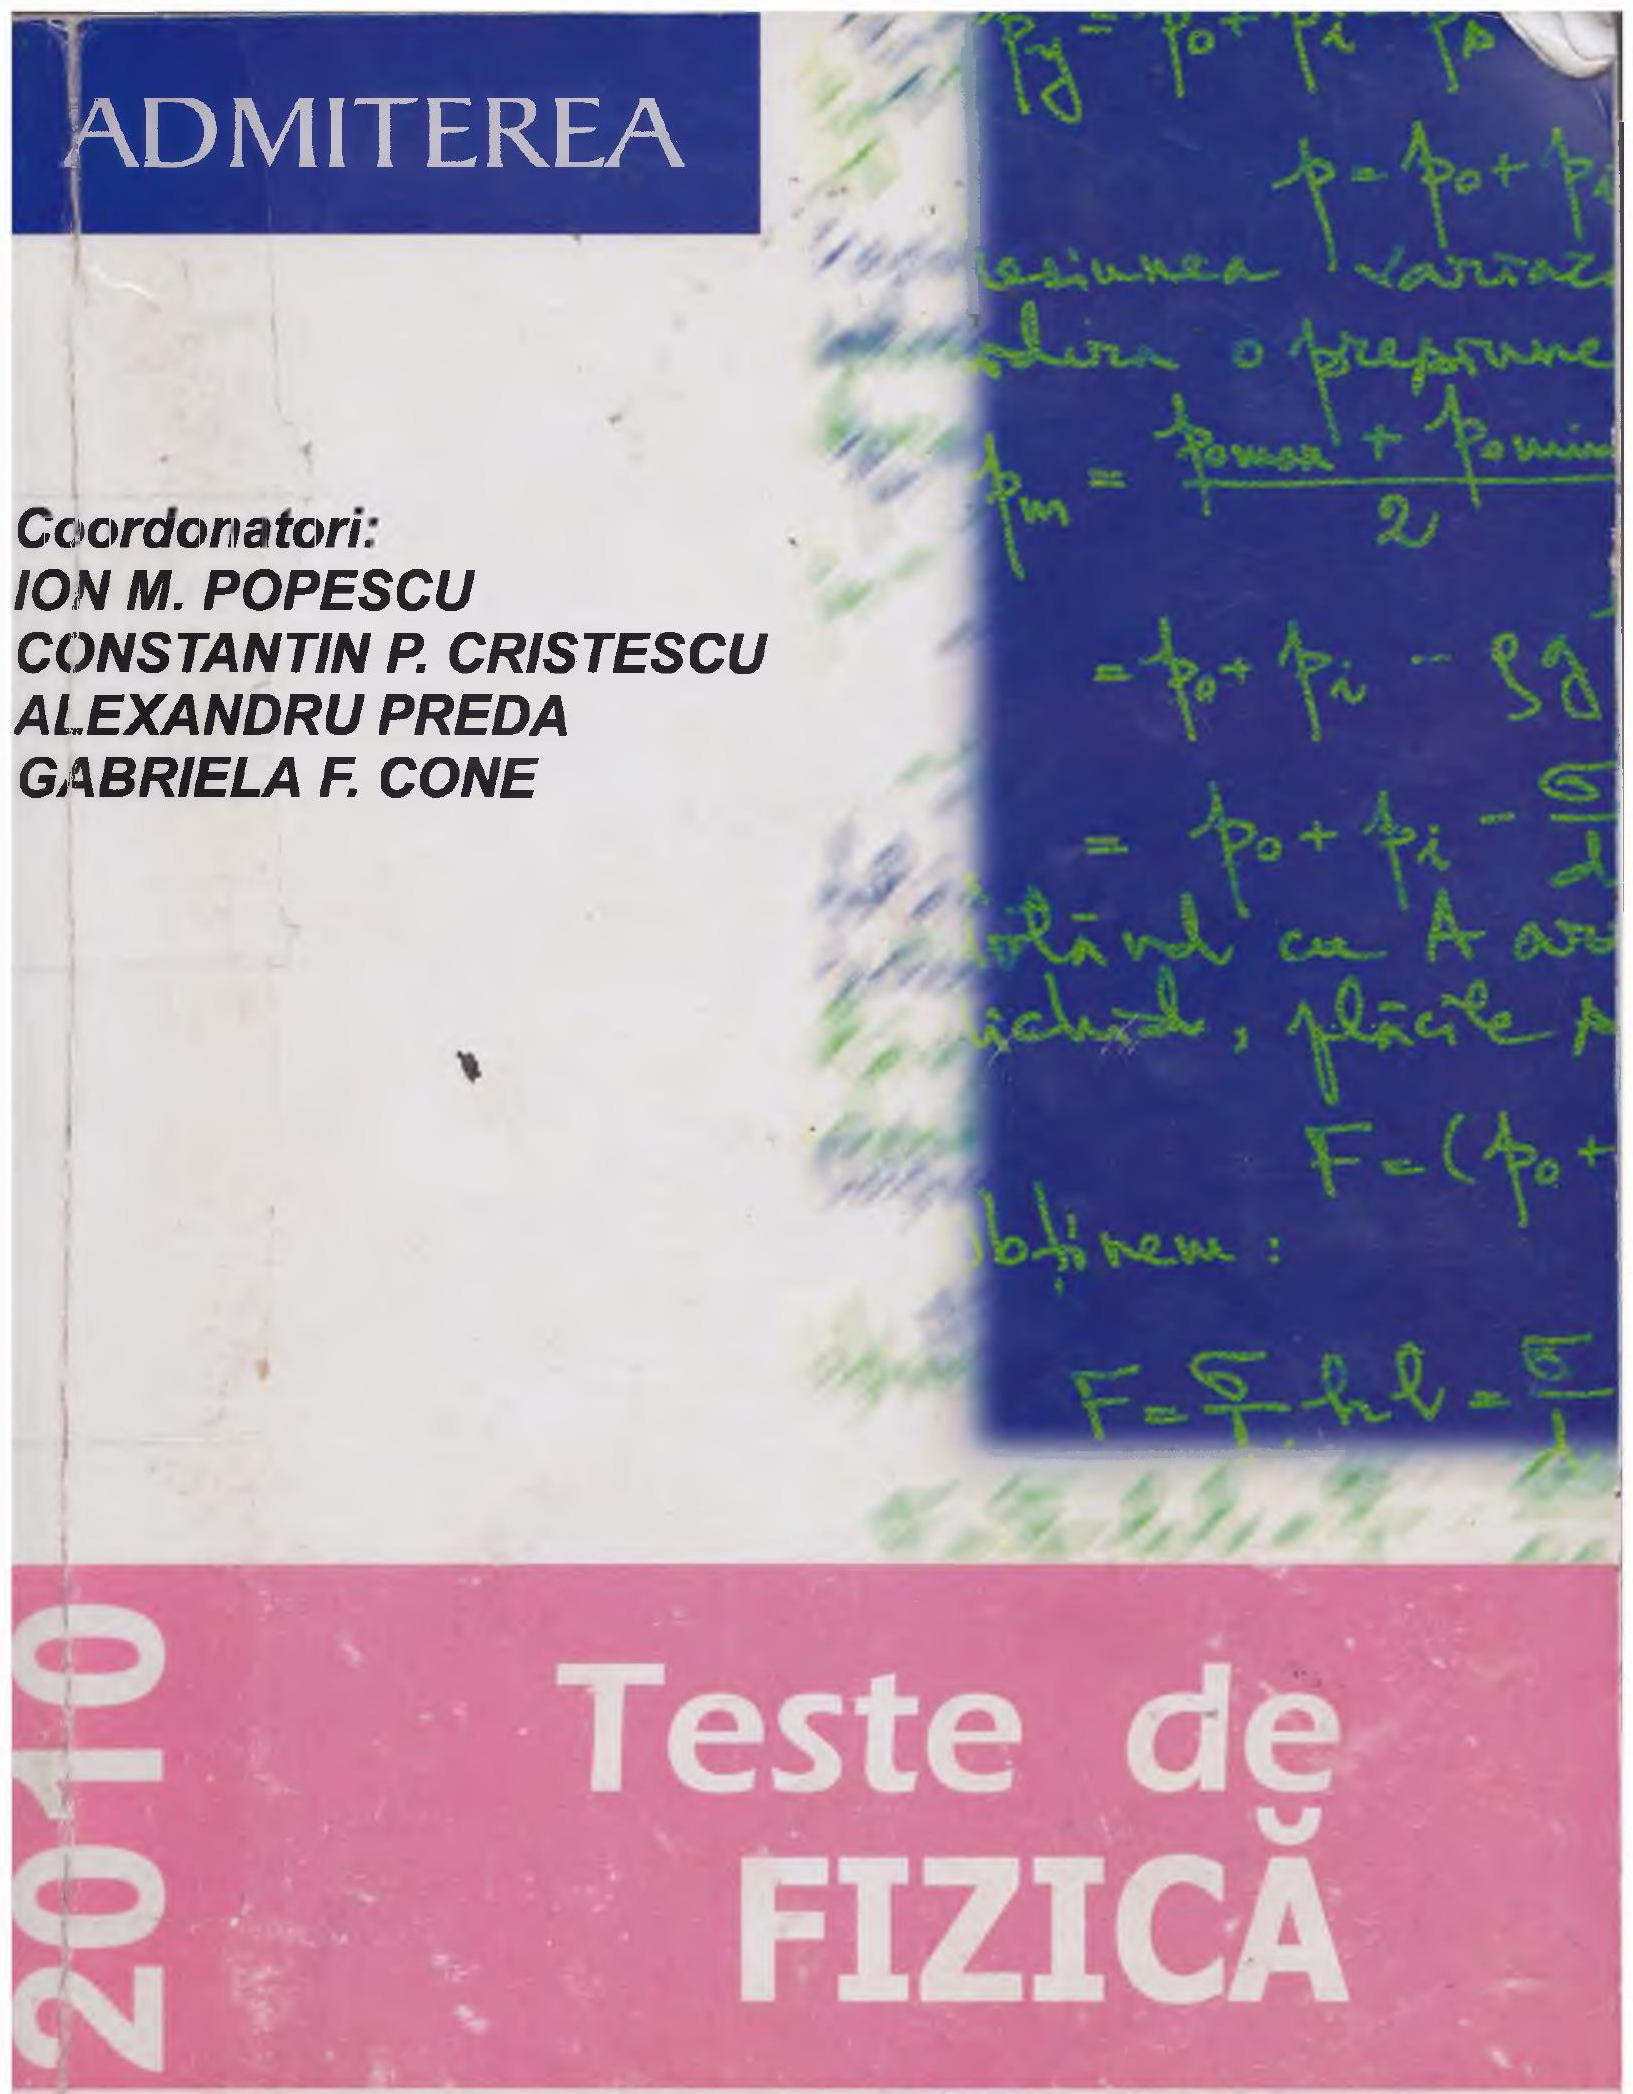
\includegraphics[max width=\textwidth]{2025_07_01_5b3ff9fa0d508c8e9f17g-001}
\end{center}

\section*{CUPRINS}
I. ENUNȚURI ..... 9

\begin{enumerate}
  \item MECANICĂ ..... 11
  \item FIZICĂ MOLECULARĂ ŞI TERMODINAMICĂ ..... 81
  \item ELECTRICITATE ŞI MAGNETISM ..... 152\\
II. RĂSPUNSURI ..... 201
  \item MECANICĂ ..... 203
  \item FIZICĂ MOLECULARĂ ŞI TERMODINAMICĂ ..... 204
  \item ELECTRICITATE ŞI MAGNETISM ..... 205\\
III. REZOLVĂRI ..... 207
  \item MECANICĂ ..... 209
  \item FIZICĂ MOLECULARĂ ŞI TERMODINAMICĂ ..... 281
  \item ELECTRICITATE ŞI MAGNETISM ..... 350
\end{enumerate}

\section*{1. MECANICĂ*}
1.1.* Dacă o particulă de masă $m$ ce se mişcă cu viteza $v$ ciocneşte elastic o particulă de masă $2 m$ ce se află în repaus şi ricoşează de unde a venit, energiile cinetice finale ale celor două particule sunt:\\ A) $\frac{m v^{2}}{2}, m v^{2}$; B) $\frac{3}{2} m v^{2}, \frac{3}{4} m v^{2}$; C) $\frac{m v^{2}}{18}, m v$; D) $m v^{2}, \frac{3}{2} m v^{2}$; E) $m v^{2}, \frac{4}{9} m v^{2}$; F) $\frac{m v^{2}}{18}, \frac{4}{9} m v^{2}$.\\ (Ion M. Popescu)\\

1.2. Acceleraţia de $12960 \mathrm{~km} / \mathrm{h}^{2}$ în $\mathrm{m} / \mathrm{s}^{2}$ este:\\ A) $1 \mathrm{~m} / \mathrm{s}$; B) $1,5 \mathrm{~ms}$; C) $1,2 \mathrm{~m} / \mathrm{s}^{2}$; D) $2 \mathrm{~m} / \mathrm{s}^{2}$; E) $1 \mathrm{~m} / \mathrm{s}^{2}$; F) $1,5 \mathrm{~m} / \mathrm{s}^{2}$.\\ (Ion M. Popescu)\\

1.3.* Un vagonet de masă $m_{1}=200 \mathrm{~kg}$ se mişcă cu viteza $v_{1}=5 \mathrm{~m} / \mathrm{s}$. În vagonet cade vertical un sac cu masa $m_{2}=50 \mathrm{~kg}$, viteza acestuia devenind:\\ A) $3 \mathrm{~m} / \mathrm{s}$; B) $5 \mathrm{~m} / \mathrm{s}$; C) $4 \mathrm{~m} / \mathrm{s}$; D) $2 \mathrm{~m} / \mathrm{s}$; E) $6 \mathrm{~m} / \mathrm{s}$; F) $10 \mathrm{~m} / \mathrm{s}$.\\ (Ion M. Popescu)\\

1.4. Accelerația gravitațională este $g=10 \mathrm{~m} / \mathrm{s}^{2}$. Lucrul mecanic efectuat de o macara care ridică un corp cu masa $m=300 \mathrm{~kg}$ la înălțimea $h=5 \mathrm{~m}$, cu accelerația $a=2 \mathrm{~m} / \mathrm{s}^{2}$, este:\\ A) $180 \mathrm{~kJ}$; B) $1800 \mathrm{~J}$; C) $16000 \mathrm{~J}$; D) $18 \mathrm{~kJ}$; E) $15 \mathrm{~kJ}$; F) $165 \mathrm{~kJ}$.\\ (Ion M. Popescu)\\

1.5.* Un obuz de masă $M=70 \mathrm{~kg}$ zboară cu viteza $v=320 \mathrm{~m} / \mathrm{s}$. La un moment dat, el explodează în două fragmente, dintre care unul are masa $m_{1}=30 \mathrm{~kg}$ și continuă să se mişte cu viteza $v_{1}=520 \mathrm{~m} / \mathrm{s}$. Cantitatea de energie cinetică ce se creează este:\\ A) $1,05 \mathrm{~MJ}$; B) $1 \mathrm{~MJ}$; C) $10,5 \mathrm{~MJ}$; D) $1060 \mathrm(~kJ}$; E) $0,5 \mathrm{~MJ}$; F) $1 \mathrm{~MJ}$.\\ (Ion M. Popescu)

1.6. O bilă cu masa $m=0,15 \mathrm{~kg}$ cade liber pe un plan orizontal având în momentul ciocnirii viteza $v=12 \mathrm{~m} / \mathrm{s}$. Durata ciocnirii a fost $\Delta t=15 \mathrm{~ms}$. Forța medie de lovire, considerând ciocnirea perfect elastică, este:\\ А) $100 \mathrm{~N}$; B) $90 \mathrm{~N}$; C) $125 \mathrm{~N}$; D) $80 \mathrm{~N}$; E) $240 \mathrm{~N}$; F) $116 \mathrm{~N}$.\\ (Ion M. Popescu)\\

1.7. Pe şoseaua Bucureşti - Ploieşti (lungă de $60 \mathrm{~km}$), pleacă din Bucureşti spre Ploieşti un camion cu viteza $v_{1}=60 \mathrm{~km} / \mathrm{h}$ şi din Ploieşti spre Bucureşti în acelaşi moment, un alt camion cu viteza $v_{2}=50 \mathrm{~km} / \mathrm{h}$. În acelaşi moment dintr-unul din camioane îşi ia zborul spre celălalt camion un porumbel călător, care zboară cu viteza constantă $v_{3}=88 \mathrm{~km} / \mathrm{h}$, până la întâlnirea camioanelor. Care este distanța străbătută de porumbel?\\ A) $50 \mathrm{~km}$; B) $46 \mathrm{~km}$; C) $48 \mathrm{~km}$; D) $160 \mathrm{~km}$; E) $38 \mathrm{~km;}$ F) $30 \mathrm{~km}$.\\ (Ion M. Popescu)\\

1.8. Care dintre următoarele variante pentru formula lui Galilei nu este adevărată?\\ A) $v^{2}=v_{0}^{2}+2 a\left(x-x_{0}\right)$; B) $v^{2}=2 a x$; C) $v^{2}=2 a\left(x-x_{0}\right)$; D) $v^{2}=v_{0}^{2}+2 a v$; E) $v^{2}=v_{0}^{2}+2 a x-2 a x_{0}$; F) $v^{2}=2 a x-2 a x_{0}$.\\ (Ion M. Popescu)\\

1.9. Pe o masă orizontală (cu frecare) un corp de masă $m=0,8 \mathrm{~kg}$ este tras uniform cu ajutorul unui dinamometru care indică o forță $F_{1}=3 \mathrm{~N}$. Când dinamometrul indică forța $F_{2}=7 \mathrm{~N}$, corpul se mişcă cu accelerația:\\ A) $5 \mathrm{~m} / \mathrm{s}^{2}$; B) $6 \mathrm{~m} / \mathrm{s}^{2}$; D) $4 \mathrm{~m} / \mathrm{s}^{2}$; E) $10 \mathrm{~m} / \mathrm{s}^{2}$; F) Nu se poate calcula, deoarece nu se cunoaşte coeficientul de frecare $\mu$.\\ (Ion M. Popescu)\\

1.10. Un punct material de masă $m=1 \mathrm{~kg}$ alunecă fără frecare pe o suprafață curbă PQ (Fig 1.1). Accelerația gravitațională fiind $g=10 \mathrm{~m} / \mathrm{s}$ şi $R=5 \mathrm{~m}$, dacă mişcarea se face fără viteză inițială, viteza punctului material în punctul $Q$ este:\\ A) $8 \mathrm{~m} / \mathrm{s}$; B) $10 \mathrm{~m} / \mathrm{s}^{2}$; C) $4 \mathrm{~m} / \mathrm{s}$; D) $8 \mathrm{~m} / \mathrm{s}^{2}$; E) $20 \mathrm{~m} / \mathrm{s}$; F) $10 \mathrm{~m} / \mathrm{s}$.\\ (Ion M. Popescu)\\ 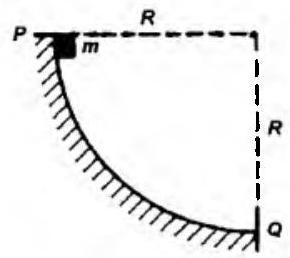
\includegraphics[max width=\textwidth, center]{2025_07_01_5b3ff9fa0d508c8e9f17g-004} Fig 1.1\\

1.11. O săgeată cu masa $m=60 \mathrm{~g}$ este lansată dintr-un arc cu viteza $v_{3}=40 \mathrm{~m} / \mathrm{s}$, pe verticală în sus. Accelerația gravitațională find $g=10 \mathrm{~m} / \mathrm{s}^{2}$, după un timp $t=1 \mathrm{~s}$ de la lansare, energia cinetică a săgeții este:\\ A) $25 \mathrm{~J}$; B) $27 \mathrm{~J}$; C) $30 \mathrm{~J}$; D) $40 \mathrm{~J}$; E) $17 \mathrm{~J}$; F) $1 \mathrm{~J}$.\\ (Ion M. Popescu)

1.12. Un corp se deplasează între punctele $x_{0}=2 \mathrm{~m}$ şi $x=22 \mathrm{~m}$. Când asupra corpului acționează forța care variază liniar cu distanța $F=60-0,5 x, x$ fiind exprimat în metri şi $F$ în Newtoni, lucrul mecanic al forței este:\\ A) $2 \mathrm{~kJ}$; B) $3 \mathrm{~kJ}$; C) $1,08 \mathrm{~kJ}$; D) $3,16 \mathrm{~kJ}$; E) $2,12 \mathrm{~kJ}$; F) $4 \mathrm{~kJ}$.\\ (Ion M. Popescu)\\

1.13. Un vagon de cale ferată cu masa $m=25 \mathrm{~t}$ ciocneşte un obstacol cu viteza $v=0,3 \mathrm{~m} / \mathrm{s}$. Resorturile celor două tampoane comprimându-se cu $x=3 \mathrm{~cm}$, forța maximă care acționează asupra fiecărui resort este (Fiecare tampon are câte un resort.):\\ A) $37 \mathrm{~kN}$; B) $38,5 \mathrm{~kN}$; C) $40 \mathrm{~kN}$; D) $20 \mathrm{~kN}$; E) $37,5 \mathrm{~kN}$; F) $1100 \mathrm{~N}$.\\ (Ion M. Popescu)\\

1.14. Un disc omogen cu raza $R=1 \mathrm{~m}$ şi masa $m=1 \mathrm{~kg}$ se roteşte în jurul axei sale fixe care trece prin centrul său cu viteza liniară $v=1 \mathrm{~m} / \mathrm{s}$. Impulsul său total este:\\ A) $2 \mathrm{~kg} \mathrm{~m} / \mathrm{s}$; B) $1 \mathrm{~kg} \mathrm{~m} / \mathrm{s}$; C) $0 \mathrm{~kg} \mathrm{~m} / \mathrm{s}$; D) $10 \mathrm{~kg} \mathrm{~m} / \mathrm{s}$; E) $40 \mathrm{~kg} \mathrm{~m} / \mathrm{s}$; F) $3 \mathrm{~kg} \mathrm{~m} / \mathrm{s}$.\\ (Ion M. Popescu)\\

% problema: doar 5 variante de raspuns, dintre care 2 identice
1.15.* Două bile de mase $m_{1}=3 \mathrm{~kg}$ şi $m_{2}=2 \mathrm{~kg}$ se mişcă una spre cealaltă cu vitezele $v_{1}=2 \mathrm{~m} / \mathrm{s}$ şi $v_{2}=-3 \mathrm{~m} / \mathrm{s}$. În urma ciocnirii lor plastice se degajă căldura:\\ A) $10 \mathrm{~J}$; B) $9 \mathrm{~J}$; D) $16 \mathrm{~J}$; E) $15 \mathrm{~J}$; F) $16 \mathrm{~J}$.\\ (Ion M. Popescu)\\

1.16. Un automobil accelerează de la starea de repaus la viteza $v=108 \mathrm{~km} / \mathrm{h}$ in $10 \mathrm{~s}$. Forța de tractiune a motorului fiind constantă, distanța parcursă de automobil în acest timp este:\\ A) $150 \mathrm{~m}$; B) $200 \mathrm{~m}$; C) $225 \mathrm{~m}$; D) $120 \mathrm{~m}$; E) $2 \mathrm{~km}$; F) $1 \mathrm{~km}$.\\ (Constantin P. Cristescu)\\

1.17. Un corp cu masa $m=11 \mathrm{~kg}$ este tras de un resort deformat. Constanta elastică a resortului este egală cu $k=50 \mathrm{~N} / \mathrm{m}$, iar coeficientul de frecare dintre corp şi plan este $\mu=\sqrt{3} / 10$. Resortul intins face cu orizontala un unghi $\alpha=60^{\circ}$. Considerând $g=10 \mathrm{~m} / \mathrm{s}^{2}$, energia potențială minimă înmagazinată în resortul deformat necesară pentru a scoate corpul din repaus este:\\ А) $6,5 \mathrm{~J}$; B) $80 \mathrm{~J}$; C) $8,59 \mathrm{~J}$; D) $37,5 \mathrm{~J}$; E) $16 \mathrm{~J}$; F) $1,8 \mathrm{~J}$.\\ (Constantin P. Cristescu)\\

1.18. Un corp este lansat pe verticală în sus de la nivelul solului cu viteza $v_{0}$. Înălțimea față de sol la momentul în care energia cinetică este egală cu un sfert din cea potențială este:\\ А) $\frac{v_{0}^{2}}{4 g}$; B) $\frac{v_{0}^{2}}{2 g}$; C) $\frac{4 v_{0}^{2}}{15 g}$; D) $\frac{2 v_{0}^{2}}{15 g}$; E) $\frac{2 v_{0}^{2}}{5 g}$; F) $\frac{5 v_{0}^{2}}{9 g}$.\\ (Constantin P. Cristescu)\\

1.19. O macara ridică un corp cu greutatea $G=8400 \mathrm{~N}$ la o înălțime $h=35 \mathrm{~m}$ şi apoi îl deplasează orizontal pe o distanţă de $10 \mathrm{~m}$. Neglijând frecările şi considerând $g=10 \mathrm{~m} / \mathrm{s}^{2}$ lucrul efectuat de macara în această operație este:\\ A) $378 \mathrm{~kJ}$; B) $256 \mathrm{~kJ}$; C) $210 \mathrm{~kJ}$; D) $37,8 \mathrm{~kJ}$; E) $29,4 \mathrm{~kJ}$; F) $294 \mathrm{~kJ}$.\\ (Constantin P. Cristescu)\\

1.20. Un corp cu masa $m_{1}=4 \mathrm{~kg}$ agățat de un fir inextensibil este ridicat cu o accelerație $a$. Când un alt corp de masă $m_{2}=6 \mathrm{~kg}$, legat de același fir coboară cu aceeaşi accelerație $a$ (în valoare absolută) tensiunea din fir este aceeași ca în primul caz. Considerând $g=10 \mathrm{~m} / \mathrm{s}^{2}$ accelerația $a$ este:\\ A) $5 \mathrm{~m} / \mathrm{s}^{2}$; B) $2 \mathrm{~m} / \mathrm{s}^{2}$; C) $1 \mathrm{~m} / \mathrm{s}^{2}$; D) $2,5 \mathrm{~m} / \mathrm{s}^{2}$; E) $8 \mathrm{~m} / \mathrm{s}^{2}$; F) $10 \mathrm{~m} / \mathrm{s}^{2}$.\\ (Constantin P. Cristescu)\\

1.21. O forță de $5 \mathrm{~N}$ imprimă unei mase $m_{1}$ o accelerație de $a_{1}=24 \mathrm{~m} / \mathrm{s}^{2}$ și unei alte mase $m_{2}$ o accelerație de $a_{2}=8 \mathrm{~m} / \mathrm{s}^{2}$. Dacă aceeaşi forță acționează asupra ansamblului celor două corpuri, accelerația imprimată este:\\ A) $6 \mathrm{~m} / \mathrm{s}^{2}$; B) $4 \mathrm{~m} / \mathrm{s}^{2}$; C) $11 \mathrm{~m} / \mathrm{s}^{2}$; D) $14 \mathrm{~m} / \mathrm{s}^{2}$; E) $5 \mathrm{~m} / \mathrm{s}^{2}$; F) $20 \mathrm{~m} / \mathrm{s}^{2}$.\\ (Constantin P. Cristescu)\\

1.22. Asupra unui corp cu greutatea $G=20 \mathrm{~N}$ acționează simultan două forțe orizontale $F_{1}=3 \mathrm{~N}$ şi $F_{2}=4 \mathrm{~N}$ orientate pe direcții care fac un unghi de $90^{\circ}$ între ele. Considerând $g=10 \mathrm{~m} / \mathrm{s}^{2}$, accelerația cu care se mişcă corpul pe o suprafață orizontală pentru care coeficientul de frecare este de $0,25$ este:\\ A) $1 \mathrm{~m} / \mathrm{s}^{2}$; B) $0,5 \mathrm{~m} / \mathrm{s}^{2}$; C) $0 \mathrm{~m} / \mathrm{s}^{2}$; D) $0,4 \mathrm{~m} / \mathrm{s}^{2}$; E) $0,2 \mathrm{~m} / \mathrm{s}^{2}$; F) $0,35 \mathrm{~m} / \mathrm{s}^{2}$.\\ (Constantin P. Cristescu)\\

1.23. Un tren trece cu viteza $v=26 \mathrm{~m} / \mathrm{s}$ paralel cu un zid lung. Un călător din tren produce un sunet puternic şi aude ecoul (reflectat de perete) după un timp de $2 \mathrm{~s}$. Dacă sunetul se propagă cu viteza $v_{s}=340 \mathrm{~m} / \mathrm{s}$, distanţa dintre calea ferată şi zid este:\\ A) $310 \mathrm{~m}$; B) $314 \mathrm{~m}$; C) $308 \mathrm{~m}$; D) $339 \mathrm{~m}$; E) $336 \mathrm{~m}$; F) $324 \mathrm{~m}$.\\ (Constantin P. Cristescu)\\

1.24. Un automobil urcă o pantă cu $\alpha=\left(\frac{9}{\pi}\right)$ grade fără motor, viteza sa inițială la baza pantei fiind de $v_{0}=72 \mathrm{~km} / \mathrm{h}$. Considerând $g=10 \mathrm{~m} / \mathrm{s}^{2}$, facând aproximația $\sin \alpha=\alpha rad$ şi neglijând frecările, timpul în care viteza automobilului se reduce la $v=18 \mathrm{~km} / \mathrm{h}$ este:\\ A) $20 \mathrm{~s}$; B) $30 \mathrm{~s}$; C) $40 \mathrm{~s}$; D) $25 \mathrm{~s}$; E) $34 \mathrm{~s}$; F) $18 \mathrm{~s}$.\\ (Constantin P. Cristescu)\\

1.25. Un corp de dimensiuni mici este aruncat de la nivelul solului pe verticală în sus. Dacă el se află în aer timp de $4 \mathrm{~s}$, aproximând $g=10 \mathrm{~m} / \mathrm{s}^{2}$, înălțimea maximă atinsă de corp este:\\ A) $20 \mathrm{~m}$; B) $18 \mathrm{~m}$; C) $24 \mathrm{~m}$; D) $15 \mathrm{~m}$; E) $45 \mathrm{~m}$; F) $30 \mathrm{~m}$.\\ (Constantin P. Cristescu)\\

1.26. Un corp lansat pe o suprafaţă orizontală cu viteza inițială $v_{0}=20 \mathrm{~m} / \mathrm{s}$ parcurge în secunda a cincea distanţa de $5 \mathrm{~m}$. Considerând $g=10 \mathrm{~m} / \mathrm{s}^{2}$, coeficientul de frecare este:\\ А) $0,4$; B) $0,08$; C) $1 / 3$; D) $\sqrt{3} / 6$; E) $0,2 / 3$; F) $1 / 6$.\\ (Constantin P. Cristescu)\\

1.27.* Un vagon de tren cu masa $m_{1}=21 \mathrm{~t}$ şi cu viteza de $v_{1}=6 \mathrm{~m} / \mathrm{s}$ ciocneşte un alt vagon cu masa $m_{2}=49 \mathrm{t}$ care se mişcă în acelaşi sens cu viteza de $v_{2}=3 \mathrm{~m} / \mathrm{s}$, astfel încât după ciocnire ele se mişcă împreună. Viteza ansamblului celor două vagoane este:\\ A) $5 \mathrm{~m} / \mathrm{s}$; B) $4,8 \mathrm{~m} / \mathrm{s}$; C) $3,2 \mathrm{~m} / \mathrm{s}$; D) $4,1 \mathrm{~m} / \mathrm{s}$; E) $3,9 \mathrm{~m} / \mathrm{s}$; F) $4,5 \mathrm{~m} / \mathrm{s}$.\\ (Constantin P. Cristescu)\\

1.28. Un avion care zboară cu viteza constantă $v=360 \mathrm{~km} / \mathrm{h}$, descrie o buclă circulară în plan vertical. Considerând $g=10 \mathrm{~m} / \mathrm{s}^{2}$, raza maximă posibilă a buclei este:\\ A) $1 \mathrm{~km}$; B) $2 \mathrm{~km}$; C) $800 \mathrm{~m}$; D) $1,6 \mathrm{~km}$; E) $500 \mathrm{~m}$; F) $1250 \mathrm{~m}$.\\ (Constantin P. Cristescu)\\

1.29. Un automobil se deplasează pe un pod convex de forma unui arc de cerc cu raza $r=22,5 \mathrm{~m}$. Considerând $g=10 \mathrm{~m} / \mathrm{s}^{2}$, viteza maximă pentru care automobilul rămâne în contact cu podul în punctul cel mai de sus este:\\ A) $120 \mathrm{~km} / \mathrm{h}$; B) $72 \mathrm{~km} / \mathrm{h}$; C) $20 \mathrm{~m} / \mathrm{s}$; D) $17 \mathrm{~m} / \mathrm{s}$; E) $15 \mathrm{~m} / \mathrm{s}$; F) $30 \mathrm{~m} / \mathrm{s}$.\\ (Constantin P. Cristescu)\\

1.30.* Două sfere de mase $m_{1}$ şi $m_{2}$ având viteze egale şi orientate în sens opus se ciocnesc perfect elastic. După ciocnire, sfera de masă $m_{1}$ rămâne în repaus. Raportul maselor celor două sfere $m_{1} / m_{2}$ este:\\ A) $1 / 2$; B) $3$; C) $2$; D) $4,5$; E) $0,8$; F) $5$.\\ (Constantin P. Cristescu)\\

1.31. Un corp cu masa $m=1 \mathrm{~kg}$ legat cu o sârmă cu lungimea $l_{0}=1 \mathrm{~m}$ este rotit astfel încât descrie o traiectorie aproximativ circulară în plan vertical. Viteza constantă a corpului este astfel încât forța centrifugă este dublul greutății corpului. Modulul de elasticitate al sârmei este $E=10^{11} \mathrm{~N} / \mathrm{m}^{2}$, iar secțiunea sa este $S=0,5 \cdot 10^{-6} \mathrm{~m}^{2}$. În cursul mişcării lungimea sârmei variază în intervalul:\\ A) $(100,02 \div 100,06) \mathrm{cm}$; B) $(100,10 \div 100,30) \mathrm{cm}$; C) $(100,01 \div 100,05) \mathrm{cm}$; D) $(100,05 \div 100,10) \mathrm{cm}$; E) $(100,04 \div 100,09) \mathrm{cm}$; F) $(100,03 \div 100,06) \mathrm{cm}$.\\ (Constantin P. Cristescu)\\

1.32. Două corpuri cu masele $m_{1}$ şi $m_{2}$ sunt legate unul de altul cu un fir de masă neglijabilă. Asupra corpului de masă $m_{1}$ acționează o forță orizontală $F$, iar coeficientul de frecare dintre corpuri şi suprafața orizontală pe care se află este $\mu$. Tensiunea din firul de legătură este:\\ A) $\frac{F m_{1}}{m_{1}+m_{2}}$; B) $\frac{F m_{2}}{m_{1}+m_{2}}$; C) $\frac{F m_{1} m_{2}}{\left(m_{1}+m_{2}\right)^{2}}$; D) $F-\mu m_{2} g$; E) $\frac{F\left(m_{1}+m_{2}\right)}{m_{2}}$; F) $F-\mu\left(m_{1}+m_{2}\right) g$.\\ (Constantin P. Cristescu)\\

1.33. Un corp este lansat de jos in sus pe un plan înclinat de unghi $\alpha=30^{\circ}$. Dacã timpul de coborâre este de $n=4$ ori mai mare decât cel de urcare, coeficientul de frecare dintre corp şi plan este:\\ A) $\frac{\sqrt{3}}{10}$; B) $\frac{2 \sqrt{3}}{15}$; C) $\frac{\sqrt{3}}{8}$; D) $\frac{\sqrt{3}}{12}$ E) $\frac{5 \sqrt{3}}{17}$; F) $\frac{3 \sqrt{3}}{10}$.\\ (Constantin P. Cristescu)\\

1.34. Mişcarea unui corp este descrisă de ecuația $x=8+20 t-2 t^{2}$ unde $x$ este în metri şi $t$ este în secunde. Viteza corpului la momentul $t=2,3 \mathrm{~s}$ este:\\ А) $10,7 \mathrm{~m} / \mathrm{s}$; B) $15 \mathrm{~m} / \mathrm{s}$; C) $8,8 \mathrm{~m} / \mathrm{s}$; D) $18 \mathrm{~m} / \mathrm{s}$; E) $11,2 \mathrm{~mm} / \mathrm{s}$; F) $10,8 \mathrm{~m} / \mathrm{s}$.\\ (Constantin P. Cristescu)\\

1.35. Ecuația vitezei unui corp este $v=12-t$ unde $v$ este măsurat în $\mathrm{m} / \mathrm{s}$, iar $t$ în secunde. Dacă inițial $(t=0)$ coordonata de poziție a corpului este $x_{0}=10 \mathrm{~m}$, coodonata la momentul $t=8 \mathrm{~s}$ este:\\ A) $74 \mathrm{~m}$; B) $16 \mathrm{~m}$; C) $32 \mathrm{~m}$; D) $124 \mathrm{~m}$; E) $65 \mathrm{~m}$; F) $108 \mathrm{~m}$.\\ (Constantin P. Cristescu)\\

1.36. Un corp cu masa $m=4,2 \mathrm{~kg}$ este lansat în jos pe un plan înclinat cu unghiul $\alpha$ dat de $\operatorname{tg} \alpha=\mu, \mu$ find coeficientul de frecare. Dacă înălțimea inițială a corpului față de baza planului este $h=2,5 \mathrm{~m}$ şi se consideră $g=10 \mathrm{~m} / \mathrm{s}^{2}$, lucrul mecanic consumat prin frecare de-a lungul planului este:\\ A) $230 \mathrm{~J}$; B) $175 \mathrm{~J}$; C) $105 \mathrm{~J}$; D) $208 \mathrm{~J}$; E) $244 \mathrm{~J}$; F) $98 \mathrm{~J}$.\\ (Constantin P. Cristescu)\\

% atentie: variantele de raspuns sunt in totalitate imagini
1.37. Un corp aflat la o înălțime oarecare este aruncat în direcție orizontală cu viteza $v_{0}$. Graficul vitezei corpului ca funcție de timp are forma:\\ (Alexandru M. Preda)\\ 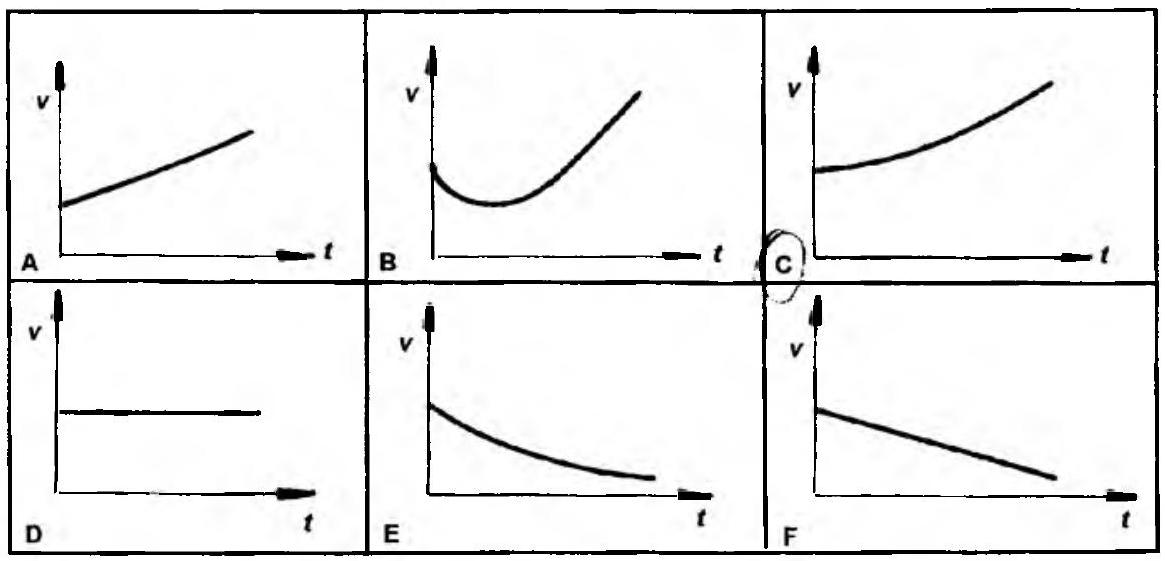
\includegraphics[max width=\textwidth, center]{2025_07_01_5b3ff9fa0d508c8e9f17g-010(2)}\\

1.38. Cu o armă având lungimea țevii $l=25 \mathrm{~cm}$ şi secțiunea interioară $A=80 \mathrm{~mm}^{2}$ se trage un glonț cu masa $m=50 \mathrm{~g}$. Dacă glonțul parcurge lungimea țevii sub acțiunea unei presiuni constante $p=2 \cdot 10^{8} \mathrm{~N} / \mathrm{m}^{2}$ şi considerând frecarea neglijabilă, viteza glonțului la ieşirea din țeavă este:\\ A) $55 \mathrm{~m} / \mathrm{s}$; B) $400 \mathrm{~m} / \mathrm{s}$; C) $500 \mathrm{~m} / \mathrm{s}$; D) $375 \mathrm{~m} / \mathrm{s}$; E) $440 \mathrm{~m} / \mathrm{s}$; F) $620 \mathrm{~m} / \mathrm{s}$.\\ (Alexandru M. Preda)\\

1.39. Asupra unui corp cu masa $m=3 \mathrm{~kg}$ aflat pe o suprafață pe care se poate mişca fară frecare, acționează o forţă care depinde de timp conform graficului din Fig.1.2. Cunoscând că $v_{0}=0$, la sfârşitul celei de a 5-a secunde viteza corpului este:\\ A) $11 \mathrm{~m} / \mathrm{s}$; B) $10 \mathrm{~m} / \mathrm{s}$; C) $12,5 \mathrm{~m} / \mathrm{s}$; D) $12 \mathrm{~m} / \mathrm{s}$; E) $14 \mathrm{~m} / \mathrm{s}$; F) $9,5 \mathrm{~m} / \mathrm{s}$.\\ (Alexandru M. Preda)\\ 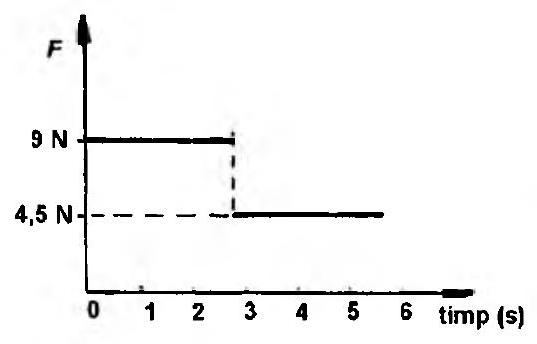
\includegraphics[max width=\textwidth, center]{2025_07_01_5b3ff9fa0d508c8e9f17g-010(1)} Fig. 1.2\\ 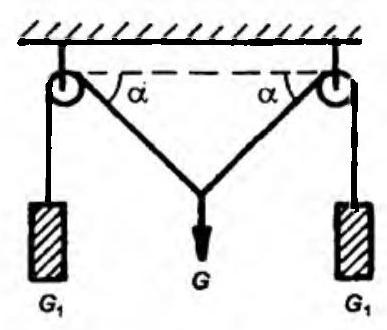
\includegraphics[max width=\textwidth, center]{2025_07_01_5b3ff9fa0d508c8e9f17g-010} Fig. 1.3\\

% atentie: variantele de raspuns sunt in totalitate imagini
1.40. Un corp de greutate $G$ este suspendat ca în Fig. 1.3. Care dintre graficele de mai jos reprezintă dependenta de unghiul $\alpha$ a greutății $G_{1}$ care asigură echilibrul sistemului?\\ (Alexandru M. Preda)\\ 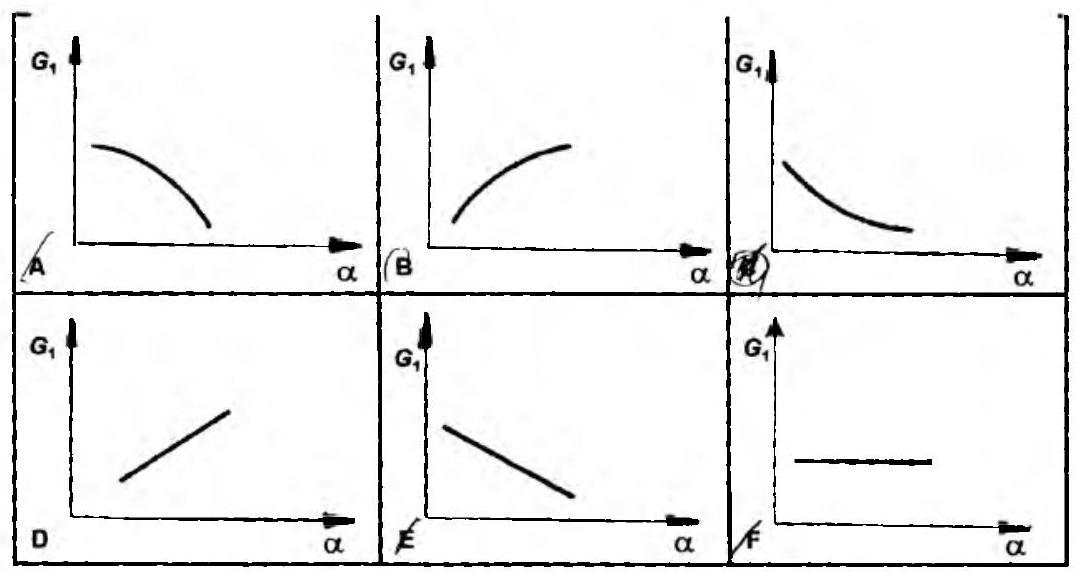
\includegraphics[max width=\textwidth, center]{2025_07_01_5b3ff9fa0d508c8e9f17g-011(2)}\\

1.41. Un automobil cu masa $m=800 \mathrm{~kg}$ se deplasează cu viteza $v_{0}=10 \mathrm{~m} / \mathrm{s}$. Şoferul observă un obstacol aflat în față la distanță $d=6,4 \mathrm{~m}$ de autombil și acționează frâna. Ştiind că forța de frânare asigură oprirea completă pe o distanță de $10 \mathrm{~m}$, impulsul pe care îl transferă automobilul obstacolului la ciocnire este:\\ A) $2300 \mathrm{~kg} \mathrm{~m} / \mathrm{s}$; B) $4800 \mathrm{~kg} \mathrm{~m} / \mathrm{s}$; C) $5200 \mathrm{~kg} \mathrm{~m} / \mathrm{s}$; D) $6350 \mathrm{~kg} \mathrm{~m} / \mathrm{s}$; E) $3850 \mathrm{~kg} \mathrm{~m} / \mathrm{s}$; F) $5000 \mathrm{~kg} \mathrm{~m} / \mathrm{s}$.\\ (Alexandru M. Preda)\\

% atentie: variantele de raspuns sunt in totalitate imagini
1.42. Care dintre graficele de mai jos corespunde dependenţei de timp a vitezei unei bile aruncate vertical în sus şi care în cădere suferă ciocniri perfect elastice și instantanee cu o suprafață plană orizontală? Momentul inițial este momentul aruncării.\\ (Alexandru M. Preda)\\ 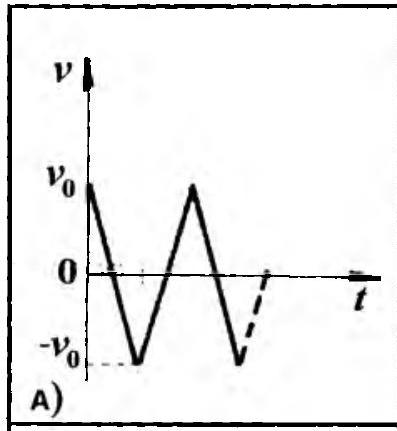
\includegraphics[max width=\textwidth, center]{2025_07_01_5b3ff9fa0d508c8e9f17g-011}\\ \includegraphics[max width=\textwidth, center]{2025_07_01_5b3ff9fa0d508c8e9f17g-011(1)}\\ \includegraphics[max width=\textwidth, center]{2025_07_01_5b3ff9fa0d508c8e9f17g-012(1)}\\

1.43. Un corp cade liber de la o înățime $h$. După un interval de timp $\tau$ de la pornirea primului corp, cade liber de la aceeaşi înălțime, un al doilea corp. Ce fel de mişcare execută primul corp față de al doilea corp?\\ A) Uniform accelerată cu $a=g$; B) Uniform acceleratã cu $a=g / 2$; C) Uniform accelerată cu $a=2 g$; D) Uniformă; E) Accelerată cu accelerație variabilă; F) Uniform încetinită cu acceleraţia $a=g / 2$.\\ (Maria Honciuc)\\

1.44. Un mobil se mişcă uniform cu viteza $v_{1}=5 \mathrm{~m} / \mathrm{s}$. La un moment dat, un alt mobil care vine din acelaşi sens, aflat la distanța $d$ de primul, începe să frâneze de la viteza $v_{2}=10 \mathrm{~m} / \mathrm{s}$. Acceleraţia de frânare este $a=0,1 \mathrm{~m} / \mathrm{s}^{2}$. Care este spațiul parcurs de primul mobil, până la prima intâlnire a mobilelor? (Mobilele se întâlnesc o singură dată).\\ A) $250 \mathrm{~m}$; B) $125 \mathrm{~m}$; C) $500 \mathrm{~m}$; D) $175 \mathrm{~m}$; E) $300 \mathrm{~m}$; F) $50 \mathrm{~m}$.\\ (Maria Honciuc)\\

1.45. Fie sistemul format din masele $m_{1}$ şi $m_{2}=3 m_{1}$ care sunt legate printr-un fir inextensibil, de greutate neglijabilă, trecut peste un scripete, ca în Fig. 1.4. Se cunoaşte coeficientul de frecare pe planul orizontal $\mu=0,15$. Sistemul se mişcă cu accelerația $a_{1}$. Dacă schimbăm locul corpurilor între ele, sistemul se mişcă cu accelerația $a_{2}$. Găsiți care este relația dintre accelerații:\\ A) $a_{1}=2,5 a_{2}$; B) $a_{1}=3 a_{2}$; C) $a_{1}=3,5 a_{2}$; D) $a_{1}=5,18 a_{2}$; E) $a_{1}=3,15 a_{2}$; F) $a_{1}=5,7 a_{2}$.\\ (Maria Honciuc)\\ 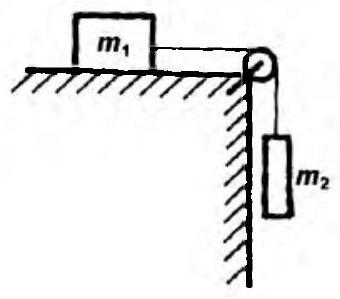
\includegraphics[max width=\textwidth, center]{2025_07_01_5b3ff9fa0d508c8e9f17g-012} Fig. 1.4\\

1.46. Doi pietoni aflați în localitățile A şi B pornesc unul spre altul în acelaşi moment, într-o mişcare rectilinie uniformă. În momentul întâlnirii, primul parcursese cu $1,5 \mathrm{~km}$ mai mult decât celălalt. După întâlnire, pietonii își continuă drumul. Primul ajunge în localitatea B după un timp $t_{1}$ de la intâlnire, iar al doilea ajunge în localitatea A dupã un timp $t_{2}$. Dacă $t_{1}=30$ minute şi $t_{2}=1$ oră, vitezele cu care se mişcă cei doi pietoni sunt:\\ A) $v_{1}=2 \mathrm{~m} / \mathrm{s}, v_{2}=1,42 \mathrm{~m} / \mathrm{s}$; B) $v_{1}=7,2 \mathrm{~km} / \mathrm{h}, v_{2}=10 \mathrm{~km} / \mathrm{h}$; C) $v_{1}=7,2 \mathrm{~km} / \mathrm{h}, v_{2}=5,5 \mathrm{~km} / \mathrm{h}$; D) $v_{2}=3 \mathrm{~m} / \mathrm{s}, v_{2}=5 \mathrm{~km} / \mathrm{h}$; E) $v_{1}=7,2 \mathrm{~km} / \mathrm{h}, v_{2}=1,5 \mathrm{~m} / \mathrm{s}$; F) $v_{1}=5 \mathrm{~m} / \mathrm{s}, v_{2}=7,2 \mathrm{~m} / \mathrm{s}$.\\ (Maria Honciuc)\\

1.47. Un corp este menținut în echilibru pe un plan înclinat de unghi $\alpha$ față de orizontală, fie cu o forță minimă orizontală, fie cu o forță minimă normală pe plan de $k$ ori mai mare decât prima. Coeficientul de frecare dintre corp și plan este:\\ A) $\mu=\frac{\sin \alpha}{k-\sin \alpha}$; B) $\mu=\frac{\cos \alpha}{k+\sin \alpha}$; C) $\mu=\frac{\cos \alpha}{k-\sin \alpha}$; D) $\mu=\frac{k}{k-\sin \alpha}$; E) $\mu=\frac{\cos ^{2} \alpha}{k-\sin \alpha}$; F) $\mu=\frac{\cos \alpha}{k \cos \alpha-\sin \alpha}$.\\ (Maria Honciuc)\\

1.48. Un corp este lansat în sus, pe un plan înclinat de unghi $\alpha=30^{\circ}$ cu orizonatala şi apoi revine la baza planului. Dacă timpul de urcare este de $k=1,1$ ori mai mic decât timpul de coborâre, coeficientul de frecare dintre corp şi planul înclinat este:\\ A) $\mu=0,5$; B) $\mu=0,8$; C) $\mu=0,25$; D) $\mu=0,45$; E) $\mu=0,055$; F) $\mu=0,455$.\\ (Maria Honciuc)\\

1.49. Un mobil este aruncat cu viteza inițială $v_{0}$, pe verticală, în sus. Momentele de timp la care energia cinetică a corpului este egală cu energia potențială sunt:\\ A) $t_{1,2}=\frac{2 v_{0} \pm \sqrt{2}}{2 g}$; B) $t_{1,2}=\frac{v_{0}(2 \pm \sqrt{2})}{g}$; C) $t_{1,2}=\frac{v_{0}(2 \pm \sqrt{2})}{2}$; D) $t_{1,2}=\frac{v_{0}(2 \mp \sqrt{3})}{2 g}$; E) $t_{1,2}=\frac{v_{0}(1 \pm \sqrt{2})}{2 g}$; F) $t_{1,2}=\frac{v_{0}(2 \pm \sqrt{2})}{2 g}$.\\ (Maria Honciuc)\\

1.50.* Acele unui ceasornic indică ora 12. Să se determine timpul după care orarul şi minutarul sunt prima dată perpendiculare, respectiv din nou suprapuse.\\ A) $t_{1}=1,63 \mathrm{~min}, t_{2}=1,09 \mathrm{~min}$; B) $t_{1}=900 \mathrm{~s}, t_{2}=1,09 \mathrm{~h}$; C) $t_{1}=16,36 \mathrm{~min}, t_{2}=65,45 \mathrm{~min}$; D) $t_{1}=981,6 \mathrm{~s}, t_{2}=300 \mathrm{~min}$; E) $t_{1}=900 \mathrm{~s}, t_{2}=65 \mathrm{~min}$; F) $t_{1}=16,36 \mathrm{~min}, t_{2}=6,55 \mathrm{~min}$.\\ (Maria Honciuc)\\

1.51. Un corp cade liber de la înălțimea $h$, iar altul este lansat simultan pe vertícală de la suprafața Pământului. Ce înălțime maximă va atinge al doilea mobil, știind că ambele corpuri ating simultan solul.\\ A) $h$; B) $h / 2$; C) $h / 4$; D) $2 h$; E) $\sqrt{h}$; F) $h / 3$.\\ (Corneliu Ghizdeanu)\\

1.52. O minge este lansată pe verticală de la sol cu viteza inițială $v_{0}=40 \mathrm{~m} / \mathrm{s}$. Se cere înălțimea maximă la care ajunge mingea după ciocnirea cu solul, dacă sărind pierde instantaneu jumătate din energia pe care o posedă în momentul atingerii solului ($g=10 \mathrm{~m} / \mathrm{s}^{2}$).\\ A) $80 \mathrm{~m}$; B) $60 \mathrm{~m}$; C) $40 \mathrm{~m}$; D) $20 \mathrm{~m}$; E) $40 \sqrt{2} \mathrm{~m}$; F) $55 \mathrm{~m}$.\\ (Corneliu Ghizdeanu)\\

1.53. Din acelaşi punct, aflat la înălțimea $h_{0}=245 \mathrm{~m}$ deasupra solului, sunt lăsate să cadă liber, la un interval de timp $\Delta t=2 \mathrm{~s}$, două corpuri. Se cere distanța maximă dintre corpurile aflate încă în aer ($g=10 \mathrm{~m} / \mathrm{s}^{2}$).\\ A) $200 \mathrm{~m}$; B) $120 \mathrm{~m}$; C) $24,5 \mathrm{~m}$; D) $140 \mathrm{~m}$; E) $150 \mathrm{~m}$; F) $145 \mathrm{~m}$.\\ (Corneliu Ghizdeanu)\\

1.54. O bilă este atârnată de un fir subțire de lungime $l=0,2 \mathrm{~m}$ şi scoasă succesiv din poziția de echilibru cu unghiurile $\alpha_{1}=45^{\circ}$, respectiv $\alpha_{2}=30^{\circ}$ şi apoi este lăsată liberă. Se cere raportul vitezelor cu care bila trece prin poziția de echilibru pentru cele două situații ($g=10 \mathrm{~m} / \mathrm{s}^{2}$).\\ A) $1$; B) $2$; C) $2,45$; D) $1,478$; E) $0,5$; F) $1,25$.\\ (Corneliu Ghizdeanu)\\

1.55. Un glonte pătrunde într-o scândură pe o distanță $d$ având o viteză inițială $v_{0}=200 \mathrm{~m} / \mathrm{s}$. Să se calculeze viteza $v$ cu care iese glontele dintr-o scândură din acelaşi material, care are grosimea pe jumătate.\\ A) $200 \mathrm{~m} / \mathrm{s}$; B) $150 \mathrm{~m} / \mathrm{s}$; C) $125,5 \mathrm{~m} / \mathrm{s}$; D) $141 \mathrm{~m} / \mathrm{s}$; E) $98 \mathrm{~m} / \mathrm{s}$; F) $140 \mathrm{~m} / \mathrm{s}$.\\ (Corneliu Ghizdeanu)\\

1.56. Un tren cu masa totală $m=200 \mathrm{t}$ este tras pe o linie orizontală de o locomotivă cu puterea $P=400 \mathrm{~kW}$. Coeficientul de frecare dintre tren şi şine este $\mu=0,01$. Se cere accelerația sa în momentul când viteza are valoarea $v=2 \mathrm{~m} / \mathrm{s}$ cât şi valoarea vitezei maxime ($g=10 \mathrm{~m} / \mathrm{s}^{2}$).\\ A) $1,9 \mathrm{~m} / \mathrm{s}^{2}, 10 \mathrm{~m} / \mathrm{s}$; B) $2 \mathrm{~m} / \mathrm{s}^{2}, 10 \mathrm{~m} / \mathrm{s}$; C) $0,9 \mathrm{~m} / \mathrm{s}^{2}, 20 \mathrm{~m} / \mathrm{s}$; D) $1,9 \mathrm{~m} / \mathrm{s}^{2}, 20 \mathrm{~m} / \mathrm{s}$; E) $0,9 \mathrm{~m} / \mathrm{s}^{2}, 40 \mathrm{~m} / \mathrm{s}$; F) $0,5 \mathrm{~m} / \mathrm{s}^{2}, 20 \mathrm{~m} / \mathrm{s}$.\\ (Corneliu Ghizdeanu)\\

1.57.* Pentru un pendul conic se cunosc: $l, \alpha, g$. Perioada lui de rotație este:\\ A) $2\pi \lfloor \sqrt{l \cos \alpha / g} \rfloor$; B) $2\pi \lfloor \sqrt{l / g} \rfloor$; C) $2\pi \lfloor \sqrt{l \sin \alpha / g} \rfloor$; D) $2\pi \lfloor \sqrt{l \tan \alpha / g} \rfloor$; E) $2\pi \lfloor \sqrt{m / (l \cos \alpha \cdot g)} \rfloor$; F) $2\pi \lfloor \sqrt{m / (l \sin \alpha \cdot g)} \rfloor$.\\ (Corneliu Ghizdeanu)\\

1.58. Un corp cu $m=1 \mathrm{~kg}$ se mişcă uniform accelerat fară viteză inițială parcurgând în prima secundă $0,5 \mathrm{~m}$. Cât este energia cinetică a corpului după $2 \mathrm{~s}$?\\ А) $2 \mathrm{~J}$; B) $10 \mathrm{~J}$; C) $0,1 \mathrm{~J}$; D) $20 \mathrm{~J}$; E) $0,2 \mathrm{~J}$; F) $0,01 \mathrm{~J}$.\\ (Niculae N. Puşcaş)\\

1.59. Un corp se mişcă uniform accelerat parcurgând în prima secundă $1 \mathrm{~m}$, iar în a doua secundă $2 \mathrm{~m}$. Cât este accelerația corpului?\\ A) $10 \mathrm{~m} / \mathrm{s}^{2}$; B) $5 \mathrm{~m} / \mathrm{s}^{2}$; C) $0,1 \mathrm{~m} / \mathrm{s}^{2}$; D) $4 \mathrm{~m} / \mathrm{s}^{2}$; E) $0,01 \mathrm{~m} / \mathrm{s}^{2}$; F) $1 \mathrm{~m} / \mathrm{s}^{2}$.\\ (Niculae N. Puşcaş)\\

1.60. Două corpuri având masele $200 \mathrm{~g}$, respectiv $300 \mathrm{~g}$ sunt legate cu un fir care este trecut peste un scripete fix. După cât timp distanța dintre corpuri devine $2 \mathrm{~m}? (g=10 \mathrm{~m} / \mathrm{s}^{2})$\\ A) $0,1 \mathrm{~s}$; B) $5 \mathrm{~s}$; C) $10 \mathrm{~s}$; D) $4 \mathrm{~s}$; E) $1 \mathrm{~s}$; F) $0,01 \mathrm{~s}$.\\ (Niculae N. Puşcaş)\\

1.61.* Un corp cu masa de $1 \mathrm{~kg}$ este aruncat de jos în sus cu viteza de $80 \mathrm{~m} / \mathrm{s}$, iar altul identic în jos de la înălțimea de $100 \mathrm{~m}$ cu viteza inițială de $20 \mathrm{~m} / \mathrm{s}$. Cât este energia cinetică a corpului rezultat în urma ciocnirii plastice? ($g=10 \mathrm{~m} / \mathrm{s}^{2}$)\\ А) $40 \mathrm{~J}$; В) $400 \mathrm{~J}$; C) $100 \mathrm{~J}$; D) $1000 \mathrm{~J}$; E) $10 \mathrm{~J}$; F) $1 \mathrm{~J}$.\\ (Niculae N. Puşcaş)\\

1.62. Un automobil cu puterea de $30 \mathrm{~kW}$ se deplasează uniform accelerat pe o şosea orizontală. Cât este spațiul parcurs între două momente de timp în care viteza automobilului este $5 \mathrm{~m} / \mathrm{s}$, respectiv $20 \mathrm{~m} / \mathrm{s}$, ştiind că a fost efectuat un lucru mecanic de $0,3 \mathrm{MJ}$ ?\\ A) $125 \mathrm{~m}$; В) $500,5 \mathrm{~m}$; C) $10 \mathrm{~m}$; D) $1000 \mathrm{~m}$; E) $50 \mathrm{~m}$; F) $2000 \mathrm{~m}$.\\ (Niculae N. Puşcaş)\\

1.63. Un corp este aşezat pe un plan înclinat de unghi $\alpha (\operatorname{tg} \alpha=1)$. Planul este împins cu accelerația orizontală de $15 \mathrm{~m} / \mathrm{s}^{2}$, iar corpul începe sã urce pe plan. Cât este coeficientul de frecare dintre corp şi planul înclinat? ($g=10 \mathrm{~m} / \mathrm{s}^{2}$)\\ А) $0,01$; B) $0,2$; C) $1$; D) $0,9$; E) $0,02$; F) $0,6$.\\ (Niculae N. Puşcaş)\\

1.64. În cât timp un tren având masa de $10^{6} \mathrm{~kg}$ care pleacă din repaus pe un drum orizontal, ajunge la viteza de $20 \mathrm{~m} / \mathrm{s}$, ştiind că forţa de tracțiune a locomotivei este de $0,5 \mathrm{MN}$, iar coeficientul de frecare dintre şine şi roţi este 0,03? ($g=10 \mathrm{~m} / \mathrm{s}^{2}$)\\ A) $10 \mathrm{~s}$; B) $20 \mathrm{~s}$; C) $100 \mathrm{~s}$; D) $200 \mathrm{~s}$; E) $15 \mathrm{~s}$; F) $5 \mathrm{~min}$.\\ (Niculae N. Puşcaş)\\

1.65.* Cât este viteza unui proiectil cu masa de $0,5 \mathrm{~kg}$, care ciocnind plastic un corp cu masa de $99,5 \mathrm{~kg}$, suspendat de un fir de $0,5 \mathrm{~m}$, determină rotația în plan vertical a sistemului proiectil + corp, firul fiind întins? ($g=10 \mathrm{~m} / \mathrm{s}^{2}$)\\ A) $100 \mathrm{~m} / \mathrm{s}$; B) $11000 \mathrm{~m} / \mathrm{s}$; C) $20 \mathrm{~m} / \mathrm{s}$; D) $1000 \mathrm{~m} / \mathrm{s}$; E) $300 \mathrm{~m} / \mathrm{s}$; F) $1 \mathrm{~m} / \mathrm{s}$.\\ (Niculae N. Puşcaş)\\

1.66. Asupra unui corp acționează o forță care variază direct proporțional cu distanța. Ştiind că la distanța $x_{1}=1 \mathrm{~m}$ față de origine forța este $10 \mathrm{~N}$, cât este lucrul mecanic efectuat de forţă când este deplasat între punctele $x_{1}=1 \mathrm{~m}$ şi $x_{2}=2 \mathrm{~m}$ ?\\ A) $1 \mathrm{~J}$; B) $50 \mathrm{~J}$; C) $100 \mathrm{~J}$; D) $0,1 \mathrm{~J}$; E) $15 \mathrm{~J}$; F) $200 \mathrm{~J}$.\\ (Niculae N. Puşcaş)\\

1.67. Un corp cu masa de $2 \mathrm{~kg}$ este suspendat de tavan prin intermediul a trei fire, ca în Fig. 1.5. Unghiurile $\alpha_{1}$ şi $\alpha_{2}$ au valorile: $\alpha_{1}=30^{\circ}, \alpha_{2}=60^{\circ}$. Să se determine valoarea forțelor de tensiune în cele trei fire. ($g=9,8 \mathrm{~m} / \mathrm{s}^{2}$)\\ A) $T=19,6 \mathrm{~N}, T_{1}=9,8 \mathrm{~N}, T_{2}=9,8 \sqrt{3} \mathrm{~N}$; B) $T=19,6 \mathrm{~N}, T_{1}=9,8 \sqrt{3} \mathrm{~N}, T_{2}=9,8 \sqrt{3} \mathrm{~N}$; C) $T=39,2 \mathrm{~N}, T_{1}=9,8 \mathrm{~N}, T_{2}=9,8 \mathrm{~N}$; D) $T=19,6 \sqrt{3} \mathrm{~N}, T_{1}=9,8 \mathrm{~N}, T_{2}=9,8 \sqrt{3} \mathrm{~N}$; E) $T=19,6 \mathrm{~N}, T_{1}=9,8 \sqrt{3} \mathrm{~N}, T_{2}=9,8 \mathrm{~N}$; F) $T=19,6 \mathrm{~N}, T_{1}=9,8 \mathrm{~N}, T_{2}=9,8 \mathrm{~N}$.\\ (Vasile Popescu)\\ 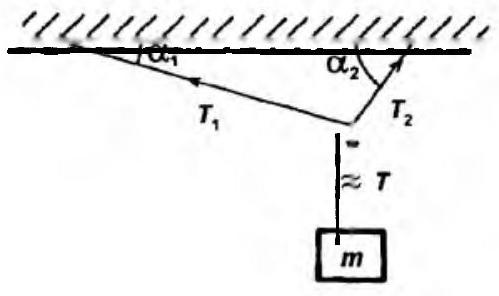
\includegraphics[max width=\textwidth, center]{2025_07_01_5b3ff9fa0d508c8e9f17g-017(1)} Fig. 1.5\\

1.68. Pe un plan înclinat cu unghiul $\alpha$ se aşează un corp de masă $m_{1}$ legat de un al doilea corp de masă $m_{2} \left(m_{2}>m_{1}\right)$ printr-un fir trecut peste un scripete ca în Fig. 1.6. $T$ este forţa de tensiune din firul inextensibil, $\mu$ este coeficientul de frecare dintre corpul cu masa $m_{1}$ şi plan, iar mişcarea fiecărui corp se analizează separat, sensul pozitiv de mişcare fiind indicat de săgețile din figură ($x_{1}, x_{2}$ sunt coordonatele şi $a_{1}, a_{2}$ sunt accelerațiile celor două corpuri). Care din următoarele seturi de relații sunt corecte?\\ A) $\mu m_{1} g \cos \alpha+m_{1} g \sin \alpha-T=m_{1} a_{1}, m_{2} g-T=m_{2} a_{2}, x_{1}+x_{2}=\text{ constant }, a_{1}+a_{2}=0$; B) $\mu m_{1} g \cos \alpha-m_{1} g \sin \alpha-T=m_{1} a_{1}, m_{2} g-T=m_{2} a_{2}, x_{1}+x_{2}=\text{ constant }, a_{1}+a_{2}=0$; C) $\mu m_{1} g \cos \alpha+m_{1} g \sin \alpha-T=m_{1} a_{1}, m_{2} g+T=m_{2} a_{2}, x_{1}+x_{2}=\text{ constant }, a_{1}+a_{2}=0$; D) $\mu m_{1} g \cos \alpha-m_{1} g \sin \alpha-T=m_{1} a_{1}, m_{2} g+T=m_{2} a_{2}, x_{1}+x_{2}=\text{ constant }, a_{1}+a_{2}=0$; E) $\mu m_{1} g \cos \alpha+m_{1} g \sin \alpha+T=m_{1} a_{1}, m_{2} g-T=m_{2} a_{2}, x_{1}+x_{2}=\text{ constant }, a_{1}+a_{2}=0$; F) $\mu m_{1} g \cos \alpha+m_{1} g \sin \alpha-T=m_{1} a_{1}, m_{2} g-T=m_{2} a_{2}, x_{1}+x_{2}=\text{ variabil }, a_{1}+a_{2}=\text{ constant }$.\\ (Vasile Popescu)\\ 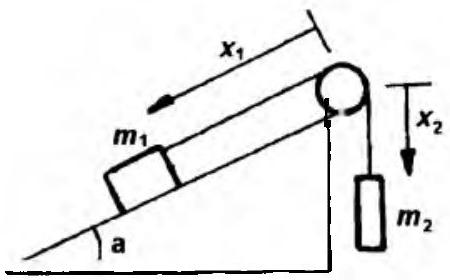
\includegraphics[max width=\textwidth, center]{2025_07_01_5b3ff9fa0d508c8e9f17g-017} Fig. 1.6\\

1.69. Două corpuri cu masele $m_{1}=1 \mathrm{~kg}$ şi $m_{2}=2 \mathrm{~kg}$ sunt legate printr-un fir care trece peste un scripete fixat în vârful comun a două plane înclinate ca în Fig. 1.7. Care este valoarea accelerației fiecărui corp? Se consideră $g=9,8 \mathrm{~m} / \mathrm{s}^{2}$.\\ A) $a_{1}=2,97 \mathrm{~m} / \mathrm{s}^{2}, a_{2}=2,97 \mathrm{~m} / \mathrm{s}^{2}$; B) $a_{1}=4,52 \mathrm{~m} / \mathrm{s}^{2}, a_{2}=2,97 \mathrm{~m} / \mathrm{s}^{2}$; C) $a_{1}=6,28 \mathrm{~m} / \mathrm{s}^{2}, a_{2}=6,28 \mathrm{~m} / \mathrm{s}^{2}$; D) $a_{1}=1,12 \mathrm{~m} / \mathrm{s}^{2}, a_{2}=4,52 \mathrm{~m} / \mathrm{s}^{2}$; E) $a_{1}=19,23 \mathrm{~m} / \mathrm{s}^{2}, a_{2}=2,97 \mathrm{~m} / \mathrm{s}^{2}$; F) $a_{1}=10 \mathrm{~m} / \mathrm{s}^{2}, a_{2}=10 \mathrm{~m} / \mathrm{s}^{2}$.\\ (Vasile Popescu)\\ 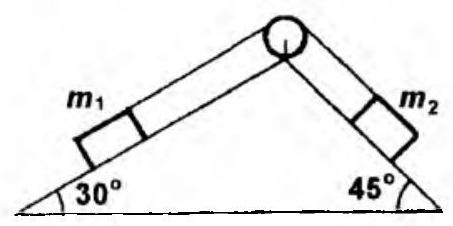
\includegraphics[max width=\textwidth, center]{2025_07_01_5b3ff9fa0d508c8e9f17g-018} Fig. 1.7\\

1.70. Un corp este aruncat de jos în sus pe verticală cu viteza inițială $v_{0}$. Al doilea corp cade liber după $\Delta t$ secunde de la înălțimea $h$. Viteza relativă cu care trec cele două corpuri unul pe lângă altul este:\\ A) $v_{0}-g \Delta t$; B) $v_{0}+g \Delta t$; C) $v_{0}-2 g \Delta t$; D) $h \Delta t+v_{0}-g \Delta t$; E) $v_{0}-g \Delta t+h / \Delta t$; F) $v_{0}-g \Delta t-h / \Delta t$.\\ (Vasile Popescu)\\

1.71. Care este conditia ca un corp aruncat în sus de-a lungul unui plan înclinat să se întoarcă la baza planului ?\\
A) $\operatorname{tg} \alpha=\mu$;\\
B) $\sin \alpha=\mu$;\\
C) $\operatorname{tg} \alpha=1 / \mu$\\
(D) $\operatorname{tg} \alpha>\mu$;\\
E) $\operatorname{tg} \alpha<\mu$; F) $\operatorname{ctg} \alpha>\mu$.\\
(Vasile Popescu)\\
1.72. Un biciclist parcurge distanța $d=314 \mathrm{~m}$ pe o traiectorie sub forma unui Sert de cerc. Să se determine raza cercului.\\
A) 100 m ;\\
B) 314 m ;\\
C) 628 m ;\\
D) 200 m ;\\
E) 50 m ;\\
F) 150 m .\\
(Vasile Popescu)\\
1.73. Un corp cu masa $m=1 \mathrm{~kg}$ este ridicat pe verticală cu accelerația $:=0,19 \mathrm{~m} / \mathrm{s}^{2}$ până la înălțimea $h=10 \mathrm{~m}$. Să se determine lucrul mecanic efectuat $\left.g=9,81 \mathrm{~m} / \mathrm{s}^{2}\right)$.\\
А) 10 J ;\\
B) 150 J ;\\
C) 200 J ;\\
D) 100J;\\
E) 981 J ;\\
F) $9,81 \mathrm{~J}$.\\
(Vasile Popescu)\\
1.74. Pentru a se mişca uniform, un corp în cădere liberă întâmpină din partea zerului o forță de rezistentă de $98,1 \mathrm{~N}$. Să se determine masa corpului $g=9,81 \mathrm{~m} / \mathrm{s}^{2}$ ).\\
A) 2 kg ;\\
B) 5 kg ; (C) 10 kg ;\\
D) $9,81 \mathrm{~kg}$;\\
E) $98,1 \mathrm{~kg}$;\\
F) $0,981 \mathrm{~kg}$.\\
(Vasile Popescu)\\
1.75. O persoană merge prima jumătate din drumul său total cu viteza $v_{1}=6 \mathrm{~km} / \mathrm{h}$, iar cealaltă jumătate cu viteza $v_{2}=4 \mathrm{~km} / \mathrm{h}$. Care este viteza medie a Jersoanei?\\
A) $48 \mathrm{~km} / \mathrm{h}$;\\
B) $9,6 \mathrm{~km} / \mathrm{h}$;\\
C) $5 \mathrm{~km} / \mathrm{h}$; D) $4,8 \mathrm{~km} / \mathrm{h}$;\\
E) $8,4 \mathrm{~km} / \mathrm{h}$;\\
F) $10 \mathrm{~km} / \mathrm{h}$.\\
(Vasile Popescu)\\
1.76. Două corpuri paralelipipedice de mase $m_{1}=2 \mathrm{~kg}$ şi $m_{2}=1 \mathrm{~kg}$ sunt suprapuse pe o masă orizontală fară frecări. Corpul cu masa $m_{1}$ în contact cu masa este împins cu o fortă orizontală $F=6 \mathrm{~N}$. Să se determine accelerația sistemului.\\
A) $1 \mathrm{~m} / \mathrm{s}^{2}$,\\
B) $2 \mathrm{~m} / \mathrm{s}^{2}$;\\
C) $3 \mathrm{~m} / \mathrm{s}^{2}$;\\
D) $0,5 \mathrm{~m} / \mathrm{s}^{2}$;\\
E) $4 \mathrm{~m} / \mathrm{s}^{2}$;\\
F) $1,5 \mathrm{~m} / \mathrm{s}^{2}$.\\
(Vasile Popescu)\\
1.77.* Un corp cu masa $m_{1}=10 \mathrm{~kg}$ se află în repaus. Un alt corp cu masa $m_{2}=2 \mathrm{~kg}$ loveşte primul corp cu viteza $v_{0}=30 \mathrm{~m} / \mathrm{s}$. Să se determine viteza finală a celor două corpuri dacă ciocnirea lor este plastică.\\
A) $5 \mathrm{~m} / \mathrm{s}$;\\
B) $2 \mathrm{~m} / \mathrm{s}$;\\
C) $10 \mathrm{~m} / \mathrm{s}$;\\
D) $1 \mathrm{~m} / \mathrm{s}$;\\
E) $3 \mathrm{~m} / \mathrm{s}$; F) $2,5 \mathrm{~m} / \mathrm{s}$.\\
1.78. Un corp cu energia cinetică inițială $E=24 \mathrm{~J}$ urcă pe un plan înclinat cu unghiul $\alpha=45^{\circ}$ față de orizontală. Coeficientul de frecare între corp şi plan este $\mu=0,2$. Lucrul mecanic al forței de frecare până la oprirea corpului pe plan este:\\
A) 2 J ; B) $\frac{\sqrt{2}}{2} \mathrm{~J}$; C) 3 J ; D) 4 J ; E) $12,2 \mathrm{~J}$; F) $3,6 \mathrm{~J}$.\\
(Mircea Stan)\\
1.79. Un corp cu $m=200 \mathrm{~g}$ cade în $t=3 \mathrm{~s}$ de la înălțimea $h=1,8 \mathrm{~m}$. Forța de rezistență ce acționează asupra corpului este ( $g=9,8 \mathrm{~m} / \mathrm{s}^{2}$ ) :\\
A) $0,88 \mathrm{~N}$; B) $1,08 \mathrm{~N}$; (C) $1,88 \mathrm{~N}$; D) $2,4 \mathrm{~N}$; E) $2,82 \mathrm{~N}$; F) $4,4 \mathrm{~N}$.\\
(Mircea Stan)\\
1.80. O minge este izbită pe verticală de la înălțimea $h=1,8 \mathrm{~m}$, de pământ. În urma ciocnirii, considerate perfect elastice, mingea se înalță la $h^{\prime}=2 \mathrm{~m}$. Viteza inițială a mingii este ( $g=10 \mathrm{~m} / \mathrm{s}^{2}$ ):\\
A) $20 \mathrm{~m} / \mathrm{s}$;\\
B) $10 \mathrm{~m} / \mathrm{s}$;\\
C) $9,8 \mathrm{~m} / \mathrm{s}$;\\
D) $4 \mathrm{~m} / \mathrm{s}$;\\
E) $3,6 \mathrm{~m} / \mathrm{s}$;\\
F) $2 \mathrm{~m} / \mathrm{s}$.\\
(Mircea Stan)\\
1.81. Un om cântărind 70 kg susține o greutate de 16 kg în ajutorul unui fir trecut peste un scripete fix. Care este forța de apăsare normală a omului asupra pământului, dacă firul e înclinat față de verticală cu $60^{\circ} ?\left(g=9,8 \mathrm{~m} / \mathrm{s}^{2}\right)$\\
A) $509,3 \mathrm{~N}$; B) $607,6 \mathrm{~N}$; C) $402,6 \mathrm{~N}$; D) 120 N ; E) $702,6 \mathrm{~N}$; F) 263 N .\\
(Mircea Stan)\\
1.82. Ce putere are un alpinist de 75 kg care se ridică în trei minute la 18 m înălțime? $\left(g=10 \mathrm{~m} / \mathrm{s}^{2}\right)$\\
A) 275 W ; B) 375 ; C) 100 W ; D) 125 W ; E) 75 W ; F) 30 W .\\
(Mircea Stan)\\
1.83. O piatră aruncată vertical în sus revine la punctul de plecare după 4s. Neglijând frecările, înălțimea maximă atinsă de piatră este: $\left(g=10 \mathrm{~m} / \mathrm{s}^{2}\right)$\\
(A) 20 m ; B) 16 m ; C) 10 m ; D) 8 m ; E) 4 m ; F) 2 m .\\
(Mircea Stan)\\
1.84. Un elev care merge cu tramvaiul ține în mână un fir cu plumb. Când zamvaiul frânează brusc, firul se îndepărtează de la verticală cu unghiul $\alpha=30^{\circ}$.\\
Accelerația de frânare a tramvaiului este: ( $g=9,8 \mathrm{~m} / \mathrm{s}^{2}$ )\\
A) $2,65 \mathrm{~m} / \mathrm{s}^{2}$;\\
B) $3,42 \mathrm{~m} / \mathrm{s}^{2}$;\\
C) $4,66 \mathrm{~m} / \mathrm{s}^{2}$;\\
D) $5,66 \mathrm{~m} / \mathrm{s}^{2}$;\\
E) $6,23 \mathrm{~m} / \mathrm{s}^{2}$;\\
F) $6,82 \mathrm{~m} / \mathrm{s}^{2}$.\\
(Mircea Stan)\\
1.85.* Un corp $A$ cu masa $m_{A}=0,8 \mathrm{~kg}$ ciocneşte plastic un corp $B$ cu masa ${ }^{*} \cdot{ }_{B}=1,2 \mathrm{~kg}$ aflat în repaus. În urma ciocnirii cele două corpuri se deplasează ampreună pe un plan orizontal şi parcurg până la oprire $l=4 \mathrm{~cm}$. Coeficientul de Tecare dintre corpuri şi plan fiind $\mu=0,2$ iar $g=10 \mathrm{~m} / \mathrm{s}^{2}$, să se determine viteza aitịală a corpului $A$.\\
A) $1 \mathrm{~m} / \mathrm{s}$;\\
B) $1,5 \mathrm{~m} / \mathrm{s}$;\\
C) $2 \mathrm{~m} / \mathrm{s}$;\\
D) $2,5 \mathrm{~m} / \mathrm{s}$;\\
E) $3 \mathrm{~m} / \mathrm{s}$;\\
F) $3,5 \mathrm{~m} / \mathrm{s}$.\\
(Mircea Stan)\\
1.86. Un mobil este aruncat pe verticală, în sus în câmpul gravitațional terestru $\leqq=9,81 \mathrm{~m} / \mathrm{s}^{2}$ ) cu viteza $v=20 \mathrm{~m} / \mathrm{s}$. Simultan, dintr-un turn vertical de înălțime $\div=40 \mathrm{~m}$ aflat pe aceeaşi verticală cu a primului corp, este aruncat oblic, cu zeeeşi viteză, sub unghiul $\alpha=30^{\circ}$ față de orizontală, un al doilea mobil. Atunci nomentul de timp la care distanța dintre mobile este minimă şi această distanță vor\\
A) $t=2 \mathrm{~s}, d=20 \mathrm{~m}$;\\
B) $t=2 \mathrm{~s}, d=20 \sqrt{3} \mathrm{~m}$;\\
C) $t=1 \mathrm{~s}, d=20 \mathrm{~m}$;\\
D) $t=3 \mathrm{~s}, d=40 \mathrm{~m}$\\
E) $t=1 \mathrm{~s}, d=20 \sqrt{3} \mathrm{~m}$;\\
F) $t=2,5 \mathrm{~s}, d=22 \mathrm{~m}$.\\
(Constantin Roşu)\\
1.87. Un plan înclinat de unghi $\alpha=60^{\circ}$ si masa $m_{1}=3 \mathrm{~kg}$ se poate deplasa :àră frecare pe o suprafață orizontală. El este pus în mişcare sub acțiunea unei forțe rrizontale $F=6 \mathrm{~N}$ dirijate în sensul de mişcare naturală a corpurilor pe plan. Pe ә̧lan se află un corp de masă $m_{2}=0,2 \mathrm{~kg}$ care se poate deplasa cu frecare pe planul aclinat $\left(\mu=0,3 ; g=9,8 \mathrm{~m} / \mathrm{s}^{2}\right)$. Atunci corpul $m_{2}$ va avea față de planul înclinat」rmătoarea dinamică:\\
A) urcă uniform pe plan; B) urcă accelerat cu $a=2 \mathrm{~m} / \mathrm{s}^{2}$;\\
C) coboară accelerat cu $\left.a=5,74 \mathrm{~m} / \mathrm{s}^{2} ; \mathrm{D}\right)$ coboară uniform;\\
E) nu se poate da nici un răspuns cu datele oferite;\\
F) coboară cu accelerația $a=3 \mathrm{~m} / \mathrm{s}^{2}$.\\
1.88. Un pendul matematic este alcătuit dintr-un fir elastic cu lungimea nedeformată $L=2 \mathrm{~m}$ şi constanta elastică $k=10 \mathrm{~N} / \mathrm{m}$. De pendul este agățat un corp cu masa $m=3 \mathrm{~kg}$ care oscilează cu amplitudinea unghiulară $\alpha=45^{\circ}$. Să se calculeze unghiul $\beta$ făcut de fir cu verticala pentru care viteza pendulului este $1 / 2$ din viteza sa maximă?\\
A) $\cos \beta=0,2$;\\
B) $\cos \beta=0,8$;\\
C) $\sin \beta=0,5$;\\
D) $\cos \beta=0,707$;\\
E) $\sin \beta=0,86$; F) $\cos \beta=-0,5$.\\
(Constantin Roşu)\\
1.89.* Un corp de masă $m_{1}$ şi viteză $v$ ciocneşte perfect elastic un corp de masă $m_{2}$ aflat în repaus. După cionire, vitezele corpurilor $m_{1}$ şi $m_{2}$ fac unghiurile $\alpha$ respectiv $\beta$ cu direcția inițialǎ a particulei 1. Raportul energiilor cinetice ale celor 2 particule după cionire este:\\
A) $\frac{E_{c 1}}{E_{c 2}}=\frac{m_{1} \sin ^{2}(\alpha+\beta)}{m_{2} \sin ^{2} \alpha}$;\\
В) $\frac{E_{c 1}}{E_{c 2}}=\frac{m_{2} \sin (\alpha+\beta)}{m_{1} \cos \alpha}$;\\
C) $\frac{E_{c 1}}{E_{c 2}}=\left(\frac{m_{1}}{m_{2}}\right)^{2} \frac{\cos \beta}{\cos ^{2} \alpha}$;\\
D) $\frac{E_{c 1}}{E_{c 2}}=\frac{m_{2} \sin ^{2}(\alpha+\beta)}{\sin ^{2}(\alpha-\beta)}$;\\
Е) $\frac{E_{c 1}}{E_{c 2}}=\frac{m_{2} \sin ^{2} \beta}{m_{1} \sin ^{2} \alpha}$;\\
F) $\frac{E_{c 1}}{E_{c 2}}=\left(\frac{2 m_{1}}{m_{2}}\right)^{2} \frac{\cos ^{2} \beta}{\cos ^{2} \alpha}$.\\
(Constantin Roşu)\\
1.90. Un automobil urcă uniform pe un plan înclinat de unghi mic ( $\sin \alpha=\alpha, \cos \alpha=1$ ) cu viteza $\nu_{1}$. Cu aceeaşi putere a motorului, el va coborî uniform pe planul înclinat cu viteza $v_{2}$. Care este viteza de deplasare pe un plan orizontal, cu putere dublă față de cea folosită pe planul înclinat ?\\
A) $v=\frac{v_{1} \cdot v_{2}}{2 v_{1}+v_{2}}$;\\
B) $v=2 \sqrt{v_{1} \cdot v_{2}}$;\\
C) $v=\frac{4 v_{1} \cdot v_{2}}{v_{1}+v_{2}}$;\\
D) $v=\frac{v_{1} \cdot v_{2}}{v_{1}-v_{2}}$;\\
E) $v=\frac{2 v_{1} \cdot v_{2}}{v_{1}+v_{2}}$;\\
F) $v=\frac{v_{1} \cdot v_{2}}{v_{1}-2 v_{2}}$.\\
1.91. Forța care acționează asupra unui punct material de masă $m$ dintr-un pendul matematic care face unghiul $\alpha$ cu verticala pentru a-l readuce în poziția de echilibru, este:\\
A) $F_{r}=m g \cos \alpha$;\\
B) $F_{r}=m g \sin \alpha$;\\
C) $F_{r}=m g / \cos \alpha$;\\
D) $F_{r}=m g$;\\
E) $F_{r}=m g \operatorname{tg} \alpha$;\\
F) $F_{r}=m g \operatorname{ctg} \alpha$.\\
(Constantin Roşu)\\
1.92. Unui corp aflat pe un plan orizontal cu frecare, $\mu=0,1$ i se imprimă o -.eză inițială $v_{0}=8 \mathrm{~m} / \mathrm{s}$. Cât este spațiul parcurs de corp până la oprire ?

Se dă $g=9,8 \mathrm{~m} / \mathrm{s}^{2}$.\\
А) 23 m ;\\
B) $2,3 \mathrm{~m}$;\\
C) $7,3 \mathrm{~m}$;\\
D) $32,65 \mathrm{~m}$;\\
E) $152,3 \mathrm{~cm}$;\\
F) 10 m .\\
(Răzvan Mitroi)\\
1.93. Mişcarea unui corp este descrisă de ecuația $s=a+b t^{2}$ unde $a=20 \mathrm{~cm}$, $=\bar{b}=4 \mathrm{~cm} / \mathrm{s}^{2}$. Să se afle spațiul parcurs şi viteza corpului dupã timpul $t=2 \mathrm{~s}$.

AD $s=0,36 \mathrm{~m}, v=0,16 \mathrm{~m} / \mathrm{s} ;$ B) $s=6 \mathrm{~m}, v=7,6 \mathrm{~m} ;$ C) $s=3 \mathrm{~m}, v=1,6 \mathrm{~m} / \mathrm{s} ;$\\
D) $s=0,36 \mathrm{~cm}, v=0,16 \mathrm{~cm}$; E) $s=5 \mathrm{~m}, v=4,16 \mathrm{~m}$; F) $s=0,4 \mathrm{~m}, v=0,15 \mathrm{~m} / \mathrm{s}$.\\
(Răzvan Mitroi)\\
1.94. Un corp cade liber de la înălțimea $h=1960 \mathrm{~m}$. Să se determine timpul în :are sunt parcurşi ultimii 60 m . Se dă $g=9,8 \mathrm{~m} / \mathrm{s}^{2}$.\\
A) $0,31 \mathrm{~s}$;\\
B) 13 s ;\\
C) 31 s ;\\
D) 15 s ;\\
E) $5,3 \mathrm{~s}$;\\
F) 12 s .\\
(Răzvan Mitroi)\\
1.95. 0 minge este aruncată orizontal cu viteza $v_{0}=5 \mathrm{~m} / \mathrm{s}$. Să se determine - iteza şi poziția sa după timpul $t=0,5 \mathrm{~s}$. Se dă $g=10 \mathrm{~m} / \mathrm{s}^{2}$.\\
A) $v=5 \sqrt{2} \mathrm{~m} / \mathrm{s}, x=5 \mathrm{~m}, y=1,25 \mathrm{~m}$; B) $v=5 \sqrt{2} \mathrm{~m} / \mathrm{s}, x=5 \mathrm{~m}, y=1,25 \mathrm{~m}$;\\
C) $v=5 \mathrm{~m} / \mathrm{s}, x=5 \mathrm{~m}, y=1,25 \mathrm{~m}$; (D) $v=5 \sqrt{2} \mathrm{~m} / \mathrm{s}, x=2,5 \mathrm{~m}, y=1,25 \mathrm{~m}$;\\
E) $v=5 \sqrt{2} \mathrm{~m} / \mathrm{s}, x=0,5 \mathrm{~m}, y=12,5 \mathrm{~m}$; F) $v=3 \sqrt{2} \mathrm{~m} / \mathrm{s}, x=2,5 \mathrm{~m}, y=1,20 \mathrm{~m}$.\\
(Răzvan Mitroi)\\
1.96. Un biciclist s-a deplasat din punctul $A$ în punctul $B \mathrm{cu}$ viteza $v_{1}=12 \mathrm{~km} / \mathrm{h}$, iar la întoarcerea $\operatorname{din} \mathrm{B}$ în A cu viteza $v_{2}=8 \mathrm{~km} / \mathrm{h}$. Viteza medie a biciclistului este:\\
A) $10 \mathrm{~km} / \mathrm{h}$;\\
B) $9,2 \mathrm{~km} / \mathrm{h}$;\\
C) $20 \mathrm{~km} / \mathrm{h}$;\\
D) $10,5 \mathrm{~km} / \mathrm{h}$;\\
E) $9,6 \mathrm{~km} / \mathrm{h}$;\\
F) $10,6 \mathrm{~km} / \mathrm{h}$.\\
1.97.) Două corpuri de mase $m_{1}=0,2 \mathrm{~kg}$ şi $m_{2}=0,6 \mathrm{~kg}$ sunt legate printr-un fir şi trase în sus cu o fortă $F=8 \mathrm{~N}$. Considerând accelerația gravitațională $g=9,8 \mathrm{~m} / \mathrm{s}^{2}$, tensiunea mecanică din firul de legătură este egală cu:\\
A) 8 N ;\\
В) $7,8 \mathrm{~N}$;\\
C) $6,25 \mathrm{~N}$ ( D ) 6 N ;\\
E) 10 N ; F) $6,7 \mathrm{~N}$.\\
(Ion Belciu)\\
1.98. Un corp este aruncat pe verticală în sus cuviteza $v_{01}=20 \mathrm{~m} / \mathrm{s}$. După ce ajunge la înălțimea maximă, este aruncat în același mod un corp cu viteza inițială $v_{02}=10 \mathrm{~m} / \mathrm{s}$. Cunoscând accelerația gravitațională $g=10 \mathrm{~m} / \mathrm{s}^{2}$, timpul (în raport cu aruncarea celui de-al doilea corp) în care corpurile se întâlnesc este:\\
A) $9,2 \mathrm{~s}$;\\
B) 5 s ;\\
C) 10 s ;\\
D) $2 s$;\\
E) $2,5 \mathrm{~s}$; F) 4 s .\\
(Ion Belciu)\\
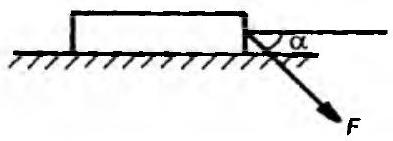
\includegraphics[max width=\textwidth, center]{2025_07_01_5b3ff9fa0d508c8e9f17g-024}

Fig. 1.8.\\
1.99. Un corp de masă $m$, se mişcă uniform pe un plan orizontal sub acțiunea unei forțe $F$ aplicată ca în Fig. 1.8.

Cunoscând accelerația gravitațională $g$, coeficientul de frecare dintre corp şi plan va fi:\\
A) $F+m g$;\\
B) $\frac{m g \sin \alpha}{F}$;\\
C) $\frac{m g+F \cos \alpha}{F \sin \alpha}$;\\
D) $\frac{F \cos \alpha}{m g+F}$\\
(E) $\frac{F \cos \alpha}{m g+F \sin \alpha}$;\\
F) $F \operatorname{tg} \alpha$.\\
(Ion Belciu)\\
1.100. De un tren cu masa $M=110 \mathrm{t}$, care merge rectiliniu şi uniform, se desprinde la un moment dat ultimul vagon de masă $m=10 \mathrm{t}$. Vagonul parcurge o distanță $d=10 \mathrm{~km}$ până se opreşte. Considerând că forțele de frecare sunt proporționale cu greutatea şi că forța de tracțiune a locomotivei trenului a rămas constantă, distanța dintre vagonul oprit şi tren în momentul în care se opreşte vagonul este:\\
A) 32 km ;\\
B) 25 km ;\\
C) 12 km ;\\
D) 24 km ;\\
E) 11 km ;\\
F) $12,5 \mathrm{~km}$.\\
(Ion Belciu)\\
1.101.* Un aviator de masă $m=70 \mathrm{~kg}$ execută un cerc de rază $R=800 \mathrm{~m}$ în plan vertical, cu viteza $v=700 \mathrm{~km} / \mathrm{h}$. Considerând accelerația gravitațională $g=10 \mathrm{~m} / \mathrm{s}^{2}$, forța maximă cu care aviatorul apasă asupra scaunului este:\\
A) 300 N ;\\
B) 7500 N ;\\
C) 4200 N ;\\
D) 3000 N ;\\
E) 5200 N ;\\
F) 700 N .

1.102.*O săgeată de masă $m=0,2 \mathrm{~kg}$ şi cu viteza $v_{1}=15 \mathrm{~m} / \mathrm{s}$ pătrunde într-o sè-í de plastilină de masă $M=0,3 \mathrm{~kg}$ şi care se află în repaus,formând un singur -Energia cinetică a corpului format este:\\
$\therefore$ 20J;B)16,2J;C)8J;D)9J;E)785J;F)5J.\\
(Ion Belciu)\\
1.103)Un corp este aruncat cu viteza inițială $v_{0}$ de-a lungul unui plan înclinat二.三hiul $\alpha=30^{\circ}$ față de un plan orizontal,parcurgând o distanță $l=10 \mathrm{~m}$ ,fără reate.Considerând accelerația gravitațională $g=10 \mathrm{~m} / \mathrm{s}^{2}$ ,valoarea vitezei $v_{0}$ Se égalá cu:\\
A1 $9.8 \mathrm{~m} / \mathrm{s}$ ;\\
B) $7 \mathrm{~m} / \mathrm{s}$ ;\\
C) $12 \mathrm{~m} / \mathrm{s}$ ,(D) $10 \mathrm{~m} / \mathrm{s}$ ;\\
E) $8 \mathrm{~m} / \mathrm{s}$ ;\\
F) $11 \mathrm{~m} / \mathrm{s}$ .\\
(Ion Belciu)\\
1.104.*Un corp cu masa $m_{1}=100 \mathrm{~kg}$ care se mişcă cu viteza $v_{1}=15 \mathrm{~m} / \mathrm{s}$ cuन寸e un alt corp cu masa de 1300 kg ,care inițial stă pe loc.Care este viteza二⿺辶 nă a celor două corpuri,după ciocnirea lor plastică?Care este pierderea de erģie cinetică în procesul de ciocnire?\\
$A 1 u=6,25 \mathrm{~m} / \mathrm{s} ; \Delta E_{c}=67500 \mathrm{~J}$ ;\\
B)$u=6 \mathrm{~m} / \mathrm{s} ; \Delta E_{c}=65000 \mathrm{~J}$ ;\\
()$u=23,47 \mathrm{~km} / \mathrm{h} ; \Delta E_{c}=65 \mathrm{~kJ}$ ;\\
D)$u=6,52 \mathrm{~m} / \mathrm{s} ; \Delta E_{c}=63587 \mathrm{~J}$ ;\\
$E_{1} u=5 \mathrm{~m} / \mathrm{s} ; \Delta E_{c}=64580 \mathrm{~J}$ ;\\
F)$u=5,62 \mathrm{~m} / \mathrm{s}$ ;$\Delta E_{c}=65387 \mathrm{~J}$ .\\
(Elena Slavnicu)\\
1.105.Alegeți relația corectă reprezentând legea lui Hooke a deformărilor ニュー:ce(notații uzuale):\\
A)$F=\frac{E S_{0} \ell}{\Delta \ell_{0}}$ ;\\
В)$\Delta \ell=\frac{F \ell_{0}}{E}$ ;\\
C)$\Delta \ell=E \sigma \quad \ell_{0}$ ;\\
D)$\sigma=\frac{\varepsilon}{E}$ ;\\
E)$F=\frac{E \Delta \ell}{\ell_{0} S_{0}}$ ;\\
F)$E=\frac{F}{\varepsilon S_{0}}$ .\\
(Elena Slavnicu)\\
1.106.Graficul din Fig. 1.9 reprezintă nezndența de timp a vitezei pentru trei mobile nur-erotate 1,2,3.Alegeți afirmația corectă eriertoare la accelerațiile lor:

A)$a_{1}=a_{2}=0$ ,iar $a_{3}$ este pozitivă;\\
B)$a_{2}=0 ; a_{1}$ şi $a_{3}$ sunt pozitive; $a_{1}>a_{3} ;$\\
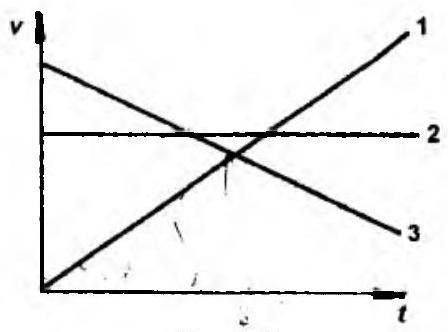
\includegraphics[max width=\textwidth, center]{2025_07_01_5b3ff9fa0d508c8e9f17g-025}

Fig. 1.9\\
C) $a_{1}$ şi $a_{2}$ sunt pozitive, iar $a_{3}$ este negativă;\\
D) $a_{2}=0 ; a_{1}$ şi $a_{3}$ sunt negative; $a_{1}<a_{3}$;\\
E) $a_{2}=0 ; a_{1}$ şi $a_{3}$ sunt pozitive; $a_{1}<a_{3}$;\\
F) $a_{2}=0 ; a_{1}$ este pozitivă, iar $a_{3}$ este negativă.\\
(Elena Slavnicu)\\
1.107. Două corpuri având masele $m_{1}=2 \mathrm{~kg}$ şi $m_{2}=3 \mathrm{~kg}$ sunt legate printr-un fir inextensibil trecut peste un scripete ideal, fixat la marginea unei mese orizontale. Corpul $m_{2}$ atârnă pe verticală, în aer. Între corpul $m_{1}$ şi planul mesei există frecare. Accelerația sistemului este $a=5 \mathrm{~m} / \mathrm{s}^{2}$. Considerând $g=10 \mathrm{~m} / \mathrm{s}^{2}$ şi $\sqrt{2} \cong 1,4$ să se calculeze coeficientul de frecare şi forța care acționează la axul scripetelui.\\
A) 0,$15 ; 24 \mathrm{~N}$;(B) 0,$25 ; 21 \mathrm{~N}$; C) 0,$85 ; 15,5 \mathrm{~N}$;\\
D) 0,$35 ; 18 \mathrm{~N}$; E) 0,$55 ; 17 \mathrm{~N}$; F) nici o variantă nu este corectă.\\
(Nicoleta Eşeanu)\\
1.108. Forța de rupere a unui cablu este cu $40 \%$ mai mare decât tensiunea la care este supus cablul în ridicarea unui corp de masă $m=5 \mathrm{~kg}$ cu accelerația $a=3 \mathrm{~m} / \mathrm{s}^{2}$. Considerând $g=10 \mathrm{~m} / \mathrm{s}^{2}$, să se calculeze masa maximă care poate fi ridicată uniform cu acest cablu.\\
A) $3,45 \mathrm{~kg}$;\\
В) $7,2 \mathrm{~kg}$;\\
C) $7,85 \mathrm{~kg}$,(D) $9,1 \mathrm{~kg}$;\\
E) $10,8 \mathrm{~kg}$;\\
F) $11,7 \mathrm{~kg}$.\\
(Nicoleta Eşeanu)\\
1.109.* Un satelit descrie o orbită circulară în jurul Pământului, la înălțimea $h=15 R$, unde $R \cong 6400 \mathrm{~km}$ este raza Pământului, considerat sferic. Se cunoaşte accelerația gravitațională la suprafața Pământului $g=9,8 \mathrm{~m} / \mathrm{s}^{2}$. Viteza satelitului pe orbită şi perioada mişcării sunt:\\
A) $2,8 \mathrm{~km} / \mathrm{s} ; 25 \mathrm{~h}$; B) $2,5 \mathrm{~km} / \mathrm{s} ; 32,8 \mathrm{~h} ;$ C) $2,8 \sqrt{2} \mathrm{~km} / \mathrm{s} ; 89 \mathrm{~min}$;\\
D) $125,5 \mathrm{~m} / \mathrm{s} ; 85 \mathrm{~h} ;$ E) $1,4 \sqrt{2} \mathrm{~km} / \mathrm{s} ; 114 \mathrm{~h} ;$ F) $1,4 \sqrt{2} \mathrm{~km} / \mathrm{s} ; 127,6 \mathrm{~h}$.\\
(Nicoleta Eşeanu)\\
1.110. Pe un plan înclinat de unghi $\alpha=30^{\circ}$ se află un corp cu masa $m_{1}=600 \mathrm{~g}$, legat printr-un fir inextensibil de un alt corp având masa $m_{2}=900 \mathrm{~g}$. Firul este trecut peste un scripete ideal fixat în vârful planului înclinat, corpul $m_{2}$ atârnând pe verticală, în aer. Coeficientul de frecare dintre corpul $m_{1}$ şi plan este\\
$-=\overline{\overline{3}}$ .iar $g=10 \mathrm{~m} / \mathrm{s}^{2}$ .În aceste condiții accelerația sistemului şi tensiunea エエティ:

$$
\begin{aligned}
& \therefore \mathrm{ms}^{2} 8,1 \mathrm{~N} \text {; B) } 2 \mathrm{~m} / \mathrm{s}^{2} 7,2 \mathrm{~N} \text {; (C) } 3 \mathrm{~m} / \mathrm{s}^{2} 6,3 \mathrm{~N} \text {; } \\
& =-\mathrm{m} \mathrm{~s}^{2} 5,4 \mathrm{~N} \text {; E) } 2 \mathrm{~m} / \mathrm{s}^{2} 10,8 \mathrm{~N} \text {; F) } 3 \mathrm{~m} / \mathrm{s}^{2} 11,7 \mathrm{~N} \text {. }
\end{aligned}
$$

(Nicoleta Eşeanu)\\
1.111.Un corp cu masa $m=800 \mathrm{~g}$ este lansat în sus de-a lungul unui plan $\mathbf{x}$ :-:: u viteza $v_{0}=4 \mathrm{~m} / \mathrm{s}$ .Corpul revine la baza planului înclinat având,în ョ⿱㇒⿺丄丅八土也. 21 respectiv,viteza $v=0,6 v_{0}$ .Lucrul mecanic al forței de frecare de muncise dintre corp şi planul înclinat este:

$$
\therefore-0.58 \mathrm{~J} \text {; B) } 0,85 \mathrm{~J} \text {; C) }-2,8 \mathrm{~J} \text {; D) }-4 \mathrm{~J} \text {; E) }-7,2 \mathrm{~J} \text {; F) } 4,4 \mathrm{~J} \text {. }
$$

(Nicoleta Eşeanu)

1.112.*Un pendul conic este format dintr-un corp punctiform având masa -=$\downarrow$ guspendat printr-un fir de lungime $l=0,4 \mathrm{~m}$ şi masă neglijabilă.Corpul E.:mişcare de rotație uniformă în plan orizontal cu viteza unghiulară $\pm={ }^{-}$ad s .Accelerația gravitațională este $g=9,8 \mathrm{~m} / \mathrm{s}^{2}$ .Să se calculeze unghiul mile:sir şi verticală.\\
A $160^{\circ} ; 0,336 \mathrm{~J} \cdot \mathrm{~s}$ ;\\
B) $45^{\circ} ; 0,6 \mathrm{~J} \cdot \mathrm{~s}$ ;\\
C) $60^{\circ} ; 1,36 \mathrm{~J} \cdot \mathrm{~s}$ ;\\
2. $30^{\circ} ; 0,2 \mathrm{~J} \cdot \mathrm{~s}$ ;\\
Е) $30^{\circ} ; 3,58 \mathrm{~J} \cdot \mathrm{~s}$ ;\\
F) $45^{\circ} ; 0,8 \mathrm{~J} \cdot \mathrm{~s}$ .\\
(Nicoleta Eşeanu)\\
1.113.Două corpuri de mase $m_{1}=200 \mathrm{~g}$ şi $m_{2}=800 \mathrm{~g}$ sunt lansate unul spre $=\dot{1} \equiv l \mathrm{t} \mathrm{cu}$ vitezele $v_{1}=6 \mathrm{~m} / \mathrm{s}$ şi respectiv $v_{2}=2,5 \mathrm{~m} / \mathrm{s}$ .Ciocnirea lor este m:c-mensională şi perfect plastică.Viteza sistemului după ciocnire şi căldura z-.Itată în acest proces sunt:

A) $2,8 \mathrm{~m} / \mathrm{s}$ ,în sensul vitezei $v_{1} ; Q=3,6 \mathrm{~J}$ ;\\
B) $3,2 \mathrm{~m} / \mathrm{s}$ ,in sensul vitezei $v_{1} ; Q=9,8 \mathrm{~J}$ ;\\
C $0.8 \mathrm{~m} / \mathrm{s}$ ,în sensul vitezei $v_{2} ; Q=5,78 \mathrm{~J}$ ;\\
D) $0,4 \mathrm{~m} / \mathrm{s}$ ,în sensul vitezei $v_{2} ; Q=2,56 \mathrm{~J}$ ;\\
E) $5 / 3 \mathrm{~m} / \mathrm{s}$ ,în sensul vitezei $v_{1} ; Q=0,98 \mathrm{~J}$ ;\\
F) $0,8 \mathrm{~m} / \mathrm{s}$ ,în sensul vitezei $v_{1} ; Q=9,8 \mathrm{~J}$ .\\
1.114. O moleculă de masă $m=5 \cdot 10^{-26} \mathrm{~kg}$ loveşte perfect elastic un perete vertical, sub un unghi de $60^{\circ}$ fată de perete. Viteza moleculei înainte de ciocnire este $v=500 \mathrm{~m} / \mathrm{s}$, iar durata ciocnirii este $\Delta t=5 \mathrm{~ms}$. Forța medie cu care peretele acționează asupra moleculei pe durata ciocnirii este:\\
A) $5,6 \cdot 10^{-23} \mathrm{~N}$;\\
B) $3,4 \cdot 10^{-26} \mathrm{~N}$;\\
C) $2,2 \cdot 10^{-22} \mathrm{~N}$;\\
D) $1,86 \cdot 10^{-23} \mathrm{~N}$;\\
E) $8,65 \cdot 10^{-21} \mathrm{~N}$;\\
F) $4,4 \cdot 10^{-22} \mathrm{~N}$.\\
(Nicoleta Eşeanu)\\
1.115.* Un corp punctiform, de masă $m_{1}=200 \mathrm{~g}$, se deplasează cu viteza $v$ pe un plan orizontal şi ciocneşte perfect plastic un alt corp punctiform, de masă $m_{2}=3 m_{1}$. Al doilea corp este legat printr-un resort orizontal, având constanta elastică $k=800 \mathrm{~N} / \mathrm{m}$, de un suport fix. Coeficientul de frecare la alunecare este $\mu=0,225$. Dupã ciocnire sistemul parcurge până la oprire o distantã de 2 cm . Considerând $g=10 \mathrm{~m} / \mathrm{s}^{2}$, să se calculeze viteza primului corp înainte de ciocnire.\\
A) $2,8 \mathrm{~m} / \mathrm{s}$;\\
B) $1,2 \mathrm{~m} / \mathrm{s}$;\\
C) $0,8 \sqrt{5} \mathrm{~m} / \mathrm{s}$;\\
D) $7 \mathrm{~m} / \mathrm{s}$;\\
E) $2,4 \mathrm{~m} / \mathrm{s}$;\\
F) $3,2 \mathrm{~m} / \mathrm{s}$.\\
(Nicoleta Eşeanu)\\
1.116. * Un disc orizontal de rază $R$ se roteşte în jurul axului său vertical. Pe un cerc de rază $r<R$, cu centrul în centrul discului, sunt practicate opt orificii circulare, egale și echidistante, numerotate de la 1 la 8 . De la inălțimea $h=14,7 \mathrm{~m}$, pe verticala orificiului 1, este lăsat să cadă liber un corp punctiform. Cu ce frecvență minimă trebuie să se rotească discul astfel încât corpul să treacă prin orificiul 7 ? Se consideră $g=9,8 \mathrm{~m} / \mathrm{s}^{2}$.\\
A) $\frac{3}{8} \mathrm{rot} / \mathrm{min}$;\\
В) $\frac{\pi}{8} \mathrm{rot} / \mathrm{s}$;\\
C) $\frac{\sqrt{3}}{4} \mathrm{rot} / \mathrm{s}$;\\
D) $\frac{\pi}{\sqrt{3}} \mathrm{rot} / \mathrm{min}$;\\
E) $\frac{\sqrt{3}}{8} \mathrm{rot} / \mathrm{s}$;\\
F) $\frac{\sqrt{3}}{6} \mathrm{rot} / \mathrm{min}$.\\
(Nicoleta Eşeanu)\\
1.117. Un corp este aruncat în sus în câmp gravitațional cu viteza inițialǎ $v_{0}=40 \mathrm{mi} / \mathrm{s}$. Un alt corp, aflat pe aceeaşi verticală, la înălțimea $H=200 \mathrm{~m}$, este lăsat liber în momentul aruncării primului corp. Considerând $g=10 \mathrm{~m} / \mathrm{s}^{2}$, să se calculeze timpul şi înălțimea la care se produce întâlnirea corpurilor.\\
A) $2,5 \mathrm{~s} ; 168,75 \mathrm{~m}$;\\
B) $3 \mathrm{~s} ; 155 \mathrm{~m}$;\\
C) $3,6 \mathrm{~s} ; 135,2 \mathrm{~m}$;\\
D) 4 s ; 120 m ; E) 5 s ; 75 m ; F) 6 s ; $20 . \mathrm{m}$\\
1.118. Două corpuri de masa $m$ sunt legate printr-un fir inextensibil care este z:ut peste un scripete fix. Pe corpul din partea stânga se aşează o greutate de -:=1 $m_{0}$. Accelerația sistemului are expresia:\\
A) $\frac{2 m g}{m_{0}+m}$; B) $\frac{m_{0} g}{m+2 m_{0}}$; C) $\frac{m g}{2 m+m_{0}}$;\\
D) $\frac{m_{0} g}{2 m+m_{0}}$; E) $\frac{m g}{2 m_{0}+m}$; F) $\frac{2 m_{0} g}{m_{0}+m}$.\\
(Daniela Buzatu)\\
1.11. O şalupă se deplasează pe un râu din punctul A spre punctul B în Zul $t_{1}$, şi înapoi în timpul $t_{2}$. Cât timp îi este necesar şalupei să parcurgă kèeaşi distanță AB cu motorul oprit?\\
A) $\frac{2 t_{1} t_{2}}{t_{1}+t_{2}}$;\\
B) $\frac{2 t_{1} t_{2}}{2 t_{2}-t_{1}}$;\\
C) $\frac{2 t_{1} t_{2}}{t_{2}-t_{1}}$;\\
D) $\frac{t_{1} t_{2}}{t_{1}+t_{2}}$;\\
E) $\frac{2 t_{1} t_{2}}{2 t_{1}-t_{2}}$;\\
F) $\frac{t_{1} t_{2}}{t_{2}-t_{1}}$.\\
(Daniela Buzatu)\\
1.120. Viteza medie a unui călātor care parcurge primul sfert din timp cu -zza $v_{1}=7 \mathrm{~km} / \mathrm{h}$, iar restul timpului cu viteza $v_{2}=4 \mathrm{~km} / \mathrm{h}$ şi viteza medie a unui 1: zălător care parcurge primul sfert din drum cu viteza $v_{1}=7 \mathrm{~km} / \mathrm{h}$, iar restul \_\_mului cu viteza $v_{2}=4 \mathrm{~km} / \mathrm{h}$, sunt:\\
A) $4,25 \mathrm{~km} / \mathrm{h} ; 8,84 \mathrm{~km} / \mathrm{h} ; \mathrm{B}) 4,75 \mathrm{~km} / \mathrm{h} ; 4,48 \mathrm{~km} / \mathrm{h}$;\\
C) $5,75 \mathrm{~km} / \mathrm{h} ; 4,88 \mathrm{~km} / \mathrm{h}$; D) $5,57 \mathrm{~km} / \mathrm{h} ; 8,48 \mathrm{~km} / \mathrm{h}$;\\
E) $7,75 \mathrm{~km} / \mathrm{h} ; 4,84 \mathrm{~km} / \mathrm{h} ; \mathrm{F}) 7,25 \mathrm{~km} / \mathrm{h} ; 8,88 \mathrm{~km} / \mathrm{h}$.\\
(Daniela Buzatu)\\
1.121. O minge de masă $m=0,2 \mathrm{~kg}$ cade de la înălțimea de 1 m cu accelerația $==8 \mathrm{~m} / \mathrm{s}^{2}$. Variația impulsului mingii este:\\
A) $0,5657 \mathrm{~kg} \mathrm{~m} / \mathrm{s}$; (B) $0,8 \mathrm{~kg} \mathrm{~m} / \mathrm{s}$; C) $0,4 \mathrm{~kg} \mathrm{~m} / \mathrm{s}$;\\
D) $2,8284 \mathrm{~kg} \mathrm{~m} / \mathrm{s}$; E) $0,2828 \mathrm{~kg} \mathrm{~m} / \mathrm{s}$; F) $0,8854 \mathrm{~kg} \mathrm{~m} / \mathrm{s}$.\\
(Daniela Buzatu)\\
1.122. Un automobil se deplasează cu viteza $v=72 \mathrm{~km} / \mathrm{h}$ pe un podeț ce are spectul unui arc de cerc. În punctul superior al podețului forța sa de apăsare - ormală se miç̧orează de două ori ( $g=10 \mathrm{~m} / \mathrm{s}^{2}$ ). Raza podețului este:\\
A) 40 m ;\\
B) $14,4 \mathrm{~m}$;\\
C) 80 m ;\\
D) 4 m ;\\
E) 8 m ;\\
F) 72 m .\\
1.123. O piatră de masă $m=5 \mathrm{~kg}$ este aruncată vertical în jos de la înălțimea $h=5 \mathrm{~m} \mathrm{cu} \mathrm{viteza} \mathrm{inițială} v_{0}=2 \mathrm{~m} / \mathrm{s}$. Înainte de impactul cu Pământul, viteza pietrei era $v=4 \mathrm{~m} / \mathrm{s}$. Lucrul mecanic al forței de rezistență a aerului este:\\
A) +220 J ;\\
B) -220 J ;\\
C) -190 J ;\\
D) +190 J ;\\
E) +470 J ;\\
F) -470 J .\\
(Daniela Buzatu)\\
1.124. Pentru a menține constantă viteza unei sănii pe un drum orizontal trebuie să actionăm cu o forță $F_{1}=120 \mathrm{~N}$ sub un unghi $\alpha_{1}=60^{\circ}$ fată de orizontală, sau cu o forță $F_{2}=50 \sqrt{3} \mathrm{~N}$ sub un unghi $\alpha_{2}=30^{\circ}\left(g=10 \mathrm{~m} / \mathrm{s}^{2}\right)$. Între sanie şi drum există frecare. Masa saniei are valoarea:\\
A) $60 / 7 \mathrm{~kg},(\mathrm{~B}) 20 \sqrt{3} \mathrm{~kg}$;\\
C) $7 / 60 \mathrm{~kg}$;\\
D) $40 \sqrt{3} \mathrm{~kg}$;\\
E) $10 \sqrt{3} \mathrm{~kg}$;\\
F) $60 \sqrt{3} \mathrm{~kg}$.\\
(Daniela Buzatu)\\
1.125. Un proiectil cu masa $m=5 \mathrm{~kg}$ şi cu viteza $v_{0}=300 \mathrm{~m} / \mathrm{s}$ intră într-un strat de zăpadă de lungime $l=10 \mathrm{~km}$. Stratul absoarbe prin frecare o cantitate de căldură $Q=200 \mathrm{~kJ}$. Viteza la ieşirea din strat, accelerația şi timpul în care proiectilul străbate stratul de zăpadă sunt:\\
A) $100 \mathrm{~m} / \mathrm{s} ;-4 \mathrm{~m} / \mathrm{s}^{2} ; 50 \mathrm{~s} ;$ B) $200 \mathrm{~m} / \mathrm{s} ;-2 \mathrm{~m} / \mathrm{s}^{2} ; 25 \mathrm{~s}$;\\
C) $200 \mathrm{~m} / \mathrm{s} ;-2 \mathrm{~m} / \mathrm{s}^{2} ; 50 \mathrm{~s}$;\\
D) $100 \mathrm{~m} / \mathrm{s} ;+4 \mathrm{~m} / \mathrm{s}^{2} ; 50 \mathrm{~s}$;\\
D) $200 \mathrm{~m} / \mathrm{s} ;+2 \mathrm{~m} / \mathrm{s}^{2} ; 25 \mathrm{~s}$;\\
F) $100 \mathrm{~m} / \mathrm{s} ;-4 \mathrm{~m} / \mathrm{s}^{2} ; 25 \mathrm{~s}$.\\
(Daniela Buzatu)\\
1.126. Un corp aruncat orizontal din vârful unui plan înclinat spre bază cade péplan-la distanta $l=30 \mathrm{~m}$ de vârf. Cunoscând înclinația planului față de $\mathrm{O} x$, $\alpha=30^{\circ}$ şi $g=10 \mathrm{~m} \cdot \mathrm{~s}^{-2}$, viteza inițială $v_{0}$ cu care este aruncat corpul are valoarea:\\
A) $10 \mathrm{~m} \cdot \mathrm{~s}^{-1}$;\\
B) $12 \mathrm{~m} \cdot \mathrm{~s}^{-1}$;\\
C) $15 \mathrm{~m} \cdot \mathrm{~s}^{-1}$;\\
D) $0,1 \mathrm{~m} \cdot \mathrm{~s}^{-1}$;\\
E) $1,2 \mathrm{~m} \cdot \mathrm{~s}^{-1}$;\\
F) $1,5 \mathrm{~m} \cdot \mathrm{~s}^{-1}$.\\
(Ilie Ivanov)\\
1.127. Două corpuri de masă $M$, respectiv $m(M>m)$ sunt legate între ele printr-un fir de legătură de greutate neglijabilă şi se află pe o suprafață orizontală aşa cum arată Fig. 1.10.\\
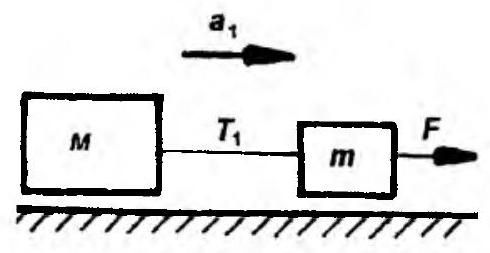
\includegraphics[max width=\textwidth, center]{2025_07_01_5b3ff9fa0d508c8e9f17g-031(1)}

Caz 1\\
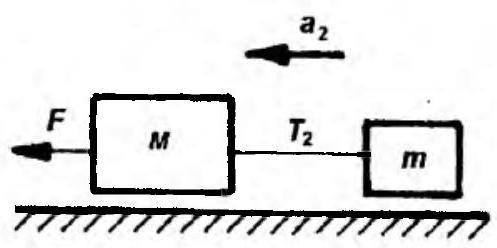
\includegraphics[max width=\textwidth, center]{2025_07_01_5b3ff9fa0d508c8e9f17g-031}

Caz 2

Fig. 1.10\\
Dacă sistemul este acționat de o forță orizontală $F$ ce acționează asupra二rpului de masă $m$ ,sistemul se va mişca accelerat cu accelerația $a_{1}$ ,tensiunea în Fal de legătură fiind $T_{1}$(caz 1).Dacă însă aceeaşi forță actionează asupra二rpului de masă $M$ ,accelerația sistemului va fí $a_{2}$ şi tensiunea $T_{2}$(caz 2).În $x=$ ste condiții:\\
A)$a_{1}=a_{2} ; T_{1}>T_{2}$ ;\\
B)$a_{1}>a_{2} ; T_{1}<T_{2}$ ;\\
C)$a_{1}<a_{2} ; T_{1}>T_{2}$ ;\\
D)$a_{1}<a_{2} ; T_{1}<T_{2}$ ;\\
E)$a_{1}>a_{2} ; T_{1}=T_{2}$ ;\\
F)$a_{1}=a_{2} ; T_{1}=T_{2}$ .\\
(Ilie Ivanov)\\
1.128.Două resorturi de constante elastice $k_{1}$ ,respectiv $k_{2}$ ,legate în serie $\therefore$ :ンin un corp de masă $M$ .Raportul între energiile potentiale ale resorturilor este:\\
A)$\frac{E_{1}}{E_{2}}=\frac{k_{1}}{k_{2}}$ ;\\
B)$\frac{E_{1}}{E_{2}}=\frac{k_{2}}{k_{1}}$ ;\\
C)$\frac{E_{1}}{E_{2}}=\frac{k_{1}^{2}}{k_{2}^{2}}$ ;\\
D)$\frac{E_{1}}{E_{2}}=\frac{k_{2}^{2}}{k_{1}^{2}}$ ;\\
E)$\frac{E_{1}}{E_{2}}=\frac{k_{1}+k_{2}}{k_{1}-k_{2}}$ ;\\
F)$\frac{E_{1}}{E_{2}}=\frac{k_{1}-k_{2}}{k_{1}+k_{2}}$ .\\
(Ilie Ivanov)\\
1.129.Un patinator de masă $M=80 \mathrm{~kg}$ ține în mână o bilă de masă $m=8 \mathrm{~kg}$ ::ce află în repaus pe gheață.La un moment dat aruncă bila înainte cu viteza $=10 \mathrm{~m} \cdot \mathrm{~s}^{-1}$ .Cunoscând $g=10 \mathrm{~m} \cdot \mathrm{~s}^{-2}$ şi coeficientul de frecare cu gheața _=0,001,spațiul parcurs de patinator în urma acestei operații,este:\\
A) 50 m ;\\
B) 60 m ;\\
C) 70 m ;\\
D) 5 m ;\\
E) $0,6 \mathrm{~m}$ ;\\
F) $4,5 \mathrm{~m}$ .\\
(Ilie Ivanov)\\
1.130.Viteza unui mobil este dată de relația $v=m+n t^{2}$ ,unde $m=16 \mathrm{~cm} / \mathrm{s}$ $\pm n=0,8 \mathrm{~cm} / \mathrm{s}^{2}$ .Să se afle viteza şi accelerația instantanee la momentul $t=5 \mathrm{~s}$ .\\
А)$v=1 \mathrm{~m} / \mathrm{s}, a=0,8 \mathrm{~m} / \mathrm{s}^{2}$ ;\\
B)$v=2 \mathrm{~m} / \mathrm{s}, a=1 \mathrm{~m} / \mathrm{s}^{2}$ ;\\
C) $v=0,18 \mathrm{~m} / \mathrm{s}, a=0,08 \mathrm{~m} / \mathrm{s}^{2}$;\\
D) $v=8 \mathrm{~m} / \mathrm{s}, a=0,08 \mathrm{~m} / \mathrm{s}^{2}$;\\
E) $v=0,8 \mathrm{~m} / \mathrm{s}, a=1,8 \mathrm{~m} / \mathrm{s}^{2}$;\\
F) $v=0,7 \mathrm{~m} / \mathrm{s} ; a=1,5 \mathrm{~m} / \mathrm{s}^{2}$.\\
(Ileana Creangă)\\
1.131. O forță orizontală constantă de 45 N acționează asupra unui corp aflat pe un plan orizontal neted. Corpul porneşte din repaus şi parcurge 75 m în 5 s , după care forța îşi încetează acțiunea. Să se determine spațiul parcurs de corp în următoarele 5 s .\\
A) 15 m ;\\
B) 5 m ;\\
C) 120 m ;\\
D) 130 m (E) 150 m ;\\
F) 100 m .\\
(Ileana Creangă)\\
1.132. Un electron de masă $m=9 \cdot 10^{-31} \mathrm{~kg}$ părǎseşte catodul unui tub electronic cu viteza inițială zero şi se deplasează rectiliniu până la anod, aflat la distanța de 1 cm . Electronul ajunge la anod cu viteaza de $6 \cdot 10^{6} \mathrm{~m} / \mathrm{s}$. Cât este forța de accelerație care acționează asupra electronului ?\\
A) $1,62 \cdot 10^{-15} \mathrm{~N}$;\\
B) $1,62 \mathrm{~N}$;\\
C) $1 \cdot 10^{-14} \mathrm{~N}$;\\
D) $12 \cdot 10^{-10} \mathrm{~N}$;\\
E) $6,5 \cdot 10^{-15}$\\
N ;\\
F) $5,5 \cdot 10^{-14} \mathrm{~N}$.\\
(Ileana Creangă)\\
1.133. Un corp de masă $m=5 \mathrm{~kg}$ este susținut de o coardă şi este tras în sus cu o accelerație de $2 \mathrm{~m} / \mathrm{s}^{2}$. După $t_{1}=2 \mathrm{~s}$ tensiunea din coardă se reduce la 49 N . Să se afle spațiul parcurs de corp după $t_{2}=5 \mathrm{~s}$ de la pornire ( $\mathrm{g}=9,8 \mathrm{~m} / \mathrm{s}^{2}$ )\\
A) 5 m ;\\
B) 7 m ;\\
(e) 16 m ;\\
D) 10 m ;\\
E) 25 m ; F) 12 m .\\
(Ileana Creangă)\\
f.134. Un avion zboară orizontal cu viteza de $90 \mathrm{~m} / \mathrm{s}$, şi lansează un obiect de la înălțimea de 1900 m . Să se determine componentele vitezei obiectului în mometul impactului cu Pământul. Se dă $g=10 \mathrm{~m} / \mathrm{s}^{2}$.\\
A) $9 \mathrm{~m} / \mathrm{s}$ şi $194,9 \mathrm{~m} / \mathrm{s}$;\\
B) $900 \mathrm{~m} / \mathrm{s}$ şi $19 \mathrm{~m} / \mathrm{s}$;\\
C) $100 \mathrm{~m} / \mathrm{s}$ şi $250 \mathrm{~m} / \mathrm{s}$;\\
(D) $90 \mathrm{~m} / \mathrm{s}$ şi $194,9 \mathrm{~m} / \mathrm{s}$;\\
E) $0 \mathrm{~m} / \mathrm{s}$ şi $100 \mathrm{~m} / \mathrm{s}$;\\
F) $85 \mathrm{~m} / \mathrm{s}$ şi $190,5 \mathrm{~m} / \mathrm{s}$.\\
(Ileana Creangă)\\
1.135. Un corp cu masa $m=2 \mathrm{~kg}$ este lăsat să cadă liber de la înălțimea $h=50 \mathrm{~m}$. Se cere valoarea energiei mecanice pe care o are corpul la înălțimea $h_{1}=10 \mathrm{~m}$. Se dă $g=10 \mathrm{~m} / \mathrm{s}^{2}$.\\
A) 800 J ;\\
B) 2500 J ;\\
C) 3000 J ;\\
D) 1000 J ;\\
E) 200 J ;\\
F) 900 J .

1.136.De tavanul unui lift este suspendat un dinamometru de care atârnă un $\therefore$ cu masa $m=2 \mathrm{~kg}$ .Ce forţă indică dinamometrul dacă liftul urcă cu цこelerația $a=1,2 \mathrm{~m} / \mathrm{s}^{2}$(se consideră $g=9,8 \mathrm{~m} / \mathrm{s}^{2}$ ).\\
A) 22 N ;\\
B) 11 N ;\\
C) $8,6 \mathrm{~N}$ ;\\
D) $2,4 \mathrm{~N}$ ;\\
E) $17,2 \mathrm{~N}$ ;\\
F) 100 N .\\
(Gabriela Tiriba)\\
1.137.Pe o masă orizontală netedã fără二esäri sunt aşezate alături doua corpuri a-alelipipedice de mase $m_{1}=8 \mathrm{~kg}$ şi $\square_{=}^{=}=2 \mathrm{~kg}$(fig.1.11).Sistemul astfel format ne impins(dinspre $m_{1}$ )cu o forță orizontală $\overline{ }=50 \mathrm{~N}$ .Cu ce forță $f$ corpul $m_{1}$ împinge\\
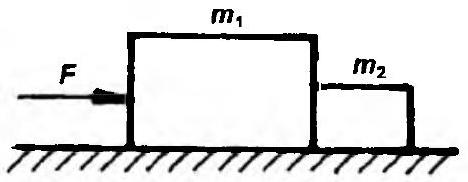
\includegraphics[max width=\textwidth, center]{2025_07_01_5b3ff9fa0d508c8e9f17g-033}

Fig. 1.11 :orpul $m_{2}$ ?

A) 2 N ;B) 25 N ;C) 120 N ;D) 10 N ;E) 16 N ;F) 150 N .\\
(Gabriela Tiriba)\\
1.138.Un corp se mişcă uniform accelerat parcurgând distanta $d=120 \mathrm{~m}$ . Z-ima jumătate de drum o parcurge în timpul $t_{1}=12 \mathrm{~s}$ ,iar cea de-a doua jumătate $=$ aimpul $t_{2}=8 \mathrm{~s}$ .Să se afle accelerația corpului.\\
A) $1 \mathrm{~m} / \mathrm{s}$ ;\\
B) $0,25 \mathrm{~m} / \mathrm{s}^{2}$ ;\\
C) $0,2 \mathrm{~m} / \mathrm{s}$ ;\\
D) $1,2 \mathrm{~m} / \mathrm{s}^{2}$ ;\\
E) $4 \mathrm{~m} / \mathrm{s}^{2}$ ;\\
F) $8 \mathrm{~m} / \mathrm{s}^{2}$ .\\
(Gabriela Tiriba)\\
1.139.Un corp este aruncat vertical în sus și revine pe pământ după un timp $:=2 \mathrm{~s}$ .Sã se afle înălțimea la care s-a ridicat corpul $\left(g=9,8 \mathrm{~m} / \mathrm{s}^{2}\right)$ .\\
А) $19,6 \mathrm{~m}$ ;\\
B) $9,8 \mathrm{~m}$ ;\\
C) $39,2 \mathrm{~m}$ ;\\
D) $4,9 \mathrm{~m}$ ;\\
E) $29,4 \mathrm{~m}$ ;\\
F) 16 m .\\
(Gabriela Tiriba)\\
1.140.Pentru a mentine în echilibru un corp pe un plan înclinat de unghi $a=45^{\circ}$ ,trebuie aplicată corpului o fortă minimă normală pe plan de $n=2$ ori nai mare decât forța minimă orizontală.Să se calculeze coeficientul de frecare tintre corp şi plan.\\
A)$\frac{1}{7}$ ;\\
B)$\frac{1}{2}$ ;\\
C)$\frac{1}{\sqrt{2}}$ ;\\
D)$\frac{\sqrt{2}+1}{7+\sqrt{2}}$ ;\\
E)$\frac{\sqrt{3}}{2}$ ;\\
F)$\frac{1}{2 \sqrt{2}-1}$ .\\
1.141. Un automobil face un viraj de rază $R=50 \mathrm{~m}$ cu viteza $v=36 \mathrm{~km} / \mathrm{h}$. Sã se afle coeficientul de frecare la alunecare minim pentru ca automobilul să nu alunece lateral $\left(g=9,8 \mathrm{~m} / \mathrm{s}^{2}\right)$.\\
А) 0,1 ;\\
B) 0,03 ;\\
C) 0,2 ;\\
D) 0,5 ;\\
Е) 0,9 ;\\
F) 0,04 .\\
(Gabriela Tiriba)\\
1.142. Un motor are puterea $P=98 \mathrm{~kW}$. Motorul este folosit pentru a ridica un corp cu masa $m=500 \mathrm{~kg}$ la o înălțime $h=18 \mathrm{~m}$. În cât timp va ridica motorul corpul respectiv?\\
A) 5 s ;\\
B) 90 s ;\\
C) $0,9 \mathrm{~s}$;\\
D) 1 min ;\\
E) 18 s ; F) 15 min .\\
(Gabriela Tiriba)\\
1.143. Ce fortă constantă de frânare trebuie aplicatã unui tun de masă $m=400$ tone care se mişcă cu viteza $v_{0}=36 \mathrm{~km} / \mathrm{h}$, pentru a-l opri în timp de 20 s ?\\
А) 150 N ;\\
B) 36 N ;\\
(C) 200 kN ;\\
D) 300 kN ;\\
E) 10 N ;\\
F) 3 kN .\\
(Gabriela Tiriba)\\
1.144. Un mobil se găseşte la momentul $t=0$ în punctul de coordonate $(2,0)$. Mobilul se mişcã în lungul axei Ox conform legii de mişcare $x(t)=4 t^{2}+3 t+2$. La momentul $t=3 \mathrm{~s}$ de la începutul mişcării, viteza mobilului este:\\
A) $11 \mathrm{~m} / \mathrm{s}$;\\
(B) $27 \mathrm{~m} / \mathrm{s}$;\\
C) $13 \mathrm{~m} / \mathrm{s}$;\\
D) $17 \mathrm{~m} / \mathrm{s}$;\\
E) $19 \mathrm{~m} / \mathrm{s}$;\\
F) $37 \mathrm{~m} / \mathrm{s}$.\\
(Mihai Cristea)\\
1.145. Un corp este lansat cu aceeași viteză, o dată pe un plan înclinat de unghi $\alpha$ şi altă dată pe un plan orizontal, ambele caracterizate de acelaşi coeficient de frecare. atiind că obiectul parcurge aceeaşi distanță până la oprire pe ambele plane, să se calculeze unghiul de frecare.\\
A) $\varphi=\alpha$;\\
B) $\varphi=\frac{\alpha}{2}$;\\
C) $\varphi=\frac{\pi-\alpha}{6}$;\\
D) $\varphi=\frac{\pi}{4}$;\\
E) $\varphi=\frac{\pi-\alpha}{2}$;\\
F) $\varphi=\frac{2 \pi-\alpha}{4}$

1.146.Un corp este aruncat sub unghiul $\alpha$ în câmp gravitațional.Să se rézascā unghiul $\beta$ facut de viteză cu orizontala atunci când energia cinetică a arcului devine de $n$ ori mai mică decât energia cinetică inițială.\\
A) $\operatorname{tg} \beta=\sqrt{1+\frac{1}{n \cos ^{2} \alpha}}$ ;\\
B) $\sin \beta=\frac{1}{\sqrt{n}}$ ;\\
C) $\cos \beta=\sqrt{n} \cos \alpha$ ;\\
D) $\operatorname{tg} \beta=\sqrt{1+\frac{1}{n \sin ^{2} \alpha}}$ ;\\
E) $\sin \beta=\frac{1}{n}$ ;\\
F) $\cos \beta=\sqrt{n} \sin \alpha$ .\\
(Mihai Cristea)

1.147 Un corp cu masa $m=\mathrm{lkg}$ pleacă din Zeaus şi se mişcă fără frecare sub acțiunea forței -rezentată în Fig.1.12.Când mobilul ajunge în ᄀ二⿺辶rul $x=8 \mathrm{~m}$ ,viteza lui va fi :\\
A) $4 \mathrm{~m} / \mathrm{s}$ ;\\
B) $18 \mathrm{~m} / \mathrm{s}$ ;\\
C) $36 \mathrm{~m} / \mathrm{s}$ ;\\
D) $0 \mathrm{~m} / \mathrm{s}$ ;E) (r.: F ) $9 \mathrm{~m} / \mathrm{s}$ .\\
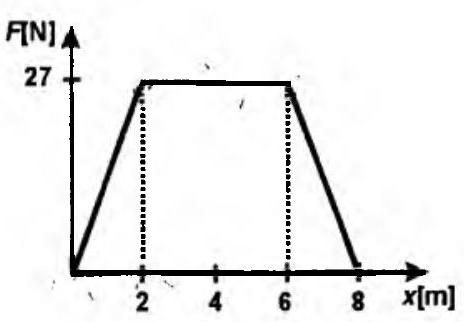
\includegraphics[max width=\textwidth, center]{2025_07_01_5b3ff9fa0d508c8e9f17g-035}

Fig. 1.12\\
(Mihai Cristea)\\
1.148.*Două corpuri de mase $m_{1}$ şi $m_{2}=n \cdot m_{1}(n>1)$(Fig.1.13)alunecă mri frecare pe un profil cilindric de zi:$R$ ,de la nivelul centrului :-ndrului.În urma ciocnirii plastice a **două corpuri,fracțiunea din ęęgia potențială inițială transformată r.:äldură este:\\
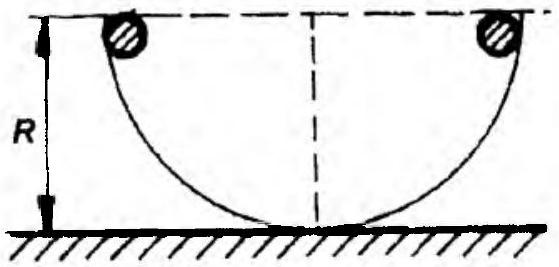
\includegraphics[max width=\textwidth, center]{2025_07_01_5b3ff9fa0d508c8e9f17g-035(1)}

Fig. 1.13\\
A)$\frac{n}{n+1}$ ;\\
В)$\left(\frac{n}{n+1}\right)^{2}$ ;\\
C)$\frac{n-1}{n+1}$ ;\\
D)$\left(\frac{n-1}{n+1}\right)^{2}$ ;\\
E)$\frac{2 n}{n^{2}+1}$ ;\\
F)$\frac{4 n}{(n+1)^{2}}$ .\\
(Mihai Cristea)

1.149.Un corp masiv de masă $M$ este agățat de un fir inextensibil şi atârnă la :Sistantă $h_{1}$ de nivelul solului.Dacă se aruncă exact sub el,de la înălțimea $h_{2}$千а் de sol un corp de masă $m$ ,acesta,în urma ciocnirii plastice,va ridica sistemul $\therefore$ :or două corpuri pe o distanță $x$ .Cunoscând viteza inițială $v_{0}$ cu care se aruncă\\
corpul de masă $m$, să se determine cu cât se va modifica poziția corpului atârnat, înainte să cadă din nou.\\
A) $x=\left(\frac{m}{m+M}\right)^{2}\left(\frac{v_{0}^{2}}{2 g}-h_{1}+h_{2}\right) ;$ B) $x=\left(\frac{m}{m+M}\right) \cdot\left(\frac{v_{0}^{2}}{2 g}-h_{1}+h_{2}\right) ;$\\
C) $x=\left(\frac{m}{m+M}\right) \cdot\left(\frac{v_{0}^{2}}{2 g}-h_{1}-h_{2}\right)$; D) $x=\left(\frac{m}{m+M}\right) \cdot\left(\frac{v_{0}^{2}}{2 g}+h_{1}-h_{2}\right)$;\\
E) $x=\left(\frac{m}{m+M}\right)^{2}\left(\frac{v_{0}^{2}}{2 g}+h_{1}-h_{2}\right)$; F) $x=\left(\frac{m}{m+M}\right)^{2}\left(\frac{v_{0}^{2}}{2 g}-h_{1}-h_{2}\right)$.\\
(Cristina Stan)\\
1.150. De la fereastra unui bloc turn, aflată la înălțimea de 25 m față de sol, un copil lasă să cadă o castană. După o secundă, el aruncă cu viteza inițială de $15 \mathrm{~m} / \mathrm{s}$ o a doua castană. Se întâlnesc cele două castane în drumul lor spre sol? La ce distantă față de fereastră? $\left(\mathrm{g}=10 \mathrm{~m} / \mathrm{s}^{2}\right)$\\
A) Da, $d=18,4 \mathrm{~m}$;\\
B) $\mathrm{Nu}, d=15,2 \mathrm{~m}$;\\
C) Da, $d=6,6 \mathrm{~m}$;\\
D) Da, $d=4,9 \mathrm{~m}$;\\
E) Da, $d=19,9 \mathrm{~m}$;\\
F) $\mathrm{Nu}, d=6,6 \mathrm{~m}$.\\
(Cristina Stan)\\
1.151. Un corp cu masa $m=10 \mathrm{~kg}$ este împins cu o fortẵ orizontală de-a lungul unui plan înclinat care face unghiul $\alpha=45^{\circ}$ față de orizontală. Ce mărime trebuie să aibă această fortă pentru a produce o accelerație $a=1 / \sqrt{2} \mathrm{~m} / \mathrm{s}^{2}$ ştiind că valoarea coeficientului de frecare dintre corp şi planul înclinat este $\mu=0,2$ ? Se va considera accelerația gravitațională $g=10 \mathrm{~m} / \mathrm{s}^{2}$ ?\\
А) 75 N ;\\
B) 100 N ;\\
C) 450 N ;\\
D) $162,5 \mathrm{~N}$;\\
Е) $55,7 \mathrm{~N}$;\\
F) 90 N .\\
(Cristina Stan)\\
1.152. O forță care acționează asupra unui obiect cu masa $m_{1}$ îi imprimă acestuia o accelerație $a_{1}$. Aceeaşi forță acționând asupra unei mase diferite, $m_{2}$, îi imprimă accelerația $a_{2}=2 a_{1}$. Dacă se lipesc cele două mase, ce accelerație va avea sistemul ?\\
A) $3 a_{1}$;\\
B) $\frac{1}{3} a_{1}$;\\
C) $\frac{3}{2} a_{1}$;\\
(Б) $\frac{2}{3} a_{1}$;\\
E) $\frac{4}{3} a_{1}$;\\
F) $\frac{5}{3} a_{1}$.

1.153.*Un automobil cu masa $m=800 \mathrm{~kg}$ staționează pe partea dreaptă a r.ai drum national.Un autocamion cu masa $M=1200 \mathrm{~kg}$ venind cu viteza $={ }^{-} 2 \mathrm{~km} / \mathrm{h}$ dintr-o curbă,nu îl observă în timp util astfel că se produce o z.ziziune în urma căreia ambele maşini rămân lipite.Pe ce distantặ se deplasează $\therefore$-:rmul format din cele două maşini dacă coeficientul de frecare este $\mu=0,2$ ?Se -nsideră accelerația gravitațională $g=10 \mathrm{~m} / \mathrm{s}^{2}$ .\\
A) 55 m ;\\
B) 122 m ;\\
C) $3,6 \mathrm{~m}$ ;\\
D) $46,7 \mathrm{~m}$ ;\\
E) 36 m ;\\
F) 32 m .\\
(Cristina Stan)\\
1.154.Două bile se deplasează una spre cealaltă,viteza bilei mai grele fiind je วatru ori mai mare decât a celei mai uşoare.După ciocnirea perfect elastică,bila -3:grea se opreşte.Raportul maselor bilelor este:\\
A) 1,25 ;\\
B) 1,5 ;\\
C) 2 ;\\
D) 2,5 ;\\
E) 3 ;F) 4 .\\
(Constantin Neguţu)\\
1.155.*Două bărci se mişcă rectiliniu uniform cu aceeaşi viteză $v=0,6 \mathrm{~m} / \mathrm{s}$ ze direcții paralele,dar în sensuri opuse.Când bărcile ajung una în dreptul $\angle$ :ilalte,din prima se transferă în a doua un corp de masă $m=20 \mathrm{~kg}$ .Ca urmare, £ こuua barcă își micşorează viteza până la $v_{2}=0,4 \mathrm{~m} / \mathrm{s}$ .Masa celei de-a doua -i-si este:\\
A) 80 kg ;\\
B) 90 kg ;\\
C) 110 kg ;\\
D) 100 kg ;\\
E) 140 kg ;\\
F) 120 kg .\\
(Constantin Neguțu)\\
1.156.Yiteza $v_{0} \mathrm{cu}$ care trebuie lansat orizontal un corp aflat la înălțimea $h$ ertru ca distanța parcursă pe orizontală să fie de $k$ ori mai mare decât $h$ este:\\
A)$\sqrt{\frac{g h k}{2}}$ ;\\
B)$\sqrt{\frac{g h}{2 k}}$ ;\\
C)$\frac{1}{k} \sqrt{\frac{g h}{2}}$ ;\\
D)$\sqrt{\frac{h k}{2 g}}$ ;E)$\sqrt{\frac{g^{2} h k}{2}}$\\
(F)$k \sqrt{\frac{g h}{2}}$ .\\
(Constantin Neguțu)

1.157.*Un corp alunecă pe un plan înclinat de二.shi $\alpha=45^{\circ}$ cu planul orizontal şi coeficient de -evare $\mu=0,2$ de la o înălțime $h=12 \mathrm{~m}$ .La baza -Enului,corpul se ciocneşte perfect elastic de un こerete aşezat perpendicular pe acesta(Fig.1.14).

După ciocnire,corpul va ajunge la înălțimea:\\
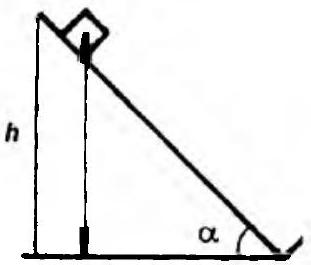
\includegraphics[max width=\textwidth, center]{2025_07_01_5b3ff9fa0d508c8e9f17g-037}

Fig. 1.14\\
A) 8 m ;\\
B) 9 m ;\\
C) $8,5 \mathrm{~m}$ ;\\
D) 6 m ;\\
E) 4 m ;\\
F) 10 m .\\
1.158. O minge de tenis de câmp cu masa de 50 g şi viteza de $180 \mathrm{~km} / \mathrm{h}$ loveşte terenul perfect elastic sub unghiul de $60^{\circ}$ față de verticală. Durata impactului este de $10^{-3} \mathrm{~s}$. Forța cu care mingea loveşte terenul este:\\
А) 1750 N ;\\
B) 2500 N ;\\
C) 3000 N ;\\
D) 1500 N ;\\
E) 2000 N ;\\
F) 4000 N .\\
(Constantin Neguțu)\\
1.159.* Să se afle masa Soarelui, cunoscând viteza liniară de rotație a Pământului în jurul Soarelui, $v=30 \mathrm{~km} / \mathrm{s}$, raza orbitei Pământului, presupusă circulară, $R=1,5 \cdot 10^{10} \mathrm{~km}$ şi constanta atracției universale, $k=6,67 \cdot 10^{-11} \mathrm{Nm}^{2} / \mathrm{kg}^{2}$.\\
A) $2 \cdot 10^{30} \mathrm{~kg}$;\\
B) $2 \cdot 10^{32} \mathrm{~kg}$ :\\
C) $2 \cdot 10^{27} \mathrm{~kg}$;\\
D) $1,2 \cdot 10^{30} \mathrm{~kg}$;\\
E) $2 \cdot 10^{34} \mathrm{~kg}$;\\
F) $2 \cdot 10^{24} \mathrm{~kg}$.\\
(Constantin Neguțu)\\
1.160. Variația energiei cinetice a unui corp asupra căruia acționează un sistem de forţe este egalã cu:\\
A) variația energiei potențiale; B) zero; C) lucrul mecanic efectuat de forța rezultantă ce acționează asupra corpului în timpul acestei variații; D) lucrul mecanic efectuat de câmpul gravitațional; E) momentul forței rezultante față de centrul de masă al corpului; F) impulsul forței rezultante.\\
(Constantin Neguțu)\\
1.161.* În cazul ciocnirii perfect plastice a două corpuri se conservă:\\
A) energia cinetică a sistemului B) energia potentială a sistemului; C) impulsul sistemului; D) energia cinetică şi impulsul sistemului; E) impulsul şi energia potentială a sistemului; F) energia potențială, energia cinetică şi impulsul sistemului.\\
(Constantin Neguțu)\\
1.162.* Un corp cade liber de la înălţimea de 100 m . După 4 s de cădere este ciocnit plastic de un corp cu aceeaşi masă, având viteza de $20 \mathrm{~m} / \mathrm{s}$ orientată orizontal. Distanța parcursă pe orizontală față de locul ciocnirii este ( $\mathrm{g}=10 \mathrm{~m} / \mathrm{s}^{2}$ ):\\
A) 82 m ;\\
B) $0,82 \mathrm{~m}$;\\
C) 0 ;\\
D) $18,2 \mathrm{~m}$;\\
E) $8,2 \mathrm{~m}$;\\
F) 10 m .\\
(Constantin Neguţu)\\
1.163.* Doi motociclişti aleargă cu o mişcare uniformă pe același cerc s.r.ind in același moment din acelaşi punct. Vitezele lor sunt $v_{1}=54 \mathrm{~km} / \mathrm{h}$ şi $:=43,2 \mathrm{~km} / \mathrm{h}$. Neglijând mişcarea accelerată de la pornire, numărul de rotații 2.5 : are unul îl prinde pe celălalt din urmă în punctul de plecare este:\\
.A) 1; B) 2;\\
C) 3 ;\\
D) 4;\\
E) 5 ; F) 6.\\
(Constantin Neguțu)\\
1.164.* De la o înălțime $h_{0}$ față de un plan orizontal se lasă liberă, fară挺 inițială, o bilă. Bila loveşte planul cu viteza $v_{0}$ şi se întoarce cu viteza $=\approx \gamma_{0}$ ( $v_{0}$ şi $v_{1}$ in valori absolute). Durata totală a mişcării bilei până ce - 2 :-51a se opreşte este:\\
A) $\sqrt{\frac{2 h_{0}}{g}} \frac{1+e}{1-e}$;\\
B) $\sqrt{\frac{2 h_{0}}{g}} \frac{e}{1-e}$;\\
C) $\frac{1}{2} \sqrt{\frac{2 h_{0}}{g}} \frac{e}{1-e}$;\\
D) $2 \sqrt{\frac{2 h_{0}}{g}} \frac{e}{1+e}$;\\
Е) $2 \sqrt{\frac{2 h_{0}}{g}} \frac{1+e}{1-e}$;\\
F) $\sqrt{\frac{2 h_{0}}{g}} \frac{e}{1+e}$.\\
(Constantin Neguțu)\\
1.165. Un tren de masă $m=1200 \mathrm{t}$ are o viteză inițială $v=72 \mathrm{~km} / \mathrm{h}$. - ésicientul de frecare dintre tren şi şine este $\mu=0,05$. Ce fortă de frânare trebuie ec. cată. pentru ca trenul să fie oprit în 20 s de la oprirea motorului electric al crotivei (se consideră $g=10 \mathrm{~m} / \mathrm{s}^{2}$ )?\\
A) $6 \cdot 10^{5} \mathrm{~N}$;\\
B) $3 \cdot 10^{6} \mathrm{~N}$;\\
C) $8 \cdot 10^{4} \mathrm{~N}$;\\
Di $5 \cdot 10^{5} \mathrm{~N}$;\\
E) $4,5 \cdot 10^{6} \mathrm{~N}$;\\
F) $8,3 \cdot 10^{5} \mathrm{~N}$.\\
(Cristian Toma)\\
1.166.* Un corp de masă $m=30 \mathrm{~kg}$ se deplasează cu viteza $v=30 \mathrm{~m} / \mathrm{s}$. Pe 2:-: corp este pus un corp de masă $m^{\prime}$, după acest impact corpurile deplasându-se $\therefore$...eza $v^{\prime}=10 \mathrm{~m} / \mathrm{s}$. Care este masa $m^{\prime}$ a celui de-al doilea corp?\\
A) 20 kg ;\\
B) 60 kg ;\\
C) 35 kg ;\\
D) 47 kg ;\\
E) 52 kg ;\\
F) 74 kg .\\
(Cristian Toma)\\
1.167. În ce condiţii vitezele relative $\vec{v}_{1}$ şi $\vec{v}_{2}$ ale celor două şenile ale unui - zur considerate în raport cu centrul tractorului sunt egale în modul satisfăcând - eria $\left|\vec{v}_{1}\right|=\left|\vec{v}_{2}\right|=|\vec{a}|$ (unde $\vec{a}$ este un vector cunoscut de modul nenul) astfel ca .erul tractorului să rămână în repaus?\\
A) $\vec{v}_{1}=\vec{a} ; \vec{v}_{2}=\vec{a}$;\\
B) $\left.\vec{v}_{1}=\vec{a} ; \vec{v}_{2}=\vec{a} / 2 ; \mathrm{C}\right) \vec{v}_{1}=-\vec{a} ; \vec{v}_{2}=\vec{a} ;$\\
D) $\left.\left.\vec{v}_{1}=-\vec{a} ; \vec{v}_{2}=-\vec{a} / 2 ; \mathrm{E}\right) \vec{v}_{1}=-\vec{a} ; \vec{v}_{2}=-\vec{a} ; \mathrm{F}\right) \bar{v}_{1}=-\vec{a} ; \vec{v}_{2}=\vec{a} / 2$.\\
(Cristian Toma)\\
1.168. Să se calculeze coeficientul de frecare $\mu$ dintre un automobil de 500 kg şi sol dacă pentru a se deplasa cu viteza de $108 \mathrm{~km} / \mathrm{h}$ aceasta foloseşte o putere de $3 \times 10^{4} \mathrm{~W}$ (se consideră $g=10 \mathrm{~m} / \mathrm{s}^{2}$ ).\\
A) $\mu=0,1$; B) $\mu=0,01$; C) $\mu=0,2$; D) $\mu=0,25$; E) $\mu=0,15$; F) $\mu=0,02$.\\
(Cristian Toma)\\
1.169. La o curbă de rază $R=49 \mathrm{~m}$ drumul a fost înclinat în raport cu suprafata orizontală la unghiul $\alpha=\operatorname{arctg} 0,1$. Considerând $g=10 \mathrm{~m} / \mathrm{s}^{2}$, să se afle pentru ce viteză a fost proiectat drumul respectiv.\\
A) $v=7 \mathrm{~m} / \mathrm{s}$;\\
B) $v=1 \mathrm{~m} / \mathrm{s}$;\\
C) $v=49 \mathrm{~m} / \mathrm{s}$;\\
D) $v=14 \mathrm{~m} / \mathrm{s}$;\\
E) $v=1,4 \mathrm{~m} / \mathrm{s} ; \mathrm{F}) v=4,9 \mathrm{~m} / \mathrm{s}$.\\
(Cristian Toma)\\
1.170.* Un ceasornic cu cadran este pornit la ora 12 (când orarul, minutarul şi secundarul sunt aliniate). La ce unghi cu axa ce uneşte centrul cadranului cu poziția corespunzătoare orei 12 se întâlnesc din nou, pentru prima oară, secundarul şi minutarul?\\
А) $\frac{\pi}{2} \mathrm{rad}$;\\
B) $\frac{\pi}{4} \mathrm{rad}$;\\
C) $\frac{\pi}{59} \mathrm{rad}$;\\
D) $\frac{\pi}{60} \mathrm{rad}$;\\
E) $\frac{2 \pi}{59} \mathrm{rad}$;\\
F) $\frac{2 \pi}{60} \mathrm{rad}$.\\
(Cristian Toma)\\
1.171.* Un corp lansat cu viteza $\nu=10 \mathrm{~m} / \mathrm{s}$ de la sol, sub unghiul $\alpha$ față de orizontală, revine la sol la distanța de $5 \sqrt{3} \mathrm{~m}$ față de poziția de plecare. Sã se afle unghiul $\alpha$ (se consideră $g=10 \mathrm{~m} / \mathrm{s}^{2}$ ).\\
A) $\frac{\pi}{2}$;\\
в) $\frac{\pi}{4}$;\\
C) $\frac{\pi}{3}$;\\
b) $\frac{\pi}{6}$;\\
E) $\frac{\pi}{8}$;\\
F) $\frac{\pi \sqrt{3}}{2}$.\\
(Cristian Toma)\\
1.172.* Un corp de masă $m$ este aruncat de la sol din punctul O cu viteza inițialà $\nu$ sub un unghi $\alpha$ în raport cu o axă $O x$ conținută în planul solului, astfel încât proiecția poziției sale pe sol să aparțină permanent acestei axe Ox . Acest corp\\
--: la sol în punctul M. Să se afle valoarea unghiului $\alpha$ astfel încât distanța : 4 : in modul) să fie maximă.\\
A) $\alpha \in\left\{\frac{\pi}{4}\right\} ;$\\
в) $\alpha \in\left\{\frac{\pi}{2}, \pi\right\}$;\\
C) $\alpha \in\left\{\frac{\pi}{4}, \frac{3 \pi}{4}\right\}$;\\
D) $\alpha \in\left\{\frac{\pi}{4},-\frac{\pi}{4}\right\}$;\\
E) $\alpha \in\left\{\frac{3 \pi}{4}\right\}$;\\
F) $\alpha \in\left\{-\frac{\pi}{4}\right\}$.\\
(Cristian Toma)\\
1.173. Metroul parcurge distanța dintre două stații consecutive în 2 min 20 s , radregand o mişcare uniform accelerată urmată de una uniformă și apoi de una ๓. żrm încetinită. Dacă accelerațiile inițială și finală sunt egale în valoare нг. .ută, $|a|=1 \mathrm{~m} / \mathrm{s}^{2}$, şi viteza maximă la care ajunge trenul este $v_{m}=90 \mathrm{~km} / \mathrm{h}$ să < 二etermine distanța dintre cele două stații.\\
.A) $2,5 \mathrm{~km}$;\\
B) 2225 m ;\\
C) 2875 m ;\\
D) $1,25 \mathrm{~km}$;\\
E) 12500 m ;\\
F) $22,5 \mathrm{~km}$.\\
(Ion Gurgu)\\
1.174. Un corp este aruncat pe verticală în sus cu viteza inițială $v_{0}=10 \mathrm{~m} / \mathrm{s}$. ${ }^{2}$...e cât timp acesta se va găsi la înălțimea $h=10 \mathrm{~m}$ ?\\
A) 1 s ; B) imposibil; C) 10 s ; D) $1,5 \mathrm{~s}$; E) 1 h ; F) $0,5 \mathrm{~s}$.\\
(Ion Gurgu)\\
1.175. Un glonte cu masa $m=25 \mathrm{~g}$ pătrunde într-o scândură pe distanța $=5 \mathrm{~cm}$. Dacă viteza inițială a glontelui este $v_{0}=500 \mathrm{~m} / \mathrm{s}$, ce impuls ar primi o cỉาdură identică, de grosime 2 cm .\\
A) 2 kg ;\\
B) $2,8 \mathrm{Ns}$;\\
C) $5,6 \mathrm{Ns}$;\\
D) nu primeşte impuls;\\
E) $1,4 \mathrm{Nm}$; F) $1,4 \mathrm{Ns}$.\\
(Ion Gurgu)\\
1.176. De capetele unui fir trecut peste un scripete sunt legate două corpuri cu - zesele $m_{1}=10 \mathrm{~g}$ şi $m_{2}=50 \mathrm{~g}$. Dacă sistemul este lăsat liber, să se calculeze -islțimea maximă la care se ridică masa $m_{1}$, cunoscând $h_{2}=50 \mathrm{~cm}$ (Fig. 1.15). Se ::nsideră $g=10 \mathrm{~m} / \mathrm{s}^{2}$.\\
А) $5 / 6 \mathrm{~m}$;\\
B) $6 / 5 \mathrm{~m}$;\\
C) 1 m ;\\
D) nu se ridică;\\
E) $0,5 \mathrm{~m}$;\\
F) $1,5 \mathrm{~m}$.\\
1.177. Un corp este aruncat cu viteza inițială $v_{0}=6 \mathrm{~m} / \mathrm{s}$, pe un plan înclinat de unghi $\alpha=45^{\circ}$. ştiind că mişcarea se face cu frecare şi timpul de coborâre este de 3 ori mai mare decât la urcare, să se determine înălțimea până la care a urcat corpul.\\
A) 1 m ;\\
B) $1,1 \mathrm{~m}$;\\
C) $0,9 \mathrm{~m}$;\\
D) imposibil;\\
E) $1,5 \mathrm{~m}$;\\
F) $0,1 \mathrm{~m}$.\\
(Ion Gurgu)\\
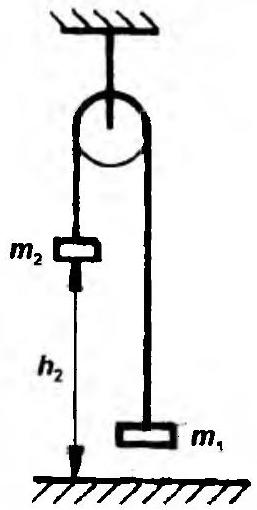
\includegraphics[max width=\textwidth, center]{2025_07_01_5b3ff9fa0d508c8e9f17g-042}

Fig. 1.15\\
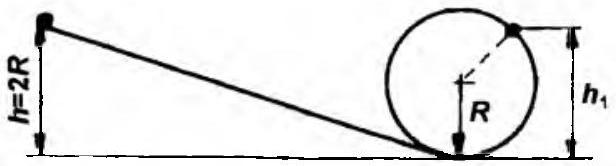
\includegraphics[max width=\textwidth, center]{2025_07_01_5b3ff9fa0d508c8e9f17g-042(1)}

Fig. 1.16\\
1.178.* Un corp coboară liber, fără frecare, pe un plan înclinat şi de la baza acestuia îşi continuă mişcarea pe o traiectorie circulară de rază $R=1 \mathrm{~m}$ (Fig. 1.16). Dacă corpul coboară de la înălțimea $h=2 R$, să se determine înălțimea $h_{1}$ la care ajunge corpul pe traiectoria circulară.\\
A) $1,0 \mathrm{~m}$; B) $0,1 \mathrm{~m}$; C) imposibil; D) $1,61 \mathrm{~m}$; E) $2,0 \mathrm{~m}$; F) $0,5 \mathrm{~m}$.\\
(Ion Gurgu)\\
1.179. Din vârful unui turn cu înălțimea $h=60 \mathrm{~m}$ este aruncat în sus un corp cu viteza inițială $v_{0}=20 \mathrm{~m} / \mathrm{s}$. Cu ce viteză va atinge corpul solul ? $\left(g=10 \mathrm{~m} / \mathrm{s}^{2}\right)$\\
A) $30 \mathrm{~m} / \mathrm{s}$; B) $60 \mathrm{~m} / \mathrm{s}$; C) $40 \mathrm{~m} / \mathrm{s}$; D) $120 \mathrm{~m} / \mathrm{s}$; E) $20 \mathrm{~m} / \mathrm{s}$; F) $80 \mathrm{~m} / \mathrm{s}$.\\
(Marcel Dobre)\\
1.180. Un corp este aruncat fără frecare pe un plan înclinat. La 1s, respectiv 2 s , din momentul aruncării corpul se află la distantá de $0,3 \mathrm{~m}$ de punctul de aruncare. Să se calculeze viteza inițială a corpului.\\
A) $4,5 \mathrm{~m} / \mathrm{s}$;\\
B) $45 \mathrm{~m} / \mathrm{s}$;\\
C) $0,45 \mathrm{~m} / \mathrm{s}$;\\
D) $0,9 \mathrm{~m} / \mathrm{s}$;\\
E) $1,5 \mathrm{~m} / \mathrm{s}$;\\
F) $2 \mathrm{~m} / \mathrm{s}$.

1.181.*$O$ piatră este aruncată cu $v_{0}=20 \mathrm{~m} / \mathrm{s}$ sub unghi $\alpha=60^{\circ}$ cu ranntala.Să se calculeze raza de curbură în punctul situat la înălțimea maximă. $-=10 \mathrm{~m} / \mathrm{s}^{2}$ )\\
A) 1 m ;\\
B) 10 m ;\\
C) 40 m ;\\
D) 18 m ;\\
E) 20 m ;\\
F) 5 m .\\
(Marcel Dobre)

1.182.O porţiune de şosea prezintă o pantă de 0,05 .Pe această şosea un运-mobil cu masa $m=150 \mathrm{~kg}$ coboară uniform având motorul decuplat,cu viteza $x: 0 \mathrm{~m} / \mathrm{s}$ .Care trebuie să fie puterea motorului pentru ca automobilul să urce น.¿rm aceeaşi pantã cu aceeaşi viteză ?$\left(g=10 \mathrm{~m} / \mathrm{s}^{2}\right)$\\
A) 15000 W ;\\
B) 1500 W ;\\
C) 3500 W ;\\
D) 12000 W ;\\
E) 25000 W ;\\
F) 10000 W .\\
(Marcel Dobre)

1.183.*O piatră cu masa $m=0,2 \mathrm{~kg}$ este aruncată oblic pe o suprafață rzontală şi revine pe aceeaşi suprafață la o distanță $S=5 \mathrm{~m}$ de locul aruncării диса̀ $t=1 \mathrm{~s}$ .Dacă se neglijează frecarea,să se afle lucrul mecanic necesar pentru $\therefore$ ごtuarea aruncării.$\left(g=10 \mathrm{~m} / \mathrm{s}^{2}\right)$\\
A) 10 J ;\\
B) 15 J ;\\
C) 25 J ;\\
D) 100 J ;\\
E) 60 J ;\\
F) 5 J .\\
(Marcel Dobre)\\
1.184.*Sub acțiunea unui impuls inițial o greutate legată cu un fir de tavan zerie un cerc situat în plan orizontal la o distanță de $1,5 \mathrm{~m}$ de tavan.Care este こここența rotațiilor greutății ?$\left(g=10 \mathrm{~m} / \mathrm{s}^{2}\right)$\\
A) $0,91 \mathrm{~s}^{-1}$ ;\\
B) $0,41 \mathrm{~s}^{-1}$ ;\\
C) $0,5 \mathrm{~s}^{-1}$ ;\\
D) $1,14 \mathrm{~s}^{-1}$ ;\\
E) $2,4 \mathrm{~s}^{-1}$ ;\\
F) $3,2 \mathrm{~s}^{-1}$ .\\
(Marcel Dobre)\\
1.185.Sub acțiunea unei forțe $F_{1}=9 \mathrm{~N}$ ,un punct material se mişcă cu m:=lerația $a_{1}=3 \mathrm{~m} / \mathrm{s}^{2}$ .Cu ce accelerație se va mişca acesta sub acțiunea unei tre $F_{2}=6 \mathrm{~N}$ ?\\
A) $1 \mathrm{~m} / \mathrm{s}^{2}$ ;\\
B) $2 \mathrm{~m} / \mathrm{s}^{2}$ ;\\
C) $5 \mathrm{~m} / \mathrm{s}^{2}$ ;\\
D) $2,5 \mathrm{~m} / \mathrm{s}^{2}$ ;\\
E)$-3 \mathrm{~m} / \mathrm{s}^{2}$ ;F)$-5 \mathrm{~m} / \mathrm{s}^{2}$ .\\
1.186. O minge cu masa $m=0,2 \mathrm{~kg}$ a căpătat, după lovire, o viteză $v=15 \mathrm{~m} / \mathrm{s}$. Dacă durata lovirii a fost $\Delta t=10^{-2} \mathrm{~s}$, să se afle forta medie de lovire.\\
A) 300 N ;\\
B) 1 kN ;\\
C) 500 N ;\\
D) $0,2 \mathrm{kN}$;\\
E) $125,5 \mathrm{~N}$;\\
F) 15 kN .\\
(Marin Cilea)\\
1.187. Un camion cu masa $m=10 \mathrm{t}$ porneşte cu accelerația $a=0,55 \mathrm{~m} / \mathrm{s}^{2}$. ${ }^{\text {a }}$ tiind că forțele de frecare (de rezistență) au valoarea de 500 N , să se afle forța de tractiune a motorului.\\
A) 2 kN ;\\
B) $2,5 \mathrm{kN}$;\\
C) 10 kN ;\\
(D) 6 kN ;\\
E) $10^{3} \mathrm{~N}$; F) 500 N .\\
(Marin Cilea)\\
1.188. O săniuță coboară liber un deal de lungime $l=50 \mathrm{~m}$ intr-un timp $t=10 \mathrm{~s}$. Cu ce viteză a ajuns ea la baza dealului ?\\
A) $3 \mathrm{~m} / \mathrm{s}$;\\
B) $1 \mathrm{~m} / \mathrm{s}$;\\
C) $4,5 \mathrm{~m} / \mathrm{s}$;\\
D) $50 \mathrm{~m} / \mathrm{s}$;\\
E) $25 \mathrm{~m} / \mathrm{s}$;\\
F) $10 \mathrm{~m} / \mathrm{s}$.\\
(Marin Cilea)\\
1.189. Un corp aruncat vertical în sus a revenit pe pământ după $\tau=10 \mathrm{~s}$. Cu ce viteză initială a fost aruncat corpul ? ( $g=10 \mathrm{~m} / \mathrm{s}^{2}$ )\\
A) $10 \mathrm{~m} / \mathrm{s}$;\\
B) $20 \mathrm{~m} / \mathrm{s}$;\\
C) $50 \mathrm{~m} / \mathrm{s}$;\\
D) $25 \mathrm{~m} / \mathrm{s}$;\\
E) $100 \mathrm{~m} / \mathrm{s}$;\\
F) $15 \mathrm{~m} / \mathrm{s}$.\\
(Marin Cilea)\\
1.190.* Un autoturism cu masa $m=1$ t merge cu viteza $v=10 \mathrm{~m} / \mathrm{s}$ peste un pod convex, cu raza de curbură $R=100 \mathrm{~m}$. Ce apăsare exercită autoturismul asupra podului în punctul superior? ( $g=10 \mathrm{~m} / \mathrm{s}^{2}$ )\\
A) 1 kN ;\\
B) $10^{4} \mathrm{~N}$;\\
C) $280,6 \mathrm{~N}$;\\
D) 0 N ;\\
E) 9 kN ; F) 500 N .\\
(Marin Cilea)\\
1.191. Un resort a fost comprimat cu $x=4 \mathrm{~cm}$ sub acțiunea unei forțe $F=25 \mathrm{~N}$. Calculați energia potentială a resortului.\\
A) 10 J ;\\
B) 5 J ;\\
C) 1 J ;\\
D) $0,5 \mathrm{~J}$;\\
E) 25 J ; F) 8 J .\\
(Marin Cilea)\\
1.192.* Un corp cu masa $m_{1}=0,5 \mathrm{~kg}$ şi viteza $v_{1}=10 \mathrm{~m} / \mathrm{s}$ loveşte un alt corp care se mişcă spre el pe aceeaşi direcție. După ciocnire corpurile se opresc. Calculați modulul impulsului pentru cel de-al doilea corp.\\
A) $10 \mathrm{~kg} \cdot \frac{\mathrm{~m}}{\mathrm{~s}}$ ;\\
B) $3 \mathrm{~N} \cdot \mathrm{~s}$ ;\\
C) $5 \mathrm{~N} \cdot \mathrm{~s}$ ;\\
D) $4 \frac{\mathrm{~kg} \cdot \mathrm{~m}}{\mathrm{~s}}$ ;\\
Е) $0,5 \mathrm{~N} \cdot \mathrm{~s}$ ;\\
F) $12,3 \mathrm{~N} \cdot \mathrm{~m}$ .\\
(Marin Cilea)\\
1.193.Impulsul unui corp este $p=10 \mathrm{~N} \cdot \mathrm{~s}$ ,iar energia cinetică $E_{c}=10 \mathrm{~J}$ .Să -: 2 masa corpului.\\
A) $1 \mathrm{~kg} ; \mathrm{B}) 3 \mathrm{~kg}$ ;\\
C) 5 kg ;\\
D) 7 kg ;\\
E) 9 kg ;\\
F) 11 kg .\\
(Marin Cilea)

1.194.Un corp cu masa $m=1 \mathrm{~kg}$ ,fără viteză inițială,coboară fără frecare pe m zlan înclinat de înălțime $h=5 \mathrm{~m}$ .Ajungând la baza planului,corpul se neasează cu frecare pe o suprafață plană orizontală până se opreşte.Să se ユどaleze timpul total de mişcare pe planul înclinat şi pe cel orizontal.Se dau: $:=30^{\circ}, \mu=0,2, g=10 \mathrm{~m} / \mathrm{s}^{2}$.\\
A) 7 s ;\\
B) 14 s ;\\
C) 2 s ;\\
D) 5 s ;\\
E) 6 s ;\\
F) $4,2 \mathrm{~s}$ .\\
(Tatiana Pop)\\
1.195.Un punct material este lansat în sus de-a lungul unui plan înclinat care r.r.ează unghiul $\alpha=45^{\circ}$ cu orizontala,cu viteza inițială $v_{0}=6 \mathrm{~m} / \mathrm{s}$ .Mişcarea se $\mathrm{h}_{\mathrm{i}}=\mathrm{cu}$ frecare,coeficientul de frecare la alunecare între corp şi planul înclinat Face $\mu=0,2$ .Dacă din punctul de înălțime maximă,corpul coboară cu viteza mală nulă,de câte ori este mai mare timpul de coborâre până la baza planului, de timpul de urcare?Se dă $g=10 \mathrm{~m} / \mathrm{s}^{2}$ .\\
A) 1,22 ;\\
B) 1,4 ;\\
C) 2 ;\\
D) 5 ;\\
E) 6 ;F) 2,32 .\\
(Tatiana Pop)\\
1.196.Un corp cade liber de la o înălțime de 490 m .Ce spațiu străbate el în $u=$ na secundă a mişcării ?$\left(g=9,80 \mathrm{~m} / \mathrm{s}^{2}\right)$\\
A) 98 m ;\\
B) $93,1 \mathrm{~m}$ ;\\
C) $9,8 \mathrm{~m}$ ;\\
D) 108 m ;\\
E) 100 m ;\\
F) 88,6 .\\
(Tatiana Pop)\\
1.197.Un automobil cu masa 1000 kg porneşte din repaus şi ajunge la viteza $\nsimeq 30 \mathrm{~m} / \mathrm{s}$ după ce parcurge 500 m pe un drum orizontal.Să se calculeze forţa de restiune a motorului,dacă forța de frecare este de 200 N .\\
A)$F=1000 \mathrm{~N}$ ;\\
В)$F=1050 \mathrm{~N}$ ;\\
C)$F=1100 \mathrm{~N}$ ;\\
D)$F=900 \mathrm{~N}$ ;\\
E)$F=1150 \mathrm{~N}$ ;\\
F) 1350 N .\\
1.198.* Un corp se mişcă uniform pe un cerc de rază $R=10 \mathrm{~m}$, sub acțiunea unei forțe centripete $F=100 \mathrm{~N}$. Lucrul mecanic efectuat de această forță într-o perioadă a mişcării este:\\
A) $L=2000 \pi \mathrm{~J}$;\\
B) $L=1000 \pi \mathrm{~J}$;\\
C) $L=0 \mathrm{~J}$;\\
D) $L=3000 \pi \mathrm{~J}$;\\
E) $L=1000 \mathrm{~J}$;\\
F) $L=100 \pi \mathrm{~J}$.\\
(Tatiana Pop)\\
1.199. Firul $A B$ inextensibil și de masă neglijabilă, fixat în $A$, are prins în $B$ un corp cu masa de 2 kg . Se scoate firul din poziția de echilibru, astfel încât formează cu verticala unghiul de $60^{\circ}$. Se lasă corpul liber. Tensiunea din fir, când acesta face cu verticala unghiul de $30^{\circ}\left(g=10 \mathrm{~m} / \mathrm{s}^{2}\right)$, este:\\
A) $F=1,7 \mathrm{~N}$;\\
B) $F=73,1 \mathrm{~N}$;\\
C) $F=20 \mathrm{~N}$;\\
D) $F=31,9 \mathrm{~N}$;\\
E) $F=40 \mathrm{~N}$;\\
F) $24,5 \mathrm{~N}$.\\
(Tatiana Pop)\\
1.200. Pentru a deplasa un corp în sus pe un plan înclinat cu unghiul de $45^{\circ}$ este necesară o forță tangențială minimă de 30 N , iar pentru a-l menține în repaus, forța tangentială minimă este de 15 N , îndreptată în acelaşi sens ca şi prima. Care este coeficientul de frecare dintre corp şi planul inclinat ?\\
А) 0,5 ;\\
B) 0,1 ;\\
C) $3 / 4$;\\
D) $1 / 3$;\\
E) 0,6 ;\\
F) 0,24 .\\
(Tatiana Pop)\\
1.201.* Un corp execută o mişcare oscilatorie armonică. Pentru a îndepărta corpul din poziția de repaus până la elongația maximă se cheltuieşte un lucru mecanic $L=0,5 \mathrm{~J}$. Fortă elastică care acționează asupra corpului în acest punct este $F=2,5 \mathrm{~N}$. Care este amplitudinea mişcării oscilatorii?\\
A) $0,25 \mathrm{~m}$;\\
B) $0,3 \mathrm{~m}$;\\
C) $0,35 \mathrm{~m}$;\\
D) $0,4 \mathrm{~m}$;\\
E) $0,5 \mathrm{~m}$;\\
F) $0,55 \mathrm{~m}$.\\
(Tatiana Pop)\\
1.202. Ecuația mişcării unui mobil este $x=2+6 t-t^{2}$ (valorile exprimate în Sistemul Internațional). După ce timp viteza mobilului este egală cu o treime din viteza inițială ?\\
A) $1 / 3 \mathrm{~s}$;\\
B) 4 s ;\\
C) 1 s ;\\
D) $0,5 \mathrm{~s}$;\\
E) 2 s ;\\
F) 3 s .\\
(Mona Mihăilescu)\\
1.203. Un corp parcurge în mişcare uniform accelerată cu viteza inițială $v_{0}, o$ distantă $s=96 \mathrm{~m}$. Prima jumătate o parcurge în $t_{1}=8 \mathrm{~s}$, iar cealaltă jumătate în $t_{2}=4 \mathrm{~s}$. Se cere accelerația corpului.\\
A) $3,2 \mathrm{~m} / \mathrm{s}^{2}$ ;\\
B) $1,4 \mathrm{~m} / \mathrm{s}^{2}$ ;\\
C) $2,4 \mathrm{~m} / \mathrm{s}^{2}$ ;\\
D) $5 \mathrm{~m} / \mathrm{s}^{2}$ ;\\
E) $6 \mathrm{~m} / \mathrm{s}^{2}$ ;\\
F) $1 \mathrm{~m} / \mathrm{s}^{2}$ .\\
(Mona Mihǎilescu)\\
1.204.Un corp de masă $m=4 \mathrm{~kg}$ este acționat cu o forță $F=60 \mathrm{~N}$ orientată x :erticală în sus.Cu ce accelerație se mişcă corpul ?Se neglijează frecarea.Se立 $\xi=10 \mathrm{~m} / \mathrm{s}^{2}$ .\\
A) $25 \mathrm{~m} / \mathrm{s}^{2}$ sus;B) $5 \mathrm{~m} / \mathrm{s}^{2}$ jos;\\
C) $400 \mathrm{~m} / \mathrm{s}^{2}$ sus;\\
D) $25 \mathrm{~m} / \mathrm{s}^{2}$ jos;\\
E) $5 \mathrm{~m} / \mathrm{s}^{2}$ sus;\\
F) $20 \mathrm{~m} / \mathrm{s}^{2} \mathrm{jos}$ .\\
(Mona Mihăilescu)\\
1.205.Un resort aflat pe un plan orizontal este fixat la un capăt,iar la celălalt :¿ミat un corp de masă $m$ .La momentul inițial resortul e netensionat,se imprimă Trélui $m$ viteza $v_{0}$ în sensul destinderii resortului.Dacă se cunoaşte constanta こescică $K$ ,se cere deformația maximă în lipsa frecărilor.\\
л)$\frac{m v_{0}}{K}$ ;\\
В)$\frac{\sqrt{m v_{0}}}{K}$ ;\\
C)$v_{0} \sqrt{\frac{m}{K}}$ ;\\
D)$v_{0} \sqrt{\frac{K}{m}}$ ;\\
E)$\frac{v_{0}}{m} \sqrt{K}$ ;\\
F)$v_{0} \sqrt{\frac{2 m}{K}}$ .\\
(Mona Mihăilescu)\\
1.206.*Acele unui ceasornic au lungimile $l_{1}=3 \mathrm{~cm}$(orarul)şi $l_{2}=4,5 \mathrm{~cm}$ T.tarul).Care este raportul vitezelor periferice $v_{1} / v_{2}$ ale celor două ace me-atoare?\\
A) $2 / 3$ ;\\
B)8;\\
C) $1 / 3$ ;\\
D)1/18;\\
E) $1 / 90 ; 2 / 30$ .\\
(Mona Mihăilescu)\\
1.207.Un corp cu greutatea de 10 N cade liber un sfert de minut.Care este -ạria impulsului corpului neglijând frecările( $g=10 \mathrm{~m} / \mathrm{s}^{2}$ ).\\
A) $250 \mathrm{kgm} / \mathrm{s}$ ;\\
B) $15 \mathrm{kgm} / \mathrm{s}$ ;\\
C) $150 \mathrm{kgm} / \mathrm{s}$ ;\\
D) $1500 \mathrm{kgm} / \mathrm{s}$ ;\\
E) $25 \mathrm{kgm} / \mathrm{s}$ ;\\
F) $2,5 \mathrm{kgm} / \mathrm{s}$ .\\
(Mona Mihăilescu)\\
1.208.Un corp cade în câmpul gravitațional al unui astru,fără atmosferă,cu 2:-ierația gravitațională $g_{a}=2 \mathrm{~m} / \mathrm{s}^{2}$ .Să se determine de la ce înălțime trebuie să Entru a parcurge spațiul $h=3 \mathrm{~m}$ în timpul ultimei secunde a căderii sale.\\
A) 16 m ;\\
B) $2,85 \mathrm{~m}$ ;\\
C) 3 m ;\\
D) 4 m ;\\
E) $6,15 \mathrm{~m}$ ;\\
F) 8 m .\\
1.209. Un cilindru gol se mişcă pe un plan orizontal cu o accelerație $a=g$. Pe partea interioară a cilindrului se poate mişca fără frecare o mică sferă cu masa $m$. Care este unghiul pe care îl face raza vectoare a poziției de echilibru al sferei cu verticala ?\\
A) $90^{\circ}$;\\
B) $45^{\circ}$;\\
C) $30^{\circ}$;\\
D) $60^{\circ}$;\\
E) $180^{\circ}$;\\
F) $0^{\circ}$.\\
(Alexandru M. Preda)\\
1.210. Pe un plan orizontal se află o scândură cu masa $m=1 \mathrm{~kg}$, iar pe scândura un corp mic cu greutatea $G_{1}=20 \mathrm{~N}$ (Fig. 1.17). Ce forță orizontalã minimă, $F$, trebuie aplicată scândurii pentru ca ea să alunece de sub corp ? Se consideră coeficientul de frecare dintre corp şi scândură $\mu_{1}=0,25$, iar cel dintre scândură şi plan $\mu_{2}=0,50\left(g=10 \mathrm{~m} / \mathrm{s}^{2}\right)$.\\
A) 20 N ; B) 30 N ; C) $22,5 \mathrm{~N}$; D) 10 N ; E) $40,5 \mathrm{~N}$; F) $32,5 \mathrm{~N}$.\\
(Alexandru M. Preda)\\
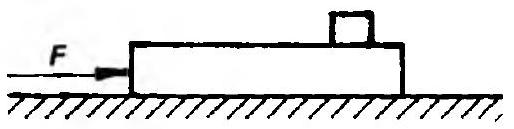
\includegraphics[max width=\textwidth, center]{2025_07_01_5b3ff9fa0d508c8e9f17g-048}

Fig. 1.17\\
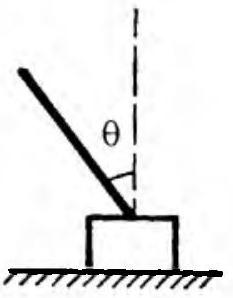
\includegraphics[max width=\textwidth, center]{2025_07_01_5b3ff9fa0d508c8e9f17g-048(1)}

Fig. 1.18\\
1.211. O cărămidă cu masa $m=5 \mathrm{~kg}$ se află pe un plan orizontal. Aceasta este deplasată uniform pe plan cu ajutorul unei cozi de lemn care face un unghi $\theta=30^{\circ}$ cu directia verticală (Fig. 1.18). Masa cozii este neglijabilă, iar coeficientul de frecare dintre cărămidă şi plan este $\mu=0,1$. Să se afle mărimea fortei, orientată de-a lungul cozii, necesară pentru a face cărămida să alunece cu viteză constantă pe plan ( $g=10 \mathrm{~m} / \mathrm{s}^{2}$ ).\\
A) 50 N ; B) 25 N ; C) $5,12 \mathrm{~N}$;(D) $12,09 \mathrm{~N}$; E) 5 N ; F) $20,5 \mathrm{~N}$.\\
(Alexandru M. Preda)\\
1.212. O cărămidă cu masa $m=5 \mathrm{~kg}$ este aşezată pe un perete vertical şi apăsată cu o forță, $F$, de jos in sus, care face cu orizontala un unghi $\theta=45^{\circ}$. Dacă se consideră coeficientul de frecare $\mu=0,3$ şi $g=10 \mathrm{~m} / \mathrm{s}^{2}$ să se calculeze mărimea minimă a forței $F$ necesară pentru ca să nu cadă cărămida în jos.

$$
\therefore \text { 三 (; B) } 35 \mathrm{~N} \text {; C) } 150,5 \mathrm{~N} \text {; D) } 200,25 \mathrm{~N} \text {; E) } 54,39 \mathrm{~N} \text {; F) } 5,25 \mathrm{~N} \text {. }
$$

(Alexandru M.Preda)\\
1.213.*Presupunem că Pământul este perfect sferic şi are raza $R=6400 \mathrm{~km}$ . こа::nsiderăm $g=10 \mathrm{~m} / \mathrm{s}^{2}$ în toate punctele de pe Pământ,să se afle cu cât se m.c⿱⿱一𫝀口八土azá greutatea unui om cu masa $m=100 \mathrm{~kg}$ când se deplasează de la pol la二五只\\
$\therefore 0 \mathrm{~N} ; \mathrm{B}) 3,37 \mathrm{~N}$ ;\\
C) $10,51 \mathrm{~N}$ ;\\
D) 50 N ;\\
E) $1,21 \mathrm{~N}$ ;F) $80,53 \mathrm{~N}$ .\\
(Alexandru M.Preda)\\
1.214.Un corp se deplasează în sensul pozitiv al axei $O x$ sub actiunea unei use $F(x)=7 x+3$ ,unde $F$ se exprimă în newtoni şi poziția $x$ în metri.Sub --ea acestei forţe corpul se deplasează între punctele $x_{1}=3 \mathrm{~m}$ şi $x_{2}=5 \mathrm{~m}$ . -ジ-1 mecanic efectuat de această forță are valoarea:\\
A) 124 J;B) 38 J;\\
C) 62 J ;\\
D) 31 J ;\\
E) 20 J ;\\
F) 50 J .\\
(Alexandru M.Preda)\\
1.215.Un avion având viteza de zbor(față de aerul înconjurător)de $234 \mathrm{~km} / \mathrm{h}$ स्व-:e să se deplaseze spre nord,în condițiile în care vântul bate spre est cu viteza $x:=5 \mathrm{~m} / \mathrm{s}$ .Se cere viteza de deplasare a avionului faţă de pământ,precum şi ữalul pe care trebuie să îl facă direcția de zbor a fuzelajului avionului cu direcția\\
A) $216 \mathrm{~km} / \mathrm{h}$ ; $\operatorname{arctg} \frac{5}{12}$ spre V-NV;\\
B) $216 \mathrm{~km} / \mathrm{h}$ ; $\operatorname{arctg} \frac{5}{12}$ spre E-NE;\\
C) $60 \mathrm{~m} / \mathrm{s}$ ; $\arcsin 0,416 \mathrm{spre} \mathrm{E}-\mathrm{NE}$ ;\\
D) $65 \mathrm{~m} / \mathrm{s}$ ; $\arcsin 0,75 \mathrm{spre} \mathrm{V}-\mathrm{NV}$ ;\\
E) $162,5 \mathrm{~km} / \mathrm{h}$ ; $\arcsin \frac{5}{13}$ spre V-NV;\\
F) $180 \mathrm{~km} / \mathrm{h} \arccos \frac{12}{13}$ spre E-NE.\\
(Corneliu Călin)\\
1.216.Un plan înclinat are rolul de a ridica greutați la înălțimea $h=4,4 \mathrm{~m}$ , -zhiul de înclinare fiind de $45^{\circ}$ .De la baza acestui plan se lansează în sus pe ...an cu viteza inițială $v_{0}=11 \mathrm{~m} / \mathrm{s}$ un corp ce se mişcă cu frecare,coeficientul de -ze are dintre corp şi plan fiind $\mu=0,1$ .Se cere timpul după care corpul ajunge la :apätul superior al planului înclinat.Se consideră $g=10 \mathrm{~m} / \mathrm{s}^{2}$ .\\
А) $0,78 \mathrm{~s}$ ;\\
B) 2 s ;\\
C) $1,41 \mathrm{~s}$ ;\\
D) $1,73 \mathrm{~s}$ ;\\
E) $0,707 \mathrm{~s}$ ;\\
F) $0,577 \mathrm{~s}$ .\\
1.217.* Se consideră sistemul de corpuri reprezentat în Fig. 1.19. Corpul de masă $m_{1}$ se află situat la o distanță mai mare decât $h$ față de scripete. În momentul când $m_{2}$ atinge solul, viteza corpurilor va fi:\\

A) $v=\sqrt{2 g h}$;\\
B) $v=\sqrt{\frac{2 m_{1} g h}{m_{1}+m_{2}}}$;\\
C) $v=\sqrt{\frac{\left(m_{1}+m_{2}\right) g h}{m_{1}}}$;\\
D) $v=\sqrt{\frac{m_{2}}{m_{1}} g h}$;\\
E) $v=\sqrt{\frac{2 m_{2} g h}{m_{1}+m_{2}}}$;\\
F) $v=\sqrt{g h}$.\\
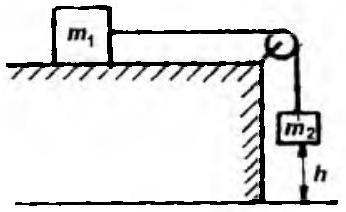
\includegraphics[max width=\textwidth, center]{2025_07_01_5b3ff9fa0d508c8e9f17g-050} Fig. 1.19\\

(Gheorghe Stanciu)\\
1.218. Sub acțiunea unui corp de masă $m^{\prime}$ un resort elastic suferă alungirea $\Delta l$. Suspendând resortul de tavanul unui mobil care suferă o mişcare pe un cerc de rază $R$, cu viteza $v$, să se arate dacă alungirea resortului este:\\
A) $\Delta l^{\prime}=\Delta l$;\\
В) $\Delta l^{\prime}=\Delta l \sqrt{\frac{v^{2}}{R}+g}$;\\
C) $\Delta l^{\prime}=\frac{\Delta l}{g} \sqrt{\frac{v^{4}}{R^{2}}+g^{2}}$;\\
D) $\Delta l^{\prime}=\frac{\Delta l}{g} \sqrt{\frac{v^{2}}{R^{4}}+g^{2}}$;\\
E) $\Delta l^{\prime}=\frac{\Delta l}{g} \sqrt{\frac{v^{2}}{R^{4}}-g^{2}}$;\\
F) $\Delta l^{\prime}=\Delta l \sqrt{v^{2}-g^{2}}$.\\
(Gheorghe Stanciu)\\
1.219. Un corp prismatic de masă $M$ se poate deplasa pe o suprafață orizontală fără frecare. Pe suprafața acestuia se află un corp de masă $m$, coeficientul de frecare dintre corpuri fiind $\mu$. Dacă asupra corpului $M$ acționează o forță $F$, astfel încât corpul de masă $m$ începe să alunece, accelerația acestuia fată de $M$ va fi :\\
A) $a=\mu \mathrm{mg}$;\\
B) $a=\frac{\mu M g}{m}$;\\
C) $a=\frac{\mu(M+m) g}{m}$;\\
D) $a=\frac{F-\mu m g}{M}-\mu g$;\\
(e) $a=\frac{F-\mu M g}{m}-\mu g$;\\
F) $a=\frac{F-\mu m g}{M+m}$.\\
(Gheorghe Stanciu)\\
1.220. Un plan înclinat sub unghiul $\alpha$, se poate deplasa fară frecare pe suprafâa orizontală. Un corp de masă $m$ se află pe plan. Sub acțiunea unei forțe planul începe să se deplaseze accelerat, cu accelerația $\vec{a}$, în direcția opusă mişcării corpului pe plan. Cunoscând coeficientul de frecare $\mu$ să se arate dacă accelerația corpului faţă de suprafața planului înclinat este:\\
A) $g \sin \alpha$;\\
B) $g \sin \alpha-a \cos \alpha$;\\
C) $g \sin \alpha-\mu \cos \alpha$;

$$
\begin{aligned}
& \text { D. } g \sin \alpha+a \cos \alpha-\mu(g \cos \alpha-a \sin \alpha) \text {; } \\
& \text { E. } g \sin \alpha-\mu(g \cos \alpha-a \sin \alpha) ; \quad \text { F) } \mu g \cos \alpha-(g \sin \alpha+a \cos \alpha) \text {. }
\end{aligned}
$$

(Gheorghe Stanciu)\\
-1.221,Un vehicul de masã $m$ aflat sub acțiunea unei forțe de tracțiune $F$ ,se eizerazả pe o suprafață orizonatlă cu un coeficient de frecare $\mu$ ,mărindu-şi -de la 0 la $v$ .Timpul după care atinge viteza $v$ este:\\
$\therefore t=\frac{m v^{2}}{F+\mu m g} ;$\\
(B)$t=\frac{m v}{F-\mu m g}$ ;\\
C)$t=\frac{F-\mu m g}{m v}$ ;\\
Di $t=\frac{F+\mu m g}{v}$ ;\\
E)$t=\frac{F}{v-\mu m g}$ ;\\
F)$t=\frac{1}{2} \frac{m v}{F-\mu m g}$ .\\
(Gheorghe Stanciu)\\
1.222.Un corp cade sub acțiunea propriei greutăți de la o înălțime $h$ , ren-noscută.Știind că în timpul $\tau$ ,înainte de a atinge solul,parcurge distanța $k h$ , $\bar{\beth} \equiv$ indice dacă timpul total al căderii este:\\
A)$l=5 \tau ;$\\
B)$t=\frac{\tau}{k}$ ;\\
C)$t=k \tau$ ;\\
D)$t=\tau \frac{1+\sqrt{1+k}}{k}$ ;\\
E)$t=\tau \frac{1-\sqrt{1-k}}{k}$ ;F)$t=\tau \frac{1-\sqrt{1+k}}{k}$ .\\
(Gheorghe Stanciu)

1.223.Asupra unui corp de masă $m=1 \mathrm{~kg}$ ,aşezat pe un plan orizontal,acționează zrạ $F$ având o direcţie care face un unghi $\alpha=\frac{\pi}{6}$ rad cu direcţia orizontală. -eficientul de frecare dintre corp şi planul orizontal are valoarea $\mu=\frac{\sqrt{3}}{9}\left(\mathrm{~g}=10 \mathrm{~m} / \mathrm{s}^{2}\right)$ . -ذurarea maximă a forței $F$ pentru care corpul mai rămâne în repaus este:\\
A) 2 N ;\\
B) 3 N ;\\
C) 4 N ;\\
D) 5 N ;\\
E) 6 N ;F) 7 N .\\
(Cone Gabriela)\\
1.224.Două bile sunt aruncate vertical în sus,din acelaşi punct,prima cu viteza $=10 \mathrm{~m} / \mathrm{s}$ ,iar a doua după timpul $\tau=2 \mathrm{~s}$ ,cu viteza $v_{02}$ .Bilele se întâlnesc:\\
A)la urcarea ambelor;B)la coborârea primeia şi urcarea celei de a doua;\\
C)la coborârea ambelor;D)pe sol;E)nu se întâlnesc;\\
F)nu se poate stabili din datele existente.\\
1.225. Un tren cu masa $m=500 \mathrm{t}$ se deplasează cu viteza constantă $v_{0}=72 \mathrm{~km} / \mathrm{h}$. La un moment dat trenul începe să frâneze şi parcurge până la oprire distanta $d=200 \mathrm{~m}$. Forța de frânare este egală cu:\\
A) 100 kN ;\\
B) 200 kN ;\\
C) 300 kN ;\\
D) $4.10^{5} \mathrm{~N}$; (E) $510^{5} \mathrm{~N}$; F\\
F) $5.10^{4} \mathrm{~N}$.\\
(Cone Gabriela)\\
1.226. Un corp alunecă pe un plan înclinat cu unghiul $\alpha=45^{\circ}$ fațã de orizontală. Legea de mişcare a corpului este $s=b t^{2}$, unde $b=2,42$ în unități SI, iar $t$ este timpul. Coeficientul de frecare la alunecare pe planul înclinat are valoarea $\left(g=9,8 \mathrm{~m} / \mathrm{s}^{2}\right)$ :\\
A) 0,10 ;\\
B) 0,15 ;\\
C) 0,20;\\
D) 0,25 ;\\
E) 0,30 ; F) 0,40 .\\
(Cone Gabriela)\\
1.227. De un fir trecut peste un scripete sunt legate două corpuri: unul, de masă $m_{1}=0,8 \mathrm{~kg}$, legat direct şi al doilea, de masă $m_{2}=0,2 \mathrm{~kg}$, legat prin intermediul unui resort de constantă elastică $k=50 \mathrm{~N} / \mathrm{m}$. Inițial firul fiind blocat, resortul se alungeşte după deblocare cu:\\
A) 4 cm ;\\
B) $2,4 \mathrm{~cm}$;\\
C) $1,2 \mathrm{~cm}$;\\
D) 1 cm ;\\
E) $0,2 \mathrm{~cm}$;\\
F) $0,01 \mathrm{~cm}$.\\
(Cone Gabriela)\\
1.228. Pe o suprafată orizontală se află două corpuri de mase $m_{1}$ și $m_{2}$, legate printr-un resort. Forța minimă constantă orizontală care, acționând asupra primului corp, îl scoate din repaus pe al doilea este egală cu :\\
A) $m_{2} g$;\\
B) $\mu\left(m_{1}+m_{2}\right) g$;C) $\mu m_{2} g$;\\
D) $m_{2} g+\mu m_{1} g$;\\
E) $m_{1} g$; F) $\mu \mathrm{m}_{1} g$.

Coeficientul de frecare dintre corpuri şi planul orizontal este $\mu$.\\
(Cone Gabriela)\\
1.229. O locomotivă trage o garnitură de tren pe un plan orizontal, cu frecare, coeficientul de frecare fiind egal cu $\mu=0,015$. Accelerația trenului când viteza sa este egală cu jumătate din viteza maximă are valoarea:\\
(A) $0,15 \mathrm{~m} / \mathrm{s}^{2}$;\\
B) $1,5 \mathrm{~m} / \mathrm{s}^{2}$;\\
C) $0,5 \mathrm{~m} / \mathrm{s}^{2}$;\\
D) $0,1 \mathrm{~m} / \mathrm{s}^{2}$;\\
Е) $0,25 \mathrm{~m} / \mathrm{s}^{2}$;\\
F) $1 \mathrm{~m} / \mathrm{s}^{2}$.\\
(Cone Gabriela)\\
1.230. Un corp cu masa $m=20 \mathrm{~kg}$, aflat la înălțimea $h=20 \mathrm{~m}$ deasupra solului, se sprijină de un resort orizontal comprimat cu $x=2 \mathrm{~cm}$. Resortul are constanta elastică $k=2000 \mathrm{~N} / \mathrm{m}$. Lăsând liber resortul, acesta împinge corpul, care parcurge pe orizontală, până la atingerea solului, distanța:\\
А) 1 m ;\\
В) $0,4 \mathrm{~m}$;\\
C) 10 m ;\\
D) 12 m ;\\
E) 13 m ; F) 15 m .\\
131. Alegeţi expresia care are unitatea de măsură a randamentului:\\
:. J. B) W; C) Nm; D) Js; E) $\frac{\mathrm{Ns}^{2}}{\mathrm{~kg} \mathrm{~m}}$; F) $\mathrm{m} / \mathrm{s}$.\\
(Cone Gabriela)\\
1 .32. Impulsul:

\begin{itemize}
  \item Este egal cu produsul dintre forţă şi viteză; B) este o mărime vectorială ב. is produsul dintre masă şi vectorul viteză; C) este egal cu raportul dintre un-- mecanic şi timp; D) are expresia $\bar{p}=m \bar{a}$; E) este invers proporțional cu mpului; F) are sens opus vitezei.\\
(Cone Gabriela)\\
1.233. Un biciclist pleacă din punctul A spre B cu viteza de $18 \mathrm{~km} / \mathrm{h}$. În mo: moment, din B pleacă spre A un motociclist, cu viteza de $72 \mathrm{~km} / \mathrm{h}$, ajunge $m \div$ : : apoi se întoarce, ajungând biciclistul la 72 km de A. Distanța dintre cele mancte este:\\
$\div 144 \mathrm{~km}$; B) 216 km ; C) 270 km ; D) 180 km ; E) 220 km ; F) 196 km .\\
(Alexandru Lupaşcu)\\
1.234. O minge cade liber dintr-un turn şi atinge solul după 3s. Ştiind că $s=5.5 \mathrm{~m} / \mathrm{s}^{2}$ şi neglijând rezistența aerului, viteza medie a mingii în timpul căderii Si:\\
A) $14,7 \mathrm{~m} / \mathrm{s}$; B) $9,8 \mathrm{~m} / \mathrm{s}$; C) $29,4 \mathrm{~m} / \mathrm{s}$; D) $19,6 \mathrm{~m} / \mathrm{s}$; E) $16,8 \mathrm{~m} / \mathrm{s}$; F) alt rezultat.\\
(Alexandru Lupaşcu)\\
1.235 Un vehicul care se deplasează cu $v_{1}=18 \mathrm{~km} / \mathrm{h}$ se opreşte pe o distanță 또: ㅇ․ Considerând că acceleraţia de frânare rămâne aceeaşi, distanța de frânare a. -:eza $v_{2}=108 \mathrm{~km} / \mathrm{h}$ este egală cu:\\
A) 18 m ;\\
B) 148 m ;\\
C) 63 m ;\\
D) 92 m ; E) 108 m ;\\
F) 72 m .\\
(Alexandru Lupaşcu)\\
1.236.\textit{) $O$ bilă este aruncată oblic în jos, cu unghiul $\alpha=30^{\circ}$ față de r.zontală, dintr-un turn înalt de 60 m . Viteza inițială a bilei este de $40 \mathrm{~m} / \mathrm{s}$. Se :-sideră $g=10 \mathrm{~m} / \mathrm{s}^{2}$. Viteza cu care bila atinge solul este de aproximativ:\\
A) $69,5 \mathrm{~m} / \mathrm{s}$;\\
B) $43,6 \mathrm{~m} / \mathrm{s}$;\\
C) $66,5 \mathrm{~m} / \mathrm{s}$;\\
D) $58,3 \mathrm{~m} / \mathrm{s}$;\\
E) $42,7 \mathrm{~m} / \mathrm{s}$; F) $52,9 \mathrm{~m} / \mathrm{s}$.\\
(Alexandru Lupaşcu)\\
1.237. Un corp cu masa de 25 kg este ținut timp de 1 min la înălțimea de 2 m deasupra solului. Ce lucru mecanic se efectuează în acest timp ?\\
A) 3 kJ ; B) 50 J ; C) 50 W ; D) 300 J ; E) 0 J ; F) $0,83 \mathrm{~J}$.\\
(Alexandru Lupaşcu)\\
1.238. O rachetă care se deplasează cu viteza $v$ îşi porneşte motoarele şi ajunge la viteza $2 v$. În acest timp, prin consumarea carburantului, racheta pierde $50 \%$ din masa sa. Energia cinetică a rachetei:\\
A) scade de două ori;\\
B ) rămâne aceeaşi;\\
C) creşte de două ori;\\
D) creşte cu $50 \%$;\\
E) creşte cu $75 \%$;\\
F) creşte cu $150 \%$.\\
(Alexandru Lupaşcu)\\
1.239.} Două bile de aceeaşi masă sunt aruncate cu aceeaşi viteză şi se ciocnesc cu un perete vertical. Prima bilă se ciocneşte perfect elastic, a doua rămâne lipită de perete. Care este răspunsul corect:\\
A) prima bilă cedează peretelui un impuls de două ori mai mare decât cea dea doua;\\
B) a doua bilă cedează peretelui un impuls de două ori mai mare decât prima;\\
C) ambele bile cedează peretelui acelaşi impuls;\\
D) prima bilă cedează peretelui un impuls cu $50 \%$ mai mic decât a doua;\\
E) prima bilă cedează peretelui un impuls cu $50 \%$ mai mare decât a doua;\\
F) impulsurile cedate peretelui de cele două bile nu se pot compara.\\
(Alexandru Lupaşcu)\\
1.240.* Un punct material execută o mişcare circulară uniformă, caracterizată de $\vec{\omega}=$ const. care este analizată dintr-un sistem de referință inerțial. Una dintre afirmațiile următoare este falsă:\\
A) forța centrifugă este reacțiunea la forța centripetă şi reciproc;\\
B) pentru analiza mişcării nu este nevoie să considerăm forța centrifugă de inerție;\\
C) punctul material execută mişcarea circulară uniformă sub acțiunea forței centripete;\\
D) asupra punctului material acționează simultan forța centrifugă şi forța centripetă;\\
E) forța centrifugă este proporțională cu raza de girație;\\
F) forța centripetă nu modifică energia cinetică a punctului material.
\end{itemize}

1.241.*Un corp execută o mişcare circulară uniformă,caracterizată de s.=..r.st.care este analizată dintr-un sistem de referință inerțial.Una dintre arr-atuile următoare este falsă:\\
$\div$ forta centrifugă este creată de corp şi suportată de mediu;\\
3.corpul execută mişcarea circulară uniformă sub acțiunea forței centripete;\\
-corpul execută mişcarea circulară uniformă sub acțiunea forței centrifuge;\\
Di forța centripetă este creată de mediu şi suportată de corp;\\
三,forța centripetă este proporțională cu raza de girație;\\
ミ.forța centrifugă este proporțională cu viteza tangențială a corpului.\\
(Eugen Scarlat)\\
1.242.*Un punct material execută o mişcare circulară uniformă.Analizăm n-zarea dintr-un sistem de referință fixat de corp.Una dintre afirmațiile -Esare este falsă:

A)forța centrifugă de inerție şi forța centripetă acționează asupra punctului nezerial şi se echilibrează reciproc;

B)forța centrifugă de inerție este o pseudoforță;\\
C)modulul forței centrifuge de inerție este proporțional cu masa punctului material;\\
D)asupra punctului material acționează simultan forța centrifugă şi forța centripetă;\\
E)modulul forţei centrifuge,modulul forței centripete şi modulul forței centrifuge de inertie sunt egale între ele;\\
F)punctul material este în repaus.\\
(Eugen Scarlat)\\
1.243.*Un punct material execută o mişcare circulară uniformă.Analizăm $r$ šarea dintr-un sistem de referintă fixat de corp.Una singură dintre afirmațiile凸atoare este adevărată:

A)forța centrifugă de inerție şi forța centripetă acționează asupra punctului material şi se echilibrează reciproc;\\
B)forța centrifugă de inerție şi forța centrifugă acționează asupra punctului material şi se echilibrează reciproc;\\
C)forța centrifugă şi forța centripetă acționează asupra punctului material şi se echilibrează reciproc;\\
D)forţa centrifugă este reacțiunea la forța centrifugă de inerție și reciproc;\\
E)forța centripetă este reacțiunea la forța centrifugă de inerție și reciproc;\\
F)forța centrifugă este o pseudofortă.\\
1.244.* Un corp loveşte frontal un perete. În ce raport este forta medie de contact, în cazul ciocnirii elastice, față de forța în cazul ciocnirii plastice, dacă timpul de ciocnire este acelaşi?\\
A) $1: 1$;\\
B) $2: 1$;\\
C) $1: 2$;\\
D) $2: 3$;\\
E) $3: 2$; F) $\sqrt{2}: 1$.\\
(Eugen Scarlat)\\
1.245. Un om, a cărui masă este $m$, parcurge uniform lungimea unei bărci $l$ (de la proră la pupă), în timpul $\tau$. În acest timp, barca, a cărei masă este $M$, se deplasează faṭă de apă pe o distanță $d$. Cum se modifică această distantă dacă timpul $\tau$ se dublează?\\
A) creşte de 2 ori;\\
B) creşte de $\sqrt{2}$ ori;\\
C) creşte de $2 \sqrt{2}$ ori;\\
D) nu se modifică;\\
E) scade de 2 ori;\\
F) scade de $\sqrt{2}$ ori.\\
(Eugen Scarlat)\\
1.246.* Două bile identice se mişcă una spre cealaltă cu viteze egale în modul. La ciocnirea lor, perfect plastică, se degajă o cantitate de căldură $Q$. Cum se modifică căldura degajată, dacă viteza uneia dintre bile se triplează ?\\
A) Creşte de $\sqrt{3}$ ori;\\
B) creşte de 3 ori;\\
C) creşte de 4 ori;\\
D) creşte de 9 ori;\\
E) creşte de $3 \sqrt{3}$ ori;\\
F) nu se modifică.\\
(Eugen Scarlat)\\
1.247. Un resort vertical este comprimat puternic şi apoi lăsat să se destindă brusc, aruncând în sus un mic corp până la înălțimea $h$. Dacă se neglijează frecările cu aerul și dimensiunile resortului, precizați la ce înălțime va fi aruncat micul corp. dacă resortul este comprimat la jumătate față de situația anterioară.\\
A) $h \frac{1}{2}$;\\
B) $h \frac{1}{4}$;\\
C) $h$;\\
D) $h \frac{1}{3}$;\\
E) $h \frac{\sqrt{2}}{2}$;\\
F) $h \frac{\sqrt{2}}{4}$.\\
(Eugen Scarlati\\
1248.* Două bile de mase egale sunt suspendate pe fire paralele, astfel încât bilele se ating. Prima bilă este deviată până la o înălțime $h$ și lăsată liber. La ce inălțime se ridică prima bilă după ciocnirea perfect elastică cu bila a doua?\\
A) $h \frac{\sqrt{3}}{2}$;\\
B) $h \frac{1}{2}$;\\
C) $h$;\\
D) $2 h$;\\
E) $h \frac{\sqrt{2}}{3}$;\\
F) zero.\\
(Eugen Scarlat\\
1.249.* O particulă stă inițial în punctul A pe o sferă de rază $R$, conform Fig. 1.20. Particula începe să alunece pe sferă, fără frecare. La ce unghi se desprinde particula?\\
A) $\cos \theta=\frac{\sqrt{3}}{2}$;\\
B) $\cos \theta=\frac{2}{\sqrt{3}}$;\\
C) $\cos \theta=\frac{2}{3}$;\\
D) $\operatorname{tg} \theta=\frac{1}{2}$;\\
E) $\sin \theta=\frac{2}{3}$;\\
F) $\operatorname{tg} \theta=\frac{2}{3}$.

1.250.*O particulă de masă $m$ alunecă fără frecare pornind $\operatorname{din} A$ pe o sferă ==-$R$ şi se desprinde de sferă atunci când $\cos \theta=\frac{2}{3}$(conform Fig.1.21).În ce mace zinge Pámântul?\\
i. $\mathrm{AM}=\frac{13 \sqrt{5}}{27} R$ ;\\
B) $\mathrm{A}^{\prime} \mathrm{M}=2 R$ ;\\
C) $\mathrm{A}^{\prime} \mathrm{M}=\frac{5 R}{3}$ ;\\
$\therefore \mathrm{AM}=\frac{10}{3} \sqrt{\frac{R}{3}}$ ;\\
E) $\mathrm{A}^{\prime} \mathrm{M}=\frac{13 \sqrt{5} R}{9}$ ;\\
;F) $\mathrm{A}^{\prime} \mathrm{M}=\frac{13 \sqrt{5} R}{3}$ .\\
(Alexandrina Nenciu)\\
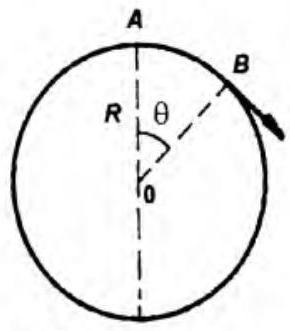
\includegraphics[max width=\textwidth, center]{2025_07_01_5b3ff9fa0d508c8e9f17g-057(1)}

Fig. 1.20\\
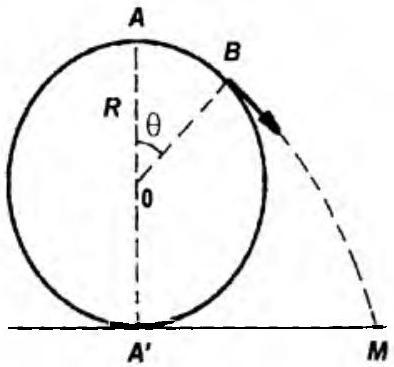
\includegraphics[max width=\textwidth, center]{2025_07_01_5b3ff9fa0d508c8e9f17g-057}

Fig. 1.21

1.251.*O bandă circulară de masă $m$ şi rază $r$ se rotește în jurul unei axe -ご:le care trece prin centru,perpendiculară pe planul benzii,astfel încât fiecare murc:are viteza $v$ .Calculați tensiunea din bandă,presupunând că aceasta este ne:二〇- 7 sibilă.\\
ㅅ.$T=\frac{m v^{2}}{\pi r^{2}}$ ;\\
B)$T=\frac{m v^{2}}{2 \pi r}$ ;\\
C)$T=\frac{m v^{2}}{r}$ ;\\
D.$T=\frac{m v^{2}}{2 r}$ ;\\
E)$T=\frac{m v^{2}}{2}$ ;\\
F)$T=\frac{m v}{r}$ .\\
(Alexandrina Nenciu)\\
1.252.*Într-un parc de distracții maşinile se 2.三eazã pe o buclă verticală,conform Fig.1.22.Dacă n :z-:aa superioară bucla este un cerc de rază $R=10 \mathrm{~m}$ -உ--crul cel mai înalt se află la înălțimea $h=30 \mathrm{~m}$ de $\therefore$ :are este viteza minimă cu care trebuie să intre пац-$=\equiv$ in buclă,pentru a nu cădea.\\
A. $50 \mathrm{~m} / \mathrm{s}$ ;\\
B) $23 \mathrm{~m} / \mathrm{s}$ ;\\
C) $10 \mathrm{~m} / \mathrm{s}$ ;\\
D) $26,1 \mathrm{~m} / \mathrm{s}$ ;E) $\mathrm{s}=-\mathrm{s}$ :F) $100 \mathrm{~m} / \mathrm{s}$ .\\
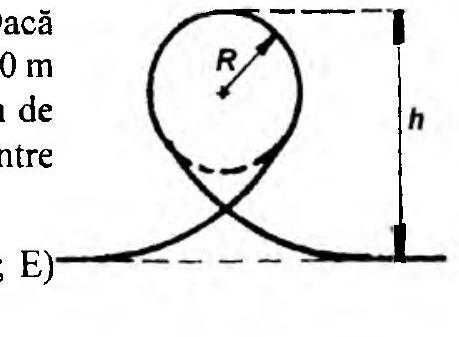
\includegraphics[max width=\textwidth, center]{2025_07_01_5b3ff9fa0d508c8e9f17g-057(2)}

Fig. 1.22\\
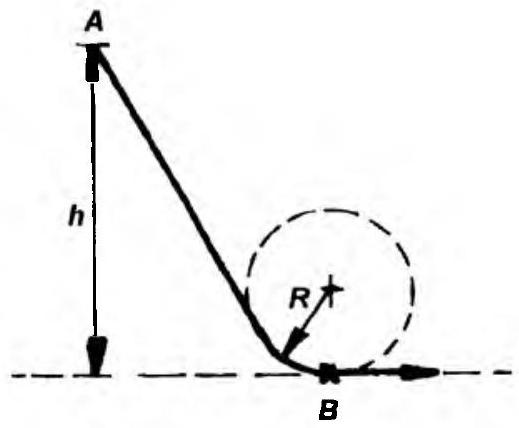
\includegraphics[max width=\textwidth, center]{2025_07_01_5b3ff9fa0d508c8e9f17g-058(1)}

Fig. 1.23\\
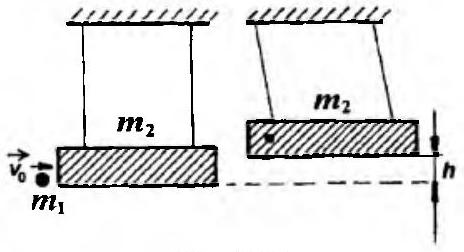
\includegraphics[max width=\textwidth, center]{2025_07_01_5b3ff9fa0d508c8e9f17g-058}

Fig. 1.24\\
1.253.* Într-un parc de distracții, maşinile alunecă de la înălțimea $h=50 \mathrm{~m}$, pe o curbă ca în Fig. 1.23. Dacă pasagerii suportă o accelerație egală cu $8 g$, care trebuie să fie raza $R$ a cercului de la baza curbei?\\
A) 50 m ;\\
B) 3 m ;\\
C) $7,2 \mathrm{~m}$;\\
D) $14,3 \mathrm{~m}$;\\
E) $50,2 \mathrm{~m}$;\\
F) $17,2 \mathrm{~m}$.\\
(Alexandrina Nenciu)\\
1.254.* Una din metodele de măsurare a vitezei proiectilelor constă în folosirea unui pendul balistic. Acesta este un corp de lemn de masă $m_{2}$, suspendat cu ajutorul a două fire lungi (Fig. 1.24). Inițial pendulul este în repaus. Un proiectil de masă $m_{1}$ loveşte orizontal corpul din lemn și rămâne încastrat, făcând ca pendulul şi proiectilul sã se ridice la înălțimea $h$. Dacă masa pendulului este $m_{2}=4 \mathrm{~kg}$, masa proiectilului este $m_{1}=9,7 \mathrm{~g}$ şi în urma impactului se ridică la $h=19 \mathrm{~cm}$, care este viteza inițială a proiectilului ? ( $g=9,8 \mathrm{~m} / \mathrm{s}^{2}$ )\\
A) $10 \mathrm{~m} / \mathrm{s}$;\\
B) $256 \mathrm{~m} / \mathrm{s}$;\\
C) $1452 \mathrm{~m} / \mathrm{s}$;\\
D) $3452 \mathrm{~m} / \mathrm{s}$;\\
E) $960 \mathrm{~m} / \mathrm{s}$;\\
F) $798 \mathrm{~m} / \mathrm{s}$.\\
(Alexandrina Nenciu)\\
1.255.* $\varnothing$ piatră aruncată pe orizontală cu viteza $v_{0}=15 \mathrm{~m} / \mathrm{s}$ de pe acoperişul unei case, cade pe sol sub unghiul $\alpha=60^{\circ}$ față de orizontală. Care este înălțimea $h$ a casei ? ( $g=9,8 \mathrm{~m} / \mathrm{s}^{2}$ )\\
A) $30,3 \mathrm{~m} / \mathrm{B}$\\
B) $34,4 \mathrm{~m}$;\\
C) $36,1 \mathrm{~m}$;\\
D) $39,2 \mathrm{~m}$;\\
E) 35 m ;\\
F) 28 m .\\
(George Ionescu)\\
1.256.* Un automobil trece peste un pod convex cu viteza $v=72 \mathrm{~km} / \mathrm{h}$. Să se calculeze raza de curbură a podului la mijlocul acestuia, știind ca în acest punct automobilul apasă cu o forță egală cu $4 / 5$ din greutatea sa. Se va aproxima $g=10 \mathrm{~m} / \mathrm{s}^{2}$.\\
A) 180 m ;\\
B) 200 m ;\\
C) 240 m ;\\
D) 270 m ;\\
E) 320 m ;\\
F) 254 m .\\
1.257.* De pe vârful unei sfere de rază $R=3 \mathrm{~m}$ alunecă liber în jos, fără tés inițială, un mic corp. La ce înălțime de vârful sferei se va desprinde corpul ? - $\lambda 0,5 \mathrm{~m}$; B) $0,7 \mathrm{~m}$; C) 1 m ; D) $1,2 \mathrm{~m}$; E) $1,3 \mathrm{~m}$; F) $1,5 \mathrm{~m}$.\\
(George Ionescu)\\
1.258. Un om deplasează uniform, pe un drum drept şi orizontal, o sanie cu naż de 50 kg , trăgând-o cu o forță constantă de 300 N prin intermediul unui fir IL - -3 t cu $30^{\circ}$ faţă de orizontală. Calculați valoarea coeficientului de frecare. $z=9.8 \mathrm{~m} / \mathrm{s}^{2}$ )

$$
\text { A। } 0,55 \text {; B) } 0,63 \text {; C) } 0,91 \text {; 万) } 0,76 \text {; E) } 0,85 \text {; F) } 0,38 \text {. }
$$

(George Ionescu)\\
1.259. Cu câți kW lucrează o locomotivă care dezvoltă o forță de tracțiune de $\because$ \% N şi remorchează un tren ce se deplasează cu $54 \mathrm{~km} / \mathrm{h}$ ?\\
A) 260 kW ;\\
B) 300 kW ;\\
C) 370 kW ;\\
D) 450 kW ;\\
E) 560 kW ;\\
F) 415 kW .\\
(George Ionescu)\\
1.260. Pentru ca un automobil să se deplaseze cu viteza de $30 \mathrm{~m} / \mathrm{s}$, motorul realtă o putere de $6 \cdot 10^{4} \mathrm{~W}$. Ce distantặ poate parcurge automobilul cu 1 litru de zízină, ştiind că energia furnizată de acesta motorului este de $8 \cdot 10^{6} \mathrm{~J} / l$.\\
A) 3 km ;\\
B) $3,5 \mathrm{~km}$;\\
C) 4 km ;\\
D) $4,5 \mathrm{~km}$;\\
E) 6 km ; F) $7,2 \mathrm{~km}$.\\
(George Ionescu)\\
1.261. Pentru a atinge viteza de regim pornind din repaus pe un drum : zontal, un camion este supus un timp $t=10 \mathrm{~s}$ acțiunii unei forțe de tractiune ${ }^{-}=6 \mathrm{kN}$, care efectuează în acest interval un lucru mecanic $L=600 \mathrm{~kJ}$. Să se玨uleze accelerația imprimată camionului.\\
A) $1 \mathrm{~m} / \mathrm{s}^{2}$;\\
B) $2 \mathrm{~m} / \mathrm{s}^{2}$;\\
C) $3 \mathrm{~m} / \mathrm{s}^{2}$;\\
D) $4 \mathrm{~m} / \mathrm{s}^{2}$;\\
E) $5 \mathrm{~m} / \mathrm{s}^{2}$;\\
F) $2,5 \mathrm{~m} / \mathrm{s}^{2}$.\\
(George Ionescu)\\
1.262. Cu ce forţă minimă orizontală trebuie să acționăm asupra unui corp de - 3 ăa $m=1 \mathrm{~kg}$, ce se află pe un plan înclinat de unghi $\alpha=30^{\circ}$, pentru ca corpul să Enână în repaus? Se dau $\mu=0,2 ; g=10 \mathrm{~m} / \mathrm{s}^{2}$.\\
A) $5,02 \mathrm{~N}$;\\
B) 11 N ;\\
C) $3,77 \mathrm{~N}$;\\
D) $1,78 \mathrm{~N}$;\\
E) 4,03;\\
F) $2,15 \mathrm{~N}$.\\
(George Ionescu)\\
1.263.* O bilă de masă $m=2 \mathrm{~kg}$ este suspendată de un fir de lungime $=0,4 \mathrm{~m}$. Se imprimă bilei o mişcare de rotație uniformă în planul orizontal\\
(pendul conic) cu viteza unghiulară $\omega=7 \mathrm{rad} / \mathrm{s}$. Să se calculeze energia cinetică a bilei.\\
A) $7,3 \mathrm{~J}$;\\
В) $5,8 \mathrm{~J}$;\\
C) $9,5 \mathrm{~J}$;\\
D) $4,7 \mathrm{~J}$;\\
E) $9,8 \mathrm{~J}$;\\
F) $8,3 \mathrm{~J}$.\\
(George Ionescu)\\
1.264.* Un obiect, aruncat sub unghiul $\alpha=30^{\circ}$ fațā de orizontală se află la aceeaşi înălțime $h$ la două momente diferite $t_{1}=3 \mathrm{~s}$ şi $t_{2}=5 \mathrm{~s}$ de la începutul mişcării. Să se determine viteza $v_{0}$ și înălțimea $h$. Se dă $g=10 \mathrm{~m} / \mathrm{s}^{2}$.\\
A) $70 \mathrm{~m} / \mathrm{s}$ şi 68 m ;\\
B) $80 \mathrm{~m} / \mathrm{s}$ şi 75 m ; C) $90 \mathrm{~m} / \mathrm{s}$ şi 82 m ;\\
D) $78 \mathrm{~m} / \mathrm{s}$ şi 102 m ;\\
E) $45 \mathrm{~m} / \mathrm{s}$ şi $\mathbf{8 0 ~ m}$; F) $73 \mathrm{~m} / \mathrm{s}$ şi $\mathbf{9 0 ~ m}$.\\
(George Ionescu)\\
1.265. Un pendul format dintr-un fir de lungime $l=1,6 \mathrm{~m}$ și o bilă de masă $m=0,5 \mathrm{~kg}$ aflat în poziție de repaus, primeşte un impuls $p=2 \mathrm{~N} \cdot \mathrm{~s}$. Să se calculeze unghiul maxim pe care îl face firul cu poziția de echilibru.\\
А) $30^{\circ}$;\\
B) $45^{\circ}$;\\
C) $60^{\circ}$,\\
D) $75^{\circ}$;\\
E) $90^{\circ}$; F) $180^{\circ}$.\\
(George Ionescu)\\
1.266. Ce viteză inițială i se imprimă unui obuz lansat sub unghiul $\alpha=30^{\circ}$ pentru a cădea la distanța $d=17300 \mathrm{~m}$ ? Se aproximează $g=10 \mathrm{~m} / \mathrm{s}^{2}$; se neglijează rezistența aerului.\\
(A) $446 \mathrm{~m} / \mathrm{s}$;\\
B) $495 \mathrm{~m} / \mathrm{s}$;\\
C) $502,1 \mathrm{~m} / \mathrm{s}$;\\
D) $385 \mathrm{~m} / \mathrm{s}$;\\
E) $324 \mathrm{~m} / \mathrm{s}$; F) $523 \mathrm{~m} / \mathrm{s}$.\\
(George Ionescu)\\
1.267.* De un lanţ rigid, ce rezistă la o tensiune maximă $T_{\max }=40 \mathrm{~N}$, este suspendat un corp cu masa $m=1 \mathrm{~kg}$. Care este unghiul pe care îl poate face lanţul cu poziția de echilibru, astfel ca lanțul să nu se rupă în timpul oscilației ?\\
А) $75^{\circ}$;\\
в) $90^{\circ}$,\\
C) $110^{\circ}$,\\
D) $120^{\circ}$,\\
E) $60^{\circ}$;\\
F) $45^{\circ}$.\\
(George Ionescu)\\
1.268. Pe un plan înclinat de unghi $\alpha=30^{\circ}$ se află un corp de masă $m=50 \mathrm{~kg}$, asupra căruia actionează o forță orizontală $F=294 \mathrm{~N}$ (Fig. 1.25). Neglijând frecările, să se calculeze accelerația cu care se mişcă corpul şi forța cu care apasă asupra planului. ( $g=10 \mathrm{~m} / \mathrm{s}^{2}$ )\\
A) $12,1 \mathrm{~m} / \mathrm{s}^{2}$ şi $360,3 \mathrm{~N}$;\\
B) $9 \mathrm{~m} / \mathrm{s}^{2}$ şi $382,5 \mathrm{~N}$;\\
C) $10,1 \mathrm{~m} / \mathrm{s}^{2}$ şi $285,5 \mathrm{~N}$;\\
D) $8 \mathrm{~m} / \mathrm{s}^{2}$ şi 422 N ;\\
E) $7,5 \mathrm{~m} / \mathrm{s}^{2}$ şi 324 N ;\\
F) $8,7 \mathrm{~m} / \mathrm{s}^{2}$ şi 385 N .\\
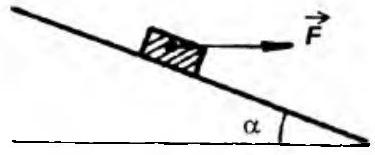
\includegraphics[max width=\textwidth, center]{2025_07_01_5b3ff9fa0d508c8e9f17g-061(1)}

Fig. 1.25\\
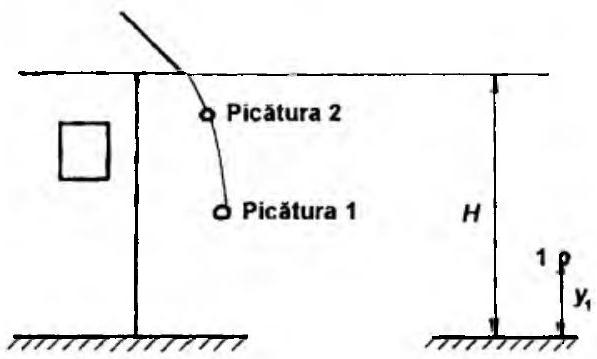
\includegraphics[max width=\textwidth, center]{2025_07_01_5b3ff9fa0d508c8e9f17g-061(2)}

Fig. 1.26

1.269.De pe un acoperiş cad,una după alta,două picături de apă(Fig.1.26). --ạa un timp $\tau=2 \mathrm{~s}$ de la începutul căderii celei de-a doua picături,distanța二:-e ele este $\Delta h=25 \mathrm{~m}$ .Cu cât timp înaintea desprinderii celei de-a doua こ心äturi s-a desprins prima picătură de pe acoperiş ?\\
A) 3 s ;B) 7 s ;\\
C) 1 s ;\\
D) $0,7 \mathrm{~s}$ ;\\
E) $1,8 \mathrm{~s}$ ;F) $2,4 \mathrm{~s}$ .\\
(George Ionescu)\\
1.270.Un teleschi funcționeazǎ pe o pantă de 240 m ,înclinatǎ la $30^{\circ}$ .Cablul *Jeplasează cu $10 \mathrm{~km} / \mathrm{h}$ şi trage simultan 100 schiori,cu o masă medie de 72 kg . ミstimați puterea necesară pentru funcționarea teleschiului.(Se neglijează二izarea).$\left(g=9,8 \mathrm{~m} / \mathrm{s}^{2}\right)$\\
A) $1000 \mathrm{~J} / \mathrm{s}$ ;\\
B) 49000 W ;\\
C) 100 kW ;\\
D) $0,1 \mathrm{GW}$ ;\\
E) $50 \mathrm{~kJ} / \mathrm{h}$ ;\\
F) 98 kW .\\
(Ionuț Puică)\\
1.271 Ce accelerație trebuie să aibă căruciorul din F. 1.27 astfel încât corpul A să nu cadă ?Coeficientul :e frecare dintre corp şi cărucior este $\mu$ .

A)mai mare sau egală cu $g / \mu ; \mathbf{B}) g ;$ C)$\mu g$ ;\\
D)infinită;E)problema nu are soluție;F)$g / \mu$ .\\
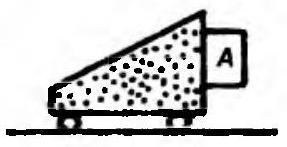
\includegraphics[max width=\textwidth, center]{2025_07_01_5b3ff9fa0d508c8e9f17g-061}

Fig. 1.27\\
(Ionuț Puică)\\
1.272.*Un vagon descoperit de cale ferată cu masa de 10 t alunecă fără Fecare de-a lungul unor şine orizontale.Plouă puternic,ploaia căzând vertical. Vagonul este inițial gol şi se mişcă cu o viteză de $1 \mathrm{~m} / \mathrm{s}$ .Care este viteza vagonului jupă ce s-a deplasat suficient pentru a strânge 1000 kg de apă de ploaie ?\\
A) $0,91 \mathrm{~m} / \mathrm{s}$ ;\\
B) $0,5 \mathrm{~m} / \mathrm{s}$ ;\\
C)zero;\\
D) $10 \mathrm{~cm} / \mathrm{s}$ ;\\
E) $8 \mathrm{dm} / \mathrm{s}$ ;\\
F) $10 \mathrm{~km} / \mathrm{h}$ .\\
(1.273. Un ascensor şi încărcătura lui au o masă totală de 800 kg . Să se determine tensiunea $T$ din cablul de susținere atunci când ascensorul, care se mişcă inițial în jos cu $10 \mathrm{~m} / \mathrm{s}$, este oprit cu accelerație constantă pe o distantă de 25 m . ( $g=9,8 \mathrm{~m} / \mathrm{s}^{2}$ )\\
(A) 9440 N ; B) 7840 N ; C) 1600 N ; D) egală cu greutatea ascensorului;\\
E) nu se poate calcula din datele problemei; F) 6240 N .\\
(Ionuț Puică)\\
1.274. Motorul unei bărci furnizează elicei o putere de 30 kW atunci când barca se deplasează cu o viteză de $30 \mathrm{~km} / \mathrm{h}$. Care ar fỉ tensiunea din cablu, dacă barca ar fi remorcată cu aceeaşi viteză ?\\
A) 1000 N ; B) 49 kN ; C) 3600 N ; D) $0,1 \mathrm{GN}$; E) 50 kN ; F) 98 N .\\
(Ionuț Puică)\\
1.275.* O minge de greutate $G$ este legată de o coardã şi pusă în mişcare de rotație pe un cerc vertical. Tensiunea din coardă în punctul cel mai de jos este mai mare decât cea din punctul cel mai înalt cu o valoare egală cu:\\
A) depinde de viteza de rotație; B) tensiunile sunt egale; C) $G$;\\
D) $6 G$; E) $2 G$; F) depinde de lungimea corzii.\\
(Ionuț Puică))\\
1.276. Două trenuri aflate în mişcări rectilinii paralele uniform accelerate, în același sens, se reîntâlnesc după 14 s de la depășire. După cât timp de la prima depăşire trenurile vor avea aceeaşi viteză instantanee?\\
A) 20 s ; B) 10 s ; C) 1 min ; D) 5 s ; E) 7 s ; F) $9,8 \mathrm{~s}$.\\
(Radu Chişleag)\\
1.277. Un cart, cu masa totală de 100 kg , parcurge uniform o rampă lungă de $3,6 \mathrm{~km}$, în 4 min şi 5 s . La fiecare tură de roată cu o lungime de 180 cm , centrul său de masă urcă cu 5 cm . Care este puterea consumată de cart neglijând rezistența aerului şi frecarea cu solul ? Se cunoaşte: $g=9,8$ u.S.I.\\
A) $0,8 \mathrm{kWh}$;\\
B) 400 J ;\\
C) 400 W ;\\
D) 500 Wh ;\\
E) $0,4 \mathrm{kWh}$;\\
F) 500 J .

1.278.Un om având înălțimea $h=180 \mathrm{~cm}$ se deplasează cu viteza $=2 \mathrm{~ms}^{-1}$ ,trecând pe sub un felinar situat la înălțimea de $5,4 \mathrm{~m}$ .Cu ce viteză $V$ $\approx$ ungeşte umbra omului pe sol?\\
A) $2 \mathrm{~ms}^{-1}$ ;\\
B) $6 \mathrm{~ms}^{-1}$ ;\\
C) $4 \mathrm{~m} / \mathrm{s}$ ;\\
D) $5,4 \mathrm{~km} / \mathrm{h}$ ;\\
E) $7,5 \mathrm{~m} / \mathrm{s}$ ;\\
F) $3 \mathrm{~m} / \mathrm{s}$ .\\
(Radu Chişleag)\\
1.279.Un leu cu greutatea de 980 N se mişcă accelerat,din repaus până la -き和 de $36 \mathrm{~km} / \mathrm{h}$ ,în $1,25 \mathrm{~s}$ .Care a fost puterea medie necesară pentru această ผ:こそerare,neglijând frecările?\\
A) 10 kW ;\\
B) 5 kW ;\\
C) 2 kW ;\\
D) 50 kJ ;\\
E) 4 kW ;F) 4 kJ .\\
(Radu Chişleag)\\
1.280.O şopârlă se află într-un colț de jos al unei cutii cubice transparente cu æга de 200 cm şi își vede puiul agățat în colțul opus de sus,al cutiei.Care este $\because$ nai scurt timp în care puiul nemişcat poate primi ajutorul mamei,dacă mama $\leftarrow$ zvate deplasa pe suprafața cutiei în orice direcție,cu viteza de $10 \mathrm{~cm} / \mathrm{s}$ ?

A)nu se poate rezolva cu datele din problemă;\\
B) 2 min şi 3 s ;\\
C) 447 s ;\\
D) $89,4 \mathrm{~s}$ ;\\
E) 67 s ;F) 2 şi $3 / 4$ .\\
(Radu Chişleag)\\
1.281.Doi prieteni $E l$ şi $E a$ se aflã la distanta de 100 m unul de altul,pe o :--tie paralelă cu un zid.Apelul Lui este auzit de $E a$ ,de 2 ori,la un interval de -$=100 \mathrm{cs}$ .Să se determine distanta dintre prieteni şi zid,dacă viteza sunetului în este de $340 \mathrm{~m} / \mathrm{s}$ .\\
A) 270 m ;\\
B) 185 m ;\\
C) 214 m ;\\
D) 60 m ;\\
E) 107 m ;\\
F) 120 m .\\
(Radu Chişleag)\\
1.282.Ce fortă medie este necesară pentru a frâna un cărucior în 5 s ,dacă Zulsul acestuia,înaintea frânării este de $100 \mathrm{~kg} \cdot \mathrm{~m} \cdot \mathrm{~s}^{-1}$ ?\\
A) $5 \mathrm{~m} / \mathrm{s}$\\
(B) 20 N ;\\
C) $100 \mathrm{~kg} \cdot \mathrm{~m} \cdot \mathrm{~s}^{-1}$ ;\\
D) 5 kN ;\\
E) 40 kN ;\\
F) 20 kN .\\
(Radu Chişleag)\\
1.283.Un tren parcurge prima jumătate a distanței Bucureşti-Alexandria cu -:こza $v_{1}$ ,iar restul traseului cu viteza $v_{2}=21,6 \mathrm{~km} / \mathrm{h}$ .Dacă viteza medie pe ==eaga distantă a fost $v_{m}=10 \mathrm{~ms}^{-1}$ ,care este $v_{1}$ ?\\
A) $21,6 \mathrm{~km} / \mathrm{h}$ ;\\
B) $30 \mathrm{~m} / \mathrm{s}$ ;\\
C) $54 \mathrm{~km} / \mathrm{h}$ ;\\
D) $36 \mathrm{~m} / \mathrm{s}$ ;\\
E) $20 \mathrm{~m} / \mathrm{s}$ ;\\
F) $14 \mathrm{~m} / \mathrm{s}$ .\\
1.284.* Care trebuie să fie raza minimă a pistei circulare a unui velodrom improvizat plan pe care se deplasează cicliştii, cu $54 \mathrm{~km} / \mathrm{h}$, dacă coeficientul de frecare la alunecare laterală al roților bicicliştilor este $\mu=0,5 ?\left(g=9,8 \mathrm{~m} / \mathrm{s}^{2}\right)$\\
A) 60 m ;\\
B) 408 dm ;\\
C) 54 m ;\\
D) 508 dm ;\\
E) 459 dm ;\\
F) 64 m .\\
(Radu Chişleag)\\
1.285. Un elicopter parcurge într-o regiune cu vânt constant de direcția AB , la înălțimea de zbor de 1 km , traseul AB în 50 min şi traseul invers, BA , în 70 min . În cât timp ar parcurge traseul BA , un balon care ar pluti la aceeaşi înălțime cu avionul?\\
A) 60 min ;\\
B) 120 min ;\\
C) balonul nu poate parcurge traseul BA ;\\
D) 24 ore;\\
E) 350 min ;\\
F) 3 zile.\\
(Radu Chişleag)\\
1.286. Un tren cu masa $M=440 \mathrm{t}$ se deplasează uniform şi rectiliniu, cu viteza $\downarrow=36 \mathrm{~km} / \mathrm{h}$, având coeficientul de frecare $\mu=0,05$. La un moment dat se desprinde ultimul vagon, cu masa $m=40000 \mathrm{~kg}$. Dacă $F_{t}$, forța de tracțiune se menține constantă, care soluție descrie mişcarea trenului imediat după desprinderea vagonului ?\\
(A) $a=0,049 \mathrm{~ms}^{-2} \quad v=10 \mathrm{~ms}^{-1} ;$\\
B) $v=9,8 \mathrm{~m} / \mathrm{s}$;\\
C)\\
$a=0,098 \mathrm{~m} / \mathrm{s}$;\\
D) $a=-0,049 \mathrm{~ms}^{-2}$;\\
E) $a=0,98 \mathrm{~m} / \mathrm{s}^{2}$;\\
F)\\
$a=0,098 \mathrm{~ms}^{-2}$.\\
(Radu Chişleag)\\
1.287. Un lift, care se deplasează pe verticală cu viteza constantă de $11 \mathrm{~m} / \mathrm{s}$, pierde o piuliță la înălțimea de 16 m . Cu cât va fí mai mare viteza piuliței la contactul cu solul în cazul în care liftul ar fi în coborâre decât în cazul că acesta ar fi în urcare, neglijând frecările?\\
A) 0 ; B) $4 \mathrm{~m} / \mathrm{s}$; C) $21 \mathrm{~m} / \mathrm{s}$; D) $11 \mathrm{~m} / \mathrm{s}$; E) $-21 \mathrm{~m} / \mathrm{s}$; F) $-4 \mathrm{~m} / \mathrm{s}$.\\
(Radu Chişleag)\\
1.288. O coardă elastică, folosită la o întrecere de forță de tracțiune între doi jucători de forțe egale, se alungeşte, prin tragere, cu distanța $\Delta L_{1}=4 \mathrm{~cm}$. Dacã

Levași bucată de fir este pusă în două,care va fi modificarea distanței,$\Delta L_{2}$ , $\simeq-\mathrm{z}_{-}$aceiaşi jucători,prin tragere,cu aceleaşi forțe ?\\
A) $5 \cdot 10^{-3} \mathrm{~m}$ ;\\
B) 1 cm ;\\
C) 8 cm ;\\
D) $0 ;$ E) $4 \mathrm{~cm} ;$ F) 2 cm .\\
(Radu Chişleag)\\
1.289.Un glonț este lansat pe verticală,cu viteza inițială de $144 \mathrm{~km} / \mathrm{h}$ .Cu cât в rește inălțimea maximă atinsă,dacă viteza inițială s-ar tripla ?Se consideră $s=10 \mathrm{~m} / \mathrm{s}^{2}$ .\\
A) 2400 dm ;\\
B) 120 m ;\\
C) 120 dm ;\\
D) 640 m ;\\
E) 1240 dm ;\\
F) 144 m .\\
(Radu Chişleag)\\
1.290.O alice,cu masa de 1 g ,intră orizontal într-un bloc de lemn de grosime $\ldots$ cu viteza de $100 \mathrm{~m} / \mathrm{s}$ şi iese cu viteza de $600 \mathrm{dm} / \mathrm{s}$ ,fiind frânată uniform.Ce E::ime de lemn ar fi necesară pentru ca alicea să fie reținută ?\\
A) 3 dm ;\\
B) 25 cm ;\\
C) $2,86 \mathrm{dm}$ ;\\
D) 16 cm ;\\
E) $2,86 \mathrm{~cm}$ ;\\
F) $14,3 \mathrm{~cm}$ .\\
(Radu Chişleag)

1.291.Un râu curge spre nord cu o viteză de $4 \mathrm{~m} / \mathrm{s}$ .Un om traversează râul cu :ここ、こа.viteza relativă a bărcii față de apă fiind de $3 \mathrm{~m} / \mathrm{s}$ în directia est.\\
a)Care este viteza relativă a bărcii față de mal ?\\
b)Dacă râul are o lățime de 600 m ,la ce distanță față de punctul de pornire, -三urată pe directia nord,va ajunge barca pe malul opus?\\
A)a) $5 \mathrm{~m} / \mathrm{s}$ ;\\
b) 1 km ;\\
B)a) $7 \mathrm{~m} / \mathrm{s}$ ;\\
b) 800 m ;\\
C)a) $1 \mathrm{~m} / \mathrm{s}$ ;\\
b) 1 km ;\\
D)a) $7 \mathrm{~m} / \mathrm{s}$ ;\\
b) 1 km ;\\
E)a) $5 \mathrm{~m} / \mathrm{s}$ ;\\
b) 800 m ;\\
F)a) $1 \mathrm{~m} / \mathrm{s}$ ;\\
b) 800 m\\
(Mădălina Puică)\\
1.292 Un corp cu masa $m_{1}=12 \mathrm{~kg}$ aflat în repaus pe o suprafață orizontală ここ)égat printr-o coardă ce trece peste un scripete uşor fără frecări,de un corp cu こここ、 $m_{2}=5 \mathrm{~kg}$ .Coeficientul de frecare dintre primul corp şi suprafaţa orizonatală $\approx \mu=0,5$ .Determinați:a)tensiunea $T$ din coardă;b)accelerația $a$ a squrilor.\\
A)a) 40 N ;\\
b) $2 \mathrm{~m} / \mathrm{s}^{2}$ ;\\
(B)a) 49 N ;\\
b) $0 \mathrm{~m} / \mathrm{s}^{2}$ ;\\
C)a) 50 N ;\\
b) $5 \mathrm{~m} / \mathrm{s}^{2}$ ;\\
D)a) 20 N ;\\
b) $1 \mathrm{~m} / \mathrm{s}^{2}$ ;\\
E)a) 49 N ;\\
b) $1 \mathrm{~m} / \mathrm{s}^{2}$ ;\\
F)a) 100 N ;\\
b) $0 \mathrm{~m} / \mathrm{s}^{2}$ .\\
1.293. Un automobil accelerează de la $36 \mathrm{~km} / \mathrm{h}$ la $82,8 \mathrm{~km} / \mathrm{h}$ în 13 s . Calculați accelerația şi distanța parcursă de automobil în acest timp, presupunând că accelerația e constantă.\\
A) $1 \mathrm{~cm} / \mathrm{s}^{2}$ şi 200 m ; B) $0,5 \mathrm{~m} / \mathrm{s}^{2}$ şi $214,5 \mathrm{~m}$; C) $1,5 \mathrm{~m} / \mathrm{s}^{2}$ şi $2,5 \mathrm{~km}$;\\
D) $1 \mathrm{~m} / \mathrm{s}^{2}$ şi 2 km ; E) $0,1 \mathrm{~km} / \mathrm{h}^{2}$ şi $0,25 \mathrm{~km}$; F) $1 \mathrm{~m} / \mathrm{s}^{2}$ şi $214,5 \mathrm{~m}$.\\
(Mădălina Puică)\\
1.294. O locomotivă tractează două vagoane. Masa locomotivei este de $M=6 t$, lar masa fiecărui vagon este de $m=2 t$. Trenul pleacă din repaus, cu accelerația de $0,5 \mathrm{~m} / \mathrm{s}^{2}$. Determinați tensiunile din sistemul de cuplaj dintre locomotivă şi primul vagon, şi dintre cele două vagoane.\\
A) 2000 N in ambele cuplaje;\\
B) 1 kN şi $0,5 \mathrm{kN}$;\\
C) 2000 N şi 1000 N ;\\
D) 1000 N şi 500 N ;\\
E) 1000 N in ambele cuplaje;\\
F) 2000 N şi zero.\\
(Mădălina Puică)\\
1.295. O bară având lungimea inițială $L$, aria secțiunii transversale $S$ şi modulul lui Young $E$, este supusă unei forte de tensiune $F$. Notăm efortul unitar în bară prin $\sigma=\frac{F}{S}$, iar alungirea relativă prin $\varepsilon=\frac{\Delta L}{L}$. Deduceți expresia energiei potențiale elastice din unitatea de volum a barei, $w=\frac{E_{p}}{L \cdot S}$, în funcţie de $\sigma$ şi $\varepsilon$.\\
A) $\varepsilon^{2} / 2$;\\
B) $\varepsilon \sigma$;\\
C) $\sigma^{2} / E$;\\
D) $\sigma / \varepsilon$;\\
E) $\varepsilon \sigma / 2$;\\
F) $\varepsilon^{2} \sigma$.\\
(Mădălina Puică)\\
1.296.* Scala unui dinamometru, care indică valori de la 0 la 180 N , are lungimea de 9 cm . Se observă că un corp suspendat de dinamometru oscilează vertical cu $1,5 \mathrm{~Hz}$. Care este masa corpului ? Masa arcului se neglijează.\\
A) 10 kg ;\\
B) $22,5 \mathrm{~kg}$;\\
C) 200 g ;\\
D) 45 kg ;\\
E) $9,8 \mathrm{~kg}$;\\
F) 180 kg .\\
(Mădălina Puică)\\
1.297.* Un corp cu masa $m_{1}=0,1 \mathrm{~kg}$ alunecă pe un plan înclinat cu $\alpha=45^{\circ}$, de lungime $l=2 \mathrm{~m}$. La baza planului corpul ciocneşte perfect plastic un corp cu masa $m_{2}=3 m_{1}$, legat de un resort inițial necomprimat, având constanta de elasticitate $k=800 \mathrm{~N} / \mathrm{m}$. Ştiind că cele două corpuri pleacă împreună pe orizontală iar coeficientul de frecare, acelaşi, atât pe planul înclinat cât şi pe orizontală este $\mu=0,8$, aflați cu cât se comprimă resortul ( $g \cong 10 \mathrm{~m} / \mathrm{s}^{2}$ ).\\
A) 2 cm ;\\
B) 1 cm ;\\
C) $0,5 \mathrm{~cm}$;\\
D) $1,5 \mathrm{~cm}$; E) 1 mm ;\\
F) 5 mm .

1.298.Un mobil în mişcare uniform accelerată parcurge o distantă $d=125 \mathrm{~m}$ , - 2 sa crescând de la $N_{1}=18 \mathrm{~km} / \mathrm{h}$ la $N_{2}=72 \mathrm{~km} / \mathrm{h}$ .Ştiind că puterea aroului este $P=15 \mathrm{~kW}$ ,ce lucru mecanic s-a efectuat in acest proces?\\
A) 150 J ;\\
B) 2 kJ ;\\
C) 150 kJ ;\\
D) 200 kJ ;\\
E) 100 kJ ;\\
F) 15 kJ .\\
(Rodica Bena)\\
1.299.*Un vagon netractat cu masa $m_{1}$ parcurge pe orizontală o distantă s $=600 \mathrm{~m}$ ,viteza sa scăzând la jumătate.În acest moment el ciocneşte plastic un En cu masa $m_{2}$ ,aflat în repaus.Ştiind că ansamblul celor două vagoane гæг:urge până la oprire distanța $d_{2}=50 \mathrm{~m}$ ,aflați raportul $n=\frac{m_{2}}{m_{1}}$ al maselor celor בי.工. 3 vagoane.Coeficientul de frecare este acelasi pe tot parcursul.\\
A)$n=1$ ;\\
B)$n=2$ ;\\
C)$n=1,5$ ;\\
D)$n=2,5$ ;\\
F)$n=2 / 3$ .\\
(Rodica Bena)\\
1.300.Un corp are energia cinetică $E_{c}=200 \mathrm{~J}$ .Lucrul mecanic efectuat Eña corpului pentru a-i mări impulsul de 4 ori este:\\
A) 800 J ;\\
B) 1600 J ;\\
C) 2 kJ ;\\
D) 3 kJ ;\\
E) $3,2 \mathrm{~kJ}$ ;F) 600 J .\\
(Rodica Bena)\\
1.301.Alegeți expresia corectã pentru uniattea de măsură a randamentului:\\
A)W;\\
B) $\mathrm{J} \cdot \mathrm{s}$ ;\\
C)$\frac{\mathrm{J} \cdot \mathrm{s}}{\mathrm{Kg} \cdot \mathrm{m}}$ ;\\
D)$\frac{\mathrm{J} \cdot \mathrm{s}^{2}}{\mathrm{Kg} \cdot \mathrm{m}^{2}}$ ;\\
E)$\frac{\mathrm{N} \cdot \mathrm{m}}{\mathrm{J} \cdot s}$ ;F)J.\\
(Rodica Bena)\\
1.302.Un mobil se deplasează pe orizontală,având ecuația de mişcare s.:$)=100+20 t-t^{3}$ .Aflați viteza medie a mobilului între secunda a H-a şi ミン: 1 Inda a III-a.

A) $1 \mathrm{~m} / \mathrm{s}$ ;B)$-1 \mathrm{~m} / \mathrm{s}$ ;C)$-15 \mathrm{~m} / \mathrm{s}$ ;D) $0,5 \mathrm{~m} / \mathrm{s}$ ;E) $2 \mathrm{~m} / \mathrm{s}$ ;F)$-0,5 \mathrm{~m} / \mathrm{s}$ .\\
(Rodica Bena)\\
1.303.Alegeți afirmația incorectă:A)Forța de frecare de alunecare apare la s-prafața de contact a două corpuri în mişcare de alunecare relativă.B)Forța de -zare statică apare la suprafața de contact între două corpuri.C)Forța de frecare i:exercitã asupra ambelor corpuri în contact.D)Forta de frecare de alunecare este -roportională cu suprafața de contact a corpurilor.E)forta de frecare de alunecare ze expresia $f_{f}=\mu N$ ;F)Forta de frecare depinde starea de rugozitate a s.jprafetelor.\\
(Rodica Bena)\\
1.304. Dintr-un punct pleacă din repaus un mobil cu accelerația $a_{1}=2 \mathrm{~m} / \mathrm{s}^{2}$. Din același punct pleacă în acelaşi sens după $\tau=1 s$ un mobil cu viteza $v_{02}$ şi $a_{2}=-2 \mathrm{~m} / \mathrm{s}^{2}$. Ştiind că intervalul de timp între cele două întâlniri succesive ale mobilelor este $\Delta t=0,5 \mathrm{~s}$, să se afle viteza inițială a celui de al doilea mobil.\\
A) $5 \mathrm{~m} / \mathrm{s}$;\\
B) $10 \mathrm{~m} / \mathrm{s}$;\\
C) $20 \mathrm{~m} / \mathrm{s}$;\\
D) $3 \mathrm{~m} / \mathrm{s}$; E) $15 \mathrm{~m} / \mathrm{s}$;\\
F) $2,5 \mathrm{~m} / \mathrm{s}$.\\
(Rodica Bena)\\
1.305. Un camion s-a deplasat din punctul A în punctul B cu $v_{1}=60 \mathrm{~km} / \mathrm{h}$ iar $\operatorname{din} \mathrm{B}$ in A cu $v_{2}=40 \mathrm{~km} / \mathrm{h}$. Viteza medie a camionului a fost:\\
A) $50 \mathrm{~km} / \mathrm{h}$;\\
B) $42 \mathrm{~km} / \mathrm{h}$;\\
C) $55 \mathrm{~km} / \mathrm{h}$;\\
D) $48 \mathrm{~km} / \mathrm{h}$;\\
E) $45 \mathrm{~km} / \mathrm{h}$;\\
F) $100 \mathrm{~km} / \mathrm{h}$.\\
(Rodica Bena)\\
1.306. O locomotivă cu puterea constantă $P$ trage pe un drum orizontal o garnitură de vagoane; trenul are masa totală $m=100 \mathrm{t}$. Ştiind că în momentul în care viteza trenului este $36 \mathrm{Km} / \mathrm{h}$, acceleraţia sa este $a=0,9 \mathrm{~m} / \mathrm{s}^{2}$, coeficientul frecare $\mu=0,01$ iar $g \cong 10 \mathrm{~m} / \mathrm{s}^{2}$, puterea locomotivei este:\\
A) 2 MW ;\\
B) 200 kW ;\\
C) 150 kW ;\\
D) $2,5 \mathrm{MW}$;\\
E) 1 MW ;\\
F) $1,5 \mathrm{MW}$.\\
(Rodica Bena)\\
1.307. Un cărucior este tras prin intermediul unei frângii care face un unghi de $60^{\circ} \mathrm{cu}$ orizontala. La deplasarea căruciorului cu 10 m se efectuează un lucru mecanic $L=5 \mathrm{~kJ}$. Forţa de tracțiune este:\\
A) 100 N ;\\
B) 200 N ;\\
C) 500 N ; 800 N ;\\
E) 1000 N ;\\
F) 2 kN .\\
(Rodica Bena)\\
1.308. Doi patinatori stau în repaus pe gheață. Pentru a se pune în mişcare ei se împing reciproc, alunecând apoi până la oprire. Distanta parcursă de primul patinator până la oprire este cu $44 \%$ mai mare decât cea parucrsă de al doilea. Știind că primul patinator are $m_{1}=50 \mathrm{~kg}$, cel de-al doilea patinator are masa $m_{2}$ :\\
A) 60 kg ;\\
B) 55 kg ;\\
C) 50 kg ;\\
D) 45 kg ;\\
E) 70 kg ;\\
F) 75 kg .\\
(Rodica Bena)\\
1.309. Unitatea de măsură a mărimii fizice egală cu mrw este:\\
A) N ;\\
B) Pa ;\\
C) J ;\\
D) Ns ;\\
E) W ; F) T.\\
(Ioana Ivaşcu)\\
1.310. Ecuația mişcării rectilinii a unui mobil este: $x=6 t^{2}+4 t-5(\mathrm{~m})$. Expresia corectă a legii vitezei acestuia este:\\
A) $v=4+12 t(\mathrm{~m} / \mathrm{s})$\\
B) $v=4-12 t(\mathrm{~m} / \mathrm{s})$\\
C) $v=4+6 t(\mathrm{~m} / \mathrm{s})$\\
D) $v=4-5 t(\mathrm{~m} / \mathrm{s})$\\
E) $v=4+16 t(\mathrm{~m} / \mathrm{s})$\\
F) $v=4-6 t(\mathrm{~m} / \mathrm{s})$

1.311.Legea de mişcare a unui corp lansat cu viteza inițială $v_{0}$ ,de la -rafata Pământului,vertical în sus,neglijând frecările este:\\
A)$y=v_{0} t-\frac{g t^{2}}{2}$\\
B)$y=v_{0} t+\frac{g t^{2}}{2}$\\
C)$y=-v_{0} t-\frac{g t^{2}}{2}$\\
D)$y=v_{0}-\frac{g t^{2}}{2}$\\
E)$y=v_{0} t^{2}-\frac{g t}{2}$\\
F)$y=v_{0}+\frac{g t^{2}}{2}$\\
(Ioana Ivaşcu)\\
1.312.Un corp aflat în cădere liberă are la un moment dat,o mişcare uniformă સミorită unei forțe de rezistentẳ de 10 N .Masa corpului este de( $\mathrm{g}=10 \mathrm{~N} / \mathrm{Kg}$ ):\\
A) $0,1 \mathrm{~kg}$ ;\\
B) 30 kg ;\\
C) 1 kg ;\\
D) $0,01 \mathrm{~kg}$ ;\\
E) 20 kg ;\\
F) 10 kg .\\
(Ioana Ivaşcu)\\
1.313.Un vehicul de masă $m$ se deplasează uniform pe plan orizontal cu -:zza $v_{0}$ ,urcă şi coboară un plan înclinat de unghi $\alpha$ cu vitezele constante $v_{1}$ şi pectiv $v_{2}$ ,motorul dezvoltând mereu aceeaşi putere.Considerând că pe tot こここursul mişcării coeficientul de frecare este acelaşi şi că motorul exercită fortă $\lesssim$ tractiune şi la coborâre,atunci unghiul $\alpha$ pe care îl face planul înclinat cu :rzontala este:\\
A) $\arccos \frac{v_{0}\left(v_{1}+v_{2}\right)}{2 v_{1} v_{2}}$\\
B) $\arccos \frac{v_{0}\left(v_{1}+v_{2}\right)}{v_{1} v_{2}}$\\
C) $\arcsin \frac{\nu_{0}\left(\nu_{1}+\nu_{2}\right)}{2 v_{1} v_{2}}$\\
D) $\arccos \frac{v_{0}\left(v_{1}+v_{2}\right)}{2 v_{2}}$\\
E) $\arcsin \frac{v_{0}\left(v_{1}+v_{2}\right)}{v_{1} v_{2}}$\\
F) $\arccos \frac{2 v_{0}\left(v_{1}+v_{2}\right)}{v_{1} v_{2}}$\\
(Ioana Ivaşcu)\\
1.314.Un pendul prins de tavanul unui camion ce demarează cu accelerație :nstantă formează cu verticala unghiul $\alpha$ .Dacă raportul dintre forta de tracțiune Z acest caz şi forţa de tracțiune necesară deplasării cu viteză constantă este $n$ , :-nci coeficientul de frecare are expresia:\\
A)$\mu=\frac{2 \operatorname{tg} \alpha}{n-1}$\\
B)$\mu=\frac{\operatorname{tg} \alpha}{n-1}$\\
C)$\mu=\frac{\operatorname{tg} \alpha}{2(n-1)}$\\
D)$\mu=\frac{\operatorname{tg} \alpha}{2 n-1}$\\
E)$\mu=\frac{\operatorname{tg} 2 \alpha}{n-1}$\\
F)$\mu=\frac{\operatorname{tg} \alpha}{n-2}$\\
(Ioana Ivaşcu)\\
1.315. Viteza inițială cu care trebuie aruncat un corp vertical, de jos în sus, pentru ca în a n-a secundă a urcării să parcurgă o distanță de $n$ ori mai mică decât în prima secundă, neglijând frecările este:\\
A) $v_{0}=\frac{g(1+2 n)}{2 n}$\\
B) $v_{0}=\frac{g(1+2 n)}{n}$\\
C) $v_{0}=\frac{g(1+2 n)}{2}$\\
D) $v_{0}=\frac{g(1+2 n)}{2+n}$\\
E) $v_{0}=\frac{g(1+2 n)}{3 n}$\\
F) $v_{0}=\frac{g(3+2 n)}{2}$\\
(Ioana Ivaşcu)\\
1.316. Un corp de dimensiuni mici este aruncat vertical de la nivelul solului ajungând după primele $n$ secunde la înălțimea $h$. Neglijând frecările cu aerul, distanța parcursă de corp în secunda n a urcării este:\\
A) $\frac{2 h-g n^{2}+g n}{2 n}$\\
B) $\frac{2 h-g n^{2}+g n}{2}$\\
C) $\frac{h-g n^{2}+g n}{2 n}$\\
D) $\frac{2 h-g n^{2}+2 g n}{2 n}$\\
E) $\frac{h-2 g n^{2}+g n}{2 n}$\\
F) $\frac{2 h-g n^{2}+g n}{n}$\\
(Ioana Ivaşcu)\\
1.317. Un corp, aruncat vertical de jos în sus, ajunge la înălțimea maximă într-un timp $t_{1}$. Dacă este aruncat cu aceeaşi viteză inițială, în jos, de la înălțimea maximă atinsă, corpul revine la sol într-un timp $t_{2}$. Neglijând rezistența aerului, raportul $t_{2} / t_{1}$ este:\\
A) 0,15 ;\\
B) 0,30 ;\\
C) 1,41 ;\\
D) 0,41 ;\\
E) 2 ;\\
F) 0,2 .\\
(Ioana Ivaşcu)\\
1.318. Un corp lansat de la baza unui plan inclinat de unghi $\alpha$, parcurge pe planul înclinat o distanță de trei ori mai mică decât dacă ar fi fost aruncat cu aceeşi viteză inițială de-a lungul suprafeței orizontale. Expresia coeficientului de frecare, acelaşi pe planul înclinat ca şi pe suprafața orizontală, este:\\
A) $\mu=\frac{\sin \alpha}{3-\cos \alpha}$\\
B) $\mu=\frac{3 \sin \alpha}{1+\cos \alpha}$\\
C) $\mu=\frac{\sin \alpha}{1-\cos \alpha}$\\
D) $\mu=\frac{3 \sin \alpha}{3-\cos \alpha}$\\
E) $\mu=\frac{\sin \alpha}{1+3 \cos \alpha}$\\
F) $\mu=\frac{\operatorname{tg} \alpha}{n-2}$\\
1.319. Dacă deplasăm un plan înclinat pe care se află un corp, cu accelerația $==g \sqrt{3} / 2 \mathrm{~m} / \mathrm{s}^{2}$, pe o directie orizontală, forța de apăsare normală asupra - anului înclinat se reduce la jumătate. Unghiul sub care este înclinat planul are : خoarea:\\
A) $30^{\circ}$;\\
B) $60^{\circ}$;\\
C) $15^{\circ}$;\\
D) $45^{\circ}$;\\
E) $29^{\circ}$;\\
F) $37^{\circ}$.\\
(Ioana Ivaşcu)\\
1.320. Asupra unui corp de masă $m=3 \mathrm{~kg}$ acționează o fortă $F=6+3 t(\mathrm{~N})$. Expresia accelerației corpului este:\\
A) $2+2 t$\\
B) $2+t$\\
C) $6+2 t$\\
D) $2+3 t$\\
E) $1+3 t$\\
F) $3 t$\\
(Ioana Ivaşcu)\\
1.321. De la baza unui plan înclinat de lungime $d$, de-a lungul planului zolinat, se lansează un corp cu viteza $v_{0}$ Cunoscând coeficientul de frecare $\mu$, ::anci unghiul planului înclinat pentru care viteza cu care corpul părăseşte planul Ete minimă are valoarea:\\
A) $\operatorname{arctg} \frac{1}{\mu}$\\
B) $\operatorname{arctg} \frac{1}{2 \mu}$\\
C) $\arcsin \frac{1}{\mu}$\\
D) $\arccos \frac{1}{\mu}$\\
E) $\operatorname{arctg} \frac{d}{\mu v_{o} t}$\\
F) $\operatorname{arctg} \frac{d}{\mu}$\\
(Ioana Ivaşcu)\\
1.322. De un fir de lungime $l$ este atârnat un corp mic de masă $m$ care poate escrie un cerc în plan vertical. Valoarea lucrului mecanic efectuat de forța de :ensiune în fir, timp de o rotație completă este ( $g=10 \mathrm{~m} / \mathrm{s}^{2}$ ):\\
A) 3 mgl ;\\
$\mathrm{B}) m g l$;\\
C) $m g 2 \pi l$;\\
D) 2 mgl ;\\
E) $m g \pi l$; F) 0 J .\\
(Ioana Ivaşcu)\\
1.323. Să se calculeze accelerația cu care trebuie mişcat un plan înclinat de -nghi $\alpha$ şi coeficient de frecare $\mu$, pe o direcţie orizontală, astfel încât un corp aflat ぎ acest plan să urce cu o accelerație egală cu jumătate din valoarea accelerației cu :are ar coborî, dacă planul ar fi în repaus.\\
A) $\frac{g(3 \operatorname{tg} \alpha+\mu)}{2(1-\mu \operatorname{tg} \alpha)}$\\
B) $\frac{g(3 \operatorname{tg} \alpha+\mu)}{2(1+\mu \operatorname{tg} \alpha)}$\\
C) $\frac{g \sin \alpha}{\cos \alpha-\mu \sin \alpha}$\\
D) $\frac{2 g \sin \alpha}{\cos \alpha-\mu \sin \alpha}$\\
E) $\frac{g(2 \operatorname{tg} \alpha+\mu)}{(1-\mu \operatorname{tg} \alpha)}$\\
F) $g(\mu \cos \alpha-\sin \alpha)$\\
1.324.* Cunoscând accelerația centripetă $a=4 \mathrm{~m} / \mathrm{s}^{2}$ şi viteza liniară constantă $v=2 \mathrm{~m} / \mathrm{s}^{2}$ a unui mobil ce descrie o traiectorie circulară, raza traiectoriei este:\\
A) 3 m ;\\
B) 2 m ;\\
C) $1,5 \mathrm{~m}$; D) 1 m ;\\
E) $0,5 \mathrm{~m}$; F) 5 m .\\
(Ioana Ivaşcu)\\
1.325. Un corp este lăsat liber fară viteză inițială de la o înălțime $h=40 \mathrm{~m}$. În același moment este aruncat vertical în sus al doilea corp cu viteza inițială $v_{0}=20 \mathrm{~m} / \mathrm{s}$ de la sol. Neglijând frecările cu aerul, timpul după care se întâlnesc cele două corpuri este:\\
A) 2 s ;\\
B) 4 s ;\\
C) 1 s ;\\
D) 20 s ;\\
E) 40 s ; F)\\
F) 10 s .\\
(Ioana Ivaşcu)\\
1.326.* Un corp cu masa $m$ prins de un fir inextensibil, având lungimea $l$, descrie o mişcare circulară uniformă într-un plan vertical, cu viteza $v$. Raportul dintre tensiunea maximă în fir în timpul rotației şi tensiunea în fir în momentul în care firul trece prin poziția orizontală este:\\
A) 1 ;\\
B) 4 ;\\
C) 1,5 ;\\
D) 0,5 ;\\
E) 2,5 ; F) 2 .\\
(Ioana Ivaşcu)\\
1.327. Lucrul mecanic necesar pentru a ridica uniform un corp cu masa $m=12 \mathrm{~kg}$ la înălțimea $h=10 \mathrm{~m}$ este $\left(g=10 \mathrm{~m} / \mathrm{s}^{2}\right)$ :\\
A) 1200 J ;\\
B) 400 J ;\\
C) 1400 J ;\\
D) 2400 J ;\\
E) 3600 J ;\\
F) 2000 J .

\section*{2. FIZICĂ MOLECULARĂ ŞI TERMODINAMICĂ*}
2.1. Într-un vas se află un amestec format din 60 g de hidrogen, cu masa r. arã $\mu_{\mathrm{H}}=2 \cdot 10^{-3} \mathrm{~kg} / \mathrm{mol}$ şi 120 g de dioxid de carbon cu masa molară -: $=44 \cdot 10^{-3} \mathrm{~kg} / \mathrm{mol}$. Masa unui mol al acestui amestec este:\\
A) $5 \cdot 10^{-3} \mathrm{~kg} / \mathrm{mol}$;\\
B) $5,5 \cdot 10^{-3} \mathrm{~kg} / \mathrm{mol}$;\\
C) $6 \cdot 10^{-2} \mathrm{~kg} / \mathrm{mol}$;\\
D) $5,5 \cdot 10^{-3} \mathrm{~kg} / \mathrm{kmol}$;\\
E) $5 \cdot 10^{-4} \mathrm{~kg} / \mathrm{mol}$;\\
F) $5,5 \mathrm{~kg}$.\\
(Ion M. Popescu)\\
2.2. Un motor ideal, ce funcționează după un ciclu Carnot, absoarbe într-un a siu căldura $Q_{1}=2500 \mathrm{~J}$ de la sursa caldă. Temperatura sursei calde este $=227^{\circ} \mathrm{C}$, iar temperatura sursei reci $t_{2}=27^{\circ} \mathrm{C}$. Căldura cedată sursei reci este:\\
A) 1500 J ;\\
B) 1600 J ;\\
C) 1550 J ;\\
D) 1000 J ;\\
E) 40 J ;\\
F) 1605 J .\\
(Ion M. Popescu)\\
2.3. Într-un vas de volum $V=0,3 \mathrm{~m}^{3}$ la presiunea $p_{1}=2 \cdot 10^{5} \mathrm{~N} / \mathrm{m}^{2}$ se află ber care este răcit izocor, pierzând prin răcire căldura $Q=75 \mathrm{~kJ}$. Căldura molară工ccoră a aerului fiind $C_{V}=5 R / 2$, presiunea finală a acestuia este:\\
A) $10^{6} \mathrm{~N} / \mathrm{m}^{2}$;\\
В) $5 \cdot 10^{6} \mathrm{~N} / \mathrm{m}^{2}$;\\
C) $10^{8} \mathrm{~N} / \mathrm{m}^{2}$;\\
D) $3 \cdot 10^{6} \mathrm{~N} / \mathrm{m}^{2}$;\\
E) $10^{5} \mathrm{~N} / \mathrm{m}^{2}$;\\
F) $5 \cdot 10^{5} \mathrm{~N} / \mathrm{m}^{2}$.\\
(Ion M. Popescu)\\
2.4. 200 g de azot se încălzesc la presiune constantă de la temperatura de $20^{\circ} \mathrm{C}$ la : $10{ }^{\circ} \mathrm{C}$, căldura specifică a azotului la presiune constantă fiind $c_{p}=1040 \mathrm{~J} / \mathrm{kg} \cdot \mathrm{K}$. こantitatea de căldură necesară pentru efectuarea acestui proces este:\\
A) 10 kJ ;\\
B) 14 kJ ;\\
C) $16,64 \mathrm{~kJ}$;\\
D) $14,64 \mathrm{~kJ}$;\\
E) $13,36 \mathrm{~kJ}$;\\
F) 5 kJ .\\
(Ion M. Popescu)\\
2.5. Un gaz care se găseşte într-o stare inițială (1) caracterizată prin parametrii $r_{1}=5 \cdot 10^{5} \mathrm{~N} / \mathrm{m}^{2}$ şi $V_{1}=3 \cdot 10^{-3} \mathrm{~m}^{3}$ poate ajunge în starea (2), situată pe aceeaşi

\footnotetext{\begin{itemize}
  \item Problemele notate cu * conțin noțiuni care nu sunt cuprinse în programa analitică a $\pm x$ amenului de admitere din acest an, dar sunt utile pentru pregătirea candidaților.
\end{itemize}
}
izotermă şi caracterizată prin $p_{2}=3,75 \cdot 10^{5} \mathrm{~N} / \mathrm{m}^{2}$ printr-o transformare izocoră, urmatǎ de una izobară ( $1 \rightarrow 3 \rightarrow 2$ ) (Fig. 2.1).\\
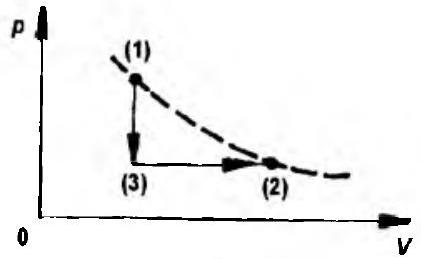
\includegraphics[max width=\textwidth, center]{2025_07_01_5b3ff9fa0d508c8e9f17g-074}

Fig. 2.1 Lucrul mecanic efectuat pentru acest proces este:\\
A) 300 J ;\\
B) 350 J ;\\
C) 400J;\\
D) 375 J ; E) 380 J ; F) 100 J .\\
(Ion M. Popescu)\\
2.6. O masă de oxigen de volum $V_{1}=2 \mathrm{~m}^{3}$ se află la presiunea $p_{1}=2 \cdot 10^{5} \mathrm{~N} / \mathrm{m}^{2}$. Gazul are $C_{V}=5 R / 2$. El este încălzit izobar şi se destinde până la volumul $V_{2}=6 \mathrm{~m}^{3}$, apoi izocor până ce presiunea devine $p_{3}=5 \cdot 10^{5} \mathrm{~N} / \mathrm{m}^{2}$. Variația energiei interne in aceste procese este:\\
A) $6 \cdot 10^{6} \mathrm{~J}$;\\
B) $6,4 \cdot 10^{6} \mathrm{~J}$;\\
C) $6,5 \cdot 10^{5} \mathrm{~J}$;\\
D) $3 \cdot 10^{8} \mathrm{~J}$;\\
E) $10^{7} \mathrm{~J}$; F) $6,5 \cdot 10^{6} \mathrm{~J}$.\\
(Ion M. Popescu)\\
2.7.* Încălzind un gaz cu $\Delta T=100 \mathrm{~K}$, viteza termică a moleculelor creşte de la $v_{T_{1}}=400 \mathrm{~m} / \mathrm{s}$ la $v_{T_{2}}=500 \mathrm{~m} / \mathrm{s}$.

Constanta generală a gazelor fiind $R=8,31 \mathrm{~J} / \mathrm{mol} \cdot \mathrm{K}$ gazul are masa molară:\\
A) $29 \mathrm{~kg} / \mathrm{kmol}$;\\
B) $28 \cdot 10^{-3} \mathrm{~kg} / \mathrm{mol}$;\\
C) $32 \cdot 10^{-3} \mathrm{~kg} / \mathrm{mol}$;\\
D) $30 \mathrm{~kg} / \mathrm{kmol}$;\\
E) $28 \mathrm{~kg} / \mathrm{mol}$;\\
F) $14 \cdot 10^{-3} \mathrm{~kg} / \mathrm{mol}$.\\
(Ion M. Popescu)\\
2.8. În condiții normale de temperatură şi presiune ( $T=273,15 \mathrm{~K}$ şi $p=1 \mathrm{~atm}$ ), numărul lui Avogadro find $N_{A}=6,0234 \cdot 10^{23} \mathrm{molecule} / \mathrm{mol}$ şi volumul molar $V_{\mu_{0}}=22,42 \cdot 10^{-3} \mathrm{~m}^{3} / \mathrm{mol}$, numărul de molecule aflate intr-un volum $V=1 \mathrm{~m}^{3}$ de oxigen saui de azot este:\\
A) $2,7 \cdot 10^{25}$ molecule; $2,5 \cdot 10^{25}$ molecule;\\
B) $2 \cdot 10^{26}$ molecule;\\
C) $2,5 \cdot 10^{25}$ molecule; $2,8 \cdot 10^{25}$ molecule;\\
D) $2,7 \cdot 10^{25}$ molecule;\\
E) $2 \cdot 10^{26}$ molecule; $3 \cdot 10^{25}$ molecule;\\
F) $8 \cdot 10^{32}$ molecule.\\
2.9. Numărul lui Avogadro fiind $N_{A}=6,024 \cdot 10^{23}$ molecule $/ \mathrm{mol}$ şi masa ग-: esulară a oxigenului $\mu_{\mathrm{O}_{2}}=32 \cdot 10^{-3} \mathrm{~kg} / \mathrm{mol}$ într-o masă de 2 kg de oxigen res:ndu-se un număr de molecule egal cu:\\
A) $3,765 \cdot 10^{25}$ molecule;\\
B) $3 \cdot 10^{25}$ molecule;\\
C) $3 \cdot 10^{26}$ molecule ;\\
D) $3,765 \cdot 10^{26}$ molecule ;\\
E) $2,765 \cdot 10^{25}$ molecule;\\
F) $3,8 \cdot 10^{25}$ molecule.\\
(Ion M. Popescu)\\
2.10.* Numărul lui Avogadro este $N_{A}=6,023 \cdot 10^{23}$ molecule $/ \mathrm{mol}$. -esıunea azotului find $p=56 \cdot 10^{3} \mathrm{Nm}^{2}$, viteza termică $v_{T}=600 \mathrm{~m} / \mathrm{s}$ şi masa -ară $\mu=28 \cdot 10^{-3} \mathrm{~kg} / \mathrm{mol}$, concentratia moleculelor acestuia este:\\
A) $10^{24} \mathrm{~m}^{-3}$;\\
B) $5 \cdot 10^{24} \mathrm{~m}^{-3}$;\\
C) $10^{25} \mathrm{~m}^{-3}$;\\
D) $3 \cdot 10^{25} \mathrm{~m}^{-3}$;\\
E) $5 \cdot 10^{32} \mathrm{~m}^{-3}$;\\
F) $2 \cdot 10^{25} \mathrm{~m}^{-3}$\\
(Ion M. Popescu)\\
2.11. Dacă un agregat pentru obținerea vidului ar permite realizarea unei resiumi intr-un vas egală cu $p=10^{-13}$ tori, numărul moleculelor de gaz aflate ==-un volum $V=1 \mathrm{~cm}^{3}$ la presiunea amintită şi temperatura $T=360 \mathrm{~K}$ $\because_{1}=6,023 \cdot 10^{23}$ molecule $/ \mathrm{mol}$ şi $R=8,31 \mathrm{~J} / \mathrm{mol} \cdot \mathrm{K}$ ) ar fi:\\
A) $2,68 \cdot 10^{4}$ molecule ;\\
B) $3 \cdot 10^{4}$ molecule;\\
C) $3,5 \cdot 10^{3}$ molecule ;\\
D) $4 \cdot 10^{4}$ molecule;\\
E) $5,3 \cdot 10^{3}$ molecule;\\
F) $2,68 \cdot 10^{3}$ molecule.\\
(Ion M. Popescu)\\
2.12. Într-o butelie de volum $V=6,25 \mathrm{~m}^{3}$, se păstrează oxigen comprimat la resiunea $p=100 \mathrm{~atm}$ şi temperatura $t=27^{\circ} \mathrm{C}$. În condiții normale de :=mperatură şi presiune ( $T_{0}=273 \mathrm{~K}$ şi $p_{0}=1 \mathrm{~atm}$ ), volumul oxigenului este:\\
A) $560 \mathrm{~m}^{3}$;\\
B) $565 \mathrm{~m}^{3}$;\\
C) $467,25 \mathrm{~m}^{3}$;\\
D) $570 \mathrm{~m}^{3}$;\\
E) $568,75 \mathrm{~m}^{3}$;\\
F) $568 \mathrm{~m}^{3}$.\\
(Ion M. Popescu)\\
2.13. Dioxidul de carbon ( $\mu=44 \cdot 10^{-3} \mathrm{~kg} / \mathrm{mol}$ ), aflat într-un volum $\because=50$ litri la temperatura $t=2^{\circ} \mathrm{C}$ şi presiunea $p=1,66 \cdot 10^{7} \mathrm{~N} / \mathrm{m}^{2}$ are masa $R=8,31 \mathrm{~J} / \mathrm{mol} \cdot \mathrm{K}$ ):\\
A) 16 kg ;\\
B) 13 kg ;\\
C) 15 kg ;\\
D) $15,5 \mathrm{~kg}$;\\
E) 17 kg ;\\
F) 14 kg .\\
2.14. Un gaz aflat în condiţii normale de temperatură și presiune ( $T_{0}$ şi $p_{0}$ ) are densitatea $\rho_{0}$, iar când se schimbă condițiile de temperatură şi presiune devenind $T \neq T_{0}$ şi $p \neq p_{0}$, densitatea gazului este:\\
A) $\frac{p}{p_{0}} \frac{T}{T_{0}} \frac{1}{\rho_{0}}$;\\
B) $\frac{p_{0}}{p} \frac{T_{0}}{T} \rho_{0}$;\\
C) $p p_{0} \frac{T}{T_{0}} \rho_{0}$;\\
D) $p p_{0} T T_{0} \rho_{0}$;\\
E) $\frac{p p_{0}}{T T_{0} \rho_{0}}$;\\
F) $\rho_{0} \frac{p}{p_{0}} \frac{T_{0}}{T}$.\\
(Ion M. Popescu)\\
2.15. Într-un cilindru cu piston se află aer la presiunea atmosferică normală $p_{0}=10^{5} \mathrm{~N} / \mathrm{m}^{2}$, pistonul având masa neglijabilă şi secţiunea $S=250 \mathrm{~cm}^{2}{ }_{\text {t }}$ Inițial, pistonul se află la distanta $d_{1}=1,8 \mathrm{~m}$ de fundul cilindrului și pentru a-1 aduce încet la distanța $d_{2}=1,2 \mathrm{~m}$ se acționează asupra pistonului pentru a ajunge în poziția finală (frecările fiind neglijabile) cu forta:\\
A) 1 kN ;\\
B) $1,25 \mathrm{kN}$;\\
C) $1,5 \mathrm{kN}$;\\
D) 2 kN ;\\
E) $1,3 \mathrm{kN}$;\\
F) 8 kN .\\
(Ion M. Popescu)\\
2.16. Într-un vas de volum $V=0,2075 \mathrm{~m}^{3}$ se află heliu (de masă molară $\mu=4 \cdot 10^{-3} \mathrm{~kg} / \mathrm{mol}$ ) la presiunea $p_{1}=1,2 \cdot 10^{5} \mathrm{~N} / \mathrm{m}^{2}$ şi temperatura $t_{1}=27^{\circ} \mathrm{C}$. Introducând heliu în vas până când presiunea a devenit $p_{2}=2,8 \cdot 10^{5} \mathrm{~N} / \mathrm{m}^{2}$ şi temperatura $t_{2}=47^{\circ} \mathrm{C}$, masa heliului introdus este ( $R=8,3 \mathrm{IJ} / \mathrm{mol} \cdot \mathrm{K}$ ):\\
A) $4,5 \cdot 10^{-2} \mathrm{~kg}$;\\
B) $4,75 \cdot 10^{-2} \mathrm{~kg}$;\\
C) $4,75 \cdot 10^{-3} \mathrm{~kg}$;\\
D) $4,55 \cdot 10^{-2} \mathrm{~kg}$;\\
E) $4 \cdot 10^{-2} \mathrm{~kg}$;\\
F) $5 \cdot 10^{-2} \mathrm{~kg}$.\\
(Ion M. Popescu)\\
2.17. Un vas cilindric orizontal contine un gaz împărțit cu ajutorul unui perete mobil în două părţi, având raportul volumelor $V_{1} / V_{2}=0,8$. Temperatura gazului de volum $V_{1}$ este $t_{1}=167^{\circ} \mathrm{C}$, iar temperatura gazului de volum $V_{2}$ este $t_{2}=255^{\circ} \mathrm{C}$. Presiunea în ambele compartimente este aceeaşi, egalǎ cu $p$. Când cele două parți ale vasului sunt aduse la aceeaşi temperatură, raportul volumelor ocupate de cele două gaze devine:\\
А) 0,9 ;\\
B) 0,94 ;\\
C) 0,98 ;\\
D) 1,2 ;\\
E) 0,96 ;\\
F) 0,38 .\\
2.18. În condiții normale de temperatură şi presiune ( $T_{0}=273 \mathrm{~K}$, $\therefore=101325 \mathrm{~N} / \mathrm{m}^{2}$ ) densitatea gazului este $\rho_{0}=1,293 \mathrm{~kg} / \mathrm{m}^{3}$ şi coeficientul i:abatic $\gamma=1,41$, adică gazul are căldura specifică la presiune constantă $c_{p}$ :\\
A) $900 \mathrm{~J} / \mathrm{kgK}$;\\
B) $980 \mathrm{~J} / \mathrm{kgK}$;\\
C) $800 \mathrm{~J} / \mathrm{kgK}$;\\
D) $987 \mathrm{~J} / \mathrm{kgK}$;\\
E) $1000 \mathrm{~J} / \mathrm{kgK}$;\\
F) $500 \mathrm{~J} / \mathrm{kgK}$.\\
(Ion M. Popescu)\\
2.19. Se cunosc $N_{A}=6,023 \cdot 10^{23}$ molecule $/ \mathrm{mol}$ şi $k_{B}=1,38 \cdot 10^{-23} \mathrm{~J} \cdot \mathrm{~K}^{-1}$. Un ziz cu căldură specificã izobară $c_{p}=5,2 \cdot 10^{3} \mathrm{~J} / \mathrm{kg} \cdot \mathrm{K}$ şi căldura specifică izocoră $\therefore=3,2 \cdot 10^{3} \mathrm{~J} / \mathrm{kg} \cdot \mathrm{K}$, are masa molară:\\
A) $4 \cdot 10^{-3} \mathrm{~kg} \cdot \mathrm{~mol}^{-1}$;\\
B) $4,14 \cdot 10^{-3} \mathrm{~kg} \cdot \mathrm{~mol}^{-1}$;\\
C) $3,92 \cdot 10^{-3} \mathrm{~kg} \cdot \mathrm{~mol}^{-1}$;\\
D) $4,2 \cdot 10^{-3} \mathrm{~kg} \cdot \mathrm{~mol}^{-1}$;\\
E) $5 \cdot 10^{-3} \mathrm{~kg} \cdot \mathrm{~mol}^{-1}$;\\
F) $4,3 \cdot 10^{-3} \mathrm{~kg} \cdot \mathrm{~mol}^{-1}$.\\
(Ion M. Popescu)\\
2.20. O cantitate de oxigen ( $C_{V}=5 R / 2$ ) ocupă volumul $V_{1}=1,2 \mathrm{~m}^{3}$ la Tesiunea $p_{1}=2,5 \cdot 10^{5} \mathrm{~N} / \mathrm{m}^{2}$. Gazul este încălzit izobar şi se destinde până la ¿ Jumul $V_{2}=3,2 \mathrm{~m}^{3}$, apoi izocor până la presiunea $p_{3}=5,25 \cdot 10^{5} \mathrm{~N} / \mathrm{m}^{2}$ şi în heste procese variația energiei interne a gazului este:\\
A) $3,45 \mathrm{MJ}$;\\
B) 3 MJ ;\\
C) 10 kJ ;\\
D) $3,45 \mathrm{~kJ}$;\\
E) $3,5 \mathrm{MJ}$;\\
F) $3,8 \mathrm{~kJ}$.\\
(Ion M. Popescu)\\
2.21. Un gaz care participă la o transformare ciclică al cărei randament este - $=0,1$, efectuează lucrul mecanic $L=400 \mathrm{~J}$. În decursul acestui ciclu, căldura : :Jată de gaz la sursa rece este:\\
A) 3000 J ;\\
B) 4000 J ;\\
C) -3600 J ;\\
D) 5000 J ;\\
E) 6000 J ; F)\\
-2000J.\\
(Ion M. Popescu)\\
2.22. Un gaz se află în condiții normale de temperatură şi presiune dacă:\\
A) $t=0^{\circ} \mathrm{C}$ şi $p=\mathrm{latm}$;\\
B) $t=20^{\circ} \mathrm{C}$ şi $p=1 \mathrm{~atm}$;\\
C) $t=0^{\circ} \mathrm{C}$ şi $p=10^{6} \mathrm{~N} / \mathrm{m}^{2}$;\\
D) $t=273^{\circ} \mathrm{C}$ şi $p=10^{5} \mathrm{~N} / \mathrm{m}^{2}$;\\
E) $T=0 \mathrm{~K}$ şi $p=$ latm;\\
F) $T=0 \mathrm{~K}$ şi $p=1,013 \cdot 10^{5} \mathrm{~N} / \mathrm{m}^{2}$.\\
2.23. Numărul de molecule dintr-un mol de substanță este:\\
A) $6,023 \cdot 10^{26}$;\\
B) $6,023 \cdot 10^{23}$;\\
C) $6,023 \cdot 10^{-26}$;\\
D) $6,023 \cdot 10^{-23}$;\\
E) $6,023 \cdot 10^{25}$;\\
F) $6,023 \cdot 10^{22}$.\\
(Alexandru M. Preda)\\
2.24. Legea formulată astfel "volume egale de gaze diferite, aflate în aceleaşi condiții de temperatură și presiune, au acelaşi număr de molecule", reprezintă:\\
A) Legea lui Dalton;\\
B) Legea proporțiilor definite;\\
C) Legea lui Brown;\\
D) Legea lui Avogadro;\\
E) Legea proporțiilor multiple;\\
F) Legea volumelor a lui Gay-Lussac.\\
(Alexandru M. Preda)\\
2.25. Un mol de substanţă se defineşte astfel:\\
A) cantitatea de substanță a cărei densitate este numeric egală cu masa moleculară a substanței date;\\
B) cantitatea de substantăa a cărei masă molară este egală cu a 12-a parte din masa atomică a izotopului de carbon $\left({ }_{6}^{12} \mathrm{C}\right)$;\\
C) cantitatea de substanță a cărei masă, exprimată în grame, este numeric egală cu masa moleculară relativă a substanței date;\\
D) cantitatea de substantă a cărei masă exprimată în kilograme este numeric egală cu masa moleculară a substanței date;\\
E) cantitatea de substanță care conține $6,023 \cdot 10^{26}$ molecule;\\
F) cantitatea de substanță aflată în condiții normale de temperatură şi presiune.\\
(Alexandru M. Preda)\\
2.26. Să se calculeze numărul de molecule dintr-un kilogram de apă dacă masa moleculară relativă a apei este $\mu=18$ şi numărul lui Avogadro este $N_{A}=$ $=6,023 \cdot 10^{23} \mathrm{molecule} / \mathrm{mol}$ :\\
А) $10^{20}$;\\
В) $3 \cdot 10^{26}$;\\
C) $3 \cdot 10^{20}$;\\
D) $3,301 \cdot 10^{21}$;\\
E) $3,346 \cdot 10^{25}$;\\
F) $10^{23}$.\\
(Alexandru M. Preda)\\
2.27. Energia internă a gazului ideal este o funcție de forma:\\
A) $U=U(t, p)$;\\
В) $U=U(p / V)$;\\
C) $U=U_{0}=$ const.\\
D) $U=U(p, T)$;\\
Е) $U=U(V, T)$;\\
F) $U=U(T)$.\\
2.28. Pentru un mol de gaz ideal monoatomic energia internă va fi:\\
A) $U=\frac{2}{3} R T$;\\
B) $U=\frac{3}{2} R T$;\\
C) $U=\frac{3}{2} k T$;\\
D) $U=\frac{3 R}{\mu} T$;\\
E) $U=\frac{5}{2} R T$;\\
F) $U=k n T$.\\
(Alexandru M. Preda)\\
2.29. Într-un tub de televizor se gǎsesc urme de aer care la temperatura de $\therefore-\mathrm{K}$ are o presiune de $10^{-4} \mathrm{~N} / \mathrm{m}^{2}$. Constanta lui Boltzmann $k=1,38 \cdot 10^{-23} \mathrm{~J} / \mathrm{K}$. -:ncentratia moleculelor din tubul de televizor este:\\
A) $0,44 \mathrm{~m}^{-3}$;\\
B) $1,38 \cdot 10^{-21} \mathrm{~m}^{-3}$;\\
C) $2,26 \cdot 10^{16} \mathrm{~m}^{-3}$;\\
D) $10^{23} \mathrm{~m}^{-3}$;\\
E) $6,023 \cdot 10^{23} \mathrm{~m}^{-3}$;\\
F) $4,46 \cdot 10^{9} \mathrm{~m}^{-3}$.\\
(Alexandru M. Preda)\\
2.30. Un mol de gaz ideal aflat în condiţii normale de temperatură şi presiune capã un volum de $22,42 \mathrm{~m}^{3} / \mathrm{kmol}$. Care este valoarea constantei universale a zelor, exprimată în $\mathrm{J} / \mathrm{mol} \cdot \mathrm{K}$ ?\\
A) $8,31 \cdot 10^{3}$;\\
B) 0,0831 ;\\
C) 8,22 ;\\
D) 8,31 ;\\
E) 831,4 ;\\
F) 8341 .\\
(Alexandru M. Preda)\\
2.31. Capacitatea calorică şi căldura specifică ale unui corp solid sunt date de everesiile:\\
A) $C=\frac{U-p V}{m \Delta T}, c=\frac{Q}{\Delta T}$;\\
В) $C=Q \Delta T, c=m Q \Delta T$;\\
C) $C=\frac{v Q}{\Delta T}, c=\frac{v Q}{m \Delta T}$;\\
D) $C=\frac{p V}{\Delta T}, c=\frac{Q}{\Delta T}$;\\
Е) $C=\frac{U}{\Delta T}, c=\frac{v U}{m \Delta T}$;\\
F) $C=\frac{Q}{\Delta T}, c=\frac{Q}{m \Delta T}$.\\
(Alexandru M. Preda)\\
2.32. Să se afle căldurile molare $C_{V}$ şi $C_{p}$ ale unui gaz perfect dacă $\gamma=1,41$ $\therefore R=8,31 \mathrm{~J} / \mathrm{mol} \cdot \mathrm{K}$.\\
A) $32,58 \mathrm{~J} / \mathrm{mol} \cdot \mathrm{K} 40,89 \mathrm{~J} / \mathrm{mol} \cdot \mathrm{K}$;\\
B) $10,27 \mathrm{~J} / \mathrm{mol} \cdot \mathrm{K} \quad 18,58 \mathrm{~J} / \mathrm{mol} \cdot \mathrm{K}$;\\
C) $20,27 \mathrm{~J} / \mathrm{mol} \cdot \mathrm{K} \quad 28,58 \mathrm{~J} / \mathrm{mol} \cdot \mathrm{K}$;\\
D) $8,31 \mathrm{~J} / \mathrm{mol} \cdot \mathrm{K} \quad 16,62 \mathrm{~J} / \mathrm{mol} \cdot \mathrm{K}$;\\
E) $70,10 \mathrm{~J} / \mathrm{mol} \cdot \mathrm{K} \quad 78,41 \mathrm{~J} / \mathrm{mol} \cdot \mathrm{K}$;\\
F) $22,42 \mathrm{~J} / \mathrm{mol} \cdot \mathrm{K} \quad 8,14 \mathrm{~J} / \mathrm{mol} \cdot \mathrm{K}$.\\
2.33. Lucrul mecanic efectuat de un mol de gaz ideal într-o transformare izotermă de la starea inițială $\left(V_{1}, p_{1}\right)$ la starea finală $\left(V_{2}, p_{2}\right)$ este dat de expresia:\\
A) $L=\left(V_{2}-V_{1}\right)\left(p_{2}-p_{1}\right)$; B) $L=0$; C) $L=C_{p}\left(V_{2}-V_{1}\right)$;\\
D) $L=2,3 R T \lg \frac{p_{2}}{p_{1}}$; E) $\left.L=2,3 R T \lg \frac{V_{2}}{V_{1}} ; \mathrm{F}\right) L=R T \ln \frac{V_{2} p_{2}}{V_{1} p_{1}}$.\\
(Alexandru M. Preda)\\
2.34. Să se calculeze canritatea de căldură absorbită de o cantitate de apă cu masa $m=2 \mathrm{~kg}$ pentru a trece de la temperatura $t_{1}=20^{\circ} \mathrm{C}$ la $t_{2}=80^{\circ} \mathrm{C}$. Se dã: $c=4200 \mathrm{~J} / \mathrm{kg} \cdot \mathrm{K}$.\\
A) 504 kJ ;\\
B) 504 J ;\\
C) 120 J ;\\
D) 252 kJ ;\\
E) 8400 J ;\\
F) 672 kJ .\\
(Alexandru M. Preda)\\
2.35. Ce căldură se degajă la răcirea cu $10^{\circ} \mathrm{C}$ a unui calorifer cu masa de 10 kg şi căldura specifică $500 \mathrm{~J} / \mathrm{kg} \cdot \mathrm{K}$ ?\\
A) 5000 J ;\\
B) $5 \cdot 10^{-3} \mathrm{~J}$;\\
C) 5 J ;\\
D) $5 \cdot 10^{4} \mathrm{~J}$;\\
E) 500 J ;\\
F) $10^{4} \mathrm{~J}$.\\
(Alexandru M. Preda)\\
2.36. Să se afle densitatea aerului dintr-o cameră în care presiunea $p=1 \mathrm{~atm}$ şi temperatura $t=27^{\circ} \mathrm{C}$. Se consideră: masa molară a aerului $\mu=29 \cdot 10^{-3} \mathrm{~kg} / \mathrm{mol}$ şi $R=8,31 \mathrm{~J} / \mathrm{K} \cdot \mathrm{mol}$.\\
A) $10 \mathrm{~kg} / \mathrm{m}^{3}$;\\
B) $1001,18 \mathrm{~kg} / \mathrm{m}^{3}$;\\
C) $1,18 \mathrm{~kg} / \mathrm{m}^{3}$;\\
D) $0,01 \mathrm{~kg} / \mathrm{m}^{3}$;\\
E) $1,1 \cdot 10^{-3} \mathrm{~kg} / \mathrm{m}^{3}$;\\
F) $29 \mathrm{~kg} / \mathrm{m}^{3}$.\\
(Alexandru M. Preda)\\
2.37. Un gaz aflat inițial la temperatura de $0^{\circ} \mathrm{C}$ este încălzit sub presiune constantă până când volumul său se dublează. La ce temperatură a ajuns gazul în urma acestui proces?\\
A) $100^{\circ} \mathrm{C}$;\\
B) $273^{\circ} \mathrm{C}$;\\
C) 273 K ;\\
D) 2730 K ;\\
E) 819 K ;\\
F) 5460 K .\\
(Alexandru M. Preda)\\
2.38. Prin sistemul de răcire al unui compresor se scurge într-o oră un volum de $1,8 \mathrm{~m}^{3}$ de apă care se încălzeşte în compresor cu $6^{\circ} \mathrm{C}$. Care este puterea consumată de motor şi utilizată pentru funcționarea compresorului dacã\\
-andamentul acestuia din urmă este $60 \%$ ?Se consideră:căldura specifică a apei $\therefore=4200 \mathrm{~J} / \mathrm{kgK}$ şi densitatea apei $\rho=1000 \mathrm{~kg} / \mathrm{m}^{3}$ .\\
A) $45,2 \mathrm{~kW}$ ;\\
B) 100 kW ;\\
C) $25,5 \mathrm{~kW}$ ;\\
D) $10,5 \mathrm{~kW}$ ;\\
E) $31,5 \mathrm{~kW}$ ;\\
F) 40 kW .\\
(Alexandru M.Preda)

2.39.Un motor termic funcţionează după ciclul Otto format din două izocore :-3 şi 4-1 şi două adiabate $1-2$ şi 3-4.Să se afle randamentul motorului こョcă $\varepsilon^{\gamma-1}=3$ ,unde $\varepsilon$ este raportul de compresie $V_{1} / V_{2}$ al substanței de lucru,iar este exponentul adiabatic.\\
А) 0,33 ;\\
B)0,66 ;\\
C) 0,50 ;\\
D) 0,25 ;\\
E) 0,55 ;\\
F) 0,77 .\\
(Alexandru M.Preda)\\
2.40.Ciclul Diesel reprezentat în Fig. 2.2 are ca substanțã de lucru un gaz zentru care $\gamma=C_{p} / C_{V}=1,40$ .1-2 şi 3-4 transformări adiabate.Dacă se こonsideră raportul de compresie adiabaticá $n=V_{1} / V_{2}=10$ şi raportul de éstindere preliminară $k=V_{3} / V_{2}=2$ ,să se afle randamentul ciclului,ştiind că $\therefore^{\therefore 4}=2,64$ şi $10^{0,4}=2,51$ .\\
A) 0,64 ;\\
B) 0,46 ;\\
C) 0,33 ;\\
D)0,54 ;\\
E) 0,73 ;F) 0,40 .\\
(Alexandru M.Preda)\\
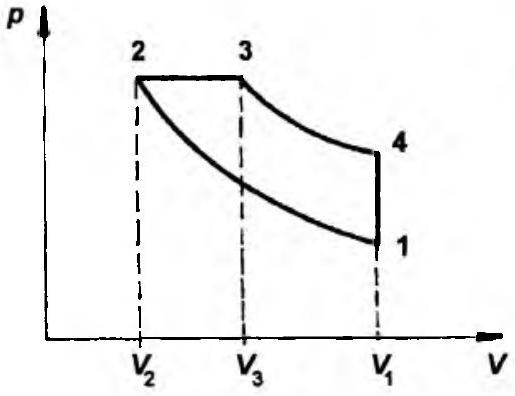
\includegraphics[max width=\textwidth, center]{2025_07_01_5b3ff9fa0d508c8e9f17g-081}

Fig. 2.2\\
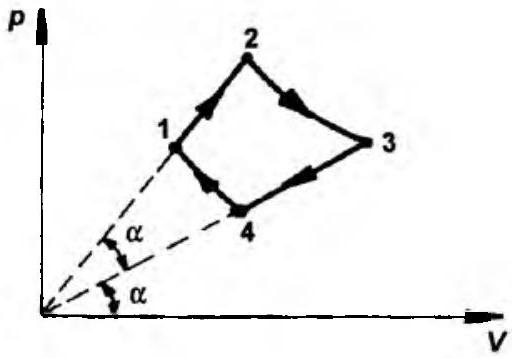
\includegraphics[max width=\textwidth, center]{2025_07_01_5b3ff9fa0d508c8e9f17g-081(1)}

Fig. 2.3

2.41.Un gaz ideal se află la temperatura de 300 K şi are energia cinetică medie a tuturor particulelor sale egală cu $6,2 \mathrm{~J}$ .Dacă constanta lui Boltzmann $\AA=1,38 \cdot 10^{-23} \mathrm{~J} / \mathrm{K}$ să se afle numărul total de particule care formează acest gaz deal.\\
A) $10^{21}$ ;\\
B) $10^{23}$ ;\\
C) $5 \cdot 10^{20}$ ;\\
D) $6 \cdot 10^{23}$ ;\\
E) $10^{26}$ ;\\
F) $10^{18}$ .\\
2.42. O maşină termică functionează cu v moli de gaz perfect după ciclul din Fig. 2.3. Transformările $2-3$ şi $4-1$ sunt izoterme cu temperaturile $T_{2}=500 \mathrm{~K}$ şi respectiv $T_{1}=300 \mathrm{~K}$. Dacă transformările rectilinii 1-2 şi 3-4 au căldurile molare egale cu $2 R$ şi unghiul $\alpha=30^{\circ}$, să se afle randamentul ciclului. Se consideră: $\ln 3=1$.\\
A) 0,30 ;\\
B) 0,15 ;\\
C) 0,66 ;\\
D) 0,33 ;\\
E) 0,50 ;\\
F) 0,20 .\\
(Alexandru M. Preda)\\
2.43. Într-un cilindru orizontal închis la\\
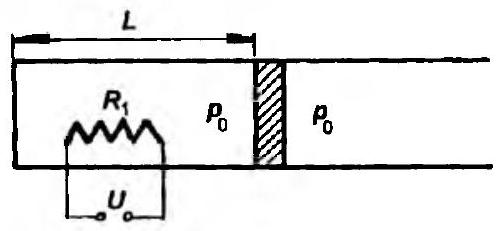
\includegraphics[max width=\textwidth, center]{2025_07_01_5b3ff9fa0d508c8e9f17g-082}

Fig. 2.4 un capăt se află un piston mobil și o rezistență $R_{1}$, de volum neglijabil, conectată la o sursă exterioară de tensiune $U=10 \mathrm{~V}$ şi rezistență internă neglijabilă (Fig. 2.4). În compartimentul închis de lungime $L$ în poziția inițială de echilibru la temperatura $T_{0}=300 \mathrm{~K}$ se află $v=4 / R$ moli de gaz perfect monoatomic. Să se determine valoarea rezistenței $R_{1}$ astfel ca după timpul $\tau=60 \mathrm{~s}$ de la conectarea sursei la rezistența $R_{1}$ noua poziție de echilibru a pistonului mobil să fie la $L_{1}=1,25 L$. Se presupune că întreaga căldură degajată de rezistența $R_{1}$ este absorbitã de gazul din compartimentul închis.\\
A) $4 \Omega$;\\
B) $40 \Omega$;\\
C) $0,25 \Omega$;\\
D) $8 \Omega$;\\
E) $25 \Omega$;\\
F) $100 \Omega$.\\
(Alexandru M. Preda)\\
2.44. Sub acțiunea unei forțe orizontale un corp care are căldura specifică $c=100 \mathrm{~J} / \mathrm{kg} \cdot \mathrm{grad}$ se deplasează uniform pe un plan orizontal având coeficientul de frecare $\mu=0,5$. Dacă se presupune că numai jumătate din căldura degajată prin frecare este absorbită de corp să se afle cu cât creşte temperatura lui după ce a parcurs distanta $s=80 \mathrm{~m}\left(g=10 \mathrm{~m} / \mathrm{s}^{2}\right)$.\\
A) 4 grade ;\\
B) 0,4 grade ;\\
C) 1 grad;\\
D) 2 grade ;\\
E) 0,5 grade ;\\
F) 8 grade .\\
(Alexandru M. Preda)\\
2.45. Un gaz ideal al cărui exponent adiabatic este $\gamma$ suferă o dilatare descrisă de ecuația $p=b V$ unde $b>0$ este o constantă. În cursul dilatării presiunea creşte de la $p_{1}$ la $p_{2}=n p_{1}$. Variația energiei interne a gazului în acest proces este:\\
A) $(\gamma+1) b n V_{1}^{2}$;\\
B) $(\gamma-1) n^{2} b V_{1}^{2}$;\\
C) $\frac{n^{2} b V_{1}^{2}}{\gamma-1}$;\\
D) $\frac{\left(n^{2}-1\right) b V_{1}^{2}}{\gamma-1}$;\\
E) $\gamma b\left(n^{2}-1\right) V_{1}^{2}$;\\
F) $\frac{\left(n^{2}+1\right) b V_{1}^{2}}{\gamma+1}$.\\
(Constantin P. Cristescu)\\
2.46. Raportul dintre presiunea şi densitatea unui gaz ideal este constant în -Esiormarea:\\
A) izobară; B) în orice transformare; C) izotermă;\\
D) în nici o transformare; E) adiabaticǎ; F) izocoră.\\
(Constantin P. Cristescu)\\
2.47. Într-un calorimetru cu capacitate calorică neglijabilă se amestecă mase Ele din acelaşi lichid aflate la temperaturile $t_{1}=30^{\circ} \mathrm{C}, t_{2}=6^{\circ} \mathrm{C}$ şi $t_{3}=87^{\circ} \mathrm{C}$. - emperatura amestecului este:\\
A) $32^{\circ} \mathrm{C}$;\\
B) $55^{\circ} \mathrm{C}$;\\
C) $35^{\circ} \mathrm{C}$;\\
D) $47^{\circ} \mathrm{C}$;\\
E) $38^{\circ} \mathrm{C}$;\\
F) $41^{\circ} \mathrm{C}$.\\
(Constantin P. Cristescu)\\
2.48. Un mol de gaz ideal aflat la temperatura $t_{1}=37^{\circ} \mathrm{C}$ suferă o transformare こっbară în care efectuează lucrul mecanic $L=1662 \mathrm{~J}$.

Cunoscând $R=8,31 \mathrm{~J} / \mathrm{mol} \cdot \mathrm{K}$ temperatura gazului în starea finală este:\\
A) 510 K ;\\
B) 470 K ;\\
C) 544 K ;\\
D) 483 K ;\\
E) $220^{\circ} \mathrm{C}$;\\
F) $183^{\circ} \mathrm{C}$.\\
(Constantin P. Cristescu)\\
2.49. O maşină termică ideală funcționează după un ciclu Carnot între anperaturile $t_{1}=227^{\circ} \mathrm{C}$ şi $t_{2}=27^{\circ} \mathrm{C}$ producând în cursul unui ciclu un lucru -ecanic $L=8 \cdot 10^{4} \mathrm{~J}$. Căldura cedată sursei reci într-un ciclu este:\\
A) $3 \cdot 10^{5} \mathrm{~J}$;\\
B) $1,2 \cdot 10^{5} \mathrm{~J}$;\\
C) $1,8 \cdot 10^{5} \mathrm{~J}$;\\
D) $3,6 \cdot 10^{5} \mathrm{~J}$;\\
E) $2,8 \cdot 10^{5} \mathrm{~J}$;\\
F) $4,2 \cdot 10^{5} \mathrm{~J}$.\\
(Constantin P. Cristescu)\\
2.50.* Un gaz ideal suferă o transformare generală în care presiunea se sublează iar densitatea se înjumătățeşte. Viteza termică a moleculelor se modifică sitfel:\\
A) se înjumătățeşte;\\
B) se dublează;\\
C) creşte de $\sqrt{2}$ ori;\\
D) scade de $\sqrt{2}$ ori;\\
E) scade de 4 ori;\\
F) rămâne nemodificată.\\
2.51.* Într-o incintǎ se află oxigen ( $\mu=32 \cdot 10^{-3} \mathrm{~kg} / \mathrm{mol}$ ) la presiunea $p=8 \cdot 10^{4} \mathrm{~N} / \mathrm{m}^{2}$, viteza termică a moleculelor find $v_{T}=500 \mathrm{~m} / \mathrm{s}$.

Considerând numǎrul lui Avogadro $N_{A}=6 \cdot 10^{23} \mathrm{molec} / \mathrm{mol}$ concentrația $n$ a moleculelor din vas este:\\
A) $10^{24} \mathrm{molec} / \mathrm{m}^{3}$;\\
B) $2,5 \cdot 10^{24} \mathrm{molec} / \mathrm{m}^{3}$;\\
C) $2,7 \cdot 10^{25} \mathrm{molec} / \mathrm{m}^{3}$;\\
D) $3 \cdot 10^{25} \mathrm{molec} / \mathrm{m}^{3}$;\\
E) $1,8 \cdot 10^{25} \mathrm{molec} / \mathrm{m}^{3}$;\\
F) $5,3 \cdot 10^{24} \mathrm{molec} / \mathrm{m}^{3}$.\\
(Constantin P. Cristescu)\\
2.52. Randamentul unei maşini termice care ar funcționa după un ciclu Carnot între două surse ale căror temperaturi coincid cu temperaturile maximă şi minimă atinse în ciclul desenat în Fig. 2.5 este:\\
A) $\frac{1}{3}$;\\
B) $\frac{2}{3}$;\\
C) $\frac{5}{6}$,\\
D) $\frac{1}{6}$;\\
E) $\frac{4}{5}$;\\
F) nu poate fi calculat din datele furnizate.\\
(Constantin P. Cristescu)\\
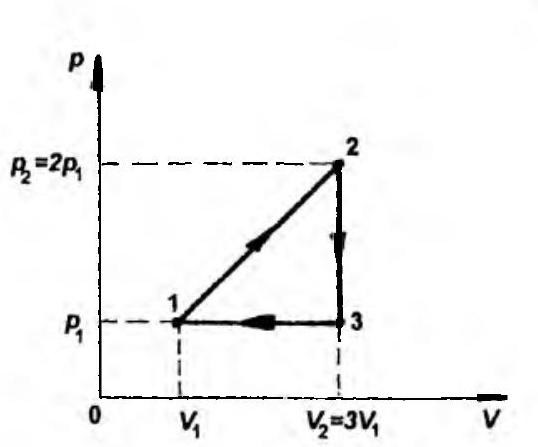
\includegraphics[max width=\textwidth, center]{2025_07_01_5b3ff9fa0d508c8e9f17g-084}\\
2.53. Un gaz ideal monoatomic având volumul $V_{1}$ la presiunea $p_{1}$ este comprimat izobar până la volumul $V_{2}=\frac{V_{1}}{n}$ şi apoi încălzit izocor până la presiunea $p_{2}=\frac{n}{2} p_{1}$. Dacă în starea inițială energia internă este $U_{1}$, energia $U_{2}$ în starea finală este:\\
A) $2 U_{1}$;\\
B) $U_{1}$;\\
C) $\left(\frac{n}{2}+1\right) U_{1}$;\\
D) $\frac{n}{2} U_{1}$;\\
E) $\frac{2 U_{1}}{n}$;\\
F) $\frac{U_{1}}{2}$.\\
2.54. Se consideră transformările unei mase de gaz ideal reprezentate grafic în Zégura 2.6. Dacă între pantele lor există relația $\operatorname{tg} \alpha_{1}=\frac{1}{2} \operatorname{tg} \alpha_{2}=\frac{1}{3} \operatorname{tg} \alpha_{3}$ care s.ntre următoarele afirmații este eronată ?\\
A) transformările sunt izobare; B) $p_{2}=\frac{p_{1}+p_{3}}{2}$;\\
C) pentru curba 3 presiunea este cea mai mică;\\
D) pentru curba 1 presiunea este cea mai mare;\\
E) $p_{2}=\frac{p_{1}}{2}$; F) $\frac{p_{3}}{p_{2}}=\frac{2}{3}$.\\
(Constantin P. Cristescu)\\
2.55. Un tub de lungime $L$ închis la un capăt se scufundǎ vertical cu capătul Leschis în jos intr-un lichid cu densitatea $\rho=10^{3} \mathrm{~kg} / \mathrm{m}^{3}$, porțiunea scufundată suand lungimea $l=66 \mathrm{~cm}$. Lungimea coloanei de lichid din tub este $l^{\prime}=6 \mathrm{~cm}$. Considerând $g=10 \mathrm{~m} / \mathrm{s}^{2}$ şi ştiind că presiunea atmosferică $p_{0}=10^{5} \mathrm{~N} / \mathrm{m}^{2}$, -ngimea $L$ a tubului este:\\
A) 106 cm ;\\
B) 100 cm ;\\
C) $98,8 \mathrm{~cm}$;\\
D) 95 cm ;\\
E) 110 cm ;\\
F) 101 cm .\\
(Constantin P. Cristescu)\\
2.56. Deschizând un vas, presiunea gazului scade cu $f_{1}=28 \%$, iar :emperatura absolută cu $f_{2}=10 \%$. Cu cât la sută scade masa gazului ?\\
A) $33,3 \%$;\\
B) $30 \%$;\\
C) $20 \%$;\\
D) $25 \%$;\\
E) $21 \%$;\\
F) $40 \%$.\\
2.57. Randamentul ciclului din Fig. 2.7 este (se cunoaşte coeficientul adiabatic $\because$ al gazului care execută ciclul):\\
A) $\eta=\frac{\gamma-1}{\gamma+1}$;\\
B) $\eta=\frac{3}{2} \frac{\gamma-1}{6 \gamma+1}$;\\
C) $\eta=\frac{\gamma-1}{6 \gamma-1}$;\\
D) $\eta=\frac{2(\gamma-1)}{\gamma+1}$;\\
Е) $\eta=\frac{3(\gamma-1)}{6 \gamma+1}$;\\
F) $\eta=\frac{3 \gamma}{6 \gamma+1}$.\\
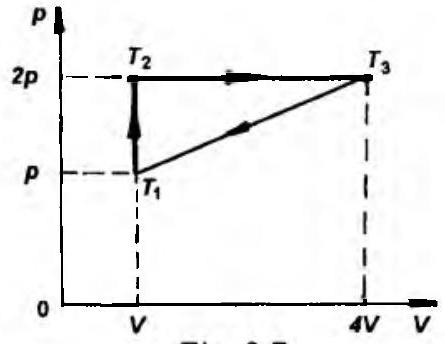
\includegraphics[max width=\textwidth, center]{2025_07_01_5b3ff9fa0d508c8e9f17g-085}

Fig. 2.7\\
2.58. Un vas cilindric cu secțiunea de $10 \mathrm{~cm}^{2}$ şi masa de 200 g , aşezat pe un plan orizontal cu gura în jos, închide aer la temperatura de $27^{\circ} \mathrm{C}$ şi presiunea atmosferică normală de $10^{5} \mathrm{~N} / \mathrm{m}^{2}$. Găsiți concentrația moleculelor din vasul cilindric şi temperatura la care aerul începe să iasă din vas. Se cunoaşte $k=1,38 \cdot 10^{-23} \mathrm{~J} / \mathrm{K}$.\\
A) $n=24 \cdot 10^{25} \mathrm{~m}^{-3} ; T_{2}=35^{\circ} \mathrm{C}$;\\
B) $n=12 \cdot 10^{24} \mathrm{~m}^{-3} ; T_{2}=300 \mathrm{~K}$;\\
C) $n=2,4 \cdot 10^{25} \mathrm{~m}^{-3} ; T_{2}=306 \mathrm{~K}$;\\
D) $n=2,4 \cdot 10^{25} \mathrm{~m}^{-3} ; T_{2}=275 \mathrm{~K}$;\\
E) $n=20 \cdot 10^{24} \mathrm{~m}^{-3} ; T_{2}=288 \mathrm{~K}$;\\
F) $n=2,4 \cdot 10^{25} \mathrm{~m}^{-3} ; T_{2}=316 \mathrm{~K}$.

\section*{(Maria Honciuc)}
2.59. Un motor termic funcționează după un ciclu Carnot cu randamentul de $40 \%$. Temperatura sursei reci este de $27^{\circ} \mathrm{C}$, iar maşina primeşte de la sursa caldă cantitatea de căldură de 60 kJ în fiecare secundă. Să se găsească cu câte grade ar trebui coborâtă temperatura sursei reci astfel încât randamentul motorului să crească la $50 \%$ şi care este puterea inițială a motorului:\\
A) $50^{\circ} \mathrm{C} ; 2,4 \mathrm{~kW}$; B) 50 K ; 24 kW ; C) $20^{\circ} \mathrm{C} ; 12 \mathrm{~kW}$;\\
D) 20 K ; 24 kW ; E) 50 K ; 25 kW ; F) 50 K ; 60 kW .\\
(Maria Honciuc)\\
2.60. Un gaz ideal diatomic disociază în proporție de $f$ procente din moleculele sale. Căldura molară izocoră a gazului format este:\\
(Se cunosc $C_{V_{1}}=\frac{3}{2} R ; C_{V_{2}}=\frac{5}{2} R ; f=0,5$ ).\\
A) $C=\frac{5}{6} R$;\\
B) $C=\frac{15}{6} R$;\\
C) $C=\frac{6}{11} R$;\\
D) $C=\frac{11}{6} R$;\\
E) $C=\frac{5}{2} R$;\\
F) $C=2 R$.\\
2.61. Formula fundamentală a teoriei cinetico-moleculare este:\\
A) $p=\frac{2}{3} N \frac{\bar{v}^{2}}{2}$;\\
B) $p=\frac{1}{3} N m \bar{v}^{2}$;\\
C) $p=\frac{2}{3} \frac{N}{V} \frac{m \bar{v}^{2}}{2}$;\\
D) $p=N k T$;\\
E) $p=\frac{2}{3} N \bar{\varepsilon}$;\\
F) $p=\frac{2}{3} N \frac{m \bar{v}^{2}}{3}$.\\
2.62.* Un gaz ideal $(\gamma=7 / 5)$ se destinde adiabatic de la $V_{1}$ la $V_{2}=32 V_{1}$. Raportul vitezelor termice ale moleculelor este:\\
A) $3 / 2$;\\
B) 4 ;\\
C) 2,4 ;\\
D) 0,5 ;\\
E) 2 F) 4,2 .\\
(Corneliu Ghizdeanu)\\
2.63. Căldura schimbatã în procesul $1-2$ din F.g. 2.8 este:\\
А) 0 ; В) $n p_{0} V_{0} \ln (1 / n)$;\\
C) $(1 / 2) p_{0} V_{0}\left(n^{2}-1\right)$;\\
D) $n p_{0} V_{0} \ln (n)$;\\
Е) $\frac{p_{0} V_{0}}{2}\left(1-n^{2}\right)$;\\
F) $\frac{p_{0} V_{0}}{2}\left(1-2 n^{2}\right)$.\\
(Corneliu Ghizdeanu)\\
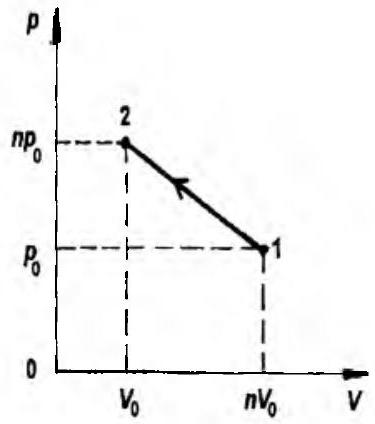
\includegraphics[max width=\textwidth, center]{2025_07_01_5b3ff9fa0d508c8e9f17g-087}

Fig. 2.8\\
2.64.* Viteza termică a unei mici picături de ază $r$ şi de densitate $\rho$ aflată în aer la temperatura $T$ este:\\
A) $\frac{3}{2} \sqrt{k T /\left(\pi \rho r^{3}\right)}$;\\
В) $\frac{3}{2} \sqrt{k} \bar{T} / \pi \rho r^{3}$;\\
C) $\frac{1}{2} \sqrt{k T /\left(\pi \rho r^{3}\right)}$;\\
D) $\sqrt{3 k T / \mu}$;\\
E) $\sqrt{3 R T / m}$;\\
F) $\frac{3}{2} \sqrt{k T /\left(\pi \rho^{2} r^{3}\right)}$.\\
(Corneliu Ghizdeanu)\\
2.65.* Două vase $V_{1}$ şi $V_{2}$ legate printr-un tub de volum neglijabil conțin același gaz la presiunea $p$ şi temperatura $T_{1}$. Vasul $V_{1}$ se încălzeşte la $o$ :emperatură $T_{1}^{\prime}=n T_{1}$, iar vasul $V_{2}$ rămâne la temperatura $T_{1}$. Variația relativă a itezei termice a moleculelor din vasul $V_{1}$ este:\\
A) $\sqrt{n}$;\\
B) $1-\sqrt{n}$;\\
C) $\sqrt{n}-1$;\\
D) $\frac{\sqrt{n}}{n}$;\\
E) $n^{2}$;\\
F) $-\frac{\sqrt{n}}{n}$.\\
(Corneliu Ghizdeanu)\\
2.66. O masă de gaz se află închisă într-un vas la presiunea $p_{0}$ şi volumul $V_{0}$. Dacã presiunea gazului este schimbată izoterm cu $2 \cdot 10^{5} \mathrm{~N} / \mathrm{m}^{2}$ volumul acestuia se schimbă cu $3 \cdot 10^{-3} \mathrm{~m}^{3}$, iar la o schimbare izotermă cu $5 \cdot 10^{5} \mathrm{~N} / \mathrm{m}^{2}$ a presiunii, volumul se modifică cu $5 \cdot 10^{-3} \mathrm{~m}^{3}$. Care sunt valorile inițiale ale presiunii şi volumului gazului ?\\
A) $p_{0}=10^{5} \frac{\mathrm{~N}}{\mathrm{~m}^{2}} ; V_{0}=5 \cdot 10^{-3} \mathrm{~m}^{3} ;$ B) $p_{0}=4 \cdot 10^{5} \frac{\mathrm{~N}}{\mathrm{~m}^{2}} ; V_{0}=9 \cdot 10^{-3} \mathrm{~m}^{3}$;\\
C) $p_{0}=9 \cdot 10^{5} \frac{\mathrm{~N}}{\mathrm{~m}^{2}} ; V_{0}=10^{-2} \mathrm{~m}^{3} ;$ D) $p_{0}=10^{5} \frac{\mathrm{~N}}{\mathrm{~m}^{2}} ; V_{0}=10^{-2} \mathrm{~m}^{3} ;$\\
E) $p_{0}=3 \cdot 10^{5} \frac{\mathrm{~N}}{\mathrm{~m}^{2}} ; V_{0}=2 \cdot 10^{-1} \mathrm{~m}^{3} ;$ F) $p_{0}=4 \cdot 10^{4} \frac{\mathrm{~N}}{\mathrm{~m}^{2}} ; V_{0}=9 \cdot 10^{-1} \mathrm{~m}^{3}$.\\
(Marcel Dobre)\\
2.67.* Ce temperatură corespunde unei viteze termice a moleculelor de gaz egală cu viteza unui avion supersonic $v=700 \mathrm{~m} / \mathrm{s}$. Se cunosc: $\mu=29 \mathrm{~kg} / \mathrm{kmol}$, $R=8314 \mathrm{~J} / \mathrm{kmol} \cdot \mathrm{K}$.\\
A) 300 K ; B) 250 K ; C) 570 K ; D) 800 K ; E) 1000 K ; F) 750 K .\\
(Marcel Dobre)\\
2.68. Care este densitatea hidrogenului la $T=273,15 \mathrm{~K}$ şi presiunea $p=10^{5} \mathrm{~N} / \mathrm{m}^{2}$. Se cunosc $\mu=2 \mathrm{~kg} / \mathrm{kmol}, R=8314 \mathrm{~J} / \mathrm{kmol} \cdot \mathrm{K}$.\\
A) $1,293 \mathrm{~kg} / \mathrm{m}^{3}$;\\
B) $8,93 \mathrm{~kg} / \mathrm{m}^{3}$;\\
C) $0,88 \mathrm{~kg} / \mathrm{m}^{3}$;\\
D) $4 \cdot 10^{3} \mathrm{~kg} / \mathrm{m}^{3}$;\\
E) $2 \mathrm{~kg} / \mathrm{m}^{3}$;\\
F) $0,088 \mathrm{~kg} / \mathrm{m}^{3}$.\\
(Marcel Dobre)\\
2.69. Ce căldură molară izocoră are un gaz ideal care destinzându-se adiabatic îşi creşte volumul de 100 de ori şi-şi miçorează temperatura de 10 ori ? Se cunoaşte constanta gazelor ideale $R$.\\
A) $2 R$;\\
B) $3 R / 2$;\\
C) $3 R$;\\
D) $5 R$;\\
E) $R$;\\
F) $5 R / 2$.\\
(Marcel Dobre)\\
2.70. Un recipient cu volumul $V=10^{-1} \mathrm{~m}^{3}$ contine aer la presiunea $p=10^{4} \mathrm{~N} / \mathrm{m}^{2}$. Recipientul se umple cu aer până la presiunea $p_{0}=10^{5} \mathrm{~N} / \mathrm{m}^{2}$ cu ajutorul unei pompe al cărei volum de lucru este $v=3 \cdot 10^{-4} \mathrm{~m}^{3}$.

Care este numărul de curse pe care trebuie să-l facă pompa?\\
A) 1500 ;\\
B) 2500 ;\\
C) 1500 ;\\
D) 2000;\\
E) 700 ;\\
F) 300 .\\
(Marcel Dobre)\\
2.71. Un mol de gaz ideal ( $C_{V}=3 R / 2$ ) aflat inițial la temperatura $T_{1}$ efectuează o transformare descrisă de relația $T=a V^{2}$, unde $a$ este o constantă pozitivă ajungând în starea finală la un volum de 3 ori mai mare. Care este căldura\\
zbsorbită de gaz în aceastã transformare ? Se cunosc: constanta gazelor ideale $R$ şi emperatura $T_{1}$.\\
A) $8 R T_{1}$;\\
B) $10 R T_{1}$;\\
C) $20 R T_{1}$;\\
D) $16 R T_{1}$;\\
E) $12 R T_{1}$; F) $4 R T_{1}$.\\
(Marcel Dobre)\\
2.72. Căldurile specifice izocoră şi respectiv izobară ale unui gaz ideal sunt $\therefore$ și $c_{p}$. Să se determine masa molară a gazului, $\mu$. Se cunoaşte constanta zazelor ideale $R$.\\
A) $\left(c_{p}-c_{V}\right) / R$;\\
В) $\left(c_{p}-c_{V}\right) R$;\\
C) $\left(c_{p}+c_{V}\right) R$;\\
D) $R /\left(c_{p}+c_{V}\right)$;\\
Е) $R / 2\left(c_{p}+c_{V}\right)$;\\
F) $R /\left(c_{p}-c_{V}\right)$.\\
(Marcel Dobre)\\
2.73. Într-un recipient cu capacitate calorică neglijabilă se află 50 litri apă la emperatura de $65^{\circ} \mathrm{C}$. Pentru a scădea temperatura apei până la $40^{\circ} \mathrm{C}$, se adaugă apá rece, cu temperatura de $15^{\circ} \mathrm{C}$, de la un robinet cu debitul de 4 litri $/ \mathrm{min}$. Robinetul trebuie deschis timp de:\\
A) 12 min 30 s ;\\
B) $12,3 \mathrm{~min}$;\\
C) $13,2 \mathrm{~min}$;\\
D) 10 min 20 s ;\\
E) 13 min 30 s ;\\
F) 13 min .\\
(Alexandru Lupaşcu)\\
2.74. Un automobil consumă 6 litri de benzină pentru un drum de 100 km . Puterea calorică a benzinei este $q=50 \mathrm{MJ} / \mathrm{kg}$, iar densitatea ei $\rho=0,9 \mathrm{~kg} / \mathrm{dm}^{3}$. Randamentul total al motorului este de $40 \%$. Forta de tracțiune a motorului este:\\
A) 920 N ;\\
B) 108 N ;\\
C) $10^{4} \mathrm{~N}$;\\
D) 2400 N ;\\
E) 816 N ;\\
F) 1080 N .\\
(Alexandru Lupaşcu)\\
2.75. O anumită cantitate de gaz ideal ( $\gamma=1,4$ ) trece din starea inițială 1 în starea finală 2 pe două căi: mai întâi printr-o adiabată urmată de o izocoră; apoi printr-o izocoră urmată de o adiabată. Parametrii celor două stări sunt: $p_{1}=10^{5} \mathrm{~Pa}, V_{1}=5$ litri, $p_{2}=4 p_{1}, V_{2}=1,25$ litri. Notăm cu $Q_{1}$ şi cu $Q_{2}$ căldurile schimbate de gaz pe cele două căi. Căldurile $Q_{1}$ si $Q_{2}$ sunt:\\
A) $Q_{1}=-1250 \mathrm{~J}, Q_{2}=-625 \mathrm{~J}$;\\
B) $Q_{1}=Q_{2}=625 \mathrm{~J}$;\\
C) $\left.Q_{1}=Q_{2}=-625 \mathrm{~J} ; \mathrm{D}\right) Q_{2}=2 Q_{1}$, fără a putea preciza valoarea;\\
E) $Q_{1}=-1250 \mathrm{~J}, Q_{2}=625 \mathrm{~J}$; F) $Q_{1}=1250 \mathrm{~J}, Q_{2}=-625 \mathrm{~J}$.\\
2.76. Aerul este format în principal dintr-un amestec de $\mathrm{O}_{2}$ şi $\mathrm{N}_{2}$. Se cunosc masele molare: $m_{\mathrm{O}_{2}}=32 \mathrm{~g} / \mathrm{mol}, m_{\mathrm{N}_{2}}=28 \mathrm{~g} / \mathrm{mol}$ şi constanta gazelor perfecte $R=8,3 \mathrm{~J} / \mathrm{mol} \cdot \mathrm{K}$. Vitezele medii pătratice ale celor două gaze diferă prin $\Delta v=40 \mathrm{~m} / \mathrm{s}$. Temperatura aerului este de aproximativ:\\
A) 400 K ;\\
B) $317^{\circ} \mathrm{C}$;\\
C) 270 K ;\\
D) 306 K ;\\
E) 431 K ;\\
F) 560 K .\\
(Alexandru Lupaşcu)\\
2.77. O eprubetă cilindrică de sticlă este umplută complet cu $78,5 \mathrm{~cm}^{3}$ de mercur. Ansamblul are temperatura de $0^{\circ} \mathrm{C}$. Ce volum de mercur se scurge din eprubetă, dacă temperatura creşte la $90^{\circ} \mathrm{C}$ ? Se cunosc: coeficientul de dilatare al sticlei $\gamma_{\mathrm{St}}=9 \cdot 10^{-6} \mathrm{~K}^{-1}$, al mercurului $\gamma_{\mathrm{Hg}}=1,8 \cdot 10^{-4} \mathrm{~K}^{-1}$.\\
A) $0,89 \mathrm{~cm}^{3}$;\\
B) $2,56 \mathrm{~cm}^{3}$;\\
C) $1,21 \mathrm{~cm}^{3}$;\\
D) $0,2 \mathrm{~cm}^{3}$;\\
E) $0,74 \mathrm{~cm}^{3}$; F) nu se scurge nici o picătură de mercur.\\
(Alexandru Lupaşcu)\\
2.78. O maşinã termică funcționează după un ciclu Carnot ideal şi are un randament de $30 \%$, luând căldură de la o sursă cu temperatura de 390 K . Maşina va avea un randament de $40 \%$ dacă temperatura sursei calde:\\
A) creşte cu $65^{\circ} \mathrm{C}$;\\
B) scade cu $22^{\circ} \mathrm{C}$; C) scade cu 12 K ;\\
D) creşte cu 70 K ;\\
E) creşte cu $20^{\circ} \mathrm{C}$;\\
F) creşte de 1,5 ori.\\
(Alexandru Lupaşcu)\\
2.79. O cantitate de gaz ideal absoarbe o căldură de $1,4 \mathrm{~kJ}$ şi se dilată cu 25 litri la presiune constantă. Energia internă creşte cu 1000 J . Presiunea gazului este:\\
A) $2,4 \cdot 10^{5} \mathrm{~Pa}$;\\
B) $1,6 \cdot 10^{4} \mathrm{~Pa}$;\\
C) $1,5 \cdot 10^{5} \mathrm{~Pa}$\\
D) $10^{4} \mathrm{~Pa}$;\\
E) $1,2 \cdot 10^{4} \mathrm{~Pa}$;\\
F) nu se poate calcula.\\
(Alexandru Lupaşcu)\\
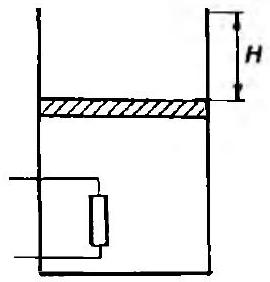
\includegraphics[max width=\textwidth, center]{2025_07_01_5b3ff9fa0d508c8e9f17g-090}

Fig. 2.9\\
2.80. Un gaz monoatomic se află într-o incintă sub presiunea unui piston de masă $M$, care se poate mişca fără frecare cu pereții incintei (Fig. 2.9).

Gazul este încălzit prin intermediul unei rezistențe electrice aflată în incintă. Dacã pistonul s-a deplasat pe distanța $H$, căldura primită de gaz este:\\
A) $Q=M g H$;\\
B) $Q=5 M g H / 2$;\\
C) $Q=5 M g H$;\\
D) $Q=3 M g H / 2$;\\
E) $Q=M g H / 2$; F) $Q=0$.\\
2.81. Într-un cilindru cu piston se află z număr $v$ de moli de He. Gazul suferă o --sformare din starea 1 în starea 2 ca în ₹ 2.10. Temperatura maximă atinsă în ---sul transformării 1-2 va fi:\\
A) $T_{\text {max }}=\frac{p_{1} V_{1}-p_{2} V_{2}}{v p_{1} V_{1}}$;\\
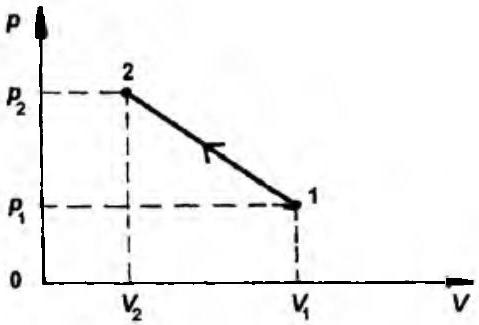
\includegraphics[max width=\textwidth, center]{2025_07_01_5b3ff9fa0d508c8e9f17g-091}

Fig. 2.10\\
B) $T_{\text {max }}=\frac{p_{2} V_{2}-p_{1} V_{1}}{v p_{2} V_{2}}$;\\
C) $T_{\text {max }}=\frac{\left(p_{2} V_{1}-p_{1} V_{2}\right)^{2}}{4 v R\left(p_{2}-p_{1}\right)\left(V_{1}-V_{2}\right)}$;\\
D) $T_{\text {max }}=\frac{\left(p_{2} V_{2}-p_{1} V_{1}\right)^{2}}{p_{2} V_{2}-p_{1} V_{1}}$; E) $T_{\text {max }}=\frac{p_{2} V_{2}}{v R}$;\\
F) $T_{\text {max }}=\frac{\left(p_{2} V_{2}-p_{1} V_{1}\right)^{2}}{v R\left(p_{2} V_{2}-p_{1} V_{1}\right)}$.\\
(Gheorghe Stanciu)\\
2.82. Un rezervor de volum $V$ este umplut cu aer la presiunea $p_{1}$ şi unperatura $T_{1}$. Rezervorul este încălzit la temperatura $T_{2},\left(T_{2}>T_{1}\right)$. Pentru ca resiunea în rezervor să rămână constantă, din rezervor este eliminată o masă $\Delta m$ こe: aer. Masa de aer rămasă în rezervor în funcție de $p_{1}, V, \mu, T_{1}, \Delta m$ este:\\
A) $m_{1}=\frac{p_{1} V}{\mu R T_{1}}-\Delta m$;\\
B) $m_{1}=\frac{p_{1} V}{R T_{2}}-\Delta m$;\\
C) $m_{1}=\frac{p_{1} T_{1}}{\mu R V}-\Delta m$;\\
D) $m_{1}=\frac{p_{1} V}{\mu T_{2}}-R \Delta m$;\\
E) $m_{1}=\frac{\mu p_{1} V}{R T_{1}}-\Delta m$;\\
F) $m_{1}=\frac{\mu p_{1} V}{R T_{1}}$.\\
(Gheorghe Stanciu)\\
2.83. În figura 2.11 punctele $A$ şi $B$ se află pe aceeaşi izotermă. Să se -recizeze dacă în cursul transformării de la A la B are loc:\\
A) o creştere a temperaturii; B) o scădere a temperaturii;\\
C) temperatura rămâne constantă;\\
D) o creştere a volumului şi o creştere a temperaturii;\\
E) o creştere şi apoi o scădere a temperaturii;\\
F) o scădere a presiunii şi o creştere a temperaturii.\\
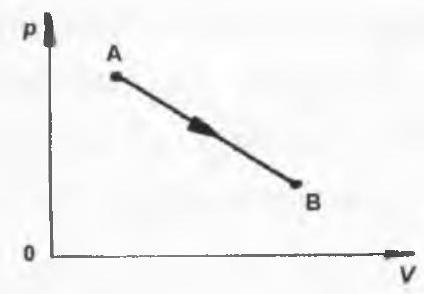
\includegraphics[max width=\textwidth, center]{2025_07_01_5b3ff9fa0d508c8e9f17g-092}

Fig. 2.11\\
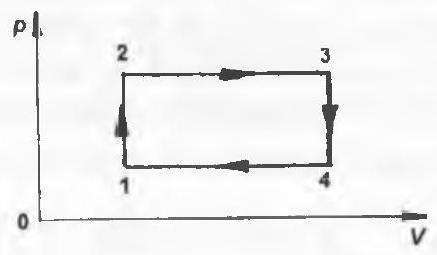
\includegraphics[max width=\textwidth, center]{2025_07_01_5b3ff9fa0d508c8e9f17g-092(1)}

Fig. 2.12\\
2.84. Un mol de gaz efectuează ciclul din Fig. 2.12. Temperaturile în punctele 1 şi 3 sunt $T_{1}$ şi respectiv $T_{3}$. ${ }^{\text {a }}$ tiind că punctele 2 şi 4 se află pe aceeaşi izotermă să se precizeze dacă lucrul efectuat pe ciclu este:\\
A) $R T_{1}\left(\sqrt{\frac{T_{3}}{T_{1}}}-1\right)$;\\
B) $R T_{1} \sqrt{\frac{T_{3}}{T_{1}}}$;\\
C) $R\left(\frac{T_{3}}{T_{1}}-1\right)$;\\
D) $R T_{1} \sqrt{\frac{T_{1}}{T_{3}}}$;\\
E) $R T_{1}\left(\sqrt{\frac{T_{1}}{T_{3}}}-1\right)^{2}$;\\
F) $R T_{1}\left(\sqrt{\frac{T_{3}}{T_{1}}}-1\right)^{2}$.\\
(Gheorghe Stanciu)\\
2.85. Un mol de gaz ideal monoatomic (coeficientul adiabatic $\gamma$ ) se află inițial într-o stare caracterizată de temperatura $T_{0}$ şi presiunea $p_{0}$. Să se determine temperatura și presiunea finală a gazului în urma unei evoluții adiabatice în care are loc o triplare a volumului ocupat de gaz.\\
A) $p=\frac{p_{0}}{3^{\gamma}}, T=3^{1-\gamma} T_{0}$;\\
B) $p=\frac{p_{0}}{3^{\gamma}}, T=3^{\gamma} T_{0}$;\\
C) $p=\frac{p_{0}}{3^{1-\gamma}}, T=3^{\gamma} T_{0}$;\\
D) $p=\frac{P_{0}}{3^{1-\gamma}}, T=3^{1-\gamma} T_{0}$;\\
E) $p=\frac{2 p_{0}}{3^{\gamma}}, T=3^{1-\gamma} T_{0}$;\\
F) $p=\frac{3 p_{0}}{3^{\gamma}}, T=3^{1-\gamma} T_{0}$.\\
(Vasile Popescu)\\
2.86. În mol de gaz ideal monoatomic (coeficientul adiabatic $\gamma$ ) se află inițial într-o stare caracterizată de temperatura $T_{0}$ şi presiunea $p_{0}$. Să se determine temperatura şi presiunea finală a gazului în urma unei evoluții izoterme în care are loc o înjumătățire a volumului ocupat de gaz.\\
A) $T=T_{0}, p=2 p_{0}$;\\
B) $T=2 T_{0}, p=2 p_{0}$;\\
C) $T=T_{0}, p=p_{0}$;\\
D) $T=2 T_{0}, p=\frac{p_{0}}{2}$;\\
E) $T=\frac{T_{0}}{2}, p=2 p_{0}$;\\
F) $T=-\frac{T_{0}}{2}, p=\frac{p_{0}}{2}$.\\
2.87. Un mol de gaz ideal monoatomic (coeficientul adiabatic $\gamma$ ) se află inițial intr-o stare caracterizată de presiunea $p_{0}$ şi volumul $V_{0}$. Să se determine lucrul mecanic în timpul unei evoluții adiabatice în care are loc o triplare a volumului ocupat de gaz.\\
A) $L=\frac{p_{0} V_{0}}{1-\gamma}\left(3^{1-\gamma}-1\right)$;\\
В) $L=\frac{p_{0} V_{0}}{1-\gamma}\left(3^{1-\gamma}+1\right)$;\\
C) $L=\frac{p_{0} V_{0}}{1-\gamma}\left(2^{1-\gamma}-1\right)$;\\
D) $L=\frac{p_{0} V_{0}}{1+\gamma}\left(3^{1-\gamma}-1\right)$;\\
E) $L=\frac{p_{0} V_{0}}{1+\gamma}\left(3^{1+\gamma}-1\right)$;\\
F) $L=\frac{p_{0} V_{0}}{1-\gamma} \cdot 3^{1-\gamma}$.\\
(Vasile Popescu)\\
2.88. Un mol de gaz ideal monoatomic (coeficientul adiabatic $\gamma$ ) se află inițial intr-o stare caracterizată de presiunea $p_{0}$ şi volumul $V_{0}$. Să se determine lucrul mecanic în timpul unei evoluții izoterme în care are loc o înjumătățire a volumului ocupat de gaz.\\
A) $L=-p_{0} V_{0} \ln 2$;\\
B) $L=-p_{0} V_{0}^{\gamma} \ln 2$;\\
C) $L=-p_{0} V_{0}^{\gamma-1} \ln 2$;\\
D) $L=-p_{0} V_{0} \ln 3$;\\
E) $L=-\frac{p_{0}}{V_{0}} \ln 2$;\\
F) $L=-\frac{p_{0} V_{0}}{\ln 2}$.\\
(Vasile Popescu)\\
2.89. Să se determine $p_{2}, T_{2}, p_{3}$ și $T_{3}$ în funcție de $p_{1}, T_{1}$ și de exponentul adiabatic $\gamma$ în cazul unui mol de gaz ideal monoatomic care este supus următoarelor transformări succesive:

$$
\begin{aligned}
& \left(p_{1}, V_{1}, T_{1}\right) \Rightarrow \frac{\text { transformare }}{\text { adiabatică }} \Rightarrow\left(p_{2}, 2 V_{1}, T_{2}\right) \Rightarrow \frac{\text { transformare }}{\text { izotermă }} \Rightarrow\left(p_{3}, V_{1}, T_{3}\right) \Rightarrow \\
& \Rightarrow \frac{\text { transformare }}{\text { izocoră }} \Rightarrow\left(p_{1}, V_{1}, T_{1}\right)
\end{aligned}
$$

A) $p_{2}=2^{-\gamma} p_{1}, T_{2}=2^{1-\gamma} T_{1}, p_{3}=\frac{p_{1}}{2^{\gamma-1}}, T_{3}=2^{1-\gamma} T_{1}$;\\
B) $p_{2}=2^{\gamma} p_{1}, T_{2}=2^{1-\gamma} T_{1}, p_{3}=2^{\gamma} p_{1}, T_{3}=2^{\gamma} T_{1}$;\\
C) $p_{2}=2^{-\gamma+1} p_{1}, T_{2}=2^{1-\gamma} T_{1}, p_{3}=2^{1-\gamma} p_{1}, T_{3}=2^{1-\gamma} T_{1}$;\\
D) $p_{2}=2^{\gamma+1} p_{1}, T_{2}=2^{\gamma+1} T_{1}, p_{3}=2^{\gamma+1} p_{1}, T_{3}=2^{\gamma+1} T_{1}$;\\
E) $p_{2}=2 p_{1}, T_{2}=2 T_{1}, p_{3}=2^{\gamma} p_{1}, T_{3}=2^{\gamma} T_{1}$;\\
F) $p_{2}=2^{-\gamma} p_{1}, T_{2}=2^{-1-\gamma} T_{1}, p_{3}=2^{-1-\gamma} p_{1}, T_{3}=2^{-1-\gamma} T_{1}$.\\
2.90. Să se determine lucrul mecanic total efectuat de un mol de gaz ideal monoatonic în următoarele transformări succesive:

$$
\left(p_{1}, V_{1}, T_{1}\right) \Rightarrow\left(p_{2}, V_{2}, T_{1}\right) \Rightarrow\left(p_{2}, V_{1}, T_{2}\right) \Rightarrow\left(p_{1}, V_{1}, T_{1}\right) .
$$

A) $p_{1} V_{1}\left(V_{2}-V_{1}\right)$; B) $p_{2}\left(V_{1}-V_{2}\right)$; C) $p_{1} V_{1} \ln \frac{V_{2}}{V_{1}}+p_{2}\left(V_{1}-V_{2}\right)$;\\
D) $p_{1} V_{1}\left(V_{2}-V_{1}\right)+p_{2}\left(V_{1}-V_{2}\right)$; E) $p_{1} V_{1} \frac{T_{2}-T_{1}}{T_{1}}$; F) $R\left(T_{2}-T_{1}\right)$.\\
(Vasile Popescu)\\
2.91. O masă de gaz $(\mu=28 \mathrm{~kg} / \mathrm{kmol}) m=1 \mathrm{~kg}$ este încălzită cu $\Delta T=100 \mathrm{~K}$ la volum constant. Să se determine variația energiei interne. Se dau: $C_{p}=\frac{7 R}{2}$, $R=8310 \mathrm{~J} / \mathrm{kmol} \cdot \mathrm{K}$.\\
A) $74,2 \mathrm{~kJ}$;\\
B) $7,79 \mathrm{MJ}$;\\
C) $7,75 \mathrm{MJ}$;\\
D) $7,4 \mathrm{~kJ}$;\\
E) 24 kJ ;\\
F) $27,5 \mathrm{~kJ}$.\\
(Vasile Popescu)\\
2.92. 1 kmol de gaz este încălzit la presiune constantă cu 10 K . Să se determine lucrul mecanic efectuat de gaz. Se dă: $R=8310 \mathrm{~J} / \mathrm{kmol} \cdot \mathrm{K}$.\\
A) $83,1 \mathrm{~kJ}$;\\
B) 831 kJ ;\\
C) 31 MJ ;\\
D) $8,31 \mathrm{~J}$;\\
E) $8,31 \mathrm{~kJ}$;\\
F) 31 kJ .\\
(Vasile Popescu)\\
2.93. Să se determine căldura primită de un gaz în cazul unei transformări ciclice în care lucrul mecanic efectuat de gaz este $L=100 \mathrm{~J}$ iar randamentul ciclului este $\eta=0,2$.\\
A) 400 J ;\\
B) 100 J ;\\
C) 500 J ;\\
D) 200 J ;\\
E) 20 J ; F) $0,002 \mathrm{~J}$.\\
(Vasile Popescu)\\
2.94. Un gaz ocupă volumul $V_{1}=1$ litru la presiunea $p_{1}=10^{5} \mathrm{~N} / \mathrm{m}^{2}$ şi temperatura $t_{1}=27^{\circ} \mathrm{C}$. Gazul este încălzit izobar până la temperatura $t_{2}=30^{\circ} \mathrm{C}$. Să se determine lucrul mecanic efectuat.\\
A) 1 J ;\\
B) 196 J ;\\
C) $9,6 \mathrm{~J}$;\\
D) 2 J ; E) 1 kJ ;\\
F) $9,6 \mathrm{~kJ}$.\\
(Vasile Popescu)\\
2.95. Un gaz ocupă volumul $V=1$ litru la presiunea $p_{1}=10^{5} \mathrm{~N} / \mathrm{m}^{2}$. Gazul este încălzit la volum constant până când presiunea sa devine $p_{2}=2 \cdot 10^{5} \mathrm{~N} / \mathrm{m}^{2}$. Să se determine căldura $Q_{V}$ absorbită de gaz.

Se dau: $C_{p}=7 R / 2, R=8310 \mathrm{~J} / \mathrm{kmol} \mathrm{K}$.\\
A) 250 J ;\\
B) 5 MJ ;\\
C) 250 J ;\\
D) 500 J ;\\
E) 250 MJ ;\\
F) $2,5 \mathrm{~J}$.\\
(Vasile Popescu)\\
2.96. Un gaz ideal monoatomic ( $C_{V}=3 / 2 R$ ) se destinde după legea $p=a V$, unde $a=10^{8} \mathrm{~N} \cdot \mathrm{~m}^{-5}$, de la volumul $V_{1}=2 \cdot 10^{-3} \mathrm{~m}^{3}$ până la volumul $V_{2}=2 V_{1}$. Cât este căldura în această tranformare ?\\
A) $2,4 \mathrm{~kJ}$;\\
B) 51000 J ;\\
C) 10000 J ;\\
D) 100 J ;\\
E) 10 kJ ;\\
F) 1 kJ .\\
(Niculae N. Puşcaş)\\
2.97. În interiorul unui balon cu volumul $0,1 \mathrm{~m}^{3}$ se aflã un gaz la presiunea $2 \cdot 10^{5} \mathrm{~N} / \mathrm{m}^{2}$ şi temperatura 400 K . Balonul este răcit până la temperatura 300 K , presiunea gazului devenind $10^{5} \mathrm{~N} / \mathrm{m}^{2}$, iar $54,6 \mathrm{~g}$ de gaz a ieşit din balon printr-o supapă. Cât este densitatea gazului în condiții normale ?\\
$\left(p_{0}=10^{5} \mathrm{~N} / \mathrm{m}^{2} ; T_{0}=273 \mathrm{~K}\right)$\\
A) $5 \mathrm{~kg} / \mathrm{m}^{3}$;\\
B) $1,2 \mathrm{~kg} / \mathrm{m}^{3}$;\\
C) $0,1 \mathrm{~kg} / \mathrm{m}^{3}$;\\
D) $100 \mathrm{~kg} / \mathrm{m}^{3}$;\\
E) $10,2 \mathrm{~kg} / \mathrm{m}^{3}$;\\
F) $12 \mathrm{~kg} / \mathrm{m}^{3}$.\\
(Niculae N. Puşcaş)\\
2.98. Cât este lucrul mecanic efectuat de $v$ kmoli de gaz perfect când se dilată de la $T_{1}$ la $T_{2}$ ştiind că temperatura acestuia variază proporțional cu pătratul presiunii ? Se dă $R$.\\
A) $\frac{1}{2} v R\left(T_{2}-T_{1}\right)$;\\
В) $\frac{5}{2} \nu R\left(T_{1}-T_{2}\right)$;\\
C) $\frac{5}{2} v R\left(T_{2}-T_{1}\right)$;\\
D) $R\left(T_{2}-T_{1}\right)$;\\
E) $\frac{1}{2} v\left(T_{2}-T_{1}\right)$;\\
F) $\frac{1}{2} v R\left(2 T_{2}-T_{1}\right)$.\\
(Niculae N. Puşcaş)\\
2.99. În trei vase având volumele de 3 litri, 5 litrişi respectiv 2 litri se află trei gaze diferite la aceeaşi temperatură, presiunile corespunzătoare fiind $2 \cdot 10^{5} \mathrm{~N} / \mathrm{m}^{2}, 3 \cdot 10^{5} \mathrm{~N} / \mathrm{m}^{2}$ şi $5 \cdot 10^{5} \mathrm{~N} / \mathrm{m}^{2}$.

Cât este presiunea finală a amestecului dacă cele trei vase sunt legate între ele prin tuburi de volume neglijabile?\\
A) $3,64 \mathrm{~N} / \mathrm{m}^{2}$;\\
B) $3,1 \cdot 10^{5} \mathrm{~N} / \mathrm{m}^{2}$;\\
C) $1,12 \mathrm{~N} / \mathrm{m}^{2}$;\\
D) $7,41 \cdot 10^{5} \mathrm{~N} / \mathrm{m}^{2}$;\\
E) $20 \mathrm{~N} / \mathrm{m}^{2}$;\\
F) $4,8 \cdot 10^{5} \mathrm{~N} / \mathrm{m}^{2}$.\\
2.100. Cât este variația energiei interne a 2 g de gaz ideal $\left(C_{V}=\frac{3}{2} R\right)$ pentru care în urma încălzirii viteza termică inițială de $400 \mathrm{~m} / \mathrm{s} ~ \mathrm{~s}-\mathrm{a}$ dublat ?\\
A) 100 J ;\\
B) 10 J ;\\
C) 2000 J ;\\
D) 10 kJ ;\\
E) 480 J ;\\
F) 5000 J .

2.101. O maşină termică ideală funcționează după un ciclu Carnot, temperatura sursei reci find 300 K , iar a celei calde cu 100 K mai mult. Cât este căldura cedată sursei reci ştiind că în timpul unui ciclu motorul efectuează un lucru mecanic de $0,1 \mathrm{~kJ}$ ?\\
A) 100 J ;\\
B) 1000 J ;\\
C) 2 kJ ;\\
D) 300 J ;\\
E) 5 kJ ;\\
F) $0,9 \mathrm{~kJ}$.\\
(Niculae N. Puşcaş)\\
2.102. Două corpuri de fier $A$ şi $B$ se pun în contact termic. Corpul $A$ are masa $m_{\mathrm{A}}$ şi temperatura $t_{\mathrm{A}}=900^{\circ} \mathrm{C}$, iar corpul B are masa $m_{\mathrm{B}}=2 m_{\mathrm{A}}$ şi temperatura $t_{\mathrm{B}}=t_{\mathrm{A}} / 2$. Temperatura finală de echilibru va fi:\\
A) $600^{\circ} \mathrm{C}$;\\
B) $650^{\circ} \mathrm{C}$;\\
C) $700^{\circ} \mathrm{C}$;\\
D) $750^{\circ} \mathrm{C}$;\\
E) $800^{\circ} \mathrm{C}$;\\
F) $850^{\circ} \mathrm{C}$.\\
(Mircea Stan)\\
2.103. Un vas cilindric are un capac de greutate 5 N şi diametru 20 cm . În vas se află vapori (considerați drept gaz ideal) la temperatura de $41^{\circ} \mathrm{C}$ şi presiunea de $10^{5} \mathrm{~N} / \mathrm{m}^{2}$. La ce temperatură încep vaporii să iasă afară din vas ?\\
A) $90^{\circ} \mathrm{C}$;\\
B) $80,5^{\circ} \mathrm{C}$;\\
C) $71,5^{\circ} \mathrm{C}$;\\
D) $51^{\circ} \mathrm{C}$;\\
E) $50,5^{\circ} \mathrm{C}$; F) $41,5^{\circ} \mathrm{C}$.\\
(Mircea Stan)\\
2.104. La $0^{\circ} \mathrm{C}$ densitatea uleiului este $840 \mathrm{~kg} / \mathrm{m}^{3}$. Care va fi densitatea uleiului încălzit la o temperatură la care volumul său a crescut cu $20 \%$ ?\\
A) $830 \mathrm{~kg} / \mathrm{m}^{3}$;\\
B) $820 \mathrm{~kg} / \mathrm{m}^{3}$;\\
C) $720 \mathrm{~kg} / \mathrm{m}^{3}$;\\
D) $700 \mathrm{~kg} / \mathrm{m}^{3}$;\\
E) $680 \mathrm{~kg} / \mathrm{m}^{3}$;\\
F) $660 \mathrm{~kg} / \mathrm{m}^{3}$.\\
(Mircea Stan)\\
2.105. Care este energia cinetică medie de translație a tuturor moleculelor de aer dintr-un pahar de apă cu volumul 0,25 litri aflat la presiunea $p=10^{5} \mathrm{~Pa}$ ?\\
A) $2,25 \mathrm{~J}$;\\
B) $37,5 \mathrm{~J}$;\\
C) $18,9 \mathrm{~J}$;\\
D) $20,25 \mathrm{~J}$;\\
E) $21,4 \mathrm{~J}$;\\
F) $22,38 \mathrm{~J}$.\\
(Mircea Stan)\\
2.106. Un gaz ideal monoatomic ( $C_{V}=\frac{3}{2} R$ ) primeşte căldura $Q=12,45 \mathrm{~kJ}$ pentru a-şi mări izocor temperatura $\Delta T$. Ce căldură ar fỉ necesară gazului pentru z-şi mări temperatura tot cu $\Delta T$, dar intr-o transformare izobară ?\\
A) $63,35 \mathrm{~kJ}$;\\
B) $52,55 \mathrm{~kJ}$;\\
C) $41,52 \mathrm{~kJ}$;\\
D) $30,15 \mathrm{~kJ}$;\\
E) $25,5 \mathrm{~kJ}$; F) $20,75 \mathrm{~kJ}$.\\
(Mircea Stan)\\
2.107. Ce lucru mecanic efectuează un gaz ideal în urma transformării ciclice ABC din Fig. 2.13?

Se cunosc: $p_{\mathrm{A}}=p_{\mathrm{C}}=1 \mathrm{~atm} ; \quad V_{\mathrm{A}}=1,5$ litri; $V_{\mathrm{C}}=2,5$ litri; $p_{\mathrm{B}}=3$ atm.\\
A) $1,5 \mathrm{~kJ}$;\\
B) 100 J ;\\
C) 3 kJ ;\\
D) $3,5 \mathrm{~kJ}$;\\
E) $4,5 \mathrm{~kJ}$;\\
F) $5,5 \mathrm{~kJ}$.\\
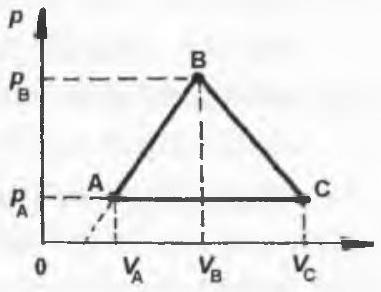
\includegraphics[max width=\textwidth, center]{2025_07_01_5b3ff9fa0d508c8e9f17g-097}

Fig. 2.13\\
(Mircea Stan)\\
2.108. Randamentul unei maşini termice ideale este de $40 \%$. Cât devine randamentul dacă temperatura izvorului cald creşte de trei ori, iar temperatura izvorului rece se reduce la jumătate ?\\
A) $35 \%$;\\
B) $48 \%$;\\
C) $50 \%$;\\
D) $70 \%$;\\
E) $90 \%$;\\
F) $95 \%$.\\
(Mircea Stan)\\
2.109. Ce lucru mecanic efectuează un gaz diatomic $\left(C_{V}=\frac{5}{2} R\right)$ care primeşte izobar căldura $Q=14,7 \mathrm{~kJ}$ ?\\
A) $4,2 \mathrm{~kJ}$;\\
B) $6,1 \mathrm{~kJ}$;\\
C) $8,2 \mathrm{~kJ}$;\\
D) $9,7 \mathrm{~kJ}$;\\
E) $10,4 \mathrm{~kJ}$;\\
F) $11,2 \mathrm{~kJ}$.\\
(Mircea Stan)\\
2.110. Un cilindru cu sectiunea $S=3 \mathrm{~cm}^{2}$ este acoperit cu un piston de greutate neglijabilă, asupra căruia apasă forța $F=20,64 \mathrm{~N}$. În interiorul vasului se află un gaz ideal cu densitatea $\rho=1,29 \mathrm{~kg} / \mathrm{m}^{3}$. Viteza termică a moleculelor de gaz este:\\
A) $120 \mathrm{~m} / \mathrm{s}$;\\
B) $200 \mathrm{~m} / \mathrm{s}$;\\
C) $320 \mathrm{~m} / \mathrm{s}$;\\
D) $400 \mathrm{~m} / \mathrm{s}$;\\
E) $420 \mathrm{~m} / \mathrm{s}$;\\
F) $500 \mathrm{~m} / \mathrm{s}$.\\
(Mircea Stan)\\
2.111. O moleculă de heliu ( $\mu_{\mathrm{He}}=4$ ) are masa $m=6,6 \cdot 10^{-27} \mathrm{~kg}$. Ce masă are o moleculă de magneziu ? $\left(\mu_{\mathrm{Mg}} \approx 24\right)$\\
A) $8,4 \cdot 10^{-27} \mathrm{~kg}$;\\
B) $6,21 \cdot 10^{-26} \mathrm{~kg}$;\\
C) $3,96 \cdot 10^{-26} \mathrm{~kg}$;\\
D) $4,54 \cdot 10^{-27} \mathrm{~kg}$;\\
E) $6,86 \cdot 10^{-27} \mathrm{~kg}$;\\
F) $4,18 \cdot 10^{-26} \mathrm{~kg}$.\\
(Mircea Stan)\\
2.112. Căldura schimbată cu exteriorul de sistemele termodinamice în cursul transformărilor de stare:\\
A) este schimbată în mod izocor cu exteriorul;\\
B) raportată la masa de substanţă transformată este egală cu o constantă de material specifică transformării considerate;\\
C) trebuie măsurată direct, fiind imposibilă calcularea ei datorită modificării coeficienților calorici ai sistemului în cursul transformărilor de fază;\\
D) este o măsură a energiei de agitație termică;\\
E) se numeşte căldură latentă a transformării pentru că aceste transformări sunt, în general, transformări de durată;\\
F) este schimbată în mod izobar cu exteriorul.\\
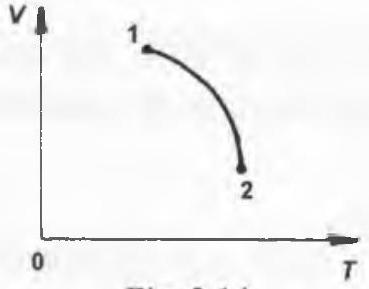
\includegraphics[max width=\textwidth, center]{2025_07_01_5b3ff9fa0d508c8e9f17g-098}

Fig. 2.14\\
2.113. Conform Fig. 2.14, dacă presiunea $p=c t$., ce se poate spune despre masa gazului dacă densitatea gazului rămâne constantă ?\\
A) creşte; B) depinde de presiune;\\
C) rămâne constantă;\\
D) depinde de pătratul presiunii;\\
E) scade; F) creşte şi apoi scade.\\
(Elena Slavnicu)\\
2.114. Cunoscând presiunea $p=55 \mathrm{kPa}$ şi viteza pătratică medie a moleculelor de azot $v_{T}=550 \mathrm{~m} / \mathrm{s}$, concentrația moleculelor şi densitatea gazului sunt:\\
A) $n=10^{25} \mathrm{~m}^{-3} ; \rho=0,465 \mathrm{~kg} / \mathrm{m}^{3}$;\\
B) $n=10^{4} \mathrm{~m}^{-3} ; \rho=0,500 \mathrm{~kg} / \mathrm{m}^{3}$;\\
C) $n=5 \cdot 10^{25} \mathrm{~m}^{-3} ; \rho=0,290 \mathrm{~kg} / \mathrm{m}^{3}$;\\
D) $n=10^{25} \mathrm{~m}^{-3} ; \rho=0,545 \mathrm{~kg} / \mathrm{m}^{3}$;\\
E) $n=1,2 \cdot 10^{25} \mathrm{~m}^{3} ; \rho=0,549 \mathrm{~kg} / \mathrm{m}^{3}$;\\
F) $n=10^{-24} \mathrm{~m}^{3} ; \rho=0,455 \mathrm{~kg} / \mathrm{m}^{3}$.\\
(Elena Slavnicu)\\
2.115. Două baloane legate printr-un tub subțire, prevăzut cu un robinet, conțin aer la aceeaşi temperatură. Volumul primului balon este de $n$ ori mai mare decât volumul celui de-al doilea. Presiunea în primul balon este $4 \cdot 10^{4} \mathrm{~N} / \mathrm{m}^{2}$. Masa aerului din balonul al doilea este de $k$ ori mai mare decât în primul. Presiunea care se stabileşte în baloane, dacă deschidem robinetul, este (se dau $n=3,5 ; k=4$ ):\\
A) 180 kPa ;\\
B) $170 \mathrm{~N} / \mathrm{m}^{2}$;\\
C) $155,6 \mathrm{kN} / \mathrm{m}^{2}$;\\
D) $720 \mathrm{~N} / \mathrm{m}^{2}$;\\
E) $72 \mathrm{~N} / \mathrm{m}^{2}$;\\
F) 175 kPa .\\
(Elena Slavnicu)\\
2.116. Două gaze diferite aflate la temperaturi diferite sunt în contact termic şi izolate de exterior. În acest caz, care din următoarele afirmații este adevărată:\\
A) gazele vor rămâne la temperaturi diferite;\\
B) gazele vor ajunge la aceeaşi densitate;\\
C) gazele vor ajunge la aceeaşi concentrație a moleculelor;\\
D) gazele vor ajunge la aceeaşi energie cinetică medie de translație a unei molecule;\\
E) gazele vor ajunge la aceeaşi viteză pătratică medie a moleculelor;\\
F) nici una din variantele anterioare nu este corectă.\\
(Elena Slavnicu)\\
2.117. Care din următoarele afirmații este în contradicție cu principiul al doilea al termodinamicii?\\
A) lucrul mecanic se poate transforma integral în căldură;\\
B) randamentul maxim al unui motor termic este subunitar;\\
C) căldura se poate transforma integral în lucru mecanic, într-un proces ciclic, reversibil;\\
D) nu este posibilă o transformare care să aibă ca rezultat trecerea căldurii de la un corp cu o temperatură dată, la altul de aceeaşi temperatură;\\
E) se poate construi o maşină care să transforme căldura în lucru mecanic;\\
F) într-o transformare ciclică, monotermă, sistemul nu poate ceda lucru mecanic în exterior.\\
(Elena Slavnicu)\\
2.118. Un mol de gaz ideal monoatomic se răceşte izocor astfel încât presiunea scade de k ori, apoi gazul se destinde izobar astfel încât volumul său creşte de $k$ ori. Să se găsească valoarea lui $k$ dacă în aceste transformări s-a transmis gazului o căldură egală cu jumătate din energia internă inițială a gazului.\\
A) $k=1 / 2$;\\
B) $k=8$;\\
C) $k=4$;\\
D) $k=3$;\\
E) $k=2$;\\
F) $k=\sqrt{2}$.\\
(Elena Slavnicu)\\
2.119. Un gaz închis într-o incintă de volum $V$, aflat la temperatura $T=300 \mathrm{~K}$ şi presiunea $p=2 \mathrm{~atm}$, suferă un proces termodinamic în urma căruia temperatura scade cu $\Delta T=30 \mathrm{~K}$ iar volumul creşte cu $n=20 \%$. Presiunea finală va fi:\\
A) $p=3 \mathrm{~atm}$; B) $p=1,5 \mathrm{~atm}$;\\
C) $p=4 \mathrm{~atm}$; D) $p=3,5 \mathrm{~atm}$;\\
E) presiunea rămâne neschimbată; F) $p=3,6 \mathrm{~atm}$.\\
(Constantin Roşu)\\
2.120. Un gaz ideal biatomic parcurge ciclul din Fig. 2.15. Ştiind că $V_{2}=e \cdot V_{1} \quad$ şi $\quad T_{3}=2 \cdot T_{2} \quad(e \quad$ este baza\\
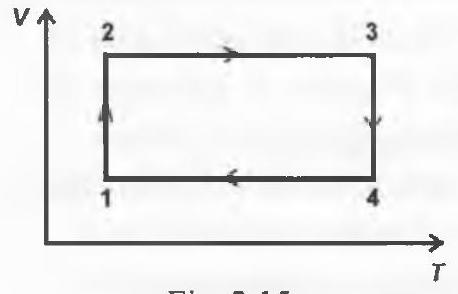
\includegraphics[max width=\textwidth, center]{2025_07_01_5b3ff9fa0d508c8e9f17g-100}

Fig. 2.15 logaritmilor naturali), să se calculeze randamentul ciclului.\\
A) $\eta=\frac{2}{5} ;$\\
B) $\eta=\frac{2}{9}$;\\
C) $\eta=50 \%$;\\
D) $\eta=\frac{3}{5}$;\\
E) $\eta=\frac{1}{4} ; \mathrm{F}$\\
F) $\eta=\frac{3}{4}$\\
(Constantin Roşu)\\
2.121. Un motor termic cu randamentul $\eta_{1}$ acționează un dinam cu puterea utilă $P$ şi randamentul $\eta_{2}$. Să se calculeze căldura oferită de motorul termic sistemului său de răcire în timpul $t$.\\
A) $Q_{\text {racire }}=\frac{P \cdot t \cdot\left(1+\eta_{1}\right)}{\eta_{1} \cdot \eta_{2}}$;\\
B) $Q_{\text {racire }}=\frac{P \cdot t \cdot \eta_{1} \cdot \eta_{2}}{\eta_{1}+\eta_{2}}$;\\
C) $Q_{\text {racire }}=\frac{(P-t)}{\eta_{1} \cdot \eta_{2}}$;\\
D) $Q_{\text {racire }}=\frac{P \cdot t \cdot \sqrt{\eta_{1}}}{\eta_{1} \cdot \eta_{2}}$;\\
E) $Q_{\text {racire }}=\frac{P \cdot t \cdot\left(1-\eta_{1}\right)}{\eta_{1} \cdot \eta_{2}}$;\\
F) $Q_{\text {racire }}=\frac{P \cdot t \cdot\left(1-\eta_{1}\right)}{2 \eta_{1} \cdot \eta_{2}}$.\\
(Constantin Roşu)\\
2.122. Se pun în contact termic 4 corpuri din acelaşi material de temperaturi inițiale $t_{1}=10^{\circ} \mathrm{C}, t_{2}=20^{\circ} \mathrm{C}, t_{3}=30^{\circ} \mathrm{C}, t_{4}=50^{\circ} \mathrm{C}$ şi mase $m_{1}=2 \mathrm{~kg}, m_{2}=0,5 \mathrm{~kg}$, $m_{3}=I \mathrm{~kg}$ şi $m_{4}=3 \mathrm{~kg}$. Atunci temperatura finală a amestecului va fi:\\
A) $t=27,5^{\circ} \mathrm{C}$;\\
B) $t=41,8^{\circ} \mathrm{C}$;\\
C) $t=32,3{ }^{\circ} \mathrm{C}$;\\
D) $t=56^{\circ} \mathrm{C}$;\\
E) $t=42,4^{\circ} \mathrm{C}$;\\
F) $t=22,5^{\circ} \mathrm{C}$.\\
(Constantin Roşu)\\
2.123. Un perpetuum mobile de speța I reprezintă:\\
A) o maşină termică care produce lucru mecanic de la o singură sursă de căldură; B) un motor Carnot; C) un motor care funcționează cu energie nucleară; D) o maşină termică care efectuează lucru mecanic fără consum de energie din\\
exterior; E) o maşină termică bitermă; F) un ansamblu motor cu benzină plus dinam electric.\\
(Constantin Roşu)\\
2.124. Intre masa $m$ a unei molecule, masa molară $\mu$ a unui gaz constanta lui Boltzmann şi constanta gazelor perfecte $R$, există relația:\\
A) $\mu \cdot k=\sqrt{\frac{R}{m}}$;\\
В) $\mu \cdot k=m \cdot R$;\\
C) $\mu / k=m / R$;\\
D) $\mu^{2}=m \cdot R / k$;\\
E) $\mu+k=m-R$;\\
F) $\mu / k=m \cdot R$.\\
(Constantin Roşu)\\
2.125. Lucrul mecanic efectuat de un sistem izolat adiabatic de exterior depinde numai de:\\
A) variația presiunii sistemului între starea inițială și finală; B) raportul dintre cāldura cedată şi primită de sistem; C) stările intermediare din prima jumătate a procesului; D) starea inițială şi finală a sistemului; E) logaritmul raportului dintre volumul final, respectiv inițial; F) temperatura sistemului, dar nu depinde de presiune.\\
(Constantin Roşu)\\
2.126. Într-un cilindru cu piston se află aer la presiunea $p_{1}=2 \cdot 10^{5} \mathrm{~N} / \mathrm{m}^{2}$ şi temperatura $T_{1}=300 \mathrm{~K}$. Să se afle masa unei greutăți care trebuie pusă deasupra pistonului, pentru ca volumul aerului să rămână constant, dacă gazul din piston este încălzit până la temperatura $T_{2}=333 \mathrm{~K}$. Secțiunea pistonului este $S=3 \cdot 10^{-3} \mathrm{~m}^{2}$. Se dă: $g=10 \mathrm{~m} / \mathrm{s}^{2}$.\\
A) $6,6 \mathrm{~g}$;\\
B) 36 kg ;\\
C) $6,6 \mathrm{~kg}$;\\
D) 8 kg ;\\
E) $4,6 \mathrm{~kg}$;\\
F) $0,1 \mathrm{~kg}$.\\
(Răzvan Mitroi)\\
2.127. Să se afle căldurile specifice $c_{V}$ şi $c_{p}$ ale unui gaz ideal, ştiind masa moleculară $\mu=30 \mathrm{~kg} / \mathrm{kmol}$ şi coeficientul adiabatic $\gamma=1,4$.

Se dă: $R=8,31 \mathrm{~J} / \mathrm{molK}$.\\
A) $c_{V}=692,5 \mathrm{~J} / \mathrm{kg} \cdot \mathrm{K}, c_{p}=692,5 \mathrm{~J} / \mathrm{kg} \cdot \mathrm{K}$;\\
B) $c_{V}=250 \mathrm{~J} / \mathrm{kg} \cdot \mathrm{K}, c_{p}=692,5 \mathrm{~J} / \mathrm{kg} \cdot \mathrm{K}$;\\
C) $c_{V}=692,5 \mathrm{~J} / \mathrm{kg} \cdot \mathrm{K}, c_{p}=969,5 \mathrm{~J} / \mathrm{kg} \cdot \mathrm{K}$;\\
D) $c_{V}=392,5 \mathrm{~J} / \mathrm{kg} \cdot \mathrm{K}, c_{p}=372 \mathrm{~J} / \mathrm{kg} \cdot \mathrm{K}$;\\
E) $c_{V}=392,5 \mathrm{~J} / \mathrm{kg} \cdot \mathrm{K}, c_{p}=692,5 \mathrm{~J} / \mathrm{kg} \cdot \mathrm{K}$;\\
F) $c_{V}=30 \mathrm{~J} / \mathrm{kg} \cdot \mathrm{K}, c_{p}=38,31 \mathrm{~J} / \mathrm{kg} \cdot \mathrm{K}$.\\
(Răzvan Mitroi)\\
2.128. Într-un ciclu Carnot de randament $\eta=40 \%$, lucrul mecanic efectuat de gaz la destinderea izotermă este $L_{i z o t}=100 \mathrm{~J}$. Care este lucrul mecanic consumat de gaz la comprimarea izotermă ?\\
A) 60 W ;\\
B) 100 J ;\\
C) 260 W ;\\
D) 50 J ;\\
E) 60 J ;\\
F) 6 J .\\
(Rǎzvan Mitroi)\\
2.129. La ce temperatură viteza pătratică medie a moleculelor de azot se dublează față de valoarea de la temperatura $t_{0}=0^{\circ} \mathrm{C}$.\\
А) 1000 K ;\\
B) $819^{\circ} \mathrm{C}$;\\
C) 273 K ;\\
D) $1000^{\circ} \mathrm{C}$;\\
E) 500 K ;\\
F) $100^{\circ} \mathrm{C}$.\\
(Rǎzvan Mitroi)\\
2.130. Ce masă de oxigen s-a consumat dintr-o butelie de volum $V=60$ litri dacă presiunea inițială a fost $p_{1}=10^{7} \mathrm{~N} / \mathrm{m}^{2}$ la temperatura $t_{1}=27^{\circ} \mathrm{C}$, iar presiunea finala a devenit $p=29 \cdot 10^{5} \mathrm{~N} / \mathrm{m}^{2}$ la temperatura $t_{2}=17^{\circ} \mathrm{C}$.

Se dau: $\mu_{\text {aer }}=32 \mathrm{~kg} / \mathrm{kmol}, R=8,31 \mathrm{~J} / \mathrm{mol} \cdot \mathrm{K}$.\\
A) $4,2 \mathrm{~kg}$;\\
B) $5,39 \mathrm{~kg}$;\\
C) 2 kg ;\\
D) $1,8 \mathrm{~kg}$;\\
E) $5,39 \mathrm{~g}$;\\
F) 8 kg .\\
(Răzvan Mitroi)\\
2.131. Un vas cilindric orizontal care este împărțit de un piston termoizolant, inițial blocat, în două părți de volume $V_{1}=1$ litru şi $V_{2}=2$ litri, conține gaz la presiunile $p_{1}=3 \cdot 10^{5} \mathrm{~N} / \mathrm{m}^{2}$ şi respectiv $p_{2}=10^{5} \mathrm{~N} / \mathrm{m}^{2}$ la aceeaşi temperatură. Pistonul este lăsat liber, iar gazul din primul compartiment este încălzit până la temperatura $T_{1}=400 \mathrm{~K}$, iar cel din al doilea compartiment este încălzit până la temperatura $T_{2}=300 \mathrm{~K}$. Cât va fi volumul fiecărui compartiment?\\
A) $2 \cdot 10^{-3} \mathrm{~m}^{3}, 2 \cdot 10^{-3} \mathrm{~m}^{3}$;\\
B) $10^{-3} \mathrm{~m}^{3}, 4 \cdot 10^{-3} \mathrm{~m}^{3}$;\\
C) $3 \cdot 10^{-3} \mathrm{~m}^{3}, 10^{-3} \mathrm{~m}^{3}$;\\
D) $10^{-3} \mathrm{~m}^{3}, 10^{-3} \mathrm{~m}^{3}$;\\
E) $2 \cdot 10^{-3} \mathrm{~m}^{3}, 10^{-3} \mathrm{~m}^{3}$;\\
F) $3 \cdot 10^{-3} \mathrm{~m}^{3}, 7 \cdot 10^{-3} \mathrm{~m}^{3}$.\\
(Răzvan Mitroi)\\
2.132. Un balon având volumul $V=10^{-2} \mathrm{~m}^{3}$ contine oxigen la presiunea $p=10^{6} \mathrm{~N} / \mathrm{m}^{2}$ şi la temperatura $t=7^{\circ} \mathrm{C}$. Ce cantitate de căldură absoarbe gazul dacă este încălzit până la $17^{\circ} \mathrm{C}$, ştiind că densitatea oxigenului la $0^{\circ} \mathrm{C}$ este $1,43 \mathrm{~kg} / \mathrm{m}^{3}$, iar căldura specifică $921 \mathrm{~J} / \mathrm{kg} \cdot$ grad.

Se va considera presiunea atmosfericǎ la $0^{\circ} \mathrm{C}, p_{0}=10^{5} \mathrm{~N} / \mathrm{m}^{2}$.\\
A) 280 J ;\\
$\mathrm{B}) 100 \mathrm{~J}$;\\
D) 1800 J ;\\
D) 1280 J ;\\
E) 500 J ; F) 640 J .\\
(Răzvan Mitroi)\\
2.133. Într-un cilindru vertical cu piston se află aer la presiunea atmosferică normală $p_{0}=10^{5} \mathrm{~N} / \mathrm{m}^{2}$. Pistonul de masă neglijabilă şi secțiunea $S=200 \mathrm{~cm}^{2}$ se află inițial la distanța $d_{1}=1,6 \mathrm{~m}$ de fundul cilindrului, apoi este adus încet la distanța $d_{2}=10 \mathrm{~cm}$. Să se determine forța $F$ ce acționează asupra pistonului aflat în poziția finală. Frecările se neglijează.\\
A) 15 N ; B) 30 N ; C) 15 kN ; D) 30 kN ; E) 50 N ; F) 10 kN .\\
(Tatiana Pop)\\
2.134. O masă $m=10 \mathrm{~g}$ de oxigen se află la presiunea $p=3 \cdot 10^{5} \mathrm{~N} / \mathrm{m}^{2}$ şi la temperatura $t_{1}=10^{\circ} \mathrm{C}$. După o încălzire izobară, gazul ocupă volumul $V_{2}=10$ litri. Cunoscând masa molară a oxigenului $\mu=32 \mathrm{~kg} / \mathrm{kmol}$, căldura molară izobară $C_{p}=7 R / 2$ şi constanta universală a gazelor perfecte $R=8310 \mathrm{~J} / \mathrm{kmol} \cdot \mathrm{K}$, atunci căldura absorbită de gaz şi variația energiei interne a gazului au valorile :\\
A) $Q=7927,8 \mathrm{~J}, \Delta U=5662,8 \mathrm{~J}$;\\
B) $Q=5662,8 \mathrm{~J}, \Delta U=7927,8 \mathrm{~J}$;\\
C) $Q=9727,8 \mathrm{~J}, \Delta U=2565,8 \mathrm{~J}$;\\
D) $Q=7927,8 \mathrm{~J}, \Delta U=0$;\\
E) $Q=0 \mathrm{~J}, \Delta U=0 \mathrm{~J}$;\\
F) $Q=-79,275 \mathrm{~J}, \Delta U=56,65 \mathrm{~J}$.\\
(Tatiana Pop)\\
2.135. Randamentul unui ciclu format din două izobare şi două izocore cu $p=2 p_{0}$ şi $V_{1}=V_{0}$ şi $p_{3}=p_{0}$ şi $V_{3}=3 V_{0}$, parcurs de un gaz ideal biatomic cu $C_{V}=5 R / 2$ este:\\
A) $50 \%$;\\
В) $36,4 \%$;\\
C) $24,24 \%$;\\
D) $12,12 \%$;\\
E) $75 \%$;\\
F) $1,2 \%$.\\
(Tatiana Pop)\\
2.136. Un mol de gaz ideal se găseşte în starea $A$, caracterizată prin temperatura $t_{A}=47^{\circ} \mathrm{C}$. Gazul trece într-o stare $B$, printr-o încălzire izobară\\
producând un lucru mecanic $L=1662 \mathrm{~J}$. Se cere temperatura $T_{B}$ din starea finală, $R=8,31 \mathrm{~J} / \mathrm{mol} \cdot \mathrm{K}$.\\
A) 520 K ;\\
В) 150 K ;\\
C) 300 K ;\\
D) 100 K ;\\
E) 700 K ;\\
F) 820\\
K.\\
(Tatiana Pop)\\
2.137. Temperatura unui gaz scade izocor de la valoarea $T_{1}=400 \mathrm{~K}$ la $T_{2}=200 \mathrm{~K}$. Cu cât la sută scade presiunea gazului:\\
A) $10 \%$;\\
B) $20 \%$;\\
C) $70 \%$;\\
D) $45 \%$;\\
E) $50 \%$; F) $30 \%$.\\
(Ion Belciu)\\
2.138. O maşină termică funcționând după un ciclu Carnot între temperaturile $T_{1}=400 \mathrm{~K}$ şi $T_{2}=300 \mathrm{~K}$, produce într-un ciclu lucrul mecanic $L=80 \mathrm{~kJ}$. Căldura cedată sursei reci într-un ciclu este:\\
A) 100 kJ ;\\
B) 250 kJ ;\\
C) 40 kJ ;\\
D) 240 kJ ;\\
E) 120 kJ ;\\
F) 152 kJ .\\
(Ion Belciu)\\
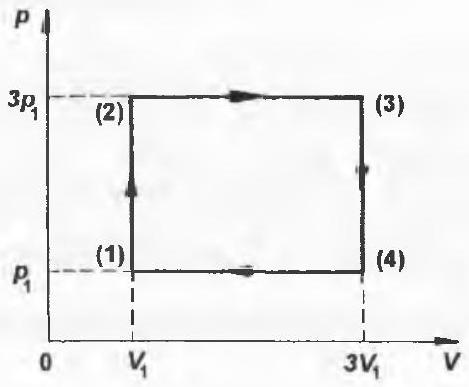
\includegraphics[max width=\textwidth, center]{2025_07_01_5b3ff9fa0d508c8e9f17g-104}

Fig. 2.16\\
2.139. O maşină termică funcționează cu gaz ideal biatomic ( $C_{V}=\frac{5}{2} R$ ) după ciclul din Fig. 2.16. Randamentul maşinii termice este:\\
A) $\frac{2}{3}$;\\
B) $\frac{15}{40}$;\\
C) $\frac{16}{30}$;\\
D) $\frac{20}{75}$;\\
E) $\frac{2}{13}$;\\
F) $\frac{5}{17}$.\\
(Ion Belciu)\\
2.140. O pompă de vid de volum $V_{0}$ trebuie să micşoreze presiunea aerului dintr-un vas cu volumul $V$ de la presiunea $p_{0}$ la presiunea $p=10^{-4} p_{0}$.

Considerând temperatura constantă, numărul curselor făcute de pompă va fi:\\
A) $10^{-4} \frac{p}{p_{0}}$;\\
B) $10^{-4} \frac{V_{0}+V}{V}$;\\
C) $\frac{\lg \left(\frac{V+V_{0}}{V}\right)}{5}$;\\
D) $4 \ln \frac{V_{0}}{V}$;\\
E) $\frac{4}{\lg \left(\frac{V+V_{0}}{V}\right)}$;\\
F) $4 \frac{p_{0}}{p}$.\\
2.141. Presiunea unui gaz creşte de patru ori prin încălzire izocoră. Raportul vitezelor termice ale moleculelor de gaz înainte şi după încălzire este:\\
А) 4;\\
B) 2 ;\\
C) $\frac{1}{4}$;\\
D) $\frac{1}{2}$;\\
E) $\frac{1}{16}$;\\
F) $\frac{1}{5}$.\\
(Ion Belciu)\\
2.142. O bară de oțel cu secţiunea $S=10 \mathrm{~cm}^{2}$, având modulul de elasticitate $E=2 \cdot 10^{11} \mathrm{~N} / \mathrm{m}^{2}$ şi coeficientul de dilatare volumică $\gamma=33 \cdot 10^{-6} \mathrm{~K}^{-1}$, este fixată la capete de un suport rigid. Crescând temperatura barei cu $\Delta T=100 \mathrm{~K}$, forța cu care apasă bara asupra suportului va fi:\\
A) $10^{9} \mathrm{~N}$;\\
B) $3 \cdot 10^{10} \mathrm{~N}$;\\
C) $27 \cdot 10^{8} \mathrm{~N}$;\\
D) $22 \cdot 10^{4} \mathrm{~N}$;\\
E) $3 \cdot 10^{7} \mathrm{~N}$;\\
F) $52 \cdot 10^{5} \mathrm{~N}$.\\
(Ion Belciu)\\
2.143. Se amestecă o cantitate de apă cu temperatura $t_{1}=40^{\circ} \mathrm{C}$ cu o cantitate triplă de apă cu temperatura $t_{2}=60^{\circ} \mathrm{C}$. Temperatura finală a amestecului de apă va fi:\\
A) $42^{\circ} \mathrm{C}$;\\
B) $50^{\circ} \mathrm{C}$;\\
C) $30^{\circ} \mathrm{C}$;\\
D) $55^{\circ} \mathrm{C}$;\\
E) $58^{\circ} \mathrm{C}$;\\
F) $45^{\circ} \mathrm{C}$.\\
(Ion Belciu)\\
2.144. În interiorul unui cilindru orizontal, izolat adiabatic față de exterior, se găseşte în compartimentul A (Fig. 2.17) o cantitate $v$ dintr-un gaz ideal la temperatura $t_{\mathrm{A}}=127^{\circ} \mathrm{C}$, ocupând un volum delimitat de peretele fix $M$, ce permite schimbul de\\
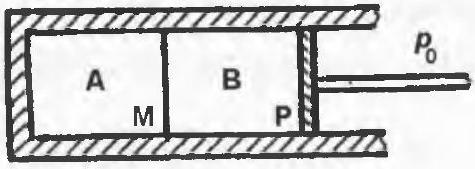
\includegraphics[max width=\textwidth, center]{2025_07_01_5b3ff9fa0d508c8e9f17g-105}

Fig. 2.17 căldură cu compartimentul B , în care se găseşte aceeaşi cantitate $v$ din acelaşi gaz, la presiunea atmosferică $p_{0}$ şi temperatura inițială $t_{\mathrm{B}}=27^{\circ} \mathrm{C}$, volumul acestui compartiment fiind variabil prin deplasarea pistonului $P$ ce se poate mişca fară frecare. În exteriorul cilindrului presiunea aerului este $p_{0}$, iar căldura molară la volum constant a gazului din compartimentele A şi B este $\frac{3}{2} R$. După un timp se ajunge la echilibru termodinamic, temperatura din ambele compartimente fiind $T_{f}$ :\\
А) $387,5 \mathrm{~K}$;\\
В) 350 K ;\\
C) $337,5 \mathrm{~K}$;\\
D) $327,5 \mathrm{~K}$;\\
E) 316 K ; F) $302,5 \mathrm{~K}$.\\
2.145. Prin încălzirea masei $m=2 \cdot 10^{-3} \mathrm{~kg}$ de gaz ideal diatomic, viteza termică a crescut de la $v_{T_{1}}=400 \mathrm{~m} / \mathrm{s}$ la $v_{T_{2}}=500 \mathrm{~m} / \mathrm{s}$. Se cere variația energiei interne a cantității respective de gaz, ştiind $C_{V}=\frac{5}{2} R$.\\
A) 225 J ;\\
B) 360 J ;\\
C) 150 J ;\\
D) 600 J ;\\
E) 900 J ;\\
F) 1200 J .\\
(Corneliu Călin)\\
2.146. Procesul ciclic efectuat de o cantitate de gaz ideal monoatomic se reprezintă (Fig. 2.18) prin dreapta 1-2 (a cărei prelungire trece prin 0), prin izocora $2-3$ urmată de izobara $3-1$. Ştiind căldura molară în transformarea $1-2$ : $C_{12}=2 R$ şi raportul $\frac{V_{2}}{V_{1}}=2$, se cere randamentul $\eta$ al acestui ciclu şi randamentul $\eta_{c}$ al unui ciclu Carnot care ar evolua între aceleaşi limite extreme de temperaturi:\\
A) $\eta=\frac{1}{12}, \eta_{c}=\frac{3}{4}$;\\
B) $\eta=\frac{1}{6}, \eta_{c}=\frac{3}{4}$;\\
C) $\eta=\frac{2}{3}, \eta_{c}=\frac{3}{4}$;\\
D) $\eta=\frac{1}{8}, \eta_{c}=\frac{1}{2}$;\\
E) $\eta=\frac{1}{6}, \eta_{c}=\frac{1}{2}$;\\
F) $\eta=\frac{1}{3}, \eta_{c}=\frac{2}{3}$.\\
(Corneliu Călin)\\
\includegraphics[max width=\textwidth, center]{2025_07_01_5b3ff9fa0d508c8e9f17g-106}

Fig. 2.18\\
2.147. Cantitatea de 1 kmol de gaz ideal efectuează un ciclu Carnot între temperaturile $t_{1}=227^{\circ} \mathrm{C}$ şi $t_{2}=27^{\circ} \mathrm{C}$, raportul volumelor în procesul destinderii izoterme find $\varepsilon=10$. Se cere lucrul mecanic efectuat în cursul ciclului. Se consideră constanta gazelor $R=8,31 \mathrm{~J} / \mathrm{mol} \mathrm{K}$.\\
A) $3,818 \mathrm{MJ}$;\\
B) $9,545 \mathrm{MJ}$;\\
C) $5,727 \mathrm{MJ}$;\\
D) $3,818 \mathrm{~kJ}$;\\
E) $9,545 \mathrm{~kJ}$;\\
F) $5,725 \mathrm{~kJ}$.\\
(Corneliu Călin)\\
2.148. Într-o incintă se află azot la presiunea $p=10^{5} \mathrm{~Pa}$. Care este concentrația moleculelor de azot dacă viteza pătratică medie a acestora este $v=10^{4} \mathrm{~m} / \mathrm{s}$ ?\\
A) $1,5 \cdot 10^{15} \mathrm{~m}^{-3}$;\\
B) $\frac{3}{5} \cdot 10^{20} \mathrm{~m}^{-3}$;\\
C) $\frac{9}{14} \cdot 10^{23} \mathrm{~m}^{-3}$;\\
D) $7 \cdot 10^{22} \mathrm{~m}^{-3}$;\\
E) $\frac{8}{3} \cdot 10^{18} \mathrm{~m}^{-3}$;\\
F) $10^{24} \mathrm{~m}^{-3}$.\\
(Marin Cilea)\\
2.149. Intr-o butelie de volum $V=83,1$ litri se aflã heliu la presiunea $p=2,9 \cdot 10^{5} \mathrm{~Pa}$ şi temperatura $T_{1}=290 \mathrm{~K}$. După ce din butelie s-a mai scos heliu, presiunea a devenit $p_{2}=1,25 \cdot 10^{5} \mathrm{~Pa}$, iar temperatura $T_{2}=250 \mathrm{~K}$. Cu cât a scăzut masa heliului din butelie?\\
A) 15 g ;\\
B) $1,5 \mathrm{~g}$;\\
C) 100 g ;\\
D) 20 g ;\\
E) 85 g ; F) 44 g .\\
(Marin Cilea)\\
2.150. O masă de azot $m=6,73 \mathrm{~g}$ este încălzită cu $\Delta T=200 \mathrm{~K}$ la volum constant. Să se afle căldura $Q_{V}$ absorbită $\left(C_{V}=\frac{5}{2} R\right)$.\\
A) 100 J ;\\
B) 2500 J ;\\
C) 1000 J ;\\
D) 4 kJ ;\\
E) $2,2 \mathrm{~kJ}$; F) 200 J .\\
(Marin Cilea)\\
2.151. Un gaz ocupă volumul $V_{1}=10^{-2} \mathrm{~m}^{3}$ la presiunea $p_{1}=2,9 \cdot 10^{5} \mathrm{~Pa}$ şi temperatura $T_{1}=290 \mathrm{~K}$. Gazul este încǎlzit izobar şi efectuează un lucru mecanic $L=200 \mathrm{~J}$. Să se afle cu cât s-a încălzit gazul.\\
A) 20 K ;\\
B) 10 K ;\\
C) 100 K ;\\
D) 45 K ;\\
E) 550 K ;\\
F) 300 K .\\
(Marin Cilea)\\
2.152. Într-un recipient de volum $V=2 \cdot 10^{-2} \mathrm{~m}^{3}$ se află hidrogen la presiunea $p_{1}=10^{5} \mathrm{~Pa}$. Gazul este încălzit la volum constant până când presiunea sa devine $P_{2}=2 \cdot 10^{5} \mathrm{~Pa}$. Să se afle variația energiei interne $\left(C_{V}=\frac{5}{2} R\right)$.\\
A) 2 kJ ;\\
B) $5 \cdot 10^{3} \mathrm{~J}$;\\
C) 4 kJ ;\\
D) $12,1 \mathrm{~kJ}$;\\
E) 200 J ;\\
F) 800 J .\\
(Marin Cilea)\\
2.153. Un gaz efectuează o transformare ciclică în timpul căreia primeşte de la sursa caldă căldura $Q_{1}=4 \mathrm{~kJ}$. Să se afle lucrul mecanic efectuat de gaz într-un ciclu dacã randamentul acestuia este $\eta=0,25$.\\
A) 750 J ;\\
B) 1 kJ ;\\
C) 3 kJ ;\\
D) $1,2 \mathrm{~kJ}$;\\
E) 950 J ; F) 500 J .\\
(Marin Cilea)\\
2.154. Într-un kilogram de apă cu temperatura de $10^{\circ} \mathrm{C}$ se pun $4,181 \mathrm{~kg}$ dintr-un metal cu temperatura de $80^{\circ} \mathrm{C}$. Temperatura de echilibru a amestecului este de $40^{\circ} \mathrm{C}$. Care este căldura specifică a metalului? ( $c_{\text {apă }}=4181 \mathrm{~J} / \mathrm{kg} \cdot \mathrm{K}$ )\\
A) $225 \mathrm{~J} / \mathrm{kg} \cdot \mathrm{K}$;\\
B) $410 \mathrm{~J} / \mathrm{kg} \cdot \mathrm{K}$;\\
C) $10^{3} \mathrm{~J} / \mathrm{kg} \cdot \mathrm{K}$;\\
D) $750 \mathrm{~J} / \mathrm{kg} \cdot \mathrm{K}$;\\
E) $550 \mathrm{~J} / \mathrm{kg} \cdot \mathrm{K}$;\\
F) $760 \mathrm{~J} / \mathrm{kg} \cdot \mathrm{K}$.\\
2.155. Într-un cilindru orizontal ìmpărțit în două compartimente (cu ajutorul unui piston care se poate mişca făă frecări) se găsesc două cantități de gaze diferite $m_{1}$, respectiv $m_{2}$, de mase molare $\mu_{1}$ şi $\mu_{2}$, la temperaturile $T_{1}$ şi $T_{2}$. Raportul volumelor este:\\
A) $\frac{V_{1}}{V_{2}}=\frac{m_{1}}{m_{2}} \cdot \frac{T_{1}}{T_{2}} \cdot \frac{\mu_{1}}{\mu_{2}}$;\\
В) $\frac{V_{1}}{V_{2}}=\frac{m_{2}}{m_{1}} \cdot \frac{T_{2}}{T_{1}} \cdot \frac{\mu_{1}}{\mu_{2}}$;\\
C) $\frac{V_{1}}{V_{2}}=\frac{m_{2}}{m_{1}} \cdot \frac{T_{1}}{T_{2}} \cdot \frac{\mu_{2}}{\mu_{1}}$;\\
D) $\frac{V_{1}}{V_{2}}=\frac{m_{1}}{m_{2}} \cdot \frac{T_{1}}{T_{2}} \cdot \frac{\mu_{2}}{\mu_{1}}$;\\
E) $\frac{V_{1}}{V_{2}}=\frac{m_{1}}{m_{2}} \cdot \frac{T_{2}}{T_{1}} \cdot \frac{\mu_{1}}{\mu_{2}}$;\\
F) $\frac{V_{1}}{V_{2}}=\frac{m_{1}}{m_{2}} \cdot \frac{T_{2}}{T_{1}} \cdot \frac{\mu_{2}}{\mu_{1}}$.\\
(Ilie Ivanov)\\
2.156. Un recipient de volum $V$ conține gaz la presiunea $p_{0}$ şi la temperatura $T_{1}$. Dacă se încălzeşte sistemul până la o temperatură $T_{2}>T_{1}$, iese afară o masă $\Delta m$ care asigură menținerea unei presiuni $p=p_{0}$. Densitatea $\rho_{0}$ a gazului în condiții normale se exprimă prin relația:\\
A) $\rho_{0}=\frac{\Delta m\left(T_{2}-T_{1}\right)}{T_{1} T_{0} V}$;\\
B) $\rho_{0}=V \Delta m$;\\
C) $\rho_{0}=\frac{T_{1} T_{2} \Delta m}{\sqrt{T_{0}}\left(T_{2}-T_{1}\right)}$;\\
D) $\rho_{0}=\frac{2 T_{1} T_{2} \Delta m}{\left(T_{1}+T_{2}\right) V T_{0}}$;\\
E) $\rho_{0}=\frac{\Delta m\left(T_{1}-T_{2}\right)}{T_{1} T_{0} V}$;\\
F) $\rho_{0}=\frac{T_{0}\left(T_{1}-T_{2}\right)}{T_{1} T_{2}} \frac{\Delta m}{V}$.\\
(Ilie Ivanov)\\
2.157. Un mol de He dintr-un recipient de volum $V=22$ litri este încălzit cu $\Delta T=10 \mathrm{~K}$ presiunea crescând de 10 ori. Temperatura inițială $T_{1}$ este:\\
A) 11 K ;\\
В) $0,1 \mathrm{~K}$;\\
C) $1,1 \mathrm{~K}$;\\
D) 111 K ;\\
E) $2,2 \mathrm{~K}$;\\
F) 22 K .\\
(Ilie Ivanov)\\
2.158. Într-un recipient izolat adiabatic de mediul exterior se găsesc două gaze monoatomice ideale, separate printr-un perete adiabatic. Temperaturile lor sunt $T_{1}$, respectiv $T_{2}$, iar cantitățile de substanță $v_{1}$, respectiv $v_{2}$. Dacă se scoate peretele dintre ele sau dacă acesta este poros, atunci în urma difuziei temperatura de echilibru va fi:\\
A) $T=\frac{v_{1} T_{1}+v_{2} T_{2}}{2 \sqrt{v_{1} v_{2}}}$;\\
B) $T=\sqrt{T_{1} T_{2}} \sqrt{\frac{v_{1} v_{2}}{v_{1}+v_{2}}}$;\\
C) $T=\frac{v_{1} T_{1}+v_{2} T_{2}}{v_{1}+v_{2}}$;\\
D) $T=\frac{2 v_{1} v_{2}}{v_{1}+v_{2}} \cdot \frac{T_{1}+T_{2}}{2}$;\\
E) $T=\frac{v_{1} T_{2}+v_{2} T_{1}}{v_{1}+v_{2}}$;\\
F) $\left(\frac{1}{v_{1}}+\frac{1}{v_{2}}\right) \cdot \frac{T_{1} T_{2}}{T_{1}+T_{2}}\left(v_{1}+v_{2}\right)$.\\
2.159. Într-un vas de sticlă cu coeficientul de dilatație volumică $\gamma$ se găseşte $o$ masă de apă $m$ atunci când este plin la temperatura $t_{0}=0^{\circ} \mathrm{C}$. Prin încălzire până la temperatura $t$, o parte din lichid curge şi rămâne masa $m^{\prime}<m$. Se cere coeficientul de dilatare volumică al apei, $\gamma_{a}$.\\
A) $\gamma_{a}=\gamma$;\\
B) $\gamma_{a}=\gamma \frac{m-m^{\prime}}{m^{\prime}}$;\\
C) $\gamma_{a}=\gamma \frac{m \gamma t-m^{\prime}}{m^{\prime} t}$;\\
D) $\gamma_{a}=\frac{m-m^{\prime}+m \gamma t}{m^{\prime} t}$;\\
E) $\gamma_{a}=\frac{\left(m-m^{\prime}\right) y t-m^{\prime}}{m t}$;\\
F) $\gamma_{a}=\gamma \frac{m-m^{\prime}}{m}$.\\
(Ilie Ivanov)\\
2.160. În care dintre procesele reprezentate in Fig. 2.19 lucrul mecanic schimbat de sistem (gaz ideal) este cel mai mic? Toate procesele au loc între aceleaşi stări, notate cu 1 (inițială) şi 2 (finală).\\
A) în $a ; B$ ) în $b ; C$ ) în $c ; D$ ) în $d ; E$ ) în $e$;\\
F) în toate procesele lucrul mecanic este acelaşi.\\
(Eugen Scarlat)\\
\includegraphics[max width=\textwidth, center]{2025_07_01_5b3ff9fa0d508c8e9f17g-109(1)}

Fig. 2.19\\
\includegraphics[max width=\textwidth, center]{2025_07_01_5b3ff9fa0d508c8e9f17g-109}

Fig. 2.20\\
2.161. În care dintre procesele reprezentate în Fig. 2.20, variația energiei interne este cea mai mică? Toate procesele au loc între starea inițială 1 şi starea finală 2.\\
A) în $a$; B) în b; C) în c; D) în d; E) în e;\\
F) în toate procesele variația energiei interne este aceeaşi.\\
(Eugen Scarlat)\\
2.162. În care dintre transformările izobare, reprezentate în Fig. 2.21, ale unei cantități fixate de gaz ideal, presiunea este cea mai mică? În toate stările inițiale temperatura este $T_{1}$ şi în toate stările finale temperatura este $T_{2}$.\\
A) în $a$; B) în b; C) în c; D) în d; E) în e;\\
F) în toate procesele reprezentate presiunea este aceeaşi.\\
2.163. În care dintre transformǎrile izocore, reprezentate în Fig. 2.22, ale unei cantități fixate de gaz ideal, volumul este cel mai mic? În toate stările inițiale temperatura este $T_{1}$ şi în toate stările finale temperatura este $T_{2}$.\\
A) în a; B) în b; C) în c; D) în d; E) în e;\\
F) în toate procesele reprezentate volumul este acelaşi.\\
(Eugen Scarlat)\\
\includegraphics[max width=\textwidth, center]{2025_07_01_5b3ff9fa0d508c8e9f17g-110(3)}

Fig. 2.21\\
\includegraphics[max width=\textwidth, center]{2025_07_01_5b3ff9fa0d508c8e9f17g-110(2)}

Fig. 2.22\\
2.164. În care dintre transformările reprezentate în Fig. 2.23, ale unei cantități fixate de gaz ideal, variația energiei interne este cea mai mică? În toate stările inițiale temperatura este $T_{1}$ şi în toate stările finale temperatura este $T_{2}$.\\
A) în $\mathrm{a} ; \mathrm{B}$ ) în $\mathrm{b} ; \mathrm{C}$ ) în $\mathrm{c} ; \mathrm{D}$ ) în d ; E) în e ;\\
F) în toate procesele reprezentate variația energiei interne este aceeaşi.\\
(Eugen Scarlat)\\
\includegraphics[max width=\textwidth, center]{2025_07_01_5b3ff9fa0d508c8e9f17g-110}

Fig. 2.23\\
\includegraphics[max width=\textwidth, center]{2025_07_01_5b3ff9fa0d508c8e9f17g-110(1)}

Fig. 2.24\\
2.165. În care dintre procesele reprezentate în Fig. 2.24 căldura schimbată de sistem (gaz ideal) este cea mai mică? Toate procesele au loc între aceleaşi stări, notate cu 1 (inițială) şi 2 (finală).\\
A) în $a ; B$ ) în $b ; C$ ) în $c ; D$ ) în d; E) în e; F) în f;\\
G) în toate procesele reprezentate căldura schimbată este aceeaşi.\\
2.166. În care dintre procesele reprezentate în Fig. 2.25 căldura schimbată de sistem (gaz ideal) este cea mai mică? Toate procesele au loc între aceleaşi stări, potate cu 1 (initială) şi 2 (finală).\\
A) în $\mathrm{a} ; \mathrm{B}$ ) în $\mathrm{b} ; \mathrm{C}$ ) în $\mathrm{c} ; \mathrm{D}$ ) în $\mathrm{d} ; \mathrm{E}$ ) în e ;\\
F) în toate procesele reprezentate căldura schimbată este aceeaşi.\\
(Eugen Scarlat)\\
\includegraphics[max width=\textwidth, center]{2025_07_01_5b3ff9fa0d508c8e9f17g-111}

Fig. 2.25\\
\includegraphics[max width=\textwidth, center]{2025_07_01_5b3ff9fa0d508c8e9f17g-111(1)}

Fig. 2.26\\
2.167. În care dintre procesele reprezentate în Fig. 2.26 lucrul mecanic schimbat de sistem (gaz ideal) este cel mai mic? Toate procesele au loc între aceleaşi stări, notate cu 1 (inițială) şi 2 (finală).\\
A) în $a$; B) în b; C) în c; D) în d; E) în e;\\
F) în toate procesele reprezentate lucrul mecanic schimbat este acelaşi.\\
(Eugen Scarlat)\\
2.168. Într-un gram de dioxid de carbon există un număr de molecule egal cu:\\
А) $1,36 \times 10^{20}$;\\
В) $3.61 \times 10^{21}$;\\
C) $1,36 \times 10^{22}$;\\
D) $6,31 \times 10^{22}$;\\
E) $3.61 \times 10^{22}$;\\
F) $6,023 \times 10^{23}$.\\
(Mihai Cristea)\\
2.169. Un gaz aflat în condiții normale de temperatură şi presiune, are densitatea $\rho=1,25 \mathrm{mg} / \mathrm{cm}^{3}$. Acest gaz este:\\
A) He ;\\
B) $\mathrm{H}_{2}$;\\
C) $\mathrm{C}_{2} \mathrm{H}_{2}$;\\
D) $\mathrm{N}_{2}$;\\
E) $\mathrm{CO}_{2}$; F) $\mathrm{O}_{2}$\\
(Mihai Cristea)\\
2.170. Un gaz ideal $\left(C_{V}=\frac{3}{2} R\right)$ suferă o destindere izobară. Lucrul mecanic efectuat în cursul acestui proces reprezintă un procent din căldura primită egal cu:\\
А) $40 \%$;\\
B) $60 \%$;\\
C) $80 \%$;\\
D) $50 \%$;\\
E) $20 \%$; F) $30 \%$.\\
2.171. Un motor termic ce funcționează după un ciclu Carnot are randamentul $\eta=50 \%$. Un alt motor Carnot are temperatura sursei reci de două ori mai mare decât temperatura sursei reci a primului motor. Ştiind cǎ diferența dintre temperatura sursei calde şi temperatura sursei reci este aceeaşi în cazul ambelor motoare, atunci randamentul celui de-al doilea motor termic este:\\
A) $25 \%$;\\
B) $33,33 \%$;\\
C) $50 \%$;\\
D) $66,66 \%$;\\
Е) $75 \%$;\\
F) $88,88 \%$.\\
(Mihai Cristea)\\
2.172. O masă constantă de gaz ideal suferă o transformare în care viteza pătratică medie depinde de concentrația particulelor prin relația $\overline{v^{2}} \cdot n=c t$. Această transformare este:\\
A) izotermă; B) izocoră; C) izobară; D) adiabatică; E) oarecare;\\
F) nu reprezintă nici o transformare termodinamică.\\
(Mihai Cristea)\\
\includegraphics[max width=\textwidth, center]{2025_07_01_5b3ff9fa0d508c8e9f17g-112}

Fig. 2.27\\
2.173. Un gaz ideal monoatomic parcurge ciclul din Fig. 2.27, unde transformarea $2 \rightarrow 3$ este adiabatică, iar transformarea $3 \rightarrow 1$ este izotermă. ${ }^{\text {a }}$ tiind că $V_{2}=\frac{V_{1}}{2}$, să se calculeze randamentul acestui ciclu în funcție de randamentul unui ciclu Carnot ce ar funcționa între temperaturile extreme atinse pe acest ciclu.\\
A) $\eta=1-\frac{\eta_{c}}{\ln \left(1-\eta_{c}\right)}$;\\
B) $\eta=1-\frac{2 \eta_{c}}{\ln 2-\frac{3}{2} \ln \left(1-\eta_{c}\right)}$;\\
C) $\eta=1-\frac{\eta_{c}}{2 \ln 2}$;\\
D) $\eta=1-\frac{2 \ln \left(1+\eta_{c}\right)}{3 \ln 2}$;\\
E) $\eta=\frac{1}{2} \eta_{c} ; \quad$ F) $\eta=1-\frac{\ln \left(1+\eta_{c}\right)}{\eta_{c}}$.\\
(Mihai Cristea)\\
2.174. Un mol de gaz ideal monoatomic trece dintr-o stare 1 în starea finală 4 conform graficului din Fig. 2.28. Căldura totală schimbată de gaz cu mediul exterior, dacă diferența dintre temperatura finală şi cea inițială este de $\Delta T=100 \mathrm{~K}$. este egală cu ( $C_{V}=3 R / 2, R=8310 \mathrm{~J} / \mathrm{kmol} \mathrm{K}$ ):\\
A) $3 \mathrm{R} / 20 \mathrm{~J}$;\\
B) $5 \mathrm{R} / 20 \mathrm{~J}$;\\
C) $7 \mathrm{R} / 20 \mathrm{~J}$;\\
D) $3 \mathrm{R} / 40 \mathrm{~J}$;\\
E) $5 \mathrm{R} / 40 \mathrm{~J}$;\\
F) $7 \mathrm{R} / 40 \mathrm{~J}$.\\
2.175. Un gaz ideal monoatomic de masă $m=80 \mathrm{~g}$ şi masă molară - $=40 \mathrm{~g} / \mathrm{mol}$ este încălzit într-un cilindru cu piston, astfel încât temperatura lui variază proporțional cu pătratul presiunii $\left(T \sim p^{2}\right)$ de la valoarea inițială $T_{1}=300 \mathrm{~K}$ până la temperatura finalǎ $T_{2}=400 \mathrm{~K}$. Lucrul mecanic efectuat de gaz în timpul procesului şi cantitatea de căldură transmisă gazului au valorile ( $R=8310 \mathrm{~J} / \mathrm{kmol} \mathrm{K}$ ):\\
A) $380 \mathrm{~J} ; 2,3 \mathrm{~kJ}$;\\
B) $330 \mathrm{~J} ; 3,6 \mathrm{~kJ}$;\\
C) $730 \mathrm{~J} ; 6,3 \mathrm{~kJ}$;\\
D) $871 \mathrm{~J} ; 4 \mathrm{~kJ}$;\\
E) $831 \mathrm{~J} ; 0,831 \mathrm{~kJ}$;\\
F) $831 \mathrm{~J} ; 3,324 \mathrm{~kJ}$.\\
(Daniela Buzatu)\\
2.176. În Fig. 2.29 sunt prezentate două cicluri închise: $1 \rightarrow 2 \rightarrow 3$ şi $1 \rightarrow 3 \rightarrow 4$. Amândouă ciclurile sunt efectuate de câte un mol de gaz ideal monoatomic. Calculați raportul randamentelor celor două cicluri $\eta(1 \rightarrow 2 \rightarrow 3) / \eta(1 \rightarrow 3 \rightarrow 4)$.\\
А) $22 / 20$;\\
B) $25 / 24$;\\
C) $24 / 23$;\\
D) $24 / 22$;\\
E) $21 / 23$;\\
F) $25 / 23$.\\
(Daniela Buzatu)\\
\includegraphics[max width=\textwidth, center]{2025_07_01_5b3ff9fa0d508c8e9f17g-113(1)}

Fig. 2.28\\
\includegraphics[max width=\textwidth, center]{2025_07_01_5b3ff9fa0d508c8e9f17g-113}

Fig. 2.29\\
2.177. Un vas termoizolant este despărțit în două compartimente cu ajutorul unui perete. Într-o parte se aflǎ $v_{1}$ moli de oxigen $\mathrm{O}_{2}$ la temperatura $T_{1}$, iar în cealaltă parte se află $v_{2}$ moli de azot $\mathrm{N}_{2}$ la temperatura $T_{2}$. Temperatura stabilită în amestecul de gaze după ce peretele a fost îndepărtat este: $\left(C_{V}\left(\mathrm{O}_{2}\right)=C_{V}\left(\mathrm{~N}_{2}\right)\right)$\\
A) $\left(v_{1} T_{1}-v_{2} T_{2}\right) /\left(v_{1}-v_{2}\right)$;\\
B) $\left(v_{2} T_{1}-v_{1} T_{2}\right) /\left(v_{1}-v_{2}\right)$;\\
C) $\left(v_{1} T_{1}+v_{2} T_{2}\right) /\left(v_{1}-v_{2}\right)$;\\
D) $\left(v_{1} T_{1}+v_{2} T_{2}\right) /\left(v_{1}+v_{2}\right)$;\\
E) $\left(v_{2} T_{2}-v_{1} T_{1}\right) /\left(v_{1}+v_{2}\right)$;\\
F) $\left(v_{2} T_{2}-v_{1} T_{1}\right) /\left(v_{1}-v_{2}\right)$.\\
(Daniela Buzatu)\\
2.178. Un gaz ideal care efectuează un ciclu Carnot cedează unui frigider $70 \%$ din căldura primită pe ciclu. Temperatura sursei calde este $T_{1}=400 \mathrm{~K}$. Temperatura frigiderului va fi:\\
A) 120 K ;\\
B) 260 K ;\\
C) 140 K ;\\
D) 380 K ;\\
E) 220 K ;\\
F) 280 K .\\
(Daniela Buzatu)\\
2.179. Un gaz care are coeficientul adiabatic $\gamma=1,4$ ocupă volumul $V=3 \mathrm{dm}^{3}$ şi se găseşte la presiunea $p=0,2 \mathrm{MPa}$. În urma unei încălziri izobare volumul său creşte de 3 ori. Să se calculeze cantitatea de căldură folosită la încălzire.\\
A) 3600 J ; B) 2000 J ;\\
C) 420 J ;\\
D) 4200 J ;\\
E) 200 J ;\\
F) 8400 J .\\
(Ileana Creangă)\\
2. 180. În timpul unui proces termodinamic, un sistem primeşte o cantitate de cădură de 210 kJ şi în acelaşi timp sistemul se destinde la o presiune exterioară constantă de $0,8 \cdot 10^{5} \mathrm{~N} / \mathrm{m}^{2}$. Energia internă a sistemului se menține constantă în timpul procesului. Cât este variația volumului sistemului ?\\
A) $2,625 \mathrm{~m}^{3}$;\\
B) $26 \mathrm{~m}^{3}$;\\
C) $2,5 \mathrm{~m}^{3}$;\\
D) $54 \mathrm{~m}^{3}$;\\
E) $1,7 \mathrm{~m}^{3}$;\\
F) $1,425 \mathrm{~m}^{3}$.\\
(Ileana Creangă)\\
2.181. Să se afle căldurile specifice ale unui gaz cunoscând coeficientul adiabatic $\gamma=1,4$ și densitatea gazului în condiții normale $\rho_{0}=1,293 \mathrm{~kg} / \mathrm{m}^{3}$.

Se dau: $p_{0}=10^{5} \mathrm{~N} / \mathrm{m}^{2} ; T_{0}=273 \mathrm{~K}$.\\
A) $c_{V}=77,4 \mathrm{~J} / \mathrm{kg} \cdot \mathrm{K} ; c_{p}=1004,36 \mathrm{~J} / \mathrm{kg} \cdot \mathrm{K}$;\\
B) $c_{V}=174 \mathrm{~J} / \mathrm{kg} \cdot \mathrm{K} ; c_{p}=369 \mathrm{~J} / \mathrm{kg} \cdot \mathrm{K}$;\\
C) $c_{V}=717,4 \mathrm{~J} / \mathrm{kg} \cdot \mathrm{K} ; c_{p}=1004,36 \mathrm{~J} / \mathrm{kg} \cdot \mathrm{K}$;\\
D) $c_{V}=185 \mathrm{~J} / \mathrm{kg} \cdot \mathrm{K} ; c_{p}=1004,36 \mathrm{~J} / \mathrm{kg} \cdot \mathrm{K}$;\\
E) $c_{V}=217,4 \mathrm{~J} / \mathrm{kg} \cdot \mathrm{K} ; c_{p}=3004,3 \mathrm{~J} / \mathrm{kg} \cdot \mathrm{K}$;\\
F) $c_{V}=1 \mathrm{~J} / \mathrm{kg} \cdot \mathrm{K} ; c_{p}=1,4 \mathrm{~J} / \mathrm{kg} \cdot \mathrm{K}$.\\
(Ileana Creangă)\\
2.182. Într-un recipient se găsesc 10 kg de oxigen la temperatura inițială de $27^{\circ} \mathrm{C}$. Să se afle cantitatea de căldură ce trebuie furnizată gazului într-o transformare izocoră pentru a dubla viteza pătratică medie a moleculelor gazului.

Se dau: $C_{\nu}=\frac{5}{2} R ; R=8,31 \mathrm{~J} / \mathrm{mol} \cdot \mathrm{K}, \mu=32 \mathrm{~kg} / \mathrm{kmol}$.\\
A) 500 kJ ;\\
B) $58,4 \mathrm{~kJ}$;\\
C) 840 kJ ;\\
D) 520 kJ ;\\
E) $5842,9 \mathrm{~kJ}$; F\\
F) $55,8 \mathrm{~J}$.\\
(Ileana Creangă)\\
2.183. O masă $m=20 \mathrm{~g}$ de aer se dilată izobar la presiunea $p=2 \cdot 10^{5} \mathrm{~N} / \mathrm{m}^{2}$ de la o temperatură initială $t_{1}=17^{\circ} \mathrm{C}$ până la o temperatură finală $t_{2}=300^{\circ} \mathrm{C}$. Să se afle densitățile în stările (1) şi (2). Se dau: $\mu_{\text {aer }}=29 \mathrm{~kg} / \mathrm{kmol}, R=8,31 \mathrm{~J} / \mathrm{mol} \cdot \mathrm{K}$.\\
A) $\rho_{1}=2 \mathrm{~kg} / \mathrm{m}^{3}, \rho_{2}=2,2 \mathrm{~kg} / \mathrm{m}^{3}$;\\
B) $\rho_{1}=2,40 \mathrm{~kg} / \mathrm{m}^{3}, \rho_{2}=1,26 \mathrm{~kg} / \mathrm{m}^{3}$;\\
C) $\rho_{1}=4 \mathrm{~kg} / \mathrm{m}^{3}, \rho_{2}=12 \mathrm{~kg} / \mathrm{m}^{3}$;\\
D) $\rho_{1}=2,40 \mathrm{~g} / \mathrm{m}^{3}, \rho_{2}=1,22 \mathrm{~g} / \mathrm{m}^{3}$;\\
E) $\rho_{1}=3,40 \mathrm{~kg} / \mathrm{m}^{3}, \rho_{2}=7,22 \mathrm{~kg} / \mathrm{m}^{3}$;\\
F) $\rho_{1}=0,25 \mathrm{~kg} / \mathrm{m}^{3}, \rho_{2}=1,22 \mathrm{~kg} / \mathrm{m}^{3}$.\\
(Ileana Creangă)\\
2.184. Ce masă de oxigen s-a consumat dintr-o butelie de volum $V=60$ litri dacă presiunea inițială a fost $p_{1}=10^{7} \mathrm{~N} / \mathrm{m}^{2}$ la temperatura $t_{1}=27^{\circ} \mathrm{C}$, iar presiunea finală a devenit $p=29 \cdot 10^{5} \mathrm{~N} / \mathrm{m}^{2}$ la $t_{2}=17^{\circ} \mathrm{C}$.

Se dau: $\mu_{\mathrm{O}_{2}}=32 \mathrm{~kg} / \mathrm{kmol}, R=8,31 \mathrm{~J} / \mathrm{mol} \cdot \mathrm{K}$.\\
A) $5,39 \mathrm{~kg}$;\\
B) $7,9 \mathrm{~g}$;\\
C) $1,39 \mathrm{~kg}$;\\
D) $3,9 \mathrm{~kg}$;\\
E) $5,39 \mathrm{~g}$;\\
F) $1,63 \mathrm{~kg}$.\\
(Ileana Creangă)\\
2.185. Un vas cilindric împarțit de un piston termoizolant, inițial blocat, în două volume $V_{1}=3$ litri, $V_{2}=1$ litru conține gaz la presiunile $p_{1}=2 \cdot 10^{5} \mathrm{~N} / \mathrm{m}^{2}$, respectiv $p_{2}=10^{5} \mathrm{~N} / \mathrm{m}^{2}$ aflat la aceeaşi temperatură. Pistonul este deblocat şi gazul având volumul $V_{1}$ este încălzit până când temperatura sa absolută devine de $n=1,5$ ori mai mare decât cea inițială. Cu cât va creşte volumul $V_{1}$ ?\\
A) $0,6 \cdot 10^{-3} \mathrm{~cm}^{3}$;\\
B) $2 \cdot 10^{-3} \mathrm{~m}^{3}$;\\
C) $7,6 \mathrm{~m}^{3}$;\\
D) $0,6 \cdot 10^{-3} \mathrm{~m}^{3}$;\\
D) $10^{-3} \mathrm{~m}^{3}$.\\
E) $6 \cdot 10^{-3} \mathrm{~m}^{3}$;\\
(Ileana Creangă)\\
2.186. O maşină termică ideală care funcționează între temperaturile $t_{1}=127^{\circ} \mathrm{C}$ şi $t_{1}=27^{\circ} \mathrm{C}$ produce un lucru mecanic de $1,5 \mathrm{kWh}$. Să se calculeze căldura primită de la sursa caldă ( $Q_{1}$ ) şi căldura cedată sursei reci( $Q_{2}$ ).\\
A) $Q_{1}=26 \mathrm{MJ}, Q_{2}=2 \mathrm{MJ}$;\\
B) $Q_{1}=21,6 \mathrm{MJ}, Q_{2}=16,2 \mathrm{MJ}$;\\
C) $Q_{1}=21,6 \mathrm{~J}, Q_{2}=16,2 \mathrm{~J}$;\\
D) $Q_{1}=6 \mathrm{MJ}, Q_{2}=102 \mathrm{MJ}$;\\
E) $Q_{1}=216 \mathrm{MJ}, Q_{2}=76,2 \mathrm{MJ}$;\\
F) $Q_{1}=1 \mathrm{MJ}, Q_{2}=2 \mathrm{MJ}$.\\
(Ileana Creangă)\\
2.187. Să se afle masa oxigenului ( $\mu=32 \mathrm{~kg} / \mathrm{kmol}$ ) aflat într-un balon de volum $V=16,621$, la temperatura $t=27^{\circ} \mathrm{C}$ şi presiunea $p=3 \cdot 10^{6} \mathrm{~N} / \mathrm{m}^{2}$. $\left(R=8,31 \cdot 10^{3} \mathrm{~J} / \mathrm{kmolK}\right)$.\\
А) 6,4 ;\\
B) $0,64 \mathrm{~kg}$;\\
C) $0,8 \mathrm{~g}$;\\
D) 6 kg ;\\
E) $0,32 \mathrm{~g}$;\\
F) $1,28 \mathrm{~kg}$.\\
(Gabriela Tiriba)\\
2.188. Într-un balon de volum $V=8,31 \mathrm{~m}^{3}$ se află heliu cu $\mu=4 \mathrm{~kg} / \mathrm{kmol} \mathrm{la}$ presiunea $p_{1}=3 \cdot 10^{5} \mathrm{~N} / \mathrm{m}^{2}$ şi temperatura $t=27^{\circ} \mathrm{C}$. În balon a mai fost introdusă o cantitate $\Delta m$ de heliu, iar presiunea a devenit $p_{2}=8 \cdot 10^{5} \mathrm{~N} / \mathrm{m}^{2}$ şi temperatura $t_{2}=47^{\circ} \mathrm{C}$. Ce masă $\Delta m$ de heliu a fost introdusă în balon? $\left(R=8,31 \cdot 10^{3} \mathrm{~J} / \mathrm{kmol} \mathrm{K}\right)$.\\
A) 6 kg ;\\
B) 60 kg ;\\
C) $1,2 \mathrm{~kg}$;\\
D) 4 kg ;\\
E) $0,4 \mathrm{~kg}$;\\
F) $5,2 \mathrm{~kg}$.\\
(Gabriela Tiriba)\\
2.189. Căldurile specifice izobară şi respectiv izocoră ale unui gaz sunt $c_{p}=10,38 \cdot 10^{2} \mathrm{~J} / \mathrm{kgK}$ şi $c_{v}=7,41 \cdot 10^{2} \mathrm{~J} / \mathrm{kgK}$. Să se afle masa molară a gazului. ( $R=8,31 \cdot 10^{3} \mathrm{~J} / \mathrm{kmolK}$ ).\\
A) $4 \mathrm{kh} / \mathrm{kmol}$;\\
B) $\cong 16$;\\
C) $28 \mathrm{~kg} / \mathrm{kmol}$;\\
D) $\equiv 3 \mathrm{~kg} / \mathrm{kmol}$;\\
E) $\cong 32 \mathrm{~kg} / \mathrm{kmol}$;\\
F) $\cong 2 \mathrm{~kg} / \mathrm{kmol}$.\\
(Gabriela Tiriba)\\
2.190. Un gaz ocupă volumul $V_{1}=3 \mathrm{~m}^{3}$ la presiunea $p_{1}=2 \cdot 10^{5} \mathrm{~N} / \mathrm{m}^{2}$ şi temperatura $t=27^{\circ} \mathrm{C}$. Să se afle lucrul mecanic $L$ efectuat de gaz dacă acesta s-a încălzit izobar cu $\Delta T=60 \mathrm{~K}$.\\
A) 240 J ;\\
B) 60 MJ ;\\
C) 830 J ;\\
D) 10 kJ ;\\
E) 120 kJ ;\\
F) 18 MJ .\\
2.191. O cantitate $v=3 \mathrm{kmol}$ de dioxid de carbon $\left(C_{p}=4 R\right)$ este încălzită izocor cu $\Delta t=50^{\circ} \mathrm{C}$. Să se afle variația energiei interne a gazului.\\
A) 250 MJ ; B) ( 120 R ) kJ;\\
C) 50 J ;\\
D) 150 kJ ;\\
E) $(900 \mathrm{R}) \mathrm{kJ}$;\\
F) (450R) J.\\
(Gabriela Tiriba)\\
2.192. Într-un cilindru cu piston mobil fără frecări se află o masă $m=4 \mathrm{~kg}$ de oxigen ( $\mu=32 \mathrm{~kg} / \mathrm{kmol}$ ). Ce căldură absoarbe gazul pentru ca temperatura lui să crească cu $\Delta T=16 \mathrm{~K} ?\left(C_{p}=\frac{7}{2} R\right)$\\
A) 140 kJ ;\\
B) 20 J ;\\
C) (32R) J;\\
D) (7R) J;\\
E) $8,3 \mathrm{~kJ}$;\\
F) 490 kJ .\\
(Gabriela Tiriba)\\
2.193. Un motor ideal ce functionează după un ciclu Carnot, absoarbe căldura $Q_{1}=9 \cdot 10^{4} \mathrm{~J}$ de la sursa caldă. Să se afle căldura $Q_{2}$ cedată sursei reci dacă temperatura sursei calde este $T_{1}=450 \mathrm{~K}$, iar temperatura sursei reci este $T_{1}=350 \mathrm{~K}$.\\
A) 70 kJ ;\\
B) $45 \cdot 10^{4} \mathrm{~J}$;\\
C) 35 kJ ;\\
D) 140 J ;\\
E) 90 kJ ;\\
F) 300 kJ .\\
(Gabriela Tiriba)\\
2.194. Să se determine masa unui obiect de zinc ştiind că acesta are $o$ capacitate calorică măsurată $C=0,7 \mathrm{~kJ} / \mathrm{K}$. Se dă $c_{\mathrm{Zn}}=400 \mathrm{~J} / \mathrm{kgK}$.\\
A) $2,1 \mathrm{~kg}$;\\
B) $1,75 \mathrm{~kg}$;\\
C) 280 g ;\\
D) $0,57 \mathrm{~kg}$;\\
E) $1,75 \mathrm{~g}$;\\
F) $0,75 \mathrm{~kg}$.\\
(Liliana Preda)\\
2.195. O cantitate de $v=0,4$ moli de gaz ideal, biatomic aflată într-o stare caracterizată de $V_{1}=5$ litri şi $t_{1}=27^{\circ} \mathrm{C}$ este încălzită izobar până în starea cu $T_{2}=1,5 T_{1}$. Să se calculeze lucrul mecanic efectuat de gaz în cursul procesului de încălzire.\\
A) 995 J ;\\
B) 663 J ;\\
C) 2 kJ ;\\
D) $498,6 \mathrm{~J}$;\\
E) 1,492 J;\\
F) $2,98 \mathrm{~kJ}$.\\
(Liliana Preda)\\
2.196. O masă $m=44,8 \mathrm{~kg}$ de azot considerat gaz biatomic este supus unui proces de încălzire caracterizat prin $Q=\Delta U=3,324 \mathrm{MJ}$. Să se determine cu cât a\\
crescut temperatura gazului în urma procesului de încălzire. Se dau: $\mu_{\text {azot }}=28 \mathrm{~kg} / \mathrm{kmol}, C_{v}=\frac{5}{2} R$.\\
A) 15 K ;\\
В) $10^{\circ} \mathrm{C}$;\\
C) $256^{\circ} \mathrm{C}$;\\
D) 70 K ;\\
E) $0^{\circ} \mathrm{C}$;\\
F) 100 K\\
(Liliana Preda)\\
2.197. Să se determine viteza termică a moleculelor de azot aflate la presiunea $p=2 \cdot 10^{3} \mathrm{~N} / \mathrm{m}^{2}$ într-o incintă de volum $V=6$ litri şi conținând $0,1 \mathrm{~g}$ de substanță.\\
A) $12 \mathrm{~m} / \mathrm{s}$;\\
B) $6 \mathrm{~m} / \mathrm{s}$;\\
C) $979 \mathrm{~m} / \mathrm{s}$;\\
D) $0,6 \mathrm{~m} / \mathrm{s}$;\\
E) $600 \mathrm{~m} / \mathrm{s}$;\\
F) $21,6 \mathrm{~km} / \mathrm{h}$.\\
(Liliana Preda)\\
2.198. Să se determine densitatea gazului aflat într-o incintă la presiunea $p=1 \mathrm{~atm}$, dacă viteza termică a moleculelor acestuia este $v_{T}=550 \mathrm{~m} / \mathrm{s}$.\\
A) $0,33 \mathrm{~kg} / \mathrm{m}^{3}$;\\
B) $5,52 \cdot 10^{-3} \mathrm{~kg} / \mathrm{m}^{3}$;\\
C) $1 \mathrm{~g} / \mathrm{cm}^{3}$;\\
D) $1 \mathrm{~kg} / \mathrm{m}^{3}$;\\
E) $3,3 \cdot 10^{-3} \mathrm{~g} / \mathrm{m}^{3}$;\\
F) $5,52 \mathrm{~kg} / \mathrm{m}^{3}$.\\
(Liliana Preda)\\
2.199. Într-un pahar de 15 cm înălțime umplut două treimi cu apă se introduce vertical, până la fund, un pai având o lungime $l=20 \mathrm{~cm}$ și un diametru $d=4 \mathrm{~mm}$. Care trebuie să fie forța minimă de aspirație inițială aplicată la capătul liber al paiului pentru a scoate apa din pahar. Se dă presiunea atmosferei înconjurătoare $p_{0}=1,013 \cdot 10^{5} \mathrm{~N} / \mathrm{m}^{2}$.\\
A) $1,28 \mathrm{~N}$;\\
B) 10 N ;\\
C) $1,3 \mathrm{~N}$;\\
D) $1,27 \mathrm{~N}$;\\
E) 2 N ;\\
F) 7 N .\\
(Liliana Preda)\\
2.200. Un vas de volum $V_{1}=20$ litri care contine gaz la temperatura $t_{1}=27^{\circ} \mathrm{C}$ şi presiune normală, este legat printr-un tub scurt cu alt vas de volum $V_{2}=5$ litri, vidat. Tubul de legătură este prevăzut cu un robinet care permite trecerea gazului dintr-un vas în altul. Să se calculeze fracțiunea din masa totală de gaz care trece dintr-un vas în altul la încălzirea acestora cu $200^{\circ} \mathrm{C}$.\\
А) 0,5 ;\\
B) $20 \%$;\\
C) 0,4 ;\\
D) $30 \%$;\\
E) 1,2;\\
F) $70 \%$.\\
2.201. O cantitate de $0,1 \mathrm{kmoli}$ de gaz ideal trece din starea (1) în starea (2) printr-o transformare ca cea din Fig. 2.30. Sã se determine presiunea gazului în starea (2), ştiind că, în starea (1), gazul ocupă volumul $V_{1}=2 \mathrm{~m}^{3}$ la temperatura ${ }_{4}=127^{\circ} \mathrm{C}$.

Se dă : $R=8310 \mathrm{~J} / \mathrm{kmolK}$.\\
A) $3,2 \mathrm{~atm}$;B) $1,66 \cdot 10^{5} \mathrm{~N} / \mathrm{m}^{2}$;\\
C) $0,5 \cdot 10^{5} \mathrm{~N} / \mathrm{m}^{2}$; D) $2,45 \cdot 10^{5} \mathrm{~N} / \mathrm{m}^{2}$;\\
E) $3,21 \cdot 10^{5} \mathrm{~N} / \mathrm{m}^{2}$; F) $0,51 \mathrm{~atm}$.\\
(Liliana Preda)\\
2.202. Un boiler având o capacitate de 10 liltri este proiectată astfel încât să încălzească volumul\\
\includegraphics[max width=\textwidth, center]{2025_07_01_5b3ff9fa0d508c8e9f17g-119}

Fig. 2.30 maxim de apă de la temperatura $t_{1}=15^{\circ} \mathrm{C}$ la $t_{2}=75^{\circ} \mathrm{C}$ în 20 min . Să se calculeze valoare rezistenţei folosite ca element de incălzire ştiind că boilerul este alimentat de la o sursă normală de 220 V .

Se cunosc $c_{a p a}=4180 \mathrm{~J} / \mathrm{kgK} ; \rho_{a p a}=1000 \mathrm{~kg} / \mathrm{m}^{3}$.\\
А) $23,15 \Omega$;\\
B) $1,1 \Omega$;\\
C) $0,95 \Omega$;\\
D) $23,15 \mathrm{k} \Omega$;\\
E) $385 \Omega$;\\
F) $11,57 \Omega$.\\
(Liliana Preda)\\
2.203. Un vehicul cu masa $M=500 \mathrm{~kg}$ este deplasat cu ajutorul unui motor având un randament de $60 \%$ din randamentul unei maşini Carnot funcționând între temperaturile $t_{1}=327^{\circ} \mathrm{C}$ şi $t_{2}=27^{\circ} \mathrm{C}$. Să se calculeze ce cantitate de combustibil cu puterea calorică $q=4,18 \cdot 10^{7} \mathrm{~J} / \mathrm{kg}$ consumă motorul pentru a străbate cu viteză constantă de $54 \mathrm{~km} / \mathrm{h}$ o distanță de 3 km pe o pantă cu unghiul de înclinare $\alpha=30^{\circ}$. Se dă coeficientul de frecare pe pantă $\mu=0,1$.\\
A) 1 kg ;\\
B) 117 g ;\\
C) $0,68 \mathrm{~kg}$;\\
D) $0,1 \mathrm{~kg}$;\\
E) 400 g ;\\
F) $0,34 \mathrm{~kg}$.\\
(Liliana Preda)\\
2.204. Un kilomol de oxigen este închis într-un cilindru cu piston mobil. Gazul suferă o comprimare până la o treime din volumul inițial. Simultan, el se încălzeşte ca urmare a acceptării unei energii din exterior, până la o temperatură de patru ori mai mare. De câte ori creşte presiunea gazului?\\
A) 7 ori ;\\
B) 3 ori;\\
C) $3 / 4 \mathrm{ori}$;\\
D) $3 / 4 \mathrm{ori}$;\\
E) 12 ori;\\
F) 0,5 ori.\\
2.205. Un gaz ideal monoatomic se află inițial la temperatura camerei. Gazul se destinde izobar până la un volum de şapte ori mai mare. Cât este raportul dintre lucrul mecanic efectuat de gaz şi căldura primită? Se cunoaşte $C_{p}=5 / 2 R$.\\
A) $\frac{2}{5}$;\\
B) $\frac{5}{2}$;\\
C) 5 ;\\
D) 7 ;\\
E) $\frac{1}{7}$;\\
F) 8.\\
(Cristina Stan)\\
2.206. O maşină termică ideală care functionează după un ciclu Carnot, primeşte de la o sursă caldă, de temperatură $327^{\circ} \mathrm{C}$, energia $10^{6} \mathrm{~J}$. Temperatura sursei reci cu care este în contact mașina termică este de $27^{\circ} \mathrm{C}$. Cât ester lucrul mecanic efectuat de sistem ?\\
A) $5 \cdot 10^{3} \mathrm{~J}$;\\
B) $5 \cdot 10^{5} \mathrm{~J}$;\\
C) $9,2 \cdot 10^{5} \mathrm{~J}$;\\
D) $8,9 \cdot 10^{3} \mathrm{~J}$;\\
E) $10^{5} \mathrm{~J}$; F) $1,09 \cdot 10^{5} \mathrm{~J}$\\
(Cristina Stan)\\
2.207. Un corp din material plastic este încălzit până la $100^{\circ} \mathrm{C}$ şi apoi este cufundat într-un vas izolat termic, ce conține o masă dublă de apă la temperatura $20^{\circ} \mathrm{C}$. După un timp se stabileşte echilibrul termic la temperatura $40^{\circ} \mathrm{C}$. De câte ori este mai mare căldura specifică a apei decât cea a plasticului?\\
A) $\frac{1}{3}$;\\
B) 3 ;\\
C) $\frac{3}{2}$;\\
D) sunt egale;\\
E) $\frac{2}{3}$;\\
F) 5 .\\
(Cristina Stan)\\
2.208. Un sistem închis absoarbe căldura 20 MJ şi efectuează un lucru mecanic de 7 MJ . Procesul este inversat şi sistemul ajunge din nou în starea inițială, cedând energia 25 MJ sub formă de căldură. Care este variația totală de energie internă a sistemului?\\
A) -12 MJ ;\\
B) 12 MJ ;\\
C) 13 MJ ;\\
D) 38 MJ ;\\
E) $0 ; \mathrm{F})-13 \mathrm{MJ}$.\\
(Cristina Stan)\\
2.209. Folosiți ciclul reprezentat în Fig. 2.31 pentru a alege afirmațiile corecte dintre următoarele variante:

\begin{enumerate}
  \item presiunea în A este $2,4 \cdot 10^{5} \mathrm{~N} / \mathrm{m}^{2}$;
  \item temperatura în C este de trei ori mai mică decât în D ;
  \item temperatura în $B$ creşte de 4,8 ori față de cea din $D$;
  \item sistemul nu primeşte căldură pe ramura AB .\\
A) 1 şi 2;\\
B) 1,2 şi 4; C) 1 şi 3;\\
D) 1,2 şi 3 ; E) toate;\\
F) 1 .\\
(Cristina Stan)\\
\includegraphics[max width=\textwidth, center]{2025_07_01_5b3ff9fa0d508c8e9f17g-121}
\end{enumerate}

Fig. 2.31\\
\includegraphics[max width=\textwidth, center]{2025_07_01_5b3ff9fa0d508c8e9f17g-121(1)}

Fig. 2.32\\
2.210. Folosind diagrama din Fig. 2.32 analizați câte dintre afirmațiile următoare sunt adevărate:

\begin{enumerate}
  \item lucrul mecanic este zero pe ramura BC ;
  \item temperatura în A este de 5 ori mai mică decât cea din C ;
  \item temperatura în B este egală cu cea din C ;
  \item lucrul mecanic efectuat pe întreg ciclul este egal cu căldura primită.\\
A) 1 ;\\
B) 2 ;\\
C) toate;\\
D) 3 ;\\
E) nici una;\\
F) 4 .\\
(Cristina Stan)\\
2.211. Legea transformării izocore a gazului ideal are expresia:\\
A) $\frac{\Delta p}{p_{0}}=\frac{t}{T}$;\\
B) $\frac{p}{p_{0}}=1+\beta t$;\\
C) $\frac{\Delta p}{\Delta t}=\alpha$;\\
D) $\frac{p}{p_{0}}=\beta t$;\\
E) $\frac{\Delta p}{T}=$ const. ;\\
F) $p T=$ const.\\
(Nicoleta Eşeanu)\\
2.212. Legea transformării izobare a gazului ideal are expresia:\\
A) $\frac{\Delta V}{V_{0}}=\alpha t$;\\
B) $\frac{\Delta p}{p_{0}}=\beta t$;\\
C) $\frac{V}{V_{0}}=\alpha t$;\\
D) $\frac{\Delta V}{T}=$ const. ;\\
E) $\frac{V}{T_{0}}=$ const.\\
F) $\frac{\Delta V}{\Delta t}=\alpha$.\\
(Nicoleta Eşeanu)\\
2.213. Care din mărimile următoare are aceeaşi unitate de măsură ca şi constanta Boltzmann?\\
A) căldura molară; B) căldura specifică; C) energia internă; D) capacitatea calorică; E) căldura latentă specifică de topire; F) constanta universală a gazelor ideale.\\
(Nicoleta Eşeanu)\\
\includegraphics[max width=\textwidth, center]{2025_07_01_5b3ff9fa0d508c8e9f17g-122}
\end{enumerate}

Fig. 2.33\\
2.214. Dreptele din Fig. 2.33 sunt trasate pentru mase egale de hidrogen ( $\mu_{\mathrm{H}_{2}}=2 \mathrm{~kg} / \mathrm{kmol}$ ), metan $\left(\mu_{\mathrm{CH}_{4}}=16 \mathrm{~kg} / \mathrm{kmol}\right)$ şi heliu ( $\mu_{\mathrm{He}}=4 \mathrm{~kg} / \mathrm{kmol}$ ), aflate în butelii identice. Care dreaptă corespunde metanului?\\
A) dreapta 1 ; B) dreapta 2; C) dreapta 3;\\
D) dreptele 1 şi 2; E) dreptele 2 şi 3;\\
F) nu se poate determina.\\
(Nicoleta Eşeanu)\\
2.215. Două mase de gaz ideal, având aceeaşi căldură molară la volum constant, se află în două vase unite printr-un tub de volum neglijabil, închis inițial de un robinet. Sistemul are un înveliş adiabatic. Parametrii de stare sunt ( $p, 2 V, T$ ) şi, respectiv ( $2 p / 3, V, 2 T / 3$ ). Deschidem robinetul şi sistemul ajunge la echilibru termodinamic. Temperatura finală este:\\
A) $8 T / 9$;\\
B) $3 T / 7$;\\
C) $7 T / 9$;\\
D) $8 T / 21$;\\
E) $7 T / 3$;\\
F) $5 T / 3$.\\
(Nicoleta Eşeanu)\\
2.216. O masă de gaz ideal descrie ciclul termic din Fig. 2.34, în care transformarea $2 \rightarrow 1$ este izotermă. Să se calculeze lucrul mecanic efectuat de gaz în\\
\includegraphics[max width=\textwidth, center]{2025_07_01_5b3ff9fa0d508c8e9f17g-122(1)}

Fig. 2.34 acest ciclu ( $\ln 2 \approx 0,7$ ).\\
A) $1,45 p_{1} V_{1}$;\\
B) $\frac{p_{1} V_{1}}{2}$;\\
C) $\frac{p_{1} V_{1}}{20}$;\\
D) $0,8 p_{1} V_{1}$;\\
E) $0,45 p_{1} V_{1}$;\\
F) $0,5 p_{1} V_{1}$\\
(Nicoleta Eşeanu)\\
2.217. Un recipient de volum $V=2 \mathrm{dm}^{3}$ conține gaz ideal la temperatura $t_{1}=27^{\circ} \mathrm{C}$. Încălzim sistemul la $t_{2}=87^{\circ} \mathrm{C}$. Prin supapa de siguranţă, care asigură menținerea unei presiuni constante $p_{0}$ (presiunea atmosferică normală, 760 tori), iese afară o masă $\Delta m=3 \mathrm{~g}$ de gaz. Calculați din aceste date densitatea gazului în condiții normale de presiune și temperatură $\left(\rho_{0}\right)$ ).\\
A) $1,5 \mathrm{~g} / \mathrm{dm}^{3}$;\\
B) $3,85 \mathrm{~g} / \mathrm{dm}^{3}$;\\
C) $8,5 \mathrm{~g} / \mathrm{dm}^{3}$;\\
D) $9,89 \mathrm{~g} / \mathrm{dm}^{3}$;\\
E) $15,2 \mathrm{~g} / \mathrm{dm}^{3}$;\\
F) nici o variantă nu este corectă.\\
2.218. Două recipiente de volume $V_{1}$ și $V_{2}=5 V_{1}$, termostatate la temperaturile $T_{1}$, respectiv $T_{2}=7 T_{1} / 6$, conțin gaze ideale la presiunile $p_{1}$, respectiv $p_{2}=2 p_{1}$. Recipientele sunt legate printr-un tub de volum neglijabil, inchis inițial cu un robinet. După deschiderea robinetului presiunea gazului este:\\
A) $0,72 p_{1}$;\\
B) $0,9 p_{1}$;\\
C) $1,8 p_{1}$;\\
D) $2,5 p_{1}$\\
E) $3,2 p_{1}$\\
F) $5,6 p_{1}$.\\
(Nicoleta Eşeanu)\\
2.219. Într-un cilindru vertical închis, vidat, cu lungimea $l=30 \mathrm{~cm}$, este suspendat printr-un resort un piston de masă neglijabilă care se poate deplasa etanş, fără frecări. Inițial, pistonul este în echilibru pe fundul vasului. Sub piston se introduce o cantitate de aer astfel încât pistonul se ridică cu $h_{1}=10 \mathrm{~cm}$, temperatura sistemului find $t_{1}=27^{\circ} \mathrm{C}$. Micşorăm cantitatea de aer de patru ori şi modificăm temperatura astfel încât pistonul se află acum la $h_{2}=6 \mathrm{~cm}$. Temperatura finalǎ este:\\
A) $44,7^{\circ} \mathrm{C}$;\\
B) $75^{\circ} \mathrm{C}$,\\
C) 270 K ;\\
D) 389 K ;\\
E) $159^{\circ} \mathrm{C}$;\\
F) $175^{\circ} \mathrm{C}$.\\
(Nicoleta Eşeanu)\\
2.220. Un ciclu Carnot funcționează între temperaturile $t_{1}=127^{\circ} \mathrm{C}$ şi $t_{2}=27^{\circ} \mathrm{C}$. Dacă miç̧orăm temperatura minimă cu $50^{\circ} \mathrm{C}$ obținem un randament $\eta_{1}$, iar dacă mărim temperatura maximă cu $50^{\circ} \mathrm{C}$ obținem un randament $\eta_{2}$. Raportul $\eta_{1} / \eta_{2}$ este:\\
А) 1,8 ;\\
B) $4 / 9$;\\
C) 9/8;\\
D) 1;\\
E) 1,25 ;\\
F) 2,6 .\\
(Nicoleta Eşeanu)\\
2.221. Într-un vas de capacitate calorică $C_{\text {vas }}=500 \mathrm{~J} / \mathrm{K}$ se află $m_{a}=500 \mathrm{~g}$ apă având căldura specifică $c_{1}=4180 \mathrm{~J} / \mathrm{kg} \cdot \mathrm{K}$, la temperatura $t_{1}=20^{\circ} \mathrm{C}$.

Se introduce o bilă de cupru de masă $m_{2}=200 \mathrm{~g}$ şi căldură specifică $c_{2}=400 \mathrm{~J} / \mathrm{kg} \cdot \mathrm{K}$, încălzită la $t_{2}=120^{\circ} \mathrm{C}$. Temperatura de echilibru este:\\
A) $24,8^{\circ} \mathrm{C}$;\\
B) $23,7^{\circ} \mathrm{C}$;\\
C) $22,4^{\circ} \mathrm{C}$;\\
D) $23^{\circ} \mathrm{C}$;\\
E) $44,8^{\circ} \mathrm{C}$;\\
F) $52,5^{\circ} \mathrm{C}$.\\
(Nicoleta Eşeanu)\\
2.222. Energia internă a unei mase $m=10 \mathrm{~g}$ de gaz ideal monoatomic aflat la presiunea $p=100 \mathrm{kPa}$, având densitatea $\rho=0,8 \mathrm{~kg} / \mathrm{m}^{3}$, este:\\
A) 150 J ; B) $1,25 \mathrm{~kJ}$; C) 1875 J ; D) 625 J ; E) 875 J ;\\
F) nici o variantă din cele prezentate nu este corectă.\\
2.223. O masă de oxigen ( $C_{V}=5 R / 2$ ), aflată la presiunea $p_{1}=3 \cdot 10^{5} \mathrm{~N} / \mathrm{m}^{2}$ şi volumul $V_{1}=6$ litri, suferă o transformare izobară în care $V_{2}=4 V_{1}$, urmată de una izocoră pânǎ la presiunea $p_{3}=p_{2} / 1,5$. Variaţia totală a energiei interne a gazului este:\\
A) $7,5 \mathrm{~kJ}$;\\
B) 180 J ;\\
C) 20 J ;\\
D) $1,2 \mathrm{~kJ}$;\\
E) $2,4 \mathrm{~kJ}$;\\
F) nici o variantă nu este corectă.\\
(Nicoleta Eşeanu)\\
2.224.* Un kilomol de neon ( $\mu=20 \mathrm{~kg} / \mathrm{kmol}$ ) descrie o transformare ciclică formată din două izobare şi două izocore. Se cunosc: $p_{1}=100 \mathrm{kPa}, V_{1}=4 \mathrm{~m}^{3}$, $V_{2}=3 V_{1}$ și $T_{1}=T_{3}$. Să se calculeze raportul vitezelor termice extreme ale moleculelor gazului pentru acest ciclu.\\
A) 2 ;\\
B) $2 \sqrt{2}$;\\
C) 3 ;\\
D) $3 \sqrt{2}$;\\
E) 4 ; F) $4 \sqrt{3}$.\\
(Nicoleta Eşeanu)\\
2.225. Un corp mic, sferic, confecţionat din oțel, cade liber în câmpul gravitațional al Pământului. El atinge o suprafață dură, aşezată pe sol, cu viteza $v=40 \mathrm{~m} / \mathrm{s}$ şi, după ciocnirea cu aceasta, se ridică la înălțimea $h=4 \mathrm{~m}$. Se presupune că întreaga căldură degajată prin ciocnire este preluată de corp. Cu cât creşte temperatura corpului ? Se cunosc $c=400 \mathrm{~J} / \mathrm{kg} \cdot \mathrm{K}$ şi $g \cong 10 \mathrm{~m} / \mathrm{s}^{2}$.\\
A) 275 K ;\\
B) 18 K ;\\
C) $28,9 \mathrm{~K}$;\\
D) $8,6 \mathrm{~K}$;\\
E) $1,9^{\circ} \mathrm{C}$;\\
F) $4,3^{\circ} \mathrm{C}$.\\
(Nicoleta Eşeanu)\\
2.226. În Sistemul Internațional de unități de măsură (S.I.) numărul lui Avogadro se exprimă în:\\
A) molecule pe mol;\\
B) molecule pe metru cub;\\
C) kilomol pe metru cub;\\
D) molecule pe kilomol;\\
E) molecule;\\
F) este adimensional.\\
(Constantin Neguțu)\\
2.227. Într-o incintă se află în amestec aer ( $\mu_{1}=28,9 \mathrm{~kg} / \mathrm{kmol}$ ) şi vapori saturanți de apă ( $\mu_{2}=18 \mathrm{~kg} / \mathrm{kmol}$ ). Raportul dintre viteza termică a moleculelor de aer şi cea a moleculelor de apă este:\\
А) 1 ;\\
B) 2,35;\\
C) 1,27;\\
D) 0,63;\\
E) 1,94;\\
F) 0,79 .\\
(Constantin Neguțu)\\
2.228. Un gaz ideal se destinde după legea $p^{2} \cdot V=$ const. În acest proces:\\
A) $p$ şi $T$ cresc; B) $p$ creşte şi $T$ scade; C) $p$ scade şi $T$ creşte;\\
D) $p$ şi $T$ scad; E) $p$ scade şi $T$ rămâne constantă;\\
F) numărul de moli de gaz scade la jumătate.\\
(Constantin Neguțu)\\
2.229. Un cilindru orizontal este împărțit în patru compartimente egale prin intermediul a trei pistoane identice aflate in echilibru mecanic. Notăm cu $p$ presiunea gazelor din cele patru compartimente în această stare. Dacă se aşază cilindrul vertical, echilibrul corespunde volumelor $V_{2}=2 V_{1} ; V_{3}=3 V_{1} ; V_{4}=4 V_{1}$. Presiunea gazului din compartimentul inferior (de volum $V_{1}$ ) este:\\
A) $\frac{5}{2} p$;\\
B) $\frac{3}{2} p$;\\
C) $\frac{5}{4} p$;\\
D) $\frac{15}{2} p$;\\
E) $5 p$;\\
F) $2 p$.\\
(Constantin Neguțu)\\
2.230. Un motor cu reacție funcțio-nează după un ciclu reversibil format din două adiabate şi două izobare, ca în Fig. 2.35. Randamentul ciclului, în funcție de exponentul\\
\includegraphics[max width=\textwidth, center]{2025_07_01_5b3ff9fa0d508c8e9f17g-125}

Fig. 2.35 adiabatic al gazului de lucru, $\gamma$, şi de raportul $p_{2} / p_{1}=\rho$, este:\\
A) $1-\frac{1}{\rho^{\gamma-1}}$ :\\
В) $1-\frac{1}{\rho^{\gamma}}$;\\
C) $1-\frac{\rho^{\gamma}-1}{\rho-1}$;\\
D) $1-\frac{\rho^{\gamma}}{\rho-1}$;\\
Е) $1-\left(\frac{1}{\rho}\right)^{\frac{\gamma-1}{\gamma}}$;\\
F) $1-\frac{\rho}{\rho-1}$.\\
(Constantin Neguțu)\\
2.231. O cantitate de azot cu masa $m=1,4 \mathrm{~kg}$, aflată la temperatura $T_{1}=362 \mathrm{~K}$, se destinde adiabatic efectuând lucrul mecanic $L=8,31 \mathrm{~kJ}$.

Cunoscând constanta gazelor perfecte, $R=8310 \mathrm{~J} / \mathrm{kmol} \cdot \mathrm{K}$, şi masa molară a azotului, $\mu_{\mathrm{N}_{2}}=28 \mathrm{~kg} / \mathrm{kmol}$, temperatura finală a gazului este:\\
A) 370 K ;\\
B) 354 K ;\\
C) 348 K ;\\
D) 352 K ;\\
E) 374 K ;\\
F) 373 K .\\
(Constantin Neguțu)\\
2.232. Într-un cilindru orizontal umplut cu gaz se află un piston mobil care imparte cilindrul în raportul lungimilor $l_{2} / l_{1}=2$ (Fig. 2.36).

Cât va deveni acest raport dacă primul compartiment este încălzit până la temperatura $\theta_{1}=27^{\circ} \mathrm{C}$, iar al doilea răcit până la temperatura $\theta_{2}=-123^{\circ} \mathrm{C}$ ?\\
А) 1,5 ;\\
B) 2;\\
C) 1 ;\\
D) 0,5;\\
E) 2,5;\\
F) 3 .\\
\includegraphics[max width=\textwidth, center]{2025_07_01_5b3ff9fa0d508c8e9f17g-126(1)}

Fig. 2.36\\
\includegraphics[max width=\textwidth, center]{2025_07_01_5b3ff9fa0d508c8e9f17g-126}

Fig. 2.37\\
2.233. În timpul transformării prezentate în Fig. 2.37, presiunea unei mase de gaz ideal:\\
A) creşte; B) rămâne constantă; C) nu se poate specifica nimic în legătură cu variația presiunii; D) scade; E) tinde la zero; F) tinde asimptotic la o valoare bine precizata.\\
(Constantin Negutu)\\
2.234. Alegeți afirmația adevărată:\\
A) lucrul mecanic efectuat de un gaz ideal nu depinde decât de stările inițială și finală ale sistemului;\\
B) căldura schimbată de un sistem termodinamic este o funcție de stare;\\
C) variația energiei interne a unui sistem termodinamic este o mărime de proces:\\
D) în comprimarea izotermă a unui gaz ideal, cǎldura cedată este numeric egală cu variația energiei interne;\\
E) lucrul mecanic efectuat de un gaz ideal biatomic într-o destindere izobară este de 2,5 ori mai mare decât variația energiei interne în acelaşi proces;\\
F) pentru încălzirea izobară a unui gaz ideal este necesară mai multă căldură decât pentru încălzirea izocoră cu acelaşi număr de grade.\\
(Constantin Neguțu)\\
2.235. Alegeți afirmația adevărată:\\
A) comprimarea adiabatică a gazului într-un cilindru cu piston presupune deplasarea lentă a pistonului;\\
B) dacă un gaz este comprimat lent, el suferă o transformare izocoră;\\
C) la încălzirea adiabatică a unui gaz, presiunea sa scade;\\
D) densitatea unui gaz creşte prin încălzire izobară;\\
E) presiunea unui gaz comprimat după legea $T=a V^{2}$, unde $a$ este 0 constantă, scade;\\
F) în aceleaşi condiții de temperatură şi presiune, două gaze cu mase molare diferite au volume molare diferite.\\
2.236. Concentrația moleculelor unui gaz ideal:\\
A) este aceeaşi indiferent de presiunea şi temperatura lui;\\
B) creşte prin încălzirea gazului la presiune constantă;\\
C) scade prin destindere izotermă;\\
D) la aceeași densitate, este mai mică pentru un gaz cu masa molară mai mică;\\
E) scade cu creşterea izotermă a presiunii;\\
F) creşte cu creşterea volumului.\\
(Constantin Negutu)\\
2.237. Un volum de 2 litri de aer, aflat inițial în condiții normale de temperatură și presiune, se încălzeşte izobar absorbind o cantitate de căldură $Q=709,3 \mathrm{~J}$. Volumul gazului:\\
A) creşte de 3 ori; B) creşte de 2 ori; C) scade de două ori;\\
D) scade de 3 ori; E) creşte de 4 ori; F) scade de 4 ori.\\
(Constantin Neguțu)\\
2.238. Un cuptor este încălzit de la $27^{\circ} \mathrm{C}$ la $1727^{\circ} \mathrm{C}$. Procentul din masa de aer care iese din cuptor în acest timp este:\\
A) $50 \%$; B) 0 ; C) $10 \%$; D) $85 \%$; E) $90 \%$; F) $30 \%$.\\
(Constantin Negutu)\\
2.239. O masă $m=10 \mathrm{~g}$ de azot suferă o transformare în care presiunea scade liniar cu volumul din starea cu $p_{1}=1 \mathrm{~atm}, V_{1}=8$ litri, în starea cu $p_{2}=3 \mathrm{~atm}$, $V_{2}=4$ litri. Temperatura maximă atinsă de gaz în decursul acestei transformări este:\\
A) 421 K ;\\
В) 450 K ;\\
C) $145^{\circ} \mathrm{C}$;\\
D) 430 K ;\\
E) $254^{\circ} \mathrm{C}$; F)\\
F) 400 K .\\
(Constantin Neguțu)\\
2.240. Un recipient ce conține $0,1 \mathrm{kmoli}$ de heliu (cu masa molară $\mu=4 \mathrm{~kg} / \mathrm{kmol}$ ) la volumul $V_{1}=0,83 \mathrm{~lm}^{3}$ şi presiunea $p_{1}=10^{5} \mathrm{~N} / \mathrm{m}^{2}$ este pus în contact cu un recipient ce conține $0,1 \mathrm{kmoli}$ de heliu, având volumul $V_{2}=1,662 \mathrm{~m}^{3}$ şi presiunea $p_{2}=3 \cdot 10^{5} \mathrm{~N} / \mathrm{m}^{2}$. Să se afle valoarea finală a temperaturii după ce între cele două recipiente se stabileşte o legătură.\\
А) 350 K ;\\
В) 250 K ;\\
C) 150 K ;\\
D) $351^{\circ} \mathrm{C}$;\\
E) 400 K ; F) 450 K .\\
(Cristian Toma)\\
2.241. Într-un balon de volum $V=0,623 \mathrm{~m}^{3}$ se află heliu la presiunea $p_{1}=10^{5} \mathrm{~N} / \mathrm{m}^{2}$ şi temperatura de $27^{\circ} \mathrm{C}$ (masa molară a heliului fiind\\
$\mu=4 \mathrm{~kg} / \mathrm{kmol}$ ). După ce se mai introduce heliu (în condiții de temperatură şi volum constante) presiunea ajunge la $p_{2}=2 \cdot 10^{5} \mathrm{~N} / \mathrm{m}^{2}$. Ce cantitate de heliu s-a introdus?\\
A) 1 kg ;\\
B) $0,01 \mathrm{~kg}$;\\
C) $0,1 \mathrm{~kg}$;\\
D) 10 kg ;\\
E) 10 g ;\\
F) $2,5 \mathrm{~kg}$.\\
(Cristian Toma)\\
2.242.* Un gaz aflat la o anumită presiune $p_{1}$ are viteza termică $v_{t_{1}}=10 \mathrm{~m} / \mathrm{s}$. Să se indice viteza termică a aceluiaşi gaz dacă presiunea creşte de 100 ori, în condiții de volum constant.\\
A) $1000 \mathrm{~m} / \mathrm{s}$;\\
B) $0,1 \mathrm{~m} / \mathrm{s}$;\\
C) $50 \mathrm{~m} / \mathrm{s}$;\\
D) $100 \mathrm{~m} / \mathrm{s}$;\\
E) $20 \mathrm{~m} / \mathrm{s}$;\\
F) $10 \mathrm{~m} / \mathrm{s}$.\\
(Cristian Toma)\\
2.243. Un recipient ce conține vapori de apă la temperatura de 497 K , volumul $V=3,1 \mathrm{~m}^{3}$ şi presiunea atmosferică $p=10^{5} \mathrm{~N} / \mathrm{m}^{2}$, începe să primească alți vapori de apă printr-un orificiu, fiind menținute în permanență valorile inițiale ale presiunii şi volumului. Să se indice câți moli poate primi recipientul, pentru ca moleculele de apă să ocupe în continuare întregul volum al recipientului.\\
A) 1 mol ;\\
B) 3 moli,\\
C) 5 moli;\\
D) 75 moli ;\\
E) 25 moli ;\\
F) 10 moli.\\
(Cristian Toma)\\
2.244.* Un recipient de formă cubică (cu latura $L$ ) conține aer la temperatura $T=27^{0} \mathrm{C}$ şi presiunea $p=10^{5} \mathrm{~N} / \mathrm{m}^{2}$. Aceleaşi valori ale temperaturii şi presiunii se consideră a le avea şi aerul din mediul exterior. La un moment dat se deschide un orificiu circular de rază $r=1 \mathrm{~cm}$ în mijlocul unui perete lateral. Cu ce viteză medie (în timp) se va deplasa spre exterior o particulă aflată în mijlocul orificiului începând din acel moment?\\
A) $500 \mathrm{~m} / \mathrm{s}$;\\
B) $0,5 \mathrm{~m} / \mathrm{s}$;\\
C) $1 \mathrm{~m} / \mathrm{s}$;\\
D) $250 \mathrm{~m} / \mathrm{s}$;\\
E) $8 \mathrm{~m} / \mathrm{s}$;\\
F) $0 \mathrm{~m} / \mathrm{s}$.\\
(Cristian Toma)\\
2.245. Un recipient ce conține $(2 / 3) \cdot 10^{-5}$ moli de gaz este apăsat de un piston cilindric de masă $m=16,62 \mathrm{~kg}$ pe suprafața $S=0,01 \mathrm{~m}^{2}$. Ce temperatură trebuie obținută în interior pentru ca pistonul cilindric să se deplaseze vertical cu accelerația $a=10 \mathrm{~m} / \mathrm{s}^{2}$ vertical în sus. (Se consideră $g=10 \mathrm{~m} / \mathrm{s}^{2}$ şi $R=8,31 \mathrm{~J} / \mathrm{molK}$ ). Recipientul are volumul $V=1 \mathrm{~cm}^{3}$ şi în exterior este vid.\\
А) 600 K ;\\
B) 300 K ;\\
C) 1000 K ;\\
D) 1200 K ;\\
E) 800 K ;\\
F) 6 K .\\
(Cristian Toma)\\
2.246. Un gaz este răcit izocor de la $t_{1}=100^{\circ} \mathrm{C}$ la $t_{2}=25^{\circ} \mathrm{C}$. Cu cât la sută variază presiunea?\\
A) $75 \%$;\\
B) $25 \%$;\\
C) $20,1 \%$;\\
D) $7,98 \%$;\\
E) $7,5 \%$;\\
F) $79,8 \%$.\\
(Mona Mihǎilescu)\\
2.247. Presiunea dintr-un vas de volum $V=8,31$ litri scade cu $\Delta p=5 \cdot 10^{5} \mathrm{~N} / \mathrm{m}^{2}$ prin deschiderea unei supape. Ce masă de aer iese din vas dacă temperatura este de $17^{\circ} \mathrm{C}$ ? (Se dau: $R=8310 \mathrm{~J} / \mathrm{kmolK}, \mu=29 \mathrm{~kg} / \mathrm{kmol}$ )\\
A) $\Delta m=5 \mathrm{~kg}$;\\
B) $\Delta m=200 \mathrm{~g}$;\\
C) $\Delta m=5 \mathrm{~g}$;\\
D) $\Delta m=50 \mathrm{~g}$;\\
E) $\Delta m=20 \mathrm{~kg}$;\\
F) $\Delta m=50 \mathrm{~kg}$.\\
(Mona Mihǎilescu)\\
2.248. Un metru cub de hidrogen se află la presiunea de 1 atm . Sã se calculeze lucrul mecanic efectuat la dublarea izotermă a volumului. $(\ln 2=0,693)$\\
A) $L=69,3 \cdot 10^{2} \mathrm{~J}$;\\
B) $L=0,693 \cdot 10^{3} \mathrm{~J}$;\\
C) $L=693 \mathrm{~J}$;\\
D) $L=69,3 \mathrm{~J}$;\\
E) $L=6,93 \cdot 10^{4} \mathrm{~J}$;\\
F) $L=0,693 \mathrm{~J}$.\\
(Mona Mihăilescu)\\
2.249. Un cilindru orizontal de lungime $L=1 \mathrm{~m}$ şi secțiunea $S=2 \cdot 10^{-3} \mathrm{~m}^{2}$ este împărțit în două părți egale printr-un piston mobil. În cele două compartimente se află aer la $p_{0}=10^{5} \mathrm{~N} / \mathrm{m}^{2}$ şi la aceeaşi temperatură. Se deplasează pistonul cu $h=0,4 \mathrm{~m}$ față de poziția inițială. Ce forță acționează asupra pistonului pentru a-l menține în această poziție ?\\
A) $195,1 \mathrm{~N}$;\\
B) $888,8 \mathrm{~N}$;\\
C) $555,5 \mathrm{~N}$;\\
D) $17,3 \mathrm{~N}$;\\
E) $8,88 \mathrm{~N}$;\\
F) $95,2 \mathrm{~N}$.\\
(Mona Mihăilescu)\\
2.250. O bulă sferică formată pe fundul unui lac de adâncime $H$ se ridică la suprafața apei. Să se afle dependența razei bulei de adâncime $h$ la care se află la un moment dat, dacă volumul inițial este $V_{0}$. Nu se ține seama de tensiunea superficială. Se dau: $p_{0}$ şi $\rho$.\\
A) $\sqrt[3]{\frac{3\left(p_{0}-\rho g H\right) H_{0}}{4 \pi\left(p_{0}+\rho g h\right)}}$;\\
B) $\sqrt[3]{\frac{3\left(p_{0}+\rho g H\right)}{4 \pi V_{0}\left(p_{0}+\rho g h\right)}}$;\\
C) $\sqrt[3]{\frac{3\left(p_{0}+\rho g H\right) V_{0}}{4 \pi\left(p_{0}+\rho g h\right)}}$;\\
D) $\sqrt[3]{\frac{3\left(p_{0}+\rho g H\right) V_{0}}{4 \pi\left(p_{0}+\rho g H\right)}}$;\\
Е) $\sqrt[3]{\frac{4 \pi V_{0}\left(p_{0}+\rho g h\right)}{3\left(p_{0}+\rho g H\right)}}$;\\
F) $\sqrt[3]{\frac{3}{4 \pi} \frac{\left(p_{0}+\rho g H\right) V_{0}}{4\left(p_{0}-\rho g h\right)}}$.\\
(Mona Mihăilescu)\\
\includegraphics[max width=\textwidth, center]{2025_07_01_5b3ff9fa0d508c8e9f17g-130}

Fig. 2.38\\
2.251. Dreptele din Fig. 2.38. reprezintă dependența volumului unui gaz de temperatură în timpul unor procese izobare desfăşurate la presiunile $p_{1}, p_{2}$ şi respectiv $p_{3}$. Să se aranjeze aceste presiuni în ordine crescătoare:\\
A) $p_{1}, p_{2}, p_{3}$;\\
B) $p_{1}, p_{3}, p_{2}$;\\
C) $p_{2}, p_{1}, p_{3}$;\\
D) $p_{3}, p_{1}, p_{2}$;\\
E) $p_{3}, p_{2}, p_{1}$;\\
F) $p_{2}, p_{3}, p_{1}$.\\
(Mona Mihăilescu)\\
2.252. Două corpuri au următoarele caracteristici: corpul $1-m_{1}, c_{1}, t_{1}$, iar corpul 2- $m_{2}=m_{1} / 2, c_{2}=4 c_{1}, t_{2}=2 t_{1}$ şi sunt introduse într-un calorimetru de capacitate calorică neglijabilă. Până în momentul realizării echilibrului termic calorimetrul cedează în exterior căldura $Q=\frac{3}{2} m_{1} c_{1} t_{1}$. În această situație, în momentul realizării echilibrului termic temperatura este:\\
A) $(5 / 3) \cdot t_{1}$;\\
B) $t_{1}$;\\
C) $\frac{3}{2} t_{1}$;\\
D) $\frac{7}{6} t_{1}$;\\
E) $1,5 t_{1}$;\\
F) $8 t_{1}$.\\
(Mihai Stafe)\\
2.253. Un gaz ideal cu volumul $V_{1}=0,1 \mathrm{~m}^{3}$, aflat la presiunea $p_{1}=10^{5} \mathrm{~N} / \mathrm{m}^{2}$ parcurge transformarea $p=\alpha V$, unde $\alpha$ este o constantă pozitivă. Lucrul mecanic efectuat de gaz în destinderea sa până la un volum de $n=3$ ori mai mare are valoarea:\\
A) 45 kJ ;\\
B) 40 kJ ;\\
C) 80 kJ ;\\
D) 90 kJ ;\\
E) 50 kJ ;\\
F) 42 J .\\
2.254. Un motor termic parcurge ciclul reprezentat în Fig. 2.39 in care $T_{B}=e T_{A}$, unde $e=2,718$. Randamentul ciclului are valoarea:\\
А) 0,25 ;\\
B) 0,42 ;\\
C) 0,5;\\
D) 0,99;\\
Е) 0,80 ;\\
F) 0,20 .\\
2.255. Un gaz ideal parcurge transformarea ciclică în coordonate ( $p-T$ ) reprezentată în Fig. 2.40. Valoarea maximă a volumului gazului corespunde stării:\\
A) A; B) B; C) C; D) D; E) A+B; F) A+D.\\
(Mihai Stafe)\\
\includegraphics[max width=\textwidth, center]{2025_07_01_5b3ff9fa0d508c8e9f17g-131(1)}

Fig. 2.39\\
\includegraphics[max width=\textwidth, center]{2025_07_01_5b3ff9fa0d508c8e9f17g-131}

Fig. 2.40\\
2.256. Un gaz ideal monoatomic este comprimat după legea $p=\alpha V+\beta$ de la $V_{1}=20$ litri la $V_{2}=1$ litru $\left(\alpha=10^{6} \mathrm{~N} / \mathrm{m}^{5}, \beta=10^{5} \mathrm{~N} / \mathrm{m}^{2}\right)$. Căldura molară a gazului în acest proces este egalǎ cu $\left(C_{V}=\frac{3}{2} R\right)$ :\\
A) $C_{V}$;\\
B) $2 C_{V}$;\\
C) $1,6 C_{V}$;\\
D) $2,3 C_{V}$;\\
E) $2,66 C_{V}$; F) $0,5 C_{V}$.\\
(Mihai Stafe)\\
2.257. Temperatura unui amestec format $\operatorname{din} m_{1}=5 \mathrm{~kg}$ apă la temperatura $t_{1}=5^{\circ} \mathrm{C}$ şi $m_{2}=15 \mathrm{~kg}$ apă la temperatura $t_{2}=15^{\circ} \mathrm{C}$ este egală cu:\\
A) $-2^{\circ} \mathrm{C}$;\\
B) $-1^{\circ} \mathrm{C}$;\\
C) $12,5^{\circ} \mathrm{C}$;\\
D) $1^{\circ} \mathrm{C}$;\\
E) $2^{\circ} \mathrm{C}$;\\
F) $5^{\circ} \mathrm{C}$.\\
(Gabriela Cone)\\
2.258. Un gaz ideal cu cu volumul $V_{1}=0,3 \mathrm{~m}^{3}$, aflat la presiunea $p_{1}=3 \cdot 10^{4} \mathrm{~N} / \mathrm{m}^{2}$, parcurge transformarea $p=a V$, unde $a$ este o constantă pozitivă. Lucrul mecanic efectuat de gaz în destinderea sa până la un volum de $n=3$ ori mai mare are valoarea :\\
A) 20 kJ ;\\
B) 25 kJ ;\\
C) 30 kJ ;\\
D) 36 kJ ;\\
E) 41 kJ ;\\
F) 40 kJ .\\
(Gabriela Cone)\\
2.259. Două vase având volumele $V_{1}$ şi $V_{2}=n V_{1}(n=3)$ conțin gaz ideal la presiunea $p$ şi sunt legate printr-un tub de volum neglijabil. Inițial cele două vase se află la aceeaşi temperatură $T$. Ulterior se încălzeşte vasul $V_{1}$ până la\\
temperatura $T_{1}=k T(k=2)$. Raportul dintre presiunea gazului în stările finală şi inițială este:\\
A) $1 / 3$;\\
B) $1 / 2$;\\
C) $5 / 3$;\\
D) $5 / 6$;\\
E) $8 / 7$;\\
F) $3 / 2$.\\
(Gabriela Cone)\\
2.260. O cantitate de gaz perfect parcurge\\
\includegraphics[max width=\textwidth, center]{2025_07_01_5b3ff9fa0d508c8e9f17g-132}

Fig. 2.41 ciclul din Fig. 2.41 curandamentul $\eta=2 / 11$. Transformările $1 \rightarrow 2$ şi $3 \rightarrow 4$ sunt izoterme $\left(p_{1}=10^{5} \mathrm{~N} / \mathrm{m}^{2}, \quad p_{2}=2,718 \cdot 10^{5} \quad \mathrm{~N} / \mathrm{m}^{2}\right.$, $T_{1}=T_{2}$ şi $T_{3}=T_{4}=2 T_{1}$ ). Exponentul adiabatic al gazului are valoarea:\\
A) $5 / 3$; B) $7 / 5$; C) $4 / 3$;\\
D) $8 / 7$; E) $10 / 7$; F) 2 .\\
(Gabriela Cone)\\
2.261. Într-un vas închis se află un amestec de oxigen cu azot la temperatura $t=527^{\circ} \mathrm{C}$ şi presiunea $p=10^{5} \mathrm{~N} / \mathrm{m}^{2}\left(\mu_{\mathrm{O}_{2}}=32 \mathrm{~kg} / \mathrm{kmol}, \mu_{\mathrm{N}_{2}}=28 \mathrm{~kg} / \mathrm{kmol}\right)$ in număr egal de moli. Raportul vitezelor pătratice medii ale moleculelor celor două gaze este egal cu:\\
A) $\frac{1}{2}$;\\
B) $\sqrt{\frac{3}{5}}$;\\
C) $\frac{1}{3}$;\\
D) $\sqrt{\frac{7}{8}}$;\\
E) $\sqrt{\frac{5}{7}}$; F) $\frac{2}{3}$.\\
(Gabriela Cone)\\
2.262. Într-un corp de pompă cu volumul $V=5$ litri se află $m=0,8 \mathrm{~kg}$ oxigen ( $\mu_{\mathrm{O}_{2}}=32 \mathrm{~kg} / \mathrm{kmol}$ ) la temperatura $T=320 \mathrm{~K}$. Volumul gazului se reduce izoterm până la valoarea $V_{1}=4$ litri. Variația densității oxigenului este:\\
A) $10 \mathrm{~kg} / \mathrm{m}^{3}$;\\
B) $15 \mathrm{~kg} / \mathrm{m}^{3}$;\\
C) $20 \mathrm{~kg} / \mathrm{m}^{3}$;\\
D) $30 \mathrm{~kg} / \mathrm{m}^{3}$;\\
E) $40 \mathrm{~kg} / \mathrm{m}^{3}$;\\
F) $55 \mathrm{~kg} / \mathrm{m}^{3}$\\
(Gabriela Cone)\\
2.263. Un mol de gaz ideal care parcurge un ciclu Carnot produce lucrul mecanic $L=1,2 \cdot 10^{5} \mathrm{~J}$ în decursul unui ciclu. Temperatura sursei reci este $T_{2}=280 \mathrm{~K}$ şi valoarea minimă atinsă de volumul gazului în decursul ciclului este $V_{m}=0,014 \mathrm{~m}^{3}$. În aceeaşi stare presiunea gazului are valoarea $p_{1}=4,155 \cdot 10^{5} \mathrm{~N} / \mathrm{m}^{2}$. Căldura cedată sursei reci în fiecare ciclu este egală cu:\\
A) 10 kJ ;\\
B) 20 kJ ;\\
C) 40 kJ ;\\
D) 60 kJ ;\\
E) 80 kJ ;\\
F) 95 kJ .\\
(Gabriela Cone)\\
2.264. Un colector solar constă dintr-o placă plată care absoarbe căldură de la Soare. Printr-un tub ataşat pe spatele plăcii circulǎ apă, care astfel se încălzeşte. Presupunând că acest colector solar de arie de $4 \mathrm{~m}^{2}$ şi puterea primită de la Soare pe unitatea de suprafață este $10^{3} \mathrm{~W} / \mathrm{m}^{2}$, cu ce debit volumic trebuie să curgă apa prin tub pentru ca temperatura să-i crească cu $40^{\circ} \mathrm{C}$ la trecerea prin colector? Se presupune că energia solară cade perpendicular pe colector. (Se dau: $c_{a}=4180 \mathrm{~J} / \mathrm{kg} \cdot \mathrm{K}, \rho_{\mathrm{a}}=10^{3} \mathrm{~kg} / \mathrm{m}^{3}$ ).\\
A) $0,024 \mathrm{l} / \mathrm{min}$;\\
B) $24 \mathrm{l} / \mathrm{min}$;\\
C) $14 \ell / \mathrm{min}$;\\
D) $4,18 \mathrm{l} / \mathrm{min}$;\\
E) $1,4 \ell / \mathrm{min}$;\\
F) $24 \mathrm{l} / \mathrm{s}$.\\
(Alexandrina Nenciu)\\
2.265. Un clopot pentru scufundări este un cilindru închis la partea superioară şi deschis la partea inferioară. Când este introdus în apă, aerul care se afla inițial în cilindru, rămâne în interior. Dacă cilindrul are înălțimea de 2 m şi diametrul de $1,5 \mathrm{~m}$ şi este scufundat la o adâncime de 15 m (Fíg. 2.42), până la ce înălțime urcă apa în cilindru?\\
A) 0 m ; B) 2 m ; C) $1,01 \mathrm{~m}$;\\
D) $1,78 \mathrm{~m}$; E) $1,18 \mathrm{~m}$; F) $0,69 \mathrm{~m}$.\\
\includegraphics[max width=\textwidth, center]{2025_07_01_5b3ff9fa0d508c8e9f17g-133}

Fig. 2.42\\
(Alexandrina Nenciu)\\
2.266. Aerul atmosferic conține $75,54 \%$ azot, $23,1 \%$ oxigen și $1,3 \%$ argon, în procente masice. Cu aceste date și cunoscând masele moleculare ale azotului, oxigenului şi argonului, obțineți masa molară medie a aerului. $\left(\mu_{\mathrm{N}_{2}}=28 \mathrm{~g} / \mathrm{mol}\right.$, $\left.\mu_{\mathrm{O}_{2}}=32 \mathrm{~g} / \mathrm{mol}, \mu_{\mathrm{Ar}}=40 \mathrm{~g} / \mathrm{mol}\right)$.\\
A) $32 \mathrm{~g} / \mathrm{mol}$;\\
B) $40 \mathrm{~g} / \mathrm{mol}$;\\
C) $50 \mathrm{~g} / \mathrm{mol}$;\\
D) $1 \mathrm{~g} / \mathrm{mol}$;\\
E) $13 \mathrm{~g} / \mathrm{mol}$;\\
F) $29 \mathrm{~g} / \mathrm{mol}$.\\
(Alexandrina Nenciu)\\
2.267. Un cilindru este împărțit cu un perete în două compartimente egale. Unul din compartimente conține heliu la temperatura de 250 K ; celălalt conține oxigen la temperatura de 310 K . Gazele sunt la aceeaşi presiune. Se îndepărtează peretele despărțitor şi gazele se amestecă. Care este temperatura finală ?\\
A) 275 K ;\\
B) 300 K ;\\
C) 240 K ;\\
D) 284 K ;\\
E) 232 K ; F\\
F) 310 K .\\
(Alexandrina Nenciu)\\
2.268. Un calorimetru de cupru, cu masa de 300 g , conține 500 g apă la temperatura de $15^{\circ} \mathrm{C}$. Un bloc de cupru cu masa de 560 g aflat la temperatura de $100^{\circ} \mathrm{C}$ este introdus în calorimetru şi se observă că temperatura creşte la $22,5^{\circ} \mathrm{C}$. Neglijând schimbul de căldură cu exteriorul, să se calculeze căldura specifică a cuprului. Căldura specifică a apei este de $4186 \mathrm{~J} / \mathrm{kg} \cdot$ grad.\\
A) $756 \mathrm{~J} / \mathrm{kg} \cdot \mathrm{grad}$;\\
B) $1 \mathrm{kcal} / \mathrm{kg} \cdot \mathrm{grad}$;\\
C) $381 \mathrm{~J} / \mathrm{kg} \cdot \mathrm{grad}$;\\
D) $5 \mathrm{~kJ} / \mathrm{kg} \cdot$ grad;\\
E) $0,2 \mathrm{~J} / \mathrm{g} \cdot \mathrm{grad}$;\\
F) $2 \mathrm{cal} / \mathrm{g} \cdot$ grad.\\
(Ionuț Puică)\\
2.269. Un motor Carnot a cărui sursă caldă are temperatura de 400 K , absoarbe la această temperatură o căldură de 400 J în fiecare ciclu, şi cedează 320 J sursei aflate la temperatura scăzută. Care este temperatura acestei surse şi care este randamentul termic al ciclului?\\
A) $0^{\circ} \mathrm{C}$ şi $50 \%$;\\
B) 350 K şi $18 \%$;\\
C) $47^{\circ} \mathrm{C}$ şi $15 \%$;\\
D) $27^{\circ} \mathrm{C}$ şi $20 \%$;\\
E) 300 K şi $25 \%$;\\
F) 320 K şi $20 \%$.\\
(Ionuț Puică)\\
2.270. La ce temperatură viteza pătratică medie (viteza termică) a moleculelor de oxigen este egală cu viteza pătratică medie a moleculelor de hidrogen la $0^{\circ} \mathrm{C}$ ?\\
A) $0^{\circ} \mathrm{C}$;\\
B) 300 K ;\\
C) 500 K ;\\
D) $100^{\circ} \mathrm{C}$;\\
E) 1911 C ; F) $4097^{\circ} \mathrm{C}$.\\
(Ionuț Puică)\\
2.271. Care este expresia cantitativă a primului principiu al termodinamicii ?\\
A) $U_{1}=U_{2}$;\\
B) $Q+L=$ constant;\\
C) $\Delta U=$ constant;\\
D) $\Delta U=Q-L$;\\
E) $\Delta U=Q+L$;\\
F) $Q=L+U$.\\
(Ionuț Puică)\\
2.272. Care relație este valabilă, conform principiului al II-lea al termodinamicii, în cazul unui proces ciclic ireversibil monoterm ?\\
A) $Q=L>0$;\\
в) $Q>0$;\\
C) $Q>L>0$;\\
D) $Q<L<0$;\\
E) $Q=L<0$; F) $Q=L=0$.\\
(Ionuț Puică)\\
2.273. Care este expresia lucrului mecanic efectuat de un gaz ideal într-0 transformare reversibilă izotermă, în care presiunea variază de la $p_{1}$ la $p_{2}$ ?\\
A) $v R T \ln \left(p_{2} / p_{1}\right)$;\\
B) $v R \ln \left(p_{1} / p_{2}\right)$;\\
C) $v C_{V} T$;\\
D) $v R T \ln \left(p_{1} / p_{2}\right)$;\\
E) $p_{2} V_{2}-p_{1} V_{1}$;\\
F) $T\left(p_{2}-p_{1}\right)$.\\
2.274. Să se calculeze randamentul unei maşini termice care funcționează đupả ciclul Stirling compus din izotermele $T_{1}$ şi $T_{2}\left(T_{1}<T_{2}\right)$ şi izocorele $V_{1}$ şi $V_{2}\left(V_{1}<V_{2}\right)$.\\
A) $\eta=R\left(T_{2}-T_{1}\right) \ln V_{2} / V_{1}$;\\
B) $\eta=1-T_{1} / T_{2}$;\\
C) $\eta=\frac{R\left(T_{2}-T_{1}\right) \ln V_{2} / V_{1}}{C_{V}\left(T_{2}-T_{1}\right)-R T_{2} \ln V_{2} / V_{1}}$;\\
D) $\eta=\frac{R\left(T_{2}-T_{1}\right) \ln V_{2} / V_{1}}{C_{V}\left(T_{2}-T_{1}\right)+R T_{2} \ln V_{2} / V_{1}}$;\\
E) $\eta=\frac{R\left(T_{2}-T_{1}\right) \ln V_{1} / V_{2}}{C_{V}\left(T_{2}-T_{1}\right)+R T_{2} \ln V_{2} / V_{1}}$;\\
F) $\eta=\frac{R\left(T_{2}-T_{1}\right) \ln V_{1} / V_{2}}{C_{V}\left(T_{2}-T_{1}\right)-R \ln V_{2} / V_{1}}$.\\
(Mădălina Puică)\\
2.275. Două vase de volume $V_{1}$ şi $V_{2}$, izolate adiabatic, conțin mase egale din acelaşi gaz la temperaturi diferite $T_{1}$ şi $T_{2}$ şi aceeaşi presiune $p$. Vasele sunt unite printr-un tub cu robinet. Să se determine temperatura şi presiunea finală ale sistemului după deschiderea robinetului de comunicare şi stabilirea echilibrului termic.\\
A) $T_{\mathrm{fin}}=\frac{T_{1}+T_{2}}{2}, p_{\mathrm{fin}}=p$;\\
B) $T_{\text {fin }}=T_{1}+T_{2}, p_{\text {fin }}=p$;\\
C) $T_{\text {fin }}=\frac{T_{1}+T_{2}}{2}, p_{\text {fin }}=2 p$;\\
D) $T_{\text {fin }}=\frac{T_{1}-T_{2}}{2}, p_{\text {fin }}=p$;\\
E) $T_{\mathrm{fin}}=2\left(T_{1}+T_{2}\right), p_{\mathrm{fin}}=2 p$;\\
F) $T_{\text {fin }}=\frac{T_{1}+T_{2}}{2}, p_{\text {fin }}=\frac{p}{2}$.\\
(Mădălina Puică)\\
2.276. Un cilindru contine un volum $V_{1}=10$ litri de aer la presiunea $p_{1}=3 \mathrm{~atm}$ şi temperatura $T_{1}=300 \mathrm{~K}$. Care este noul volum şi noua temperatură a gazului dacă: a) presiunea se dublează lent; b) presiunea se dublează brusc. Se cunoaşte exponentul adiabatic al aerului $\gamma=1,4$.\\
A) a) $V_{2}=1 \ell ; T_{2}=300 \mathrm{~K}$;\\
b) $V_{2}=5 l ; T_{2}=366 \mathrm{~K}$;\\
B) a) $V_{2}=10 \ell ; T_{2}=400 \mathrm{~K}$;\\
b) $V_{2}=12 \ell ; T_{2}=720 \mathrm{~K}$;\\
C) a) $V_{2}=20 \ell ; T_{2}=300 \mathrm{~K}$;\\
b) $V_{2}=7 \ell ; T_{2}=420 \mathrm{~K}$;\\
D) a) $V_{2}=5 \ell ; T_{2}=300 \mathrm{~K}$;\\
b) $V_{2}=6,1 \ell ; T_{2}=366 \mathrm{~K}$;\\
E) a) $V_{2}=5 \ell ; T_{2}=300 \mathrm{~K}$;\\
b) $V_{2}=1 \ell ; T_{2}=300 \mathrm{~K}$;\\
F) a) $V_{2}=1 \ell ; T_{2}=300 \mathrm{~K}$;\\
b) $V_{2}=6,1 \ell ; T_{2}=366 \mathrm{~K}$.\\
(Mădălina Puică)\\
2.277. Într-un cilindru închis la ambele capete atârnă un piston agățat de un resort, poziția de echilibru a resortului fiind la partea inferioară a cilindrului. În spațiul de sub piston se introduce o cantitate de gaz astfel încât pistonul să se ridice la înălțimea $h$. La ce înalțime $h_{1}$ se va stabili pistonul când temperatura gazului va creşte de la $T$ la $T_{1}$ ?\\
A) $h_{1}=\frac{h}{2}$;\\
B) $h_{1}=h \sqrt{\frac{T}{T_{1}}}$;\\
C) $h_{\mathrm{I}}=h \sqrt{\frac{T_{1}}{T}}$;\\
D) $h_{1}=h \frac{T_{1}}{T}$;\\
E) $h_{1}=2 h \sqrt{\frac{T}{T_{1}}}$;\\
F) $h_{1}=2 h$.\\
(Mădălina Puică)\\
2.278. Cu câte grade se va modifica temperatura unui glonț când intră într-o scândură cu viteza de $400 \mathrm{~m} / \mathrm{s}$ şi iese cu viteza $300 \mathrm{~m} / \mathrm{s}$ ? Se dă: $c=125,4 \mathrm{~J} / \mathrm{kg} \cdot \mathrm{grad}$.\\
A) $\Delta T=2 \mathrm{~K}$;\\
B) $\Delta T=20 \mathrm{~K}$;\\
C) $\Delta T=2^{\circ} \mathrm{C}$;\\
D) $\Delta T=20^{\circ} \mathrm{C}$;\\
E) $\Delta T=280 \mathrm{~K}$;\\
F) $\Delta T=28^{\circ} \mathrm{C}$.\\
(Radu Chişleag)\\
2.279. Masa molară medie a unui amestec de molecule de azot şi de oxigen dintr-o butelie pentru scafandri este $\mu=30 \mathrm{~g} \cdot \mathrm{~mol}^{-1}$. Dacă în amestec sunt 0,014 kg de azot, care este masa oxigenului din butelie ?\\
A) 16 g ;\\
B) 160 g ;\\
C) $160 \mathrm{~g} \cdot \mathrm{~mol}^{-1}$;\\
D) 32 g ; E) 123 g ;\\
F) $9,1 \mathrm{~g}$.\\
(Radu Chişleag)\\
2.280. Care este presiunea gazului dintr-o incintă în care se află $7,2 \mathrm{~kg}$ acetilenă $\left(\mathrm{C}_{2} \mathrm{H}_{2}\right)$ cu densitatea de $18 \mathrm{mg} / \mathrm{cm}^{3}$ şi viteza termică a moleculelor de $500 \mathrm{~ms}^{-1}$ ?\\
A) 1 at ;\\
B) 1 atm ;\\
C) $1,5 \cdot 10^{5} \mathrm{~N} / \mathrm{m}^{2}$;\\
D) $1,5 \mathrm{MN} \cdot \mathrm{m}^{-2}$;\\
E) $15 \cdot 10^{5} \mathrm{~N} \cdot \mathrm{~m}^{-1}$;\\
F) $15 \mathrm{~N} \cdot \mathrm{~cm}^{-2}$.\\
(Radu Chişleag)\\
2.281. O sticlă de şampanie a fost etanşată la temperatura de $27^{\circ} \mathrm{C}$, la presiune normală, cu un dop care astupă gâtul cilindric al sticlei ce are secțiunea de $3 \mathrm{~cm}^{2}$. Până la ce temperatură poate fî încălzită sticla, înaintea începerii fermentării fără ca dopul să sară, dacă pentru introducerea lui a fost necesar un efort de 5 N şi se neglijează variația coeficientului de frecare cu temperatura şi procesele de dilatare.\\
A) $127^{\circ} \mathrm{C}$;\\
B) $-73^{\circ} \mathrm{C}$;\\
C) $350^{\circ} \mathrm{C}$;\\
D) 350 K ;\\
E) 250 K ; F\\
$412,5 \mathrm{~K}$.\\
2.282. O maşină termică ideală funcționează cu $1,5 \mathrm{kmol}$ de azot, după un ciclu Carnot reversibil. Ştiind că temperatura minimă este $27^{\circ} \mathrm{C}$ şi maşina furnizează 60 kJ la fiecare ciclu parcurs, să se determine numărul de molecule de azot la temperatura maximă. Se cunoaşte: $N_{A}=6 \cdot 10^{23} \mathrm{~mol}^{-1}$.\\
A) $9 \cdot 10^{26} \mathrm{~mol} \cdot \mathrm{dm}^{-3}$;\\
B) $4 \cdot 10^{26}$;\\
C) $9 \cdot 10^{26}$ molecule;\\
D) $4 \cdot 10^{23}$;\\
E) $6,023 \cdot 10^{26}$;\\
F) $9 \cdot 10^{25}$.\\
(Radu Chişleag)\\
2.283.* O oală de fiert la presiune constantă, în care se găsesc 5 litri de apă, este încălzită pe un reşou ce consumă 12 g de benzină pe minut şi are un randament de încǎlzire de 0,66 . Care va fì viteza de creştere a masei apei din vas prin fierbere după stabilizarea temperaturii vasului?\\
( $q_{B}=50 \mathrm{MJ} / \mathrm{kg} ; \lambda_{v}=2,2 \mathrm{MJ} / \mathrm{kg}$ ).\\
А) $6,75 \mathrm{~g} / \mathrm{s}$;\\
B) $-3 \mathrm{~g} / \mathrm{s}$;\\
C) $2 \mathrm{~g} / \mathrm{s}$;\\
D) -3 kg ;\\
E) 2 kg ;\\
F) -5 litri/h.\\
(Radu Chişleag)\\
2.284. O masă $m=10 \mathrm{~g}$ de hidrogen ( $\mu=2 \mathrm{~kg} / \mathrm{kmol}$ )se află la presiunea $p=5 \cdot 10^{5} \mathrm{~N} / \mathrm{m}^{2}$ şi temperatura $t_{1}=17^{\circ} \mathrm{C}$. Dupã încălzirea izobară, gazul ocupă volumul $V_{2}=25 \mathrm{dm}^{3}$. Să se determine variația energiei interne dacă se cunoaşte căldura molară izobară $C_{p}=\frac{7}{2} R$.\\
A) 1 kJ ;\\
B) 10000 J ;\\
C) 500 J ;\\
D) 0 ;\\
E) $1126,25 \mathrm{~J}$; F)\\
F) 550 J .\\
(Ion Gurgu)\\
2.285. Într-un vas de volum $V=0,1 \mathrm{~m}^{3}$ se găseşte aer la presiunea $p_{1}=5 \cdot 10^{5} \mathrm{~N} / \mathrm{m}^{2}$. Aerul este răcit izocor şi cedează căldura $Q=50 \mathrm{~kJ}$. Să se afle presiunea finală a gazului cunoscând căldura molară izocoră a aerului $C_{V}=\frac{5}{2} R$, unde $R$ este constanta universală a gazelor ideale.\\
A) $10^{5} \mathrm{~N} / \mathrm{m}^{2}$;\\
B) $3 \cdot 10^{5} \mathrm{~N} / \mathrm{m}^{2}$;\\
C) 100 kPa ;\\
D) $2 \cdot 10^{5} \mathrm{~N} / \mathrm{m}^{2}$;\\
Е) 0 ;\\
F) $1000 \mathrm{~N} / \mathrm{m}^{2}$.\\
(Ion Gurgu)\\
2.286. Un motor ideal, care funcționează după un ciclu Carnot, absoarbe căldura $Q_{1}=3000 \mathrm{~J}$ de la o sursă caldă aflată la temperatura $T_{1}=600 \mathrm{~K}$. Dacă temperatura sursei reci este $T_{2}=300 \mathrm{~K}$, să se determine căldura $Q_{2}$ cedată sursei reci.\\
A) 1000 J ;\\
B) $1,5 \mathrm{~kJ}$;\\
C) 1 kJ ;\\
D) 3000 J ;\\
E) 0 ; F) 600 J .\\
2.287. Un balon ce contine o cantitate de azot la temperatura $t=17^{\circ} \mathrm{C}$ se mişcã cu viteza $v=100 \mathrm{~m} / \mathrm{s}$. Care va fi temperatura gazului dacă balonul se opreşte brusc? (Se neglijează pierderile de căldură prin pereți).\\
A) $10^{\circ} \mathrm{C}$;\\
B) 283 K ;\\
C) $24^{\circ} \mathrm{C}$;\\
D) $-24^{\circ} \mathrm{C}$;\\
E) 249 K ; F) $0^{\circ} \mathrm{C}$.\\
(Ion Gurgu)\\
2.288. Un balon cu hidrogen cu volumul $V=10 \mathrm{dm}^{3}$ aflat la temperatura $t=7^{\circ} \mathrm{C}$ are presiunea de $4,9 \cdot 10^{6} \mathrm{~N} / \mathrm{m}^{2}$. Ce cantitate de gaz trebuie scoasă din balon astfel încât la $17^{\circ} \mathrm{C}$ să aibă aceeași presiune?\\
A) $1,45 \cdot 10^{-6} \mathrm{~kg}$;\\
B) $1,45 \cdot 10^{-3} \mathrm{~kg}$;\\
C) $1,45 \cdot 10^{-3} \mathrm{~g}$;\\
D) 1,2 moli;\\
E) $0,725 \mathrm{moli}$;\\
F) $0,725 \mathrm{kmol}$.\\
(Ion Gurgu)\\
2.289. Printr-o conductă de sectiune $S=5 \mathrm{~cm}^{2}$ se scurge heliu la presiunea $p=3,9 \cdot 10^{5} \mathrm{~N} / \mathrm{m}^{2}$ şi temperatura $t=17^{\circ} \mathrm{C}$. Cu ce viteză se scurge gazul dacă în\\
\includegraphics[max width=\textwidth, center]{2025_07_01_5b3ff9fa0d508c8e9f17g-138}

Fig. 2.43 timpul $t=10 \mathrm{~min}$ s-au scurs $m=2 \mathrm{~kg}$ de gaz.\\
A) $10,3 \mathrm{~m} / \mathrm{s}$; B) $40 \mathrm{~m} / \mathrm{s}$; C) $9,9 \mathrm{~km} / \mathrm{s}$;\\
D) $9,81 \mathrm{~m} / \mathrm{s}^{2}$; E) $1,1 \mathrm{~m} / \mathrm{s}$; F) $0 \mathrm{~m} / \mathrm{s}$.\\
(Mihai Piscureanu)\\
2.290. Să se calculeze randamentul ciclului din Fig. 2.43. Se cunoaşte $\gamma=5 / 3$.\\
A) $\eta=10 \%$;\\
B) $\eta=9 \%$;\\
C) $\eta=7 \%$;\\
D) $\eta=5,5 \%$;\\
E) $\eta=8 \%$;\\
F) $\eta=5 \%$.\\
(Mihai Piscureanu)\\
2.291. O cantitate de $v$ kmoli de gaz ideal diatomic, aflat la presiunea $p_{1}$ şi temperatura $T_{1}$, se destinde după legea $T=a V-b V^{2}$, unde $a$ şi $b$ sunt douā constante. Să se determine variația energiei interne a gazului atunci când volumul lui se măreşte de $n$ ori.\\
A) $\Delta U=\frac{5 v R V_{1}}{2}(n-1)\left[a-b V_{1}(n+1)\right]$;\\
B) $\Delta U=5 v R V_{1}(n-1)\left[a-b V_{1}(n+1)\right]$;\\
C) $\Delta U=\frac{5 R V_{1}}{2 v}(n-1)\left[a-b V_{1}(n+1)\right]$;\\
D) $\Delta U=\frac{5 v R V_{1}}{2}(n-1)\left[a-\frac{b V_{1}}{n+1}\right]$;\\
E) $\Delta U=\frac{5 v R V_{1}}{2}(n-1) \frac{a-b V_{1}}{n+1}$;\\
F) $\Delta U=\frac{5 v R V_{1}}{2}(n-1)\left(a-b V_{1}\right)(n+1)$.\\
(Mihai Piscureanu)\\
2.292. Un kilomol de gaz ideal se destinde de la volumul $V_{1}$ la volumul $V_{2}=5 V_{1}$ după legea $T=a V+b V^{2}$, unde $a$ şi $b$ sunt constante. Să se determine lucrul mecanic efectuat de gaz.\\
A) $4 R V_{1}\left(a-4 b V_{1}\right)$;\\
B) $3 R V_{1}\left(a-4 b V_{1}\right)$;\\
C) $4 R V_{1}\left(a-3 b V_{1}\right)$;\\
D) $-5 R V_{1}\left(a+4 b V_{1}\right)$\\
E) $-4 R V_{1}\left(a+3 b V_{1}\right)$;\\
F) $-3 R V_{1}\left(a-4 b V_{1}\right)$.\\
(Mihai Piscureanu)\\
2.293. Căldura specifică la volum constant a unui gaz este $c_{V}$, iar densitatea sa în condiții normale $\left(p_{0}, T_{0}\right)$ este $\rho_{0}$. Exponentul adiabatic $\gamma$ va fi:\\
A) $\gamma=1+\frac{p_{0}}{c_{V} \mathrm{P}_{0} T_{0}}$;\\
B) $\gamma=\frac{p_{0}}{c_{V} \rho_{0} T_{0}}$;\\
C) $\gamma=1-\frac{p_{0}}{c_{V} \rho_{0} T_{0}}$;\\
D) $\gamma=\frac{c_{V} \rho_{0} T_{0}}{\rho_{0}}$;\\
E) $\gamma=1+\frac{c_{V} \rho_{0} T_{0}}{\rho_{0}}$;\\
F) $\gamma=1-\frac{c_{V} \rho_{0} T_{0}}{\rho_{0}}$.\\
(Rodica Bena)\\
2.294.* Presiunea unui gaz ideal creşte de 2 ori prin încălzire izocoră. Atunci viteza termică a moleculelor gazului:\\
A) creşte de 2 ori; B) scade de 2 ori; C) creşte de 4 ori;\\
D) scade de 4 ori; E) creşte de $\sqrt{2}$ ori; F) scade de $\sqrt{2}$ ori.\\
(Rodica Bena)\\
2.295. În coordonate $(p, \rho)$ o transformare se reprezintă ca în Fig. 2.44. Transformarea este:\\
A) izocoră; B) izotermă; C) adiabată;\\
D) descrisă de ecuația $p=a V(a=c t)$; E) generală; F) izobară.\\
(Rodica Bena)\\
2.296. Într-un vas se află un amestec de He şi $\mathrm{H}_{2}$ la presiunea $p$. Dublând masa heliului din vas, fără a modifica\\
\includegraphics[max width=\textwidth, center]{2025_07_01_5b3ff9fa0d508c8e9f17g-139}

Fig. 2.44 temperatura, presiunea devine $p^{\prime}=1,2 p$. Raportul maselor inițiale de substanță $\frac{m_{\mathrm{He}}}{m_{\mathrm{H}_{2}}} ;\left(\mu_{\mathrm{He}}=4 \mathrm{~kg} / \mathrm{Kmol} ; \mu_{\mathrm{H}_{2}}=2 \mathrm{~kg} / \mathrm{Kmol}\right)$ este:\\
A) 0,25 ;\\
B) 1 ;\\
C) 2 ;\\
D) 0,8;\\
E) 1,2;\\
F) 0,5 .\\
2.297. O maşină termică funcționează după un ciclu Carnot având temperaturile celor două izvoare de căldură $T$ şi respectiv $3 T$. Lucrul efectuat de maşină într-un ciclu este 900 J . Lucrul efectuat de gaz în destinderea izotermă va fi:\\
A) 900 J ;\\
B) 600 J ;\\
C) $1,35 \mathrm{~kJ}$;\\
D) $1,8 \mathrm{~kJ}$;\\
E) 300 J ;\\
F) 750 J .\\
(Rodica Bena)\\
2.298. Un motor termic având ca agent de lucru un gaz ideal cu $\gamma=\frac{5}{3}$, funcționează după ciclul $1-2-$ transformare de tipul $p=a V$ ( $a=$ const.) şi $V_{2}=2 V_{1}, 2-3$ - o destindere adiabatică si 3-1 - o comprimare izobară. (Se dă: $2^{8 / 5} \cong 3,03$ ). Randamentul acestui motor este:\\
А) $25 \%$;\\
B) $35 \%$;\\
C) $11,5 \%$;\\
D) $15,4 \%$,\\
Е) $20,4 \%$;\\
F) $30,2 \%$.\\
(Rodica Bena)\\
2.299. Într-un proces izobar un gaz efectuează lucrul mecanic $L=800 \mathrm{~J}$ şi schimbă cu exteriorul căldură $Q=2800 \mathrm{~J}$. Exponentul adiabatic al gazului este:\\
A) $\frac{5}{3}$;\\
B) $\frac{7}{5}$;\\
C) $\frac{3}{2}$;\\
D) $\frac{5}{2}$;\\
E) $\frac{7}{2}$; F) $\frac{4}{3}$\\
(Rodica Bena)\\
2.300. Un amestec format din $v_{1}=3$ moli de gaz monoatomic $\left(\gamma_{1}=\frac{5}{3}\right)$ şi $v_{2}=5$ moli de gaz biatomic $\left(\gamma_{2}=\frac{7}{5}\right)$ are exponentul adiabatic:\\
А) 1,53 ;\\
B) 1,8 ;\\
C) 1,47 ;\\
D) $\frac{10}{7}$;\\
E) $\frac{13}{8}$;\\
F) $\frac{11}{8}$.\\
(Rodica Bena)\\
2.301. Un gaz ideal având $\gamma=1,4$ ocupă volumul $V_{1}=4 \mathrm{dm}^{3}$ la presiunea $p_{1}=8 \cdot 10^{5} \mathrm{~Pa}$. În urma unei destinderi adiabatice gazul efectuează lucrul mecanic $L=6 \mathrm{~kJ}$. Raportul temperaturilor stărilor finală şi inițială este:\\
А) 0,4 ;\\
B) 0,5 ;\\
C) 2,5;\\
D) 2;\\
E) 1 ;\\
F) 0,25 .\\
(Rodica Bena)\\
2.302. În cursul unui proces termodinamic dependența presiunii unui mol de gaz ideal de volum este dată de relația $p=a V^{-2 / 3}$ ( $a=$ const.). Din starea cu volumul $V$ şi temperatura $T_{1}=300 \mathrm{~K}$ gazul trece în starea cu volumul 8 V şi temperatura $T_{2}$, schimbând cu exteriorul căldura.\\
(Se dau: $\gamma=7 / 5 ; R=8,31 \mathrm{~J} / \mathrm{mol} \cdot \mathrm{K}$ )\\
A) $13,7 \mathrm{~kJ}$;\\
$\mathrm{B}) 27,4 \mathrm{~kJ}$;\\
C) $6,85 \mathrm{~kJ}$;\\
D) $4,57 \mathrm{~kJ}$;\\
E) $0 ; \mathrm{F}) 5,2 \mathrm{~kJ}$.\\
(Rodica Bena)\\
2.303.* Într-un proces adiabatic presiunea unui gaz ideal $(\gamma=5 / 3)$ creşte de 32 de ori. Raportul vitezelor termice ale moleculelor în cele două stări ( $v_{2} / v_{1}$ ) este:\\
А) 4;\\
B) 16;\\
C) 2 ;\\
D) 8 ;\\
E) $\sqrt{2}$;\\
F) $1 / 2$.\\
(Rodica Bena)\\
2.304. Unitatea de măsură a presiunii scrisă în funcție de unități ale mărimilor fundamentale din SI este:\\
A) $\mathrm{m}^{-1} \mathrm{~kg} \mathrm{~s}^{-2}$; B) $\mathrm{m}^{-1} \mathrm{gs}^{-2}$; C) $\mathrm{m}^{-2} \mathrm{~kg} \mathrm{~s}^{-1}$;\\
D) $\mathrm{m}^{-1} \mathrm{~kg}^{-1} \mathrm{~s}^{-2}$; E) $\mathrm{m}^{-1} \mathrm{~kg} \mathrm{~s}^{-3}$; F) $\mathrm{m}^{-2} \mathrm{Kg} \mathrm{s}^{-2}$\\
(Ioana Ivaşcu)\\
2.305. Pentru un gaz se cunoaşte coeficientul adiabatic $\gamma$. Căldura molară și la presiune constantă $C_{p}$ şi căldura molară la volum constant $C_{v}$ au valorile:\\
A) $C_{p}=\frac{R \gamma}{\gamma-1} ; C_{v}=\frac{R}{\gamma-1}$;\\
В) $C_{p}=\frac{R}{\gamma-1} ; C_{v}=\frac{R \gamma}{\gamma-1}$;\\
C) $C_{p}=\frac{R}{\gamma-1} ; C_{v}=\frac{R(\gamma-1)}{\gamma}$;\\
D) $C_{p}=\frac{R(\gamma-1)}{\gamma-R} ; C_{v}=\frac{R}{\gamma-R}$\\
Е) $C_{p}=\frac{R \gamma}{\gamma-2} ; C_{v}=\frac{R}{\gamma-2}$;\\
E) $C_{p}=\frac{5 R \gamma}{2(\gamma-1)} ; C_{v}=\frac{3 R}{2(\gamma-1)}$\\
(Ioana Ivaşcu)\\
2.306. O cantitate de gaz biatomic ( $C_{v}=\frac{3 R}{2}$ ) evoluează după legea $V=a T^{-1}$. Căldura molară a gazului în decursul destinderii este:\\
A) $C=\frac{3 R}{2}$;\\
B) $C=\frac{5 R}{2}$;\\
C) $C=\frac{R}{2}$;\\
D) $C=3 R$;\\
E) $C=R$;\\
F) $C=2 R$\\
(Ioana Ivaşcu)\\
2.307.* Un motor termic funcționează după un ciclu Carnot între temperaturile $t_{1}=27^{\circ} \mathrm{C}$ şi $t_{2}=627^{\circ} \mathrm{C}$. Raportul vitezelor termice extreme atinse în ciclu este :\\
A) $\frac{v_{T_{2}}}{v_{T_{1}}}=\sqrt{2}$;\\
B) $\frac{v_{T_{2}}}{v_{T_{1}}}=2$;\\
C) $\frac{v_{T_{2}}}{v_{T_{1}}}=\sqrt{3}$;\\
D) $\frac{v_{T_{2}}}{v_{T_{1}}}=\sqrt{23,22}$;\\
E) $\frac{v_{T_{2}}}{v_{T_{1}}}=3$;\\
F) $\frac{v_{T_{2}}}{v_{T_{1}}}=2 \sqrt{2}$\\
2.308. Un motor termic funcționează după un ciclu Carnot având randamentul $\eta=0.6$. Ştiind că în decursul unui ciclu motorul primeşte căldura $Q_{p}=1200 \mathrm{~J}$ să se calculeze căldura cedată de sistem mediului exterior.\\
A) $Q_{c}=480 \mathrm{~J}$;\\
B) $Q_{c}=680 \mathrm{~J}$;\\
C) $Q_{c}=560 \mathrm{~J}$;\\
D) $Q_{c}=600 \mathrm{~J}$;\\
E) $Q_{c}=400 \mathrm{~J}$;\\
F) $Q_{c}=402 \mathrm{~J}$\\
(Ioana Ivaşcu)\\
2.309. Într un vas se află $v$ moli de gaz ideal având masa molară $\mu$ la presiunea p şi temperatura $T$. Densitatea gazului în aceste condiții este:\\
A) $\rho=\frac{v p}{R T}$;\\
B) $\rho=\frac{\mu p}{T}$;\\
C) $\rho=\frac{\mu p}{R T}$;\\
D) $\rho=\frac{R T}{\mu p}$;\\
E) $\rho=\frac{\mu p T}{R}$;\\
F) $\rho=\frac{\mu p R}{T}$\\
(Ioana Ivaşcu)\\
2.310. $O$ maşină termică având randamentul $\eta=0.3$ cedează căldura $Q_{c}=210 \mathrm{~J}$ în decurs de un ciclu. Puterea utilă a maşinii dacă se efectuează $n=10$ cicluri pe secundă este:\\
A) $P=900 \mathrm{~W}$;\\
B) $P=1000 \mathrm{~W}$;\\
C) $P=450 \mathrm{~W}$;\\
D) $P=600 \mathrm{~W}$;\\
E) $P=300 \mathrm{~W}$;\\
F) $P=630 \mathrm{~W}$\\
2.311. O cantitate de gaz ideal ocupă volumul $V_{1}$ la presiunea $p$. Gazul se dilată izobar primind căldura $Q$. Volumul final al gazului este:\\
A) $\frac{Q(\gamma-1)}{p \gamma}+V_{1}$;\\
B) $\frac{Q(\gamma-1)}{p}+V_{1}$;\\
C) $p \frac{Q(\gamma-1)}{\gamma}+V_{1}$;\\
D) $\frac{Q \gamma}{p(\gamma-1)}+V_{1}$;\\
E) $\frac{Q \gamma(\gamma-1)}{p}+V_{1}$;\\
F) $\frac{Q(\gamma-1)}{p(\gamma-2)}+V_{1}$.\\
2.312. O cantitate de gaz ideal parcurge un ciclu format din două izocore $V_{1}$, $V_{2}=n V_{1}$ şi două izobare $p_{1}, p_{2}=k p_{1}$. Randamentul ciclului are expresia:\\
A) $\eta=\frac{(n-1)(k-1)(\gamma-1)}{(k-1)+\gamma(n-1)}$;\\
В) $\eta=\frac{(k-1)(\gamma-1)}{(k-1)+\gamma(n-1)}$;\\
C) $\eta=\frac{(n-1)(k-1)(\gamma-1)}{(k-1)+\gamma}$;\\
D) $\eta=\frac{(n-1)(k-1)}{(k-1)+\gamma(n-1)}$;\\
E) $\frac{\gamma}{\gamma-1}\left[\frac{1}{(n-1)}+\frac{k n}{k-1}\right]$;\\
F) $\eta=\frac{(n-1)(\gamma-1)}{(k-1)+\gamma(n-1)}$.\\
2.313. $v$ moli de gaz ideal evoluează după legea $T=a p^{3}$ de la starea inițială de temperatură $T_{0}$ la starea finală în care temperatura este $T=k T_{0}$. Lucrul mecanic efectuat de gaz în această transformare este:\\
A) $L=\frac{2 v R T_{0}(k-1)}{3}$;\\
B) $L=\frac{3 v R T_{0}^{\prime}(k-1)}{2 k}$;\\
C) $L=\frac{v R T_{0}(1-k)}{2}$;\\
D) $L=v R T_{0}(k-1)^{2}$;\\
E) $L=v R T_{0}(k-1)$;\\
F) $L=v R T_{0} k(k-1)$.\\
(Ioana Ivaşcu)\\
2.314. O cantitate de $v$ moli de gaz ideal se găseşte în starea inițială la temperatura $T_{0}$ şi suferă o transformare izobară efectuând lucrul mecanic L. Temperatura gazului în starea finală este:\\
A) $T_{0}+\frac{4 L}{v R}$;\\
B) $T_{0}+\frac{L}{2 v R}$;\\
C) $T_{0}+\frac{2 L}{v R}$;\\
D) $T_{0}+\frac{v L}{R}$;\\
E) $T_{0}+\frac{L}{v R}$;\\
F) $T_{0}+\frac{2 v L}{R}$.

\section*{3. ELECTRICITATE Şi MAGNETISM*}
3.1. Două generatoare de tensiune electromotoare de 7 V și de rezistență interioară de $0,2 \Omega$ sunt legate în serie la bornele unui rezistor de rezistență de $6,6 \Omega$. Căldura disipată de rezistența de $6,6 \Omega$ în timp de un minut este:\\
А) 1584 J ;\\
B) 1600 J ;\\
C) 1580 J ;\\
D) 1800 J ;\\
E) 2050 J ;\\
F) 3000 J .\\
(Ion M. Popescu)\\
3.2. Un conductor de cupru ( $\rho_{\mathrm{Cu}}=1,7 \cdot 10^{-8} \Omega \mathrm{~m}$ ) lung de 160 m şi cu secțiunea de $16 \mathrm{~mm}^{2}$ este conectat la tensiunea de 170 V . De-a lungul conductorului producându-se o cădere de tensiune de $6 \%$, prin conductor trece un curent electric de intensitate:\\
A) 55 A ;\\
B) 65 A ;\\
C) 40 A ;\\
D) 100 A ;\\
E) 60 A ;\\
F) 75 A .\\
(Ion M. Popescu)\\
\includegraphics[max width=\textwidth, center]{2025_07_01_5b3ff9fa0d508c8e9f17g-144}

Fig. 3.1\\
3.3. În rețeaua din Fig. 3.1 se dau: $E=5,5 \mathrm{~V}, \quad R_{1}=1 \Omega, \quad R_{2}=2 \Omega, \quad R_{3}=3 \Omega$. Schimbând locul sursei $E$ cu cel al ampermetrului A , acesta indică:\\
A) 1 A ; B) $0,8 \mathrm{~A}$; C) 5 A ;\\
D) $0,5 \mathrm{~A}$; E) $0,8 \mathrm{~A}$; F) 2 A .\\
(Ion M. Popescu)\\
3.4. Dacă două generatoare electrice cu tensiunea electromotoare de 8 V şi rezistența interioară de $0,2 \Omega$ sunt legate în serie la bornele unui rezistor cu rezistența de $7,6 \Omega$, prin fiecare generator electric trece curentul electric de intensitate:\\
A) $1,5 \mathrm{~A}$;\\
B) 2 A ;\\
C) $1,8 \mathrm{~A}$;\\
D) $2,5 \mathrm{~A}$;\\
E) 3 A ;\\
F) $0,5 \mathrm{~A}$.\\
(Ion M. Popescu)\\
3.5. Dacă două generatoare electrice cu tensiunea electromotoare de 10 V și rezistența interioară de $0,2 \Omega$ sunt legate în paralel la bornele unui rezistor cu rezistența de $9,9 \Omega$, prin fiecare generator electric trece curentul electric de intensitate:\\
А) $0,6 \mathrm{~A}$;\\
B) $0,4 \mathrm{~A}$;\\
C) $0,5 \mathrm{~A}$;\\
D) 1 A;\\
E) 3 A ;\\
F) 2 A .\\
(Ion M. Popescu)

\footnotetext{\begin{itemize}
  \item Problemele notate cu * conțin noțiuni care nu sunt cuprinse în programa analitică a examenului de admitere din acest an, dar sunt utile pentru pregătirea candidaților.
\end{itemize}
}
3.6. Un generator electric care produce într-o rezistență de $16 \Omega$ aceeași putere electrică ca într-o rezistență de $25 \Omega$, are rezistența interioară egală cu:\\
А) $16 \Omega$;\\
В) $22 \Omega$;\\
C) $10 \Omega$;\\
D) $20 \Omega$;\\
Е) $5 \Omega$;\\
F) $30 \Omega$.\\
(Ion M. Popescu)\\
3.7. Un încălzitor are două rezistoare $R_{\mathrm{J}}$ şi $R_{2}$. Timpul de fierbere a unei mase de apă cu încălzitorul este $t_{1}=20 \mathrm{~s}$, dacă se conectează numai primul rezistor şi $t_{2}=30 \mathrm{~s}$, dacă se conectează numai al doilea rezistor. Dacă se conectează ambele rezistoare în paralel, timpul de fierbere a apei este:\\
A) 30 s ;\\
B) 20 s ;\\
C) 25 s ;\\
D) 4 s ;\\
E) $16 \mathrm{~s} ; \mathrm{F}) 12 \mathrm{~s}$.\\
(Ion M. Popescu)\\
3.8. Un bec şi un reostat sunt legate în serie şi formează un circuit electric, consumând împreună 200 W . Tensiunea la bornele becului fiind 60 V şi rezistenţa reostatului $20 \Omega$, prin circuitul electric trece curentul electric de intensitate:\\
A) 12 A ;\\
B) 5 A ;\\
C) 1 A ;\\
D) 3 A ;\\
E) 2 A ;\\
F) $2,5 \mathrm{~A}$.\\
(Ion M. Popescu)\\
3.9.* Un corp cu suprafata de $50 \mathrm{~cm}^{2}$ este legat la catodul unei baai de nichelare prin care trece un curent electric cu intensitatea de $1,0 \mathrm{~A}$. Pe suprafaţa corpului se depune un strat de nichel ( $\rho_{\mathrm{Ni}}=8,8 \cdot 10^{3} \mathrm{~kg} / \mathrm{m}^{3}, k_{\mathrm{Ni}}=0,203 \mathrm{mg} / \mathrm{C}$ ) gros de $0,1015 \mathrm{~mm}$ în timpul de:\\
A) 22 s ;\\
B) 40 s ;\\
C) 20 s ;\\
D) 32 s ;\\
E) 15 s ;\\
F) 100 s .\\
(Ion M. Popescu)\\
3.10. Se consideră un circuit format dintr-un rezistor legat la o sursă cu tensiune electromotoare de 2 V şi rezistența interioară $r=1 \Omega$. Căderea de tensiune pe rezistența interioară a sursei, ştiind că puterea disipată pe rezistor este maximă, va fi:\\
A) 5 V ;\\
B) $0,1 \mathrm{~V}$;\\
C) 1 V ;\\
D) 3 V ;\\
E) $0,2 \mathrm{~V}$;\\
F) $1,5 \mathrm{~V}$.\\
(Niculae Puşcaş)\\
3.11. Se consideră trei rezistoare: $R_{1}=R ; R_{2}=R+R_{0} ; R_{3}=R-R_{0}$. Valorile rezistențelor astfel ca la legarea în serie a acestora rezistența echivalentă să fie $9 \Omega$, iar la legarea în paralel să fie $12 / 13 \Omega$, sunt:\\
A) $3 \Omega ; 4 \Omega ; 2 \Omega$;\\
В) $10 \Omega ; 1,5 \Omega ; 2 \Omega$;\\
C) $1 \Omega ; 5 \Omega ; 3 \Omega$;\\
D) $1 \Omega ; 2 \Omega ; 0,5 \Omega$;\\
Е) $15 \Omega ; 17 \Omega ; 13 \Omega$;\\
F) $1 \Omega ; 10 \Omega ; 3 \Omega$.\\
3.12. Se leagă $n$ rezistențe identice mai întâi în serie şi apoi în paralel. Între rezistentele echivalente $R_{s}$ şi $R_{p}$ se poate scrie relația:\\
A) $R_{S} / R_{p}<n^{2}$;\\
B) $R_{s} / R_{p}=n^{2}$;\\
C) $R_{s} / R_{p}<1 / n^{2}$;\\
D) $R_{s} / R_{p}>1 / n^{2}$;\\
E) $R_{S} / R_{p}>n^{2}$;\\
F) $R_{s} / R_{p}=1$.\\
(Corneliu Ghizdeanu)\\
3.13. Un încălzitor electric are două rezistoare. Timpul de fierbere a conținutului de apă din încălzitor este $t_{1}$ şi respectiv $t_{2}$, după cum se conectează doar primul sau doar al doilea rezistor. Care este timpul de fierbere, dacă se conectează ambele rezistoare în serie (randamentul se consideră acelaşi în toate cazurile) ?\\
A) $t_{1}+t_{2}$;\\
B) $\frac{t_{1}+t_{2}}{2}$;\\
C) $t_{2}-t_{1}$;\\
D) $\sqrt{t_{1} t_{2}}$;\\
E) $\frac{t_{1} t_{2}}{t_{1}+t_{2}}$;\\
F) $t_{1}^{2} t_{2}$.\\
(Corneliu Ghizdeanu)\\
3.14. $O$ baterie de curent continuu $\left(E_{1}, r_{1}\right)$ lucrează cu randamentul $\eta_{1}$ pe $o$ rezistenţă $R$. O altă baterie de curent continuu $\left(E_{2}, r_{2}\right)$ lucrează pe aceeaşi rezistenţă $R$ cu randamentul $\eta_{2}$. Randamentul $\eta$ în cazul în care cele douā baterii, legate în serie, debitează pe aceeaşi rezistență $R$ este egal cu:\\
A) $\eta_{1}+\eta_{2}$;\\
B) $\frac{\eta_{1} \eta_{2}}{\eta_{1}+\eta_{2}}$;\\
C) $\sqrt{\eta_{1} \eta_{2}}$;\\
D) $\eta_{1}+\frac{1}{\eta_{2}}$;\\
E) $\frac{\eta_{1} \eta_{2}}{\eta_{1}+\eta_{2}-\eta_{1} \eta_{2}}$;\\
F) $\frac{\eta_{1}}{\eta_{2}}$.\\
(Corneliu Ghizdeanu)\\
3.15.* Dacă se dublează tensiunea $U$ aplicată la capetele unui conductor. viteza de transport a electronilor:\\
A) creşte de 2 ori;\\
B) creşte de 4 ori;\\
C) scade de 2 ori;\\
D) scade de 4 ori;\\
E) rămâne constantă;\\
F) creşte exponențial.\\
(Corneliu Ghizdeanu)\\
3.16. În atomul de hidrogen, electronul $\left(e=1,6 \cdot 10^{-19} \mathrm{C}\right)$ face aproximativ $0,6 \cdot 10^{16} \mathrm{rot} / \mathrm{s}$ în jurul nucleului. Intensitatea medie a curentului electric intr-um punct al orbitei electronice este:\\
A) $9,6 \cdot 10^{-4} \mathrm{~A}$;\\
B) $9,6 \cdot 10^{-2} \mathrm{~A}$;\\
C) $0,96 \mathrm{~A}$;\\
D) $0,26 \mathrm{~mA}$;\\
E) $50 \mu \mathrm{~A}$;\\
F) $0,15 n A$\\
3.17.* Dacă se dublează diametrul unui conductor în cazul în care alimentarea se face în aceleaşi condiții, viteza de transport a electronilor:\\
A) creşte de 2 ori;\\
B) creşte de 4 ori;\\
C) scade de 2 ori;\\
D) scade de 4 ori;\\
E) rămâne constantă;\\
F) creşte liniar cu tensiunea aplicată.\\
(Corneliu Ghizdeanu)\\
3.18. În circuitul din Fig. 3.2, $E_{1}=E_{3}=9 \mathrm{~V}, E_{2}=4,5 \mathrm{~V}, r_{1}=r_{2}=r_{3}=1 \Omega$ şi $R=100 \Omega$. Tensiunea electrică între punctele A şi B are valoarea :\\
A) 3 V ; B) - 5 V ;\\
C) 9 V ;\\
D) 7 V ;\\
E) 13 V ; F) -7 V .\\
(Gabriela Cone)\\
\includegraphics[max width=\textwidth, center]{2025_07_01_5b3ff9fa0d508c8e9f17g-147(1)}

Fig. 3.2\\
\includegraphics[max width=\textwidth, center]{2025_07_01_5b3ff9fa0d508c8e9f17g-147}

Fig. 3.3\\
3.19. Pe soclul unui bec este scris: $U=120 \mathrm{~V}, P=60 \mathrm{~W}$. Pentru a-1 putea alimenta la tensiunea $U_{1}=220 \mathrm{~V}$ trebuie introdusă în circuit o rezistență adițională egală cu :\\
А) $100 \Omega$;\\
B) $150 \Omega$;\\
C) $200 \Omega$;\\
D) $250 \Omega$;\\
E) $300 \Omega$;\\
F) $500 \Omega$.\\
(Gabriela Cone)\\
3.20. Tensiunea electrică de la bornele rezistorului $R$ din circuitul din Fig. 3.3 are valoarea ( $E_{1}=12 \mathrm{~V} ; E_{2}=6 \mathrm{~V} ; r_{1}=0,5 \Omega ; r_{2}=2 / 3 \Omega ; R=1 \Omega$ ):\\
A) $5,0 \mathrm{~V}$;\\
B) $6,28 \mathrm{~V}$;\\
C) $7,33 \mathrm{~V}$;\\
D) $9,16 \mathrm{~V}$;\\
E) 12 V .\\
(Gabriela Cone)\\
3.21. Puterea electrică $P=100 \mathrm{~kW}$ trebuie transmisă la distanța $d=100 \mathrm{~km}$ prin conductoare de cupru cu diametrul $D=2 \mathrm{~mm}$ astfel ca pierderile de putere să fie cel mult $2 \%\left(\rho_{\mathrm{Cu}}=1,75 \cdot 10^{-8} \Omega \mathrm{~m}\right)$. Tensiunea electrică sub care trebuie transmisă această putere este egală cu :\\
A) $75,4 \mathrm{kV}$;\\
B) $65,2 \mathrm{kV}$;\\
C) 100 kV ;\\
D) 32 kV ;\\
E) 87 kV ;\\
F) 125 V .\\
(Gabriela Cone)\\
3.22. Un conductor omogen, de forma unui cerc, are rezistența electrică $R=8 \Omega$. Punctele A şi B împart conductorul în două arce $\mathrm{AC}_{1} \mathrm{~B}$ şi $\mathrm{AC}_{2} \mathrm{~B}$, ale căror lungimi se află în raportul $1 / 3$. Un curent $I=4 \mathrm{~A}$ intră prin A şi iese prin B. Diferența de potențial dintre punctele $A$ şi $B$ este egală cu :\\
A) 6 V ;\\
B) $7,5 \mathrm{~V}$;\\
C) 10 V ;\\
D) 12 V ;\\
E) 13 V ; F) 21 V .\\
(Gabriela Cone)\\
3.23. Un aparat de măsură cu rezistența $r_{0}=9,8 \Omega$ permite trecerea unui curent electric de intensitate $i_{0}=0,1 \mathrm{~A}$. Valoarea rezistenței adiționale $r_{a}$, care trebuie legată în serie cu aparatul pentru ca acesta să poată fỉ folosit ca voltmetru, care să măsoare tensiuni până la 30 V , are valoarea :\\
А) $4 \Omega$;\\
В) $100 \Omega$;\\
C) $128,5 \Omega$;\\
D) $290,2 \Omega$;\\
Е) $732,8 \Omega$;\\
F) $210 \Omega$.\\
(Gabriela Cone)\\
3.24. Puterea maximă debitată în exterior de o baterie cu un număr $n=5$ de elemente legate în serie, având fiecare tensiunea electromotoare $E=1,4 \mathrm{~V}$ şi rezitența internă $r=0,3 \Omega$, pe o rezistentă $R$, are valoarea :\\
A) 5 W ;\\
B) $2,15 \mathrm{~W}$;\\
C) $8,16 \mathrm{~W}$;\\
D) 7 W ;\\
E) $6,72 \mathrm{~W}$; F) $3,53 \mathrm{~W}$.\\
(Gabriela Cone)\\
3.25. Două rezistoare având caracteristicile $R_{1}=40 \mathrm{k} \Omega, P_{1}=4 \mathrm{~W}$, respectiv $R_{2}=10 \mathrm{k} \Omega$ şi $P_{2}=4 \mathrm{~W}$ sunt legate în serie. Tensiunea electrică maximă care poate fi aplicată ansamblului celor două rezistoare are valoarea:\\
A) 220 V ;\\
B) 440 V ;\\
C) 500 V ;\\
D) 550 V ;\\
E) 700 V ;\\
F) 900 V .\\
(Gabriela Cone)\\
3.26. O sursă electrică, cu tensiunea electromotoare de 24 V , este formată din $n$ elemente electrice înseriate, având fiecare rezistență electrică de $0,4 \Omega$. La bornele sale se conectează un rezistor $R$ prin care trece un curent de intensitate $I_{1}=2 \mathrm{~A}$. Dacă se scurtcircuitează jumătate din numărul de elemente ale sursei intensitatea curentului scade la valoarea $I_{2}=1,5 \mathrm{~A}$. Numărul de elemente $n$ al sursei este egal cu:\\
A) 5 ;\\
B) 10 ;\\
C) 15 ;\\
D) 20 ;\\
E) 30 ; F)\\
F) 25 .\\
(Gabriela Cone)\\
3.27. $O$ baterie formată din elemente galvanice, având fiecare o tensiune electromotoare $E=1,9 \mathrm{~V}$ şi o rezistență interioară $r=0,1 \Omega$, trebuie să alimenteze două circuite electrice independente cu rezistențele $R_{1}=3 \Omega$ şi $R_{2}=10 \Omega$. Pentru\\
ca prin cele două circuite să treacă acelaşi curent electric $I=2 \mathrm{~A}$, acestea trebuie legate la sursă:\\
A) în serie; B) în paralel; C) în circuite separate;\\
D) una în serie şi cealaltă în paralel;\\
E) o parte din $R_{2}$ în paralel cu $R_{1}$ şi restul în serie;\\
F) nu este posibilă realizarea condiției din enunţ.\\
(Gabriela Cone)\\
3.28. În paralel cu un bec cu puterea $P_{1}=100 \mathrm{~W}$ este legat un reşou cu puterea $P_{2}=400 \mathrm{~W}$. Tensiunea electrică de la rețea este $U=220 \mathrm{~V}$, iar firele de legătură au rezistența $R=21 \Omega$. Prin legarea reşoului în circuit, tensiunea electrică la bornele becului:\\
A) creşte; B) rămâne constantă; C) scade;\\
D) se anulează; E) tinde la infinit; F) îşi schimbǎ polaritatea.\\
(Gabriela Cone)\\
3.29. Rezistența electrică echivalentă a circuitului din Fig. 3.4 între punctele $A$ şi B are valoarea:\\
A) $2 R$; B) $R$; C) $5 R$; D) $3 R$; E) $4 R$; F) $R / 2$.\\
(Gabriela Cone)\\
\includegraphics[max width=\textwidth, center]{2025_07_01_5b3ff9fa0d508c8e9f17g-149}

Fig. 3.4\\
3.30. Două surse $E_{1}$ şi $E_{2}=125 \mathrm{~V}$, cu rezistența internă $r_{2}=0,2 \Omega$, sunt legate în paralel cu rezistența $R=2 \Omega$. Pentru ca intensitatea curentului $I_{1}$ prin sursa 1 să fie nulă tensiunea electromotoare $E_{1}$ trebuie să aibă valoarea:\\
A) 110 V ; B) $113,6 \mathrm{~V}$; C) $127,2 \mathrm{~V}$; D) 130 V ; E) 139 V ; F) 220 V .\\
(Gabriela Cone)\\
3.31. Fie un generator cu tensiunea electromotoare $E$ şi rezistența internă $r$ şi două voltmetre identice de rezistență interioară $r_{V}$. Când un voltmetru este montat la bornele generatorului el indică $V_{1}$; când se adaugă al doilea voltmetru în paralel\\
indicația lor comună este $V_{2}$. Expresia tensiunii electromotoare $E$ în funcție de $V_{1}$ şi $V_{2}$ este:\\
A) $\frac{V_{1} V_{2}}{2 V_{1}-V_{2}}$;\\
B) $\frac{V_{1} V_{2}}{2 V_{2}-V_{1}}$;\\
C) $\frac{V_{1} V_{2}}{V_{2}-V_{1}}$;\\
D) $\frac{V_{1} V_{2}}{V_{1}-V_{2}}$;\\
E) $\frac{V_{1} V_{2}}{2 V_{2}+V_{1}}$;\\
F) $\frac{V_{1} V_{2}}{2 V_{1}+V_{2}}$.\\
(Daniela Buzatu)\\
3.32. Un circuit electric cuprinde un generator de tensiune electromotoare $E=4 \mathrm{~V}$ cu rezistența internă neglijabilă, un ampermetru cu rezistența internă neglijabilă şi două rezistoare $R_{1}=2 \Omega$ şi $R_{2}=4 \Omega$ legate în paralel. Intensitatea curentului indicată de ampermetru, precum şi intensitățile $I_{1}$ şi $I_{2}$ prin rezistențele $R_{1}$ şi respective $R_{2}$ sunt:\\
A) $4 \mathrm{~A} ; 2 \mathrm{~A} ; 2 \mathrm{~A}$;\\
B) 5 A; 3 A; 2 A;\\
C) 3 A; 2 A; 1 A;\\
D) 6 A; 4 A; 2 A;\\
E) 6 A; 5 A; 1 A;\\
F) 2 A; 3 A; 1 A.\\
(Daniela Buzatu)\\
3.33. De la o rețea de alimentare cu tensiunea la borne $U=20 \mathrm{kV}$ trebuie să se transmită la distanța $l=250 \mathrm{~km}$ puterea $P=500 \mathrm{~kW}$, cu o pierdere de tensiune $U^{\prime}$ pe linia bifilară de transport a energiei egală cu $12,5 \%$ din tensiunea $U$. Diametrul $\operatorname{minim} D$ al sârmei de cupru $\left(\rho=1,75 \cdot 10^{-8} \Omega \cdot \mathrm{~m}\right)$ pentru realizarea liniei de transport este:\\
А) $0,04 / \sqrt{\pi} \mathrm{m}$;\\
B) $12,5 / \sqrt{\pi} \mathrm{m}$;\\
C) $1,75 / \sqrt{\pi} \mathrm{m}$;\\
D) $0,02 / \sqrt{\pi} \mathrm{m}$;\\
E) $5 / \sqrt{\pi} \mathrm{m}$;\\
F) $2,5 / \sqrt{\pi} \mathrm{m}$.\\
(Daniela Buzatu)\\
3.34. În circuitul electric din Fig. 3.5, se cunosc $R_{1}=4 \Omega ; R_{2}=6 \Omega$, $R_{3}=0,8 \Omega, R_{4}=0,6 \Omega, r=0,2 \Omega \quad E=24 \mathrm{~V}$. Curenții $I_{1}$ și $I_{2}$ prin rezistoarele $R_{1}$ şi $R_{2}$ au valorile:\\
A) $I_{1}=2,4 \mathrm{~A} ; I_{2}=3,6 \mathrm{~A}$;\\
B) $I_{1}=3,6 \mathrm{~A} ; I_{2}=2,4 \mathrm{~A}$;\\
C) $I_{1}=1,2 \mathrm{~A} ; I_{2}=4,8 \mathrm{~A}$;\\
D) $I_{1}=I_{2}=3 \mathrm{~A}$;\\
E) $I_{1}=5 \mathrm{~A} ; I_{2}=1 \mathrm{~A}$;\\
F) $I_{1}=1 \mathrm{~A} ; I_{2}=5 \mathrm{~A}$.\\
3.35. În montajul din Fig. 3.6, $E=18 \mathrm{~V}, r=0, R=4 \Omega, R_{1}=6 \Omega, R_{2}=3 \Omega$. Curenții prin rezistențele $R_{1}$ şi $R_{2}$ au valorile:\\
A) $I_{1}=I_{2}=1,5 \mathrm{~A}$;\\
B) $I_{1}=1,4 \mathrm{~A} ; I_{2}=0,1 \mathrm{~A}$;\\
C) $I_{1}=0,1 \mathrm{~A} ; I_{2}=1,4 \mathrm{~A}$;\\
D) $I_{1}=2 \mathrm{~A} ; I_{2}=1 \mathrm{~A}$;\\
E) $I_{1}=2,5 \mathrm{~A} ; I_{2}=0,5 \mathrm{~A}$;\\
F) $I_{1}=1 \mathrm{~A} ; I_{2}=2 \mathrm{~A}$.\\
(Ilie Ivanov)\\
\includegraphics[max width=\textwidth, center]{2025_07_01_5b3ff9fa0d508c8e9f17g-151(3)}

Fig. 3.5\\
\includegraphics[max width=\textwidth, center]{2025_07_01_5b3ff9fa0d508c8e9f17g-151}

Fig. 3.6\\
3.36. Rezistența echivalentă a montajului din Fig. 3.7 este:\\
A) $R / 2$; B) $2 R$; C) $7 R$; D) $3 R$; E) $R$; F) $R / 7$.\\
(Ilie Ivanov)\\
\includegraphics[max width=\textwidth, center]{2025_07_01_5b3ff9fa0d508c8e9f17g-151(2)}

Fig. 3.7\\
\includegraphics[max width=\textwidth, center]{2025_07_01_5b3ff9fa0d508c8e9f17g-151(1)}

Fig. 3.8\\
3.37. O baterie electrică debitează pe o rezistență variabilă o putere ce reprezintă o fracțiune $f=46 \%$ din puterea maximă pe care ar putea să o debiteze. Se constată că există două valori ale tensiunii de la bornele bateriei pentru care se realizează acest lucru. Raportul celor două tensiuni este:\\
A) 2 ; B) $\sqrt{3}$; C) $\sqrt{2}$; D) 3 ; E) 6,54 ; F) 9 .\\
3.38. Un număr $n$ de pile electrice identice, de tensiune electromotoare $E$ şi rezistență internă $r$, sunt conectate ca în Fig. 3.8, ultima pilă fiind legată în opoziție față de celelalte. Curentul electric $I$ ce trece prin această pilă este:\\
A) $\frac{n+1}{n} \cdot \frac{2 E}{r}$;\\
B) $\frac{n+1}{2 n} \cdot \frac{E}{r}$;\\
C) $\frac{n-1}{2 n} \cdot \frac{E}{r}$;\\
D) $\frac{n-1}{n} \cdot \frac{2 E}{r}$;\\
E) $\frac{n^{2}-1}{n} \cdot \frac{E}{r}$;\\
F) $\frac{n^{2}+1}{n} \cdot \frac{E}{r}$.\\
(Mihai Cristea)\\
3.39. Se conectează un rezistor la bornele unui generator de tensiune constantă și se găseşte un curent $I_{0}=35 \mathrm{~mA}$ când temperatura la care se află rezistorul este $t_{0}=0^{\circ} \mathrm{C}$. Dacă sistemul este adus la temperatura $t=100^{\circ} \mathrm{C}$, atunci curentul prin rezistor este $I=25 \mathrm{~mA}$. Coeficientul de variație termică a rezistivității este:\\
A) $5 \cdot 10^{-2} \mathrm{grad}^{-1}$;\\
B) $4 \cdot 10^{-3} \mathrm{grad}^{-1}$;\\
C) $6 \cdot 10^{-3} \mathrm{grad}^{-1}$;\\
D) $3 \cdot 10^{-1}$ grad $^{-1}$;\\
E) $5 \cdot 10^{-4} \mathrm{grad}^{-1}$;\\
F) $1 \cdot 10^{-5} \mathrm{grad}^{-1}$.\\
(Mihai Cristea)\\
3.40. Două rezistoare de rezistențe $R_{1}=4 \Omega$ şi $R_{2}=6 \Omega$ se leagă în serie la o sursă de curent continuu. La legarea în paralel a rezistoarelor la aceeaşi sursă, curentul din circuitul principal creşte de trei ori. Rezistența internă a sursei este:\\
А) $2,8 \Omega$;\\
B) $2,4 \Omega$;\\
C) $1,8 \Omega$;\\
D) $1,6 \Omega$;\\
Е) $1,4 \Omega$;\\
F) $1,2 \Omega$.\\
(Mircea Stan)\\
3.41. Fie două baterii identice. Când se leagă în paralel cele două baterii la bornele unui rezistor având $R=16 \Omega$, intensitatea curentului în curentul principal este $I_{1}$. Dacă bateriile se leagă în serie la bornele aceluiași rezistor, intensitatea curentului din circuit devine $I_{2}=1,7 I_{1}$. Rezistenţa internă a unei baterii este:\\
А) $1 \Omega$;\\
B) $2 \Omega$;\\
C) $2,5 \Omega$;\\
D) $3 \Omega$;\\
Е) $4,5 \Omega$;\\
F) $5,2 \Omega$.\\
(Mircea Stan)\\
3.42. Un elev învață timp de 3 ore la lumina unui bec de 60 W . Care este prețul energiei electrice consumate, dacă 1 kWh costă 1300 lei ?\\
A) 3900 lei ;\\
B) 2400 lei;\\
C) 1800 lei ;\\
D) 360 lei ;\\
E) 234 lei ;\\
F) 184 lei.\\
3.43. Câți electroni trec intr-un minut printr-un conductor străbătut de un curent $I=0,64 \mathrm{~A}$ ? Sarcina electronului este $e=1,6 \cdot 10^{-19} \mathrm{C}$.\\
A) $9,6 \cdot 10^{19}$;\\
B) $8,3 \cdot 10^{21}$;\\
C) $24 \cdot 10^{19}$;\\
D) $4,8 \cdot 10^{22}$;\\
E) $6,2 \cdot 10^{21}$;\\
F) $8,6 \cdot 10^{38}$.\\
(Mircea Stan)\\
3.44. Prin conectarea unui rezistor având $R=1400 \Omega$ la o sursă de curent continuu intensitatea curentului devine de 29 de ori mai mică decât intensitatea curentului de scurtcircuit. Rezistența internă a sursei este:\\
А) $15 \Omega$;\\
B) $20 \Omega$;\\
C) $25 \Omega$;\\
D) $35 \Omega$;\\
E) $50 \Omega$;\\
F) $140 \Omega$.\\
(Mircea Stan)\\
3.45. O ghirlandă alcătuită din 50 de beculețe are puterea de 60 W şi este alimentată la 90 V . Rezistența unui singur beculeț este:\\
А) $2,7 \Omega$;\\
B) $3,8 \Omega$;\\
C) $4,2 \Omega$;\\
D) $6,3 \Omega$;\\
Е) $12,3 \Omega$;\\
F) $30 \Omega$.\\
(Mircea Stan)\\
3.46. Când intrerupătorul K este deschis, rezistența echivalentă între punctele A şi B este $R$ (Fig. 3.9). Când întreupătorul K este închis, rezistența echivalentă între A şi B este $R^{\prime}$. Raportul $R / R^{\prime}$ este:\\
\includegraphics[max width=\textwidth, center]{2025_07_01_5b3ff9fa0d508c8e9f17g-153}

Fig. 3.9\\
A) $\frac{128}{143}$;\\
B) $\frac{236}{245}$;\\
C) $\frac{123}{213}$;\\
D) $\frac{215}{116}$;\\
E) $\frac{246}{213}$;\\
F) $\frac{126}{125}$.\\
(Mircea Stan)\\
3.47. Printr-o sursă de tensiune electromotoare $E=24 \mathrm{~V}$ curentul de scurtcircuit are valoarea $I_{\mathrm{sc}}=60 \mathrm{~A}$. Rezistența ce trebuie conectată la bornele acesteia ca tensiunea la borne să fie $U=22 \mathrm{~V}$ are valoarea:\\
А) $5,4 \Omega$;\\
B) $3,9 \Omega$;\\
C) $5 \Omega$;\\
D) $2,5 \Omega$;\\
E) $4,4 \Omega$; F) $10 \Omega$.\\
(Constantin Neguțu)\\
3.48. Un element galvanic (sursă de tensiune electrică) cu rezistența internă de $0,2 \Omega$ are rezistența exterioară confecționată dintr-un fir de nichelină\\
( $\rho=4 \cdot 10^{-7} \Omega \mathrm{~m}$ ) lung de 6 m şi cu secțiunea de $1 \mathrm{~mm}^{2}$. La capetele firului se aplică o tensiune de $1,8 \mathrm{~V}$. Randamentul acestui circuit este:\\
А) 0,92 ;\\
В) $0,92 \%$;\\
C) $66 \%$;\\
D) 0,67;\\
E) $50 \%$; F) 1 .\\
(Constantin Neguțu)\\
3.49. Se consideră un circuit electric simplu, format dintr-o sursă cu tensiunea electromotoare $E$ şi rezistența internă $r$, care alimentează un rezistor exterior cu rezistența $R$. Care din afirmațiile de mai jos este adevărată?\\
A) Intensitatea curentului prin circuit este $I=E(R+r)$.\\
B) Cáderea de tensiune pe rezistența internă a sursei este $u=\frac{r E}{R+r}$.\\
C) Tensiunea la bornele sursei se poate scrie $U=\frac{E^{2}}{R+r}$.\\
D) Intensitatea curentului la scurtcircuit este $I_{\mathrm{sc}}=\frac{E}{R}$.\\
E) Puterea maximă debitată de sursă pe rezistența externă corespunde la $R=2 r$.\\
F) Expresia puterii maxime debitate de sursă pe rezistenta exterioară este

$$
P_{\max }=\frac{E^{2}}{8 r}
$$

(Constantin Neguțu)\\
\includegraphics[max width=\textwidth, center]{2025_07_01_5b3ff9fa0d508c8e9f17g-154}

Fig. 3.10\\
3.50. Se dă circuitul din Fig. 3.10. Condiția ca prin rezistorul $R$ să nu circule curent electric, oricare ar fi valoarea rezistenței sale, este:\\
A) $E_{1} r_{1}=E_{2} r_{2}$;\\
B) $E_{1}=E_{2}$;\\
C) $E_{1}>E_{2}$;\\
D) $E_{1}<E_{2}$;\\
E) $\frac{E_{1}}{r_{1}}>\frac{E_{2}}{r_{2}}$;\\
F) $\frac{E_{1}}{r_{1}}=\frac{E_{2}}{r_{2}}$.\\
3.51. Intensitatea curentului electric ce trece printr-un conductor de cupru $\left(\rho_{\mathrm{Cu}}=1,7 \cdot 10^{-8} \Omega \mathrm{~m}\right)$ lung de 120 m şi cu secțiunea $6 \mathrm{~mm}^{2}$, dacă de-a lungul conductorului se produce o cădere de tensiune de 17 V , are valoarea:\\
A) 17 mA ;\\
B) 12A;\\
C) 50 A ;\\
D) 70 mA ;\\
E) 3 A ; F) $0,1 \mathrm{~A}$.\\
(Gabriela Tiriba)\\
3.52. Un generator electric produce printr-o rezistență de $7 \Omega$ o putere electrică. Rezistența interioară a generatorului dacă acesta produce aceeaşi putere printr-o rezistență de $28 \Omega$ are valoarea:\\
А) $20 \Omega$;\\
B) $14 \Omega$;\\
C) $21 \mathrm{k} \Omega$;\\
D) $7 \mathrm{k} \Omega$;\\
E) $35 \mathrm{k} \Omega$;\\
F) $40 \Omega$.\\
(Gabriela Tiriba)\\
3.53. Două surse cu tensiunea electromotoare de 12 V fiecare, cu rezistențele interioare de $1 \Omega$ şi respectiv de $1,5 \Omega$ sunt montate în paralel, prin prima sursă trecând un curent de $1,5 \mathrm{~A}$. Rezistența are circuitului exterior este ?\\
А) $7 \Omega$;\\
B) $4,2 \Omega$;\\
С) $10,5 \Omega$;\\
D) $8 \Omega$;\\
Е) $2,4 \Omega$;\\
F) $7,5 \Omega$.\\
(Radu Chişleag)\\
3.54. La ce temperatură funcționează filamentul unui bec electric, dacă tensiunea de alimentare este de 120 V , iar intensitatea este de 1 A . La temperatura de $50^{\circ} \mathrm{C}$ rezistența filamentului becului este de $10 \Omega\left(\alpha=0,005 \mathrm{~K}^{-1}\right)$.\\
A) 3073 K ;\\
B) 1937 K ;\\
C) $2000^{\circ} \mathrm{C}$;\\
D) $2500^{\circ} \mathrm{C}$;\\
E) 3003 K ;\\
F) 2457 K .\\
(Radu Chişleag)\\
3.55. Un set de surse, identice având tensiunea electromotoare cunoscută şi rezistenta internă de $1 \Omega$, sunt conectate la capetele unui rezistor de rezistență $1000 \mathrm{~m} \Omega$. Cum se modifică curentul care trece prin rezistor, când se trece de la montajul de alimentare cu sursele în serie la montajul cu sursele în paralel?\\
A) scade de 10 ori;\\
B) creşte de 1,1 ori;\\
C) creşte de 2 ori;\\
D) este acelaşi;\\
E) creşte de 10 ori;\\
F) scade de 2 ori.\\
(Radu Chişleag)\\
3.56. O sursă, cu rezistența interioară de $0,5 \Omega$ alimentează optim un consumator cu puterea de 100 W . Tensiunea electromotoare a sursei este:\\
A) $7,2 \mathrm{~V}$;\\
$B) 14,1 \mathrm{~V}$;\\
C) 24 V ;\\
D) 200 V ;\\
E) 50 V ;\\
F) 100 V .\\
3.57. Tensiunea aplicată la capetele unui conductor este de $0,18 \mathrm{kV}$. Conductorul este parcurs de o sarcină de $0,5 \mathrm{kC}$, într-un timp necunoscut. Ce cantitate de căldură se produce în conductor ?\\
A) 0,09 M.u.S.I.;\\
B) nu se poate determina;\\
C) $0,090 \mathrm{~kW}$;\\
D) 90 kWh ;\\
E) $0,36 \mathrm{MJ}$;\\
F) $2,7 \mathrm{~kJ}$.\\
(Radu Chişleag)\\
3.58. Ce reprezintă "amper" în fizică ?\\
A) unitatea de masă a intensității curentului electric în S.I.;\\
B) curentul care trece prin două conductoare paralele aflate la distanța de 1 m , în vid, între care se exercită o forță de interacțiune de $2 \cdot 10^{-7} \mathrm{~N} / \mathrm{m}$;\\
C) numele unui fizician francez;\\
D) codul de acces la toate programele de fizică pe calculator;\\
E) mărimea cea mai importantă în definirea sarcinii electrice în S.I.;\\
F) numele curenților electrici elementari din atomi.\\
(Radu Chişleag)\\
3.59. Două baterii identice, cu tensiunea electromotoare $E=10 \mathrm{~V}$ şi rezistența internă $r=2 \Omega$ sunt legate la un rezistor de rezistență $R=4 \Omega$. Intensitatea curentului prin rezistorul $R$ în cazul în care sursele sunt legate în serie, față de cazul în care acestea sunt legate în paralel este mai mare de un număr de ori egal cu:\\
A) 1,25 ; B) 2 ; C) 3 ; D) 0,5 ; E) 1 ; F) 0,33 .\\
(Mădălina Puică)\\
3.60. Trei reşouri, de 100 W fiecare, sunt conectate la tensiunea de 100 V în toate combinațiile posibile: în serie, în paralel, sau două în paralel cu al treilea în serie. Raportul între puterea totală maximă şi puterea totală minimă care poate fí obținută este:\\
А) 3;\\
B) 2,5 ;\\
C) 9 ;\\
D) 2 ;\\
E) 4;\\
F) 10 .\\
(Mădălina Puică)\\
3.61. O baterie de acumulatoare de 100 V are o rezistență internă de $5 \Omega$. Voltmetrul, având o rezistență de $500 \Omega$, indică când este legat la bornele bateriei o tensiune:\\
A) 99 V ;\\
B) $0,9 \mathrm{kV}$;\\
C) $0,66 \mathrm{kV}$;\\
D) 95 V ;\\
E) 100 V ;\\
F) 90 V .\\
3.62. Un element galvanic cu rezistența internă $r$ debitează curent pe o rezistență de sarcină de valoare $R$. Puterea înregistrată pe rezistența $R$ este maximă dacă:\\
А) $R=3 r$;\\
B) $R=1 \Omega$;\\
C) $R=\max$;\\
D) $R=r$;\\
E) $R=0$; F) $R=2 / 3 r$.\\
(Marin Cilea)\\
3.63. Două elemente galvanice, identice, cu tensiunea electromotoare $E=2 \mathrm{~V}$ și rezistența internă $r$ se leagă în serie printr-un rezistor de rezistență $R=1 \Omega$. Intensitatea curentului ce străbate acest circuit, ştiind că o singură sursă ar debita prin rezistor un curent $I_{0}=2 \mathrm{~A}$, este:\\
A) 2 A ;\\
B) 4A;\\
C) 6 A ;\\
D) 3,2A;\\
E) $1,5 \mathrm{~A}$;\\
F) 5 A .\\
(Marin Cilea)\\
3.64. Intensitatea curentului electric care trece printr-un conductor de cupru lung de 440 m şi cu secțiunea de $1,7 \mathrm{~mm}^{2}$, conectat la tensiunea de 220 V , ştiind că de-a lungul conductorului se produce o cădere de tensiune de $5 \%$ ? $\left(\rho_{\mathrm{Cu}}=1,7 \cdot 10^{-8} \Omega \mathrm{~m}\right)$ este:\\
А) $2,5 \mathrm{~A}$;\\
B) 1A;\\
C) 2 A ;\\
D) 5A;\\
E) 7A;\\
F) 3 A .\\
(Marin Cilea)\\
3.65.* O depunere electrolitică de ioni monovalenți durează $t=48 \mathrm{~s}$. Dacă intensitatea curentului electric este constantă în acest timp, egală cu $0,4 \mathrm{~A}$, ştiind că sarcina elementară $e=1,6 \cdot 10^{-19} \mathrm{C}$, numărul de ioni care ajung la catod este:\\
A) $2,4 \cdot 10^{20}$;\\
B) $0,4 \cdot 10^{20}$;\\
C) $5,1 \cdot 10^{20}$;\\
D) $0,82 \cdot 10^{20}$;\\
E) $3,2 \cdot 10^{20}$;\\
F) $1,2 \cdot 10^{20}$.\\
(Constantin P. Cristescu)\\
3.66.* Un cadru conductor de forma unui pătrat cu latura de 4 cm , având o rezistență $R=2,8 \cdot 10^{-3} \Omega$, este situat în plan orizontal. Un câmp magnetic omogen de inducţie $0,7 \mathrm{~T}$ este orientat perpendicular pe planul cadrului. Câmpul se reduce la zero în mod uniform în timp de $0,8 \mathrm{~s}$. Energia disipată în cadru datorită tensiunii electromotoare induse este:\\
А) $250 \mu \mathrm{~J}$;\\
B) $365 \mu \mathrm{~J}$;\\
C) $840 \mu \mathrm{~J}$;\\
D) $720 \mu \mathrm{~J}$;\\
E) $180 \mu \mathrm{~J}$;\\
F) $560 \mu \mathrm{~J}$.\\
\includegraphics[max width=\textwidth, center]{2025_07_01_5b3ff9fa0d508c8e9f17g-158}

Fig. 3.11\\
3.67. În circuitul din Fig. 3.11. bateria are tensiunea electromotoare $E=12 \mathrm{~V}$ şi rezistență internă neglijabilă, iar $R_{1}=6000 \Omega$. Un voltmetru cu rezistență internă $R_{i}=6000 \Omega$ legat în paralel cu $R_{1}$ arată o tensiune de 9 V . Rezistența $R_{2}$ este:\\
А) $500 \Omega$;\\
B) $3500 \Omega$;\\
C) $1000 \Omega$;\\
D) $2500 \Omega$;\\
E) $6000 \Omega$;\\
F) $800 \Omega$.\\
(Constantin P. Cristescu)\\
3.68. O sursă cu tensiunea electromotoare $E=2 \mathrm{~V}$ şi rezistența internă $r$ debitează pe o rezistență $R=3 \Omega$ un curent $I=0,5 \mathrm{~A}$. Raportul dintre curenții pe care o baterie de două asemenea surse legate în serie, respectiv în paralel, $I_{s} / I_{p}$, este:\\
A) $2 / 3$;\\
B) $7 / 5$;\\
C) $3 / 4$;\\
D) $8 / 5$;\\
E) $5 / 3$;\\
F) $3 / 5$.\\
(Constantin P. Cristescu)\\
3.69. Dacă la bornele unei baterii se conectează un rezistor cu rezistența $R_{1}=1 \Omega$, intensitatea curentului în circuit este $I_{1}=1 \mathrm{~A}$. Dacă se conectează la borne un alt rezistor curezistența $R_{2}=3 \Omega$, intensitatea curentului este $I_{2}=0,5 \mathrm{~A}$. Puterea debitată de baterie în circuitul exterior când acesta este compus din cele două rezistoare legate în serie este:\\
A) $1,5 \mathrm{~W}$;\\
B) $4 / 5 \mathrm{~W}$;\\
C) $5 / 4 \mathrm{~W}$;\\
D) $16 / 25 \mathrm{~W}$;\\
E) $3 / 4 \mathrm{~W}$;\\
F) $2,5 \mathrm{~W}$.\\
(Constantin P. Cristescu)\\
3.70. Un cablu telefonic subteran, format din două fire identice, are undeva un scurtcircuit. Cablul telefonic are 5 km lungime. Pentru a descoperi scurtcircuitul, un tehnician măsoară rezistența între terminalele A şi B şi obține $30 \Omega$ şi apoi între C şi D şi obține $70 \Omega$ (Fig. 3.12). Scurtcircuitul se află la distanța:\\
A) $1,5 \mathrm{~km}$ de A ;\\
B) $1,5 \mathrm{~km}$ de C;\\
C) 3 km de B ;\\
D) 3 km de A ;\\
E) 3 km de C ;\\
F) $1,5 \mathrm{~km}$ de D.\\
(Alexandrina Nenciu)\\
\includegraphics[max width=\textwidth, center]{2025_07_01_5b3ff9fa0d508c8e9f17g-159}

Fig. 3.12\\
\includegraphics[max width=\textwidth, center]{2025_07_01_5b3ff9fa0d508c8e9f17g-159(2)}

Fig. 3.13\\
3.71. Două baterii cu tensiuni electromotoare $E_{1}=6 \mathrm{~V}$ şi $E_{2}=3 \mathrm{~V}$ sunt conectate la trei rezistențe cu valorile $R_{1}=6 \Omega, R_{2}=4 \Omega$ şi $R_{3}=2 \Omega$, ca în Fig. 3.13. Intensitatea curentului care trece prin fiecare baterie are valoarea:\\
A) $I_{3}=1 \mathrm{~A}, I_{4}=5,25 \mathrm{~A}$;\\
B) $I_{3}=5,5 \mathrm{~A}, I_{4}=5,25 \mathrm{~A}$;\\
C) $I_{3}=1 \mathrm{~A}, I_{4}=0,75 \mathrm{~A}$;\\
D) $I_{3}=4,5 \mathrm{~A}, I_{4}=1 \mathrm{~A}$;\\
E) $I_{3}=5,5 \mathrm{~A}, I_{4}=0,75 \mathrm{~A}$;\\
F) $I_{3}=4,5 \mathrm{~A}, I_{4}=5,25 \mathrm{~A}$.\\
(Alexandrina Nenciu)\\
3.72. O sursă cu tensiunea electromotoare $E$ şi rezistența $r$, dă unui rezistor conectat la bornele ei o putere $P$. Să se indice dacă acest lucru este posibil în cazul când:\\
A) valoarea rezistenței este unică; B) valoarea rezistenței este $R=r$;\\
C) valoarea rezistenței este $R=\frac{r}{2} ; \mathrm{D}$ ) valoarea rezistenței poate fi oricare;\\
E) există două valori ale rezistenței $R_{1}$ şi $R_{2}$ astfel încât $r=\sqrt{R_{1} R_{2}}$;\\
F) există două valori ale rezistenței astfel încât $r=R_{1}+R_{2}$.\\
(Gheorghe Stanciu)\\
3.73. În circuitul din Fig. 3.14. voltmetrul indică tensiunea $U$, iar ampermetrul intensitatea I. Neglijând rezistența ampemetrului să se arate cǎ rezistența voltmetrului $R_{V}$ este (în voltmetru intensitatea curentului este neglijabilă):\\
A) $R_{V}=\frac{U}{I}$;\\
В) $R_{V}=\frac{R U}{R I-U}$;\\
C) $R_{V}=\frac{U+R I}{I}$;\\
D) $R_{V}=\frac{R I-U}{I}$;\\
E) $R_{V}=R$;\\
F) $R_{V}=\frac{1}{2} \frac{U-R I}{I}$.\\
\includegraphics[max width=\textwidth, center]{2025_07_01_5b3ff9fa0d508c8e9f17g-159(1)}

Fig. 3.14.\\
3.74. Două fire cu aceeaşi secțiune şi lungime, dar confecționate din materiale diferite, cu rezistivitățile $\rho_{01}$ şi $\rho_{02}$, au coeficienții de temperatură ai rezistivității $\alpha_{1}$ respectiv $\alpha_{2}$. Coeficientul de temperatură al sistemului obținut din cele două fire legate în paralel este:\\
A) $\alpha_{\text {paralel }}=\frac{\rho_{01} \alpha_{2}+\rho_{02} \alpha_{1}}{\rho_{01}+\rho_{02}}$;\\
B) $\alpha_{\text {paralel }}=\frac{\rho_{01} \rho_{02}}{\rho_{01}+\rho_{02}}$;\\
C) $\alpha_{\text {paralel }}=\frac{\alpha_{2} \alpha_{1}}{\alpha_{1}+\alpha_{2}}$;\\
D) $\alpha_{\text {paralel }}=\frac{\rho_{02} \alpha_{2}+\rho_{01} \alpha_{1}}{\rho_{01}+\rho_{02}}$;\\
E) $\alpha_{\text {paralel }}=\frac{\rho_{01} \alpha_{2}-\rho_{02} \alpha_{1}}{\rho_{01}+\rho_{02}}$;\\
F) $\alpha_{\text {paralel }}=\frac{\rho_{01} \alpha_{2}-\rho_{02} \alpha_{1}}{\rho_{01}-\rho_{02}}$.\\
(Constantin Roşu)\\
3.75. Două baterii cu aceeaşi tensiune electromotoare au randamente $\eta_{1}$, respectiv $\eta_{2}$, pe aceeaşi rezistență exterioară. În cazul legării în paralel a bateriilor, randamentul lor total $\eta$ va fi:\\
A) $\eta>\eta_{1} ; \eta>\eta_{2}$;\\
B) $\eta=\eta_{1} ; \eta>\eta_{2}$;\\
C) $\eta<\eta_{1} ; \eta<\eta_{2}$;\\
D) $\eta=\eta_{1} ; \eta>\eta_{2}$;\\
E) nu se poate da un răspuns doarece nu este precizată rezistența de sarcină;\\
F) $\eta+\eta_{1}>1 ; \eta<\eta_{2}$.\\
(Constantin Roşu)\\
3.76. In circuitul din Fig. 3.15 se cunosc $R_{1}=100 \Omega, R_{2}=200 \Omega$, $R_{3}=400 \Omega, E_{1}=5 \mathrm{~V}, E_{2}=15 \mathrm{~V}$, iar sursele nu au rezistență internă. Tensiunea electrică dintre punctele A şi B va fi:\\
A) $U=6,43 \mathrm{~V}$;\\
B) $U=-10 \mathrm{~V}$;\\
C) $U=2,5 \mathrm{~V}$;\\
D) $U=0 \mathrm{~V}$;\\
E) $U=12 \mathrm{~V}$;\\
F) $U=16 \mathrm{~V}$.\\
\includegraphics[max width=\textwidth, center]{2025_07_01_5b3ff9fa0d508c8e9f17g-160}

Fig. 3.15.\\
3.77.* Sarcina electrică necesară pentru a depune 3 moli de produs biatomic prin electroliză este:\\
A) $\frac{21}{5} e N_{A}$;\\
B) $\frac{3}{2} F$;\\
C) $\frac{7}{5} N_{A}$;\\
D) $3 e N_{A}$;\\
E) $2 F$; F)\\
F) $4 F$.\\
(Constantin Roşu)\\
3.78. Cantitatea 1 CV este echivalentă cu:\\
A) 1 J ; B) $1 \mathrm{~V} / \mathrm{m}$;\\
C) $1 \mathrm{~N} / \mathrm{m}^{2}$;\\
D) $1 \mathrm{C} / \mathrm{N}$;\\
E) $1 F$; F) $1 W$.\\
(Alexandru Lupaşcu)\\
3.79. O sursă cu tensiunea electromotoare de 12 V și rezistența internă de $0,2 \Omega$ debitează pe o rezistență variabilă. Rezistența este variată până când disipează o putere maximă. Intensitatea curentului care o străbate în acest caz este:\\
A) 60 A ;\\
B) 12 A ;\\
C) 30 A ;\\
D) $2,4 \mathrm{~A}$;\\
Е) 4,8A;\\
F) 24 A .\\
(Alexandru Lupaşcu)\\
3.80. La bornele unei surse se leagă în serie două voltmetre care indică tensiunile $U_{1}=8 \mathrm{~V}$ şi $U_{2}=6 \mathrm{~V}$. Dacă se leagă numai al doilea voltmetru, acesta indică tensiunea $U_{2}^{\prime}=10 \mathrm{~V}$. Tensiunea electromotoare a sursei este:\\
А) 20 V ;\\
B) 7 V ;\\
C) 17 V ;\\
D) 22 V ;\\
E) 18 V ; F) altă valoare.\\
(Alexandru Lupaşcu)\\
3.81. O sursă disipează în circuitul exterior aceeași putere $P=80 \mathrm{~W}$ când la borne este legat un rezistor cu rezistența $R_{1}=5 \Omega$ sau unul cu $R_{2}=20 \Omega$. Rezistența internă a sursei şi tensiunea electromotoare a ei au valorile :\\
A) $r=100 \Omega, E=94 \mathrm{~V}$;\\
В) $r=10 \Omega, E=60 \mathrm{~V}$;\\
C) $r=1 \Omega, E=53,66 \mathrm{~V}$;\\
D) $r=10 \Omega, E=20 \mathrm{~V}$; E) $r=1 \Omega, E=20 \mathrm{~V}$; F) $r=1 \Omega, E=94 \mathrm{~V}$.\\
(Tatiana Pop)\\
3.82. Un ampermetru pentru măsurarea curenților foarte mici are rezistența de $150 \Omega$ şi poate măsura curenți până la 10 mA . Pentru a putea folosi acest ampermetru la măsurarea curenților de 1 A trebuie introdusă în schema aparatului o rezistență egală cu:\\
А) $15,5 \Omega$;\\
В) $150 \Omega$;\\
C) $151,5 \Omega$;\\
D) $1,515 \Omega$;\\
Е) $10 \Omega$;\\
F) $1 \mathrm{M} \Omega$.\\
3.83. Dacă se aplică o tensiune de 6 V între punctele diametral opuse ale unui inel conductor, puterea disipată este de $9,0 \mathrm{~W}$. Aplicând aceeaşi tensiune între două puncte A şi B ale inelului, puterea disipată devine $9,6 \mathrm{~W}$. Rezistențele electrice ale celor două arce de inel cuprinse între punctele A şi B sunt:\\
А) $9 \Omega ; 7 \Omega$;\\
В) $10 \Omega ; 6 \Omega$;\\
C) $11 \Omega ; 5 \Omega$;\\
D) $5 \Omega ; 11 \Omega$;\\
Е) $7 \Omega$; $9 \Omega$;\\
F) $9 \Omega ; 11 \Omega$.\\
(Tatiana Pop)\\
3.84. Două surse de tensiuni electromotoare $E_{1}$ şi respectiv $E_{2}=100 \mathrm{~V}$, au rezistențele interne $r_{1}=0 \Omega$ şi respectiv $r_{2}=0,2 \Omega$. Sursele sunt legate în paralel cu o rezistență $R=1,8 \Omega$. Pentru ca intensitatea curentului prin sursa de tensiune $E_{1}$ să fie nulă, tensiunea electromotoare a acestei surse trebuie să fie egală cu:\\
A) 110 V ;\\
B) 114 V ;\\
C) $90 \mathrm{~V} ; 139 \mathrm{~V}$;\\
E) 45 V ; F) 120 V .\\
(Elena Slavnicu)\\
3.85. Trei rezistențe de valori $R_{1}=1 \Omega, R_{2}=2 \Omega$ şi $R_{3}=3 \Omega$ sunt legate în toate modurile posibile. Produsul dintre valoarea minimă și valoarea maximă a rezistenței grupului este:\\
A) $\frac{8}{5} \Omega^{2}$;\\
B) $4 \Omega^{2}$;\\
C) $10 \Omega^{2}$;\\
D) $\frac{36}{11} \Omega^{2}$;\\
E) $\frac{23}{12} \Omega^{2} ; \mathrm{F}$\\
F) $6 \Omega^{2}$.\\
(Elena Slavnicu)\\
3.86. Într-un circuit cu rezistența $R$ o baterie are randamentul $\eta_{1}=0,3$. În același circuit, o altă baterie are randamentul $\eta_{2}=0,5$. Randamentul celor două baterii legate în serie, în circuitul cu rezistența $R$, va fi:\\
А) 0,2 ;\\
В) 0,3 ;\\
C) 0,4 ;\\
D) 0,27;\\
E) 0,23;\\
F) 0,05 .\\
(Maria Honciuc)\\
3.87. Intensitatea de scurtcurcuit a unui generator este $I_{0}=10 \mathrm{~A}$. Realizânduse un circuit electric cu acest generator, intensitatea curentului in circuit este $I=2 \mathrm{~A}$. Randamentul circuitului este:\\
А) 0,3 ;\\
B) 0,65 ;\\
C) 0,8 ;\\
D) 0,7 ;\\
E) 0,5;\\
F) 0,25 .\\
(Maria Honciuc)\\
3.88. Un circuit electric constă dintr-un ansamblu de trei rezistoare în serie, conectate la o baterie de 24 V . Curentul prin circuit este de $0,032 \mathrm{~A}$. ştiind că $R_{1}=250 \Omega$ şi $R_{2}=150 \Omega$, căderile de tensiune pe fiecare rezistor sunt:\\
A) $U_{1}=4,8 \mathrm{~V} ; U_{2}=8 \mathrm{~V} ; U_{3}=11,2 \mathrm{~V}$;\\
B) $U_{1}=8 \mathrm{~V} ; U_{2}=4,2 \mathrm{~V} ; U_{3}=11,8 \mathrm{~V}$;\\
C) $U_{1}=4 \mathrm{~V} ; U_{2}=8,8 \mathrm{~V} ; U_{3}=11,2 \mathrm{~V}$;\\
D) $U_{1}=10 \mathrm{~V} ; U_{2}=4,8 \mathrm{~V} ; U_{3}=11,2 \mathrm{~V}$;\\
E) $U_{1}=8 \mathrm{~V} ; U_{2}=4,8 \mathrm{~V} ; U_{3}=11,2 \mathrm{~V}$;\\
F) $U_{1}=4 \mathrm{~V} ; U_{2}=4,2 \mathrm{~V} ; U_{3}=4,8 \mathrm{~V}$.\\
(Cristina Stan)\\
3.89. Două becuri identice sunt conectate la aceeaşi baterie, prima dată în serie și apoi în paralel. Becurile grupate în serie vor disipa o putere ( $r=0$ ):\\
A) de 2 ori mai mare; B) de 2 mai mică; C) de 4 ori mai mică; D) egală;\\
E) de 4 ori mai mare; $\mathbf{F}$ ) de 3 ori mai mare decât cele grupate în paralel.\\
(Cristina Stan)\\
3.90. Circuitul electric din Fig. 3.16. constă într-un ansamblu de două rezistoare grupate in serie conectate la o baterie de 24 V . Dacă curentul care circulă prin rezistorul de $6 \Omega$ are intensitatea de 1 A , curentul care circulă prin rezistorul de $18 \Omega$ are intensitatea:\\
\includegraphics[max width=\textwidth, center]{2025_07_01_5b3ff9fa0d508c8e9f17g-163}

Fig. 3.16\\
A) 3 A ;\\
B) $0,3 \mathrm{~A}$;\\
C) 1 A;\\
D) 5,33A;\\
E) $1,3 \mathrm{~A}$; F) $2,1 \mathrm{~A}$.\\
(Cristina Stan)\\
3.91. Două consumatoare care la tensiunea nominalǎ $U$ dezvoltă puterile $P_{1}=200 \mathrm{~W}$ şi $P_{2}=400 \mathrm{~W}$ sunt legate în paralel, apoi în serie. Raportul dintre căldurile degajate în timpul $\tau$ va fi:\\
A) $\frac{W_{p}}{W_{s}}=2$;\\
B) $\frac{W_{p}}{W_{s}}=4$;\\
C) $\frac{W_{p}}{W_{s}}=\frac{1}{2}$;\\
D) nu se poate calcula pentru că nu se cunoaşte $U$;\\
E) $\frac{W_{p}}{W_{s}}=4,5$; F) $\frac{W_{p}}{W_{s}}=\frac{1}{4,5}$.\\
(Rodica Bena)\\
3.92. Se leagă $n$ rezistoare diferite, o dată în serie, apoi în paralel. Raportul $\frac{R_{s}}{R_{p}}$ este:\\
A) $\frac{R_{s}}{R_{p}}=n^{2}$;\\
В) $\frac{R_{s}}{R_{p}}<n^{2}$;\\
C) $\frac{R_{s}}{R_{p}}>n^{2}$;\\
D) $\frac{R_{s}}{R_{p}}=\frac{1}{n^{2}}$;\\
E) $\frac{R_{s}}{R_{p}}>\frac{1}{n^{2}}$;\\
F) $\frac{R_{S}}{R_{p}}=n(n+1)$.\\
3.93. Într-un circuit format dintr-o baterie şi un reostat curentul electric este $I$. Dacă se micşorează rezistența reostatului de $k$ ori, curentul creşte de $n$ ori. Intensitatea curentului de scurtcircuit este:\\
A) $I_{0}=I \frac{(k-1)}{n(k-n)}$;\\
; B) $I_{0}=I \frac{n(k-1)}{k-n}$;\\
C) $I_{0}=I \frac{k}{n}$;\\
D) $\left.I_{0}=I \frac{n(k-n)}{k-1} ; E\right) I_{0}=I \frac{k-n}{n(k-1)}$;\\
F) $I_{0}=I \frac{k n-1}{k-n}$.\\
(Mona Mihăilescu)\\
\includegraphics[max width=\textwidth, center]{2025_07_01_5b3ff9fa0d508c8e9f17g-164}

Fig. 3.17\\
3.94. Circuitul din Fig. 3.17 este alimentat la o baterie alcătuită din $n=10$ elemente galvanice legate în serie, având fiecare tensiunea electromotoare $e=2 \mathrm{~V}$ şi rezistența internă $r=0,1 \Omega$. Intensitatea $I$ a curentului principal este:\\
A) $I=0,4 \mathrm{~A}$;\\
B) $I=4,8 \mathrm{~A}$;\\
C) $I=2 \mathrm{~A}$\\
D) $I=1,58 \mathrm{~A}$;\\
E) $I=4 \mathrm{~A}$;\\
F) $I=10 \mathrm{~A}$.\\
(Mona Mihăilescu)\\
3.95. Un generator electric debitează pe rezistorul $R_{1}$ puterea $P_{1}$, iar pe rezistorul $R_{2}$ puterea $P_{2}=P_{1}$. Rezistența internă a generatorului în funcție de $R_{1}$ şi $R_{2}$ are expresia:\\
A) $\sqrt{R_{1}-R_{2}}$;\\
B) $\sqrt{R_{1}+R_{2}}$;\\
C) $\sqrt{R_{1} R_{2}}$;\\
D) $\frac{R_{1}+R_{2}}{2}$;\\
Е) $\frac{R_{1}-R_{2}}{2}$;\\
F) $\sqrt{\frac{R_{1}+R_{2}}{2}}$.\\
(Mona Mihăilescu)\\
3.96. O sursă cu tensiunea electromotoare $E$ şi rezistență interioară $r$ disipă în circuitul exterior aceeaşi putere $P=80 \mathrm{~W}$ când la borne este legat un rezistor cu rezistența $R_{1}=5 \Omega$ sau un rezistor cu rezistența $R_{2}=20 \Omega$. Tensiunea electromotoare a sursei este:\\
A) 25 V ;\\
B) 30 V ;\\
C) 80 V ; D)\\
D) 16 V ;\\
E) 60 V ; F) 75 V .\\
3.97. Două voltmetre care pot măsura 150 V , unul având rezistența de $15000 \Omega$ şi altul având rezistența de $150000 \Omega$ sunt conectate în serie la o rețea cu tensiunea $U=120 \mathrm{~V}$. Tensiunea indicată de fiecare voltmetru este:\\
A) $10,9 \mathrm{~V}$ şi $109,1 \mathrm{~V}$;\\
B) 1 V şi 10 V ;\\
C) 100 V şi 10 V ;\\
D) 2 V şi $129,1 \mathrm{~V}$;\\
E) $11,9 \mathrm{~V}$ şi $129,1 \mathrm{~V}$;\\
F) 10 V şi 150 V .\\
(Ileana Creangă)\\
3.98. Un rezistor cu rezistența de $60 \Omega$ şi altul cu rezistența de $90 \Omega$ sunt legate in paralel, iar montajul este conectat la o rețea cu tensiunea $U=120 \mathrm{~V}$. Intensitatea curentului total precum şi intensitatea curentului prin fiecare rezistor au valorile:\\
A) $I=3,33 \mathrm{~A} ; I_{1}=2 \mathrm{~A} ; I_{2}=1,33 \mathrm{~A}$;\\
B) $I=33 \mathrm{~A} ; I_{1}=1,2 \mathrm{~A} ; I_{2}=3,3 \mathrm{~A}$;\\
C) $I=3,33 \mathrm{~V} ; I_{1}=2 \mathrm{~V} ; I_{2}=1,33 \mathrm{~V}$;\\
D) $I=3,33 \mathrm{~A} ; I_{1}=12 \mathrm{~A} ; I_{2}=13 \mathrm{~A}$;\\
E) $I=33,3 \mathrm{~A} ; I_{1}=12 \mathrm{~A} ; I_{2}=33 \mathrm{~A}$;\\
F) $I=3,03 \mathrm{~A} ; I_{1}=1,2 \mathrm{~A} ; I_{2}=1 \mathrm{~A}$.\\
(Ileana Creangă)\\
3.99.* Un voltametru cu azotat de argint şi electrozi de platină, având rezistența $R=1,9 \Omega$ și tensiunea contraelectromotoare de $1,2 \mathrm{~V}$, este alimentat de la un acumulator având tensiunea electromotoare de $2,2 \mathrm{~V}$ şi rezistența internă $r=0,1 \Omega$. Cantitatea de argint depusă în 30 min este (se dau pentru argint: masa atomică $A=107,8$ şi valența $n=1$ ):\\
A) 1 kg ;\\
B) $0,5 \mathrm{~kg}$;\\
C) 1 g ;\\
D) 10 g ;\\
E) 100 g ;\\
F) 50 g .\\
(Răzvan Mitroi)\\
3.100. Două rezistențe $R_{1}$ şi $R_{2}$ sunt montate în paralel şi alimentate de la o sursă cu $E=24 \mathrm{~V}$ şi rezistență interioară $r=1,2 \Omega$. Cunoscând rezistența $R_{1}=2 \Omega$, să se afle rezistența $R_{2}$ în cazul în care puterea absorbită în circuitul exterior este maximă.\\
А) $1,5 \Omega$;\\
B) $3 \Omega$;\\
C) $2 \Omega$;\\
D) $5 \Omega$;\\
E) 1,2;\\
F) $3,2 \Omega$.\\
(Răzvan Mitroi)\\
3.101. Un încălzitor electric alimentat la o tensiune electrică de 220 V furnizează 4180 kcal pe oră. Valoarea rezistenței încălzitorului este ( $1 \mathrm{cal}=4,18 \mathrm{~J}$ ):\\
А) $10 \Omega$;\\
B) $1 \Omega$;\\
C) $20 \Omega$;\\
D) $5 \Omega$;\\
Е) $2 \Omega$;\\
F) $15 \Omega$.\\
3.102. Pentru porțiunea de circuit din Fig. 3.18 se cunosc: $E_{1}=8 \mathrm{~V}$, $E_{2}=42 \mathrm{~V}, R_{1}=5 \Omega, R_{2}=8 \Omega, r_{1}=r_{2}=1 \Omega$ şi $I=3 \mathrm{~A}$. Diferenţa de potenţial $V_{\mathrm{A}}-V_{\mathrm{B}}$ este:\\
A) 80 V ;\\
B) $-6,4 \mathrm{~V}$;\\
C) 7 V ;\\
D) $8,4 \mathrm{~V}$; E) -11 V ; F) $-0,4 \mathrm{~V}$.\\
\includegraphics[max width=\textwidth, center]{2025_07_01_5b3ff9fa0d508c8e9f17g-166}

Fig. 3.18\\
(Nicoleta Eşeanu)\\
\includegraphics[max width=\textwidth, center]{2025_07_01_5b3ff9fa0d508c8e9f17g-166(1)}

Fig. 3.19\\
3.103. În circuitul din Fig. 3.19 se cunosc $E, R$ şi $r=9 R / 40$. Ampermetrul (ideal) indică:\\
A) $\frac{10 E}{21 R}$;\\
B) $\frac{5 E}{12 R}$;\\
C) $\frac{7 E}{2 R}$;\\
D) $\frac{9 E}{13 R}$;\\
Е) $\frac{3 E}{17 R}$;\\
F) nici o variantă nu este corectă.\\
(Nicoleta Eşeanu)\\
3.104. Un ampermetru are rezistența internă $r=36 \Omega$ și scala de 150 diviziuni. La trecerea unui curent de 1 A acul ampermetrului deviază cu 50 diviziuni. Rezistența unui şunt legat în circuit astfel încât la trecerea unui curent de 5 A acul să devieze cu 10 diviziuni este:\\
А) $1,44 \Omega$;\\
В) $1,5 \Omega$;\\
C) $2,88 \Omega$;\\
D) $3 \Omega$;\\
E) $6 \Omega$;\\
F) $6,8 \Omega$.\\
(Nicoleta Eşeanu)\\
3.105. Cursorul unui potentiometru de rezistentă $R=12 \mathrm{k} \Omega$ se află la o treime față de capătul notat A. Între cursor şi capătul A se leagă un voltmetru având rezistenta $R_{V}=16 \mathrm{k} \Omega$. Tensiunea de la bornele potențiometrului este $U=336 \mathrm{~V}$. Indicația voltmetrului este:\\
A) 96 V ;\\
B) 72 V ;\\
C) 162 V ;\\
D) $124,5 \mathrm{~V}$;\\
E) $31,8 \mathrm{~V}$;\\
F) $63,6 \mathrm{~V}$.\\
(Nicoleta Eşeanu)\\
3.106. Un bec şi un reostat sunt legate în serie la o sursă de tensiune continuă astfel încât la bornele becului tensiunea este 60 V . Rezistența reostatului este $60 \Omega$. Becul și reostatul consumă împreună 1200 W . Intensitatea curentului în circuit este:\\
A) 5 A ;\\
B) 2 A ;\\
C) $2,8 \mathrm{~A}$;\\
D) 8A;\\
E) 4A;\\
F) $8,6 \mathrm{~A}$.\\
3.107. O sursă ideală având tensiunea electromotoare $E$ alimentează un circuit format din două rezistențe $R$ şi $5 R$ legate în paralel. Folosim aceeaşi sursă şi aceleaşi rezistoare, legate acum în serie. Raportul puterilor debitate de sursă în cele două cazuri este:\\
A) 1,2 ;\\
B) $5 / 6$;\\
C) 3,6 ;\\
D) 7,2 ;\\
E) 7 ;\\
F) 4,2 .\\
(Nicoleta Eşeanu)\\
3.108. Puterea dezvoltată în rezistența exterioară a unui circuit de curent continuu este $P=150 \mathrm{~W}$. Dacă mărim rezistența exterioară cu $80 \%$, puterea creşte cu $25 \%$. Valoare puterii dacă, în loc să mărim rezistența, o micşorăm cu $25 \%$ este:\\
A) 141 W ;\\
B) 128 W ;\\
C) $3,5 \mathrm{~kW}$;\\
D) $85,5 \mathrm{~W}$;\\
E) 103 W ;\\
F) 206 W .\\
(Nicoleta Eşeanu)\\
3.109. Un rezistor $R$ este alimentat, pe rând, la două surse de tensiune continuă. În primul caz randamentul de transmisie a puterii este $60 \%$, iar în al doilea caz este $40 \%$. Legăm cele două surse în serie la bornele aceluiaşi rezistor. Randamentul circuitului nou format este:\\
А) $49 \%$;\\
B) $24 \%$;\\
C) $46 \%$;\\
D) $31,6 \%$;\\
E) $54 \%$;\\
F) $58,4 \%$.\\
(Nicoleta Eşeanu)\\
3.110. În circuitul din Fig. 3.20 rezistoarele sunt identice şi au valoarea $22 \Omega$, iar sursa are parametrii $E=150 \mathrm{~V}$ şi $r=1 \Omega$. Rezistența $R_{1}=4 \Omega$. Intensitatea curentului prin $R_{1}$ este :\\
A) 5 A ;\\
B) 10 A ;\\
C) 15 A ;\\
D) 20 A ;\\
E) 25 A ;\\
F) nici o variantă nu este corectă.\\
(Nicoleta Eşeanu)\\
3.111. Două rezistoare au rezistențele $R$ și respectiv $4 R$ şi sunt alimentate la o sursă\\
\includegraphics[max width=\textwidth, center]{2025_07_01_5b3ff9fa0d508c8e9f17g-167}

Fig. 3.20 $(E, r)$ şi legate în paralel. Intensitatea curentului în sursă este egală cu?\\
A) $\frac{E}{R+r}$;\\
B) $\frac{5 E}{4 R+5 r}$;\\
C) $\frac{E}{5 R+r}$;\\
D) 0 ;\\
E) $\infty$; F) $\frac{4 E}{5 R+4 r}$.\\
3.112. Un rezistor cu rezistența $R_{2}=10 \Omega$ este înseriat cu un rezistor $R_{1}=8 \Omega$ şi cu o sursă având $E=40 \mathrm{~V}$ şi $r=2 \Omega$. Intensitatea curentului în circuit este:\\
A) 2 A ;\\
B) 1 A ;\\
C) $0,5 \mathrm{~A}$;\\
D) $0,25 \mathrm{~A}$;\\
E) 3 A ; F) 10 A .\\
(Nicoleta Eşeanu)\\
3.113. Un ampermetru cu rezistența $R_{\mathrm{A}}=1 \Omega$ este legat în paralel cu un conductor de cupru cu rezistivitatea $\rho=17 \cdot 10^{-9} \Omega \mathrm{~m}$ de lungime $l=10 \mathrm{~m}$ şi secțiune $S=3,4 \cdot 10^{-6} \mathrm{~m}^{2}$. Ampermetrul indică un curent $I_{\mathrm{A}}=0,5 \mathrm{~A}$. Intensitatea curentului în circuit este:\\
A) $1,5 \mathrm{~A}$;\\
$\mathrm{B}) 15 \mathrm{~A}$;\\
C) 24 A ;\\
D) $0,5 \mathrm{~A}$;\\
E) 10 A ;\\
F) $2,5 \mathrm{~A}$.\\
(Marcel Dobre)\\
3.114. Un acumulator cu rezistența internă $r$ debitează pe rezistența exterioară $R$ un curent de 12 A . Dacă se măreşte rezistența cu $50 \%$, curentul debitat se micşorează cu $25 \%$. Să se determine intensitatea curentului dacă $R$ s-ar micşora cu $25 \%$.\\
A) $14,4 \mathrm{~A}$;\\
B) 12 A ;\\
C) $12,5 \mathrm{~A}$;\\
D) $0,18 \mathrm{~A}$;\\
E) 15 A ;\\
F) $15,5 \mathrm{~A}$.\\
(Marcel Dobre)\\
3.115.* La bornele unei surse de curent continuu formate din $n=4$ elemente identice legate în serie, având fiecare tensiunea electromotoare $E=3 \mathrm{~V}$ şi rezistența internă $r=0,25 \Omega$ se leagă în paralel un vas de electroliză cu soluție de sulfat de cupru având $R_{1}=40 \Omega$ şi un rezistor de rezistență $R_{2}=10 \Omega$. Să se determine căderea de tensiune datorată rezistenței interne a unui element.\\
A) $4,4 \mathrm{~V}$;\\
B) $0,33 \mathrm{~V}$;\\
C) $5,2 \mathrm{~V}$;\\
D) 2 V ;\\
E) $1,5 \mathrm{~V}$; F)\\
F) $4,5 \mathrm{~V}$.\\
(Marcel Dobre)\\
3.116.* Printr-un fir de argint cu diametrul $d=10^{-3} \mathrm{~m}$ trece o sarcină $q=90 \mathrm{C}$ în timp de o oră şi 15 minute. Firul conține $n=5,8 \cdot 10^{28}$ electroni liberi pe metru cub. Viteza de deplasare a electronilor prin fir va fi ( $e=1,6 \cdot 10^{-19} \mathrm{C}$ ):\\
A) $2,7 \cdot 10^{-6} \mathrm{~m} / \mathrm{s}$;\\
B) $10 \mathrm{~m} / \mathrm{s}$;\\
C) $1,5 \cdot 10^{-3} \mathrm{~m} / \mathrm{s}$;\\
D) $2 \cdot 10^{-4} \mathrm{~m} / \mathrm{s}$;\\
E) $3 \cdot 10^{4} \mathrm{~m} / \mathrm{s}$;\\
F) $2,7 \cdot 10^{-3} \mathrm{~m} / \mathrm{s}$.\\
3.117. Care este tensiunea care apare între bornele A şi B ale circuitului din Fig. 3.21 ?\\
A) $E R /(r+2 R)$;\\
B) $E R /(r+R)$;\\
C) $E R /(r+R / 2)$;\\
D) $E r /(r+R)$;\\
E) $E r /(r+2 R)$;\\
F) $E R /(2 r+R)$.\\
\includegraphics[max width=\textwidth, center]{2025_07_01_5b3ff9fa0d508c8e9f17g-169}

Fig. 3.21

\section*{(Marcel Dobre)}
3.118.* Într-o bobinǎ cilindrică foarte lungă cu raza $r=6 \mathrm{~cm}$, având $n=8$ spire pe cm , străbatută de un curent $I=10 \mathrm{~A}$ se introduce un miez de fier moale cu $\mu_{r}=400$ şi lungimea $l_{1}=1,25 \mathrm{~cm}$. Fluxul magentic în bara de fier este:\\
A) 1 Wb ;\\
B) $0,15 \mathrm{~Wb}$;\\
C) $2,5 \mathrm{~Wb}$;\\
D) $1,5 \mathrm{~Wb}$;\\
E) $0,5 \mathrm{~Wb}$;\\
F) 460 mWb .\\
(Marcel Dobre)\\
3.119.* Ce frecvență are mişcarea de rotație a unui electron într-un loc unde componenta orizontală a câmpului magnetic terestru are valoarea $B=8 \pi \cdot 10^{-6} \mathrm{~T}$ ( $e=1,6 \cdot 10^{-19} \mathrm{C}, m_{0}=9,1 \cdot 10^{-31} \mathrm{~kg}$ ) ?\\
A) $3,2 \cdot 10^{7} \mathrm{~s}^{-1}$;\\
B) $7,032 \cdot 10^{5} \mathrm{~s}^{-1}$;\\
C) $8,12 \cdot 10^{5} \mathrm{~s}^{-1}$;\\
D) $4,8 \cdot 106 \mathrm{~s}^{-1}$;\\
E) $6,2 \cdot 10^{5} \mathrm{~s}^{-1}$;\\
F) $9,11 \cdot 10^{7} \mathrm{~s}^{-1}$.\\
(Marcel Dobre)\\
3.120. Un aparat de prăjit pâinea are un rezistor din aliaj crom-nichel care funcționează la 120 V . Când este pus în funcțiune la $0^{\circ} \mathrm{C}$, intensitatea curentului inițial care trece prin el este de $1,5 \mathrm{~A}$. Câteva secunde după aceea, intensitatea curentului atinge valoarea constantă $1,33 \mathrm{~A}$. Care este temperatura finală a rezistorului ? Valoarea medie a coeficientului termic al aliajului de crom-nichel pe intervalul respectiv de temperatură este de $0,45 \cdot 10^{-3} \mathrm{grad}^{-1}$.\\
A) $10^{\circ} \mathrm{C}$;\\
B) 250 K ;\\
C) $300^{\circ} \mathrm{C}$;\\
D) $27^{\circ} \mathrm{C}$;\\
E) $278^{\circ} \mathrm{C}$;\\
F) 300 K .\\
(Mădălina Puică)\\
3.121.* O bobină are 120 spire, lungimea $10 \pi \mathrm{~cm}$ şi este parcursă de un curent electric cu intensitatea de 1 A . Ştiind că $\mu_{0}=4 \pi \cdot 10^{-7} \mathrm{H} / \mathrm{m}$, inducția magnetică în centrul bobinei este:\\
A) $4 \cdot 10^{-4} \mathrm{~T}$;\\
B) $4,8 \cdot 10^{-4} \mathrm{~T}$;\\
C) $5 \cdot 10^{-4} \mathrm{~T}$;\\
D) $4,8 \mathrm{~T}$;\\
E) $4,5 \cdot 10^{-4} \mathrm{~T}$;\\
F) $8 \cdot 10^{-4} \mathrm{~T}$.\\
3.122.* O spiră în scurtcircuit, având rezistența $R=0,05 \Omega$, este parcursă de un flux magnetic $\Phi=10^{-5} \mathrm{~Wb}$ produs de un electromagnet. Întrerupând alimentarea electromagnetului, spira este parcursă de sarcina electrică:\\
A) 2 C ;\\
B) $2 \cdot 10^{-3} \mathrm{C}$;\\
C) $2 \cdot 10^{-4} \mathrm{C}$;\\
D) $2,4 \cdot 10^{-4} \mathrm{C}$;\\
E) $3 \cdot 10^{-4} \mathrm{C}$;\\
F) $10^{-4} \mathrm{C}$.\\
(Ion M. Popescu)\\
3.123.* Traiectoria unui electron, a cărui sarcină specifică este $\frac{e}{m}=1,76 \cdot 10^{11} \mathrm{C} / \mathrm{kg}$, într-un câmp magnetic de inducție $B=7 \cdot 10^{-3} \mathrm{~T}$, este un arc de cerc cu raza $r=3 \mathrm{~cm}$. În acest caz, viteza $v$ a electronului este:\\
A) $3 \cdot 10^{7} \mathrm{~m} / \mathrm{s}$;\\
B) $4 \cdot 10^{7} \mathrm{~m} / \mathrm{s}$;\\
C) $3,7 \cdot 10^{7} \mathrm{~m} / \mathrm{s}$\\
D) $3,696 \cdot 10^{7} \mathrm{~m} / \mathrm{s}$;\\
E) $3,5 \cdot 10^{7} \mathrm{~m} / \mathrm{s}$;\\
F) $5 \cdot 10^{7} \mathrm{~m} / \mathrm{s}$.\\
(Ion M. Popescu)\\
3.124.* Un electron (cu $\frac{e}{m}=1,7 \cdot 10^{\mathrm{II}} \mathrm{C} / \mathrm{kg}$ ) care se mişcă în vid, într-un câmp magnetic de inducție $B=8 \cdot 10^{-3} \mathrm{~T}$, pe un cerc cu raza de 2 cm , are viteza:\\
A) $2 \cdot 10^{7} \mathrm{~m} / \mathrm{s}$;\\
B) $3 \cdot 10^{7} \mathrm{~m} / \mathrm{s}$;\\
C) $2,7 \cdot 10^{7} \mathrm{~m} / \mathrm{s}$;\\
D) $2,72 \cdot 10^{7} \mathrm{~m} / \mathrm{s}$;\\
E) $2,6 \cdot 10^{7} \mathrm{~m} / \mathrm{s}$;\\
F) $3,2 \cdot 10^{8} \mathrm{~m} / \mathrm{s}$.\\
(Ion M. Popescu)\\
3.125.* Pe lungimea $l$ a unei bobine fără miez sunt înfäşurate $N$ spire. Când prin bobină circulă un curent de intensitate $I$ fluxul magnetic în interior are o anumită valoare $\Phi$. Dacă se introduce în bobină un miez cu permeabilitatea relativă $\mu_{r}=128$, se reduce la jumătate numărul de spire (păstrând $l$ ) şi se reduce intensitatea curentului de 4 ori, fluxul devine $n \Phi$ unde $n$ este:\\
A) 256 ;\\
B) 8 ;\\
C) 64 ;\\
D) 16 ; E) 6 ; F) 24 .\\
(Constantin P. Cristescu)\\
3.126.* Un solenoid cu lungimea $l=0,2 \mathrm{~m}$ şi $N=250$ spire este parcurs de un curent electric cu intensitatea $I_{1}=0,4 \mathrm{~A}$. În interiorul său, în centru este plasată o spiră de rază $R=1 \mathrm{~cm}$ al cărei plan este paralel cu planul spirelor solenoidului. Intensitatea curentului care trebuie să circule prin spiră pentru ca inducția magnetică în centrul ei să fie nulă este:\\
A) $5,8 \mathrm{~A}$;\\
B) 7 A ;\\
C) $4,5 \mathrm{~A}$;\\
D) 14 A ;\\
E) 10 A ; F\\
15 A.\\
3.127.* Trei conductoare rectilinii paralele sunt situate într-un plan perpendicular pe planul foii. Cei trei curenți electrici au aceeaşi intensitate şi parcurg conductoarele în sensul arătat în Fig. 3.22. Forța care acționează asupra conductorului B este:\\
\includegraphics[max width=\textwidth, center]{2025_07_01_5b3ff9fa0d508c8e9f17g-171}

Fig. 3.22\\
A) orientată perpendicular pe planul determinat de conductoare;\\
B) orientată în sensul BC;\\
C) orientată în sensul BA;\\
D) nulă; E) orientată în lungul conductorului;\\
F) nu se poate preciza din datele problemei.\\
(Constantin P. Cristescu)\\
3.128.* O buclă dreptunghiulară cu dimensiunile $12 \mathrm{~cm} \times 18 \mathrm{~cm}$ se află lângă un fir rectiliniu, infinit lung. O latură a dreptunghiului este paralelă cu firul şi se află la distanta de 6 cm , conform Fig. 3.23. Prin buclă circulă un curent de 60 A , iar prin fir circulă un curent de 40 A . Mărimea și direcția forței pe care o exercită firul asupra buclei este:\\
A) $9,8 \mathrm{~N}$ spre fir; B) $5,1 \cdot 10^{-3} \mathrm{~N}$ spre fir; C) $7,2 \cdot 10^{-4} \mathrm{~N}$ spre exterior;\\
D) $7,2 \cdot 10^{-4} \mathrm{~N}$ spre fir; E) $1,2 \cdot 10^{5} \mathrm{~N}$ spre exterior; F) $1,2 \cdot 10^{5} \mathrm{~N}$ spre fir.\\
(Alexandrina Nenciu)\\
\includegraphics[max width=\textwidth, center]{2025_07_01_5b3ff9fa0d508c8e9f17g-171(1)}

Fig. 3.23\\
\includegraphics[max width=\textwidth, center]{2025_07_01_5b3ff9fa0d508c8e9f17g-171(2)}

Fig. 3.24\\
3.129.* O buclă este formată din două semicercuri concentrice de raze $R$, respectiv $2 R$, conectate prin două segmente radiale (conform Fig. 3.24).

Inducția magnetică $\vec{B}$ în centrul buclei este:\\
A) $B=\frac{\mu_{0} I}{8 R}$; iese din foaie;\\
B) $B=\frac{\mu_{0} I}{4 R}$; intră în foaie;\\
C) $B=\frac{\mu_{0} I}{8 R}$; intră în foaie;\\
D) $B=\frac{\mu_{0} I}{R}$; intră în foaie;\\
E) $B=\frac{3 \mu_{0} I}{4 R}$; iese din foaie;\\
F) $B=\frac{\mu_{0} I}{2 R}$; iese din foaie.\\
(Alexandrina Nenciu)\\
\includegraphics[max width=\textwidth, center]{2025_07_01_5b3ff9fa0d508c8e9f17g-172}

Fig. 3.25\\
$\begin{array}{ll}\text { C) } r=\frac{B I}{G} ; & \text { D) } r=\frac{2 B I}{G} ;\end{array}$\\
C) $r=\frac{B I}{G}$;\\
D) $r=\frac{2 B I}{G}$;\\
3.130.* Un fir subțire, flexibil, prin care trece un curent de intensitate $I$ atârnă într-un câmp magnetic uniform, de inducție $\vec{B}$ conform Fig. 3.25). O greutate $\vec{G}$ este ataşată la unul din capetele firului, astfel că în fir apare tensiunea $T$. În câmp magnetic, porțiunea din fir se curbează şi ia forma unui arc de cerc. Raza cercului este:\\
A) $r=\frac{2 G}{B I}$;\\
B) $r=\frac{G}{B I}$;\\
E) $r=\frac{B I}{2 G}$;\\
F) $r=\frac{G}{3 B I}$.\\
(Alexandrina Nenciu)\\
3.131.* Între polii unui electromagnet cu secțiunea $S=18 \mathrm{dm}^{2}$ se creează un flux magnetic $\Phi=0,45 \mathrm{~Wb}$. În acest spațiu se deplasează orizontal, sub acțiunea unei forțe mecanice constante $F=0,5 \mathrm{~N}$, un conductor având rezistența electrică $R=0,9 \Omega$ şi lungimea $l=30 \mathrm{~cm}$. Viteza limită (maximă) pe care o poate atinge conductorul pornind din repaus este egală cu :\\
А) $0,5 \mathrm{~m} / \mathrm{s}$;\\
B) $0,8 \mathrm{~m} / \mathrm{s}$;\\
C) $1 \mathrm{~m} / \mathrm{s}$;\\
D) $2 \mathrm{~m} / \mathrm{s}$;\\
E) $5 \mathrm{~m} / \mathrm{s}$;\\
F) $9 \mathrm{~m} / \mathrm{s}$.\\
(Gabriela Cone)\\
3.132.* O tijă metalică se roteşte cu frecvența $n=600 \mathrm{rot} / \mathrm{min}$ în jurul unui ax care trece prin unul din capetele sale, în timp ce celălalt capăt alunecă pe un inel conductor de rază $r=10 \mathrm{~cm}$. Centrul inelului coincide cu axul de rotație al tijei Suprafața inelului este perpendiculară pe liniile unui câmp magnetic uniform de inducție $B=10^{-4} \mathrm{~T}$. Diferența de potențial indusă între capetele tijei este egală cu:\\
A) 1 V ;\\
B) $3,14 \mathrm{mV}$;\\
C) $31,4 \mu \mathrm{~V}$;\\
D) $1 \mu \mathrm{~V}$;\\
E) 1 mV ; F) $0,1 \mathrm{mV}$.\\
(Gabriela Cone)\\
3.133.* O particulă electrizată pătrunde cu viteza $v=200 \mathrm{~m} / \mathrm{s}$ într-un câmp magnetic uniform cu inducția $\bar{B}=1 \mathrm{~T}$, perpendicular pe liniile sale de câmp și\\
descrie un sfert de cerc curaza $R=20,86 \mathrm{~cm}$. Durata mişcării particulei în câmp magnetic este :\\
A) $0,3 \mathrm{~s}$;\\
B) $1,64 \mathrm{~ms}$;\\
C) $0,58 \mathrm{~ms}$;\\
D) $0,009 \mathrm{~s}$;\\
E) 1 s ; F) 5 s .\\
(Gabriela Cone)\\
3.134.* Un electron (de masă $m=9,1 \cdot 10^{-31} \mathrm{~kg}$ şi sarcină $q=1,6 \cdot 10^{-19} \mathrm{C}$ ) este accelerat de o sursă de tensiune şi atinge viteza $v=1,87 \cdot 10^{7} \mathrm{~m} / \mathrm{s}$. Cu această viteză, el intră într-o zonă cu câmp magnetic de inducție $B$ astfel dimensionat încât el să nu atingă un electrod aflat la distanța $d=1 \mathrm{~cm}$ de punctul în care a intrat în câmp. Viteza sarcinii şi inducția câmpului magnetic vor fi:\\
A) $v=2500 \mathrm{~km} / \mathrm{s} ; B=0,2 \mathrm{~T}$;\\
B) $v=3400 \mathrm{~m} / \mathrm{s} ; B=2 \mathrm{~T}$;\\
C) $v=1000 \mathrm{~km} / \mathrm{s} ; B=0,075 \mathrm{~T}$;\\
D) $v=18700 \mathrm{~km} / \mathrm{s} ; B=1 / 100 \mathrm{~T}$;\\
E) $v=18000 \mathrm{~cm} / \mathrm{s} ; B=1 / 5 \mathrm{~T}$;\\
F) $v=25000 \mathrm{~km} / \mathrm{s} ; B=0,2 \mathrm{~T}$.\\
(Constantin Roşu)\\
3.135.* Două conductoare paralele, foarte lungi, sunt parcurse de curenții $I$ și $2 I$ în acelaşi sens. Valoarea maximă a forței care acționează pe unitatea de lungime a unui conductor paralel parcurs de curentul $3 I$, aflat într-un plan perpendicular pe planul conductoarelor, la mijlocul distanței $d$ dintre aceştia este:\\
А) $\frac{17 \mu I^{2}}{4 \sqrt{2} \pi d}$;\\
В) $\frac{27 \mu I^{2}}{4 \sqrt{2} \pi d}$;\\
C) $\frac{27 \mu I^{2}}{4 \pi d^{2}}$;\\
D) $\frac{3 \mu I}{4 \sqrt{2} \pi d}$;\\
Е) $\frac{7 \mu I^{2}}{4 d}$;\\
F) $\frac{27 \mu I^{2}}{3 \pi d^{2}}$.\\
(Constantin Roşu)\\
3.136.* Într-un cadru pătrat care se deplasează uniform într-un câmp magnetic paralel cu planul cadrului, avem:\\
A) intensitatea curentului variază sinusoidal;\\
B) tensiunea indusă este nulă;\\
C) curentul indus este maxim;\\
D) curentul indus este constant şi diferit de zero;\\
E) tensiunea indusă scade exponențial;\\
F) debitul volumic este minim.\\
(Constantin Roşu)\\
3.137.\textit{Două conductoare rectilinii, paralele, foarte lungi, sunt parcurse de curenți de intensități 1 A şi respectiv 2 A . Între conductoare se exercită forța de\\
atracție pe unitatea de lungime de $0,5 \mathrm{~N} / \mathrm{m}$. Într-un punct din planul conductoarelor situat la distanță egală de conductoare, inducția magnetică este :\\
А) $0,1 \mathrm{~T}$;\\
B) $0,5 \mathrm{~T}$;\\
C) 1 T ;\\
D) $1,5 \mathrm{~T}$;\\
E) 2 T ;\\
F) $0,25 \mathrm{~T}$.\\
(Tatiana Pop)\\
3.138.} Un conductor liniar de lungime $l=0,6 \mathrm{~m}$ cu rezistența $r=1 \Omega$ se deplasează pe două bare conductoare paralele de rezistență neglijabilă, cu viteza $v=10 \mathrm{~m} / \mathrm{s}$, normal pe un câmp magnetic omogen de inducție $B=0,5 \mathrm{~T}$ perpendicular pe planul barelor. Barele sunt legate prin rezistoarele $R_{1}=3 \Omega$, respectiv $R_{2}=6 \Omega$. Curenții $I_{1}$ şi $I_{2}$ care trec prin $R_{1}$, respectiv $R_{2}$, şi puterea mecanică necesară deplasării conductorului mobil au valorile:\\
A) $I_{1}=0,05 \mathrm{~A}, I_{2}=1 \mathrm{~A}, P=4,5 \mathrm{~W}$;\\
B) $I_{1}=0,66 \mathrm{~A}, I_{2}=0,33 \mathrm{~A}, P=3 \mathrm{~W}$;\\
C) $I_{1}=0,33 \mathrm{~A}, I_{2}=0,66 \mathrm{~A}, P=3 \mathrm{~W}$;\\
D) $I_{1}=1 \mathrm{~A}, I_{2}=2 \mathrm{~A}, P=4,5 \mathrm{~W}$;\\
E) $I_{1}=1 \mathrm{~A}, I_{2}=2 \mathrm{~A}, P=9 \mathrm{~W}$;\\
F) $I_{1}=1 \mathrm{~A}, I_{2}=0,05 \mathrm{~A}, P=3 \mathrm{~W}$.\\
3.139.* Un ion se deplasează cu viteza $v_{0}=2 \cdot 10^{6} \mathrm{~m} / \mathrm{s}$ într-un câmp magnetic uniform de inducție $B=0,4 \mathrm{~T}$, viteza ionului fiind perpendiculară pe liniile de câmp. Dacă raza traiectoriei descrisă de ion este $r=10,4 \mathrm{~cm}$, sarcina specifică a ionului are valoarea:\\
A) $2,08 \cdot 10^{6} \mathrm{C} / \mathrm{kg}$;\\
B) $4,8 \cdot 10^{7} \mathrm{C} / \mathrm{kg}$;\\
C) $3,2 \cdot 10^{6} \mathrm{C} / \mathrm{kg}$;\\
D) $1,85 \cdot 10^{4} \mathrm{C} / \mathrm{kg}$;\\
E) $1,85 \cdot 10^{-3} \mathrm{C} / \mathrm{kg}$;\\
F) $1,76 \cdot 10^{8} \mathrm{C} / \mathrm{kg}$.\\
(Corneliu Ghizdeanu)\\
3.140.* Prin scoaterea miezului de fier având permeabilitatea relativă $\mu_{r}$, energia câmpului magnetic în interiorul unui solenoid parcurs de un curent electric constant se modifică în modul următor:\\
A) creşte de 2 ori;\\
B) scade de 2 ori;\\
C) creşte de $\mu_{r}$ ori;\\
D) scade de $\mu_{r}$ ori;\\
E) scade de $\left(\mu_{r} I\right)$ ori;\\
F) creşte de ( $\mu_{r}-1$ ) ori.\\
3.141.* În atomul de hidrogen, electronul ( $q \equiv e$ ) se rotește în jurul nucleului pe o orbită circulară de rază $r_{0}$, cu viteza $v_{0}$, producând în centrul spirei o inducție magnetică:\\
А) $\frac{\mu_{0} e v_{0}}{\pi r_{0}}$;\\
В) $\frac{2 \pi \mu_{0} e v_{0}}{r_{0}^{2}}$;\\
C) $\mu_{0} \frac{e v_{0}}{r_{0}}$;\\
D) $\mu_{0} \frac{e v_{0}}{4 \pi r_{0}^{2}}$;\\
E) $\mu_{0} \frac{e v_{0}}{2 r_{0}^{2}}$;\\
F) $\frac{\mu_{0} e v_{0}}{2 \pi}$.\\
(Corneliu Ghizdeanu)\\
3.142.* Prin trei conductoare rectilinii, lungi, paralele, plasate în vid la distanțe egale cu $d=6 \mathrm{~cm}$ unul de altul, trec curenții $I_{1}=I_{2}=-I_{3}=1 \mathrm{~A}$. Inducția magnetică într-un punct aflat la distanță egală de cele trei conductoare este:\\
А) $4,5 \mathrm{mT}$;\\
B) $14,23 \mu \mathrm{~T}$;\\
C) $2,35 \mathrm{mT}$;\\
D) $11,53 \mu \mathrm{~T}$;\\
Е) $72,3 \mu \mathrm{~T}$;\\
F) $3,5 \mu \mathrm{~T}$.\\
(Elena Slavnicu)\\
3.143.* O spiră circulară cu diametrul $d=16 \mathrm{~cm}$ se află într-un plan vertical, fiind aşezată perpendicular pe liniile unui câmp magnetic de inducție $B=10 \mathrm{mT}$. Spira este rotită cu un unghi egal cu $\frac{\pi}{6}$. Sarcina totală indusă în spiră dacă rezistența totală a bobinei galvanometrului înseriat cu ea este $R=2,5 \Omega$ va fi:\\
А) $36,19 \mu \mathrm{C}$;\\
В) $17,26 \mu \mathrm{C}$;\\
С) $10,77 \mu \mathrm{C}$;\\
D) $18,38 \mu \mathrm{C}$;\\
E) $12,39 \mu \mathrm{C}$; F) $15,77 \mu \mathrm{C}$.\\
(Elena Slavnicu)\\
3.144.* Energia înmagazinată în câmpul magnetic al unei bobine, dacă lungimea ei se dublează şi se introduce în interior un miez de fier cu permeabilitatea magnetică relativă $\mu_{r}=100$, se modifică în modul următor:\\
A) creşte de 100 ori;\\
B) scade de 100 ori;\\
C) creşte de 2 ori;\\
D) scade de 2 ori;\\
E) creşte de 50 ori;\\
F) scade de 50 ori.\\
(Maria Honciuc)\\
3.145.* În circuitul din Fig. 3.26., bara AB se mişcă paralel cu ea însăşi de la vârful O spre dreapta, cu viteza $v=5 \mathrm{~m} / \mathrm{s}$ de-a lungul bisectoarei unghiului $\alpha$. Circuitul este plasat într-un câmp magnetic de inducție $B=1,5 \mathrm{~T}$ perpendicular pe planul circuitului. Rezistența unității de lungime a circuitului este $r=0,1 \Omega \cdot \mathrm{~m}^{-1}$ şi $\alpha=60^{\circ}$. Valoarea intensității curentului electric care ia naştere in circuit prin deplasarea barei AB este:\\
А) 15 A ;\\
B) 25 A ;\\
C) 10 A ;\\
D) 5A;\\
E) 30 A ;\\
F) 20 A .\\
\includegraphics[max width=\textwidth, center]{2025_07_01_5b3ff9fa0d508c8e9f17g-175}

Fig. 3.26\\
3.146.* Un electron se mişcă pe o traiectorie perpendiculară pe un câmp magnetic uniform. Dacă energia cinetică se dublează, frecvența de rotație creşte de:\\
A) de 2 ori; B) de $1 / 2$ ori; C) de 4 ori; D) nu se modifică; E) de $1 / 4$ ori; F) 7 ori.\\
(Cristina Stan)\\
3.147.* O bobină cu $N=2000$ spire dispuse pe o lungime $l=2 \mathrm{~cm}$, nu conține miez magnetic $\left(\mu_{0}=4 \pi \cdot 10^{-7} \mathrm{H} / \mathrm{m}\right)$ şi este străbătută de un curent $I=0,1 \mathrm{~A}$. Se plasează în centrul bobinei o spiră circulară, cu diametrul $D=1 \mathrm{~cm}$, perpendiculară pe liniile câmpului magnetic uniform creat de bobină. ${ }^{\text {atiind }}$ că rezistența spirei este $R=20 \Omega$, iar $\pi^{2} \cong 10$, sarcina electrică totală care parcurge spira în timpul inversării sensului curentului electric prin bobină este:\\
A) $1 \mu \mathrm{C} ; \mathrm{B})$ nu se poate calcula pentru că nu se cunoaşte durata $\Delta t$ a inversării sensului curentului; C) 1 mC ; D) $0,1 \mu \mathrm{C}$; E) $0,5 \mu \mathrm{C}$; F) $0,5 \mathrm{C}$.\\
(Rodica Bena)\\
3.148.* Într-o spiră care se deplasează cu viteză constantă într-un câmp magnetic astfel încât liniile de câmp sunt mereu perpendiculare pe suprafața spirei:\\
A) tensiunea electromotoare indusă este maximă;\\
B) curentul indus este alternativ; C) curentul indus este nul;\\
D) curentul indus este constant; E) curentul indus este maxim;\\
F) apare un curent autoindus constant.\\
(Rodica Bena)\\
3.149.* Într-un câmp magnetic de inducție $B=0,5 \mathrm{~T}$ pătrunde un ion pozitiv cu $v=10^{6} \mathrm{~m} / \mathrm{s}$, perpendicular pe direcția lui $\bar{B}$. ${ }^{\text {a }}$ tiind că raza traiectoriei descrise de ion în câmpul magnetic este $R=10 \mathrm{~cm}$, să se afle sarcina specifică.\\
A) $2 \cdot 10^{7} \mathrm{C} / \mathrm{kg}$;\\
B) $5 \cdot 10^{-8} \mathrm{~kg} / \mathrm{C}$;\\
C) $2 \cdot 10^{7} \mathrm{~kg} / \mathrm{C}$;\\
D) $2 \cdot 10^{5} \mathrm{C} / \mathrm{kg}$;\\
E) $5 \cdot 10^{-6} \mathrm{~kg} / \mathrm{C}$;\\
F) $5 \cdot 10^{-8} \mathrm{C} / \mathrm{kg}$.\\
(Mona Mihăilescu)\\
3.150.* Două conductoare rectilinii, paralele şi foarte lungi, aşezate în aer ( $\mu=\mu_{0} \cong 4 \pi \cdot 10^{-7} \mathrm{~N} / \mathrm{A}^{2}$ ) la distanța $a=10 \mathrm{~cm}$ unul de altul, sunt parcurse de curenți având aceeaşi intensitate $I=30 \mathrm{~A}$, dar de sens contrar. Inducția câmpului magnetic în punctul situat la mijlocul distanței dintre ele este:\\
A) 5 T ;\\
B) $3,5 \mathrm{~T}$;\\
C) 4 T ;\\
D) $2,4 \cdot 10^{-4} \mathrm{~T}$;\\
E) $6,5 \cdot 10^{-3} \mathrm{~T}$;\\
F) $7,5 \cdot 10^{-4} \mathrm{~T}$.\\
3.151.\textit{O particulă încărcată electric, aflată în mişcare, pătrunde într-un câmp magnetic constant, după o direcție perpendiculară pe inducția câmpului $\vec{B}$ şi parcurge o traiectorie circulară de rază $R_{1}=4 \mathrm{~cm}$. Dacă particula pătrunde în acelaşi mod într-un câmp magnetic care şi-a dublat valoarea, raza traiectoriei, va fi:\\
A) 5 cm ;\\
B) 8 cm ;\\
C) $2,5 \mathrm{~cm}$;\\
D) 2 cm ;\\
E) 3 cm ;\\
F) $6,5 \mathrm{~cm}$.\\
(Ion Belciu)\\
3.152.} Un conductor liniar mobil cu lungimea $l=1,2 \mathrm{~m}$ este legat prin două conductoare de o sursă cu tensiunea electromotoare $E=24 \mathrm{~V}$ şi rezistență internă $r=0,5 \Omega$. Conductorul mobil se deplasează cu viteza $v=12,5 \mathrm{~m} / \mathrm{s}$ într-un câmp magnetic de inducție $B=0,8 \mathrm{~T}$, orientat ca în Fig. 3.27. Rezistența exterioară a circuitului fiind $R=2,5 \Omega$, intensitatea curentului din circuit este:\\
A) 8 A ; B) 6 A ; C) 7 A ;\\
D) 4 A ; E) $8,66 \mathrm{~A}$; F) 9 A .\\
\includegraphics[max width=\textwidth, center]{2025_07_01_5b3ff9fa0d508c8e9f17g-177}

Fig. 3.27\\
(Ion Belciu)\\
3.153.* O bară orizontală MN, perfect conductoare, de lungime $l=10 \mathrm{~cm}$ şi masă $m=100 \mathrm{~g}$ alunecă fară frecare de-a lungul a două bare perfect conductoare, plasate vertical și legate prin intermediul unui rezistor cu rezistența $R=0,1 \Omega$. Perpendicular pe planul barelor acționează un câmp magnetic omogen de inducție $B=1 \mathrm{~T}$. Lăsată să cadă sub efectul propriei greutăți de-a lungul celor două bare verticale ( $g=10 \mathrm{~m} / \mathrm{s}^{2}$ ), bara mobilă MN va atinge viteza limită:\\
A) $0,1 \mathrm{~ms}^{-1}$;\\
B) $1 \mathrm{~ms}^{-1}$;\\
C) $10 \mathrm{~ms}^{-1}$;\\
D) $10^{-2} \mathrm{~ms}^{-1}$;\\
E) $10^{-3} \mathrm{~ms}^{-1}$;\\
F) $20 \mathrm{~ms}^{-1}$.\\
(Ilie Ivanov)\\
3.154.* Prin trei vârfuri ale unui pătrat cu latura $a=20 \mathrm{~cm}$ trec trei curenți perpendiculari pe planul pătratului având valorile: $I_{1}=100 \mathrm{~A}$ orientat în sens opus sensului celorlalți doi curenți alăturați, în dispunere consecutivă și cu valorile $I_{2}=2 I_{1}$ şi $I_{3}=I_{1}$. Inducția magnetică $\vec{B}$ produsă în vârful rămas liber va fi:\\
A) $2 \cdot 10^{-4} \mathrm{Wbm}^{-2}$;\\
B) $2 \pi \cdot 10^{-4} \mathrm{Wbm}^{-2}$;\\
C) $\frac{\pi}{2} \cdot 10^{-4} \mathrm{Wbm}^{-2}$;\\
D) $4 \cdot 10^{-3} \mathrm{Wbm}^{-2}$;\\
E) $2 \mathrm{Wbm}^{-2}$;\\
F) $0,2 \mathrm{Wbm}^{-2}$.\\
3.155.* Un electron se mişcă pe o traiectorie circulară de rază $1,2 \mathrm{~cm}$, perpendiculară pe un câmp magnetic uniform. Viteza electronului este de $10^{6} \mathrm{~m} / \mathrm{s}$. Care este fluxul magnetic total care străbate orbita ?\\
A) $2,14 \cdot 10^{-4} \mathrm{~Wb}$;\\
B) $2,14 \cdot 10^{-7} \mathrm{~Wb}$;\\
C) $3,14 \cdot 10^{-7} \mathrm{Tm}^{2}$;\\
D) $2,14 \cdot 10^{-7} \mathrm{mWb}$;\\
E) $2,14 \cdot 10^{-7} \mathrm{mTm}^{2}$;\\
F) $3,14 \cdot 10^{-7} \mathrm{Tcm}^{2}$.\\
(Mădălina Puică)\\
3.156.* Un fir rectiliniu lung este parcurs de un curent cu intensitatea de $1,5 \mathrm{~A}$. Un electron se deplasează cu o viteză de $5 \cdot 10^{6} \mathrm{~cm} / \mathrm{s}$ paralel cu firul, la 10 cm distantăa, și în acelaşi sens cu curentul. Ce forță exercită câmpul magnetic al curentului asupra electronului în mişcare ?\\
A) 5 mN ;\\
B) $10^{-4} \mathrm{~N}$;\\
C) $2,4 \cdot 10^{-20} \mathrm{~N}$;\\
D) $2,5 \mathrm{~N}$;\\
E) $10^{-3} \mathrm{~N}$;\\
F) $10^{-31} \mathrm{~N}$.\\
(Mădălina Puică)\\
3.157.* Un iluzionist amator vrea să arate familiei cum "pluteşte în aer" un fir de aluminiu, cu diametrul de $0,5 \mathrm{~mm}$ şi densitatea $\rho=2700 \mathrm{~kg} \cdot \mathrm{~m}^{-3}$, folosindu-se de un conductor liniar de cupru fixat de masă, paralel cu cel de aluminiu, prin care circulă un curent de 175 A . La ce distanță maximă deasupra mesei ar sta în echilibru conductorul de aluminiu, dacă prin el poate circula un curent maxim de 40 u.S.I., în sensul curentului din conductorul fix ?\\
A) 15 mm deasupra firului de cupru; B) $3,8 \mathrm{~mm}$ deasupra firului de cupru;\\
C) demonstrația nu reuşeşte, firul de Al nu pluteşte;\\
D) $3,8 \mathrm{~mm}$ lateral spre Nord;\\
E) 15 mm lateral spre Vest; F) $7,5 \mathrm{~mm}$ deasupra.\\
(Radu Chişleag)\\
3.158.* Un conductor liniar, parcurs de un curent de 50 A , se află într-un câmp magnetic uniform exterior de inducție $B_{e}=1 \mathrm{mT}$, normal pe conductor. Care este locul geometric al punctelor în care câmpul magnetic local este nul ?\\
A) un plan care conține conductorul şi este paralel $\mathrm{cu} \vec{B}_{e}$; B) un plan care conține conductorul și este perpendicular pe $\left.\vec{B}_{e} ; \mathrm{C}\right)$ un cilindru drept cu raza $r=10 \mathrm{~mm}$, centrat pe conductor; D) un trunchi de con cu vârful la mijlocul conductorului şi cu unghiul la vârf de $\pi / 2 ;$ E) o dreaptă paralelă cu conductorul la\\
distanța de 10 mm de acesta, aflată într-un plan perpendicular pe $\vec{B}_{e} ; \mathrm{F}$ ) un cerc aflat într-un plan perpendicular pe conductor, cu raza de 1 cm .\\
(Radu Chişleag)\\
3.159.* Câmpului magnetic terestru $\vec{B}_{0}$ orientat spre Nord i se suprapune un câmp magnetic $\vec{B}$ uniform orientat spre Est, de intensitate $B=\sqrt{3} B_{0}$. Ce direcție va indica acul magnetic al unei busole plasate în planul vectorilor $\vec{B}$ şi $\vec{B}_{0}$ ?\\
A) Nord - Est, făcând un unghi de $30^{\circ} \mathrm{C}$ cu direcția Est; B) Nord - Est, fåcând un unghi de $30^{\circ}$ cu direcţia Nord; C) Nord - Est, făcând un unghi de $\pi / 3$ cu direcția Nord; D) Sud - Vest, făcând un unghi de $45^{\circ}$ cu direcția Sud; E) Sud - Vest, făcând un unghi de $30^{\circ}$ cu direcția Vest; F) Nord - (Nord - Est).\\
(Radu Chişleag)\\
3.160.* Un solenoid având 8 spire/cm, foarte lung, este parcurs de un curent cu intensitatea de 16 A . Pe axul solenoidului este plasat un conductor având lungimea de 25 cm , prin care circulă acelaşi curent ca şi prin solenoid. Care este forța exercitată de solenoid asupra conductorului axial ?\\
A) $0,01 \mathrm{~N}$ în sensul curentului; B) $0,04 \mathrm{~N}$ în sensul curentului; C) $0,01 \mathrm{~N}$ în sensul opus curentului; D) $0,04 \mathrm{~N}$ în sensul opus curentului; E) 0 ; F) Forța nu se poate determina cantitativ deoarece ångstromul nu este o unitate pentru intensitatea curentului electric.\\
(Radu Chişleag)\\
3.161.* Un solenoid cu lungimea $l$ și fără miez magnetic are inductanța $L_{0}=0,24 \mathrm{H}$. În solenoid se introduce un miez de lungimea solenoidului format din doi cilindri de materiale feromagnetice, unul de lungime $0,8 l$ şi permeabilitate relativă 750 , iar celălalt pe restul lungimii, de permeabilitate relativă 250 . Care este inductanța noului solenoid ?\\
A) 84 H ; B) $0,65 \mathrm{H}$; C) $0,89 \mathrm{H}$; D) 240 H ; E) 156 H ; F) 1200 mH .\\
(Radu Chişleag)\\
3.162.* Tensiunea la bornele unei surse de curent continuu $U_{B}$ este mai mare decât tensiunea ei electromotoare $E$ dacă sursa considerată este legată:\\
A) în serie cu un rezistor având rezistența infinită; B) în paralel cu o altă sursă având $E^{\prime}>E ; \mathrm{C}$ ) în serie cu o altă sursă având $E^{\prime}>E ; \mathrm{D}$ ) în opoziție cu o altă sursă având $E^{\prime}>E ; \mathrm{E}$ ) în serie cu o altă sursă având $E^{\prime}<E ; \mathrm{F}$ ) nu se poate obține o asmenea situație.\\
(Nicoleta Eşeanu)\\
3.163.* Alegeți varianta corectă pentru orientarea forței Lorentz (pentru cazurile A, C şi E sarcina electrică este pozitivă, iar pentru celelalte sarcina electrică este negativă; Fig. 3.28):\\
\includegraphics[max width=\textwidth, center]{2025_07_01_5b3ff9fa0d508c8e9f17g-180(1)}

Fig. 3.28\\
(Nicoleta Eşeanu)\\
3.164.* Alegeți afīrmația corectă referitoare la fenomenul de inducție electromagnetică:\\
A) tensiunea electromotoareindusă într-un circuit depinde numai de aria circuitului şi de inducția magnetică; B) tensiunea electromotoareindusă într-un circuit este egală cu fluxul magnetic prin suprafața acelui circuit luat cu semn schimbat; C) tensiunea electromotoareindusă într-o bobină cu $N$ spire este de $N$ ori mai mică decât cea indusă într-o spiră; D) tensiunea electromotoareindusă într-un circuit este egală cu viteza de variație a fluxului magnetic prin suprafața acelui circuit luată cu semn schimbat; E) sensul curentului indus este astfel încât fluxul său magnetic se opune fluxului magnetic inductor; F) nici o variantă din cele anterioare nu este corectă.\\
(Nicoleta Eşeanu)\\
\includegraphics[max width=\textwidth, center]{2025_07_01_5b3ff9fa0d508c8e9f17g-180}

Fig. 3.29\\
3.165.* În montajul din Fig. 3.29 se cunosc: $R=2 \mathrm{k} \Omega, R_{b}=8 \mathrm{k} \Omega, L=12 \mathrm{mH}$ şi $U=200 \mathrm{~V}$. Fluxul magnetic în bobină este:\\
A) $6 \cdot 10^{-5} \mathrm{~Wb}$;\\
B) 12 mWb ;\\
C) $0,1 \mathrm{~Wb}$;\\
D) $0,24 \mathrm{mWb}$;\\
E) $0,84 \mathrm{~Wb}$;\\
F) $0,2 \mathrm{mT}$.\\
3.166.* Prin vârfurile $\mathrm{A}, \mathrm{B}, \mathrm{C}$ şi D ale unui pătrat de latură $a$ trec patru conductoare paralele, infinit de lungi, perpendiculare pe planul pătratului, străbătute, în ordine, de următorii curenți: $I_{1}=2 I, I_{2}=I_{3}=I_{4}=I$. Curenții $I_{1}$ şi $I_{2}$ au sensul dinspre observator spre planul foii, iar ceilalți au sens invers față de primii doi. Forța pe unitatea de lungime care se exercită asupra conductorului $I_{3}$ este:\\
А) $\frac{\mu I^{2}(2+\sqrt{2})}{2 \pi a}$;\\
В) $\frac{\mu I^{2}(2-\sqrt{2})}{2 \pi a}$;\\
C) $\frac{2 \mu I^{2}}{\pi a}$;\\
D) $\frac{\mu I^{2}}{\pi a}$;\\
Е) $\frac{2 \mu I^{2}(1+\sqrt{2})}{\pi a}$;\\
F) nici o variantǎ nu este corectă.\\
(Nicoleta Eşeanu)\\
3.167.* O particulă având sarcina $q=3,2 \cdot 10^{-19} \mathrm{C}$ şi masa $m=1,7 \cdot 10^{-27}$ kg descrie un cerc de rază $r=2 \mathrm{~cm}$ într-un câmp magnetic uniform de inducție $B=27 \mathrm{mT}$. Viteza particulei este:\\
A) $101 \mathrm{~km} / \mathrm{s}$;\\
В) $7,8 \cdot 10^{-3} \mathrm{~m} / \mathrm{s}$;\\
C) $1,25 \cdot 10^{7} \mathrm{~m} / \mathrm{s}$;\\
D) $640 \mathrm{~m} / \mathrm{s}$;\\
E) $160 \mathrm{~m} / \mathrm{s}$;\\
F) $228 \mathrm{~m} / \mathrm{s}$.\\
(Nicoleta Eşeanu)\\
3.168.* O bobină cu $n=10$ spire $/ \mathrm{cm}$ are volumul interior $V=10 \pi \mathrm{~cm}^{3}$ ocupat de un miez magnetic având permeabilitatea relativă $\mu_{r}=380$. Cunoaştem $\mu_{0}=4 \pi \cdot 10^{-7} \mathrm{~N} / \mathrm{A}^{2}$ şi $\pi^{2} \approx 10$. Inductanţa bobinei este:\\
A) $7,8 \mathrm{mH}$;\\
B) $0,03 \mathrm{H}$;\\
C) $3,8 \mathrm{mH}$;\\
D) $15,2 \mathrm{mH}$;\\
E) $4 \pi^{2} \cdot 10^{-3} \mathrm{H}$;\\
F) $4 \pi \cdot 10^{-3} \mathrm{H}$.\\
(Nicoleta Eşeanu)\\
3.169.* Un solenoid cu lungimea $\ell=0,5 \mathrm{~m}$ şi cu $n=200$ spire/m este parcurs de un curent de intensitate $I=1 \mathrm{~A}$. Firul conductor (subțire) este înfăşurat pe un miez având aria secțiunii transversale $S=20 \mathrm{~cm}^{2}$ şi permeabilitatea relativă $\mu_{r}=400$. Intrerupem curentul într-un interval de timp $\Delta t=0,02 \mathrm{~s}$. Diferența de potențial apărută la bornele solenoidului este:\\
A) $(6,4 \pi) \mathrm{mV}$;\\
B) $5,4 \mathrm{mV}$;\\
C) $(0,32 \pi) \mathrm{V}$;\\
D) $(8 \pi) \mathrm{V}$;\\
E) $(0,4 \pi) \mathrm{mV}$; F) nici o variantă nu este corectă.\\
(Nicoleta Eşeanu)\\
3.170.* Un contur metalic pătrat, de latură $a=10 \mathrm{~cm}$ şi rezistență $R=2 \Omega$, este aşezat pe un plan orizontal într-un loc unde componenta verticală a\\
câmpului magnetic terestru este $B_{v}=50 \mu \mathrm{~T}$. Răsturnăm conturul cu $180^{\circ}$ într-un interval de timp de 3s. Sarcina electrică ce trece prin cadru este:\\
A) $0,15 \mathrm{mC}$;\\
B) 250 nC ;\\
C) $13,33 \mu \mathrm{C}$;\\
D) $0,5 \mu \mathrm{C}$;\\
E) $0,85 \mathrm{mC}$;\\
F) $0,35 \mathrm{mC}$.\\
(Nicoleta Eşeanu)\\
3.171.* Un electron şi o particulă $\alpha$ se mişcă într-un câmp magnetic pe traiectorii circulare cu aceeaşi viteză. Raportul dintre numărul de rotații pe secundă pe care le efectuează electronul şi respectiv particula $\alpha$ este egal cu (se dau: $m_{e}=9,1 \cdot 10^{-31} \mathrm{~kg}, m_{\alpha}=6,68 \cdot 10^{-27} \mathrm{~kg}$ şi sarcina particulei $q_{\alpha}=2 e$, unde $e$ este sarcina electronului):\\
A) 367 ;\\
B) 4000;\\
C) 36,7 ;\\
D) 3670,3 ;\\
E) 6703 ; F) 1813 .\\
(Răzvan Mitroi)\\
3.172.* Un solenoid cu lungimea de 30 cm este bobinat cu două straturi de sârmă. Stratul interior conține 300 spire, iar cel exterior 250 spire. Curentul care trece prin solenoid are intensitatea de 3 A şi circulă în acelaşi sens în ambele straturi. Inducția magnetică într-un punct din apropierea axei solenoidului are valoarea:\\
A) $10^{-3} \mathrm{~T}$;\\
B) $6,9 \cdot 10^{-3} \mathrm{~A}$;\\
C) 690 T ;\\
D) $9 \cdot 10^{-3} \mathrm{~T}$;\\
E) $\left.6,9 \cdot 10^{-3} \mathrm{~T} ; \mathrm{F}\right)$ 0,9 T.\\
(Răzvan Mitroi)\\
3.173.* Într-un câmp magnetic de inducție $B=0,4 \mathrm{~T}$ este plasată o bobină cu $N=300$ spire, având rezistența spirelor $R=40 \Omega$ şi aria secțiunii transversale $S=16 \mathrm{~cm}^{2}$. Bobina este astfel plasată încât axa sa face un unghi $\alpha=60^{\circ}$ cu direcția câmpului magnetic. Sarcina electrică ce trece prin bobină dacă câmpul magnetic se întrerupe brusc este egală cu:\\
A) $2,4 \cdot 10^{-3} \mathrm{~A}$;\\
B) $4 \cdot 10^{-3} \mathrm{C}$;\\
C) $7,4 \cdot 10^{-3} \mathrm{C}$;\\
D) $2,4 \cdot 10^{-3} \mathrm{C}$;\\
E) $24 \cdot 10^{-3} \mathrm{C}$; F) $2 \cdot 10^{-3} \mathrm{~A}$.\\
(Răzvan Mitroi)\\
3.174.* O spiră aflată în scurtcircuit, având rezistența $R=0,1 \Omega$ este parcursă de un flux magnetic $\Phi$ produs de un electromagnet. Sarcina electrică totală care\\
parcurge spira dacă se întrerupe alimentarea electromagnetului are valoarea de $10^{-3} \mathrm{C}$. Fluxul magnetic produs de electromagnet este egal cu :\\
A) $5 \cdot 10^{-2} \mathrm{~Wb}$;\\
B) $2 \cdot 10^{-3} \mathrm{~Wb}$;\\
C) $5 \cdot 10^{-4} \mathrm{~Wb}$;\\
D) $10^{-4} \mathrm{~Wb}$;\\
E) $10^{-5} \mathrm{~Wb}$;\\
F) $10^{-3} \mathrm{~Wb}$.\\
(Ileana Creangă)\\
3.175.* În interiorul unui solenoid cu lungimea $l=0,25 \mathrm{~m}$ și numărul de spire $N=300$, aflat în aer, se găseşte un inel metalic de arie $S=5 \cdot 10^{-4} \mathrm{~m}^{2}$ şi rezistență $R=0,02 \Omega$. Suprafața inelului este perpendiculară pe axa solenoidului. Curentul în solenoid variază după legea $I=k t$, unde $k=1 \mathrm{~A} / \mathrm{s}$. Forța pe unitatea de lungime care acționează asupra inelului după 5 s de la închiderea circuitului este:\\
A) $7,1 \mathrm{~N} / \mathrm{m}$;\\
В) $28,4 \cdot 10^{-8} \mathrm{~N} / \mathrm{m}$;\\
C) $7,1 \cdot 10^{-5} \mathrm{~N} / \mathrm{m}$;\\
D) $10^{-8} \mathrm{~N}$;\\
Е) $51000 \mathrm{~N} / \mathrm{m}$;\\
F) $10^{-6} \mathrm{~N} / \mathrm{m}$.\\
(Ileana Creangă)\\
3.176.* O tijă metalică (Fig. 3.30) de masă $m=0,1 \mathrm{~kg}$ şi lungimea 25 cm cade de-a lungul unor şine verticale considerate fără rezistență electrică. În regiunea şinelor acționează un câmp magnetic omogen cu inducția 2 T , normal pe planul şinelor. Şinele verticale sunt legate între ele cu un rezistor de $1 \Omega$. Se neglijează frecările. Se dă $g=10 \mathrm{~m} / \mathrm{s}^{2}$. Viteza limită de cădere a tijei este:\\
A) $1 \mathrm{~m} / \mathrm{s}$;\\
B) $10 \mathrm{~m} / \mathrm{s}$;\\
C) $4 \mathrm{~m} / \mathrm{s}$;\\
D) $50 \mathrm{~m} / \mathrm{s}$;\\
E) $0,1 \mathrm{~m} / \mathrm{s}$;\\
F) $8 \mathrm{~m} / \mathrm{s}$.\\
\includegraphics[max width=\textwidth, center]{2025_07_01_5b3ff9fa0d508c8e9f17g-183}

Fig. 3.30\\
(Niculae Puşcaş)\\
3.177.* O bară metalică de lungime 1 m şi masă 2 kg se mişcă fără frecare pe o masă orizontală. De mijlocul barei este legat un fir fără greutate care este trecut apoi peste un scripete ideal, fixat la marginea mesei, la celălalt capăt al firului fiind suspendat un corp de 1 kg . Mişcarea barei are loc într-un câmp magnetic cu inducția $2 \cdot 10^{-4} \mathrm{~T}$. Diferența de potențial de la capetele barei după 3 s de la începutul mişcării sale este ( $g=10 \mathrm{~m} / \mathrm{s}^{2}$ ):\\
A) 1 V ;\\
B) $0,2 \mathrm{~V}$;\\
C) 10 V ;\\
D) $0,01 \mathrm{~V}$;\\
E) $2 \cdot 10^{-3} \mathrm{~V}$;\\
F) 8 mV .\\
3.178. * Între două conductoare verticale, paralele, fixe, presupuse infinit de lungi, parcurse de curenți cu intensitatea de 1 A , respectiv 2 A , în acelaşi sens, se suspendă un al treilea conductor, paralel cu primele, la distanţa de $0,05 \mathrm{~m}$ faţă de primul conductor. Distanța dintre primele două conductoare astfel încât al treilea conductor, care se poate deplasa lateral în planul celorlalte două, să fie în echilibru, este:\\
A) 1 m ;\\
В) $0,5 \mathrm{~m}$;\\
C) $0,15 \mathrm{~m}$;\\
D) $0,01 \mathrm{~m}$;\\
E) $10^{-3} \mathrm{~m}$;\\
F) $0,75 \mathrm{~m}$.\\
(Niculae Puşcaş)\\
3.179. * Din două conductoare identice de lungime $L$ se formează o spiră circulară şi una sub formă de triunghi echilateral. Aceste spire sunt traversate perpendicular de liniile unui câmp magnetic variabil $B=B(t)$. Raportul între curentul indus în spira circulară şi cel indus în spira triunghiulară este:\\
A) $\frac{3 \sqrt{3}}{\pi}$;\\
B) $\frac{\pi \sqrt{3}}{2}$;\\
C) $\frac{3 \sqrt{2}}{\pi}$;\\
D) $\frac{2 \sqrt{3}}{\pi}$;\\
E) $\frac{2 \pi}{\sqrt{3}}$;\\
F) $\frac{3 \pi}{\sqrt{2}}$.\\
(Mihai Cristea)\\
3.180.* Un electron (de sarcină $e=1,6 \cdot 10^{-19} \mathrm{C}$ ) este accelerat într-o tensiune $U=20 \mathrm{~V}$ și intră apoi perpendicular pe inducția unui câmp magnetic omogen. Dacă electronul descrie în jurul inducției un cerc de rază $r=0,5 \mathrm{~cm}$, forța Lorentz ce acționează asupra electronului este egală cu:\\
A) $3,2 \cdot 10^{-19} \mathrm{~N}$;\\
B) $1,28 \cdot 10^{-15} \mathrm{~N}$;\\
C) $4,18 \cdot 10^{-16} \mathrm{~N}$;\\
D) $8 \cdot 10^{-19} \mathrm{~N}$;\\
E) $5,4 \cdot 10^{-18} \mathrm{~N}$;\\
F) $2,8 \cdot 10^{-17} \mathrm{~N}$.\\
(Mircea Stan)\\
3.181.* Inducția magnetică în centrul unei bobine cu 50 spire, lungime 5 cm , parcurse de un curent electric cu intensitatea de $1,5 \mathrm{~A}$, dacă bobina are un miez de fier cu $\mu_{r}=200\left(\mu_{0}=4 \pi \cdot 10^{-7} \mathrm{~N} / \mathrm{A}^{2}\right)$ are valoarea:\\
A) $25 \cdot 10^{-7} \mathrm{~T}$;\\
B) $0,12 \pi \mathrm{~T}$;\\
C) $20 \pi \cdot 10^{-5} \mathrm{~T}$;\\
D) $30 \pi \mathrm{~T}$;\\
E) $2,4 \pi \mathrm{~T}$;\\
F) $50 \cdot 10^{-3} \mathrm{~T}$.\\
3.182.* Două conductoare foarte lungi, paralele, aflate la distanța $d=12 \mathrm{~cm}$ unul de celălalt sunt parcurse de curenți de acelaşi sens având intensitățile $I_{1}=2 \mathrm{~A}$ şi $I_{2}=5 \mathrm{~A}$. Inducția magnetică a câmpului rezultant la jumătatea distanței dintre cele două conductoare $\left(\mu_{0}=4 \pi \cdot 10^{-7} \mathrm{~N} / \mathrm{A}^{2}\right)$ are valoarea:\\
A) $10^{-5} \mathrm{~T}$;\\
B) $2 \cdot 10^{-7} \mathrm{~T}$;\\
C) $3 \cdot 10^{-5} \mathrm{~T}$;\\
D) $7 \cdot 10^{-7} \mathrm{~T}$;\\
E) $12 \pi \cdot 10^{-7} \mathrm{~T}$;\\
F) $1,5 \cdot 10^{-3} \mathrm{~T}$.\\
(Gabriela Tiriba)\\
3.183.* Un conductor rectiliniu, de lungime $l$, parcurs de un curent constant $I$, este plasat într-un câmp magnetic uniform, de inducție $\vec{B}$. Asupra acestuia va acționa forța electromagnetică $\vec{F}$. Care dintre afirmaţiile următoare este falsă?\\
A) forța $\vec{F}$ este perpendiculară pe inducția magnetică $\vec{B}$;\\
B) valoarea forței $F$ este maximă când conductorul este perpendicular pe liniile de câmp magnetic;\\
C) forța $\vec{F}$ este perpendiculară pe viteza de transport a electronilor prin conductor;\\
D) valoarea forței $F$ este maximă când conductorul este paralel cu liniile de câmp magnetic;\\
E) valoarea forței $F$ este proporțională cu numărul de electroni care străbat conductorul în unitatea de timp;\\
F) toate afirmațiile anterioare sunt false.\\
(Eugen Scarlat)\\
3.184.* Ţinând cont de relația cu care se calculează mărimea forței electromagnetice ce acționează asupra unui conductor rectiliniu, $F=B I l \sin \alpha$, una dintre afirmațiile următoare este falsă:\\
A) $I$ este intensitatea curentului care trece prin conductor;\\
B) $B$ este inducția magnetică a câmpului produs de curentul $I$;\\
C) $\alpha$ este unghiul format de vectorul $\vec{B}$ cu directia conductorului;\\
D) $l$ este lungimea porțiunii de conductor care se află în câmpul magnetic;\\
E) forţa $\vec{F}$ este perpendiculară pe planul determinat de vectorul inducție magnetică şi de conductor;\\
F) toate afirmațiile anterioare sunt false.\\
3.185.* Care dintre următoarele afirmații referitoare la forța Lorentz este falsă:\\
A) sensul forței Lorentz depinde de semnul sarcinii electrice asupra căreia acționează;\\
B) valoarea forței Lorentz depinde de viteza sarcinii electrice;\\
C) forța Lorentz modifică energia cinetică a particulei;\\
D) forța Lorentz nu acționează asupra particulelor fară sarcină electrică;\\
E) forța Lorentz modifică vectorul viteză a particulei;\\
F) toate afirmațiile anterioare sunt false.\\
(Eugen Scarlat)\\
3.186.* O spiră conductoare plană este plasată într-un câmp magnetic crescător în timp. Care dintre afirmațiile următoare nu este adevărată ?\\
A) fenomenul de inducție electromagnetică nu se poate pune în evidență în lipsa spirei conductoare;\\
B) sensul câmpului magnetic indus este opus celui al câmpului magnetic inductor;\\
C) valoarea tensiunii electromotoareinduse în spiră este proporțională cu suprafața spirei;\\
D) valoarea tensiunii electromotoare induse în spiră este mai mare dacă intervalul de timp în care fluxul câmpului inductor are o variație dată este mai scurt;\\
E) tensiunea electromotoare indusă în spiră este nulă dacă planul spirei este paralel cu liniile de câmp magnetic;\\
F) toate afirmațiile anterioare sunt false.\\
(Eugen Scarlat)\\
3.187.* În relația care defineşte modulul forței Lorentz $f$ ce acționează asupra unei particule cu sarcina electrică $q$ si se mişcă cu viteza $v, f=q v B \sin \alpha$, una dintre afirmațiile următoare este falsă:\\
A) forța Lorentz $\vec{f}$ este perpendiculară pe vectorul inducție magnetică $\vec{B}$;\\
B) forța Lorentz $\vec{f}$ este perpendiculară pe vectorul viteză $\vec{v}$ a particulei;\\
C) unghiul $\alpha$ este unghiul dintre vectorul inducție magnetică $\vec{B}$ şi vectorul viteză a particulei $\vec{v}$;\\
D) forța Lorentz modifică valoarea vitezei particulei;\\
E) forța Lorentz este nulă dacă particula se mişcă în lungul liniilor de câmp magnetic;\\
F) toate afirmațiile anterioare sunt false.\\
3.188.* Doi solenoizi identici $L_{A}$ şi $L_{B}$ sunt conectați în serie într-un circuit de curent continuu, prima dată ca în Fig. 3.31a, iar a doua oară ca în Fig. 3.31b, astfel ca sensurile de bobinaj ale celor doi solenoizi să fie contrare în cazul b). Inducția magnetică din centrul solenoidului $L_{\mathrm{A}}$ :\\
\includegraphics[max width=\textwidth, center]{2025_07_01_5b3ff9fa0d508c8e9f17g-187}

Fig. 3.31\\
A) rămâne neschimbată;\\
B) creşte de două ori;\\
C) creşte de patru ori;\\
D) scade de două ori;\\
E) scade de patru ori;\\
F) devine zero.\\
(Eugen Scarlat)\\
3.189.* Doi solenoizi identici $L_{\mathrm{A}}$ şi $L_{\mathrm{B}}$ sunt conectați în serie într-un circuit de curent continuu, prima dată ca în Fig. 3.32a, iar a doua oară ca în Fig. 3.32b, astfel că sensurile de bobinaj ale celor doi solenoizi să fie aceleaşi în cazul b. Ce puteți spune despre inducția magnetică din centrul solenoidului $L_{\mathrm{A}}$ ?\\
A) rămâne neschimbată; B) creşte de două ori; C) creşte de patru ori;\\
D) scade de două ori; E) scade de patru ori; F) devine zero.\\
\includegraphics[max width=\textwidth, center]{2025_07_01_5b3ff9fa0d508c8e9f17g-187(1)}

Fig. 3.32\\
3.190.* Care dintre afirmațiile următoare referitoare la fenomenul de inducție electromagnetică este falsă:\\
A) dacă o spiră conductoare închisă este rotită în jurul unuia din diametrele sale care este perpendicular pe liniile unui câmp magnetic uniform, constant în timp, în spiră se induce curent electric;\\
B) dacă o spiră de sârmă, închisă, este rotită astfel încât normala la suprafața ei rămâne permanent paralelă cu liniile unui câmp magnetic uniform, constant în timp, în spiră nu apare curent electric indus;\\
C) dacă o spiră de sârmă, închisă, este rotită în jurul unui diametru al ei care este paralel cu liniile unui câmp magnetic uniform, constant în timp, în spiră nu apare curent electric indus;\\
D) dacă o spiră de sârmă, închisă, este translatată într-un câmp magnetic uniform, constant în timp, în spiră apare curent electric indus;\\
E) dacă o spiră de sârmă, închisă, este scoasă dintr-un câmp magnetic uniform, constant în timp, în spiră apare curent electric indus ?\\
(Eugen Scarlat)\\
3.191.* O spiră conductoare de rază $R$ este întreruptă printr-un condensator C (Fig. 3.33). Spira este plasată într-un câmp magnetic variabil. Cunoscând viteza de variatie a inductiei magnetice $\frac{\Delta B}{\Delta t}$, sarcina condensatorului este:\\
\includegraphics[max width=\textwidth, center]{2025_07_01_5b3ff9fa0d508c8e9f17g-188}

Fig. 3.33\\
A) $q=R^{2} C \frac{\Delta B}{\Delta t}$;\\
B) $q=\pi \frac{\Delta B}{\Delta t} C$;\\
C) $q=\pi R^{2} C \frac{\Delta B}{\Delta t}$;\\
D) $q=\pi R^{2} \frac{\Delta B}{\Delta t}$;\\
Е) $q=\frac{C}{\pi R^{2}} \frac{\Delta B}{\Delta t}$;\\
F) $q=\frac{C}{\pi R^{2}} \frac{\Delta B}{\Delta t}$.\\
(Gherghe Stanciu)\\
3.192.* O bobină cu 1000 spire cu aria de $20 \mathrm{~cm}^{2}$ este rotită, dintr-o poziție în care planul spirelor sale este perpendicular pe câmpul magnetic al Pământului, în poziția în care planul este paralel cu câmpul, în $0,02 \mathrm{~s}$. Tensiunea electromotoare medie indusă, dacă inducția câmpului magnetic al Pământului este de $6 \cdot 10^{-5} \mathrm{~T}$ este egală cu:\\
A) $5 \cdot 10^{-3} \mathrm{~V}$;\\
B) $0,15 \mathrm{~V}$;\\
C) 1 V ;\\
D) 3 mV ;\\
E) 6 mV ;\\
F) $0,03 \mathrm{~V}$.\\
(Ionuț Puică)\\
3.193.* Un solenoid de lungime $L$ şi rază $r$ este bobinat uniform cu $N_{1}$ spire. O a doua bobină cu $N_{2}$ spire este aşezată concentric în jurul solenoidului, la mijlocul acestuia. Factorul de proportionalitate între fluxul total prin a doua bobină datorat unui curent prin prima bobină (solenoid) şi valoarea acestui curent (această mărime poartă numele de inductanța mutuală $M$ a celor două bobine) este:\\
A) $\mu_{0} N_{1} \pi r^{2} / N_{2} L$;\\
B) $\mu_{0} N_{1} N_{2} L$;\\
C) $N_{1} N_{2} \pi r^{2} / L$;\\
D) $\mu_{0} N_{1} N_{2} r^{2} / L$;\\
E) $\mu_{0} N_{1} N_{2} \pi r^{2} / L$;\\
F) $\mu_{0} N_{1} N_{2} 2 \pi r$.\\
3.194.* Printr-o bobină trece un curent $I_{1}=2 \mathrm{~A}$. Intensitatea $I_{2}$ a curentului printr-o altă bobină, cu lungimea de 2 ori mai mare decât prima, celelalte elemente fiind aceleaşi, pentru a produce acelaşi flux magnetic este:\\
A) 1 A ;\\
B) $0,5 \mathrm{~A}$;\\
C) 4A;\\
D) 2A;\\
E) 5 A ; F) $0,5 \mathrm{~A}$.\\
(Marin Cilea)\\
3.195.* O bară conductoare de lungime $l=0,1 \mathrm{~m}$ alunecă cu o viteză $v=1 \mathrm{~m} / \mathrm{s}$ de-a lungul a două bare perfect conductoare, paralele, legate printr-un rezistor de rezistență $R=0,2 \Omega$. Sistemul este plasat într-un câmp magnetic uniform de inducție $B$, perpendicular pe planul barelor. Neglijând frecările, valoarea lui $B$ pentru ca prin bara mobilă să circule un curent de 1 A este:\\
A) 1 T ;\\
B) 2 T ;\\
C) 3 T ;\\
D) 4T;\\
E) 5 T ; F) 6 T .\\
(Marin Cilea)\\
3.196.* O bară metalică de 2 m lungime cade paralel cu ea însăşi într-un câmp magnetic orizontal uniform cu inducția de $2 \cdot 10^{-5} \mathrm{~T}$ sub acțiunea greutății. Însă, datorită unei frânări, mişcarea sa devine uniformă, cu viteza de $10 \mathrm{~m} / \mathrm{s}$. Diferența de potential dintre capetele barei este:\\
А) $0,2 \mathrm{mV}$;\\
B) $0,4 \mathrm{mV}$;\\
C) $0,6 \mathrm{mV}$;\\
D) $0,5 \mathrm{mV}$;\\
E) $0,8 \mathrm{mV}$; F)\\
) $0,4 \mathrm{~V}$.\\
(Constantin Neguțu)\\
3.197.* Un electron cu o energie cinetică de $10 \mathrm{eV}\left(1 \mathrm{eV}=1,6 \cdot 10^{-19} \mathrm{~J}\right)$ se roteşte într-un câmp magnetic uniform de inducție $B=10^{-4} \mathrm{~T}$.\\
( $m_{0}=9,1 \cdot 10^{-31} \mathrm{~kg},|e|=1,6 \cdot 10^{-19} \mathrm{C}$ ).\\
Raza traiectoriei şi perioada de rotație au valorile:\\
A) $R=5,3 \mathrm{~cm}, T=3,6 \cdot 10^{-7} \mathrm{~s}$;\\
B) $R=10,7 \mathrm{~cm}, T=3,6 \cdot 10^{-7} \mathrm{~s}$;\\
C) $R=20 \mathrm{~cm}, T=12 \cdot 10^{-6} \mathrm{~s}$;\\
D) $R=15 \mathrm{~cm}, T=1 \mathrm{~s}$;\\
E) $R=11,8 \mathrm{~cm}, T=3 \cdot 10^{-6} \mathrm{~s}$;\\
F) $R=9 \mathrm{~cm}, T=3 \cdot 10^{-9} \mathrm{~s}$.\\
(Constantin Neguțu)\\
3.198.* Alegeți afirmația adevărată:\\
A) Câmpul magnetic al unui solenoid are liniile de câmp deschise.\\
B) Inducția câmpului magnetic produs de un curent electric scade dacă intensitatea curentului creşte.\\
C) La distanţă $r$ de un conductor rectiliniu, infinit, parcurs de un curent de intensitate $I$, inducţia magnetică este $B=\frac{\mu I}{2 r}$.\\
D) Asupra unui conductor parcurs de un curent electric şi aşezat perpendicular pe liniile unui câmp magnetic exterior nu se exercită o forță electromagnetică.\\
E) În centrul unei spire de rază $r$, parcursă de curentul de intensitate $I$, inducția magnetică este $B=\frac{\mu I}{2 \pi r}$.\\
F) Pe axa unui solenoid subțire inducția magnetică este $B=\frac{\mu N I}{l}$.\\
(Constantin Neguțu)\\
3.199.* Forța exercitată asupra unui conductor având lungimea egalǎ cu 2 cm , parcurs de un curent de intensitate $I=10 \mathrm{~A}$ într-un câmp magnetic uniform de inducție $B=1 \mathrm{mT}$ atunci când conductorul este orientat: a) perpendicular; b) sub un unghi $\alpha=60^{\circ}$ față de câmp are valorile:\\
A) $4 \cdot 10^{-2} \mathrm{~N} ; 2 \cdot 10^{-2} \mathrm{~N}$;\\
B) $2 \cdot 10^{-2} \mathrm{~N} ; 10^{-2} \mathrm{~N}$;\\
C) $8 \cdot 10^{-2} \mathrm{~N} ; 4 \cdot 10^{-2} \mathrm{~N}$;\\
D) $4 \cdot 10^{-2} \mathrm{~N} ; \sqrt{3} \cdot 10^{-2} \mathrm{~N}$;\\
E) $2 \cdot 10^{-4} \mathrm{~N} ; \sqrt{3} \cdot 10^{-4} \mathrm{~N}$;\\
F) $\sqrt{3} \cdot 10^{-2} \mathrm{~N} ; 2 \cdot 10^{-2} \mathrm{~N}$.\\
(Daniela Buzatu)\\

3.200.* O spiră circulară cu raza $r=4 \mathrm{~cm}$ şi rezistența $R=0,04 \Omega$ este plasată într-un câmp magnetic uniform de inducție $B=0,2 \mathrm{~T}$. Poziția inițială a spirei este paralelă cu liniile de câmp. Sarcina electrică ce trece prin spiră la rotirea ei cu unghiul $\alpha=30^{\circ}$ este:\\ A) $4 \pi \mathrm{mC}$; B) $\pi \mathrm{mC}$; C) $16 \pi \mathrm{mC}$; D) $2 \pi \mathrm{mC}$; E) $0,04 \pi \mathrm{mC}$; F) $0,1 \pi \mathrm{mC}$.\\ (Daniela Buzatu)\\

3.201.* Prin anularea uniformă a inducției câmpului magnetic uniform $B$, în intervalul $\Delta t=0,1 \mathrm{~s}$, se induce într-o bobină cu $N=1500$ spire, tensiunea electromotoare $e=15 \mathrm{~V}$. Fluxul magnetic $\Phi$ printr-o spiră a bobinei este egal cu:\\ A) $15 \cdot 10^{-3} \mathrm{~Wb}$; B) $0,1 \cdot 10^{-3} \mathrm{~Wb}$; C) $1 \cdot 10^{-3} \mathrm{~Wb}$; D) $1,5 \cdot 10^{-3} \mathrm{~Wb}$; E) $0,01 \cdot 10^{-3} \mathrm{~Wb}$; F) $0,15 \cdot 10^{-3} \mathrm{~Wb}$.\\ (Daniela Buzatu)\\

3.202.* Un ion bivalent se mişcă cu viteza $v=160 \mathrm{~km} / \mathrm{s}$ într-un câmp magnetic omogen de inducție $B=0,01 \mathrm{~T}$. Masa ionului, dacǎ el descrie un cerc de rază $R=10 \mathrm{~cm}$, este egală $\mathrm{cu}\left(e=1,6 \cdot 10^{-19} \mathrm{C}\right)$ :\\ A) $10^{-27} \mathrm{~kg}$; B) $0,5 \cdot 10^{-27} \mathrm{~kg}$; C) $2 \cdot 10^{-27} \mathrm{~kg}$; D) $4 \cdot 10^{-27} \mathrm{~kg}$; E) $16 \cdot 10^{-27} \mathrm{~kg}$; F) $8 \cdot 10^{-27} \mathrm{~kg}$.\\ (Daniela Buzatu)\\

3.203. Un bec cu tensiunea nominală $U=6 \mathrm{~V}$ şi puterea nominală $P=2 \mathrm{~W}$ trebuie alimentat de la o sursă de cc. cu t.e.m. $E=12 \mathrm{~V}$ şi rezistența internă neglijabilă. Să se calculeze rezistența rezistorului ce trebuie montat în circuit pentru ca becul să funcționeze normal.\\ А) $18 \Omega$; В) $28 \Omega$; C) $14 \Omega$; D) $1,8 \Omega$; Е) $10 \Omega$; F) $12 \Omega$.\\ (Ioana Ivaşcu)\\

3.204. O baterie debitează pe un rezistor de rezistență $R_{1}=5 \Omega$ un curent de intensitate $I_{1}=0,8 \mathrm{~A}$. Inlocuind rezistorul cu un altul de rezistență $R_{2}=6 \Omega$ intensitatea curentului electric devine $I_{1}=0,6 \mathrm{~A}$. T.e.m. a bateriei are valoarea:\\ A) $2,4 \mathrm{~V}$; B) $2,6 \mathrm{~V}$; C) $1,4 \mathrm{~V}$; D) $1,8 \mathrm{~V}$; E) $1 \mathrm{~V}$; F) $1,2 \mathrm{~V}$.\\ (Ioana Ivaşcu)\\

3.205.* Un cadru metalic rigid, fară posibilități de rotire, ce delimitează o suprafață de arie $S$ se află într-un câmp magnetic uniform de inducție $B=a+b t$ ($\mathrm{~T}$), cu $a$ şi $b$ constante. T.e.m. indusă în cadru în unitatea de timp este:\\ A) $S b$; B) $S a$; C) $S a b$; D) $S b^{2}$; E) $S a^{2}$; F) $0 \mathrm{~T}$.\\ (Ioana Ivaşcu)\\

3.206. O baterie având t.e.m. $E$ şi rezistența internă $r$ dezvoltă pe un rezistor aceeaşi putere $P$, pentru două valori ale rezistenței acestuia $R_{1}$ şi $R_{2}$. Intensitatea curentului de scurtcircuit a sursei este:\\ A) $\frac{E}{\sqrt{R_{2}}} R_{1}$; B) $\frac{E^{2}}{\sqrt{R_{1} R_{2}}}$; C) $\frac{2 E}{\sqrt{R_{1} R_{2}}}$; D) $\frac{E}{\sqrt{R_{1} R_{2}}}$; E) $\frac{E}{\sqrt{2 R_{1} R_{2}}}$; F) $\frac{E}{\sqrt{R_{1}}} R_{1}$.\\ (Ioana Ivaşcu)\\

3.207. Cunoscând intensitatea curentului de scurtcircuit $I_{\mathrm{s}}$ a unei baterii, să se determine randamentul circuitului electric alimentat de această baterie, ştiind că intensitatea curentului electric prin circuit este $I$.\\ A) $\eta=1-\frac{I}{I_{s}}$; B) $\eta=1-\frac{I_{s}}{I}$; C) $\eta=1+\frac{I}{I_{s}}$; D) $\eta=\frac{I}{I_{s}}-1$; E) $\eta=1-\frac{2 I}{I_{s}}$; F) $\eta=1-\frac{I}{2 I_{s}}$.\\ (Ioana Ivaşcu)\\

3.208.* Un ion pozitiv cu sarcina $q$ intră într-un câmp magnetic având viteza $v$, după o direcție care face unghiul $\alpha$ cu direcția liniilor de câmp. Raza elicoidei descrise de mişcarea ionului este:\\ A) $\frac{m v \sin \alpha}{q B}$; B) $\frac{m v \sin \alpha}{2 q B}$; C) $\frac{m v^{2} \sin \alpha}{q B}$; D) $\frac{m v \cos \alpha}{q B}$; E) $\frac{m v \cos \alpha}{2 q B}$; F) $\frac{2 m v \sin \alpha}{q B}$.\\ (Ioana Ivaşcu)\\

3.209. Legând un rezistor de rezistentă $R$ la un generator de curent continuu tensiunea la borne este $U$. Înlocuind rezistorul cu un altul având rezistența de 4 ori mai mare tensiunea la borne creşte cu $n \%$. Să se determine t.e.m. a generatorului.\\ A) $E=\frac{3 U(n+1)}{3-n}$; B) $E=\frac{3 U(n-1)}{3-n}$; C) $E=\frac{4 U(n+1)}{3-n}$; D) $E=\frac{3 U(n+1)}{3-2 n}$; E) $E=\frac{U(n+1)}{3-n}$; F) $E=\frac{U(3 n+1)}{3-n}$.\\ (Ioana Ivaşcu)\\

\section*{1. MECANICĂ}
\begin{center}
\begin{tabular}{|l|l|l|l|l|l|}
\hline
$1.1-\mathrm{F}$ & 1.40 - C & 1.79 - C & 1.118 - D & 1.157 - A & 1.196 - B \\
\hline
1.2 - E & 1.41 - B & 1.80 - F & 1.119 - C & 1.158 - B & 1.197 - C \\
\hline
1.3 - C & 1.42 - B & 1.81 - B & 1.120 - B & 1.159 - B & 1.198 - C \\
\hline
$1.4-\mathrm{D}$ & 1.43 - D & 1.82 - E & 1.121 - B & 1.160 - C & 1.199 - D \\
\hline
$1.5-\mathrm{A}$ & 1.44 - A & 1.83 - A & 1.122 - C & 1.161 - C & 1.200 - D \\
\hline
1.6 - E & 1.45 - D & 1.84 - D & $1.123-\mathrm{B}$ & 1.162 - E & 1.201 - D \\
\hline
1.7 - C & 1.46 - A & 1.85 - A & 1.124 - B & 1.163 - D & 1.202 - E \\
\hline
$1.8-\mathrm{D}$ & 1.47 - C & 1.86 - E & 1.125 - A & 1.164 - A & 1.203 - F \\
\hline
1.9 - A & $1.48-\mathrm{E}$ & 1.87 - C & 1.126 - C & 1.165 - A & 1.204 - E \\
\hline
$1.10-\mathrm{F}$ & 1.49 - F & 1.88 - D & 1.127 - A & 1.166 - B & 1.205 - C \\
\hline
1.11 - B & 1.50 - C & 1.89 - E & 1.128 - B & 1.167 - C & 1.206 - D \\
\hline
1.12 - C & 1.51 - C & 1.90 - C & 1.129 - A & 1.168 - C & 1.207 - C \\
\hline
1.13 - E & 1.52 - C & 1.91-B & 1.130 - C & 1.169 - A & 1.208 - D \\
\hline
1.14 - C & 1.53 - B & 1.92 - D & 1.131 - E & 1.170 - E & 1.209 - B \\
\hline
1.15 - E & 1.54 - D & 1.93 - A & 1.132 - A & 1.171 - D & 1.210 - C \\
\hline
1.16-A & 1.55-D & 1.94 - A & 1.133 - C & 1.172 - C & 1.211 - D \\
\hline
1.17 - C & 1.56-C & 1.95 - D & $1.134-\mathrm{D}$ & 1.173 - C & 1.212 - E \\
\hline
1.18 - E & 1.57 - A & 1.96-E & 1.135 - D & 1.174 - B & 1.213 - B \\
\hline
1.19 - F & 1.58 - A & 1.97 - D & 1.136 - A & 1.175 - B & 1.214 - C \\
\hline
1.20 - B & 1.59 - F & 1.98 - D & 1.137 - D & 1.176 - A & 1.215 - A \\
\hline
1.21 - A & $1.60-\mathrm{E}$ & 1.99 - E & 1.138 - B & 1.177 - A & 1.216 - A \\
\hline
1.22 - C & 1.61 - B & $1.100-\mathrm{E}$ & 1.139 - D & 1.178 - D & 1.217 - E \\
\hline
1.23 - D & 1.62 - A & 1.101 - C & $1.140-\mathrm{F}$ & 1.179 - C & 1.218 - C \\
\hline
1.24 - B & 1.63 - B & 1.102 - D & 1.141 - C & 1.180 - C & 1.219 - D \\
\hline
1.25 - A & 1.64 - C & 1.103 - D & 1.142 - C & 1.181 - B & 1.220 - D \\
\hline
1.26 - C & 1.65-D & 1.104 - D & 1.143 - C & 1.182 - B & 1.221 - B \\
\hline
1.27 - E & 1.66-E & 1.105 - E & 1.144-B & 1.183 - F & 1.222 - E \\
\hline
1.28 - A & 1.67 - A & 1.106 - F & 1.145 - E & 1.184 - B & 1.223 - A \\
\hline
1.29 - E & 1.68 - A & 1.107 - B & 1.146 - C & 1.185 - B & 1.224 - D \\
\hline
$1.30-\mathrm{B}$ & 1.69 - A & 1.108 - D & 1.147 - B & 1.186 - A & 1.225 - E \\
\hline
1.31-A & 1.70 - A & 1.109 - F & 1.148 - F & 1.187 - D & 1.226 - E \\
\hline
1.32-B & 1.71 - D & 1.110 - C & 1.149-A & $1.188-\mathrm{F}$ & 1.227 - B \\
\hline
1.33 - E & 1.72 - D & 1.111 - D & 1.150 - A & 1.189 - C & 1.228 - B \\
\hline
1.34 - F & 1.73 - D & 1.112 - A & 1.151 - D & 1.190 - E & 1.229 - A \\
\hline
1.35-A & 1.74 - C & 1.113 - C & 1.152 - D & 1.191 - D & 1.230 - B \\
\hline
$1.36-\mathrm{C}$ & 1.75 - D & 1.114 - E & 1.153 - E & 1.192 - C & 1.231 - E \\
\hline
1.37 - C & 1.76-B & 1.115 - A & 1.154-B & 1.193 - C & 1.232 - B \\
\hline
1.38-B & 1.77 - A & 1.116 - C & 1.155-D & 1.194 - A & 1.233 - B \\
\hline
1.39 - D & 1.78 - D & 1.117 - E & 1.156 - F & 1.195 - A & 1.234 - A \\
\hline
\end{tabular}
\end{center}

\begin{center}
\begin{tabular}{|l|l|l|l|l|l|}
\hline
1.235 - E & 1.251 - B & 1.267 - D & 1.283 - B & 1.299 - A & 1.315 - C \\
\hline
1.236 - F & 1.252 - D & 1.268 - C & 1.284 - E & 1.300 - D & 1.316 - A \\
\hline
1.237 - E & 1.253 - D & 1.269 - C & 1.285 - C & 1.301 - D & 1.317 - D \\
\hline
1.238 - C & 1.254 - F & 1.270 - F & 1.286 - A & 1.302 - A & 1.318 - A \\
\hline
1.239 - A & 1.255 - B & 1.271 - A & 1.287 - A & 1.303 - D & 1.319 - A \\
\hline
1.240 - D & 1.256 - B & 1.272 - A & 1.288 - B & 1.304 - A & 1.320 - B \\
\hline
1.241 - C & 1.257 - C & 1.273 - A & 1.289 - D & 1.305 - D & 1.321 - A \\
\hline
1.242 - D & 1.258 - D & 1.274 - C & 1.290 - B & 1.306 - E & 1.322 - F \\
\hline
1.243 - A & 1.259 - D & 1.275 - D & 1.291 - E & 1.307 - E & 1.323 - A \\
\hline
1.244 - B & 1.260 - C & 1.276 - E & 1.292 - B & 1.308 - A & 1.324 - D \\
\hline
1.245 - D & 1.261 - B & 1.277 - C & 1.293 - F & 1.309 - D & 1.325 - A \\
\hline
1.246 - C & 1.262 - C & 1.278 - F & 1.294 - C & 1.310 - A & 1.326 - E \\
\hline
1.247 - B & 1.263-B & 1.279 - E & 1.295 - E & 1.311 - A & 1.327 - A \\
\hline
1.248 - F & 1.264 - B & 1.280 - C & 1.296 - B & 1.312 - C &  \\
\hline
1.249 - C & 1.265 - C & 1.281 - C & 1.297 - B & 1.313 - A &  \\
\hline
1.250 - A & 1.266 - A & 1.282 - B & 1.298 - C & 1.314 - B &  \\
\hline
\end{tabular}
\end{center}

\section*{2. FIZICĂ MOLECULARĂ ŞI TERMODINAMICĂ}
\begin{center}
\begin{tabular}{|l|l|l|l|l|l|}
\hline
2.1-B & 2.22 - A & 2.43 - D & 2.64 - A & 2.85 - A & 2.106 - F \\
\hline
2.2 - A & 2.23 - B & 2.44 - D & 2.65 - C & 2.86 - A & 2.107 - B \\
\hline
2.3 - E & 2.24 - D & 2.45 - D & 2.66 - B & 2.87 - A & 2.108 - E \\
\hline
2.4 - C & 2.25 - C & 2.46 - C & 2.67 - C & 2.88 - A & 2.109 - A \\
\hline
2.5 - D & 2.26 - E & 2.47 - F & 2.68 - F & 2.89 - A & 2.110 - D \\
\hline
2.6 - F & 2.27 - F & 2.48 - A & 2.69 - A & 2.90 - C & 2.111 - C \\
\hline
$2.7-\mathrm{B}$ & 2.28 - B & 2.49 - B & 2.70 - F & 2.91 - A & 2.112 - B \\
\hline
2.8 - D & 2.29 - C & 2.50 - B & 2.71 - D & 2.92 - A & 2.113 - E \\
\hline
2.9 - A & 2.30 - D & 2.51 - E & 2.72 - F & 2.93 - C & 2.114 - D \\
\hline
2.10 - C & 2.31 - F & 2.52 - C & 2.73 - A & 2.94 - A & 2.115 - C \\
\hline
2.11 - F & 2.32 - C & 2.53 - F & 2.74 - F & 2.95 - A & 2.116 - D \\
\hline
2.12 - E & 2.33 - E & 2.54 - B & 2.75 - A & 2.96 - A & 2.117 - C \\
\hline
2.13 - A & 2.34 - A & 2.55 - A & 2.76 - E & 2.97 - B & 2.118 - C \\
\hline
2.14 - F & 2.35 - D & 2.56 - C & 2.77 - C & 2.98 - A & 2.119 - B \\
\hline
2.15 - B & 2.36 - C & 2.57 - B & 2.78 - A & 2.99 - B & 2.120 - B \\
\hline
2.16 - B & 2.37 - B & 2.58 - C & 2.79 - B & 2.100 - E & 2.121 - E \\
\hline
2.17 - E & 2.38 - E & 2.59 - B & 2.80 - B & 2.101 - D & 2.122 - C \\
\hline
2.18 - D & 2.39 - B & 2.60 - D & 2.81 - C & 2.102 - A & 2.123 - D \\
\hline
2.19 - B & 2.40 - D & 2.61 - C & 2.82 - E & 2.103 - F & 2.124 - B \\
\hline
2.20 - A & 2.41 - A & 2.62 - E & 2.83 - E & 2.104 - D & 2.125 - D \\
\hline
2.21 - C & 2.42 - B & 2.63 - E & 2.84 - F & 2.105 - B & 2.126 - C \\
\hline
\end{tabular}
\end{center}

\begin{center}
\begin{tabular}{|l|l|l|l|l|l|}
\hline
2.127 - C & 2.159 - D & 2.191 - F & 2.223 - A & 2.255 - D & 2.287 - C \\
\hline
2.128 - E & 2.160 - E & 2.192 - D & 2.224 - C & 2.256 - C & 2.288 - B \\
\hline
2.129 - B & 2.161 - F & 2.193 - A & 2.225 - E & 2.257 - C & 2.289 - A \\
\hline
2.130 - B & 2.162 - E & 2.194 - B & 2.226 - A & 2.258 - D & 2.290 - A \\
\hline
2.131 - E & 2.163 - A & 2.195 - D & 2.227 - F & 2.259 - E & 2.291 - A \\
\hline
2.132 - D & 2.164 - F & 2.196 - F & 2.228 - D & 2.260 - B & 2.292 - E \\
\hline
2.133 - D & 2.165 - E & 2.197 - E & 2.229 - A & 2.261 - D & 2.293 - A \\
\hline
2.134 - A & 2.166 - A & 2.198 - D & 2.230 - E & 2.262 - E & 2.294 - E \\
\hline
2.135 - D & 2.167 - A & 2.199 - A & 2.231 - B & 2.263 - E & 2.295 - B \\
\hline
2.136 - A & 2.168 - C & 2.200 - B & 2.232 - C & 2.264 - E & 2.296 - F \\
\hline
2.137 - E & 2.169 - D & 2.201 - B & 2.233 - D & 2.265 - E & 2.297 - C \\
\hline
2.138 - D & 2.170 - A & 2.202-A & 2.234 - F & 2.266 - F & 2.298 -D \\
\hline
2.139 - E & 2.171 - B & 2.203 - C & 2.235 - E & 2.267 - D & 2.299 - B \\
\hline
2.140 - E & 2.172 - C & 2.204 - E & 2.236 - C & 2.268 - C & 2.300 - C \\
\hline
2.141 - D & 2.173 - B & 2.205 - A & 2.237 - B & 2.269 - F & 2.301 - F \\
\hline
2.142 - D & 2.174 - C & 2.206 - B & 2.238 - D & 2.270 - F & 2.302 - A \\
\hline
2.143 - D & 2.175 - F & 2.207 - C & 2.239 - A & 2.271 - D & 2.303 - C \\
\hline
2.144 - C & 2.176 - E & 2.208 - E & 2.240 - A & 2.272 - E & 2.304 - A \\
\hline
2.145 - C & 2.177 - D & 2.209 - C & 2.241 - C & 2.273 - D & 2.305 - A \\
\hline
2.146 - A & 2.178 - F & 2.210 - B & 2.242 - D & 2.274 - D & 2.306 - A \\
\hline
2.147 - A & 2.179 - D & 2.211 - B & 2.243 - E & 2.275 - A & 2.307 - C \\
\hline
2.148 - C & 2.180 - A & 2.212 - A & 2.244 - F & 2.276 - D & 2.308 - A \\
\hline
2.149 - D & 2.181 - C & 2.213 - D & 2.245 - A & 2.277 - C & 2.309 - C \\
\hline
2.150 - C & 2.182 - E & 2.214 - A & 2.246 - C & 2.278 - E & 2.310 - A \\
\hline
2.151 - A & 2.183 - B & 2.215 - A & 2.247 - D & 2.279 - A & 2.311 - A \\
\hline
2.152 - B & 2.184 - A & 2.216 - C & 2.248 - E & 2.280 - D & 2.312 - A \\
\hline
2.153 - B & 2.185 - D & 2.217 - D & 2.249 - B & 2.281 - D & 2.313 - A \\
\hline
2.154 - D & 2.186 - B & 2.218 - C & 2.250 - C & 2.282 - C & 2.314 - E \\
\hline
2.155 - D & 2.187-B & 2.219 - E & 2.251 - E & 2.283 - B &  \\
\hline
2.156 - C & 2.188 - A & 2.220 - C & 2.252 - D & 2.284 - E &  \\
\hline
2.157 - C & 2.189 - C & 2.221 - D & 2.253 - B & 2.285 - B &  \\
\hline
2.158 - C & 2.190 - E & 2.222 - C & 2.254 - B & 2.286 - B &  \\
\hline
\end{tabular}
\end{center}

\section*{3. ELECTRICITATE ŞI MAGNETISM}
\begin{center}
\begin{tabular}{llllll}
$3.1-\mathrm{A}$ & $3.8-\mathrm{E}$ & $3.15-\mathrm{A}$ & $3.22-\mathrm{A}$ & $3.29-\mathrm{B}$ & $3.36-\mathrm{E}$ \\
$3.2-\mathrm{E}$ & $3.9-\mathrm{A}$ & $3.16-\mathrm{A}$ & $3.23-\mathrm{D}$ & $3.30-\mathrm{B}$ & $3.37-\mathrm{E}$ \\
$3.3-\mathrm{A}$ & $3.10-\mathrm{C}$ & $3.17-\mathrm{E}$ & $3.24-\mathrm{C}$ & $3.31-\mathrm{B}$ & $3.38-\mathrm{D}$ \\
$3.4-\mathrm{B}$ & $3.11-\mathrm{A}$ & $3.18-\mathrm{C}$ & $3.25-\mathrm{C}$ & $3.32-\mathrm{C}$ & $3.39-\mathrm{B}$ \\
$3.5-\mathrm{C}$ & $3.12-\mathrm{B}$ & $3.19-\mathrm{C}$ & $3.26-\mathrm{D}$ & $3.33-\mathrm{D}$ & $3.40-\mathrm{E}$ \\
$3.6-\mathrm{D}$ & $3.13-\mathrm{A}$ & $3.20-\mathrm{C}$ & $3.27-\mathrm{C}$ & $3.34-\mathrm{B}$ & $3.41-\mathrm{B}$ \\
$3.7-\mathrm{F}$ & $3.14-\mathrm{E}$ & $3.21-\mathrm{A}$ & $3.28-\mathrm{C}$ & $3.35-\mathrm{F}$ & $3.42-\mathrm{E}$ \\
\end{tabular}
\end{center}

\begin{center}
\begin{tabular}{|l|l|l|l|l|l|}
\hline
3.43 - C & 3.71 - B & 3.99 - C & 3.127 - B & 3.155 - B & 3.183 - D \\
\hline
3.44 - E & 3.72 - E & 3.100 - B & 3.128 - D & 3.156 - C & 3.184 - B \\
\hline
3.45 - A & 3.73 - B & 3.101 - A & 3.129 - C & 3.157 - C & 3.185-C \\
\hline
3.46 - F & 3.74 - A & 3.102 - E & 3.130 - B & 3.158 - E & 3.186-A \\
\hline
3.47 - E & 3.75 - A & 3.103 - B & 3.131 - B & 3.159 - C & 3.187 - D \\
\hline
3.48 - A & 3.76 - A & 3.104 - B & 3.132 - C & 3.160 - E & 3.188 - F \\
\hline
3.49 - B & 3.77 - D & 3.105-A & 3.133 - B & 3.161 - E & 3.189 - A \\
\hline
3.50 - F & 3.78 - A & 3.106 - E & 3.134 - D & 3.162 - D & 3.190 - D \\
\hline
3.51 - C & 3.79 - C & 3.107 - D & 3.135 - B & 3.163 - D & 3.191 - C \\
\hline
3.52 - B & 3.80 - A & 3.108 - B & 3.136 - B & 3.164 - D & 3.192 - E \\
\hline
3.53 - B & 3.81 - B & 3.109 - D & 3.137 - B & 3.165 - D & 3.193 - E \\
\hline
3.54 - A & 3.82 - D & 3.110 - B & 3.138 - B & 3.166 - D & 3.194 - C \\
\hline
3.55 - D & 3.83 - B & 3.111 - B & 3.139 - B & 3.167 - A & 3.195 - B \\
\hline
3.56 - B & $3.84-\mathrm{C}$ & 3.112 - A & 3.140 - D & 3.168 - D & 3.196 - B \\
\hline
3.57 - A & 3.85 - D & 3.113 - E & 3.141 - D & 3.169 - C & 3.197 - B \\
\hline
3.58 - C & 3.86-E & 3.114 - A & 3.142 - D & 3.170 - D & 3.198 - F \\
\hline
3.59-A & 3.87 - C & 3.115 - B & 3.143 - C & 3.171 - D & 3.199 - E \\
\hline
3.60 - C & 3.88 - E & $3.116-\mathrm{A}$ & 3.144 - E & 3.172 - E & 3.200 - A \\
\hline
3.61 - A & 3.89 - C & 3.117 - B & 3.145 - B & 3.173 - D & 3.201-C \\
\hline
3.62 - D & $3.90-\mathrm{C}$ & 3.118 - F & 3.146 - D & 3.174 - D & 3.202 - C \\
\hline
3.63 - B & 3.91 - E & 3.119 - B & 3.147 - D & 3.175 - B & 3.203 - A \\
\hline
$3.64-\mathrm{A}$ & 3.92 - C & 3.120 - E & 3.148 - C & 3.176 - C & 3.204 - A \\
\hline
3.65 - F & 3.93 - B & 3.121 - B & 3.149 - A & 3.177 - E & 3.205 - A \\
\hline
3.66 - F & 3.94-E & 3.122 - C & 3.150 - D & 3.178 - C & 3.206 - D \\
\hline
3.67 - C & $3.95-\mathrm{C}$ & 3.123 - D & 3.151 - D & 3.179 - A & 3.207 - A \\
\hline
3.68 - B & 3.96-E & 3.124 - D & 3.152 - D & 3.180 - B & 3.208 - A \\
\hline
3.69 - D & 3.97 - A & 3.125-B & 3.153 - C & 3.181 - C & 3.209 - A \\
\hline
3.70 - A & 3.98 - A & 3.126 - E & 3.154 - A & 3.182 - A &  \\
\hline
\end{tabular}
\end{center}

REZOLVĂRI

\section*{1. MECANICĂ}
1.1. Considerăm cele două particule care au masele $m$ şi $M=2 m$. Atunci, avem:

$$
\begin{aligned}
& m v=-m v_{1}^{\prime}+M v_{2}^{\prime} \\
& \frac{m v^{2}}{2}=-\frac{m v_{1}^{\prime 2}}{2}+\frac{M v_{2}^{\prime 2}}{2}
\end{aligned}
$$

Din aceste relații se obține:

$$
v_{1}^{\prime}=\frac{M-m}{M+m} v \text { si } v_{2}^{\prime}=\frac{2 m}{M+m} v .
$$

Energiile cinetice ale celor două particule sunt:

$$
E_{c_{1}}=\frac{m}{2}\left(\frac{M-m}{M+m}\right)^{2} v^{2}=\frac{1}{18} m v^{2}
$$

şi

$$
E_{c_{2}}=\frac{M}{2}\left(\frac{2 m}{M+m}\right)^{2} v^{2}=\frac{4}{9} m v^{2}
$$

1.2. $12960 \mathrm{~km} / \mathrm{h}^{2}=12960 \frac{1000}{3600^{2}}=1 \mathrm{~m} / \mathrm{s}^{2}$.\\
1.3. $\quad\left(m_{1}+m_{2}\right) v=m_{1} v_{1}$

$$
v=\frac{m_{1}}{\left(m_{1}+m_{2}\right)} v_{1}=\frac{200}{200+50} \cdot 5=4 \mathrm{~m} / \mathrm{s}
$$

1.4. $L=m(g+a) h=300(10+2) \cdot 5=18000 \mathrm{~J}=18 \mathrm{~kJ}$.\\
1.5. $\quad M v=m_{1} v_{1}+\left(M-m_{1}\right) v_{2} \Rightarrow$

$$
v_{2}=\frac{M v-m_{1} v_{1}}{M-m_{1}}=\frac{70 \cdot 320-30 \cdot 520}{70-30}=170 \mathrm{~m} / \mathrm{s}
$$

$$
\begin{aligned}
E_{c} & =\frac{m_{1} v_{1}^{2}}{2}+\frac{m_{2} v_{2}^{2}}{2}-\frac{M v^{2}}{2}=\frac{m_{1} v_{1}^{2}}{2}+\frac{1}{2}\left(M-m_{1}\right)\left(\frac{M v-m_{1} v_{1}}{M-m_{1}}\right)^{2}-\frac{M v^{2}}{2}= \\
& =\frac{1}{2} \frac{M \cdot m_{1}}{M-m_{1}}\left(v_{1}-v\right)^{2}=\frac{1}{2} \frac{70 \cdot 30}{70-30}(520-320)^{2}=1,05 \mathrm{MJ}
\end{aligned}
$$

1.6.

$$
\begin{aligned}
\Delta p & =m v \\
F_{m} & =\frac{\Delta p}{\Delta t}=\frac{2 m v}{\Delta t}=240 \mathrm{~N} .
\end{aligned}
$$

1.7. $\frac{s}{v}=\frac{d}{v_{1}+v_{2}}$

$$
s=\frac{d \cdot v}{v_{1}+v_{2}}=\frac{60 \cdot 88}{60+50}=48 \mathrm{~km}
$$

1.8. Răspuns corect: D)\\
1.9.

$$
\begin{aligned}
& m a=F_{2}-F_{1} \\
& a=\frac{F_{2}-F_{1}}{m}=\frac{7-3}{0,8}=5 \mathrm{~m} / \mathrm{s}^{2} .
\end{aligned}
$$

1.10.

$$
\left.\begin{array}{l}
\frac{m v_{\mathrm{P}}^{2}}{2}+E_{p_{\mathrm{P}}}=\frac{m v_{\mathrm{Q}}^{2}}{2}+E_{p_{\mathrm{Q}}} \\
E_{p_{\mathrm{P}}}=E_{p_{\mathrm{Q}}}+m g R \\
v_{\mathrm{P}}=0
\end{array}\right\} v_{\mathrm{Q}}=\sqrt{2 g R}=\sqrt{2 \cdot 10 \cdot 5}=10 \mathrm{~m} / \mathrm{s}
$$

1.11.

$$
\begin{aligned}
& v=v_{0}-g t \\
& E_{c}=\frac{m v^{2}}{2}=\frac{m}{2}\left(v_{0}-g t\right)^{2}=\frac{60 \cdot 10^{-3}}{2}(40-10 \cdot 1)^{2}=27 \mathrm{~J}
\end{aligned}
$$

1.12. $L=F_{m} \cdot d=\frac{F(x)+F\left(x_{0}\right)}{2}\left(x-x_{0}\right)=1,08 \mathrm{~kJ}$.\\
1.13. $\frac{m v^{2}}{2}=F x$

$$
F=\frac{m v^{2}}{2 x}=\frac{25 \cdot 10^{3} \cdot 0,3^{2}}{2 \cdot 3 \cdot 10^{-2}}=37,5 \mathrm{kN} .
$$

1.14. Răspuns corect: C)\\
1.15.

$$
m_{1} v_{1}+m_{2} v_{2}=\left(m_{1}+m_{2}\right) \cdot v
$$

$$
\begin{aligned}
Q & =E_{c}=m_{1} \frac{v_{1}^{2}}{2}+m_{2} \frac{v_{2}^{2}}{2}-\frac{1}{2}\left(m_{1}+m_{2}\right) \cdot v^{2}= \\
& =\frac{1}{2} \cdot \frac{m_{1} m_{2}}{m_{1}+m_{2}}\left(v_{1}-v_{2}\right)^{2}=\frac{1}{2} \cdot \frac{3 \cdot 2}{3+2}(2+3)^{2}=15 \mathrm{~J}
\end{aligned}
$$

1.16. Mişcarea este uniform accelerată ( $F=$ const.):

$$
\begin{aligned}
& v=a t \Rightarrow a=\frac{v}{t}=\frac{108000}{3600 \cdot 10}=3 \mathrm{~m} / \mathrm{s}^{2} \\
& S=\frac{a t^{2}}{2}=\frac{3 \cdot 100}{2}=150 \mathrm{~m}
\end{aligned}
$$

1.17. Componenta orizontală a forței resortului trebuie sǎ fie cel puțin egală cu forța de frecare (Fig. prob. 17):


\begin{align*}
& F_{0}=\mu\left(m g-F_{v}\right)  \tag{1}\\
& F_{0}=F \cos \alpha ; \quad F_{v}=F \sin \alpha ; \quad F=k \Delta x \tag{2}
\end{align*}


Ecuația (1) devine

$$
\begin{gathered}
k \Delta x \cos \alpha=\mu(m g-k \Delta x \sin \alpha) \\
\Delta x=\frac{\mu m g}{k(\cos \alpha+\mu \sin \alpha)} \\
E_{p}=\frac{k \Delta x^{2}}{2}=8,59 \mathrm{~J} .
\end{gathered}
$$

\begin{center}
\includegraphics[max width=\textwidth]{2025_07_01_5b3ff9fa0d508c8e9f17g-201}
\end{center}

Fig. prob. 1.17\\
1.18. Conform conservării energiei:


\begin{equation*}
\frac{m v^{2}}{2}+m g h=\frac{m v_{0}^{2}}{2} \tag{1}
\end{equation*}


Dar $\frac{m v^{2}}{2}=\frac{1}{4} m g h$, ecuaţia (1) devine:

$$
\frac{1}{4} m g h+m g h=\frac{m v_{0}^{2}}{2} \Rightarrow h=\frac{2 v_{0}^{2}}{5 g}
$$

1.19. $L=m g h=G h=8400 \cdot 35=294000 \mathrm{~J}=294 \mathrm{~kJ}$.\\
1.20. $T_{1}=m_{1}(a+g) ; T_{2}=m_{2}(g-a)$

$$
\begin{gathered}
T_{1}=T_{2} \Rightarrow m_{1}(g+a)=m_{2}(g-a) \Rightarrow g\left(m_{2}-m_{1}\right)=a\left(m_{1}+m_{2}\right) \\
a=\frac{g\left(m_{2}-m_{1}\right)}{m_{1}+m_{2}}=\frac{10 \cdot 2}{10}=2 \mathrm{~m} / \mathrm{s}^{2} .
\end{gathered}
$$

1.21. $F=m_{1} a_{1}, \quad F=m_{2} a_{2}$

$$
F=\left(m_{1}+m_{2}\right) a \text { sau } F=\left(\frac{F}{a_{1}}+\frac{F}{a_{2}}\right) a
$$

Rezultǎ: $\quad a=\frac{a_{1} a_{2}}{a_{1}+a_{2}}=\frac{192}{32}=6 \mathrm{~m} / \mathrm{s}^{2}$.\\
1.22. $F=\sqrt{F_{1}^{2}+F_{2}^{2}}=5 \mathrm{~N}$

$$
m a=F-\mu m g=5-0,25 \cdot 20=0 ; \quad a=0 .
$$

\begin{center}
\includegraphics[max width=\textwidth]{2025_07_01_5b3ff9fa0d508c8e9f17g-202}
\end{center}

Fig. prob. 1.23\\
1.23. $A B=v t=26 \cdot 2=52 \mathrm{~m}$

$$
A C=v_{s} \frac{t}{2}=340 \frac{2}{2}=340 \mathrm{~m} .
$$

Conform Fig. prob. 1.23:

$$
x=\sqrt{A C^{2}-A O^{2}}=\sqrt{115600-676}=339 \mathrm{~m} .
$$

1.24. $a=g \sin \alpha$

$$
a \approx g \alpha=10 \cdot \frac{9}{\pi} \cdot \frac{\pi}{180}=\frac{1}{2} \mathrm{~m} / \mathrm{s}^{2}
$$

$$
\begin{aligned}
& v=v_{0}-a t \\
& \quad t=\frac{v_{0}-v}{a}=\frac{20-5}{\frac{1}{2}}=30 \mathrm{~s} .
\end{aligned}
$$

1.25. $h_{m}=\frac{g t_{c}^{2}}{2} \quad t_{c}=t_{u}=\frac{t}{2} ; h_{m}=\frac{g}{2} \frac{t^{2}}{4}=\frac{10 \cdot 16}{8}=20 \mathrm{~m}$.\\
1.26. Spațiul $\Delta S$ parcurs într-un interval $\Delta t=t_{2}-t_{1}$ este

$$
\begin{aligned}
\Delta S & =v_{0} t_{2}-\frac{a}{2} t_{2}^{2}-\left[v_{0} t_{1}-\frac{a}{2} t_{1}^{2}\right]= \\
& =v_{0}\left(t_{2}-t_{1}\right)-\frac{a}{2}\left(t_{2}^{2}-t_{1}^{2}\right)=\left(t_{2}-t_{1}\right)\left[v_{0}-\frac{a}{2}\left(t_{2}+t_{1}\right)\right]
\end{aligned}
$$

Aici $a=\mu g$. În cazul de față $t_{2}=5, t_{1}=4 \mathrm{deci}$

$$
5=20-\frac{\mu \cdot 10}{2} \cdot 9 \Rightarrow \mu=\frac{1}{3}
$$

1.27. Teorema conservării impulsului: $m_{1} v_{1}+m_{2} v_{2}=\left(m_{1}+m_{2}\right) \cdot v$

$$
v=\frac{m_{1} v_{1}+m_{2} v_{2}}{\left(m_{1}+m_{2}\right)}=\frac{21 \cdot 10^{3} \cdot 6+49 \cdot 10^{3} \cdot 3}{(21+49) 10^{3}}=3,9 \mathrm{~m} / \mathrm{s}
$$

1.28. Condiția pentru efectuarea buclei este ca în punctul cel mai de sus al buclei, forţa centrifugă să fie cel puțin egală cu greutatea

$$
\frac{m v^{2}}{r} \geq m g \Rightarrow r_{\max }=\frac{v^{2}}{g}=\frac{10^{4}}{10}=10^{3} \mathrm{~m}
$$

1.29. Forța centrifugă trebuie să fie cel mult egală cu greutatea:

$$
\frac{m v^{2}}{r} \leq m g \Rightarrow v_{\max }=\sqrt{r g}=15 \mathrm{~m} / \mathrm{s}
$$

1.30. Conservarea impulsului $m_{1} v_{1}-m_{2} v_{1}=m_{2} v$. Conservarea energiei cinetice $\frac{m_{1} v_{1}^{2}}{2}+\frac{m_{2} v_{1}^{2}}{2}=\frac{m_{2} v^{2}}{2}$. Din prima ecuație $v_{1}=\frac{m_{2} v}{m_{1}-m_{2}}$. Din cea de-a doua ecuație $v_{1}=\sqrt{\frac{m_{2} v^{2}}{m_{1}+m_{2}}}$. Egalându-le rezultă $\frac{m_{2}}{m_{1}}=3$.\\
1.31. În punctul cel mai de sus al traiectoriei $F_{1}=F_{c}-G=G$.

Conform legii lui Hooke $\Delta l_{1}=\frac{m g}{S E} l_{0}=\frac{10}{0,5 \cdot 10^{-6} \cdot 10^{11}}=2 \cdot 10^{-4} \mathrm{~m}$.

$$
l_{\min }=l_{0}+\Delta l_{1}=100,02 \mathrm{~cm}
$$

În punctul cel mai de jos al traiectoriei $F_{2}=F_{c}+G=3 G \Rightarrow$

$$
\begin{gathered}
\Delta l_{2}=\frac{3 m g}{S E} l_{0}=3 \Delta l_{1}=0,06 \mathrm{~cm} \\
l_{\max }=l_{0}+\Delta l_{2}=100,06 \mathrm{~cm}
\end{gathered}
$$

1.32. Pentru corpul $m_{1}$ :

$$
F-T-\mu m_{1} g=m_{1} a
$$

Pentru corpul $m_{2}$ :

$$
T-\mu m_{2} g=m_{2} a
$$

\begin{center}
\includegraphics[max width=\textwidth]{2025_07_01_5b3ff9fa0d508c8e9f17g-203}
\end{center}

Fig. prob. 1.32

Multiplicând prima ecuaţie cu $m_{2}$ şi a doua cu $m_{1}$ rezultă $T=\frac{F m_{2}}{m_{1}+m_{2}}$\\
1.33. Acceleraţia de urcare $a_{u}=g(\sin \alpha+\mu \cos \alpha)$. Accelerația de coborâre $a_{c}=g(\sin \alpha-\mu \cos \alpha)$. Spațiul parcurs la urcare este acelaşi ca la coborâre:

$$
v_{0} t_{u}-\frac{a_{u} t_{u}^{2}}{2}=\frac{a_{c} t_{c}^{2}}{2}
$$

În punctul cel mai înalt $v=0$ deci $v_{0}=a_{u} t_{u}$.

Ecuaţia anterioară devine: $\frac{a_{u} t_{u}^{2}}{2}=\frac{a_{c} t_{c}^{2}}{2}$ Înlocuind $t_{u}=4 t_{c}$ rezultă $15 \sin \alpha=17 \mu \cos \alpha$ sau $\mu=\frac{15}{17} \operatorname{tg} \alpha=\frac{15}{17} \frac{\sqrt{3}}{3}=5 \frac{\sqrt{3}}{17}$.\\
1.34. Forma generală a ecuației unei mişcări uniform variate este $x=x_{0}+v_{0} t+\frac{a t^{2}}{2}$, deci rezultă $x_{0}=8 \mathrm{~m}, v_{0}=20 \mathrm{~m} / \mathrm{s} ; a=-4 \mathrm{~m} / \mathrm{s}^{2}$. Viteza în mişcarea uniform variată:

$$
v=v_{0}+a t=20-4 \cdot 2,3=10,8 \mathrm{~m} / \mathrm{s} .
$$

1.35. Ecuația vitezei în mişcarea uniform variată $v=v_{0}+a t$ deci $v_{0}=12 \mathrm{~m} / \mathrm{s}$; $a=-1 \mathrm{~m} / \mathrm{s}^{2}$. Ecuația coordonatei în mişcarea uniform variată:

$$
x=x_{0}+v_{0} t+\frac{a t^{2}}{2}=10+12 \cdot 8-\frac{1}{2} 64=74 \mathrm{~m} .
$$

1.36. $L=F_{f} l=\mu m g \cos \alpha l=m g l \sin \alpha=m g h=4,2 \cdot 10 \cdot 2,5=105 \mathrm{~J}$.\\
1.37. Viteza la un moment dat este rezultanta dintre viteza pe orizontală $v_{0}$ şi viteza pe verticală $v_{v}=g t$, adică $v=\sqrt{v_{0}^{2}+(g t)^{2}}$.

Creşterea este continuă, iar graficul nu este o dreaptă; deci comportarea este cea arătată de graficul C ).\\
1.38. Mişcarea este uniform variată fără viteză inițială. Conform ecuației lui Galilei

$$
v=\sqrt{2 a S}=\sqrt{2 \frac{F}{m}} l=\sqrt{2 \frac{p \cdot A}{m} l}=\sqrt{2 \frac{2 \cdot 10^{8} \cdot 80 \cdot 10^{-6}}{50 \cdot 10^{-3}} 0,25}=400 \mathrm{~m} / \mathrm{s} .
$$

1.39. $F=m a \Rightarrow a=\frac{F}{m}$

$$
\begin{aligned}
& a_{1}=\frac{F_{1}}{m}=\frac{9}{3}=3 \mathrm{~m} / \mathrm{s}^{2} ; a_{2}=\frac{F_{2}}{m}=\frac{4,5}{3}=1,5 \mathrm{~m} / \mathrm{s}^{2} \\
& v_{3}=a_{1} t_{1}=3 \cdot 3=9 \mathrm{~m} / \mathrm{s}
\end{aligned}
$$

În următoarele 2 s mişcarea este uniform accelerată cu $v_{3}$ ca viteză inițială şi accelerația $a_{2}$ :

$$
v_{5}=v_{3}+a_{2} t_{2}=9+1,5 \cdot 2=12 \mathrm{~m} / \mathrm{s}
$$

1.40. $G_{1}$ este egală cu tensiunea din fir. Descompunând $G$ după directia celor două fire:

$$
\frac{G}{2}=T \sin \alpha \text { deci } G_{1}=\frac{G}{2 \sin \alpha}
$$

Când $\alpha$ creşte, $\sin \alpha$ creşte, deci $G_{1}$ scade, dar nu sub formă de linie dreaptă, iar când $\alpha \rightarrow 0, G_{1}$ devine infinit; dependența este cea arătată de graficul C ).\\
1.41. Accelerația de frânare se obține din ecuația Galilei:

$$
v_{0}^{2}=2 a S \Rightarrow a=\frac{v_{0}^{2}}{2 S}=\frac{100}{2 \cdot 10}=5 \mathrm{~m} / \mathrm{s}^{2}
$$

Viteza de ciocnire se obține tot din ecuația Galilei:

$$
v=\sqrt{v_{0}^{2}-2 a d}=\sqrt{100-2 \cdot 5 \cdot 6,4}=6 \mathrm{~m} / \mathrm{s} .
$$

Impulsul $H=m v=800 \cdot 6=4800 \mathrm{kgm} / \mathrm{s}$.\\
1.42. Considerând sensul pozitiv al axei verticale în sus, viteza inițială este pozitivă. În timpul urcării viteza variază conform ecuației $v=v_{0}-g t$.

Când corpul ajunge la înălţimea maximă viteza este nulă. În timpul căderii $v=-g t$ deci este negativă şi creşte liniar în valoare absolută până ciocneşte placa. În acest moment își schimbă instantaneu sensul fără a-şi modifica mǎrimea. Ciclul se repetă nelimitat; deci comportarea este cea reprezentată de graficul B).\\
1.43. Considerăm momentul inițial $t=0$, momentul în care începe să cadă primul corp. Scriem legea vitezei pentru fiecare corp:

$$
\left\{\begin{array}{l}
v_{1}=g t_{1} \\
v_{2}=g t_{2}
\end{array}\right.
$$

unde $t_{2}=t_{1}-\tau$, obținem:

$$
\begin{aligned}
& v_{1}=g t_{1} \\
& v_{2}=g\left(t_{1}-\tau\right)=g t_{1}-g \tau=v_{1}-g \tau
\end{aligned}
$$

viteza relativă a primului corp față de al doilea este:

$$
v_{r}=v_{1}-v_{2}=v_{1}-\left(v_{1}-g \tau\right)=g \tau=\text { const. }
$$

Deci primul corp se mişcă cu viteza relativă constantă, față de al doilea.\\
Mişcarea lui este deci uniformă, în raport cu al doilea corp.\\
1.44. Scriind legea spațiului pentru cele două mobile (Fig. prob. 1.44):

$$
\begin{aligned}
& x=v_{1} t \\
& d+x=v_{2} t-\frac{a t^{2}}{2}
\end{aligned}
$$

Rezultă ecuația $a t^{2}-2\left(v_{2}-v_{1}\right) t+2 d=0$.

Soluțiile ecuației sunt: $t_{1,2}=\frac{\left(v_{2}-v_{1}\right) \pm \sqrt{\left(v_{2}-v_{1}\right)^{2}-2 a d}}{d}$.\\
Pentru a se întâlni o singură dată, trebuie ca rădǎcinile ecuației să fie confundate: $t_{1}=t_{2} \Rightarrow d=\frac{\left(v_{2}-v_{1}\right)^{2}}{2 a}$, timpul până la întâlnire este:

$$
t=\frac{v_{2}-v_{1}}{a}=\frac{5}{0,1}=50 \mathrm{~s} .
$$

Spațiul parcurs de primul mobil până la întâlnire este $x=v_{1} t=5 \cdot 50=250 \mathrm{~m}$.\\
(1)\\
\includegraphics[max width=\textwidth, center]{2025_07_01_5b3ff9fa0d508c8e9f17g-206(1)}\\
(2)

Fig. prob. 1.44\\
\includegraphics[max width=\textwidth, center]{2025_07_01_5b3ff9fa0d508c8e9f17g-206}

Fig. prob. 1.45\\
1.45. Scriem legea a 2-a a dinamicii pentru fiecare corp (Fig. prob. 1.45):

$$
\begin{aligned}
& T-\mu m_{1} g=m_{1} a_{1} \\
& m_{2} g-T=m_{2} a_{1}
\end{aligned}
$$

Rezolvând sistemul obținem $a_{1}=\frac{m_{2}-\mu m_{1}}{m_{1}+m_{2}} g$.\\
Inversând corpurile şi scriind din nou legea a doua a dinamicii obținem:

$$
a_{2}=\frac{m_{1}-\mu m_{2}}{m_{1}+m_{2}} g \Rightarrow \frac{a_{1}}{a_{2}}=\frac{m_{2}-\mu m_{1}}{m_{1}-\mu m_{2}}=\frac{3 m_{1}-0,15 m_{1}}{m_{1}-0,15 m_{1}}=5,18 .
$$

1.46. Vezi Fig. prob. 1.46.

$$
\begin{aligned}
& C A-C B=d \\
& C B=t_{1} v_{1} \\
& C A=t_{2} v_{2} \\
& t_{2} v_{2}-t_{1} v_{1}=d
\end{aligned}
$$

Primul biciclist parcurge distanta AC în timpul $t_{1}=\frac{A C}{v_{1}}=\frac{v_{2} t_{2}}{v_{1}}$.\\
Al doilea parcurge distanta BC în timpul $t_{2}=\frac{v_{1} t_{1}}{v_{2}}$.

Deoarece $t_{1}=t_{2}$, avem $\frac{v_{1}}{v_{2}}=\frac{\sqrt{t_{2}}}{\sqrt{t_{1}}} \Rightarrow$

$$
\begin{aligned}
& v_{1}=\frac{d \sqrt{t_{2}}}{t_{2} \sqrt{t_{1}}-t_{1} \sqrt{t_{2}}}=2 \mathrm{~m} / \mathrm{s} \\
& v_{2}=\frac{d \sqrt{t_{1}}}{t_{2} \sqrt{t_{1}}-t_{1} \sqrt{t_{2}}}=1,42 \mathrm{~m} / \mathrm{s}
\end{aligned}
$$

1.47. Din Fig. prob. 1.47 a:\\
\includegraphics[max width=\textwidth, center]{2025_07_01_5b3ff9fa0d508c8e9f17g-207}

Fig. prob. 1.47

$$
\begin{aligned}
& F^{\prime}+F_{f}=G_{t} \\
& G_{t}=m g \sin \alpha \\
& F^{\prime}=F \cos \alpha \\
& F_{f}=\mu\left(G_{n}+F^{n}\right)=\mu(m g \cos \alpha+F \sin \alpha)
\end{aligned}
$$

Din Fig. prob. $1.47 \mathrm{~b}: G_{t}=F_{f}^{\prime}$.

$$
\begin{aligned}
& F_{f}=\mu\left(G_{n}+k F\right) \\
& F_{f}^{\prime}=\mu(m g \cos \alpha+k F)
\end{aligned} \Rightarrow \quad k \mu=\cos \alpha+\mu \sin \alpha \Rightarrow \mu=\frac{\cos \alpha}{k-\sin \alpha}
$$

1.48. Dacă $v_{0}$ este viteza inițială a corpului:

$$
\begin{aligned}
a_{u} & =g(\sin \alpha+\mu \cos \alpha) \\
a_{c} & =g(\sin \alpha-\mu \cos \alpha) \\
t_{u} & =\frac{v_{0}}{a_{u}} ; s_{o p}=\frac{v_{0}^{2}}{2 a_{u}} \\
t_{c} & =\sqrt{\frac{2 s_{o p}}{a_{c}}}=\sqrt{\frac{v_{0}^{2}}{g^{2}\left(\sin ^{2} \alpha-\mu^{2} \cos ^{2} \alpha\right)}}
\end{aligned}
$$

\begin{center}
\includegraphics[max width=\textwidth]{2025_07_01_5b3ff9fa0d508c8e9f17g-207(1)}
\end{center}

Fig. 1.48

Condiția impusă în enunţ este $t_{c}=k t_{u}: \quad k^{2} \sin \alpha-k^{2} \mu \cos \alpha=\sin \alpha+\mu \cos \alpha$

$$
\mu=\frac{k^{2}-1}{k^{2}+1} \operatorname{tg} \alpha=0,055 .
$$

1.49. Din enunt: $E_{c}=E_{p}$,

$$
\begin{gathered}
\frac{m v^{2}}{2}=m g h \quad \frac{m v^{2}}{2}=m g\left(v_{0} t-g \frac{t^{2}}{2}\right) \\
\left(v_{0} t-g t\right)^{2}=2 g v_{0} t-g^{2} t^{2} \quad 2 g^{2} t^{2}-4 v_{0} g t+v_{0}^{2}=0 \\
t_{1,2}=\frac{v_{0}(2 \pm \sqrt{2})}{2 g} .
\end{gathered}
$$

1.50. a) Dacă notǎm cu $T_{0}$, perioada orarului și cu $T_{m}$, perioada numitorului avem:

$$
\begin{aligned}
& \alpha_{m}-\alpha_{0}=\frac{\pi}{2}, \quad\left(\omega_{m}-\omega_{0}\right) t=\frac{\pi}{2}, \quad\left(\frac{2 \pi}{T_{m}}-\frac{2 \pi}{T_{0}}\right) t=\frac{\pi}{2} \\
& \Rightarrow t=\frac{T_{0} \cdot T_{m}}{4\left(T_{0}-T_{m}\right)}=16,36 \mathrm{~min} .
\end{aligned}
$$

b) $\alpha_{m}-\alpha_{0}=2 \pi$

$$
\Rightarrow t=\frac{T_{0} \cdot T_{m}}{T_{0}-T_{m}}=65,45 \mathrm{~min}=1,09 \mathrm{~h}
$$

unde

$$
\begin{aligned}
& T_{0}=12 \mathrm{~h}=12 \cdot 3600=43.200 \mathrm{~s} \\
& T_{m}=1 \mathrm{~h}=3600 \mathrm{~s}
\end{aligned}
$$

1.51. Se cere: $h_{\max }=\frac{v_{0}^{2}}{2 g}$.

Pentru primul corp: $\quad h=\frac{g t_{1}^{2}}{2} \Rightarrow t_{1}=\sqrt{2 h / g}$\\
Pentru al doilea corp: $\quad t_{2}=t_{u_{2}}+t_{c_{2}}=2 t_{u_{2}}=2 \frac{v_{0}}{g}$.\\
Din condiția ca $t_{1}=t_{2}$ rezultă:

$$
\sqrt{2 h / g}=2 \frac{v_{0}}{g} \Rightarrow \frac{2 h}{g}=4 \frac{v_{0}^{2}}{g^{2}} \Rightarrow v_{0}^{2}=\frac{h g}{2} \Rightarrow h_{\max }=\frac{h}{4} .
$$

1.52. Se cunoaşte: $h_{\text {max }_{1}}=\frac{v_{01}^{2}}{2 g}$, unde $v_{01}$ este viteza inițială după ciocnire.

Pe de altă parte, energia la coborâre este egală cu energia la pornire și deoarece se pierde jumătate rezultă:

$$
\frac{1}{2}\left(\frac{m v_{0}^{2}}{2}\right)=\frac{1}{2}\left(\frac{m v_{01}^{2}}{2}\right) \Rightarrow v_{01}=\frac{v_{0}}{\sqrt{2}}=\frac{v_{0} \sqrt{2}}{2} .
$$

Prin urmare:

$$
h_{\max _{1}}=\frac{v_{01}^{2}}{2 g}=\frac{1600}{40}=40 \mathrm{~m}
$$

1.53. Pentru primul corp:

$$
h_{0}=\frac{g t_{1}^{2}}{2} \Rightarrow t_{1}=\sqrt{2 h_{0} / g}=\sqrt{\frac{490}{10}}=7 \mathrm{~s}
$$

Pentru al doilea corp:

$$
h_{0}^{\prime}=\frac{g\left(t_{1}-2\right)^{2}}{2}=\frac{10 \cdot 5^{2}}{2}=125 \mathrm{~m}
$$

Rezultă:

$$
\Delta h=h_{0}-h_{0}^{\prime}=245-125=120 \mathrm{~m} .
$$

1.54. Datorită legii conservării energiei:

$$
\begin{gathered}
m g l\left(1-\cos \alpha_{i}\right)=\frac{m v_{i}^{2}}{2} \Rightarrow v_{i}=\sqrt{2 g l\left(1-\cos \alpha_{i}\right)} \\
\Rightarrow \frac{v_{1}}{v_{2}}=\sqrt{\frac{1-\cos \alpha_{1}}{1-\cos \alpha_{2}}} \cong 1,478
\end{gathered}
$$

1.55. Conform teoremei variației energiei cinetice, pentru prima scândură se poate scrie:

$$
0-\frac{m v_{0}^{2}}{2}=F_{r} d \cos 180^{\circ} \Rightarrow F_{r}=\frac{m v_{0}^{2}}{2 d}
$$

Pentru a doua scândură:

$$
\begin{aligned}
& \frac{m v^{2}}{2}-\frac{m v_{0}^{2}}{2}=F_{r} \frac{d}{2} \cos 180^{\circ} \Rightarrow \frac{m v^{2}}{2}=\frac{m v_{0}^{2}}{4} \Rightarrow \\
& v=v_{0} / \sqrt{2}=v_{0} \sqrt{2} / 2=\frac{1,41}{2} \cdot 200=141 \mathrm{~m} / \mathrm{s}
\end{aligned}
$$

1.56. $P=L / t=\frac{F_{t r} \cdot S}{t}=F_{t r} \cdot v$

În primul caz, $F_{t r}=m a+\mu m g \Rightarrow$

$$
a=\frac{P}{m v}-\mu g=\frac{400 \cdot 10^{3}}{200 \cdot 10^{3} \cdot 2}-0,01 \cdot 10=0,9 \mathrm{~m} / \mathrm{s}^{2}
$$

În cazul al doilea, $F_{t r}=F_{f r}=\mu m g$

$$
P=\mu m g v_{\max } \Rightarrow v_{\max }=\frac{P}{\mu m g}=\frac{400 \cdot 10^{3}}{0,01 \cdot 200 \cdot 10^{3} \cdot 10}=20 \mathrm{~m} / \mathrm{s} .
$$

\begin{center}
\includegraphics[max width=\textwidth]{2025_07_01_5b3ff9fa0d508c8e9f17g-210}
\end{center}

Fig. prob. 1.57\\
1.57. Vezi Fig. prob. 1.57.

$$
\begin{aligned}
\operatorname{tg} \alpha=\frac{m \omega^{2} r}{m g} & =\frac{\omega^{2} r}{g} \\
& \frac{\sin \alpha}{\cos \alpha}=\frac{\omega^{2}}{g} l \sin \alpha \\
\omega & =\sqrt{g / l \cos \alpha} \Rightarrow \\
T & =\frac{2 \pi}{\omega}=2 \pi \sqrt{\frac{l \cos \alpha}{g}}
\end{aligned}
$$

1.58. $s_{1}=\frac{a t_{1}^{2}}{2} \Rightarrow a=\frac{2 s_{1}}{t_{1}^{2}}=\frac{2 \cdot 0,5}{1}=1 \mathrm{~m} / \mathrm{s}^{2} ; t_{1}=1 \mathrm{~s} ; v_{2}=a t_{2}=1 \cdot 2=2 \mathrm{~m} / \mathrm{s}$; $t_{2}=2 \mathrm{~s} ; E_{c}=\frac{m v_{2}^{2}}{2}=\frac{1 \cdot 2^{2}}{2}=2 \mathrm{~J}$.\\
1.59. $s_{1}=v_{0} t_{1}+\frac{a t_{1}^{2}}{2} \Rightarrow v_{0}=\frac{s_{1}-\frac{a t_{1}^{2}}{2}}{t_{1}} ; s_{2}=v_{0} t_{2}+\frac{a t_{2}^{2}}{2}=\left(v_{0}+a t_{1}\right) t_{2}+\frac{a t_{2}^{2}}{2}$ $s_{2}=\left(\frac{s_{1}-a t_{1}^{2} / 2}{t_{1}}+a t_{1}\right) t_{2}+\frac{a t_{2}^{2}}{2} ; \quad s_{2} t_{1}=s_{1} t_{2}-\frac{a t_{1}^{2} t_{2}}{2}+a t_{1}^{2} t_{2}+\frac{a t_{2}^{2} t_{1}}{2} ;$\\
$a=\frac{2\left(s_{2} t_{1}-s_{1} t_{2}\right)}{t_{1} t_{2}\left(t_{1}+t_{2}\right)}=\frac{2 \cdot 1 \cdot(2-1)}{1 \cdot 1(2)}=1 \mathrm{~m} / \mathrm{s}^{2} ; t_{1}=1 \mathrm{~s}: \mathrm{s}_{1}=1 \mathrm{~m} ; \quad t_{2}=1 \mathrm{~s}: \mathrm{s}_{2}=2 \mathrm{~m}$.\\
1.60. $a=g \frac{m_{2}-m_{1}}{m_{1}+m_{2}}=10 \cdot \frac{0,1}{0,5}=2 \mathrm{~m} / \mathrm{s}^{2} ; t=\sqrt{\frac{s}{a}}=\sqrt{\frac{2}{2}}=1 \mathrm{~s}$.\\
1.61. $h=h_{1}+h_{2}=v_{01} t-\frac{g t^{2}}{2}+v_{02} t+\frac{g t^{2}}{2}=\left(v_{01}+v_{02}\right) t$;

$$
\begin{array}{ll}
t=\frac{h}{v_{01}+v_{02}}=\frac{100}{80+20}=1 \mathrm{~s} ; & v_{1}=v_{01}-g t=80-10=70 \mathrm{~m} / \mathrm{s} ; \\
v_{2}=v_{02}-g t=20+10=30 \mathrm{~m} / \mathrm{s} ; & m_{1} v_{1}-m_{2} v_{2}=\left(m_{1}+m_{2}\right) v ;
\end{array}
$$

$$
\begin{aligned}
& v=\frac{m_{1} v_{1}-m_{2} v_{2}}{m_{1}+m_{2}}=\frac{70 \cdot 1-30 \cdot 1}{2}=20 \mathrm{~m} / \mathrm{s} ; \\
& E_{c}=\frac{\left(m_{1}+m_{2}\right) v^{2}}{2}=\frac{2 \cdot 400}{2}=400 \mathrm{~J} .
\end{aligned}
$$

1.62. $L=P \cdot t=P \cdot \frac{v_{2}-v_{1}}{a}=P \cdot \frac{v_{2}-v_{1}}{v_{2}^{2}-v_{1}^{2}} \cdot 2 d=\frac{2 P d}{v_{2}+v_{1}}$;\\
$v_{2}^{2}=v_{1}^{2}+2 a d \Rightarrow a=\frac{v_{2}^{2}-v_{1}^{2}}{2 d} ; d=\frac{L\left(v_{2}+v_{1}\right)}{2 P}=\frac{3 \cdot 10^{5} \cdot 25}{2 \cdot 3 \cdot 10^{4}}=\frac{250}{2}=125 \mathrm{~m}$.\\
1.63. $F_{f}+G \sin \alpha=F \cos \alpha ; \quad \mu(G \cos \alpha+F \sin \alpha)=F \cos \alpha-G \sin \alpha ;$ (Fig. prob. 1.63).

$$
\mu=\frac{a \cos \alpha-g \sin \alpha}{g \cos \alpha+a \sin \alpha}=\frac{a-g \operatorname{tg} \alpha}{g+a \operatorname{tg} \alpha}=\frac{15-10}{10+15}=\frac{5}{25}=0,2 .
$$

\begin{center}
\includegraphics[max width=\textwidth]{2025_07_01_5b3ff9fa0d508c8e9f17g-211}
\end{center}

Fig. prob. 1.63\\
\includegraphics[max width=\textwidth, center]{2025_07_01_5b3ff9fa0d508c8e9f17g-211(1)}

Fig. prob. 1.65\\
1.64. $F_{t}=m a+F_{f}=m \frac{v}{t}+\mu m g ; \frac{m v}{t}=F_{t}-\mu m g \Rightarrow t=\frac{m v}{F_{t}-\mu m g}=$

$$
=\frac{10^{6} \cdot 20}{5 \cdot 10^{5}-0,05 \cdot 10 \cdot 10^{6}}=\frac{2 \cdot 10^{7}}{2 \cdot 10^{5}}=100 \mathrm{~s}
$$

1.65. Fig. prob. 1.65.

$$
\begin{aligned}
& m v_{0}=(M+m) v \Rightarrow v=\frac{m v_{0}}{M+m} ; \\
& \frac{(M+m) v^{2}}{2}=(M+m) g \cdot 2 l+\frac{(M+m) v^{\prime 2}}{2} ; v^{2}=4 g l+v^{\prime 2}=5 g l ; \\
& \frac{(M+m) v^{\prime 2}}{l}=(M+m) g ; \quad v^{\prime 2}=g l ;
\end{aligned}
$$

$$
\left(\frac{m}{M+m}\right)^{2} v_{0}^{2}=5 g l \Rightarrow v_{0}=\frac{M+m}{m} \sqrt{5 g l}=1000 \mathrm{~m} / \mathrm{s} .
$$

1.66. $F\left(x_{1}\right)=k x_{1} \Rightarrow k=\frac{F\left(x_{1}\right)}{x_{1}}=10 \frac{\mathrm{~N}}{\mathrm{~m}}$;

$$
L=\frac{F\left(x_{1}\right)+F\left(x_{2}\right)}{2}\left(x_{2}-x_{1}\right)==\frac{10+20}{2} \cdot 1=15 \mathrm{~J} .
$$

1.67. $T-m g=0 \Rightarrow T=m g$\\
$T_{1} \sin \alpha_{1}+T_{2} \sin \alpha_{2}-T=0 \Rightarrow T_{1}=\left(m g \cos \alpha_{2}\right) / \sin \left(\alpha_{1}+\alpha_{2}\right)$\\
$-T_{1} \cos \alpha_{1}+T_{2} \cos \alpha_{2}=0 \Rightarrow T_{2}=\left(m g \cos \alpha_{1}\right) / \sin \left(\alpha_{1}+\alpha_{2}\right)$\\
$T=2 \cdot 9,8 \mathrm{~N}=19,6 \mathrm{~N} ; \quad T_{1}=2 \cdot 9,8\left(\sin 30^{\circ}\right) \mathrm{N}=9,8 \mathrm{~N}$; $T_{2}=2 \cdot 9,8\left(\cos 30^{\circ}\right) \mathrm{N}=9,8 \sqrt{3} \mathrm{~N}$.\\
1.68. $\mu N+m_{1} g \sin \alpha-T=m_{1} a_{1} ; \quad N-\mu m_{1} g \cos \alpha=0$;\\
$m_{2} g-T=m_{2} a_{2} ; \quad x_{1}+x_{2}=$ const., $\quad a_{1}+a_{2}=0 \Rightarrow$\\
$\mu m_{1} g \cos \alpha+m_{1} g \sin \alpha-T=m_{1} a_{1} ; m_{2} g-T=m_{2} a_{2}$;

$$
x_{1}+x_{2}=\text { const. } ; \quad a_{1}+a_{2}=0
$$

1.69. $T-m_{1} g \sin \alpha_{1}=m_{1} a$;\\
$m_{2} g \sin \alpha_{2}-T=m_{2} a$;\\
$a=g\left(m_{2} \sin \alpha_{2}-m_{1} \sin \alpha_{1}\right) /\left(m_{1}+m_{2}\right)$;\\
$\sin \alpha_{1}=1 / 2, \sin \alpha_{2}=\sqrt{2} / 2$;

$$
a=(2 \cdot \sqrt{2} / 2-1 / 2) \cdot 9,8 / 3 \mathrm{~m} / \mathrm{s}^{2}=2,97 \mathrm{~m} / \mathrm{s}^{2} .
$$

1.70. $v_{1}=v_{0}-g t, \quad v_{2}=g(t-\Delta t) \Rightarrow$

$$
v_{r}=v_{2}-\left(-v_{1}\right)=v_{2}-v_{1}=v_{0}-g t+g t-g \Delta t=v_{0}-g \Delta t .
$$

1.71. $G_{t}=G \sin \alpha=m g \sin \alpha ; G_{n}=G \cos \alpha=m g \cos \alpha$;\\
$F_{r}=\mu G_{n}=\mu m g \cos \alpha ; G_{t}>F_{f} \Rightarrow m g \sin \alpha>\mu m g \cos \alpha \Rightarrow \operatorname{tg} \alpha>\mu$.\\
1.72. $x=2 \pi R / 4=\pi R / 2 \Rightarrow R=2 x / \pi=2 \cdot 314 / \pi=200 \mathrm{~m}$.\\
1.73. $L=F \cdot h=m(g+a) h=1 \cdot(9,8+0,19) \cdot 10=100 \mathrm{~J}$.\\
1.74. $a=0, F_{r}=m g \Rightarrow m=F_{r} / g=(98,1 / 9,81) \mathrm{kg}=10 \mathrm{~kg}$.\\
1.75. $v_{m}=x / t=x /\left(t_{1}+t_{2}\right)=x /\left(x /\left(2 v_{1}\right)+x /\left(2 v_{2}\right)\right)=1 /\left(1 /\left(2 v_{1}\right)+1 /\left(2 v_{2}\right)\right)=$ $=2 v_{1} v_{2} /\left(v_{1}+v_{2}\right)=2 \cdot 6 \cdot 4 /(6+4) \mathrm{km} / \mathrm{h}=4,8 \mathrm{~km} / \mathrm{h}$.\\
1.76. $F=\left(m_{1}+m_{2}\right) a \Rightarrow a=F /\left(m_{1}+m_{2}\right)=6 /(2+1) \mathrm{m} / \mathrm{s}^{2}=2 \mathrm{~m} / \mathrm{s}^{2}$.\\
1.77. $m_{2} v_{0}=\left(m_{1}+m_{2}\right) v \Rightarrow v=m_{2} v_{0} /\left(m_{1}+m_{2}\right)=2 \cdot 30 /(10+2)=5 \mathrm{~m} / \mathrm{s}$.\\
1.78. Se poate utiliza teorema variaţiei energiei cinetice (Fig. prob. 1.78):

$$
0-\frac{m v^{2}}{2}=-m g \sin \alpha l-\mu m g \cos \alpha l
$$

adicǎ $E=L_{1}+L_{2}(1)$, unde $L_{1}=m g \sin \alpha l$ este lucrul mecanic al greutațiii tangențiale, iar\\
\includegraphics[max width=\textwidth, center]{2025_07_01_5b3ff9fa0d508c8e9f17g-213}

Fig. prob. 1.78 $L_{2}=\mu m g \cos \alpha l$ este lucrul mecanic al forței de frecare. Se vede că $\frac{L_{2}}{L_{1}}=\mu \operatorname{ctg} \alpha$ (2). Din (1) şi (2): $L_{2}=\frac{\mu E}{\mu+\operatorname{ctg} \alpha}=\frac{0,2 \cdot 24}{0,2+1}=4 \mathrm{~J}$.\\
1.79. Accelerația de cădere este $a=\frac{2 h}{t^{2}}$. Pe de altă parte: $m a=m g-R$, deci $R=m(g-a)=m\left(g-\frac{2 h}{t^{2}}\right)=1,88 \mathrm{~N}$.\\
1.80. Din legea conservării energiei, rezultă: $m g h+\frac{m v^{2}}{2}=m g h^{\prime}$, de unde $v=\sqrt{2 g\left(h^{\prime}-h\right)}=2 \mathrm{~m} / \mathrm{s}$.\\
1.81. Fig. prob. 1.81: $R=M g-m g \sin \alpha ; R=607,6 \mathrm{~N}$.\\
1.82. $P=\frac{L}{t}=\frac{m g h}{t}=\frac{75 \cdot 10 \cdot 18}{3 \cdot 60}=75 \mathrm{~W}$.\\
\includegraphics[max width=\textwidth, center]{2025_07_01_5b3ff9fa0d508c8e9f17g-213(2)}

Fig. prob. 1.81\\
1.83. Timpii de urcare $\left(t_{1}\right)$ şi de coborâre $\left(t_{2}\right)$ sunt egali, $t_{1}=2 \mathrm{~s} \Rightarrow$ $h=\frac{g t_{1}^{2}}{2}=20 \mathrm{~m}$.\\
1.84. Firul se orientează după rezultanta dintre forţa de greutate ( $m g$ ) şi forţa de inerție ( $m a$ ) (Fig. prob. 1.84): $\operatorname{tg} \alpha=\frac{m a}{m g}=\frac{a}{g}, a=g \operatorname{tg} \alpha=5,66 \mathrm{~m} / \mathrm{s}$.\\
\includegraphics[max width=\textwidth, center]{2025_07_01_5b3ff9fa0d508c8e9f17g-213(1)}

Fig. prob. 1.84\\
1.85. Din legea impulsului: $m_{A} v=\left(m_{A}+m_{B}\right) v^{\prime}$ cu $v^{\prime}=\sqrt{2 a l}=\sqrt{2 \mu g l}$, rezultǎ $v=\frac{m_{A}+m_{B}}{m_{A}} \sqrt{2 \mu g l}=1 \mathrm{~m} / \mathrm{s}$.\\
1.86. Fie un sistem de coordonate ataşat sistemului ca în Fig. prob. 1.86. Coordonatele celor 2 mobile, A respectiv B la un moment $t$ vor fi:

$$
\begin{aligned}
& x_{A}=0 ; y_{A}=v t-\frac{g t^{2}}{2} \\
& x_{B}=v t \cos \alpha ; y_{B}=h+v t \sin \alpha-\frac{g t^{2}}{2}
\end{aligned}
$$

\begin{center}
\includegraphics[max width=\textwidth]{2025_07_01_5b3ff9fa0d508c8e9f17g-214(1)}
\end{center}

Fig. prob. 1.86\\
Corespunzător, distanta dintre cele două mobile va fi:

$$
d=\sqrt{\left(x_{B}-x_{A}\right)^{2}+\left(y_{B}-y_{A}\right)^{2}}=\sqrt{(v t \cos \alpha)^{2}+[h+v t(\sin \alpha-1)]^{2}}
$$

Minimul distanţei este dat de ecuația $d^{\prime}(t)=0$; obținem timpul la care distanța este minimă şi această distanță:

$$
t=\frac{h}{2 \cdot v}=1 \mathrm{~s} ; d_{\text {minim }}=h \cdot \sqrt{\frac{1+\sin (\alpha)}{2}}=20 \cdot \sqrt{3} \mathrm{~m}
$$

1.87. Planul înclinat împreună cu corpul se\\
\includegraphics[max width=\textwidth, center]{2025_07_01_5b3ff9fa0d508c8e9f17g-214}

Fig. prob. 1.87. deplasează sub acțiunea forței $F$ (fig. prob. 1.87) cu acceleraţia $a=\frac{F}{m_{1}+m_{2}}=1,875 \mathrm{~m} / \mathrm{s}^{2}$. Observăm că\\
$m_{2} g \cos \alpha=0,1875 \mathrm{~N}<m_{2} g \sin \alpha=1,697 \mathrm{~N}$.\\
Astfel, corpul de masă $m_{2}$ coboară pe planul înclinat cu accelerația

$$
a^{\prime}=g(\sin \alpha-\mu \cos \alpha)-a(\cos \alpha+\mu \sin \alpha)=5,575 \mathrm{~m} / \mathrm{s}^{2}
$$

1.88. Fie $d_{1}, d_{2}$, şi $d_{3}$ alungirile absolute ale firului pendulului în poziția de elongație maximă $\alpha$, în poziția verticală unde viteza este maximă $v_{\text {max }}$, respectiv\\
în poziția căutată în problemă. În acest caz, principiul echilibrului forțelor respectiv cel al conservării energiei mecanice, oferă ecuațiile:

$$
\begin{aligned}
& k\left(L+d_{1}\right)=m g \cos \alpha \\
& k\left(L+d_{2}\right)=m g+\frac{m v_{\max }^{2}}{L+d_{2}} \\
& \frac{k d_{1}^{2}}{2}+m g\left(L+d_{2}-\left(L+d_{1}\right) \cos \alpha\right)=\frac{k d_{2}^{2}}{2}+\frac{m v_{\max }^{2}}{2} \\
& k\left(L+d_{3}\right)=m g \cos \beta+\frac{m\left(\frac{v_{\max }}{2}\right)^{2}}{L+d_{3}} \\
& \frac{k d_{1}^{2}}{2}+m g\left[L+d_{2}-\left(L+d_{1}\right) \cos \alpha\right]= \\
& =\frac{k d_{3}^{2}}{2}+\frac{m\left(\frac{v_{\max }}{2}\right)^{2}}{2}+m g\left[L+d_{2}-\left(L+d_{3}\right) \cos \beta\right]
\end{aligned}
$$

Rezolvând sistemul în necunoscutele $d_{1}, d_{2}, d_{3}, v_{\text {max }}$ şi $\cos \beta$, obținem răspunsul căutat, $\cos \beta=0,707$.\\
1.89. Într-un sistem de coordonate cu axa $O x$ dirijată de-a lungul vitezei $v$, conservarea impulsului ne permite să scriem ecuațiile:

$$
\begin{aligned}
& m_{1} v=m_{1} v_{1} \cos \alpha+m_{2} v_{2} \cos \beta \\
& m_{1} v_{1} \sin \alpha=m_{2} v_{2} \sin \beta
\end{aligned}
$$

Folosind ultima ecuație, găsim:

$$
\frac{E_{c 1}}{E_{c 2}}=\frac{\frac{m_{1} v_{1}^{2}}{2}}{\frac{m_{2} v_{2}^{2}}{2}}=\frac{m_{1}}{m_{2}}\left(\frac{m_{2} \sin \beta}{m_{1} \sin \alpha}\right)^{2}=\frac{m_{2} \sin ^{2} \beta}{m_{1} \sin ^{2} \alpha}
$$

1.90. Între puterea $P$ a motorului, viteză şi forța de tracțiune există relația $P=F v$; particularizând relația în cele 3 cazuri din problemă, avem:

$$
\begin{aligned}
& P=m g v_{1}(\sin \alpha+\mu \cos \alpha) \\
& P=m g v_{2}(-\sin \alpha+\mu \cos \alpha) \\
& 2 P=m g v \mu .
\end{aligned}
$$

Tinând cont de aproximațiile menționate în problemă şi rezolvând sistemul de mai sus în necunoscutele $P, \alpha$ şi $v$, rezultă:

$$
v=\frac{4 v_{1} v_{2}}{v_{1}+v_{2}}
$$

1.91. Forța de restabilire este $F_{r}=m g \sin \alpha$.\\
1.92. Corpul se mișcă uniform încetinit cu accelerația:

$$
a=\mu g=0,98 \mathrm{~m} / \mathrm{s}^{2}
$$

Spațiul parcurs de corp până la oprire este:

$$
s=\frac{v_{0}^{2}}{2 a}=32,65 \mathrm{~m} .
$$

1.93. Spațiul parcurs de corp este:

$$
s=a+b t^{2}=0,36 \mathrm{~m}
$$

Viteza corpului este:

$$
v=\frac{\mathrm{d} s}{\mathrm{~d} t}=2 b t=0,16 \mathrm{~m} / \mathrm{s} .
$$

1.94. Ecuația de mişcare este de forma:

$$
h=\frac{1}{2} g t^{2} \Rightarrow t=\sqrt{\frac{2 h}{g}}
$$

Timpul până la coborâre este:

$$
t_{c}=\sqrt{\frac{2 h}{g}}=20 \mathrm{~s} .
$$

Timpul necesar pentru a parcurge $h_{1}=h-60 \mathrm{~m}=1900 \mathrm{~m}$ este:

$$
t_{1}=\sqrt{\frac{2 h_{1}}{g}}=19,69 \mathrm{~s}
$$

Deci, timpul pentru a parcurge ultimii 60 m este:

$$
t_{c}-t_{1}=0,31 \mathrm{~s} .
$$

1.95. Componentele inițiale ale vitezei sunt:

$$
v_{0 x}=v_{0}=5 \mathrm{~m} / \mathrm{s} \text { şi } v_{0 y}=0 \mathrm{~m} / \mathrm{s} .
$$

După timpul $t=0,5 \mathrm{~s}$ componentele vitezei sunt:

$$
v_{x}=v_{0}=5 \mathrm{~m} / \mathrm{s}
$$

deoarece după axa $O x$ mingea se deplasează uniform, iar:

$$
v_{y}=g t=5 \mathrm{~m} / \mathrm{s}
$$

deoarece după axa $O y$ mingea se deplasează uniform accelerat cu accelerația $g$.\\
Viteza mingii va fi:

$$
v=\sqrt{v_{x}^{2}+v_{y}^{2}}=5 \sqrt{2} \mathrm{~m} / \mathrm{s} .
$$

Spațiul parcurs după axa $O x$ este $x=v_{x} t=2,5 \mathrm{~m}$, iar spațiul parcurs după axa Oy este $y=\frac{1}{2} g t=1,25 \mathrm{~m}$.\\
1.96. Mișcarea fiind uniformă, timpul de deplasare din B în A va fi $t_{1}=\frac{\mathrm{AB}}{v_{1}}$, ıar la întoarcere timpul este $t_{2}=\frac{\mathrm{AB}}{v_{2}}$. Viteza medie a biciclistului este:

$$
v_{m}=\frac{2 \mathrm{AB}}{t_{1}+t_{2}}=\frac{\mathrm{AB}}{\frac{\mathrm{AB}}{v_{1}}+\frac{\mathrm{AB}}{v_{2}}}=\frac{2}{\frac{1}{v_{1}}+\frac{1}{v_{2}}}=\frac{2 v_{1} v_{2}}{v_{1}+v_{2}}=9,6 \mathrm{~km} / \mathrm{h}
$$

1.97. Conform principiului fundamental al dinamicii, legile de mişcare ale celor două corpuri (Fig. prob. 1.97) sunt:


\begin{equation*}
F-m_{1} g-T=m_{1} a(1) ; \quad T-m_{2} g=m_{2} a \tag{2}
\end{equation*}


Adunând relațiile (1) şi (2) obținem:

$$
F-g\left(m_{1}+m_{2}\right)=\left(m_{1}+m_{2}\right) \cdot a
$$

de unde rezultă:\\
$a=\frac{F}{m_{1}+m_{2}}-g=\frac{8}{0,2+0,6}-9,8=(10-9,8) \mathrm{m} / \mathrm{s}^{2}=0,2 \mathrm{~m} / \mathrm{s}^{2}$\\
Din relația (2) obținem:

$$
T=m_{2}(g+a)=0,6 \cdot(9,8+0,2) \mathrm{N}=6 \mathrm{~N}
$$

1.98. Spațiul şi viteza primului corp, la un moment dat, vor fi:

$$
h_{1}=v_{01} t-\frac{g t^{2}}{2} ; \quad v=v_{01}-g t
$$

Din conditia $v=0$, obținem $t_{u}=\frac{v_{01}}{g}$, care este timpul\\
\includegraphics[max width=\textwidth, center]{2025_07_01_5b3ff9fa0d508c8e9f17g-217}

Fig. prob. 1.97 de urcare al primului corp. Înălțimea maximă la care ajunge primul corp este:

$$
h_{1 m}=h_{1}\left(t=t_{u}\right)=\frac{v_{01}^{2}}{2 g}=\frac{400}{20} \mathrm{~m}=20 \mathrm{~m}
$$

Din momentul în care primul corp a ajuns la înălțimea $h_{1 u}$, spațiile parcurse de cele două corpuri vor fi $h_{1}^{\prime}=\frac{g t^{2}}{2} ; h_{2}=v_{02} t-\frac{g t^{2}}{2}$. Timpul după care se\\
întâlnesc corpurile este dat de condiția: $h_{1}^{\prime}+h_{2}=h_{1 m}$ sau $\frac{g t^{2}}{2}+v_{02} t-\frac{g t^{2}}{2}=h_{1 m}$, de unde rezultă: $t=\frac{h_{1 m}}{v_{02}}=\frac{20}{10} \mathrm{~s}=2 \mathrm{~s}$.\\
1.99. Descompunem forța $F$ pe direcția\\
\includegraphics[max width=\textwidth, center]{2025_07_01_5b3ff9fa0d508c8e9f17g-218}

Fig. prob. 1.99 orizontală şi verticală (Fig. prob. 1.99): $F_{0}=F \cos \alpha ; F_{v}=F \sin \alpha$. Forța de apăsare normală pe planul orizontal este: $N=m g+F_{v}=m g+F \sin \alpha$, iar forța de frecare cu planul orizontal va fi:

$$
F_{f}=\mu N=\mu(m g+F \sin \alpha) .
$$

Pentru ca mişcarea să fie uniformă trebuie îndeplinită condiția: $F_{0}-F_{f}=0$; $F_{0}=F_{f} ; F_{\cos \alpha}=\mu(m g+F \sin \alpha)$, de unde rezultă: $\mu=\frac{F \cos \alpha}{m g+F \sin \alpha}$.\\
1.100. Conform enunțului, în cazul general forța de frecare poate fi scrisă sub forma: $F_{f}=b M^{\prime} g$ (1), unde $b$ este constanta de proportionalitate. La început mişcarea fiind uniformă, forța de tracțiune a trenului este $F_{t}=b M g$ (2), iar viteza trenului și a vagonului este $v_{0}$. După desprinderea de tren, vagonul merge uniform încetinit. Din $v=v_{0}-a_{1} t=0$, aflăm timpul de oprire $t_{0}=\frac{v_{0}}{a_{1}}$, iar din $m a_{1}=b m g$ rezultă $a_{1}=b g$ şi $t_{0}=\frac{\nu_{0}}{b g}(3)$. Spațiul parcurs de vagon până la oprire va fi: $d=v_{0} t_{0}-\frac{a_{1} t_{0}^{2}}{2}=\frac{v_{0}^{2}}{2 b g}$ (4). Accelerația trenului după desprinderea vagonului se află în felul următor:

$$
F_{t}-b(M-m) g=(M-m) a_{2} ; \quad \quad b M g-b M g+b m g=(M-m) a .
$$

Deci $a_{2}=\frac{b m g}{M-m}(5)$. Spațiul parcurs de tren până la oprirea vagonului este:

$$
D=v_{0} t_{0}+\frac{a_{2} t_{0}^{2}}{2}=v_{0} \cdot \frac{v_{0}}{2 b g}+\frac{1}{2} \cdot \frac{b m g}{M-m} \frac{v_{0}^{2}}{b^{2} g^{2}}=\frac{v_{0}^{2}}{2 b g} \cdot \frac{(2 M-2 m+m)}{(M-m)} .
$$

Deci: $D=d \frac{(2 M-m)}{M-m}$. Distanța dintre tren şi vagonul oprit va fi:

$$
x=D-d=\frac{2 M d-m d}{M-m}-d=\frac{2 M d-M d+m d}{M-m}
$$

Deci: $x=\frac{M}{M-m} d=11 \mathrm{~km}$.\\
1.101. Notăm cu $F_{c f}$ forța centrifugă şi cu $G$ greutatea aviatorului.\\
$v=720 \mathrm{~km} / \mathrm{h}=\frac{720 \cdot 10^{3}}{3600} \mathrm{~m} / \mathrm{s}=\frac{72}{36} \cdot 10^{2} \mathrm{~m} / \mathrm{s}=200 \mathrm{~m} / \mathrm{s}$.\\
Conform Fig. prob. 1.101, forța din enunțul problemei va ī in punctul inferior al cercului. Deci:\\
$F=F_{c f}+G=\frac{m v^{2}}{R}+m g=m\left(\frac{v^{2}}{R}+g\right)=70\left(\frac{4 \cdot 10^{4}}{8 \cdot 10^{2}}+10\right) \mathrm{N}=$ $=70\left(\frac{400}{8}+10\right) \mathrm{N}=4200 \mathrm{~N}$.\\
\includegraphics[max width=\textwidth, center]{2025_07_01_5b3ff9fa0d508c8e9f17g-219}

Fig. prob. 1.101\\
1.102. Aplicând legea conservării impulsului, viteza $v_{2}$ a corpului format se află în felul următor:

$$
m v_{1}=(m+M) \cdot v_{2} ; \quad v_{2}=\frac{m v_{1}}{m+M}=6 \mathrm{~m} / \mathrm{s}
$$

Energia cinetică a corpului format este:

$$
E=\frac{m+M}{2} v_{2}^{2}=9 \mathrm{~J}
$$

1.103. Conform Fig. prob. 1.103, greutatea $G$ a corpului se descompune în două componente: una paralelă cu planul $G_{p}$ şi alta normală pe plan $G_{n}$.

$$
\begin{aligned}
& G_{p}=G \sin \alpha=m g \sin \alpha ; \\
& G_{n}=G \cos \alpha=m g \cos \alpha
\end{aligned}
$$

Deoarece nu există frecare, componenta $G_{n}$ nu are nici o influență asupra mişcării. Din legea fundamentală a dinamicii: $-m g \sin \alpha=m a$, rezultă accelerația $a=-g \sin \alpha$ (1). Deci corpul va efectua de-a lungul planului o mişcare uniform încetinită. Conform formulei lui Galilei, viteza\\
\includegraphics[max width=\textwidth, center]{2025_07_01_5b3ff9fa0d508c8e9f17g-219(1)}

Fig. prob. 1.103 corpului după ce parcurge o distanță $d$ va fi: $v=\sqrt{v_{0}^{2}-2 a d}$. În cazul nostru, când ajunge in punctul superior al planului viteza va fi: $\sqrt{v_{0}^{2}-2 g l \sin \alpha}=0$.

Deci: $v_{0}^{2}-2 g l \sin \alpha=0$ şi $v=\sqrt{2 g l \sin \alpha}=\sqrt{2 \cdot 10 \cdot 10 \cdot \frac{1}{2}}=10 \mathrm{~m} / \mathrm{s}$.\\
1.104. Scriem legea conservǎrii impulsului, înainte şi după ciocnirea plastică:\\
$m_{1} v_{1}=\left(m_{1}+m_{2}\right) \cdot u \Rightarrow u=\frac{m_{1} v_{1}}{m_{1}+m_{2}}=\frac{1000 \cdot 15}{2300}=6,52 \mathrm{~m} / \mathrm{s} ; \Delta E_{c}=E_{c f}-E_{c i}=$\\
$=\frac{\left(m_{1}+m_{2}\right) \cdot u^{2}}{2}-\frac{m_{1} v_{1}^{2}}{2}=\frac{1}{2} \frac{m_{1} m_{2}}{m_{1}+m_{2}} v_{1}^{2}=\frac{1}{2} \cdot \frac{1000 \cdot 1300}{2300} \cdot 15^{2}=63587 \mathrm{~J}$.\\
1.105. Răspuns corect $F$ ).\\
1.106. Răspuns corect $F$ ).\\
1.107. Pentru corpul $m_{1}: T-\mu m_{1} g=m_{1} a$; pentru $m_{2}: m_{2} g-T=m_{2} a$; adunăm relațiile: $m_{2} g-\mu m_{1} g=a\left(m_{1}+m_{2}\right)$, din care:

$$
\mu=\frac{m_{2}(g-a)-m_{1} a}{m_{1} g}=0,25 ; T=m_{2}(g-a)=15 \mathrm{~N} ; F_{S}=T \sqrt{2}=21 \mathrm{~N} .
$$

1.108. La ridicarea accelerată: $T-m g=m a$, din care:

$$
\begin{aligned}
& T=m(a+g)=65 \mathrm{~N} ; F_{\text {rupere }}=1,4 \mathrm{~T} ; F_{\text {rupere }}=m_{\max } g \text { (ridicare uniformă); } \\
& \Rightarrow m_{\max }=\frac{1,4 T}{g}=9,1 \mathrm{~kg}
\end{aligned}
$$

1.109. Forţa de atracție universală este forță centripetã $\frac{k m M}{r^{2}}=\frac{m v^{2}}{r}$, unde $r=R+h$ rezultă $\quad v=\sqrt{\frac{k M}{R+h}}$ dar $m g_{0}=\frac{k m M}{R^{2}}$ (la suprafața Pământului), deci:

$$
\begin{aligned}
& k M=g_{0} R^{2} \quad \text { şi } \quad v=R \sqrt{\frac{g_{0}}{R+h}}=\frac{R}{4} \sqrt{\frac{g_{0}}{R}}=2 \mathrm{~km} / \mathrm{s} \\
& T=\frac{2 \pi(R+h)}{v}=\frac{2 \pi \cdot 16 R \cdot 4}{\sqrt{g_{0} R}}=128 \pi \sqrt{\frac{R}{g_{0}}} \cong 90,3 \text { ore }
\end{aligned}
$$

1.110. Pentru a determina tendința de mişcare comparăm $G_{2}$ cu $G_{1 t}$; $G_{2}=m_{2} g=9 \mathrm{~N} ; G_{1 t}=m_{1} g \sin \alpha=3 \mathrm{~N} ; G_{2}>G_{1 t}$ deci $m_{1}$ urcă; $F_{\text {frecare }}$ în jos; $F_{f}=\mu m g \cos \alpha=1,5 \mathrm{~N} ; G_{2}>G_{1 t}+F_{f}$, deci mişcarea este accelerată:

$$
a=\frac{G_{2}-G_{1 t}-F_{f}}{m_{1}+m_{2}}=\frac{g\left(m_{2}-m_{1} \sin \alpha-\mu m_{1} \cos \alpha\right)}{m_{1}+m_{2}}=3 \mathrm{~m} / \mathrm{s}^{2} .
$$

Pentru corpul $m_{2}: m_{2} g-T=m_{2} a$ din care:

$$
T=m_{2}(g-a)=6,3 \mathrm{~N}
$$

1.111. $L_{\text {frecare }}=E_{c, f}-E_{c, i}=\frac{m v^{2}}{2}-\frac{m v_{0}^{2}}{2}=-0,64 \frac{m v_{0}^{2}}{2} \cong-4 \mathrm{~J}$.\\
1.112. Din Fig. prob. 1.112:

$$
\operatorname{tg} \alpha=\frac{F_{c f}}{G}=\frac{m \omega^{2} r}{m g}=\frac{\omega^{2} r}{g}
$$

unde $r=l \sin \alpha$ este raza cercului descris de corp; rezultă:

$$
\cos \alpha=\frac{g}{\omega^{2} l}=\frac{1}{2} ; \quad \alpha=60^{\circ} .
$$

1.113. Din legea conservării impulsului sistemului:\\
\includegraphics[max width=\textwidth, center]{2025_07_01_5b3ff9fa0d508c8e9f17g-221}

Fig. prob. 1.112\\
rezultă:

$$
m_{1} \vec{v}_{1}+m_{2} \vec{v}_{2}=\left(m_{1}+m_{2}\right) \vec{v}^{\prime}
$$

$$
v^{\prime}=\frac{m_{1} v_{1}-m_{2} v_{2}}{m_{1}+m_{2}}=-0,8 \mathrm{~m} / \mathrm{s}, \text { deci } \vec{v}^{\prime} \text { este orientată în sensul }
$$

vitezei $\vec{v}_{2}$;

$$
Q=\frac{1}{2} \cdot \frac{m_{1} m_{2}}{m_{1}+m_{2}}\left(v_{1}-v_{2}\right)^{2}=5,78 \mathrm{~J} .
$$

1.114. Componenta normală (la perete) pentru viteza mingii este: $v_{n}=v \sin \alpha$; în urma ciocnirii perfect elastice: $v_{n}^{\prime}=-v_{n}$, iar variaţia impulsului:

$$
\Delta p=m v_{n}^{\prime}-m v_{n}=-2 m v_{n}=-2 m v \sin \alpha ;
$$

forţa medie asupra mingii:

$$
F_{m}=\frac{|\Delta p|}{\Delta t}=\frac{2 m v \sin \alpha}{\Delta t}=5 \sqrt{3} \cdot 10^{-21} \mathrm{~N}=8,65 \cdot 10^{-21} \mathrm{~N} .
$$

1.115. Legea conservării impulsului sistemului: $m_{1} v=\left(m_{1}+m_{2}\right) v^{\prime}$; pentru mişcarea ce urmează ciocnirii aplicăm teorema variației energiei:

$$
\Delta E=L_{\text {neconservativ }} \Rightarrow E_{\text {final }}-E_{\text {initial }}=L_{\text {frecare }}
$$

dar

$$
E_{\text {final }}=\frac{k d^{2}}{2} ; E_{\text {initial }}=\frac{\left(m_{1}+m_{2}\right) v^{\prime 2}}{2} ; L_{\text {frecare }}=-\mu\left(m_{1}+m_{2}\right) g d ;
$$

obținem:

$$
v^{\prime 2}=\frac{k d^{2}}{m_{1}+m_{2}}+2 \mu g d ; v^{\prime}=0,7 \mathrm{~m} / \mathrm{s}
$$

apoi:

$$
v=\frac{\left(m_{1}+m_{2}\right) v^{\prime}}{m_{1}}=2,8 \mathrm{~m} / \mathrm{s} .
$$

1.116. Timpul de cădere este: $t_{c}=\sqrt{\frac{2 h}{g}}$; în acest timp discul trebuie să se rotească, la minim, cu $\alpha=6 \cdot \frac{2 \pi}{8}=\frac{3 \pi}{2}$ (unghiul dintre razele vectoare ale orificiile 1 şi 4); dar: $\alpha=\omega t_{c}$ şi $v=\frac{\omega}{2 \pi}$; in final $v_{\min }=\frac{3}{4} \sqrt{\frac{g}{2 h}}=\frac{\sqrt{3}}{4} \mathrm{rot} / \mathrm{s}$.\\
1.117. Ecuațiile de mişcare ale celor două corpuri sunt:

$$
y_{1}=v_{0} t-\frac{g t^{2}}{2} \quad \text { şi } \quad y_{2}=H-\frac{g t^{2}}{2} \text { (axa Oy orientată în sus); }
$$

condiția de întâlnire $y_{1}=y_{2} \Rightarrow t=\frac{H}{v_{0}}=5 \mathrm{~s}$ şi $y_{1}=y_{2}=h=75 \mathrm{~m}$.\\
\includegraphics[max width=\textwidth, center]{2025_07_01_5b3ff9fa0d508c8e9f17g-222}

Fig. prob. 1.118\\
1.118. Asupra greutății din dreapta acționează forțele: $m \vec{g}, \vec{T}$-tensiunea în fir. Asupra sistemului din stânga acționează forțele: $m \vec{g}, \vec{T}$ şi $\vec{P}$-greutatea corpului $m_{0}$ (Fig. prob. 1.118).

Asupra corpului $m_{0}$ acţionează $m_{0} \vec{g}$ şi $\vec{N}$, reactiunea din partea lui $m$.

Ecuația de mişcare pentru corpuri proiectate pe direcția accelerației:

$$
\begin{aligned}
& T-m g=m a ; \quad m g+P-T=m a \\
& m_{0} g-N=m_{0} a \\
& P=N
\end{aligned}
$$

(pe baza legii a III-a a lui Newton) $\Rightarrow a=\frac{m_{0} g}{2 m+m_{0}}$.\\
1.119. Fie $v=$ viteza şalupei relativă la apă; $u=$ viteza de curgere a apei; $S=$ distanța dintre A şi B\\
$\Rightarrow S=(v+u) t_{1}-$ spațiul parcurs de şalupă în direcția de curgere a apei în timpul $t_{1}$\\
$S=(v-u) t_{2}-$ spațiul parcurs de şalupă în sens invers curgerii apei, în timpul $t_{2}$\\
$S=u \cdot t$ - spațiul parcurs de şalupă, dacă motorul este oprit.

$$
\begin{array}{ll}
u=\frac{S}{t} ; S=\left(v+\frac{S}{t}\right) \cdot t_{1} \Rightarrow v=\frac{S}{t_{1}}-\frac{S}{t} ; \quad S=\left(v-\frac{S}{t}\right) \cdot t_{2} \\
S=\left(\frac{S}{t_{1}}-\frac{S}{t}-\frac{S}{t}\right) \cdot t_{2} ; \\
t_{1} t=\left(t-2 t_{1}\right) \cdot t_{2} ; \\
t\left(t_{2}-t_{1}\right)=2 t_{1} t_{2} ; & t_{1} t-t t_{2}=-2 t_{1} t_{2} \\
t=\frac{2 t_{1} t_{2}}{t_{2}-t_{1}}
\end{array}
$$

1.120. Fie $t=$ timpul total de mişcare; $S_{1}=v_{1} \frac{t}{4}$ - spațiul parcurs în timpul $\frac{t}{4}$; $S_{2}=v_{2} \frac{3 t}{4}=$ drumul parcurs în restul timpului $\frac{3 t}{4}$.\\
$v_{\text {med }}=\frac{\operatorname{def}}{t}=\frac{S_{1}+S_{2}}{t}=\frac{v_{1} \frac{t}{4}+v_{2} \frac{3 t}{4}}{t}=\frac{v_{1}+3 v_{2}}{4}=\frac{7+3 \cdot 4}{4}=\frac{19}{4}=4,75 \mathrm{~km} / \mathrm{h}$.\\
$S_{1}=\frac{S}{4}-$ drumul parcurs cu viteza $v_{1}$;\\
$S_{2}=\frac{3 S}{4}-$ drumul parcurs cu viteza $v_{2} \Rightarrow t_{1}=\frac{S_{1}}{v_{1}}=\frac{S}{4 v_{1}} ; \quad t_{2}=\frac{S_{2}}{v_{2}}=\frac{3 S}{4 v_{2}} ;$\\
$v_{\text {med }}=\frac{S_{1}+S_{2}}{t_{1}+t_{2}}=\frac{S}{\frac{S}{4 v_{1}}+\frac{3 S}{4 v_{2}}}=\frac{4 v_{1} v_{2}}{v_{2}+3 v_{1}}=4,48 \mathrm{~km} / \mathrm{h}$.\\
1.121. $m=0,2 \mathrm{~kg} ; h=1 \mathrm{~m} ; a=8 \mathrm{~m} / \mathrm{s}^{2} ; \Delta p=$ ? (Fig. prob. 1.121)\\
$v_{f}^{2}=2 a h \Rightarrow v_{f}=\sqrt{2 a h}=\sqrt{2 \cdot 8 \cdot 1}=\sqrt{16}=4 \mathrm{~m} / \mathrm{s}$.\\
$\Delta p=p_{f}-p_{i}=m v_{f}-m v_{i}=m v_{f}=0,2 \cdot 4=0,8 \mathrm{~kg} \mathrm{~m} / \mathrm{s}$, deoarece $m v_{i}=0$.\\
\includegraphics[max width=\textwidth, center]{2025_07_01_5b3ff9fa0d508c8e9f17g-223}

Fig. prob. 1.121\\
\includegraphics[max width=\textwidth, center]{2025_07_01_5b3ff9fa0d508c8e9f17g-223(1)}

Fig. prob. 1.122\\
1.122. Ecuația de mişcare în punctul superior al podețului este (Fig. prob. 1.122):

$$
m g-N=m a_{c p}=\frac{m v^{2}}{R} ; \quad N=\frac{m g}{2}(\text { condiția problemei })
$$

Rezultă: $R=\frac{2 v^{2}}{g}=\frac{2}{10} \cdot 20^{2}=\frac{400}{5}=80 \mathrm{~m}$.\\
1.123. Se aplică teorema de variație a energiei mecanice $E_{2}-E_{1}=L$ (lucrul mecanic al forțelor neconservative) (Fig. prob. 1.123). $E_{2}=\frac{m v_{f}^{2}}{2}$ şi $E_{1}=\frac{m v_{0}^{2}}{2}+m g h$. Rezultă $\frac{m v_{f}^{2}}{2}-\left(\frac{m v_{0}^{2}}{2}+m g h\right)=L$.\\
$L=-220 \mathrm{~J}$.\\
\includegraphics[max width=\textwidth, center]{2025_07_01_5b3ff9fa0d508c8e9f17g-224}

Fig. prob. 1.123\\
\includegraphics[max width=\textwidth, center]{2025_07_01_5b3ff9fa0d508c8e9f17g-224(1)}

Fig. prob. 1.124\\
1.124. (Fig. prob. 1.124) Ox: $F_{1} \cos \alpha-F_{f}=0 ; \quad(v=$ const. $) \quad(a=0)$

$$
\begin{aligned}
& F_{f}=\mu N=\mu\left(m g-F_{1} \sin \alpha_{1}\right) \\
& F_{1} \cos \alpha_{1}=\mu\left(m g-F_{1} \sin \alpha_{1}\right)
\end{aligned}
$$

analog: $\quad F_{2} \cos \alpha_{2}=\mu\left(m g-F_{2} \sin \alpha_{2}\right)$\\
Rezultă: $\quad \frac{F_{1}}{F_{2}} \frac{\cos \alpha_{1}}{\cos \alpha_{2}}=\frac{m g-F_{1} \sin \alpha_{1}}{m g-F_{2} \sin \alpha_{2}}$\\
$\Rightarrow m=\frac{1}{g} \frac{F_{1} F_{2}\left(\sin \alpha_{2} \cos \alpha_{1}-\cos \alpha_{2} \sin \alpha_{1}\right)}{F_{1} \cos \alpha_{1}-F_{2} \cos \alpha_{2}} \Rightarrow m=20 \sqrt{3} \mathrm{~kg}$.\\
1.125. a) $\frac{m v_{f}^{2}}{2}+Q=\frac{m v_{0}^{2}}{2} \Rightarrow m v_{f}^{2}+2 Q=m v_{0}^{2} \Rightarrow$

$$
v_{f}=\sqrt{\frac{m v_{0}^{2}-2 Q}{m}}=\sqrt{v_{0}^{2}-\frac{2}{m} Q}=100 \mathrm{~m} / \mathrm{s}
$$

b) $v_{f}^{2}=v_{0}^{2}+2 a l \Rightarrow a=-4 \mathrm{~m} / \mathrm{s}^{2}$\\
c) $v_{f}=v_{0}+a t \Rightarrow t=\frac{v_{f}-v_{0}}{a}=50 \mathrm{~s}$.\\
1.126. Pentru bătaie, avem relația (Fig. prob. 1.126):\\
$d=v_{0} \sqrt{\frac{2 h}{g}}$\\
Avem: $h=l \sin \alpha ; d=l \cos \alpha$\\
Obținem:\\
$v_{0}=\cos \alpha \sqrt{\frac{g l}{2 \sin \alpha}}$\\
\includegraphics[max width=\textwidth, center]{2025_07_01_5b3ff9fa0d508c8e9f17g-225(1)}

Fig. prob. 1.126\\
și înlocuind numeric $v_{0}=15 \mathrm{~ms}^{-1}$.\\
1.127. Procedăm la izolarea sistemului de legături (vezi Fig. prob. 127.a):

Caz 1.\\
\includegraphics[max width=\textwidth, center]{2025_07_01_5b3ff9fa0d508c8e9f17g-225}

Fig. prob. 127.a\\
Avem: $\left\{\begin{array}{l}F-T_{1}-m a_{1}=0 \\ T_{1}-M a_{1}=0\end{array} \Rightarrow a_{1}=\frac{1}{M+m} F ; \quad T_{1}=\frac{M}{M+m} F\right.$.\\
Caz 2. (vezi Fig. prob. 127.b)\\
\includegraphics[max width=\textwidth, center]{2025_07_01_5b3ff9fa0d508c8e9f17g-225(2)}

Fig. prob. 127.b\\
$\left\{\begin{array}{l}T_{2}-m a_{2}=0 \\ F-T_{2}-M a_{2}=0\end{array} \Rightarrow a_{2}=\frac{1}{M+m} F ; \quad T_{2}=\frac{m}{M+m} F\right.$

Cum $M>m$, rezultă $a_{1}=a_{2}$ şi $T_{1}>T_{2}$.\\
1.128. Notând cu $x_{1}$ şi $x_{2}$ alungirile resorturilor legate în serie, avem:\\
$E_{1}=\frac{k_{1} x_{1}^{2}}{2}=\frac{k_{1}^{2} x_{1}^{2}}{2 k_{1}}=\frac{\left(k_{1} x_{1}\right)^{2}}{2 k_{1}}=\frac{F_{1}^{2}}{2 k_{1}}$ şi analog $E_{2}=\frac{F_{2}^{2}}{2 k_{2}}$.\\
În cazul legării în serie forțele ce acționează asupra resorturilor sunt egale:

$$
F_{1}=F_{2}=F \Rightarrow \frac{E_{1}}{E_{2}}=\frac{k_{2}}{k_{1}}
$$

1.129. Aplicăm sistemului conservarea impulsului

$$
m \cdot 0=M \cdot 0=m u+M v \Rightarrow v=\frac{m}{M} u
$$

Spațiul până la oprire $\Rightarrow S=\frac{V^{2}}{2 \mu g}=\frac{m^{2} u^{2}}{2 M^{2} \mu g}=50 \mathrm{~m}$.\\
1.130. Viteza corpul este de forma $v=m+n t^{2}=0,18 \mathrm{~m} / \mathrm{s}$.

Acceleraţia corpului este de forma:

$$
a=\frac{\mathrm{d} v}{\mathrm{~d} t}=2 n t=0,08 \mathrm{~m} / \mathrm{s}^{2}
$$

1.131. În primele 5 s mişcarea este uniform accelerată, deci:

$$
s=\frac{1}{2} a t^{2} \Rightarrow a=\frac{2 s}{t^{2}}=6 \mathrm{~m} / \mathrm{s}^{2}
$$

Viteza după primele 5 s este $v=a t=30 \mathrm{~m} / \mathrm{s}$. În următoarele 5 s mişcarea este uniformă, $F=0$, deci $s=v t=150 \mathrm{~m}$.\\
1.132. Electronul se mişcă uniform accelerat fără viteză inițială, $v_{0}=0$, adică $v^{2}=2 a s \Rightarrow a=\frac{v^{2}}{2 s}$. Forța de accelerație este:

$$
F=m a=m \frac{v^{2}}{2 s}=1,62 \cdot 10^{-15} \mathrm{~N}
$$

1.133. În primele 2 s corpul se deplasează cu accelerația $a=2 \mathrm{~m} / \mathrm{s}^{2}, \operatorname{dec}$ spațiul parcurs în acest timp este $s_{1}=\frac{a t^{2}}{2}=4 \mathrm{~m}$. După $t=2 \mathrm{~s}$ avem:

$$
T=m\left(g+a^{\prime}\right) \Rightarrow a^{\prime}=\frac{T-m g}{m}=0 \mathrm{~m} / \mathrm{s}^{2}
$$

deci corpul se deplasează uniform, cu viteză constantă egală cu $\nu=a t=4 \mathrm{~m} / \mathrm{s}$.\\
Spațiul parcurs în timpul $t_{2}=5 \mathrm{~s}-2 \mathrm{~s}=3 \mathrm{~s}$ este $s_{2}=v t_{2}==12 \mathrm{~m}$.\\
Spațiul total parcurs de corp va fi $s=s_{1}+s_{2}=16 \mathrm{~m}$.\\
1.134. Timpul de coborâre a obiectului este $t_{c}=\sqrt{\frac{2 y}{g}}=19,49 \mathrm{~s}$.

Componentele vitezei vor fi $v_{x}=v=90 \mathrm{~m} / \mathrm{s}$, componenta după axa $\mathrm{O} x$, iar $v_{y}=g t_{c}=194,9 \mathrm{~m} / \mathrm{s}$, componenta după axa $\mathrm{O} y$.\\
1.135. Energia mecanică a corpului este $E=E_{c}+E_{p}$ unde $E_{c}$ este energie cinetică a corpului, iar $E_{p}$ este energia potentială a corpului.

Energia cinetică este $E_{c}=\frac{m v^{2}}{2}$ unde $v$ este viteza la înălțimea de 10 m , adică $v=\sqrt{2 g\left(h-h_{1}\right)}=20 \sqrt{2} \mathrm{~m} / \mathrm{s}$.

Înlocuind se obține $E_{c}=800 \mathrm{~J}$. Energie potențială este $E_{p}=m g h_{1}=200 \mathrm{~J}$.\\
Energia totală va fỉ $E=1000 \mathrm{~J}$.\\
1.136. Conform Fig. prob. 1.136 :

$$
F=m(g+a)=2(9,8+1,2)=22 \mathrm{~N} .
$$

1.137. $F=\left(m_{1}+m_{2}\right) a ; f=m_{2} a$.

$$
f=\frac{m_{2}}{m_{1}+m_{2}}=50 \frac{2}{8+2}=10 \mathrm{~N}
$$

\begin{center}
\includegraphics[max width=\textwidth]{2025_07_01_5b3ff9fa0d508c8e9f17g-227(1)}
\end{center}

Fig. prob. 1.136\\
1.138. $d_{1}=v_{01} t_{1}+\frac{a t_{1}^{2}}{2}$; $d_{2}=v_{02} t_{2}+\frac{a t_{2}^{2}}{2} ; v_{02}=v_{01}+a t_{1} \quad ; \quad d_{1}=d_{2}=\frac{d}{2} ; a=d \frac{t_{1}-t_{2}}{t_{1} t_{2}\left(t_{1}+t_{2}\right)}=0,25 \mathrm{~m} / \mathrm{s}^{2}$.\\
1.139. $t_{u}=t_{c}=t / 2 ; h=\frac{g t^{2}}{8}=4,9 \mathrm{~m}$.\\
1.140. Vezi Fig. prob. 1.140.\\
\includegraphics[max width=\textwidth, center]{2025_07_01_5b3ff9fa0d508c8e9f17g-227}

Fig. prob. 1.140

$$
\begin{aligned}
& F_{f_{1}}=\mu\left(F_{N}+G \cos \alpha\right) ; \quad G_{t}=G \sin \alpha \\
& F_{f_{2}}=\mu\left(F_{0} \sin \alpha+G \cos \alpha\right) ; \quad F_{t}=G \sin \alpha-F_{0} \cos \alpha \\
& \left\{\begin{array}{l}
\mu\left(F_{N}+G \cos \alpha\right)=G \sin \alpha \\
\mu\left(F_{0} \sin \alpha+G \cos \alpha\right)=G \sin \alpha-F_{0} \cos \alpha
\end{array}\right. \\
& n=\frac{F_{N}}{F_{0}} \\
& \mu=\frac{\cos \alpha}{n-\sin \alpha}=\frac{1}{2 \sqrt{2}-1} .
\end{aligned}
$$

1.141. $\mu m g=\frac{m v^{2}}{R} \Rightarrow \mu=\frac{v^{2}}{R g}=\frac{10^{2}}{50 \cdot 9,8}=0,2$.\\
1.142. $P=F \cdot v=m g \frac{h}{t} \Rightarrow t=\frac{m g h}{P}=\frac{500 \cdot 9,8 \cdot 18}{9,8 \cdot 10^{3}}=0,9 \mathrm{~s}$.\\
1.143. $-F=m a=m \frac{\nu}{t} \Rightarrow|F|=\frac{4009 \cdot 10^{3} \cdot 10}{20}=200 \mathrm{kN}$.\\
1.144. Viteza instantanee a mobilului este $v=v_{0}+a t ; v_{0}=3 \mathrm{~m} / \mathrm{s}$, $a=8 \mathrm{~m} / \mathrm{s}, v=8 t+3$. La $t=3 \mathrm{~s} \Rightarrow v(3)=8 \cdot 3+3=27 \mathrm{~m} / \mathrm{s}$.\\
1.145. Din formula lui Galilei pe planul înclinat, respectiv orizontal, avem:

$$
\begin{aligned}
& 0=v_{0}^{2}-2 a_{u} l, \\
& 0=v_{0}^{2}-2 a_{0} l,
\end{aligned}
$$

unde $a_{u}$ este accelerația la urcarea pe plan și $a_{0}$ accelerația pe planul orizontal.\\
Rezultã $a_{u}=a_{0} \Rightarrow g(\sin \alpha+\mu \cos \alpha)=g \mu$

$$
\mu(1-\cos \alpha)=\sin \alpha .
$$

Ținând cont de definiția unghiului de frecare, avem:

$$
\mu=\operatorname{tg} \varphi=\frac{\sin \alpha}{1-\cos \alpha}=\frac{2 \sin \frac{\alpha}{2} \cos \frac{\alpha}{2}}{2 \sin ^{2} \frac{\alpha}{2}} \Rightarrow \operatorname{tg} \varphi=\frac{\cos \frac{\alpha}{2}}{\sin \frac{\alpha}{2}}=\operatorname{ctg} \frac{\alpha}{2}=\operatorname{tg}\left(\frac{\pi}{2}-\frac{\alpha}{2}\right) .
$$

Rezultă $\varphi=\frac{\pi-\alpha}{2}$.\\
1.146. $\frac{m v_{1}^{2}}{2}=\frac{1}{n} \frac{m v_{0}^{2}}{2} \Rightarrow v_{1}=\frac{v_{0}}{\sqrt{n}}$.

Pe directia $O x$ mişcarea este uniformă, componenta vitezei pe această axă fiind tot timpul constantă (Fig. prob. 1.146).

$$
v_{0} \cos \alpha=v_{1} \cos \beta \Rightarrow \cos \beta=\sqrt{n} \cos \alpha
$$

\begin{center}
\includegraphics[max width=\textwidth]{2025_07_01_5b3ff9fa0d508c8e9f17g-229}
\end{center}

Fig. prob. 1.146\\
1.147. Fie $v_{0}=0, v_{1}, v_{2}$ şi $v_{3}$ vitezele corpului în punctele de abscise $x=0, x_{1}=2 \mathrm{~m}, x_{2}=6 \mathrm{~m}$, respectiv $x_{3}=8 \mathrm{~m}$.

Conform teoremei variației energiei cinetice avem (Fig. prob. 1.147):

$$
\left.\begin{array}{l}
\frac{m v_{1}^{2}}{2}=L_{1} \\
\frac{m v_{2}^{2}}{2}-\frac{m v_{1}^{2}}{2}=L_{2} \\
\frac{m v_{3}^{2}}{2}-\frac{m v_{2}^{2}}{2}=L_{3}
\end{array}\right\} \Rightarrow \frac{m v_{3}^{2}}{2}=L_{1}+L_{2}+L_{3}
$$

unde $L_{1}=\frac{2 \cdot 27}{2} \mathrm{~J}=27 \mathrm{~J}$;\\
$L_{2}=(6-2) \cdot 27 \mathrm{~J}=108 \mathrm{~J}$ şi $L_{3}=\frac{(8-6) \cdot 27}{2} \mathrm{~J}=27 \mathrm{~J}$.\\
Rezultă $v_{3}=\sqrt{\frac{2\left(L_{1}+L_{2}+L_{3}\right)}{m}}=\sqrt{\frac{2 \cdot 162}{1}}=18 \mathrm{~m} / \mathrm{s}$.\\
1.148. Conform Fig. prob. 1.148 , vitezele cu care corpurile ajung în punctul cel mai de jos al suprafeței cilindrice sunt $v_{1}=v_{2}=v=\sqrt{2 g R}$.

Energia potențială inițială este

$$
E_{p}=\left(m_{1}+m_{2}\right) g R=(n+1) m_{1} R g .
$$

\begin{center}
\includegraphics[max width=\textwidth]{2025_07_01_5b3ff9fa0d508c8e9f17g-229(1)}
\end{center}

Fig. prob. 1.148

Căldura degajată în urma ciocnirii plastice este:

$$
Q=\frac{1}{2} \cdot m_{r} \cdot v_{r}^{2}=\frac{1}{2} \cdot \frac{m_{1} m_{2}}{m_{1}+m_{2}} \cdot(2 v)^{2}=\frac{1}{2} \cdot \frac{n m_{1}^{2}}{(n+1) m_{1}} \cdot 4 \cdot 2 \cdot R g=\frac{4 n m_{1} R g}{(n+1)} .
$$

Ea reprezintă fracțiunea $f$ din energia potențială inițială:

$$
f=\frac{Q}{E_{p}}=\frac{4 n m_{1} R g}{(n+1)} \cdot \frac{1}{(n+1) m_{1} R g}=\frac{4 n}{(n+1)^{2}}
$$

1.149. Viteza cu care corpul de masă $m$ va ciocni plastic corpul atâmat\\
\includegraphics[max width=\textwidth, center]{2025_07_01_5b3ff9fa0d508c8e9f17g-230}

Fig. prob. 1.149 (Fig. prob. 1.149) este:


\begin{equation*}
v^{2}=v_{0}^{2}-2 g\left(h_{1}-h_{2}\right) . \tag{1}
\end{equation*}


Din conservarea impulsului în ciocnirea plastică, rezultă:


\begin{equation*}
m v=(m+M) \cdot V \Rightarrow V=\frac{m}{m+M} \cdot v \tag{2}
\end{equation*}


Distanța pe care se ridică cele două corpuri se găseşte din ecuația lui Galilei:

$$
0=V^{2}-2 g x \Rightarrow x=\frac{V^{2}}{2 g}
$$

Folosind relația (2) se obține:

$$
x=\left(\frac{m}{m+M}\right)^{2}\left(\frac{v_{0}^{2}}{2 g}-h_{1}+h_{2}\right) .
$$

1.150. Caracteristicile mişcării primei castane în momentul aruncării cele de-a doua castane:

$$
\begin{aligned}
& x_{10}=\frac{1}{2} g t^{2}=\frac{1}{2} \cdot 9,8 \cdot 1^{2}=4,9 \mathrm{~m} \\
& v_{10}=g t=9,8 \cdot 1=9,8 \mathrm{~m} / \mathrm{s} .
\end{aligned}
$$

Ecuațiile de mişcare pentru cele două castane sunt:

$$
\begin{aligned}
& x_{1}=x_{10}+v_{10} t+\frac{1}{2} g t^{2} \\
& x_{2}=v_{20} t+\frac{1}{2} g t^{2} .
\end{aligned}
$$

Condiția de întâlnire a celor două castane este:

$$
x_{1}=x_{2} \Rightarrow x_{10}+v_{10}+\frac{1}{2} g t^{2}=v_{20}+\frac{1}{2} g t^{2} .
$$

Rezolvând în raport cu timpul $t$ rezultă:

$$
t=\frac{x_{10}}{v_{20}-v_{10}}=\frac{4,9}{15-9,8}=0,94 \mathrm{~s} .
$$

Distanța parcursă se obţine înlocuind valoarea timpului în una din ecuațiile de mişcare:

$$
x_{1}=4,9+9,8 \cdot 0,94+\frac{1}{2} \cdot 9,8 \cdot 0,94^{2}=18,4 \mathrm{~m} .
$$

1.151. Diagrama forțelor care acționează asupra corpului este reprezentată în Fig. prob. 1.151. Descompunem forțele care acționează asupra corpului de-a lungul planului (axa $\mathrm{O} x$ ) şi pe direcţie perpendiculară (axa $\mathrm{O} y$ ). Conform principiului fundamental al mecanicii, accelerația este determinatã de rezultanta forțelor care acționează asupra corpului. Deoarece corpul urcă de-a lungul planului, accelerația este îndreptată pe direcția $\mathrm{O} x$.

$$
\begin{array}{ll}
\mathrm{O} x: & F \cos \theta-G \sin \theta-f=m a \\
\mathrm{O} y: & N-G \cos \theta-F \sin \theta=0 .
\end{array}
$$

\begin{center}
\includegraphics[max width=\textwidth]{2025_07_01_5b3ff9fa0d508c8e9f17g-231}
\end{center}

Fig. prob. 1.151

Forța de frecare este:

$$
f=\mu \cdot N .
$$

Rezolvând sistemul celor trei ecuații se obține:

$$
F \cos \theta-G \sin \theta-\mu(G \cos \theta+F \sin \theta)=m a
$$

adică $F=m \cdot \frac{a+g(\sin \theta+\mu \cos \theta)}{\cos \theta-\mu \sin \theta}$.\\
Înlocuind valorile numerice se obține valoarea acestei forțe:

$$
F=10 \cdot \frac{\frac{\sqrt{2}}{2}+10 \cdot\left(\frac{\sqrt{2}}{2}+0,2 \cdot \frac{\sqrt{2}}{2}\right)}{\frac{\sqrt{2}}{2}-0,2 \cdot \frac{\sqrt{2}}{2}}=162,5 \mathrm{~N} .
$$

1.152. Conform principiului fundamental al mecanicii:


\begin{align*}
& F=m_{1} a_{1}  \tag{1}\\
& F=m_{2} a_{2} . \tag{2}
\end{align*}


Deoarece $a_{2}=2 a_{1}$, se obține:


\begin{equation*}
m_{1} a_{1}=2 m_{2} a_{1} \Rightarrow m_{1}=2 m_{2} . \tag{3}
\end{equation*}


Dacă se lipesc cele două mase, forța $F$ va produce accelerația $a$ determinată din ecuația:


\begin{equation*}
F=\left(m_{1}+m_{2}\right) a . \tag{4}
\end{equation*}


Adunând relațiile (1), (2) şi folosind (4) rezultă:

$$
2\left(m_{1}+m_{2}\right) a=m_{1} a_{1}+m_{2} a_{2}
$$

de unde, cu ajutorul relației (3) se obține: $a=\frac{2 m_{2} a_{1}+m_{2} 2 a_{1}}{2\left(2 m_{2}+m_{2}\right)}=\frac{2}{3} a_{1}$.\\
1.153. Din legea de conservare a impulsului în ciocnirea plastică dintre cele două vehicule, rezultă:

$$
M v=(M+m) V \Rightarrow V=\frac{M}{M+m} v=12 \mathrm{~m} / \mathrm{s}
$$

Folosind ecuația lui Galilei:


\begin{equation*}
0=V^{2}-2 a x \Rightarrow x=\frac{V^{2}}{2 a} \tag{1}
\end{equation*}


Accelerația se determină din principiul fundamental al mecanicii, singura forță care determină accelerația fiind forța de frecare:

$$
\mu m g=m a \Rightarrow a=\mu g=0,2 \cdot 10=2 \mathrm{~m} / \mathrm{s}^{2} .
$$

Înlocuind (1) în (2) se obține:

$$
x=\frac{V^{2}}{2 \mu g}=36 \mathrm{~m}
$$

1.154. Scriem conservarea impulsului şi a energiei cinetice pentru sistemul format din cele două particule:

$$
\begin{aligned}
& 4 v M-m v=m v_{1} \\
& \frac{M(4 v)^{2}}{2}+\frac{m v^{2}}{2}=\frac{m v_{1}^{2}}{2} .
\end{aligned}
$$

Ridicăm la pătrat prima ecuație, o împărţim la cea de-a doua şi obținem:

$$
M / m=1,5 .
$$

1.155. Scriem conservarea impulsului pentru cea de-a doua barcă, la care se adaugă masa $m$ :

$$
m_{2} v-m v=\left(m_{2}+m\right) v_{2},
$$

de unde se obține

$$
m_{2}=m \frac{v+v_{2}}{v-v_{2}}=100 \mathrm{~kg} .
$$

1.156. Descompunând mişcarea după direcţia verticală şi orizontală, se obține:

$$
h=\frac{g t_{\mathrm{c}}^{2}}{2} \text { şi } k h=v \cdot t_{\mathrm{c}} \text {, de unde } v=k \sqrt{\frac{g h}{2}} \text {. }
$$

1.157. Ţinând cont de faptul că la baza planului înclinat corpul suferă o ciocnire perfect elastică și că forta de frecare conduce la disiparea energiei mecanice, scriem că variația energiei mecanice este egală cu lucrul mecanic al forței de frecare:

$$
m g h_{1}-m g h=-\mu m g \cos \alpha\left(l_{1}+l_{2}\right) .
$$

Dar $l_{1}=\frac{h}{\sin \alpha}$ şi $l_{2}=\frac{h_{1}}{\sin \alpha}$, de unde, înlocuind în ecuația de mai sus, se obține:

$$
h_{1}=h \frac{1-\mu \operatorname{ctg} \alpha}{1+\mu \operatorname{ctg} \alpha}=8 \mathrm{~m} .
$$

1.158. Variația impulsului mingii este egal cu impulsul forței de impact, deci $2 m v \cos \alpha=F \cdot \Delta t$, de unde $F=\frac{2 m v \cos \alpha}{\Delta t}=2500 \mathrm{~N}$.\\
1.159. Scriind condiția de stabilitate a Pământului pe traiectoria sa presupusă circulară, adică forța de atracție gravitațională este egală cu forța centrifugă, $k \frac{m M}{R^{2}}=\frac{m v^{2}}{R}$, se obţine $M=\frac{v^{2} R}{k} \cong 2 \cdot 10^{32} \mathrm{~kg}$.\\
1.160. Răspuns corect: $C$ ).\\
1.161. Răspuns corect: C ).\\
1.162. Viteza pe care o are primul corp, cel care cade liber, înaintea procesului de ciocnire este $v_{1}=g t_{1}=40 \mathrm{~m} / \mathrm{s}$, iar înălțimea la care de petrece această ciocnire este $h_{1}=\frac{g}{2} t_{1}^{2}=80 \mathrm{~m}$.

După ciocnire, corpul nou format va avea o viteză orizontală şi una verticală, obținute din conservarea impulsului,

$$
\begin{aligned}
& m_{1} v_{1}=\left(m_{1}+m_{2}\right) v_{\text {vert }} \\
& m_{2} v_{2}=\left(m_{1}+m_{2}\right) v_{\text {oriz. }}
\end{aligned}
$$

Dar $m_{1}=m_{2}$, de unde $v_{\text {vert. }}=20 \mathrm{~m} / \mathrm{s}$ şi $v_{\text {oriz. }}=10 \mathrm{~m} / \mathrm{s}$. Timpul în care corpul ajunge pe pământ este obținut din ecuația $h-h_{1}=v_{\text {vert }} t+\frac{g}{2} t^{2}$, care are soluția $t=2(\sqrt{2}-1)$, de unde spațiul parcurs pe orizontală este

$$
d=v_{\text {oriz. }} t=8,2 \mathrm{~m}
$$

1.163. Dacă notănt cu $r$ raza cercului pe care se mişcă motocicliştii, cu $\omega_{1}$ şi $\omega_{2}$ vitezele lor unghiulare, spațiile $s_{1}$ şi $s_{2}$ parcurse in timpul $T$ sunt date de relațiile:

$$
s_{1}=r \omega_{1} T ; s_{2}=r \omega_{2} T
$$

Pentru ca primul motociclist să-l prindă pe al doilea din urmă, trebuie ca

$$
s_{1}=s_{2}+2 \pi r
$$

Se obține imediat că $T=\frac{2 \pi}{\omega_{1}-\omega_{2}}$, numărul de rotații efectuat de primul motociclist şi de cel de-al doilea fiind

$$
\begin{aligned}
& n_{1}=\frac{r \omega_{1} T}{2 \pi r}=\frac{\omega_{1}}{\omega_{1}-\omega_{2}}=\frac{v_{1}}{v_{1}-v_{2}}=5 \text { şi } \\
& n_{2}=\frac{r \omega_{2} T}{2 \pi r}=\frac{\omega_{2}}{\omega_{1}-\omega_{2}}=\frac{v_{2}}{v_{1}-v_{2}}=4 .
\end{aligned}
$$

1.164. Ciocnirea bilei cu planul este însoțită de o disipare a energiei sale cinetice $\frac{m v_{1}^{2}}{2}<\frac{m v_{0}^{2}}{2} \Rightarrow e<1$.

Fie $v_{n-1}$ şi $v_{n}$ vitezele bilei înainte şi imediat după cea de-a $n$-a ciocnire. Ele sunt legate prin relația din enunțul problemei $v_{n}=e v_{n-1}, e$ se numeşte coeficient de restituire. Energia cinetică $\frac{m v_{n}^{2}}{2}$ produce ridicarea bilei până la o înălțime $h_{n}$, astfel încât

$$
\begin{aligned}
& m g h_{n}=\frac{m v_{n}^{2}}{2}, \text { de unde rezultă } \\
& \frac{h_{n}}{h_{n-1}}=\frac{v_{n}^{2}}{v_{n-1}^{2}}=e^{2}, \Rightarrow h_{n}=h_{n-1} e^{2}
\end{aligned}
$$

Deci înălțimile maxime succesive atinse de bilă sunt:

$$
h_{0}, h_{1}=h_{0} e^{2}, h_{2}=h_{0} e^{4}, \ldots \ldots, h_{n}=h_{0} e^{2 n}, \ldots
$$

Atunci când bila se intoarce în sus cu viteza $v_{n}$ viteza ei scade după legea $v=v_{n}-g t$ şi se anulează pentru $t=\frac{v_{n}}{g}$. Deci durata celei de-a $n$-a ridicări şi coborâri este $\theta_{n}=2 \frac{v_{n}}{g}$ şi deoarece $v_{n}=\sqrt{2 g h_{n}}=\sqrt{2 g h_{0}} e^{n}, \theta_{n}=2 \sqrt{\frac{2 h_{0}}{g}} e^{n}$, durata totală a mişcării bilei este

$$
\begin{gathered}
\tau=\tau_{0}+2 \sqrt{\frac{2 h_{0}}{g}} \sum_{n=1}^{\infty} e^{n}=\sqrt{\frac{2 h_{0}}{g}}\left[2 e\left(1+e+e^{2}+\ldots \ldots+e^{n}+\ldots\right)+1\right]=\sqrt{\frac{2 h_{0}}{g}\left(\frac{2 e}{1-e}+1\right)}= \\
=\sqrt{\frac{2 h_{0}}{g}} \cdot \frac{1+e}{1-e}
\end{gathered}
$$

unde $\tau_{0}=\sqrt{\frac{2 h_{0}}{g}}$ este durata primei căderi.

Pe măsură ce $n$ creşte, $\theta_{n}$ scade, înălțimile la care urcă bila devin din ce în ce mai mici şi durata totală a mişcării este finită.\\
1.165. Forța totală de frânare $F_{t}$ este determinată de produsul dintre masa şi accelerația de frânare (decelerația), deci $F_{t}=m v / t=1,2 \cdot 10^{6} \mathrm{~N}$ ( $v$ fiind egală cu $72 \mathrm{~km} / \mathrm{h}$, ceea ce în SI corespunde la $20 \mathrm{~m} / \mathrm{s}$, iar timpul de frânare $t=20 \mathrm{~s}$ ). Forța de frecare $F_{f}=\mu m g=0,6 \cdot 10^{6} \mathrm{~N}$, rezultând forța suplimentară de frânare $F_{f r}$ ce trebuie aplicată ca fiind egală cu $F_{t}-F_{f}=0,6 \cdot 10^{6} \mathrm{~N}$.\\
1.166. Conform legii conservării impulsului $m v=\left(m+m^{\prime}\right) v^{\prime}$ de unde $m+m^{\prime}=3 m$ astfel că $m^{\prime}=2 m=60 \mathrm{~kg}$.\\
1.167. Este necesar ca cele două viteze să fie egale în modul şi de semn contrar, astfel încât tractorul să se afle numai în mişcare de rotație, iar centrul tractorului să rămână pe loc.\\
1.168. $P=F_{f} v=\mu m g v$, unde $F_{f}$ reprezintă forţa de frecare dintre automobil şi sol, determinată de produsul dintre $G=m g$ şi $\mu$. Viteza $v$ de 108 $\mathrm{km} / \mathrm{h}$ corespunde unei viteze de $30 \mathrm{~m} / \mathrm{s}$, rezultând $\mu=P / m g v=0,2$.\\
1.169. Din compunerea forțelor rezultă ca suma vectorială a forței centrifuge și a greutății trebuie să fie orientată perpendicular pe suprafața drumului, şi astfel trebuie să fie îndeplinită condiția $\operatorname{tg} \alpha=v^{2} / g R$; intrucât $\operatorname{tg} \alpha=0,1, g=10 \mathrm{~m} / \mathrm{s}^{2}$ şi $R=49 \mathrm{~m}$, rezultă $v^{2}=g R \operatorname{tg} \alpha=49 \mathrm{~m}^{2} / \mathrm{s}^{2}$, rezultând $v=7 \mathrm{~m} / \mathrm{s}$.\\
1.170. Viteza unghiulară a secundarului este $\omega_{s}=2 \pi / 60 \mathrm{rad} / \mathrm{s}$, iar viteza unghiulară a minutarului este $\omega_{m}=2 \pi / 3600 \mathrm{rad} / \mathrm{s}$ (fiind 3600 secunde într-o oră, timpul în care minutarul face o rotație completă). Cele două indicatoare se suprapun din nou, pentru prima oară, când diferența dintre unghiurile parcurse este $2 \pi$, deci când $\omega_{s} t=\omega_{m} t+2 \pi$. De aici rezultă intervalul $t=2 \pi /\left(\omega_{s}-\omega_{m}\right)$, iar unghiul $\alpha$ la care se suprapun cele două indicatoare din nou va fi egal cu $\omega_{m} t=\omega_{m}\left[2 \pi /\left(\omega_{s}-\omega_{m}\right)\right]=2 \pi / 59 \mathrm{rad}$.\\
1.171. Timpul în care corpul se află în deplasare este egal cu dublul timpului de urcare, fiind deci egal cu $2 v \sin \alpha / g$. Astfel distanţa parcursă pe orizontală va fì egală cu $2 v^{2} \sin \alpha \cos \alpha / g=\left(v^{2} / g\right) \sin 2 \alpha=5 \sqrt{3} \mathrm{~m}$. Întrucât $v=10 \mathrm{~m} / \mathrm{s}$, $g=10 \mathrm{~m} / \mathrm{s}^{2}$, rezultă $\sin 2 \alpha=\sqrt{3} / 2$, rezultă $\alpha=\pi / 6$.\\
1.172. Timpul în care corpul revine pe sol este egal cu dublul timpului în care respectivul corp se află în urcare, fiind astfel egal cu $2 v \sin \alpha / g$. Rezultă că distanța parcursă în acest timp va fỉ egală cu produsul dintre proiecția pe axa $\mathrm{O} x$ a vitezei şi acest interval de timp, respectiv $d=2 v^{2} \sin \alpha \cos \alpha / g=v^{2} \sin 2 \alpha / g$. Mărimile $\nu$ şi $g$ fiind constante, rezultă că distanţa $d$ (în modul) este maximă atunci când $\sin (2 \alpha)$ este maxim; rezultă $2 \alpha=\pi / 2$ sau $3 \pi / 2$, rezultă $\alpha=\pi / 4$ sau $3 \pi / 4$.\\
\includegraphics[max width=\textwidth, center]{2025_07_01_5b3ff9fa0d508c8e9f17g-236}

Fig. prob. 1.173\\
1.173. Deplasarea metroului între cele două staţii poate fi descompusă într-o mişcare cu viteză uniform accelerată, $a=1 \mathrm{~m} / \mathrm{s}^{2}$, urmată de 0 mişcare cu viteză constantă $v_{m}$ şi o mişcare frânată cu $a=-1 \mathrm{~m} / \mathrm{s}^{2}$, conform Fig. prob. 1.173, în care $s_{1}=s_{2}=s ;\left|a_{1}\right|=\left|a_{2}\right|=|a| ; t_{1}=t_{2}=t^{\prime}$.\\
Ecuațiile ce descriu mişcarea metroului sunt:

$$
s=\frac{a t^{\prime 2}}{2} ; v_{m}=a t^{\prime} ; s_{0}=v_{m} t_{0}
$$

iar condițiile impuse de problemă sunt:

$$
d=2 s+s_{0} ; t=2 t^{\prime}+t_{0}
$$

şi obținem un sistem de cinci ecuații cu cinci necunoscute: $s ; d ; t^{\prime} ; s_{0} ; t_{0}$. Eliminând necunoscutele $s ; t^{\prime} ; s_{0}$ şi $t_{0}$ obţinem:

$$
d=v_{m} t-\frac{v_{m}^{2}}{a}
$$

Înlocuind valorile numerice se determină $d=2750 \mathrm{~m}=2,75 \mathrm{~km}$.\\
1.174. $h_{\max }=\frac{v_{0}^{2}}{2 g}=\frac{100}{2 \cdot 10}=5 \mathrm{~m}$, deci piatra nu va atinge înălțimea $h=10 \mathrm{~m}$.\\
1.175. Considerăm mişcarea glontelui uniform frânată în scândură, iar ecuațiile ce descriu mişcarea sa sunt: $l=v_{0} t-\frac{a t^{2}}{2} ; 0=v_{0}-a t$ şi $0=v_{0}^{2}-2 a l$.\\
Din ultima relație putem afla accelerația de frânare în scândură:

$$
a=\frac{v_{0}^{2}}{2 l}=\frac{25 \cdot 10^{4}}{2 \cdot 5 \cdot 10^{-2}}=2,5 \cdot 10^{6} \mathrm{~m} / \mathrm{s}^{2}
$$

Dacă glontele întâlneşte scândura de grosime $d=2 \mathrm{~cm}$ atunci va avea o mişcare frânată cu accelerația $a=2,5 \cdot 10^{6} \mathrm{~m} / \mathrm{s}^{2}$, iar ecuațiile ce descriu mişcarea sa în scândură sunt: $d=v_{0} t-\frac{a t^{2}}{2} ; v=v_{0}-a t$ şi $v^{2}=v_{0}^{2}-2 a d$.

Din ultima relație putem afla viteza de ieşire din scândură a glontelui: $\quad v=\sqrt{v_{0}^{2}-2 a d}=100 \sqrt{15} \quad \mathrm{~m} / \mathrm{s}$. Impulsul primit de scândură este:

$$
p=m\left(v_{0}-v\right)=25 \cdot 10^{-3}(500-100 \sqrt{15})=2,8 \mathrm{~N}
$$

1.176. Mişcarea celor două corpuri este descrisă de Fig. prob. 1.176:

$$
\begin{array}{ll} 
& m_{2} a=m_{2} g-T \\
\text { şi } & m_{1} a=T-m_{1} g
\end{array}
$$

din care determinăm accelerația sistemului:

$$
a=\frac{m_{2}-m_{1}}{m_{1}+m_{2}} \cdot g
$$

\begin{center}
\includegraphics[max width=\textwidth]{2025_07_01_5b3ff9fa0d508c8e9f17g-237}
\end{center}

Fig. prob. 1.176

Mişcarea corpului $m_{1}$ pe distanța $h_{2}$ este dată de:

$$
h_{2}=\frac{a t^{2}}{2} ; v=a t \text { şi } v^{2}=2 a h_{2} .
$$

Din ultima relație determinăm:

$$
v=\sqrt{2 a h}=\sqrt{2 \cdot \frac{m_{2}-m_{1}}{m_{1}+m_{2}} \cdot g h_{2}}=\frac{2 \sqrt{15}}{3} \mathrm{~m} / \mathrm{s} .
$$

În continuare, corpul $m_{1}$ îşi continuă mişcarea pe verticală cu viteza inițială $v$, până la înălțimea maximă $h_{m}$ :

$$
h_{m}=\frac{v^{2}}{2 g}=\frac{4 \cdot 15}{9 \cdot 10}=\frac{2}{3} \mathrm{~m}
$$

Înălțimea atinsă de corp este:

$$
H=h_{2}+h_{m}=\frac{1}{2}+\frac{2}{3}=\frac{5}{6} \mathrm{~m}
$$

1.177. Spațiul parcurs la urcare în timpul $t_{u}$, cu viteza inițială $v_{0}$ şi accelerația de urcare $a_{u}=-g(\sin \alpha+\mu \cos \alpha)$ este egal cu spțiul parcurs la coborâre în timpul $t_{c}$, cu accelerația de coborâre $a_{c}=g(\sin \alpha-\mu \cos \alpha)$ :\\
sau

$$
S=v_{0} t_{u}-\frac{a_{u} t_{u}^{2}}{2}=\frac{a_{c} t_{c}^{2}}{2}
$$

sau $\quad g t_{u}^{2}(\sin \alpha+\mu \cos \alpha)-\frac{g(\sin \alpha+\mu \cos \alpha) t_{u}^{2}}{2}=\frac{g(\sin \alpha-\mu \cos \alpha)\left(3 t_{u}\right)^{2}}{2}$ sau $\mu=0,8$.

$$
\text { Înălțimea la care urcă corpul este } h=S \sin \alpha=\frac{v_{0}^{2}}{2 a_{u}} \sin \alpha=1 \mathrm{~m} \text {. }
$$

1.178. Corpul va merge pe traiectoria circulară până când forța centrifugǎ şi greutatea corpului au rezultantă nulă şi ținem cont că energia totală este constantă (Fig. prob. 1.178):\\
\includegraphics[max width=\textwidth, center]{2025_07_01_5b3ff9fa0d508c8e9f17g-238}

Fig. prob. 1.178

$$
G=F_{c} \cos \alpha \Rightarrow m g=\frac{m v^{2} \cos \alpha}{R} \Rightarrow v=\sqrt{g R \cos \alpha} ; \cos \alpha=\frac{2}{3}
$$

dar

$$
m g h=\frac{m v^{2}}{2}+m g R(1+\cos \alpha) \text { sau } 2 m g R=\frac{m g R \cos \alpha}{2}+m g h_{1} \Rightarrow h_{1}=1,67 \mathrm{~m} .
$$

1.179. $m g h+\frac{m v_{0}^{2}}{2}=\frac{m v^{2}}{2} \Rightarrow v=40 \mathrm{~m} / \mathrm{s}$.\\
1.180. $t_{1}=1 \mathrm{~s} ; t_{2}=2 \mathrm{~s}$ (Fig. prob. 1.180).

$$
s=v_{0} t_{1}-\frac{a t_{1}^{2}}{2} \quad \frac{v_{0}}{a}=t_{1}+\frac{t_{2}-t_{1}}{2}=\frac{t_{1}+t_{2}}{2} \Rightarrow v_{0}=0,45 \mathrm{~m} / \mathrm{s}
$$

\begin{center}
\includegraphics[max width=\textwidth]{2025_07_01_5b3ff9fa0d508c8e9f17g-239}
\end{center}

Fig. prob. 1.180\\
\includegraphics[max width=\textwidth, center]{2025_07_01_5b3ff9fa0d508c8e9f17g-239(1)}

Fig. prob. 1.181\\
1.181. (Fig. prob. 1.181)

$$
\frac{m v_{0}^{2} \cos ^{2} \alpha}{R}=m g \Rightarrow R=\frac{v_{0}^{2} \cos ^{2} \alpha}{g}=10 \mathrm{~m}
$$

1.182. $P=F \cdot v=2 m g \sin \alpha \cdot v=15000 \mathrm{~W}$.\\
1.183. $t_{u}=\frac{v_{0} \sin \alpha}{g} \quad t=2 t_{u} \quad s=t v_{0} \cos \alpha \quad W=\frac{m v_{0}^{2}}{2}=5 \mathrm{~J}$.\\
1.184. (Fig. prob. 1.184)

$$
\frac{m \omega^{2} R}{m g}=\frac{R}{1,5} \quad v=\frac{1}{2 \pi} \sqrt{\frac{g}{1,5}}=0,41 \mathrm{~s} .
$$

1.185. Din legea a $\amalg$-a a dinamicii:\\
$m=\frac{F_{1}}{a_{1}}=\frac{9}{3}=3 \mathrm{~kg} ; a_{2}=\frac{F_{2}}{m}=\frac{6}{3}=2 \mathrm{~m} / \mathrm{s}^{2}$\\
1.186. Din teorema variației impulsului:

$$
F=m \frac{\Delta v}{\Delta t}=0,2 \cdot \frac{15}{10^{-2}}=300 \mathrm{~N}
$$

\includegraphics[max width=\textwidth, center]{2025_07_01_5b3ff9fa0d508c8e9f17g-239(2)}\\
1.187. Legea a doua a dinamicii se scrie: $m a=F_{t}-F_{f}$, deci\\
1.188. Din legea spațiului în mişcarea rectilinie uniform variată $l=\frac{a t^{2}}{2}$ rezultă $a=\frac{2 l}{t^{2}}$, încât $v=a t=\frac{2 l}{t^{2}} \cdot t=\frac{2 l}{t}=\frac{100}{10}=10 \mathrm{~m} / \mathrm{s}$.\\
1.189. Din legea vitezei în mişcarea rectilinie uniform variată $0=v_{0}-g \frac{\tau}{2}$, din care $v_{0}=10 \cdot \frac{10}{2}=50 \mathrm{~m} / \mathrm{s}$.\\
1.190. Forţa rezultantă va fi: $F=m g-\frac{m v^{2}}{R}=10^{3} \cdot 10-\frac{10^{3} \cdot 10^{2}}{10^{2}}=9 \mathrm{kN}$.\\
1.191. Se ştie că: $|F|=k x ; E_{p}=k \frac{x^{2}}{2}$, încât:

$$
E_{p}=k \frac{x^{2}}{2}=\frac{F}{x} \cdot \frac{x^{2}}{2}=F \frac{x}{2}=25 \cdot \frac{4 \cdot 10^{-2}}{2}=0,5 \mathrm{~J} .
$$

1.192. Din teorema conservării impulsului, $m_{1} \vec{v}_{1}+m_{2} \vec{v}_{2}=0$, încât

$$
p_{2}=\left|m_{2} \vec{v}_{2}\right|=\left|m_{1} \vec{v}_{1}\right|=0,5 \cdot 10=5 \mathrm{~N} \cdot \mathrm{~s}
$$

1.193. Se ştie că: $E_{c}=\frac{p^{2}}{2 m}$, încât $m=\frac{p^{2}}{2 E_{c}}=\frac{100}{20}=5 \mathrm{~kg}$.\\
1.194. $a_{1}=g \sin \alpha ; \quad s_{1}=\frac{h}{\sin \alpha}=\frac{1}{2} g \sin \alpha t_{1}^{2} \Rightarrow t_{1}=\frac{1}{\sin \alpha} \sqrt{\frac{2 h}{g}}=2 \mathrm{~s}$;\\
$F_{f}=m a_{2} ; F_{f}=\mu m g ; a_{2}=\mu g=2 \mathrm{~m} / \mathrm{s}^{2} ; E_{i}=E_{f} \Rightarrow E_{p f}=E_{c} \Rightarrow m g h=\frac{m v^{2}}{2}$\\
$\Rightarrow v=\sqrt{2 g h}=10 \mathrm{~m} / \mathrm{s} ; 0=v-\mu g t_{2} ; t_{2}=\frac{v}{\mu g}=5 \mathrm{~s} ; t=t_{1}+t_{2}=7 \mathrm{~s}$.\\
1.195. $a_{u}=\left(-G_{t}-F_{f}\right) / m=-g(\sin \alpha+\mu \cos \alpha) ; 0=\sqrt{v_{0}^{2}-2\left|a_{u}\right| l}$;

$$
\begin{aligned}
& l=\frac{v_{0}^{2}}{2\left|a_{u}\right|} ; \quad a_{c}=\frac{G_{t}-F_{f}}{m}=g(\sin \alpha-\mu \cos \alpha) ; 1=a_{c} t_{c}^{2} / 2 ; \\
& t_{c}=\sqrt{\frac{2 l}{a_{c}}}=\sqrt{\frac{2}{a_{c}} \cdot \frac{v_{0}^{2}}{2\left|a_{u}\right|}} ; \quad t_{u}=\frac{v_{0}}{\left|a_{u}\right|} ; \\
& \frac{t_{c}}{t_{u}}=\sqrt{\frac{\left|a_{u}\right|}{a_{c}}}=\sqrt{\frac{g(\sin \alpha+\mu \cos \alpha)}{g(\sin \alpha-\mu \cos \alpha)}}=\sqrt{\frac{1+\mu \operatorname{ctg} \alpha}{1-\mu \operatorname{ctg} \alpha}}=1,22 .
\end{aligned}
$$

1.196. $h=\frac{g t_{c}^{2}}{2} \Rightarrow t_{c}=\sqrt{\frac{2 h}{g}}=\sqrt{\frac{2 \cdot 400}{9,8}}=10 \mathrm{~s}$

$$
\Delta h=h-\frac{g\left(t_{c}-1\right)^{2}}{2}=490-\frac{9,8 \cdot 81}{2}=93,1 \mathrm{~m}
$$

1.197. $\quad v=\sqrt{v_{0}^{2}+2 a S} ; \quad a=\frac{v^{2}}{2 S}=\frac{900}{2 \cdot 500}=0,9 \mathrm{~m} / \mathrm{s}^{2} ; \quad F_{s}-F_{f}=m a$; $F_{s}=F_{f}+m a=1100 \mathrm{~N}$.\\
1.198. $L=\vec{F} \cdot \vec{d}=F \cdot d \cdot \cos \alpha, \vec{F}_{c p} \perp \vec{R} \Rightarrow \cos \alpha=0 \Rightarrow L=0$.\\
1.199. $\frac{m v^{2}}{L}=2 m g(\cos \beta-\cos \alpha) ; \quad T=F_{c f}+m g \cos \beta=\frac{m v^{2}}{L}+m g \cos \beta ;$ $T=m g(3 \cos \beta-2 \cos \alpha)=31,9 \mathrm{~N}$.\\
1.200. $F_{1}=G_{t}+F_{f}=m g(\sin \alpha+\mu \cos \alpha)$

$$
\begin{aligned}
& F_{2}=G_{t}-F_{f}=m g(\sin \alpha-\mu \cos \alpha) \\
& \frac{F_{1}}{F_{2}}=\frac{\sin \alpha+\mu \cos \alpha}{\sin \alpha-\mu \cos \alpha} \Rightarrow \mu=\frac{F_{1}-F_{2}}{F_{1}+F_{2}} \cdot \operatorname{tg} \alpha=1 / 3
\end{aligned}
$$

1.201. $L=\frac{1}{2} k A^{2}, F=k A \Rightarrow L=\frac{1}{2} F A \Rightarrow A=\frac{2 L}{F}=0,4 \mathrm{~m}$.\\
1.202. $\left.\begin{aligned} x & =x_{0}+v_{0} t+a \frac{t^{2}}{2} \\ x & =2+6 t-t^{2}\end{aligned} \right\rvert\, \Rightarrow x=2 \mathrm{~m} ; v_{0}=6 \mathrm{~m} / \mathrm{s} ; a=-2 \mathrm{~m} / \mathrm{s}^{2}$ (mişcarea uniform încetinită)

$$
\begin{aligned}
& v=v_{0}+a t \\
& \frac{v_{0}}{3}=v_{0}-2 t \Rightarrow t=\frac{v_{0}}{3}=\frac{6}{3}=2 \mathrm{~s}
\end{aligned}
$$

1.203. În prima jumătate $\frac{s}{2}=v_{0} t_{1}+\frac{a t_{1}^{2}}{2}$, viteza după prima jumătate $v=v_{0}+a t_{1}$, în a doua jumătate $\frac{s}{2}=v t_{2}+\frac{a t_{2}^{2}}{2}$.\\
$48=v_{0} \cdot 8+\frac{a}{2} \cdot 64$\\
$6=v_{0}+4 a$\\
$v=v_{0}+8 a$\\
$6=v_{0}+4 a$\\
$12=v_{0}+10 a$

$$
\begin{aligned}
& 48=\left(v_{0}+8 a\right) \cdot 4+\frac{a}{2} \cdot 16 \\
& 12=v_{0}+10 a \\
& v=v_{0}+8 a
\end{aligned}
$$

1.204. $G=m g=4 \cdot 10=40 \mathrm{~m} / \mathrm{s}^{2}<F$ (Fig. prob. 1.204)

$$
m a=F-G \Rightarrow a=\frac{F-G}{m}=5 \mathrm{~m} / \mathrm{s}^{2}, \text { în sus. }
$$

\begin{center}
\includegraphics[max width=\textwidth]{2025_07_01_5b3ff9fa0d508c8e9f17g-242}
\end{center}

Fig. prob. 1.204\\
\includegraphics[max width=\textwidth, center]{2025_07_01_5b3ff9fa0d508c8e9f17g-242(1)}

Fig. prob. 1.205\\
1.205. (Fig. prob. 1.205)

$$
\frac{m v_{0}^{2}}{2}=\frac{K \cdot x_{\max }^{2}}{2} \Rightarrow x_{\max }=v_{0} \sqrt{\frac{m}{K}} .
$$

1.206. $\quad v_{1}=l_{1} \omega_{1}=l_{1} \frac{2 \pi}{T_{1}}$

$$
\begin{aligned}
& v_{2}=l_{2} \omega_{2}=l_{2} \frac{2 \pi}{T_{2}} \\
& \frac{v_{1}}{v_{2}}=\frac{1}{18} .
\end{aligned}
$$

1.207. Inițial $v_{0}=0 \quad p_{i}=0$\\
final $\left\{\begin{array}{l}v=v_{0}+g t \\ p_{f}=m v=1 \cdot 150=150 \mathrm{~kg} \cdot \mathrm{~m} / \mathrm{s}\end{array}\right.$

$$
G=m g \Rightarrow m=\frac{G}{g}=1 \mathrm{~kg}
$$

1.208. $H=\frac{g_{a} t^{2}}{2}$ spațiul parcurs în timpul $t$ de cădere. În timpul $t-1$ va parcurge o distanță $H^{\prime}=\frac{g_{a}(t-1)^{2}}{2}$. În ultima secundă parcurg distanța

$$
h=H-H^{\prime}=\frac{g_{a} t^{2}}{2}-\frac{g_{a}(t-1)^{2}}{2}=g_{a} t-\frac{g_{a}}{2} \Rightarrow t=\frac{2 h+g_{a}}{2 g_{a}} .
$$

După înlocuirea lui $t$ din ultima relație în prima expresie a lui $H$ obținem:

$$
H=\frac{g_{a}}{2} \frac{\left(2 h+g_{a}\right)^{2}}{4 g_{a}}=\frac{\left(2 h+g_{a}\right)^{2}}{8 g_{a}}=\frac{8^{2}}{8 \cdot 4}=4 \mathrm{~m} .
$$

1.209. Din Fig. prob. 1.209 în care $S$ reprezintă poziția de echilibru a sferei în timpul mişcării accelerate a cilindrului rezultă:

$$
\operatorname{tg} \theta=\frac{m a}{m g}=\frac{a}{g}=\frac{g}{g}=1 \Rightarrow \theta=45^{\circ} .
$$

\begin{center}
\includegraphics[max width=\textwidth]{2025_07_01_5b3ff9fa0d508c8e9f17g-243}
\end{center}

Fig. prob. 1.209\\
\includegraphics[max width=\textwidth, center]{2025_07_01_5b3ff9fa0d508c8e9f17g-243(1)}

Fig. prob. 1.210\\
1.210. Legea de mişcare a scândurii este (Fig. prob. 1.210):


\begin{equation*}
m a=F-F_{f_{1}}-F_{f_{2}} \tag{1}
\end{equation*}


unde $F_{f_{1}}=\frac{G_{1}}{g} \cdot a=\mu_{1} G_{1}$,\\
$\operatorname{iar} \quad F_{f_{2}}=\left(m g+G_{1}\right) \cdot \mu_{2}$.\\
Din egalitatea (2) rezultă


\begin{equation*}
a=\mu_{1} g . \tag{4}
\end{equation*}


Introducem (2), (3) şi (4) în ecuația (1) şi obținem:\\
sau

$$
m \mu_{1} g=F-G_{1} \cdot \mu_{1}-\left(m g+G_{1}\right) \cdot \mu_{2}
$$


\begin{equation*}
F=m \mu_{1} g+G_{1} \cdot \mu_{1}+\left(m g+G_{1}\right) \cdot \mu_{2} \tag{5}
\end{equation*}


Numeric din (5) obținem: $\quad F=22,5 \mathrm{~N}$.\\
1.211. Din Fig. prob. 1.211 rezultă că:


\begin{equation*}
\vec{F}_{f}+\vec{G}+\vec{F}+\vec{N}=0 \tag{1}
\end{equation*}


în cazul mișcării cu viteză constantă. Forța de frecare are mărimea:


\begin{equation*}
F_{f}=\mu(G+F \cos \theta) . \tag{2}
\end{equation*}


\begin{center}
\includegraphics[max width=\textwidth]{2025_07_01_5b3ff9fa0d508c8e9f17g-244}
\end{center}

Fig. prob. 1.211\\
\includegraphics[max width=\textwidth, center]{2025_07_01_5b3ff9fa0d508c8e9f17g-244(1)}

Fig. prob, 1.212

Proiecția relației (1) pe direcția orizontală este:


\begin{equation*}
F \sin \theta=\mu \cdot F_{f} . \tag{3}
\end{equation*}


Din (2) şi (3) rezultă:

$$
F=\frac{\mu \cdot G}{\sin \theta-\mu \cos \theta}=\frac{0,1 \cdot 5 \cdot 10}{\sin 30^{\circ}-0,1 \cos 30^{\circ}}=12,09 \mathrm{~N} .
$$

1.212. Din Fig. prob. 1.212 rezultă:


\begin{equation*}
F \cos \theta+F_{f}=G . \tag{1}
\end{equation*}


Din definiția forței de frecare


\begin{equation*}
F_{f}=\mu \cdot F_{n}=\mu \cdot F \sin \theta . \tag{2}
\end{equation*}


Din relațiile (1) şi (2) rezultă:

$$
F=\frac{m g}{\cos \theta+\mu \sin \theta}=\frac{5 \cdot 10}{\frac{\sqrt{2}}{2}+0,3 \cdot \frac{\sqrt{2}}{2}}=176,25 \mathrm{~N} .
$$

1.213. Variația de greutate $\Delta G=G_{p}-G_{e}$, unde $G_{p}=m g$ $G_{e}=m g-m \omega^{2} R$. Deci

$$
\Delta G=m \omega^{2} R=m \frac{4 \pi^{2}}{T^{2}} R=100 \frac{4 \pi^{2}}{(24)^{2}(3600)^{2}}=64 \cdot 10^{5} \mathrm{~N}=3,37 \mathrm{~N} .
$$

1.214. $F_{1}=7 x_{1}+3, \quad F_{2}=7 x_{2}+3$

$$
\begin{aligned}
& F_{m}=\frac{F_{1}+F_{2}}{2}=\frac{7\left(x_{1}+x_{2}\right)+6}{2} \\
& L=F_{m} d=F_{m}\left(x_{2}-x_{1}\right)=\frac{7\left(x_{1}+x_{2}\right)+6}{2}\left(x_{2}-x_{1}\right) \\
& L=\frac{7 \cdot 8+6}{2} \cdot 2=62 \mathrm{~J}
\end{aligned}
$$

1.215. Vezi Fig. prob. 1.215.

$$
\begin{aligned}
& \bar{v}_{2}=\bar{v}_{1}+\bar{v}_{v a n t} ; \quad V_{1}=234 \mathrm{~km} / \mathrm{h}=65 \mathrm{~m} / \mathrm{s} \\
& v_{2}=\sqrt{65^{2}-25^{2}}=60 \mathrm{~m} / \mathrm{s} \\
& v_{2}=216 \mathrm{~km} / \mathrm{h}
\end{aligned}
$$

$$
\alpha=\operatorname{arctg} \frac{v_{v a n t}}{v_{2}}=\operatorname{arctg} \frac{25}{60}=\operatorname{arctg} \frac{5}{12} .
$$

\begin{center}
\includegraphics[max width=\textwidth]{2025_07_01_5b3ff9fa0d508c8e9f17g-245}
\end{center}

Fig. prob. 1.215\\
\includegraphics[max width=\textwidth, center]{2025_07_01_5b3ff9fa0d508c8e9f17g-245(1)}

Fig. prob. 1.216\\
1.216. Vezi Fig. prob. $1.216 ; l=\frac{h}{\sin \alpha}=\frac{4,4}{\sqrt{2} / 2}=4,4 \sqrt{2} \mathrm{~m}$\\
$l=v_{0} t-\frac{1}{2} a t^{2}$\\
$a=g(\sin \alpha+\mu \cos \alpha)=10\left(\frac{\sqrt{2}}{2}+0,1 \frac{\sqrt{2}}{2}\right)=5,5 \sqrt{2} \mathrm{~m} / \mathrm{s}^{2}$\\
$t^{2}-\frac{2 v_{0}}{a} t+\frac{2 l}{a}=0$\\
$t=\frac{v_{0}}{a} \pm \sqrt{\frac{v_{0}^{2}}{a}-\frac{2 l}{a}}=\frac{11}{5,5 \sqrt{2}} \pm \sqrt{\left(\frac{11}{5,5 \sqrt{2}}\right)^{2}-\frac{2 \cdot 4,4 \sqrt{2}}{5,5 \sqrt{2}}}=$\\
$=\sqrt{2} \pm \sqrt{(\sqrt{2})^{2}-1,6}=\sqrt{2} \pm \sqrt{0,4}$\\
$t=1,414 \pm 0,633=\left\{\begin{array}{l}2,037 \cong 2 \mathrm{~s} \\ 0,781 \cong 0,78 \mathrm{~s}\end{array}\right.$\\
Convine soluția mai mică: $t=0,78 \mathrm{~s}$.\\
1.217. Conform legii conservării energiei:

$$
m_{2} g h=\frac{\left(m_{1}+m_{2}\right) v^{2}}{2} \Rightarrow v=\sqrt{\frac{2 m_{2} g h}{m_{1}+m_{2}}} .
$$

1.218. Constanta elastică a resortului este: $K=\frac{G}{\Delta l}=\frac{m g}{\Delta l}$. În cazul mişcării pe cerc, forța ce acționează asupra resortului este: $F=\sqrt{\left(\frac{m v^{2}}{R}\right)^{2}+(m g)^{2}}$.

Deci: $\Delta l^{\prime}=\frac{F}{\frac{m g}{\Delta l}}=\Delta l \frac{\sqrt{\frac{v^{4}}{R^{2}}+g^{2}}}{g}$.\\
1.219. În cazul când $m$ alunecă pe suprafața lui $M$, accelerațiile față de sol vor fì: $a_{1}=\frac{F-\mu m g}{M}, a_{2}=\mu g$. Deci: $a=a_{1}-a_{2}=\frac{F-\mu m g}{M}-\mu g$.\\
1.220. Forța care acționează asupra corpului în lungul planului este:\\
$F=m g \sin \alpha+m a \cos \alpha-\mu(m g \cos \alpha-m a \sin \alpha)$.\\
Deci: $a=g \sin \alpha+a \cos \alpha-\mu(g \cos \alpha-a \sin \alpha)$.\\
1.221. $F=m \frac{v}{t}+\mu m g, \operatorname{deci} t=\frac{m v}{F-\mu m g}$.\\
1.222. $h=\frac{g t^{2}}{2} ; \quad h-h^{\prime}=\frac{g(t-\tau)^{2}}{2}$. Deci $\frac{g t^{2}}{2}=h^{\prime}+\frac{g(t-\tau)^{2}}{2}$, unde $h^{\prime}=k h=k \frac{g t^{2}}{2}$. Rezultă: $t=\tau \cdot \frac{1+\sqrt{1-k}}{k}$.\\
1.223. Conform Fig. prob. 1.223 , acceleraţia $a=\frac{F \cos \alpha-\mu(m g-F \sin \alpha)}{m}$.\\
\includegraphics[max width=\textwidth, center]{2025_07_01_5b3ff9fa0d508c8e9f17g-246}

Fig. prob. 1.223

În repaus, $a \leq 0$, astfel că :

$$
F \leq \frac{\mu m g}{\cos \alpha+\mu \sin \alpha}
$$

$\mu m g$\\
1.224. Ecuațiile de mişcare ale celor două bile se scriu: $y_{1}=v_{01} t-\frac{1}{2} g t^{2}$ şi $y_{2}=v_{01}(t-\tau)-\frac{1}{2} g(t-\tau)^{2}$. Din condiția de întâlnire, $y_{1}=y_{2}$, adică

$$
v_{01} t-\frac{1}{2} g t^{2}=v_{02}(t-\tau)-\frac{1}{2} g(t-\tau)^{2}, \Rightarrow t=\frac{v_{02} \tau+\frac{1}{2} g \tau^{2}}{v_{02}-v_{01}+g \tau}=2 \mathrm{~s}
$$

Timpii de urcare şi coborâre ai primei bile sunt $t_{u}=t_{c}=\frac{v_{01}}{g}=1 \mathrm{~s}$, deci $\tau=t_{u}+t_{c}$, adică întâlnirea bilelor are loc pe sol în momentul pornirii celei de a doua bile şi nu depinde de viteza inițială a celei de a doua bile.\\
1.225. Din formula lui Galilei, $0=v_{0}^{2}-2 a d$, rezultă accelerația de frânare, $a=\frac{v_{0}^{2}}{2 d}$ şi forța de frânare $F=m a=\frac{v_{0}^{2}}{2 d}=5 \cdot 10^{5} \mathrm{~N}$.\\
1.226. Conform legii de mişcare pe planul înclinat, la coborâre, $s=\frac{1}{2} a t^{2}=\frac{1}{2} g(\sin \alpha-\mu \cos \alpha)=b t^{2}$, de unde $\mu=\operatorname{tg} \alpha-\frac{2 b}{g \cos \alpha}=0,30$.\\
1.227. Inițial, resortul este alungit cu $x_{0}=\frac{m_{2} g}{k}$, iar după deblocare, cu $x_{1}=\frac{T}{k}=\frac{2 m_{1} m_{2} g}{k\left(m_{1}+m_{2}\right)}$. Alungirea suplimentară este

$$
x_{1}-x_{0}=\frac{m_{2} g}{k} \cdot \frac{m_{1}-m_{2}}{m_{1}+m_{2}}=0,024 \mathrm{~m}
$$

1.228. Conform Fig. prob. 1.228,

$$
F=\mu m_{1} g+k x, \quad \mu m_{2} g=k x
$$

de unde $F=\mu\left(m_{1}+m_{2}\right) g$.\\
1.229. Puterea, $P=\bar{F} \cdot \bar{v}=m(a+\mu g) \frac{v}{2}$ şi puterea la viteză maximă, $P=\mu m g v$, de\\
\includegraphics[max width=\textwidth, center]{2025_07_01_5b3ff9fa0d508c8e9f17g-247}

Fig. prob. 1.228 unde $a=\mu g=0,15 \mathrm{~m} / \mathrm{s}^{2}$.\\
1.230. Din conservarea energiei, $\frac{m v^{2}}{2}=\frac{k x^{2}}{2}$, rezultă $v=x \sqrt{\frac{k}{m}}$ şi distanța parcursă pe orizontală este: $d=v t=x \sqrt{\frac{k}{m}} \sqrt{\frac{2 h}{g}}=4 \mathrm{~m}$.\\
1.231. Randamentul este o mărime adimensionalã.\\
1.232. Răspuns corect: B).\\
1.233. Biciclistul merge $t_{1}=\frac{72 \mathrm{~km}}{18 \mathrm{~km} / \mathrm{h}}=4 \mathrm{~h}$ ca şi motociclistul. În aceste 4 h , motociclistul parcurge $D+72 \mathrm{~km}=4 \cdot 72 \mathrm{~km}$, deci $D=216 \mathrm{~km}$.\\
1.234. $v_{m}=\frac{v_{0}+v_{\text {final }}}{2}=\frac{g \cdot t}{2}=\frac{9,8 \cdot 3}{2}=14,7 \mathrm{~m} / \mathrm{s}$.\\
1.235. $s_{1}=\frac{v_{1}^{2}}{2 a}, \quad s_{2}=\frac{v_{2}^{2}}{2 a} \Rightarrow s_{2}=\left(\frac{v_{2}}{v_{1}}\right)^{2} \cdot s_{1}=\left(\frac{108}{18}\right)^{2} \cdot 3=108 \mathrm{~m}$.\\
1.236. Timpul de cădere rezultat din ecuația:

$$
h=v_{0 y} t_{c}+\frac{g t_{c}^{2}}{2}
$$

unde $v_{0 y}=v_{0} \sin \alpha$. Se obține $t_{c}=2 \mathrm{~s}$. Viteza pe sol este:

$$
\begin{aligned}
v & =\sqrt{v_{0 x}^{2}+v_{0 y}^{2}}=\sqrt{v_{0}^{2} \cos ^{2} \alpha+\left(v_{0 y}+g t_{c}\right)^{2}}= \\
& =\sqrt{40^{2} \cdot \frac{3}{4}+(20+10 \cdot 2)^{2}}=20 \sqrt{7} \cong 52,9 \mathrm{~m} / \mathrm{s}
\end{aligned}
$$

1.237. Lucrul mecanic este nul, corpul nu se mişcă.\\
1.238. $E_{c 1}=\frac{m v^{2}}{2}, \quad E_{c 2}=\frac{\frac{m}{2}(2 v)^{2}}{2}=m v^{2}=2 E_{c 1}$.\\
1.239. Răspuns corect: A).\\
1.240. D) este afirmația falsă, deoarece forța centripetă acționează într-adevăr asupra punctului material şi-i determină mişcarea circulară, dar forța centrifugă nu acționează asupra lui, ci asupra mediului, fiind reacțiunea forței centripete. Dacă, prin absurd, aceste două forțe ar acționa asupra punctului material, atunci s-ar anula reciproc, iar mişcarea corpului ar fi rectilinie şi uniformă, conform principiului inerției.\\
1.241. Afirmația falsă este C ), forța centrifugă nu acționează asupra corpului, ci asupra mediului, fiind reacțiunea la forța centripetă. Forța centripetă este cea care acționează asupra punctului material şi-l determină să se mişte pe traiectorie circulară.\\
1.242. Asupra punctului material acționează simultan forța centripetă şi pseudoforța centrifugă de inerție, a căror rezultantă este nulă, iar corpul apare ca fiind în repaus față de sistemul de referință neinerțial solidar cu corpul. Afirmația falsă este D ), deoarece forța centrifugă are puncte de aplicație diferite: este creată de punctul material şi acționează asupra mediului, iar forța centripetă este creată de mediu şi acționează asupra punctului material.\\
1.243. Afirmația adevărată este A ).\\
1.244. Să presupunem că masa corpului este $m$ şi că se mişcă spre perete cu viteza $v$. Forţa medie la ciocnirea elastică este $F_{\text {elastic }}=\frac{\Delta p_{\text {elastic }}}{\Delta t}=\frac{2 m v}{\Delta t}$. Forţa medie la ciocnirea plastică este $F_{\text {plastic }}=\frac{\Delta p_{\text {plastic }}}{\Delta t}=\frac{m v}{\Delta t}$. Raportul corect este $\frac{F_{\text {elastic }}}{F_{\text {plastic }}}=2$.\\
1.245. Folosind conservarea impulsului, obținem că deplasarea bărcii este dată de relaţia $d=\frac{m}{m+M} l$ care nu depinde de timp.\\
1.246. Notăm vitezele celor două bile $\mathrm{cu} \vec{v}_{1}$, respectiv $\vec{v}_{2}$, iar masele lor cu $m_{1}=m_{2}=m$. Folosind conservarea impulsului şi conservarea energiei totale (mecanică plus căldură) obținem relația pentru cantitatea de căldură degajată în urma ciocnirii sub forma $Q=\frac{1}{4} m\left(v_{1}+v_{2}\right)^{2}$. Dacă cele două viteze sunt egale în modul, rezultă $Q=m v^{2}$. Dacă una dintre viteze se triplează, avem $Q^{\prime}=\frac{1}{4} m(v+3 v)^{2}=4 m v^{2}$.\\
1.247. În primul caz, energia potențială elastică este $E=\frac{1}{2} k(\Delta l)^{2}$, unde $k$ este constanta elastică a resortului, iar $\Delta l$ comprimarea acestuia. Aceasta se transformă succesiv în energie cinetică a corpului, apoi în energie potențială gravitațională; înălțimea maximă este $h=\frac{1}{2 m g} k(\Delta l)^{2}$. În lipsa frecărilor, câmpul gravitațional\\
este un câmp conservativ de forțe, înălțimea maximă în cel de-al doilea caz fiind $h^{\prime}=\frac{1}{2 m g} k\left(\frac{1}{2} \Delta l\right)^{2}=\frac{1}{4} h$.\\
1.248. Ca o consecință a conservării energiei și impulsului, prima bilă se opreşte după ciocnire; răspunsul corect este $F$ ).\\
1.249. În punctul B (Fig. prob. 1.249), particula are viteza $v$ şi se desprinde dacă $F_{c}=G \cos \theta$, adică $\frac{m v^{2}}{R}=m g \cos \theta \Rightarrow v=\sqrt{R g \cos \theta}$

Aplicând legea conservării energiei, se obține: $E_{\text {tot }}^{\mathrm{A}}=E_{\text {tot }}^{\mathrm{B}} \Rightarrow$\\
$m g 2 R=m g(R+R \cos \theta)+\frac{m v^{2}}{2} \Rightarrow v=\sqrt{2 R g(1-\cos \theta)}$\\
(2)

Egalând (1) şi (2) se obține pentru unghiul sub care particula se desprinde $\cos \theta=\frac{2}{3}$.\\
\includegraphics[max width=\textwidth, center]{2025_07_01_5b3ff9fa0d508c8e9f17g-250(1)}

Fig. prob. 1.249\\
\includegraphics[max width=\textwidth, center]{2025_07_01_5b3ff9fa0d508c8e9f17g-250}

Fig. prob. 1.250\\
1.250. În punctul B (Fig. prob. 1.250) particula se desprinde și cade oblic, cu viteza inițială $v$ de componente $v_{0 x}=v \cos \theta, v_{0 y}=v \sin \theta$. În punctul B: $\frac{m v^{2}}{R}=m g \cos \theta \Rightarrow v=\sqrt{R g \cos \theta} \Rightarrow v=\sqrt{\frac{2}{3} R g}$.\\
Când atinge pământul componentele vitezei vor fi: $v_{x}=v_{0 x}=v \cos \theta$,


\begin{equation*}
v_{y}=v_{0 y}+g t \Rightarrow t=\frac{v_{y}-v_{0 y}}{g} \tag{1}
\end{equation*}


Din ecuația Galilei: $v_{y}=\sqrt{v^{2} \sin ^{2} \theta+2 \operatorname{Rg}(1+\cos \theta)} \mathrm{cu}$

\[
\left\{\begin{array}{l}
\cos \theta=\frac{2}{3} \Rightarrow v_{y}=\frac{10}{3} \sqrt{\frac{R g}{3}}  \tag{2}\\
v=\sqrt{\frac{2}{3} R g}
\end{array}\right.
\]

Timpul cât durează cǎderea va fi, folosind (1) şi (2): $t=\frac{1}{3} \sqrt{\frac{10 R}{3 g}}(\sqrt{10}-1)$ şi $\mathrm{A}^{\prime} \mathrm{M}=\frac{13 \sqrt{5}}{27} R$.\\
1.251. Pentru o porțiune de lungime $A B$ (Fig. prob. 1.251) şi masă $\Delta m$, rezultanta tensiunilor $\vec{T}_{1}$ şi $\vec{T}_{2}$ care se exercită în punctele $A$, respectiv $B$, are mărimea:

$$
R_{T_{\mathrm{AB}}}=2 T \cos \left(\frac{\pi}{2}-\Delta \theta\right)=2 T_{\mathrm{AB}} \sin (\Delta \theta),
$$

unde $2 \Delta \theta$ este unghiul la centru sub care se vede arcul $\hat{A B}$. La echilibru, această rezultantă este egală cu forța centripetă $R_{T_{\mathrm{AB}}}=\frac{\Delta m v^{2}}{r} \Rightarrow$\\
$\Rightarrow 2 T_{\hat{\mathrm{AB}}} \sin (\Delta \theta)=\frac{\Delta m \cdot v^{2}}{r} \Rightarrow T_{\hat{\mathrm{AB}}}=\frac{\Delta m \cdot v^{2}}{2 r \sin (\Delta \theta)}$.\\
\includegraphics[max width=\textwidth, center]{2025_07_01_5b3ff9fa0d508c8e9f17g-251}

Fig. prob. 1.251

Masa porțiunii considerate este $\Delta m=\rho S r \cdot 2 \Delta \theta$, unde $\rho=$ densitatea materialului, $S=$ secțiunea benzii.\\
1.252. Condiția ca maşina să nu cadă în $A$ (Fig. prob. 1.252) este:

$$
\frac{m v^{2}}{R}=m g \Rightarrow v=\sqrt{R g} .
$$

Dacă intră (în $B$ ) cu viteza $v_{0}$, atunci conform relației Galilei, va avea în $A$ viteza $v^{2}=v_{0}^{2}-2 g h$. Viteza de intrare va fi:\\
$v_{0}=\sqrt{v^{2}+2 g h}=\sqrt{R g+6 R g}=\sqrt{7 R g} \Rightarrow v_{0}=26,1 \mathrm{~m} / \mathrm{s}$.\\
1.253. Dacă maşinile pleacă $\operatorname{din} A$ în repaus, viteza în $B$ va fi:

$$
v^{2}=2 g h \Rightarrow v=\sqrt{2 g h} .
$$

În Fig. prob. 1.253, pasagerii suportă greutatea $G=m g$ şi forța centrifugă $F_{c}=\frac{m v^{2}}{R}$. Forța totală va fi $R=G+F_{c}=m \cdot 8 g \Rightarrow m g+\frac{m \cdot 2 g h}{R}=8 m g \Rightarrow$ $R=\frac{2}{7} h \Rightarrow R=14,3 \mathrm{~m}$.\\
\includegraphics[max width=\textwidth, center]{2025_07_01_5b3ff9fa0d508c8e9f17g-252(1)}

Fig. prob. 1.252\\
\includegraphics[max width=\textwidth, center]{2025_07_01_5b3ff9fa0d508c8e9f17g-252}

Fig. prob. 1.253\\
1.254. Ciocnirea proiectil - pendul este total inelastică. Din conservarea impulsului rezultă


\begin{equation*}
\left(m_{1}+m_{2}\right) v=m_{1} v_{1} \Rightarrow v=\frac{m_{1} v_{1}}{m_{1}+m_{2}} \tag{1}
\end{equation*}


După ciocnire, pendulul şi proiectilul se ridică la înălţimea $h$. Din conservarea energiei rezultă $\left(m_{1}+m_{2}\right) \frac{v^{2}}{2}=\left(m_{1}+m_{2}\right) g h \Rightarrow v=\sqrt{2 g h}$

Egalând (1) şi (2) rezultă: $\frac{m_{1} v_{1}}{m_{1}+m_{2}}=\sqrt{2 g h} \Rightarrow v_{1}=\frac{m_{1}+m_{2}}{m_{1}} \sqrt{2 g h}=798 \mathrm{~m} / \mathrm{s}$\\
1.255. În sistemul de axe indicat pe Fig. prob. 1.255 , ecuaţiile de mişcare ale corpului vor fi (se neglijează rezistența aerului): $x=v_{0} t ; y=h-\frac{1}{2} g t^{2}$. În punctul căderii $y=0 \rightarrow h=\frac{1}{2} g t_{\text {cădere }}^{2}$. Expresiile celor două componente ale vitezei vor fi:

$$
v_{x}=v_{0}, v_{y}=-g t ; \operatorname{tg} \alpha=\frac{v_{y}}{v_{x}} \operatorname{sau} \operatorname{tg} 60^{\circ}=\frac{g t_{\text {cădere }}}{v_{0}}
$$

Dar $\operatorname{tg} \alpha=\frac{\sin \alpha}{\cos \alpha} \Rightarrow \frac{\sqrt{3} / 2}{1 / 2}=\sqrt{3}$ şi rezultă: $\sqrt{3}=\frac{9,8 \frac{\mathrm{~m}}{\mathrm{~s}^{2}} t_{\text {cădere }}}{15 \mathrm{~ms}}$.\\
De aici: $h=\frac{1}{2} g t_{\text {cădere }}^{2}$ sau $h=\frac{1}{2} g\left(\frac{v_{0} \operatorname{tg} 60^{\circ}}{g}\right)^{2}=\frac{v_{0}^{2} \operatorname{tg}^{2} 60^{\circ}}{2 \mathrm{~g}}=34,4 \mathrm{~m}$.\\
\includegraphics[max width=\textwidth, center]{2025_07_01_5b3ff9fa0d508c8e9f17g-253(2)}

Fig. prob. 1.255\\
\includegraphics[max width=\textwidth, center]{2025_07_01_5b3ff9fa0d508c8e9f17g-253(1)}

Fig. prob. 1.256\\
1.256. $F_{\text {apäsare }}=\frac{4}{5} G=G-F_{c f}$ sau $\frac{1}{5} G=F_{c f} \Rightarrow \frac{1}{5} m g=\frac{m v^{2}}{R} \Rightarrow$

$$
v=72 \frac{\mathrm{~km}}{\mathrm{~h}}=20 \frac{\mathrm{~m}}{\mathrm{~s}} . \text { Rezultă: } R=\frac{5 v^{2}}{g}=200 \mathrm{~m}
$$

1.257. În momentul desprinderii (Fig. prob. 1.257):

$$
F_{c f}=G_{N} \Rightarrow \frac{m v^{2}}{R}=G \sin \alpha
$$

unde $\sin \alpha=\frac{h_{2}}{R}$. La conservarea energiei mecanice: $m g h_{1}=\frac{m v^{2}}{2} \Rightarrow v^{2}=2 g h_{1}$ şi

$$
\frac{m \cdot 2 g h_{1}}{R}=m g \frac{R-h_{1}}{R} \Rightarrow 2 h_{1}=R-h_{1} \Rightarrow h_{1}=\frac{R}{3}=1 \mathrm{~m} .
$$

\begin{center}
\includegraphics[max width=\textwidth]{2025_07_01_5b3ff9fa0d508c8e9f17g-253(3)}
\end{center}

Fig. prob. 1.257\\
\includegraphics[max width=\textwidth, center]{2025_07_01_5b3ff9fa0d508c8e9f17g-253}

Fig. prob. 1.258\\
1.258. Cum $v=$ const., rezultǎ $a=0$, deci $\sum F_{i}=m a=0$ şi de aici $F_{\text {frecare }}=F_{\text {orizontal }} \quad$ sau $\quad \mu F_{\text {apăsare }}=F \cos \alpha \quad \Rightarrow \quad \mu(m g-F \sin \alpha)=F_{\text {orizontal }}$ (Fig. prob. 1.258).

Deci $\mu=\frac{F_{\text {orizontal }}}{m_{\text {sanie }} \cdot g-F \sin \alpha} \approx 0,76$.\\
1.259. $v=15 \frac{\mathrm{~m}}{\mathrm{~s}}$;\\
$P=\frac{L}{t}=\frac{F d}{t}=F v=450 \mathrm{~kW}$.\\
1.260. $v=30 \mathrm{~m} / \mathrm{s} ; P=6 \cdot 10^{4} \mathrm{~W} ; P=\frac{L}{t}=\frac{F \cdot d}{t}=F \cdot v \rightarrow F=\frac{P}{v}$.

Dar: $P=\frac{L}{t}=\frac{\eta E}{t} \Rightarrow t=\frac{\eta E}{P}=\frac{V \frac{E s}{V}}{P}$. Spațiul străbătut va fi: $S=v t=4 \mathrm{~km}$.\\
1.261. $L=F \cdot d \Rightarrow d=\frac{L}{F}=100 \mathrm{~m}$

Dar: $d=\frac{a t^{2}}{2} \Rightarrow a=\frac{2 d}{t^{2}}=2 \frac{\mathrm{~m}}{\mathrm{~s}^{2}}$.\\
1.262. $\alpha=30^{\circ} ; m=1 \mathrm{~kg} ; \mu=\frac{F_{\text {frecare }}}{F_{\text {apăsare }}}=0,2 ; g=10 \mathrm{~m} / \mathrm{s}^{2}$.

De-a lungul planului înclinat (Fig. prob. 1.262) forțele trebuie să-şi facă echilibru, adică:\\
$G_{t}-F_{\text {frecare }}-F_{\text {proiectat }}=0$ sau:\\
$m g \sin \alpha-\mu m g \cos \alpha=F \cos \alpha$, de unde $F_{\text {min }}=m g(\operatorname{tg} \alpha-\mu)=3,77 \mathrm{~N}$.\\
\includegraphics[max width=\textwidth, center]{2025_07_01_5b3ff9fa0d508c8e9f17g-254(1)}

Fig. prob. 1.262\\
\includegraphics[max width=\textwidth, center]{2025_07_01_5b3ff9fa0d508c8e9f17g-254}

Fig. prob. 1.263\\
1.263. Vezi Fig. prob. 1.263.\\
$\operatorname{tg} \alpha=\frac{F_{c f}}{G}=\frac{m v^{2}}{R \cdot m g}=\frac{v^{2}}{R g}$ sau $v^{2}=\lg \frac{\sin ^{2} \alpha}{\cos \alpha}=\omega^{2} R^{2}=\omega^{2} l^{2} \sin ^{2} \alpha ;$\\
$\cos \alpha=\frac{g}{\omega^{2} l}=\frac{10 \mathrm{~m} / \mathrm{s}^{2} \cdot \mathrm{~s}^{2}}{49 \cdot 0,4 \mathrm{~m}}=\frac{25}{49} ; \sin ^{2} \alpha=1-\cos ^{2} \alpha=1-\frac{25^{2}}{49^{2}}$;

$$
E_{\text {cinetic }}=\frac{m v^{2}}{2}=\frac{m}{2} \lg \frac{\sin ^{2} \alpha}{\cos \alpha} \approx 5,8 \mathrm{~J}
$$

1.264. În lungul axei $\mathrm{O} x$ mișcarea este uniformă, cu viteza $v_{0 x}$.

$$
v_{0 x}=v_{0} \cos \alpha ; v_{0 y}=v_{0} \sin \alpha . \text { Dar } a_{x}=0 ; a_{y}=-g
$$

Rezultă: $v_{x}=v_{0} \cos \alpha ; v_{y}=v_{0} \sin \alpha-g t$.\\
$x=v_{0} t \cos \alpha ; y=y_{0}+v_{0} t \sin \alpha-\frac{g t^{2}}{2}$.\\
La noi, în condițiile problemei:\\
$h_{1}=y_{0}+v_{0} t_{1} \sin \alpha-\frac{g t_{1}^{2}}{2} ; h_{2}=y_{0}+v_{0} t_{2} \sin \alpha-\frac{g t_{2}^{2}}{2}$.\\
Pentru cazul $h_{1}=h_{2}$, obținem: $v\left(t_{2}-t_{1}\right) \sin \alpha-\frac{g}{2}\left(t_{2}^{2}-t_{1}^{2}\right)=0$.\\
$\alpha=30^{\circ} ; \sin \alpha=\sin 30^{\circ}=\frac{1}{2}$. Cum $t_{2} \neq t_{1}$, rezultã:

$$
\frac{v_{0}}{2}\left(t_{2}-t_{1}\right)-5 \frac{\mathrm{~m}}{\mathrm{~s}^{2}}\left(t_{2}-t_{1}\right)\left(t_{2}+t_{1}\right)=0
$$

La noi: $t_{2}=5 \mathrm{~s} ; t_{1}=3 \mathrm{~s} ; t_{2}-t_{1}=2 \mathrm{~s} \neq 0 \Rightarrow \frac{1}{2} v_{0}-5 \frac{\mathrm{~m}}{\mathrm{~s}^{2}} \cdot 8 \mathrm{~s}=0 \Rightarrow v_{0}=80 \frac{\mathrm{~m}}{\mathrm{~s}^{2}}$.

$$
h-y_{0}=v_{0} t_{1} \sin \alpha-\frac{g t_{1}^{2}}{2}=80 \frac{\mathrm{~m}}{\mathrm{~s}} \cdot 3 \mathrm{~s} \cdot \frac{1}{2}-5 \frac{\mathrm{~m}}{\mathrm{~s}^{2}} \cdot 3^{2} \mathrm{~s}^{2}=12 \mathrm{~m}-45 \mathrm{~m}=75 \mathrm{~m}
$$

1.265. Avem: $E_{\text {pot }}=m g \Delta h ; \Delta h=l\left(1-\cos \alpha_{\max }\right)$.

În punctul de sus: $E_{\substack{\text { potential } \\ \text { "sus" }}}=E_{\substack{\text { cinetic } \\ \text { "jos" }}} ; m g \Delta h=\frac{m v^{2}}{2}=\frac{m^{2} v^{2}}{2 m}$.\\
Sau: $m g \Delta h=\frac{p^{2}}{2 m} ; m g l\left(1-\cos \alpha_{\max }\right)=\frac{p^{2}}{2 m}$ şi înlocuind:

$$
\alpha_{\max }=\arccos \frac{1}{2}=60^{\circ}
$$

1.266. $\left(v_{x}=v_{0} \cos \alpha ; v_{y}=v_{0} \sin \alpha-g t\right)$;

$$
\left(x=v_{0} t \cos \alpha ; y=v_{0} t \sin \alpha-\frac{1}{2} g t^{2} ;\right.
$$

Pentru "bătaia" (distanța) $x=d$, vom avea $d=v_{0} t \cos \alpha \Rightarrow t=\frac{d}{v_{0} \cos \alpha}$.\\
Dar $\left.y\right|_{x=d}=0$ (obuzul ajunge din nou la suprafața pământului) şi avem:\\
$v_{0} t \sin \alpha=\frac{1}{2} g t^{2} ; \operatorname{cum} t \neq 0$, rămâne: $v_{0} \sin \alpha=\frac{g t}{2}=\frac{g}{2} \frac{d}{v_{0} \cos \alpha}$ şi de aici:\\
$v_{0}^{2}=\frac{g d}{2 \sin \alpha \cos \alpha}=\frac{g d}{\sin 2 \alpha} \Rightarrow v_{0}=446 \mathrm{~m} / \mathrm{s}$.\\
1.267. În poziția $D$ (vezi Fig. prob. 1.267): $G+F_{c f}=T_{\max } \Rightarrow$ $\Rightarrow m g+\frac{m v_{\max }^{2}}{l} \leq T_{\max }$.

În punctul $A$ :\\
\includegraphics[max width=\textwidth, center]{2025_07_01_5b3ff9fa0d508c8e9f17g-256}

Fig. prob. 1.267

$$
v_{A}=0, F_{c f}=\frac{m v_{A}^{2}}{l}=0, T<G .
$$

În punctul $D$, tensiunea este maximă pentru că viteza masei pendulului este maximă!

Dar în punctul $D$ (cel mai de jos) avem:

$$
\begin{aligned}
& E_{\text {potential }}=E_{\text {cinetic }} \Rightarrow \\
& \Rightarrow m g l(1-\cos \alpha)=\frac{m v_{\max }^{2}}{2} \Rightarrow \\
& v_{\max }=\sqrt{2 g l\left(1-\cos \alpha_{\max }\right)}
\end{aligned}
$$

$$
F_{c f \max }=\frac{m v_{\max }^{2}}{l}=\frac{m g}{l} \cdot 2 l\left(1-\cos \alpha_{\max }\right)=2 m g\left(1-\cos \alpha_{\max }\right)
$$

În poziția $D$, de „echilibru" trebuie însă îndeplinită condiția:

$$
T=G+F_{c f}=\frac{m v_{0}^{2}}{l}+m g \leq T_{\max }
$$

sau $3 g-2 g \cos \alpha_{\max } \leq 40 \frac{\mathrm{~m}}{\mathrm{~s}^{2}} \Rightarrow \alpha_{\max }=\arccos \left(-\frac{1}{2}\right)=120^{\circ}$.\\
\includegraphics[max width=\textwidth, center]{2025_07_01_5b3ff9fa0d508c8e9f17g-257(1)}

Fig. prob. 1.268\\
1.268. Vezi Fig. prob. 1.268.

$$
\begin{aligned}
& \alpha=30^{\circ}, m=50 \mathrm{~kg}, F=294 \mathrm{~N} ; \\
& \quad F_{\text {apăsare }}=G_{N}-F_{N}=G \cos \alpha-F \sin \alpha ; \\
& \quad F_{\text {frecare }}=\mu F_{\text {apăsare }} ;
\end{aligned}
$$

$$
F_{\text {frecare }}=\mu(G \cos \alpha-F \sin \alpha) ;
$$

Conform legii fundamentale a dinamicii: $\sum F_{i}=m a$, pe care $o$ aplicăm în lungul direcției tangențiale (planului înclinat), avem:

$$
G_{t}+F_{t}-F_{\text {frecare }}=m a \Rightarrow m g \sin \alpha+F \cos \alpha-\mu(m g \cos \alpha-F \sin \alpha)=m a
$$

De aici: $a=g \sin \alpha+\frac{F}{m} \cos \alpha-\mu g \cos \alpha+\mu \frac{F}{m} \sin \alpha$\\
Neglijând frecările ( $\mu=0$ ), rămâne:

$$
\begin{aligned}
& a=g \sin \alpha+\frac{F}{m} \cos \alpha=10 \sin 30^{\circ}+\frac{294}{50} \cdot \cos 30^{\circ}=10,1 \frac{\mathrm{~m}}{\mathrm{~s}^{2}} . \\
& F_{\text {apāsare }}=G_{N}-F_{N}=m g \cos \alpha-F \sin \alpha=285,5 \mathrm{~N} .
\end{aligned}
$$

1.269. Pentru pozițiile celor două picături (Fig. prob. 1.269) putem scrie: $y_{1}=H-\frac{1}{2} g(t+\tau)^{2} ; y_{2}=H-\frac{1}{2} g \tau^{2}$ şi de aici:

$$
\Delta h=y_{2}-y_{1}=\frac{1}{2} g(t+\tau)^{2} \Rightarrow \Delta h=-\frac{1}{2} g \tau^{2}+\frac{1}{2} g t^{2}+g t \tau+\frac{1}{2} g \tau^{2} .
$$

\begin{center}
\includegraphics[max width=\textwidth]{2025_07_01_5b3ff9fa0d508c8e9f17g-257}
\end{center}

Fig. prob. 1.269\\
sau $(t+2)^{2}-5-4=0 \Rightarrow(t+2)^{2}=9, t=-5 \mathrm{~s}$ (nu convine) şi $t=1 \mathrm{~s}$.\\
1.270. Forța necesară tracțiunii schiorilor este: $F=n \cdot m g \sin \alpha$, iar puterea dezvoltată de teleschi:

$$
P=F v=n m g v \sin \alpha=100 \cdot 72 \cdot 9,8 \cdot 0,5 \cdot 10 \cdot \frac{10^{3}}{3600}=98 \mathrm{~kW} .
$$

1.271. Pentru a nu cădea, este necesar ca forța de frecare maximă, şi anume $F_{f}{ }^{\max }=\mu N$, unde $N$ este apăsarea normală între corp şi cărucior, să fie cel puțin egală cu greutatea corpului. Deci: $\mu N \geq m g$. Dar forța de apăsare normală $N$ este cea care produce accelerația corpului $m$, prin urmare $N=m a$.

Relația necesară este aşadar: $\mu m a \geq m g \Rightarrow a \geq \frac{g}{\mu}$.\\
1.272. Întrucât impulsul transportat de ploaie pe direcția orizontală este nul, și neglijând forțele de frecare cu şinele, din condiția conservării impulsului pe direcția deplasării vagonului rezultă relația: $M v_{0}=(M+m) v$, unde $M$ este masa vagonului, $m$ masa totală a apei de ploaie strânsă în vagon, $v_{0}$ viteza inițială a vagonului gol şi $v$ viteza acestuia după încărcarea cu apa de ploaie. Rezultă din calcul: $v=\frac{M v_{0}}{M+m}=0,91 \mathrm{~m} / \mathrm{s}$.\\
1.273. Din formula lui Galilei se poate calcula accelerația cu care este frânat ascensorul : $0=v^{2}-2 a d \Rightarrow a=\frac{v^{2}}{2 d}$.

Această accelerație este produsă prin acțiunea tensiunii în fir şi a greutății, legea a II-a a lui Newton scriindu-se:

$$
T-m g=m a,
$$

de unde tensiunea în fir:

$$
T=m(g+a)=m\left(g+\frac{v^{2}}{2 d}\right)=800\left(9,8+\frac{10^{2}}{2 \cdot 25}\right)=9440 \mathrm{~N} .
$$

1.274. La aceeaşi viteză, forța de rezistență din partea apei este aceeaşi, prin urmare tensiunea din cablu în cazul remorcării trebuie să fie egală cu forța de tracțiune a motorului, care este dată de:

$$
F=\frac{P}{v}=\frac{30 \mathrm{~kW}}{30 \mathrm{~km} / \mathrm{h}}=\frac{30 \mathrm{~kW}}{30 \mathrm{~km} / \mathrm{s}} \cdot 3600=3600 \mathrm{~N} .
$$

1.275. În punctul cel mai de jos al traiectoriei, tensiunea din coardă este: $T_{1}=m g+m \frac{v_{1}{ }^{2}}{R}$, în timp ce în punctul cel mai de sus, $T_{2}=m \frac{v_{2}{ }^{2}}{R}-m g$. Din legea conservării energiei mecanice mai putem de asemenea deduce: $\frac{m v_{1}^{2}}{2}=\frac{m v_{2}^{2}}{2}+2 m g R$. În final obținem: $T_{1}-T_{2}=2 m g+4 m g=6 m g$.\\
1.276. a) Trebuie considerate simultan ecuațiile pentru spațiu şi pentru viteză:\\
$S_{1}=S_{01}+v_{01} t+a_{1} \frac{t^{2}}{2}$ şi $S_{2}=S_{02}+v_{02} t+a_{2} \frac{t^{2}}{2}$;\\
$S_{01}=S_{02}$ pentru prima depăşire, la $t=0$;\\
$S_{1}=S_{2}$ pentru a doua depãşire pentru $v_{01} \tau_{d}+a_{1} \frac{\tau_{d}^{2}}{2}=v_{02} \tau_{d}+a_{2} \frac{\tau_{d}^{2}}{2}$, unde $\tau_{d}=$ durata dintre depăşiri $\Rightarrow \tau_{d}=2 \frac{v_{01}-v_{02}}{a_{2}-a_{1}}$.\\
b) $v_{1}=v_{01}+a_{1} t ; v_{2}=v_{02}+a_{2} t ;$ viteza este egală când $v_{1}=v_{2}$ pentru $t=\tau_{v}$ $\Rightarrow v_{01}+a_{1} \tau_{v}=v_{02}+a_{2} \tau_{v} \Rightarrow \tau_{v}=\frac{v_{01}-v_{02}}{a_{2}-a_{1}}=\frac{\tau_{d}}{2}=7 \mathrm{~s}$.\\
1.277. Se consideră puterea consumată pentru ridicarea centrului de masă:

$$
P=\frac{L}{t}=\frac{m g h d}{l_{p} \cdot t}=400 \mathrm{~W}
$$

1.278. Din Fig. prob. 1.278: $\mathrm{CU}-\mathrm{BB}=\mathrm{CU}=v t ; \mathrm{BC}=v_{0} t$;

$$
v=\frac{\mathrm{CU}}{t}=\frac{\mathrm{CU}}{\mathrm{BC}} v_{0}=\frac{H}{H-h} v_{0}=\frac{5,4}{54-1,8} 2=3 \mathrm{~m} / \mathrm{s}
$$

1.279. $P_{\text {medie }}=\frac{L}{t}=\frac{E_{\text {cin }}}{t}=m \frac{v^{2}}{2 t}=\frac{G}{g} \frac{v^{2}}{2 t}=4 \mathrm{~kW}$.\\
\includegraphics[max width=\textwidth, center]{2025_07_01_5b3ff9fa0d508c8e9f17g-259}

Fig. prob. 1.278\\
\includegraphics[max width=\textwidth, center]{2025_07_01_5b3ff9fa0d508c8e9f17g-259(1)}

Fig. prob. 1.280\\
1.280. $t_{\min }=\frac{S_{\min }}{v}$. Pentru deplasare, prin contact permanent cu suprafața cutiei: $S=\mathrm{OD}+\mathrm{DC}=\sqrt{l^{2}+f^{2}}+\sqrt{l^{2}+(l-f)^{2}} . S_{\text {min }}$ se obține pentru $f$ dedus din relația de minim:

$$
\begin{gathered}
\frac{\mathrm{d} S}{\mathrm{~d} f}=0 \Rightarrow \frac{1}{2} \cdot \frac{2 f}{\sqrt{l^{2}+f^{2}}}-\frac{1}{2} \frac{2(l-f)}{\sqrt{l^{2}+(l-f)^{2}}}=0 \\
f^{2} \cdot\left|l^{2}+(l-f)^{2}\right|=(l-f)^{2} \cdot\left(l^{2}+f^{2}\right) \Rightarrow f^{2} l^{2}=l^{2}(l-f)^{2} \Rightarrow f=\frac{l}{2} ; S_{\text {min }}=\sqrt{5} l: \\
t_{\text {min }}=\frac{S_{\text {min }}}{v}=\frac{\sqrt{5} l}{v}=\frac{\sqrt{5}}{0,1} \cdot 200 \mathrm{~s}=447 \mathrm{~s} .
\end{gathered}
$$

1.281. Observatorul aude sunetele propagate direct şi prin reflexie pe zid după $\tau=\frac{\overline{M A \mathrm{O}}-\overline{M \mathrm{O}}}{v_{s}}$;\\
$\tau=\frac{2 \sqrt{d^{2}+\frac{l^{2}}{4}}-l}{v} \Rightarrow d=\frac{1}{2} \sqrt{v \tau(v \tau+2 l)} \approx 214 \mathrm{~m}$.\\
1.282. $F_{m}=\frac{\Delta p}{\Delta t}=\frac{100}{5} \mathrm{~N}=20 \mathrm{~N}$.\\
\includegraphics[max width=\textwidth, center]{2025_07_01_5b3ff9fa0d508c8e9f17g-260}

Fig. prob. 1.281\\
1.283. $t=t_{1}+t_{2} ; v_{m}=\frac{d}{t_{1}+t_{2}} ; t=\frac{d}{v_{m}}=\frac{1}{2} \cdot \frac{d}{v_{1}}+\frac{1}{2} \cdot \frac{d}{v_{2}} \Rightarrow$ $\Rightarrow v_{1}=\frac{v_{2} v_{m}}{2 v_{2}-v_{m}}=108 \mathrm{~km} / \mathrm{h}=30 \mathrm{~m} / \mathrm{s}$.\\
1.284. Accelerația centrifugă trebuie să fie cel mult egală cu forța de frecare:

$$
\frac{v^{2}}{R} \leq \mu g \Rightarrow R \geq \frac{v^{2}}{\mu g}=\frac{15^{2}}{0,5 \cdot 9,8} \mathrm{~m}=45,9 \mathrm{~m}
$$

1.285. Balonul nu poate zbura în contra vântului.\\
1.286. Dacă forța de tracțiune se menține constantă:\\
$F_{t}=\mu M g=\mu g(M-m)+a(M-m)$ de unde\\
$a=\frac{\mu m g}{M-m}=\frac{0,05 \cdot 4 \cdot 10^{3} \mathrm{~kg} \cdot 9,8 \mathrm{~ms}^{-2}}{(44-4) \cdot 10^{4} \mathrm{~kg}}=0,049 \mathrm{~m} / \mathrm{s}^{2}$, iar $\nu=10 \mathrm{~m} / \mathrm{s}$.\\
1.287. $v=\sqrt{v_{0}^{2}+2 g h}=\sqrt{\left(-v_{0}\right)^{2}+2 g h} \approx 21 \mathrm{~ms}^{-1}$; in ambele situații $v_{1}=v_{2}$. Deci $\Delta v=v_{1}-v_{2}=0$.\\
1.288. Modulul de elasticitate şi forţele sunt aceleaşi, deci:

$$
\begin{gathered}
\Delta l_{1}=l_{1} \frac{1}{E} \frac{F}{S_{1}} ; \Delta l_{2}=l_{2} \frac{1}{E} \frac{F}{S_{2}} ; S_{2}=2 S_{1} \text { si } l_{2}=\frac{l_{1}}{2} \\
\Delta l_{2}=\Delta l_{1} \frac{l_{2}}{l_{1}} \cdot \frac{S_{1}}{S_{2}}=\frac{\Delta l_{1}}{4}=1 \mathrm{~cm}
\end{gathered}
$$

1.289. $v_{0}^{\prime}=3 v_{0} ; \Delta h=h_{\text {max }}^{\prime}-h_{\text {min }}=\frac{v_{0}^{\prime 2}}{2 g}-\frac{v_{0}^{2}}{2 g}=\frac{v_{0}^{2}}{2 g}\left(3^{2}-1\right)=640 \mathrm{~m}$.\\
1.290. Accelerația de frânare fiind presupusã aceeaşi: $a=\frac{v_{0}^{2}}{2 d^{\prime}}=\frac{v_{0}^{2}-v_{1}^{2}}{2 d} \Rightarrow$ $d^{\prime}=\frac{v_{0}^{2}}{v_{0}^{2}-v_{1}^{2}} d=25 \mathrm{~cm}$.\\
1.291. a) Viteza rezultantă față de mal se obține prin compunerea vectorială a vitezei râului şi a vitezei bărcii față de apă. Acestea fiind perpendiculare, valoarea vitezei rezultate va fi:

$$
v=\sqrt{3^{2}+4^{2}}=\sqrt{25}=5 \mathrm{~m} / \mathrm{s} .
$$

b) Timpul necesar traversării râului este:

$$
t=\frac{600 \mathrm{~m}}{3 \mathrm{~m} / \mathrm{s}}=200 \mathrm{~s}=3 \mathrm{~min} 20 \mathrm{~s}
$$

În acest timp râul deplasează barca pe o distantă egală cu:

$$
d=200 \mathrm{~s} \cdot 4 \frac{\mathrm{~m}}{\mathrm{~s}}=800 \mathrm{~m} .
$$

1.292. Se observă că greutatea corpului care atârnă $G_{2}=m_{2} g$ este mai mică decât forța de frecare pe care ar întâmpina-o la alunecare corpul de pe suprafața orizontală și anume $F_{f}^{\max }=\mu m_{1} g$, întrucât $m_{2}<\mu m_{1}$. Aşadar, corpurile rămân în repaus, accelerația fiind astfel nulă şi tensiunea din fir, egalând greutatea corpului care atârnă:

$$
\left\{\begin{array}{l}
T=m_{2} g=5 \cdot 9,8=49 \mathrm{~N} \\
a=0 .
\end{array}\right.
$$

1.293. Accelerația automobilului rezultă din legea vitezei $v_{2}=v_{1}+a \cdot \Delta t$, de unde:

$$
a=\frac{82,8-36}{13} \cdot \frac{\mathrm{~km} / \mathrm{h}}{\mathrm{~s}}=3,6 \cdot \frac{10^{3}}{3600} \mathrm{~m} / \mathrm{s}^{2}=1 \mathrm{~m} / \mathrm{s}^{2} .
$$

Distanța parcursă în acest timp se obține din legea mişcării:

$$
\Delta s=v_{1} \Delta t+a \frac{(\Delta t)^{2}}{2}=\frac{v_{1}+v_{2}}{2} \cdot \Delta t=\frac{82,8+36}{2} \cdot \frac{13}{3600} \mathrm{~km}=214,5 \mathrm{~m} .
$$

1.294. Legea a doua a dinamicii se scrie:\\
a) pentru ultimul vagon: $T_{2}=m a$;\\
b) pentru sistemul vagoanelor: $\quad T_{1}=2 m a$.

Aşadar, $T_{1}=2000 \mathrm{~N}$ şi $T_{2}=1000 \mathrm{~N}$.\\
1.295. Legea forței elastice se scrie $F=k \Delta L=E \frac{S}{L} \Delta L \quad$ de unde putem identifica constanta elastică $k=\frac{E S}{L}$. Energia potențială elastică pe unitatea de volum este:

$$
w=\frac{\frac{k(\Delta L)^{2}}{2}}{L S}=\frac{k(\Delta L)^{2}}{2 L S}=\frac{E S(\Delta L)^{2}}{2 L^{2} S}=\frac{E}{2}\left(\frac{\Delta L}{L}\right)^{2}=\frac{E \varepsilon^{2}}{2}
$$

care se mai poate scrie, ținând cont de legea lui Hooke sub forma $\sigma=E \varepsilon, w=\frac{\sigma \varepsilon}{2}$.\\
1.296. Întrucât unei alungiri a resortului cu 9 cm îi corespunde o fortă de 180 N , rezultă că valoarea constantei elastice este de $k=\frac{180}{0,09}=2000 \mathrm{~N} / \mathrm{m}$.

Frecvența de oscilație a unui corp atârnat de dinamometru este:

$$
v=\frac{1}{2 \pi} \sqrt{\frac{k}{m}},
$$

de unde masa corpului:

$$
m=\frac{k}{4 \pi^{2} v^{2}}=\frac{2000}{4 \pi^{2} \cdot 1,5^{2}} \approx 22,5 \mathrm{~kg} .
$$

1.297. Aflăm viteza corpului $m_{1}$ la baza planului înclinat (de exemplu folosind teorema variației energiei cinetice):


\begin{gather*}
\Delta E_{c}=L=L_{G}+L_{F_{f}} \\
\frac{m_{1} v^{2}}{2}=m_{1} g h-\mu m_{1} g l \cos \alpha ; \\
v=\sqrt{2 g l(\sin \alpha-\mu \cos \alpha)} \tag{(Variantă:}
\end{gather*}


$$
a=g(\sin \alpha-\mu \cos \alpha) ; \quad \nu=\sqrt{2 a l}) .
$$

Conservarea impulsului la ciocnirea plastică de la baza planului înclinat:

$$
m_{1} v=\left(m_{1}+m_{2}\right) u ; \quad u=\frac{v}{4} .
$$

Aplicăm teorema variației energiei cinetice a sistemului resort + ansamblul celor două corpuri:

$$
\Delta E_{c}=L_{F e}+L_{F_{f}}
$$

$$
0-\frac{\left(m_{1}+m_{2}\right) u^{2}}{2}=-\frac{k \Delta l^{2}}{2}-\mu\left(m_{1}+m_{2}\right) g \Delta l
$$

Obținem ecuația: $k \Delta l^{2}+2 \mu\left(m_{1}+m_{2}\right) g \Delta l-\left(m_{1}+m_{2}\right) u^{2}=0$.\\
După înlocuirea lui $u$ și rezolvarea ecuației de gradul doi se obține: $\Delta l \cong 0,01 \mathrm{~m}=1 \mathrm{~cm}$.\\
1.298. Folosind relația lui Galilei, aflăm accelerația mobilului:

$$
v_{2}^{2}=v_{1}^{2} 2 a d \quad ; \quad a=\frac{v_{2}^{2}-v_{1}^{2}}{2 d}=\frac{400-25}{250}=1,5 \mathrm{~m} / \mathrm{s}^{2}
$$

Folosind legea vitezei în mişcarea rectilinie uniform accelerată, aflăm timpul:

$$
t=\frac{v_{2}-v_{1}}{a}=\frac{20-5}{1,5}=10 \mathrm{~s}
$$

Ştiind că $L=P \cdot t$, obținem: $L=15 \cdot 10^{3} \cdot 10=150 \mathrm{~kJ}$.\\
1.299. Pentru primul vagon, înainte de ciocnire, teorema variațieienergiei cinetice se scrie: $\frac{m_{1}}{2}\left(\frac{v}{2}\right)^{2}-\frac{m_{1} v^{2}}{2}=-\mu g m_{1} d_{1}$, din care rezultă relația: $v^{2}=\frac{8}{3} \mu g d_{1}$\\
Conservarea impulsului în ciocnirea plastică: $m_{1} \cdot \frac{v}{2}=\left(m_{1}+m_{2}\right) u$ sau $u=\frac{v}{2(n+1)}$.\\
Teorema variației energiei cinetice pe distanța $d_{2}$ se scrie:

$$
0-\frac{\left(m_{1}+m_{2}\right) u^{2}}{2}=-\mu\left(m_{1}+m_{2}\right) g d_{2}
$$

Obținem: $u^{2}=2 \mu g d_{2}$ sau $\frac{v^{2}}{4(n+1)^{2}}=2 \mu g d_{2}$. Înlocuind $v^{2}$ din (1) rezultă $\frac{d_{1}}{3}=(n+1)^{2} d_{2}$, de unde $n=1$.\\
1.300. Energia cinetică inițială se scrie $E_{c}=\frac{p^{2}}{2 m}$ iar cea finală $E_{c}^{\prime}=\frac{p^{2}}{2 m}=\frac{16 p^{2}}{2 m}$. Teorema variației energiei cinetice $\Delta E_{c}=L$ conduce la:

$$
L=\frac{15 p^{2}}{2 m}=15 E_{c}=15 \cdot 200 \mathrm{~J}=3 \mathrm{~kJ}
$$

1.301. Randamentul este o mărime adimensională $\left(\eta=\frac{P_{u}}{P_{c}}\right)$; singurul raport adimensional este D ).

Într-adevăr:

$$
\frac{\mathrm{J} \cdot \mathrm{~s}^{2}}{\mathrm{~kg} \cdot \mathrm{~m}^{2}}=\frac{\mathrm{N} \cdot \mathrm{~m} \cdot \mathrm{~s}^{2}}{\mathrm{~kg} \cdot \mathrm{~m}^{2}}=\frac{\mathrm{kg} \cdot \mathrm{~m} \cdot \mathrm{~s}^{-2} \cdot \mathrm{~m} \cdot \mathrm{~s}^{2}}{\mathrm{~kg} \cdot \mathrm{~m}^{2}}=1 .
$$

1.302. $v_{m}=\frac{x\left(t_{2}\right)-x\left(t_{1}\right)}{t_{2}-t_{1}}=\frac{x(3)-x(2)}{3-2}=1 \mathrm{~m} / \mathrm{s}$.

Obs.: Ecuația vitezei mobilului $v(t)=x^{\prime}(t)=20-3 t^{2}$ conduce la $v(3)=-7 \mathrm{~m} / \mathrm{s} ; v(2)=8 \mathrm{~m} / \mathrm{s}$; calculul $v_{m}=\frac{v(3)+v(2)}{2}=0,5 \mathrm{~m} / \mathrm{s}$ este greşit, deoarece numai în mişcarea uniform variatã $v_{m}=\frac{v_{1}+v_{2}}{2}$. În cazul nostru: $a=-6 t \neq c t$.\\
1.304. Ecuația de mişcare ale celor două mobile sunt:

$$
\begin{aligned}
& x_{1}(t)=a_{1} \frac{t^{2}}{2}=t^{2} \\
& x_{2}(t)=v_{02}(t-\tau)+a_{2} \frac{(t-\tau)^{2}}{2}=v_{02}(t-1)-(t-1)^{2} .
\end{aligned}
$$

La întâlnire $x_{1}(t)=x_{2}(t)$, adică $2 t^{2}-\left(v_{02}+2\right) t+\left(v_{02}+1\right)=0$. Rădăcinile ecuației vor fi:

$$
t_{1}=\frac{v_{02}+2-\sqrt{v_{02}^{2}-4 v_{02}-4}}{4} \text { şi } t_{2}=\frac{v_{02}+2+\sqrt{v_{02}^{2}-4 v_{02}-4}}{4} .
$$

$\Delta t=t_{2}-t_{1}=\frac{\sqrt{v_{02}^{2}-4 v_{02}-4}}{2} ; \quad$ din condiția $\Delta t=\frac{1}{2} \mathrm{~s}$ se obține ecuația $v_{02}^{2}-4 v_{02}-5=0$, cu rădăcinile: $v_{02}=5 \mathrm{~m} / \mathrm{s} ; v_{02}^{\prime}=-1 \mathrm{~m} / \mathrm{s}$. Valoarea $v_{02}^{\prime}=-1 \mathrm{~m} / \mathrm{s}$ nu se încadrează în enunțul problemei (mobilul 2 are viteză pozitivă). Corect: $v_{02}=5 \mathrm{~m} / \mathrm{s}$.\\
1.305. Am notat distanţa $\mathrm{AB}=d$.

$$
v_{m}=\frac{D_{\text {total }}}{t_{\text {total }}}=\frac{2 d}{t_{1}+t_{2}}=\frac{2 d}{\frac{d}{v_{1}}+\frac{d}{v_{2}}}=\frac{2 v_{1} v_{2}}{v_{1}+v_{2}}=48 \mathrm{~km} / \mathrm{h}
$$

1.306. Legea a II-a dinamicii se scrie la momentul $t$ :

$$
\begin{aligned}
& F(t)-F_{f}=m \cdot a(t) \\
& F(t)=\mu m g+m \cdot a=10^{5} \mathrm{~N} .
\end{aligned}
$$

Puterea: $P=F(t) \cdot v(t)=10^{6} \mathrm{~W}=1 \mathrm{MW}$.\\
1.307. $L=F \cdot d \cos \alpha$. rezultă $F=\frac{L}{d \cos \alpha}=\frac{5 \cdot 10^{3}}{10 \cdot \frac{1}{2}}=10^{3} \mathrm{~N}$.\\
1.308. Conservarea impulsului sistemului celor doi patinatori:

$$
0=m_{1} v_{1}-m_{2} v_{2} ; \text { de aici } \frac{v_{1}}{v_{2}}=\frac{m_{2}}{m_{1}}
$$

Teorema variației energiei pentru fiecare patinator în procesul alunecării (același coeficient de frecare pentru amândoi):

$$
-\frac{m_{1} v_{1}^{2}}{2}=-\mu m_{1} g d_{1} \quad ; \quad-\frac{m_{2} v_{2}^{2}}{2}=-\mu m_{2} g d_{2}
$$

De aici: $\frac{v_{1}^{2}}{v_{2}^{2}}=\frac{d_{1}}{d_{2}}=\frac{m_{2}^{2}}{m_{1}^{2}}$. Ştiind că $d_{1}=1,44 d_{2}$, rezultă $\frac{m_{2}}{m_{1}}=1,2$, deci $m_{2}=1,2 m_{1}=60 \mathrm{~kg}$.\\
1.309. $v=r \omega$

$$
\begin{aligned}
& p=m v=m r \omega \\
& {[p]_{S I}=\mathrm{N} \cdot \mathrm{~s}}
\end{aligned}
$$

1.310. $x=6 t^{2}+4 t-5(\mathrm{~m})$

$$
v=\frac{d x}{d t}=12 t+4 \quad(\mathrm{~m} / \mathrm{s})
$$

1.311. Corpul va avea, sub acțiunea greutății, o mişcare rectilinie uniform variată. Alegând ca axă de referință axa Oy , orientată vertical în sus, legea de mişcare a corpului se scrie:

$$
y=y_{0}+v_{0} t+\frac{a t^{2}}{2}
$$

dar: $y_{0}=0, a=-g$ rezultă: $y=v_{0} t-\frac{g t^{2}}{2}$.\\
1.312. Corpul se mişcă uniform atunci când:

$$
F_{r}=G=m g \Rightarrow m=\frac{F_{r}}{g}=1 \mathrm{~kg}
$$

1.313. Fie $F_{0}, F_{1}, F_{2}$ forțele de tracțiune ale vehiculului atunci când acesta se deplasează uniform pe un drum orizontal, urcă, respectiv coboară, pe un plan înclinat de unghi $\alpha$.

Din legea a II-a a dinamicii, scrisă pentru fiecare caz în parte avem:

$$
\begin{aligned}
& F_{0}-F_{f}=0 \Rightarrow F_{0}=F_{f}=\mu m g \\
& F_{1}-F_{f}-G_{t}=0 \Rightarrow F_{1}=F_{f}+G_{t}=m g(\sin \alpha+\mu \cos \alpha) \\
& F_{2}-F_{f}+G_{t}=0 \Rightarrow F_{2}=F_{f}-G_{t}=m g(-\sin \alpha+\mu \cos \alpha)
\end{aligned}
$$

Cum mişcarea este uniformă şi puterea dezvoltată de motor este aceeaşi de fiecare datã:

$$
P=F_{0} v_{0}=F_{1} v_{1}=F_{2} v_{2}
$$

Din prima egalitate avem:

$$
v_{0} \mu=v_{2}(\mu \cos \alpha-\sin \alpha) \Rightarrow \mu=\frac{v_{2} \sin \alpha}{v_{2} \cos \alpha-v_{0}}
$$

Introducând expresia lui $\mu$ în a doua egalitate obținem:

$$
\cos \alpha=\frac{v_{0}\left(v_{1}+v_{2}\right)}{2 v_{1} v_{2}} \Rightarrow \alpha=\arccos \frac{v_{0}\left(v_{1}+v_{2}\right)}{2 v_{1} v_{2}}
$$

1.314. Când vehiculul se pune în mişcare cu accelerația a, pendulul aflat inițial în repaus deviază sub acțiunea forței de inerție $F_{i}$ cu unghiul $\alpha$ astfel că putem scrie:


\begin{equation*}
\operatorname{tg} \alpha=\frac{F_{i}}{G}=\frac{m a}{m g}=\frac{a}{g} \Rightarrow a=g \cdot \operatorname{tg} \alpha \tag{1}
\end{equation*}


Fie $F_{1}$ forța de tracțiune a vehiculului aflat în mişcare accelerată şi $F_{2}$ forța de tracțiune a vehiculului aflat în mişcare uniformă:


\begin{align*}
& F_{1}-\mu m g=m a  \tag{2}\\
& F_{2}-\mu m g=0 \Rightarrow F_{2}=\mu m g \\
& \frac{F_{1}}{F_{2}}=n \Rightarrow F_{1}=n F_{2}=n \mu m g
\end{align*}


relația (2) devine: $\quad n \mu m g-\mu m g=m g \cdot \operatorname{tg} \alpha \Rightarrow \mu=\frac{\operatorname{tg} \alpha}{n-1}$.\\
1.315. Corpul va avea, sub acțiunea greutății, o mișcare rectilinie uniform variată. Alegând ca axă de referință axa $O y$, orientată vertical în sus, legea de mişcare a corpului se scrie:

$$
\begin{aligned}
& y=v_{0} t-\frac{g t^{2}}{2} \\
& \quad t_{0}=1 \mathrm{~s} ; t=n t_{0}=n \text { secunde, }
\end{aligned}
$$

distanța parcursă de mobil în prima secundă de mişcare este:

$$
y_{1}=v_{0} t_{0}-\frac{g t_{0}^{2}}{2}
$$

distanța parcursă de mobil timp de $n$ secunde este:

$$
y_{n}=v_{0} n t_{0}-\frac{g n^{2} t_{0}^{2}}{2}
$$

distanța parcursă de mobil timp de $n-1$ secunde este:

$$
y_{n-1}=v_{0}(n-1) t_{0}-\frac{g(n-1)^{2} t_{0}^{2}}{2}
$$

distanța parcursă de mobil în a $n$-a secundă de mişcare va fi:

$$
y_{n}-y_{n-1}=v_{0} t_{0}-n g t_{0}^{2}+\frac{g t_{0}^{2}}{2}
$$

Cum: $\frac{y_{1}}{n}=y_{n}-y_{n-1}$, rezultǎ $v_{0}=g t_{0}(1+2 n) / 2$,\\
dar

$$
t_{0}=1 \mathrm{~s} \Rightarrow v_{0}=g(1+2 n) / 2
$$

1.316. Corpul va avea, sub acțiunea greutății, o mişcare rectilinie uniform variată. Alegând ca axă de referință axa Oy , orientată vertical în sus, legea de mişcare a corpului se scrie:

$$
\begin{aligned}
& y=v_{0} t-\frac{g t^{2}}{2}, \\
& t_{0}=1 s \quad ; \quad t=n t_{0}=n \text { secunde },
\end{aligned}
$$

distanța parcursă de mobil timp de $n$ secunde este:

$$
h=y_{n}=v_{0} n t_{0}-\frac{g n^{2} t_{0}^{2}}{2}
$$

distanța parcursă de mobil timp de $n-1$ secunde este:

$$
y_{n-1}=v_{0}(n-1) t_{0}-\frac{g(n-1)^{2} t_{0}^{2}}{2}
$$

distanța parcursă de mobil în a $n$-a secundă de mişcare va fi:

$$
\begin{gathered}
y_{n}-y_{n-1}=v_{0} t_{0}-n g t_{0}^{2}+\frac{g t_{0}^{2}}{2} \\
\Leftrightarrow y_{n}-y_{n-1}=\left(v_{0} t_{0}-\frac{n g t_{0}^{2}}{2}\right) \frac{n}{n}-\frac{n g t_{0}^{2}}{2}+\frac{g t_{0}^{2}}{2} .
\end{gathered}
$$

Cum $t_{0}=1 \mathrm{~s} \Rightarrow y_{n}-y_{n-1}=\frac{h}{n}-\frac{g n}{2}+\frac{g}{2}=\frac{2 h-g n^{2}+g n}{2 n}$.\\
1.317. La urcare:

$$
\begin{aligned}
& v^{2}=v_{0}^{2}-2 g h=0 \Rightarrow h=\frac{v_{0}}{2 g}, \\
& v=v_{0}-g t_{1}=0 \Rightarrow t_{1}=\frac{v_{0}}{g} .
\end{aligned}
$$

La coborâre (de la înălțimea $h$ ):

$$
\begin{aligned}
& v^{2}=v_{0}^{2}+2 g h=2 v_{0}^{2} \Rightarrow v=\sqrt{2} v_{0}, \\
& v=v_{0}-g t_{2}=\sqrt{2} v_{0} \Rightarrow t_{2}=\frac{v-v_{0}}{g}=\frac{\sqrt{2} v_{0}-v_{0}}{g}=\frac{v_{0}(\sqrt{2}-1)}{g}, \\
& \frac{t_{2}}{t_{1}}=\sqrt{2}-1=0,41 .
\end{aligned}
$$

1.318. La urcarea pe planul înclinat, alegând axa de referință $O x$ orientată de-a lungul planului înclinat cu sensul pozitiv în sus, accelerația corpului va fi: $a_{1}=-g(\sin \alpha+\mu \cos \alpha)$. Ecuația lui Galilei devine:

$$
v^{2}=v_{0}^{2}-2 g(\sin \alpha+\mu \cos \alpha) l=0 .
$$

Astfel, distanța parcursă de corp pe planul înclinat este: $l=\frac{v_{0}^{2}}{2 g(\sin \alpha+\mu \cos \alpha)}$.\\
Distanța parcursă de corp pe suprafața orizontală este $l^{\prime}=3 l$, accelerația cu care se deplasează după direcția orizontală este $a_{2}=-\mu g$, ecuația lui Galilei în acest caz devenind: $v^{2}=v_{0}^{2}-6 \mu g l=0 \Rightarrow l=\frac{v_{0}^{2}}{6 \mu g}$.

Egalând cele două expresii obținute pentru $l$, rezultă: $\mu=\frac{\sin \alpha}{3-\cos \alpha}$.\\
1.319. Forța de inerție ce acționează asupra corpului este $F_{i}=m a$. Componenta forței de inerție, după o direcție $O y$ perpendiculară pe plan, este $F_{\text {in }}=F_{i} \sin \alpha=m a \sin \alpha$

Oy: $N+F_{i n}-G_{n}=0$\\
Cum $N=\frac{G_{n}}{2}$, avem că $\frac{G_{n}}{2}+F_{i n}-G_{n}=0 \Rightarrow F_{i n}=\frac{G_{n}}{2}$

$$
\begin{aligned}
& \Rightarrow m a \sin \alpha=\frac{m g \cos \alpha}{2} ; \\
& \operatorname{tg} \alpha=\frac{g}{2 a}=\frac{g}{2 g \frac{\sqrt{3}}{2}}=\frac{\sqrt{3}}{3} ; \\
& \alpha=\operatorname{arctg} \frac{\sqrt{3}}{3}=30^{\circ} .
\end{aligned}
$$

1.320. $F=m a \Rightarrow a=\frac{F}{m}$. Cum $F=6+3 t(\mathrm{~N} / \mathrm{m})$ şi $m=3 \mathrm{~kg}$ avem că $a=\frac{F}{m}=\frac{6+3 t}{3}=2+t \quad(\mathrm{~N} / \mathrm{kg})$.\\
1.321. Alegând axa de referință $O x$ orientatǎ de-a lungul planului înclinat, cu sensul pozitiv în sus, accelerația corpului va fi: $a=-g(\sin \alpha+\mu \cos \alpha)$, expresia vitezei cu care corpul părăseşte planul reiese din ecuația lui Galilei:

$$
\begin{aligned}
& v^{2}=v_{0}^{2}-2 g(\sin \alpha+\mu \cos \alpha) d \\
& v=\sqrt{v_{0}^{2}-2 g(\sin \alpha+\mu \cos \alpha) d}
\end{aligned}
$$

Unghiul planului înclinat $\alpha$ pentru care viteza cu care corpul pǎrăseşte planul este minimă este soluția ecuației:

$$
\frac{\mathrm{d} v}{\mathrm{~d} \alpha}=0 \Rightarrow \quad \operatorname{tg} \alpha=\frac{1}{\mu} \quad \Rightarrow \quad \alpha=\operatorname{arctg} \frac{1}{\mu} .
$$

1.322. Pentru că pe tot parcursul mișcării tensiunea în fir este perpendiculară pe deplasarea corpului (vectorul deplasare este tangent la traiectorie, iar tensiunea are direcția razei, în orice moment) rezultă că valoarea lucrului mecanic efectuat de forța de tensiune în fir este 0 J .\\
1.323. Când planul înclinat se deplasează accelerat cu accelerația $a$ asupra corpului acționează forța de inerţie $F_{i}=m a$ ale cărei componente sunt: $F_{i n}=m a \sin \alpha$ după o direcție perpendiculară pe plan şi $F_{i t}=m a \cos \alpha$ dupã o direcție paralelă cu planul.

Alegem axele de referință $x O y$ cu $O x$ paralelă cu planul înclinat și $O y$ perpendiculară pe plan.

Pentru corpul aflat pe planul înclinat legea a doua dinamicii se scrie:\\
$O y: N-G_{n}-F_{i n}=0 \Rightarrow N=G_{n}+F_{i n}=m g \cos \alpha+m a \sin \alpha$\\
$O x:-G_{t}-F_{f}+F_{i t}=m a_{1} \Rightarrow-g \sin \alpha-\mu(g \cos \alpha+a \sin \alpha)+a \cos \alpha=a_{1}$.\\
Când planul înclinat se află în repaus, corpul coboară pe plan cu accelerația:

$$
a_{2}=g \sin \alpha-\mu g \cos \alpha
$$

Introducând expresiile celor două accelerații în relația: $a_{1}=\frac{a_{2}}{2}$ obținem:

$$
a=\frac{g(3 \sin \alpha+\mu \cos \alpha)}{2(\cos \alpha-\mu \sin \alpha)}=\frac{g(3 \operatorname{tg} \alpha+\mu)}{2(1-\mu \operatorname{tg} \alpha)} .
$$

1.324. $a=\frac{v^{2}}{r} \Rightarrow r=\frac{v^{2}}{a}=\frac{4 \mathrm{~m}^{2} / \mathrm{s}^{2}}{4 \mathrm{~m} / \mathrm{s}^{2}}=1 \mathrm{~m}$.\\
1.325. Legile de mişcare ale celor două corpuri sunt:

$$
\begin{aligned}
& y_{1}=h-\frac{g t^{2}}{2}, \\
& y_{2}=v_{0} t-\frac{g t^{2}}{2} .
\end{aligned}
$$

Din condiția de întâlnire a celor două corpuri obținem momentul întâlnirii:

$$
y_{1}=y_{2} \Rightarrow h-\frac{g t^{2}}{2}=v_{0} t-\frac{g t^{2}}{2} \Rightarrow t=\frac{h}{v_{0}}=\frac{40 \mathrm{~m}}{20 \mathrm{~m} / \mathrm{s}}=2 \mathrm{~s}
$$

1.326. Viteza de rotație minimă implică $F_{c f}=G$.

Tensiunea în fir este maximă atunci când corpul trece prin poziția inferioară.

$$
T_{\max }-G=F_{c f} \Rightarrow T_{\max }=G+F_{c f}=2 G
$$

Când corpul trece prin poziția orizontală avem:

$$
T_{0}=F_{c f} \Rightarrow T_{0}=G
$$

Atunci:

$$
\frac{T_{\max }}{T_{0}}=\frac{2 G}{G}=2
$$

1.327. Fie $F$ forta cu care acționăm asupra corpului pentru a-l ridica uniform la înălțimea $h$.

$$
\begin{aligned}
& v=\text { const. } \Rightarrow F=G=m g=120 \mathrm{~N}, \\
& L_{F}=F \cdot h \cdot \cos 0^{0}=F \cdot h=1200 \mathrm{~J} .
\end{aligned}
$$

\section*{2. FIZICĂ MOLECULARĂ ŞI TERMODINAMICĂ}
$$
\begin{gathered}
\text { 2.1. } \mu_{a}=\frac{m_{\mathrm{H}}+m_{\mathrm{CO}_{2}}}{v} \\
v=v_{1}+v_{2}=\frac{m_{\mathrm{H}}}{\mu_{\mathrm{H}}}+\frac{m_{\mathrm{CO}_{2}}}{\mu_{\mathrm{CO}_{2}}} \\
\mu_{a}=\frac{m_{\mathrm{H}}+m_{\mathrm{CO}_{2}}}{\frac{m_{\mathrm{H}}}{\mu_{\mathrm{H}}}+\frac{m_{\mathrm{CO}_{2}}}{\mu_{\mathrm{CO}_{2}}}}=\mu_{\mathrm{H}} \mu_{\mathrm{CO}_{2}} \frac{m_{\mathrm{H}}+m_{\mathrm{CO}_{2}}}{m_{\mathrm{H}} \mu_{\mathrm{CO}_{2}}+m_{\mathrm{CO}_{2}} \mu_{\mathrm{H}}}=5,5 \cdot 10^{-3} \mathrm{~kg} / \mathrm{mol} .
\end{gathered}
$$

$$
\text { 2.2. } T_{1}=273+227=500 \mathrm{~K}
$$

$$
\begin{aligned}
& T_{2}=273+27=300 \mathrm{~K} \\
& \frac{T_{1}-T_{2}}{T_{1}}=\frac{Q_{1}-\left|Q_{2}\right|}{Q_{1}}\left|Q_{2}\right|=Q_{1} \frac{T_{2}}{T_{1}}=1500 \mathrm{~J}
\end{aligned}
$$

$$
\begin{aligned}
& \text { 2.3. } \quad Q=v C_{V}\left(T_{1}-T_{2}\right) \\
& T_{1}=\frac{p_{1} V}{v R} ; T_{2}=\frac{p_{2} V}{v R} \\
& Q=v \frac{5}{2} R V \frac{1}{v R}\left(p_{1}-p_{2}\right)=\frac{5}{2} V\left(p_{1}-p_{2}\right) ; p_{2}=p_{1}-\frac{2}{5} \frac{Q}{V}=10^{5} \mathrm{~N} / \mathrm{m}^{2} .
\end{aligned}
$$

2.4. $Q=c_{p} m \Delta T=16,64 \mathrm{~kJ}$.

$$
\begin{aligned}
& \text { 2.5. } L=p_{1}\left(V_{1}-V_{1}\right)+p_{2}\left(V_{2}-V_{1}\right)=p_{2}\left(\frac{p_{1} V_{1}}{p_{2}}-V_{1}\right)= \\
& =V_{1}\left(p_{1}-p_{2}\right)=375 \mathrm{~J} \text {. }
\end{aligned}
$$

2.6. $\Delta U=v C_{V} \Delta T=v C_{V}\left(T_{3}-T_{1}\right)=v \frac{5}{2} R\left(\frac{p_{3} V_{2}}{v R}-\frac{p_{1} V_{1}}{v R}\right)=$ $=\frac{5}{2}\left(p_{3} V_{2}-p_{1} V_{1}\right)=6,5 \cdot 10^{6} \mathrm{~J}$.\\
2.7. $v_{T_{1}}=\sqrt{\frac{3 R T}{\mu}}, v_{T_{2}}=\sqrt{\frac{3 R(T+\Delta T)}{\mu}} ; \mu=\frac{3 R \Delta T}{v_{T_{2}}^{2}-v_{T_{1}}^{2}}=28 \cdot 10^{-3} \mathrm{~kg} / \mathrm{mol}$.\\
2.8. $N=N_{A} \frac{V}{V_{\mu_{0}}}=2,7 \cdot 10^{25}$ molecule. $N$ nu depinde de natura gazului.\\
2.9. $\frac{N_{\mathrm{O}_{2}}}{m}=\frac{N_{A}}{\mu_{\mathrm{O}_{2}}} \Rightarrow N_{\mathrm{O}_{2}}=m \frac{N_{A}}{\mu_{\mathrm{O}_{2}}}=3,765 \cdot 10^{25}$ molecule\\
2.10. $p=n k_{B} T \quad v_{T}^{2}=\frac{3 R T}{\mu}$\\
$n=\frac{p}{k_{B} T}=\frac{3 p R}{k_{B} \mu v_{T}^{2}}=\frac{3 p N_{A}}{\mu v_{T}^{2}}=10^{25} \mathrm{~m}^{-3}$\\
2.11. $p=n k_{B} T \quad n_{V}=n V$\\
$n_{V}=\frac{p}{k_{B} T} V=\frac{p N_{A}}{R T} V \cong 2,68 \cdot 10^{3}$ molecule.\\
2.12.\\
$\left.\begin{array}{l}p_{0} V_{0}=v R T_{0} \\ p V=v R T\end{array}\right\} \Rightarrow V_{0}=\frac{p V}{T} \frac{T_{0}}{p_{0}}=568,75 \mathrm{~m}^{3}$.\\
2.13. $p V=v R T=\frac{m}{\mu} R T \Rightarrow \quad m=\frac{p V \mu}{R T}=16 \mathrm{~kg}$.\\
2.14.\\
$\left.\begin{array}{l}\rho=\frac{m}{V}=\frac{p \mu}{R T} \\ \rho_{0}=\frac{p_{0} \mu}{R T_{0}}\end{array}\right\} \Rightarrow \rho=\rho_{0} \frac{p}{p_{0}} \frac{T_{0}}{T}$.\\
2.15. Având de a face cu o transformare izotermă ( $T=$ const.) şi masa fiind constantă ( $m=$ const.), avem:

$$
p_{1} V_{1}=p_{2} V_{2},
$$

unde

$$
p_{1}=p_{0}, V_{1}=S d_{1} .
$$

Presiunea $p_{2}$ rezultă din condiția

$$
p_{2}=p_{0}+\frac{F}{S},
$$

$F$ fiind forța ce acționează asupra sistemului şi

$$
V_{2}=S d_{2} .
$$

Astfel, se obține: $p_{0} S d_{1}=\left(p_{0}+\frac{F}{S}\right) S d_{2}$,\\
de unde rezultă $\quad F=S p_{0}\left(\frac{d_{1}}{d_{2}}-1\right)=1,25 \mathrm{kN}$.\\
2.16. $T_{1}=27+273=300 \mathrm{~K} ; T_{2}=47+273=320 \mathrm{~K}$

$$
\left.\begin{array}{l}
p_{1} V=\frac{m_{1}}{\mu} R T_{1} \\
p_{2} V=\frac{m_{2}}{\mu} R T_{2}
\end{array}\right\} m=m_{2}-m_{1}=\frac{\mu V}{R}\left(\frac{p_{2}}{T_{2}}-\frac{p_{1}}{T_{1}}\right)=4,75 \cdot 10^{-2} \mathrm{~kg} .
$$

2.17. $T_{1}=167+273=440 \mathrm{~K} ; T_{2}=255+273=528 \mathrm{~K}$

$$
\begin{aligned}
& \left.\begin{array}{l}
p_{1} V=v_{1} R T_{1} \\
p_{2} V=v_{2} R T_{2}
\end{array}\right\} \Rightarrow \frac{V_{1}}{V_{2}}=\frac{v_{1}}{v_{2}} \frac{T_{1}}{T_{2}} \Rightarrow \frac{v_{1}}{v_{2}}=\frac{V_{1} T_{2}}{V_{2} T_{1}} \\
& \left.\begin{array}{l}
p^{\prime} V_{1}^{\prime}=v_{1} R T \\
p^{\prime} V_{2}^{\prime}=v_{2} R T
\end{array}\right\} \Rightarrow \frac{V_{1}^{\prime}}{V_{2}^{\prime}}=\frac{v_{1}}{v_{2}}=\frac{V_{1} T_{2}}{V_{2} T_{1}}=0,8 \cdot \frac{528}{440}=0,96 .
\end{aligned}
$$

2.18. Din ecuația de stare, avem:

$$
\rho_{0}=\frac{\mu p_{0}}{R T_{0}} \Rightarrow \frac{R}{\mu}=\frac{p_{0}}{\rho_{0} T_{0}}
$$

Utilizând relația lui Mayer:

$$
\begin{gathered}
c_{p}-c_{V}=\frac{R}{\mu}, \text { şi definiția lui } \gamma=\frac{c_{p}}{c_{V}}, \text { obţinem: } \\
c_{V}=\frac{p_{0}}{\rho_{0} T_{0}(\gamma-1)}=\frac{101325}{1,293 \cdot 273(1,41-1)}=700 \mathrm{~J} / \mathrm{kg} \cdot \mathrm{~K} \\
c_{p}=\gamma \cdot c_{V}=1,41 \cdot 700=987 \mathrm{~J} / \mathrm{kg} \cdot \mathrm{~K}
\end{gathered}
$$

2.19. Din relația lui Robert Mayer, $c_{p}-c_{V}=R / \mu$, rezultă:

$$
\mu=\frac{R}{c_{p}-c_{V}}=\frac{N_{A} k_{B}}{c_{p}-c_{V}}=4,14 \cdot 10^{-3} \mathrm{~kg} \cdot \mathrm{~mol}^{-1}
$$

2.20. La trecerea din starea inițială în cea finală, variația energiei interne este:

$$
\Delta U=v C_{V} \Delta T=\frac{m}{\mu} C_{V}\left(T_{3}-T_{1}\right)=\frac{5}{2} \frac{m}{\mu} R\left(T_{3}-T_{1}\right) .
$$

Ecuația de stare $p V=\frac{m}{\mu} R T$, ne permite sã obținem:

$$
T_{1}=\frac{\mu}{m} \frac{p_{1} V_{1}}{R} \text { şi } T_{3}=\frac{\mu}{m} \frac{p_{3} V_{2}}{R}
$$

Astfel, variația energiei interne a gazului este:

$$
\Delta U=\frac{5}{2}\left(p_{3} V_{2}-p_{1} V_{1}\right)=3,45 \mathrm{MJ}
$$

2.21. $\eta=\frac{L}{Q_{1}} \Rightarrow Q_{1}=\frac{L}{\eta}=\frac{400}{0,1}=4000 \mathrm{~J}$

$$
\begin{aligned}
& \eta=\frac{Q_{1}-\left|Q_{2}\right|}{Q_{1}} \Rightarrow\left|Q_{2}\right|=Q_{1}(1-\eta)=4000(1-0,1)=3600 \mathrm{~J} \\
& Q_{2}=-3600 \mathrm{~J}
\end{aligned}
$$

2.22. Gazul se află în condiții normale dacă temperatura este $0^{\circ} \mathrm{C}$ şi presiunea este 1 atm .\\
2.23. Numărul de molecule dintr-un mol de substanță se numeşte numărul lui Avogadro şi are valoarea $N_{A}=6,023 \cdot 10^{23}$ molecule $/ \mathrm{mol}$.\\
2.24. Avogadro a formulat legea care îi poartă numele: volume egale de gaze diferite, aflate în aceleaşi condiții de temperatură şi presiune, au acelaşi număr de molecule.\\
2.25. Se numeşte mol cantitatea de substanță a cărei masă, exprimată în grame, este numeric egală cu masa moleculară relativă a substanței date.

$$
\text { 2.26. } \begin{aligned}
N & =v \cdot N_{A}=\frac{m}{\mu} N_{A}=\frac{10^{3}}{18} \cdot 6,023 \cdot 10^{23} \text { molecule } / \mathrm{mol}= \\
& =3,346 \cdot 10^{25} \text { molecule. }
\end{aligned}
$$

2.27. Energia internă a gazului ideal este funcție numai de temperatură, $U=U(T)$.\\
2.28. Energia internă a unui mol de gaz ideal monoatomic este $U=3 R T / 2$.\\
2.29. Presiunea unui gaz ideal este legată de temperatură prin relația: $p=n k T$. Deci, concentrația moleculelor:

$$
n=\frac{p}{k T}=2,26 \cdot 10^{16} \mathrm{~m}^{-3} .
$$

2.30. Valoarea constantei universale, $R$, se exprimă în funcție de parametrii de stare $p_{0}=1 \mathrm{~atm}=1,013 \cdot 10^{5} \mathrm{~N} / \mathrm{m}^{2}, T_{0}=273,15 \mathrm{~K}$ şi $V_{\mu_{0}}=22,42 \mathrm{~m}^{3} / \mathrm{kmol}$, prin relația: $\quad R=\frac{p_{0} V_{\mu_{0}}}{T_{0}}=8,31 \mathrm{~J} / \mathrm{mol} \cdot \mathrm{K}$.\\
2.31. Mărimea fizică numeric egală cu căldura necesară pentru a varia temperatura unui corp cu un grad se numeşte capacitate calorică a corpului și se notează, de obicei, prin $C$. Valoarea sa este dată de expresia:

$$
C=\frac{Q}{\Delta T} .
$$

Se numeşte căldură specifică şi se notează cu $c$, căldura necesară pentru a varia temperatura unității de masă dintr-un corp cu un grad.

Dacă masa corpului este $m$, atunci căldura specifică are expresia:

$$
c=\frac{Q}{m \Delta T}
$$

2.32. Din relația lui Robert Mayer: $C_{p}-C_{V}=R$, iar din definiția lui $\gamma$ avem:

$$
\frac{C_{p}}{C_{V}}=\gamma
$$

Dacă rezolvăm sistemul de ecuații de mai sus, obținem:

$$
C_{V}=\frac{R}{\gamma-1}=\frac{8,31}{1,41-1}=20,27 \mathrm{~J} / \mathrm{mol} \cdot \mathrm{~K} \quad C_{p}=\frac{\gamma R}{\gamma-1}=\gamma C_{V}=28,58 \mathrm{~J} / \mathrm{mol} \cdot \mathrm{~K}
$$

2.33. Într-o transformare izotermă un mol de gaz execută un lucru mecanic:

$$
L=2,3 R T \lg \frac{V_{2}}{V_{1}}
$$

2.34. $Q=m c\left(t_{2}-t_{1}\right)=2 \cdot 4200 \cdot 60 \mathrm{~J}=504 \mathrm{~kJ}$.\\
2.35. $Q=m c \Delta t=10 \cdot 500 \cdot 10=5 \cdot 10^{4} \mathrm{~J}$.\\
2.36. $\quad p V=\frac{m}{\mu} R T \quad \rho=\frac{m}{V}=\frac{p \mu}{R T}$

$$
\rho=\frac{1,013 \cdot 10^{5} \cdot 29 \cdot 10^{-3}}{8,31 \cdot 300}=1,18 \mathrm{~kg} / \mathrm{m}^{3}
$$

2.37. Gazul este supus unei transformări izobare de la starea $\left(V_{0}, T_{0}\right)$ la starea $\left(2 V_{0}, T_{0}\right)$.

Deci:

$$
\frac{V_{0}}{T_{0}}=\frac{2 V_{0}}{T} \quad \text { sau } \quad T=2 T_{0}=2 \cdot 273=546 \mathrm{~K} \text { şi } t=T-273=273^{\circ} \mathrm{C}
$$

2.38. Randamentul compresorului este; $\eta=\frac{P_{u}}{P_{c}}$ unde $P_{u}$ este puterea utilă a compresorului, iar $P_{c}$ este puterea sa consumată, care reprezintă puterea utilă a motorului. Energia care este transformată în căldură în timpul $t$ este:

$$
W=\left(P_{c}-P_{u}\right) \cdot t=P_{c}(1-\eta) \cdot t .
$$

Această căldură este cea care încălzeşte apa de răcire cu $\Delta t$. Deci

$$
m c \Delta t=\rho V c \Delta t=P_{c}(1-\eta) \cdot t
$$

De unde $\quad P_{c}=\frac{\rho V c \Delta t}{(1-\eta) \cdot t}=31,5 \mathrm{~kW}$.\\
\includegraphics[max width=\textwidth, center]{2025_07_01_5b3ff9fa0d508c8e9f17g-276}

Fig. prob. 2.39\\
2.39. Prin definiție, randamentul este:


\begin{equation*}
\eta=\frac{Q_{1}-\left|Q_{2}\right|}{Q_{1}}=1-\frac{\left|Q_{2}\right|}{Q_{1}} \tag{1}
\end{equation*}


Motorul primeşte căldura $Q_{1}$ în procesul izocor $2 \rightarrow 3$ şi cedează căldura $Q_{2}$ în procesul izocor $4 \rightarrow 1$ (Fig. prob. 2.39). Deci:


\begin{equation*}
Q_{1}=v C_{V}\left(T_{3}-T_{2}\right) \text { şi }\left|Q_{2}\right|=v C_{V}\left(T_{4}-T_{1}\right) \tag{2}
\end{equation*}


Înlocuim (2) în (1) şi obținem:


\begin{equation*}
\eta=1-\frac{T_{4}-T_{1}}{T_{3}-T_{2}} \tag{3}
\end{equation*}


Stările 1 şi 2 se găsesc pe aceeaşi adiabată şi putem scrie:


\begin{equation*}
T_{1} V_{1}^{\gamma-1}=T_{2} V_{2}^{\gamma-1}, \text { de unde } T_{2}=T_{1} \varepsilon^{\gamma-1} \tag{4}
\end{equation*}


Stările 3 şi 4 se găsesc pe adiabata de sus, şi rezultă


\begin{equation*}
T_{3} V_{3}^{\gamma-1}=T_{4} V_{4}^{\gamma-1} \text { sau } \frac{T_{3}}{T_{4}}=\left(\frac{V_{4}}{V_{3}}\right)^{\gamma-1} \tag{5}
\end{equation*}


Cum $V_{4}=V_{1}$ şi $V_{3}=V_{2}$ rezultă $T_{3}=T_{4} \varepsilon^{\gamma-1}$\\
Înlocuim (4) şi (5) în (3) şi obținem:

$$
\eta=1-\frac{1}{\varepsilon^{\gamma-1}}=1-\frac{1}{3}=0,66 .
$$

2.40. $V_{2}=V_{1} / n \quad, V_{2}^{\gamma} p_{2}=p_{1} V_{1}^{\gamma}$ deci $p_{2}=p_{1}\left(\frac{V_{1}}{V_{2}}\right)^{\gamma}=n^{\gamma} p_{1}$,

$$
\begin{gathered}
T_{2}=T_{1}\left(\frac{V_{1}}{V_{2}}\right)^{\gamma-1}=T_{1} n^{\gamma-1}, T_{3}=\frac{V_{3}}{V_{2}} T_{2}=k T_{2}=k n^{\gamma-1} T_{1}, V_{4}=V_{1} \\
p_{4}=p_{2}\left(\frac{V_{3}}{V_{1}}\right)^{\gamma}=p_{2}\left(\frac{V_{3}}{V_{2}} \frac{V_{2}}{V_{1}}\right)^{\gamma}=p_{2}\left(\frac{k}{n}\right)^{\gamma} \\
T_{4}=T_{3}\left(\frac{V_{3}}{V_{1}}\right)^{\gamma-1}=T_{3}\left(\frac{k}{n}\right)^{\gamma-1}=k n^{\gamma-1}\left(\frac{k}{n}\right)^{\gamma-1} T_{1}=k^{\gamma} T_{1}
\end{gathered}
$$

Randamentul ciclului este:

$$
\eta=1-\frac{\left|Q_{2}\right|}{Q_{1}}=1-\frac{v C_{V}\left(T_{4}-T_{1}\right)}{v C_{p}\left(T_{3}-T_{2}\right)}=1-\frac{1}{\gamma} \frac{T_{4}-T_{1}}{T_{3}-T_{2}} .
$$

Exprimăm $T_{2}, T_{3}$ şi $T_{4}$ în funcție de $T_{1}: T_{2}=T_{1} n^{\gamma-1} ; T_{3}=k n^{\gamma-1} T_{1}$ şi $T_{4}=k^{\gamma} T_{1}$. Introducem în expresia randamentului şi obținem:

$$
\eta=1-\frac{1}{\gamma} \frac{k^{\gamma}-1}{{ }_{n}^{\gamma-1}(k-1)}=1-\frac{1}{1,4} \cdot \frac{2,64-1}{2,51 \cdot(2-1)}=0,54 .
$$

2.41. $\bar{E}=N \bar{\varepsilon}_{t r}=N \cdot \frac{3}{2} k T$ de unde

$$
N=\frac{2 \bar{E}}{3 k T}=\frac{2 \cdot 6,2}{3 \cdot 1,38 \cdot 10^{-23} \cdot 300}=10^{21} \text { particule. }
$$

2.42. În transformările izoterme $2 \rightarrow 3$ şi $4 \rightarrow 1$ energia internă nu se schimbă și din Principiul I al termodinamicii rezultă:

$$
\begin{aligned}
& Q_{23}=L_{23}=v R T_{2} \ln \frac{V_{3}}{V_{2}}>0 \\
& Q_{41}=L_{41}=v R T_{1} \ln \frac{V_{1}}{V_{4}}<0
\end{aligned}
$$

În transformările $1 \rightarrow 2$ şi $3 \rightarrow 4$ căldurile $Q_{12}$ şi $Q_{34}$ sunt:

$$
\begin{aligned}
& Q_{12}=v C\left(T_{2}-T_{1}\right)=v \cdot 2 R\left(T_{2}-T_{1}\right)>0 \\
& Q_{34}=v C\left(T_{1}-T_{2}\right)=v \cdot 2 R\left(T_{1}-T_{2}\right)<0
\end{aligned}
$$

Prin urmare, căldura absorbită este:

$$
Q_{a b s}=Q_{12}+Q_{23}=v \cdot 2 R\left(T_{2}-T_{1}\right)+v R T_{2} \ln \frac{V_{3}}{V_{2}}
$$

Căldura cedată (în modul) este:

$$
\left|Q_{\text {ced }}\right|=\left|Q_{34}\right|+\left|Q_{41}\right|=v \cdot 2 R\left(T_{2}-T_{1}\right)+v R T_{1} \ln \frac{V_{4}}{V_{1}} .
$$

Lucrul efectuat într-un ciclu:

$$
L=Q_{a b s}-\left|Q_{c e d}\right|=v R T_{2} \ln \frac{V_{3}}{V_{2}}-v R T_{1} \ln \frac{V_{4}}{V_{1}} .
$$

Randamentul ciclului:

$$
\eta=\frac{L}{Q_{a b s}}=\frac{v R T_{2} \ln \frac{V_{3}}{V_{2}}-v R T_{1} \ln \frac{V_{4}}{V_{1}}}{v \cdot 2 R\left(T_{2}-T_{1}\right)+v R T_{2} \ln \frac{V_{3}}{V_{2}}}
$$

Din Fig. 2.3 rezultă că pentru transformările liniare $1 \rightarrow 2$ şi $3 \rightarrow 4$ avem relațiile:

$$
p_{1}=V_{1} \operatorname{tg} 2 \alpha, p_{2}=V_{2} \operatorname{tg} 2 \alpha \text { şi } p_{3}=V_{3} \operatorname{tg} \alpha, p_{4}=V_{4} \operatorname{tg} \alpha .
$$

Dacă în relațiile de mai sus utilizăm ecuația de stare: $p V=v R T$ obținem: $v R T_{1}=V_{1}^{2} \operatorname{tg} 2 \alpha, \quad v R T_{2}=V_{2}^{2} \operatorname{tg} 2 \alpha \quad$ şi $\quad v R T_{3}=V_{3}^{2} \operatorname{tg} \alpha$. Din acestea aflăm rapoartele: $V_{3} / V_{2}$ şi $V_{4} / V_{1}$ pe care le introducem în expresia randamentului pentru a obține:

$$
\eta=\frac{1}{2} \ln \frac{\operatorname{tg} 2 \alpha}{\operatorname{tg} \alpha} \cdot \frac{T_{2}-T_{1}}{2\left(T_{2}-T_{1}\right)+\frac{1}{2} T_{2} \ln \frac{\operatorname{tg} 2 \alpha}{\operatorname{tg} \alpha}}=0,15 .
$$

2.43. Gazul din compartimentul închis suferă o transformare izobară la presiunea atmosferică $p_{0}$. Volumul său inițial este $V_{0}=L S$ unde $S$ este secțiunea cilindrului. Volumul final este $V_{1}=1,25 L S$. Din legea transformării izobare avem:

$$
\frac{V_{0}}{V_{1}}=\frac{T_{0}}{T_{1}} .
$$

Deci


\begin{equation*}
T_{1}=\frac{V_{1}}{V_{0}} T_{0}=1,25 T_{0} \tag{1}
\end{equation*}


Căldura cedată de rezistenta $R_{1}$ în timpul $\tau$ este:


\begin{equation*}
Q=\frac{U^{2}}{R_{1}} \cdot \tau \tag{2}
\end{equation*}


Din primul principiu al termodinamicii:


\begin{equation*}
Q=\Delta U+p_{0} \Delta V=\frac{3}{2} v R\left(T_{1}-T_{0}\right)+v R\left(T_{1}-T_{0}\right) . \tag{3}
\end{equation*}


Din (2) şi (3) rezultă:

$$
R_{1}=\frac{U^{2} \tau}{\frac{5}{2} \nu R\left(T_{1}-T\right)}=\frac{U^{2} \tau}{\frac{5}{2} \cdot \frac{4}{R} R \cdot 0,25 T_{0}}=\frac{2 U^{2} \tau}{5 T_{0}}=8 \Omega
$$

2.44. $\quad \frac{\mu m g s}{2}=m c \Delta t ; \quad \Delta t=\frac{\mu g s}{2 c}=2$ grade.\\
2.45. Variația energiei interne a gazului ideal corespunzătoare unei variații de temperatură $\Delta T$ este

$$
\begin{aligned}
& \Delta U=v C_{V} \Delta T \\
& C_{p}-C_{V}=R \quad \text { sau } \quad \gamma C_{V}-C_{V}=R
\end{aligned}
$$

de unde $C_{V}=\frac{R}{\gamma-1}$.

$$
\begin{aligned}
\Delta U & =\frac{1}{\gamma-1}\left(v R T_{2}-v R T_{1}\right)= \\
& =\frac{1}{\gamma-1}\left(p_{2} V_{2}-p_{1} V_{1}\right)= \\
& =\frac{1}{\gamma-1}\left(n^{2} p_{1} V_{1}-p_{1} V_{1}\right)=\frac{n^{2}-1}{\gamma-1} b V_{1}^{2}
\end{aligned}
$$

\begin{center}
\includegraphics[max width=\textwidth]{2025_07_01_5b3ff9fa0d508c8e9f17g-279}
\end{center}

Fig. prob. 2.45\\
2.46. Din legea generală a gazelor

$$
p V=\frac{m}{\mu} R T \Rightarrow p \mu=\frac{m}{V} R T \Rightarrow \frac{p}{\rho}=\frac{R T}{\mu} .
$$

Raportul este constant când $T=$ const., deci în transformarea izotermă.\\
2.47. Ecuația calorimetrică se scrie:

$$
m_{1} c\left(t_{f}-t_{1}\right)+m_{2} c\left(t_{f}-t_{2}\right)+m_{3} c\left(t_{f}-t_{3}\right)=0
$$

Rezultă

$$
t_{f}=\frac{m_{1} t_{1}+m_{2} t_{2}+m_{3} t_{3}}{m_{1}+m_{2}+m_{3}}=\frac{t_{1}+t_{2}+t_{3}}{3}=41^{\circ} \mathrm{C}
$$

2.48. În transformarea izobară

$$
L=p_{1} \Delta V
$$

Din legea gazelor

$$
p_{1}=\frac{v R T_{1}}{V_{1}}
$$

Rezultă $\quad \Delta V=\frac{L V_{1}}{v R T_{1}}$.

La presiune constantă

$$
\frac{V_{2}}{T_{2}}=\frac{V_{1}}{T_{1}} \quad \text { sau } \quad \frac{V_{2}-V_{1}}{T_{2}-T_{1}}=\frac{V_{1}}{T_{1}}
$$

De aici

$$
T_{2}=T_{1}+\Delta V \frac{T_{1}}{V_{1}}=T_{1}+\frac{L}{v R}=510 \mathrm{~K}
$$

2.49. Randamentul ciclului Carnot $\quad \eta=1-\frac{T_{2}}{T_{1}}=\frac{2}{5}$.

În general,

$$
\eta=\frac{L}{Q_{1}}=\frac{Q_{1}-Q_{2}}{Q_{1}}
$$

Rezultă

$$
\eta L=L-\eta Q_{2} \Rightarrow Q_{2}=\frac{L(1-\eta)}{\eta}=\frac{3}{2} L=1,2 \cdot 10^{5} \mathrm{~J}
$$

2.50. Viteza termică este

$$
v_{t}=\sqrt{\frac{3 R T}{\mu}}=\sqrt{\frac{3 p V}{m}}=\sqrt{\frac{3 p}{\rho}}
$$

$\frac{\left(v_{t}\right)_{2}}{\left(v_{t}\right)_{1}}=\frac{\sqrt{\frac{3 p_{2}}{\rho_{2}}}}{\sqrt{\frac{3 p_{1}}{\rho_{1}}}}=\sqrt{\frac{p_{2}}{p_{1}} \cdot \frac{\rho_{1}}{\rho_{2}}}=2$.\\
2.51. $v_{t}^{2}=\frac{3 R T}{\mu}$ şi $p=n \frac{R}{N_{A}} T$.

Rezultă $v_{t}^{2}=\frac{3 p N_{A}}{n \mu}$ de unde

$$
n=\frac{3 p N_{A}}{\mu v_{t}^{2}}=1,8 \cdot 10^{25} \text { molec } / \mathrm{m}^{3}
$$

2.52. Legea gazelor ideale $p V=v R T$.

Temperatura maximă este atinsă în starea 2 , iar cea minimă în starea 1 .

$$
\begin{aligned}
& p_{1} V_{1}=v R T^{\prime} \\
& p_{2} V_{2}=v R T^{\prime \prime} \\
& \eta=1-\frac{T_{2}}{T_{1}}=1-\frac{T^{\prime}}{T^{\prime \prime}}=\frac{p_{1} V_{1}}{2 p_{1} 3 V_{1}}=\frac{1}{6} \\
&
\end{aligned}
$$

2.53. Situația este arătată în Fig. prob. 2.53. Energia internă în stările inițială şi finală este:

$$
\begin{aligned}
& U_{1}=\frac{3}{2} \nu R T_{1}=\frac{3}{2} p_{1} V_{1} \\
& U_{2}=\frac{3}{2} \nu R T_{2}=\frac{3}{2} p_{2} V_{2}=\frac{3}{2} \frac{V_{1}}{n} p_{1} \frac{n}{2}=\frac{3}{4} p_{1} V_{1}=\frac{U_{1}}{2} .
\end{aligned}
$$

2.54. Transformările sunt izobare $\frac{V}{T}=$ const.

Din legea gazelor $\frac{V}{T}=\frac{v \mathrm{R}}{p}$. Rezultă $p_{2} \neq \frac{p_{1}+p_{3}}{2}$.\\
\includegraphics[max width=\textwidth, center]{2025_07_01_5b3ff9fa0d508c8e9f17g-281(1)}

Fig. prob. 2.53\\
\includegraphics[max width=\textwidth, center]{2025_07_01_5b3ff9fa0d508c8e9f17g-281}

Fig. prob. 2.55\\
2.55. Gazul suferă o transformare izotermă:

$$
p=\frac{p_{0} V_{0}}{V}=\frac{p_{0} S L}{S\left(L-l^{\prime}\right)}
$$

Din echilibrul presiunilor (Fig. prob. 2.55):

$$
p=p_{0}+\rho g\left(l-l^{\prime}\right) .
$$

Din acestea rezultă

$$
L=\frac{l^{\prime}\left[p_{0}+\rho g\left(l-l^{\prime}\right)\right]}{\rho g\left(l-l^{\prime}\right)}=\frac{0,06\left\lfloor 10^{5}+10^{3} \cdot 10(0,66-0,06)\right\rfloor}{10^{3} \cdot 10(0,66-0,06)}=1,06 \mathrm{~m}
$$

2.56. $p_{1} V=\frac{m_{1}}{\mu} R T_{1}$

$$
\begin{aligned}
& p_{2}=p_{1}\left(1-f_{1}\right) ; T_{2}=T_{1}\left(1-f_{2}\right) ; m_{2}=m_{1}(1-f) \\
& p_{2} V=\frac{m_{2}}{\mu} R T_{2}
\end{aligned}
$$

$$
\begin{aligned}
& p_{1}\left(1-f_{1}\right) V=\frac{m_{1}\left(1-f_{1}\right)}{\mu} R T_{1}\left(1-f_{2}\right) \\
& p_{1} V=\frac{m_{1}}{\mu} R T_{1} \\
& \left(1-f_{1}\right)=(1-f)\left(1-f_{2}\right) \\
& 1-f=\frac{1-f_{1}}{1-f_{2}} \Rightarrow f=1-\frac{1-f_{1}}{1-f_{2}} \\
& f=\frac{1-f_{2}-1+f_{1}}{1-f_{2}}=\frac{f_{1}-f_{2}}{1-f_{2}}=0,2 \Rightarrow f=20 \%
\end{aligned}
$$

2.57. $L=\frac{3 V \cdot p}{2}$

$$
\begin{aligned}
& Q_{1}=v C_{V}\left(T_{2}-T_{1}\right)+v C_{p}\left(T_{3}-T_{2}\right) \\
& \frac{p_{2}}{p_{1}}=\frac{T_{2}}{T_{1}} \Rightarrow 2=\frac{T_{2}}{T_{1}} \Rightarrow T_{2}=2 T_{1} \\
& \frac{V_{3}}{V_{2}}=\frac{T_{3}}{T_{2}} \Rightarrow 4=\frac{T_{3}}{T_{2}} \Rightarrow T_{3}=4 T_{2}=8 T_{1} \\
& Q_{1}=v C_{V}\left(2 T_{1}-T_{1}\right)+v C_{p}\left(8 T_{1}-2 T_{1}\right) \\
& Q_{1}=v C_{V} T_{1}+v\left(C_{V}+R\right) \cdot 6 T_{1}=7 \gamma C_{V} T_{1}+6 R v T_{1} \\
& \eta=\frac{3 p V}{2 v\left(7 C_{V} T_{1}+6 R T_{1}\right)}=\frac{3 p V}{2 v T_{1}\left(7 C_{V}+6 R\right)} \\
& p V=v R T_{1} \\
& \eta=\frac{3}{2} \frac{R}{7 C_{V}+6 R} \\
& \left\{\begin{array}{l}
C_{V}=C_{p}-R \quad C_{p}=\gamma C_{V} \\
\frac{C_{p}}{C_{V}}=\gamma \quad C_{V}=\frac{R}{\gamma-1} \\
\eta=\frac{3}{2} \frac{R}{\frac{7 R}{\gamma-1}+6 R}=\frac{3}{2} \frac{R(\gamma-1)}{7 R+6 R(\gamma-1)}=\frac{3}{2} \frac{\gamma-1}{1+6 \gamma} .
\end{array}\right.
\end{aligned}
$$

2.58. $p=n k T \quad \Rightarrow n=\frac{p}{k T}=2,4 \cdot 10^{25} \mathrm{~m}^{-3}$.

$$
\begin{aligned}
& p_{0} V=v R T_{1} \\
& p V=v R T_{2}
\end{aligned}
$$

$$
\begin{aligned}
& p S=m g+p_{0} S \\
& T_{2}=\frac{p_{0} S+m g}{p_{0} S}=306 \mathrm{~K}
\end{aligned}
$$

2.59. $\eta=1-\frac{T_{2}}{T_{1}}$ sau $T_{1}=\frac{T_{2}}{1-\eta}$

$$
\begin{aligned}
& \eta^{\prime}=1-\frac{T_{2}^{\prime}}{T_{1}}, \eta^{\prime}=1-\frac{T_{2}-\Delta T}{T_{1}}, \Delta T=T_{2}\left(1-\frac{1-\eta^{\prime}}{1-\eta}\right)=50 \mathrm{~K} . \\
& P=\frac{L}{t} ; \eta=\frac{L}{Q_{1}} ; P=24 \mathrm{~kW}
\end{aligned}
$$

2.60. $\left(v_{1}+v_{2}\right) C \Delta T=\left(v_{1} C_{V_{1}}+v_{2} C_{V_{2}}\right) \Delta T$

$$
v=\frac{N}{N_{A}} \quad ; \quad C=\frac{11}{6} R .
$$

2.61. $p=\frac{2}{3} \frac{N}{V} \frac{m \overline{v^{2}}}{2}$.\\
2.62. $v_{T}=\sqrt{\frac{3 R T}{\mu}} \Rightarrow \frac{v_{T_{1}}}{v_{T_{2}}}=\sqrt{\frac{T_{1}}{T_{2}}}$.

Transformarea fiind adiabatică,

$$
T_{1} V_{1}^{\gamma-1}=T_{2} V_{2}^{\gamma-1} \Rightarrow \frac{T_{1}}{T_{2}}=\left(\frac{V_{2}}{V_{1}}\right)^{\gamma-1}
$$

Rezultă:

$$
\frac{v_{T_{1}}}{v_{T_{2}}}=\left(\frac{V_{2}}{V_{1}}\right)^{\frac{\gamma-1}{2}}=(32)^{1 / 5}=\left(2^{5}\right)^{1 / 5}=2
$$

2.63. $Q_{12}=\Delta U_{12}+L_{12}=v C_{V}\left(T_{2}-T_{1}\right)+$ Aria trapez $=$

$$
=v C_{V}\left(T_{2}-T_{1}\right)+\frac{p_{1}+p_{2}}{2}\left(V_{2}-V_{1}\right) .
$$

Deoarece

$$
\begin{gathered}
T_{2}=T_{1},\left(p_{1} V_{1}=v R T_{1}, p_{2} V_{2}=v R T_{2} \text { cu } V_{1}=n V_{0}, V_{2}=V_{0}\right), \Delta U_{12}=0 \\
Q_{12}=\frac{p_{1}+p_{2}}{2}\left(V_{2}-V_{1}\right)=\frac{p_{0}+n p_{0}}{2}\left(V_{0}-n V_{0}\right)=\frac{p_{0} V_{0}}{2}\left(1-n^{2}\right)
\end{gathered}
$$

2.64. $\nu_{T}=\sqrt{\frac{3 R T}{\mu}}=\sqrt{\frac{3 k T}{m}}=\sqrt{\frac{3 k T}{\rho \cdot \frac{4 \pi r^{3}}{3}}}=\sqrt{\frac{9}{4} \cdot \frac{k T}{\rho \pi r^{3}}}=\frac{3}{2} \sqrt{\frac{k T}{\pi \rho r^{3}}}$.\\
2.65. $v_{T}=\sqrt{\frac{3 R T}{\mu}}$. Deoarece este acelaşi gaz, $\mu$ este acelaşi.

Rezultă:

$$
\frac{v_{T_{1}^{\prime}}-v_{T_{1}}}{v_{T_{1}}}=\frac{\sqrt{T_{1}^{\prime}}-\sqrt{T_{1}}}{\sqrt{T_{1}}}=\sqrt{\frac{T_{1}^{\prime}}{T_{1}}}-1=\sqrt{n}-1 .
$$

2.66. $p_{0} V_{0}=\left(p_{0}+\Delta p_{1}\right)\left(V_{0}-\Delta V_{1}\right)$;


\begin{align*}
& \Delta p_{1}=2 \cdot 10^{5} \mathrm{~N} / \mathrm{m}^{2}, \Delta V_{1}=3 \cdot 10^{-3} \mathrm{~m}^{3}  \tag{1}\\
& p_{0} V_{0}=\left(p_{0}+\Delta p_{2}\right)\left(V_{0}-\Delta V_{2}\right)  \tag{2}\\
& \Delta p_{2}=5 \cdot 10^{5} \mathrm{~N} / \mathrm{m}^{2}, \Delta V_{2}=5 \cdot 10^{-3} \mathrm{~m}^{3}
\end{align*}


Ecuațiile (1) şi (2) sunt rezolvate în raport cu $p_{0}$ şi $V_{0}$ şi obținem:

$$
p_{0}=4 \cdot 10^{5} \mathrm{~N} / \mathrm{m}^{2}, V_{0}=9 \cdot 10^{-3} \mathrm{~m}^{3} .
$$

2.67. $\sqrt{\overline{v^{2}}}=\sqrt{\frac{3 R T}{\mu}} \Rightarrow T=570 \mathrm{~K}$.\\
2.68. $\rho=\frac{p \mu}{R T}=\frac{10^{5} \cdot 2 \cdot 10^{-3}}{8,314 \cdot 273,15}=0,088 \mathrm{~kg} / \mathrm{m}^{3}$.\\
2.69. Transformarea adiabatică implică:


\begin{align*}
& T_{1} V_{1}^{\gamma-1}=T_{2} V_{2}^{\gamma-1}  \tag{1}\\
& \frac{T_{1}}{T_{2}}=\left(\frac{V_{2}}{V_{1}}\right)^{\gamma-1}
\end{align*}


Cum $T_{1}=10 T_{2}$ şi $V_{2}=100 V_{1}$ rezultă:

$$
10=100^{\gamma-1} \text { sau } 1=2(\gamma-1) \text {, deci } \gamma=\frac{3}{2} \text {. }
$$


\begin{align*}
& \gamma=\frac{C_{p}}{C_{V}}  \tag{2}\\
& C_{p}=C_{V}+R \tag{3}
\end{align*}


Ecuațiile (2) şi (3) implică: $\quad C_{V}=2 R$.\\
2.70. Prin acțiunea pompei gazul suferă transformări succesive izoterme în care numărul de moli variază şi avem:

$$
9 p_{0} V=n p_{0} v \text { de unde } n=\frac{9 V}{v}=3000
$$

2.71. $\Delta U=C_{V} \Delta T=\frac{3}{2} R\left(T_{2}-T_{1}\right)=\frac{3}{2} R T_{1}\left(\frac{T_{2}}{T_{1}}-1\right)=$

$$
\begin{aligned}
& \quad=\frac{3}{2} R T_{1}\left[\left(\frac{V_{2}}{V_{1}}\right)^{2}-1\right]=\frac{3}{2} R T_{1}\left(3^{2}-1\right)=12 R T_{1} \\
& L=\int_{V_{1}}^{V_{2}} p d V=\int_{V_{1}}^{V_{2}} \frac{R T}{V} d V=R \int_{V_{1}}^{V_{2}} \frac{a V^{2}}{V} d V=R a \int_{V_{1}}^{V_{2}} V d V= \\
& =R a\left(\frac{V_{2}^{2}}{2}-\frac{V_{1}^{2}}{2}\right)=\frac{R a V_{1}^{2}}{2}\left[\left(\frac{V_{2}}{V_{1}}\right)^{2}-1\right]=\frac{R T_{1}}{2}\left(3^{2}-1\right)=4 R T_{1} \\
& Q=\Delta U+L=12 R T_{1}+4 R T_{1}=16 R T_{1}
\end{aligned}
$$

2.72. Relaţia R . Mayer $C_{p}=C_{V}+R$, dar $C_{p}=\mu c_{p}$ si $C_{V}=\mu c_{V}$.

Deci $\mu=\frac{R}{c_{p}-c_{V}}$.\\
2.73. $V_{1} \rho c\left(t_{1}-t_{f}\right)=V_{2} \rho c\left(t_{f}-t_{2}\right)=Q \tau \rho c\left(t_{f}-t_{2}\right)$ unde $Q$ este debitul, iar $\tau$ durata căutată.

$$
\tau=\frac{V_{1}\left(t_{1}-t_{f}\right)}{Q\left(t_{f}-t_{2}\right)}=\frac{50(65-40)}{4(40-15)}=12,5 \mathrm{~min}=12 \mathrm{~min} 30 \mathrm{~s} .
$$

\subsection*{2.74. $F d=\eta V \rho q=1080 \mathrm{~N}$.}
2.75. Adiabatele se scriu:

$$
\begin{aligned}
& p_{1} V_{1}^{\gamma}=p_{3} V_{2}^{\gamma} \Rightarrow p_{3}=p_{1}\left(\frac{V_{1}}{V_{2}}\right)^{\gamma}=4^{3 / 2} p_{1}=8 p_{1} \\
& p_{2} V_{2}^{\gamma}=p_{4} V_{1}^{\gamma} \Rightarrow p_{4}=p_{2}\left(\frac{V_{2}}{V_{1}}\right)^{\gamma}=4 \frac{1}{4^{3 / 2}} p_{1}=\frac{p_{1}}{2} .
\end{aligned}
$$

Cantitățile de căldură sunt:

$$
\begin{aligned}
Q_{1} & =v C_{V}\left(T_{2}-T_{3}\right)=\frac{5}{2}\left(p_{2} V_{2}-p_{3} V_{2}\right)=\frac{5}{2} V_{2}(4-8) p_{1}=-10 p_{1} V_{2} \\
& =-\frac{5}{2} p_{1} V_{1}=-\frac{5}{2} \cdot 10^{5} \cdot 5 \cdot 10^{-3}=-1250 \mathrm{~J} . \\
Q_{2} & =v C_{V}\left(T_{4}-T_{1}\right)=\frac{5}{2}\left(v T_{4}-v T_{1}\right)=\frac{5}{2}\left(p_{4} V_{1}-p_{1} V_{1}\right) \\
& =\frac{5}{2} V_{1}\left(\frac{p_{1}}{2}-p_{1}\right)=-\frac{5}{4} p_{1} V_{1}=-625 \mathrm{~J} .
\end{aligned}
$$

2.76. $\sqrt{\frac{3 R T}{m_{\mathrm{N}_{2}}}}-\sqrt{\frac{3 R T}{m_{\mathrm{O}_{2}}}}=\Delta v$\\
$T=\frac{\Delta v^{2} m_{\mathrm{N}_{2}}}{3 R\left(1-\sqrt{\frac{m_{\mathrm{N}_{2}}}{m_{\mathrm{O}_{2}}}}\right)^{2}} \cong 431 \mathrm{~K}$.\\
2.77. $\Delta V=V_{2}-V_{\mathrm{I}}=V_{0}\left(1+\gamma_{\mathrm{Hg}} \Delta t\right)-V_{0}\left(1+\gamma_{\mathrm{st}} \Delta t\right)=V_{0} \Delta t\left(\gamma_{\mathrm{Hg}}-\gamma_{\mathrm{st}}\right)=$ $=78,5 \cdot 90 \cdot(180-9) \cdot 10^{-6}=1,208 \mathrm{~cm}^{3} \cong 1,21 \mathrm{~cm}^{3}$.\\
2.78. $\eta_{1}=1-\frac{T_{1}}{T_{2}}, \quad \eta_{2}=1-\frac{T_{1}}{T_{2}^{\prime}}$;

$$
\begin{aligned}
& T_{2}^{\prime}=T_{2} \frac{1-\eta_{1}}{1-\eta_{2}}=455 \mathrm{~K} \\
& T_{2}^{\prime}-T_{2}=65^{\circ}\left(\mathrm{K} \text { sau }{ }^{\circ} \mathrm{C}\right)
\end{aligned}
$$

2.79. $Q=v C_{p}\left(T_{2}-T_{1}\right)=p \Delta V \frac{C_{p}}{R}$.

Pentru a calcula $C_{p}$, ne folosim de $\Delta U=v C_{V}\left(T_{2}-T_{1}\right)$.\\
Rezultă $\frac{C_{p}}{C_{V}}=\frac{Q}{\Delta U}=1,4$, deci $C_{p}=\frac{7}{2} R, C_{V}=\frac{5}{2} R$.

$$
Q=p \Delta V \cdot \frac{7}{2} \Rightarrow p=\frac{2 Q}{7 \Delta V}=1,6 \cdot 10^{4} \mathrm{~Pa}
$$

2.80. $L=p \Delta V=v R \Delta T=\left(M g+p_{0} S\right) H$, unde $p=p_{0}+\frac{M g}{S}$.

Deci: $v \Delta T=\frac{M g\left(H+p_{0} S\right)}{R}$.

$$
\Delta U=\nu C_{V} \Delta T=\frac{3}{2} p \Delta V=\frac{3}{2}\left(M g+p_{0} S\right) H
$$

şi

$$
Q=\Delta U+L=\frac{5}{2}\left(M g+p_{0} S\right) H
$$

2.81. Ecuația dreptei ce trece prin $\left(p_{1}, V_{1}\right)$ şi $\left(p_{2}, V_{2}\right)$ este:

$$
p-p_{2}=\frac{p_{2}-p_{1}}{V_{2}-V_{1}}\left(V-V_{2}\right)
$$

Din ecuația de stare: $T=\frac{p V}{v R}$.\\
Din cele două relații se obține:

$$
T=\frac{p_{2}-p_{1}}{V_{2}-V_{1}}\left(V-V_{2}\right) \frac{V}{v R}+p_{2} \frac{V}{v R}
$$

Pentru ca $T$ să fie maxim calculăm $V \operatorname{din} \frac{\mathrm{~d} T}{\mathrm{~d} V}=0$.\\
Rezultă $V=\frac{p_{2} V_{1}-p_{1} V_{2}}{2\left(p_{2}-p_{1}\right)}$.\\
Introducând $V$ în expresia temperaturii rezultă

$$
T_{\max }=\frac{\left(p_{2} V_{1}-p_{1} V_{2}\right)^{2}}{4 v R\left(p_{2}-p_{1}\right)\left(V_{1}-V_{2}\right)}
$$

2.82. Ecuația de stare pentru situația inițială se scrie:

$$
p_{1} V=\frac{m}{\mu} R T_{1}
$$

Deci masa inițială este $m=\frac{\mu p_{1} V}{R T_{1}}$, iar masa rămasă în rezervor va fì:

$$
m_{1}=\frac{\mu p_{1} V}{R T_{1}}-\Delta m
$$

2.83. Are loc o creştere şi apoi o scădere a temperaturii.\\
2.84. $L=R T_{1}\left(\sqrt{\frac{T_{3}}{T_{1}}}-1\right)^{2}$.\\
2.85. $p_{0} V_{0}^{\gamma}=p V^{\gamma}=p\left(3 V_{0}\right)^{\gamma} \Rightarrow p=\frac{p_{0}}{3^{\gamma}}$\\
$p V=R T, p_{0} V_{0}=R T_{0} \Rightarrow T=\frac{p V}{R}=\frac{1}{R}\left(\frac{p_{0}}{3^{\gamma}}\right)\left(3 V_{0}\right)=\frac{1}{R} \frac{3}{3^{\gamma}} R T_{0} \Rightarrow T=3^{1-\gamma} T_{0}$\\
2.86. $T=T_{0}$ (izoterm), $V=\frac{V_{0}}{2}, p_{0} V_{0}=p V \Rightarrow p=\frac{p_{0} V_{0}}{V}=2 p_{0}$\\
2.87.\\
$L=\int_{V_{0}}^{3 V_{0}} p d V=\int_{V_{0}}^{3 V_{0}} \frac{p_{0} V_{0}^{\gamma}}{V^{\gamma}} d V=\left.p_{0} V_{0}^{\gamma} \frac{V^{-\gamma+1}}{-\gamma+1}\right|_{V_{0}} ^{3 V_{0}}=\frac{p_{0} V_{0}^{\gamma}}{1-\gamma}\left[\left(3 V_{0}\right)^{1-\gamma}-V_{0}^{1-\gamma}\right]$\\
$p V^{\gamma}=p_{0} V_{0}{ }^{\gamma} \Rightarrow L=\frac{p_{0} V_{0}}{1-\gamma}\left[3^{1-\gamma}-1\right]$\\
2.88. $L=\int_{V_{0}}^{\frac{V_{0}}{2}} p \mathrm{~d} V=\left.\int_{V_{0}}^{\frac{V_{0}}{2}} \frac{R T}{V} \mathrm{~d} V R T_{0} \ln V\right|_{V_{0}} ^{\frac{V_{0}}{2}}=R T_{0} \ln \frac{\frac{V_{0}}{2}}{V_{0}}, P V=R T=R T_{0}$\\
$\Rightarrow L=R T_{0} \ln \frac{1}{2}=p_{0} V_{0} \ln \frac{1}{2} \Rightarrow L=-p_{0} V_{0} \ln 2$\\
2.89. $p_{1} V_{1}^{\gamma}=p_{2}\left(2 V_{1}\right)^{\gamma} \Rightarrow p_{2}=\frac{p_{1}}{2^{\gamma}}$\\
$p_{2}\left(2 V_{1}\right)=R T_{2}, p_{1} V_{1}=R T_{1} \Rightarrow T_{2}=\frac{p_{2}\left(2 V_{1}\right)}{R}=\frac{p_{1}}{2^{\gamma}} \frac{\left(2 V_{1}\right)}{R}=\frac{2}{2^{\gamma}} T_{1} \Rightarrow T_{2}=2^{1-\gamma} T_{1}$

$$
\begin{aligned}
& T_{3}=T_{2}(\text { izotermă }) \Rightarrow T_{3}=2^{1-\gamma} T_{1}, p_{2}\left(2 V_{1}\right)=p_{3} V_{1}(\text { izotermă }) \Rightarrow \\
& \Rightarrow p_{3}=\frac{p_{2}\left(2 V_{1}\right)}{V_{1}}=2 p_{2}=\frac{2 p_{1}}{2^{\gamma}} \Rightarrow p_{3}=\frac{p_{1}}{2^{\gamma-1}} .
\end{aligned}
$$

2.90. $L_{12}=p_{1} V_{1} \ln \frac{V_{2}}{V_{1}} \quad$ (izotermă)

$$
\begin{array}{ll}
L_{23}=p_{2}\left(V_{1}-V_{2}\right) & \text { (izobară) } \\
L_{31}=0 & \text { (izocoră) }
\end{array}
$$

$$
\Rightarrow L=L_{12}+L_{23}+L_{31}=p_{1} V_{1} \ln \frac{V_{2}}{V_{1}}+p_{2}\left(V_{1}-V_{2}\right) .
$$

2.91. $\Delta U=Q_{V}=m c_{V} \Delta T=m \mu c_{V} \frac{\Delta T}{\mu}=m C_{V} \frac{\Delta T}{\mu}$

$$
\begin{aligned}
& C_{p}-C_{V}=R \quad C_{p}=\frac{7 R}{2} \Rightarrow C_{V}=\frac{5 R}{2} \\
& \Delta U=5 m R \frac{\Delta T}{2 \mu}=5 \cdot 8310 \cdot \frac{100}{2 \cdot 28}=74,2 \mathrm{~kJ}
\end{aligned}
$$

2.92. $L=p \Delta V=m R \frac{\Delta T}{\mu}$ $\Delta T=10 \mathrm{~K}, \frac{m}{\mu}=1 \mathrm{Kmol} \Rightarrow L=R \Delta T=8130 \cdot 10=83,1 \mathrm{~kJ}$.\\
2.93. $\eta=\frac{L}{Q_{1}} \Rightarrow Q_{1}=\frac{L}{\eta}=\frac{100}{0,2}=500 \mathrm{~J}$.\\
2.94. $\frac{V_{1}}{T_{1}}=\frac{V_{2}}{T_{2}} \Rightarrow V_{2}=V_{1} \frac{T_{2}}{T_{1}}$\\
$V_{2}-V_{1}=V_{1}\left(\frac{T_{2}}{T_{1}}-1\right)=\frac{V_{1}}{T_{1}}\left(T_{2}-T_{1}\right)$\\
$T_{1}=273+t_{1}=300 \mathrm{~K}, T_{2}=273+t_{2}=303 \mathrm{~K}$\\
$L=p_{1}\left(V_{2}-V_{1}^{\prime}\right)=p_{1} V_{1}\left(\frac{T_{2}-T_{1}}{T_{1}}\right)=1 \mathrm{~J}$.\\
2.95. $Q_{V}=\Delta U=\frac{m C_{V} \Delta T}{\mu}, p_{1} V=m R \frac{T_{1}}{\mu} ; p_{2} V=m R \frac{T_{2}}{\mu}$;\\
$\Delta T=T_{2}-T_{1}=\frac{\mu V}{m R}\left(p_{2}-p_{1}\right), C_{p}-C_{V}=R, C_{p}=\frac{7 R}{2} \Rightarrow C_{V}=\frac{5 R}{2}$\\
$Q_{V}=\frac{V C_{V}}{R}\left(p_{2}-p_{1}\right)=\frac{5 \cdot 10^{-3} R}{2 R}(2-1) \cdot 10^{5} \mathrm{~J}=2500 \mathrm{~J}$.\\
2.96. $Q=\Delta U+L=v C_{V}\left(T_{2}-T_{1}\right)+\frac{\left(p_{2}+p_{1}\right)\left(V_{2}-V_{1}\right)}{2}$;

$$
\begin{aligned}
& p V=v R T \Rightarrow T=\frac{p V}{v R} \\
& Q=a \frac{3}{2}\left(V_{2}^{2}-V_{1}^{2}\right)+\frac{a}{2}\left(V_{2}^{2}-V_{1}^{2}\right)=2 a\left(V_{2}^{2}-V_{1}^{2}\right)=6 a V_{1}^{2}=2,4 \mathrm{~kJ}
\end{aligned}
$$

2.97. $\rho=\rho_{0} \frac{p T_{0}}{T p_{0}}, \Delta m=V \Delta \rho=\frac{V \rho_{0} T_{0}}{p_{0}}\left(\frac{p_{1}}{T_{1}}-\frac{p_{2}}{T_{2}}\right)$

$$
\begin{aligned}
& C_{p}-C_{V}=R \quad C_{p}=\frac{7 R}{2} \Rightarrow C_{V}=\frac{5 R}{2} \\
& \Delta U=5 m R \frac{\Delta T}{2 \mu}=5 \cdot 8310 \cdot \frac{100}{2 \cdot 28}=74,2 \mathrm{~kJ}
\end{aligned}
$$

2.92. $L=p \Delta V=m R \frac{\Delta T}{\mu}$

$$
\Delta T=10 \mathrm{~K}, \frac{m}{\mu}=1 \mathrm{Kmol} \Rightarrow L=R \Delta T=8130 \cdot 10=83,1 \mathrm{~kJ}
$$

2.93. $\eta=\frac{L}{Q_{1}} \Rightarrow Q_{1}=\frac{L}{\eta}=\frac{100}{0,2}=500 \mathrm{~J}$.\\
2.94. $\frac{V_{1}}{T_{1}}=\frac{V_{2}}{T_{2}} \Rightarrow V_{2}=V_{1} \frac{T_{2}}{T_{1}}$\\
$V_{2}-V_{1}=V_{1}\left(\frac{T_{2}}{T_{1}}-1\right)=\frac{V_{1}}{T_{1}}\left(T_{2}-T_{1}\right)$\\
$T_{1}=273+t_{1}=300 \mathrm{~K}, T_{2}=273+t_{2}=303 \mathrm{~K}$\\
$L=p_{1}\left(V_{2}-V_{1}\right)=p_{1} V_{1}\left(\frac{T_{2}-T_{1}}{T_{1}}\right)=1 \mathrm{~J}$.\\
2.95. $Q_{V}=\Delta U=\frac{m C_{V} \Delta T}{\mu}, p_{1} V=m R \frac{T_{1}}{\mu} ; p_{2} V=m R \frac{T_{2}}{\mu}$;\\
$\Delta T=T_{2}-T_{1}=\frac{\mu V}{m R}\left(p_{2}-p_{1}\right), C_{p}-C_{V}=R, C_{p}=\frac{7 R}{2} \Rightarrow C_{V}=\frac{5 R}{2}$\\
$Q_{V}=\frac{V C_{V}}{R}\left(p_{2}-p_{1}\right)=\frac{5 \cdot 10^{-3} R}{2 R}(2-1) \cdot 10^{5} \mathrm{~J}=2500 \mathrm{~J}$.\\
2.96. $Q=\Delta U+L=v C_{V}\left(T_{2}-T_{1}\right)+\frac{\left(p_{2}+p_{1}\right)\left(V_{2}-V_{1}\right)}{2}$;

$$
\begin{aligned}
& p V=v R T \Rightarrow T=\frac{p V}{v R} \\
& Q=a \frac{3}{2}\left(V_{2}^{2}-V_{1}^{2}\right)+\frac{a}{2}\left(V_{2}^{2}-V_{1}^{2}\right)=2 a\left(V_{2}^{2}-V_{1}^{2}\right)=6 a V_{1}^{2}=2,4 \mathrm{~kJ}
\end{aligned}
$$

2.97. $\rho=\rho_{0} \frac{p T_{0}}{T p_{0}}, \Delta m=V \Delta \rho=\frac{V \rho_{0} T_{0}}{p_{0}}\left(\frac{p_{1}}{T_{1}}-\frac{p_{2}}{T_{2}}\right)$

$$
\rho_{0}=\frac{\Delta m \cdot p_{0}}{V T_{0}\left(\frac{p_{1}}{T_{1}}-\frac{p_{2}}{T_{2}}\right)}=1,2 \mathrm{~kg} / \mathrm{m}^{3}
$$

2.98. $T=a p^{2}$, unde $a$ este o constantă de proporţionalitate

$$
\begin{aligned}
& p V=v R T, p V=v R a p^{2}, p=\frac{V}{v R a} \\
& L=\frac{p\left(V_{2}\right)+p\left(V_{1}\right)}{2}\left(V_{2}-V_{1}\right)=\frac{V_{2}^{2}-V_{1}^{2}}{2 v R a}=\frac{1}{2} v R\left(T_{2}-T_{1}\right)
\end{aligned}
$$

2.99. $v_{i}=v_{f} ; p V=v R T ; v=\frac{p V}{R T}$;

$$
\begin{aligned}
& v_{1}+v_{2}+v_{3}=v ; \frac{p_{1} V_{1}}{R T}+\frac{p_{2} V_{2}}{R T}+\frac{p_{3} V_{3}}{R T}=\frac{p\left(V_{1}+V_{2}+V_{3}\right)}{R T} \\
& p=\frac{p_{1} V_{1}+p_{2} V_{2}+p_{3} V_{3}}{V_{1}+V_{2}+V_{3}}=3,1 \cdot 10^{5} \mathrm{~N} / \mathrm{m}^{2}
\end{aligned}
$$

2.100. $\Delta U=\frac{m}{\mu} C_{V}\left(T_{2}-T_{1}\right)$;

$$
\begin{gathered}
v_{T}=\sqrt{\frac{3 R T}{\mu}} \Rightarrow T=\frac{v_{T}^{2} \mu}{3 R} ; \\
\Delta U=\frac{m v_{T_{1}}^{2}}{2}(4-1)=\frac{3}{2} m v_{T_{1}}^{2}=480 \mathrm{~J} .
\end{gathered}
$$

$$
\Delta U=\frac{m}{\mu} \frac{3}{2} R \frac{\mu}{3 R}\left(v_{T_{2}}^{2}-v_{T_{1}}^{2}\right)
$$

$$
v_{T_{2}}=2 v_{T_{1}} ;
$$

2.101. $\eta=1-\frac{T_{2}}{T_{1}}=\frac{Q_{1}-\left|Q_{2}\right|}{Q_{1}}=\frac{L}{Q_{1}}$;

$$
Q_{1}=\frac{L}{1-T_{2} / T_{1}} ; Q_{2}=Q_{1}-L=L\left[\frac{1}{\left(1-T_{2} / T_{1}\right)}-1\right]=L \frac{T_{2}}{T_{1}-T_{2}}=300 \mathrm{~J}
$$

2.102. Temperatura finală $\theta$ rezultă din:

$$
m_{A} c\left(\theta-t_{A}\right)+2 m_{A} c\left(\theta-\frac{t_{A}}{2}\right)=0 \Rightarrow \theta=\frac{2}{3} t_{A}=600^{\circ} \mathrm{C}
$$

2.103. Are loc o transformare izocoră:\\
$\frac{p_{0}+\frac{G}{S}}{p_{0}}=\frac{T^{\prime}}{T}$, de unde $T^{\prime}=T\left(1+\frac{G}{S p_{0}}\right)=314,5 \mathrm{~K} ; t=41,5^{\circ} \mathrm{C}$.\\
2.104. La temperatura $t$ volumul devine $V=V_{0}(1+\gamma t)$, de unde $\gamma t=\frac{V-V_{0}}{V_{0}}=20 \%$. Prin urmare: $\rho=\frac{\rho_{0}}{1+\gamma t}=700 \mathrm{~kg} / \mathrm{m}^{3}$.\\
2.105. Considerând aerul ca un gaz ideal: $p V=N k T$

Pentru o moleculă: $\bar{\varepsilon}_{c}=\frac{3}{2} k T$\\
Din (1) şi (2) găsim: $\bar{E}_{c}=N \bar{\varepsilon}_{c}=\frac{3}{2} p V=3,75 \mathrm{~J}$.\\
2.106. $C_{p}=C_{V}+R=\frac{5}{2} R ; \quad Q=\frac{3}{2} R \Delta T \quad$ şi $\quad Q^{\prime}=\frac{5}{2} R \Delta T ; \quad \frac{Q^{\prime}}{Q}=\frac{5}{3}$, deci $Q^{\prime}=\frac{5}{3} Q=20,75 \mathrm{~J}$.\\
2.107. Lucrul mecanic este numeric egal cu aria triunghiului $A B C$ (triunghi isoscel); $L=\frac{1}{2}\left(V_{\mathrm{C}}-V_{\mathrm{A}}\right)\left(p_{\mathrm{B}}-p_{\mathrm{A}}\right)=0,1 \mathrm{~kJ}$.\\
2.108. $\eta=1-\frac{T_{2}}{T_{1}}$, deci $\frac{T_{2}}{T_{1}}=1-\eta ; \eta^{\prime}=1-\frac{T_{2} / 2}{3 T_{1}}=1-\frac{T_{2}}{6 T_{1}}=1-\frac{1}{6}(1-\eta) \Rightarrow$ $\eta^{\prime}=90 \%$.\\
2.109. $C_{p}=C_{V}+R=\frac{7}{2} R, \operatorname{deci} Q=v \frac{7}{2} R \Delta T$. Pe de altă parte: $L=p\left(V_{2}-V_{1}\right)=v R \Delta T$. Găsim $L=\frac{2}{7} Q=4,2 \mathrm{~kJ}$.\\
2.110. $p=\frac{1}{3} \rho u^{2}$, adică $\frac{F}{S}=\frac{1}{3} \rho u^{2} \Rightarrow u=\sqrt{\frac{3 F}{S \rho}}=400 \mathrm{~m} / \mathrm{s}$.\\
2.111. Masa unei molecule este $m=\mu / N_{A}$, cu $N_{A}$ numărul lui Avogadro. Prin urmare $\frac{m_{\mathrm{Mg}}}{m_{\mathrm{He}}}=\frac{\mu_{\mathrm{Mg}}}{\mu_{\mathrm{He}}} \Rightarrow m_{\mathrm{Mg}}=m_{\mathrm{He}} \cdot \frac{\mu_{\mathrm{Mg}}}{\mu_{\mathrm{He}}}=3,96 \cdot 10^{-26} \mathrm{~kg}$.\\
2.112. Căldura schimbată cu exteriorul de sistemele termodinamice în cursul transformările de stare, raportată la masa de substanță este o constantă de material specifică transformării considerate.\\
2.113. $p V=v R T \Rightarrow p=v R T / V$;


\begin{align*}
& \operatorname{tg} \alpha_{1}=\frac{V_{1}}{T_{1}} \sim \frac{1}{p_{1}}  \tag{1}\\
& \operatorname{tg} \alpha_{2}=\frac{V_{2}}{T_{2}} \sim \frac{1}{p_{2}} \tag{2}
\end{align*}


$\alpha_{1}>\alpha_{2}$; din (1) şi (2) avem: $p_{1}<p_{2}$.\\
$m=V \cdot \rho ; m_{1} \sim V_{1} ; m_{2} \sim V_{2} ; m_{1}>m_{2}$, deci\\
\includegraphics[max width=\textwidth, center]{2025_07_01_5b3ff9fa0d508c8e9f17g-293(1)}

Fig. prob. 2.113 masa scade.\\
2.114. $p=\frac{1}{3} n m_{0}\left\langle v^{2}\right\rangle=\frac{1}{3} n\left(\frac{\mu}{N_{A}}\right) v_{T}^{2} \Rightarrow n=\frac{N_{A} \cdot 3 p}{\mu v_{T}^{2}}=10^{25} \mathrm{~m}^{-3}$;

$$
\rho=n m_{0}=\frac{3 p}{v_{T}^{2}}=0,545 \mathrm{~kg} / \mathrm{m}^{3}
$$

2.115. Conservarea numărului de moli:

$$
\begin{aligned}
& v_{1}+k v_{1}=(1+k) v_{1}=v^{\prime} ; p_{1} V=v_{1} R T \Rightarrow v_{1}=\frac{p_{1} V}{R T}=p_{1} \frac{n V_{2}}{R T} ; \\
& p^{\prime}\left(n V_{2}+V_{2}\right)=v^{\prime} R T \Rightarrow v^{\prime}=\frac{p^{\prime}(n+1) V_{2}}{R T} ; \\
& p_{1}(1+k) \frac{n V_{2}}{R T}=\frac{p^{\prime}(n+1) V_{2}}{R T} \Rightarrow p^{\prime}=\frac{p_{1}(1+k) n}{n+1}=155,6 \frac{\mathrm{kN}}{\mathrm{~m}^{2}} .
\end{aligned}
$$

2.116. La echilibru cele două gaze capătă aceeaşi temperatură. Deoarece temperatura este determinată de energia cinetică medie de translație, rezultă egalitatea energiilor cinetice de translație la echilibru.\\
2.117. Căldura nu se poate transforma integral în lucru mecanic.

\subsection*{2.118.}
$$
\begin{aligned}
& \frac{v C_{V} T_{1}}{2}=v C_{V}\left(T_{2}-T_{1}\right)+v C_{p}\left(T_{3}-T_{2}\right) \\
& \frac{p_{2}}{p_{1}}=\frac{T_{2}}{T_{1}} \Rightarrow \frac{1}{k}=\frac{T_{2}}{T_{1}} \Rightarrow T_{2}=\frac{T_{1}}{k} \\
& \frac{V_{3}}{T_{3}}=\frac{V_{2}}{T_{2}} \Rightarrow T_{3}=T_{2} \frac{V_{3}}{V_{2}}=T_{2} k
\end{aligned}
$$

\begin{center}
\includegraphics[max width=\textwidth]{2025_07_01_5b3ff9fa0d508c8e9f17g-293}
\end{center}

Fig. prob. 2.135

$$
\begin{aligned}
& T_{3}=k \frac{T_{1}}{k}=T_{1}, C_{p}=C_{V}+R \\
& \frac{1}{2} C_{V} T_{1}=C_{V}\left(\frac{T_{1}}{k}-T_{1}\right)+\left(C_{V}+R\right)\left(T_{1}-\frac{T_{1}}{k}\right) \\
& \frac{C_{V} T_{1}}{2}=C_{V} T_{1}\left(\frac{1-k}{k}\right)+C_{V} T_{1}-C_{V} \frac{T_{1}}{k}+R T_{1}-R \frac{T_{1}}{k} \\
& \frac{C_{V}}{2}=C_{V}\left[\frac{1-k}{k}+1-\frac{1}{k}\right]+R\left(\frac{k-1}{k}\right) \\
& \frac{C_{V}}{2 R}=\frac{k-1}{k} \Rightarrow k C_{V}=2 R k-2 R \Rightarrow k\left(2 R-C_{V}\right)=2 R \Rightarrow k=\frac{2 R}{2 R-\frac{3}{2} R}=\frac{4 R}{R}=4
\end{aligned}
$$

2.119. Ecuația Clapeyron ne permite să scriem $\frac{p V}{T}=\frac{p_{x} \cdot V(1+n)}{T-\Delta T}$.

Rezultă: $p_{x}=p \cdot \frac{1-\frac{\Delta T}{T}}{1+n}=1,5 \mathrm{~atm}$.\\
2.120. Randamentul va fi dat de:

$$
\eta=1+\frac{Q_{2}}{Q_{1}}=1+\frac{Q_{12}+Q_{23}}{Q_{34}+Q_{41}}=\frac{R}{2 R+C_{V}}=2 / 9
$$

2.121. Plecând de la $\eta_{2}=\frac{P}{P_{C}}=\frac{P \cdot t}{L_{\text {util motor }}}$ şi

$$
\eta_{1}=\frac{L_{\text {util motor }}}{Q_{1}}=\frac{L_{\text {util motor }}}{L_{\text {util motor }}+\left|Q_{\text {răcire }}\right|}, \text { obținem } Q_{\text {rācire }}=\frac{P t\left(1-\eta_{1}\right)}{\eta_{1} \eta_{2}} .
$$

2.122. Deoarece nu există tranziţii de fază, ecuația calorimetrică are forma:

$$
\sum_{k=1}^{k=4} m_{k} \cdot c \cdot\left(t-t_{k}\right)=0 \Rightarrow t=\frac{\sum_{k=1}^{k=4} m_{k} \cdot t_{k}}{\sum_{k=1}^{k=4} m_{k}}=32,3^{\circ} \mathrm{C}
$$

2.123. Răspuns corect, D).\\
2.124. Avem $\mu=m \cdot N_{A}=m R / k$.\\
2.125. Din primul principiu al termodinamicii, rezultă răspunsul corect $D$.\\
2.126. Gazul din piston suferă o transformare la volum constant, deci $\frac{p_{1}}{T_{1}}=\frac{p_{2}}{T_{2}}$, unde presiunea $p_{1}$ este presiunea inițială din piston: $p_{1}=p_{0}+m g / S$, cu $p_{0}$ presiunea atmosferică, $m$ masa pistonului, $g$ accelerația gravitațională, iar $p_{2}$ este presiunea finală din piston: $p_{2}=p_{0}+\left(m+m_{x}\right) g / S$, unde $m_{x}$ este masa care trebuie pusă deasupra pistonului pentru ca volumul acestuia să rămână constant. Înlocuind în prima relație se obține:

$$
\frac{p_{1}}{T_{1}}=\frac{p_{1}+\frac{m_{x} g}{S}}{T_{2}} \text {, de unde } m_{x}=\frac{p_{1} S}{g}\left(\frac{T_{2}}{T_{1}}-1\right)=6,6 \mathrm{~kg} .
$$

2.127. Între căldurile specifice există relațiile: $c_{p}=c_{V}+\frac{R}{\mu}$ şi $\frac{c_{p}}{c_{V}}=\gamma$.

Din aceste relaţii se obține:\\
$c_{V}=\frac{R}{\mu(\gamma-1)}=692,5 \mathrm{~J} / \mathrm{kg} \cdot \mathrm{K}, c_{p}=\frac{R \gamma}{\mu(\gamma-1)}=969,5 \mathrm{~J} / \mathrm{kg} \cdot \mathrm{K}$\\
2.128. Randamentul unei maşini termice este: $\eta=\frac{Q_{p}-Q_{c}}{Q_{p}}=1-\frac{Q_{c}}{Q_{p}}$.

Într-un ciclu Carnot: $\left|Q_{c}\right|=L_{\text {izot }}^{\prime}$ şi $\left|Q_{p}\right|=L_{\text {izot }}$, unde $L_{\text {izot }}^{\prime}$ este lucrul mecanic consumat de gaz la comprimarea izotermă. Înlocuind în expresia randamentului se obține: $\eta=1-\frac{L_{\mathrm{izot}}^{\prime}}{L_{\mathrm{izot}}} \Rightarrow L_{\mathrm{izot}}^{\prime}=60 \mathrm{~J}$.\\
2.129. Viteza pătratică medie la temperatura $t_{0}=0^{\circ} \mathrm{C}$ este $\sqrt{\overline{v_{0}^{2}}}=\sqrt{\frac{3 R T_{0}}{\mu}}$. Viteza pătratică medie la temperatura $t_{1}$ este $\sqrt{\overline{v_{1}^{2}}}=\sqrt{\frac{3 R T_{1}}{\mu}}$. Raportul celor două relații este $\frac{\sqrt{\overline{v_{1}^{2}}}}{\sqrt{\overline{v_{0}^{2}}}}=\sqrt{\frac{T_{1}}{T_{0}}}=2$, de unde: $T_{1}=4 T_{0}=1092 \mathrm{~K}$ sau $T_{1}=819^{\circ} \mathrm{C}$.\\
2.130. $p V_{1}=\frac{m_{1}}{\mu} R T_{1} \Rightarrow m_{1}=\frac{\mu p V_{1}}{R T_{1}} ; p V_{2}=\frac{m_{2}}{\mu} R T_{2} \Rightarrow m_{2}=\frac{\mu p V_{2}}{R T_{2}}$.

Se observă că $m_{1}>m_{2}$, deoarece $T_{1}>T_{2}$, deci:

$$
\Delta m=m_{1}-m_{2}=\frac{\mu V}{R}\left(\frac{p_{1}}{T_{1}}-\frac{p_{2}}{T_{2}}\right)=5,39 \mathrm{~kg}
$$

2.131. În urma procesului de încălzire, deoarece $T_{1}>T_{2}$ şi în acelaşi timp şi $p_{1}>p_{2}$ se poate presupune că în urma acestui proces gazul din primul compartiment îşi măreşte volumul cu $\Delta V_{1}$, iar cel de-al doilea compartiment îşi micşorează volumul cu $\Delta V_{1}$. Pentru fiecare compartiment se pot scrie relațiile:

$$
\frac{p_{1} V_{1}}{T}=\frac{p^{\prime}\left(V_{1}+\Delta V_{1}\right)}{T_{1}} ; \quad \frac{p_{2} V_{2}}{T}=\frac{p^{\prime}\left(V_{2}-\Delta V_{1}\right)}{T_{2}}
$$

unde $p^{\prime}$ este presiunea finală, aceeaşi în cele două compartimente. Din relațiile precedente se obţine $\Delta V_{1}=V_{1} V_{2} \frac{p_{1} T_{1}-p_{2} T_{2}}{p_{1} V_{1} T_{1}+p_{2} V_{2} T_{2}}=10^{-3} \mathrm{~m}^{-3}$.

Deci: $\quad V_{1}^{\prime}=V_{1}+\Delta V_{1}=2 \cdot 10^{-3} \mathrm{~m}^{3}$, iar $V_{2}^{\prime}=V_{2}-\Delta V_{1}=10^{-3} \mathrm{~m}^{3}$\\
2.132. Masa oxigenului din balon este $m=V \rho$, unde $\rho$ este densitatea gazului la temperatura $t=7^{\circ} \mathrm{C}$. Densitatea gazului la o temperatură oarecare $T$ în funcţie de densitatea gazului la temperatura $T_{0}$ este dată de relaţia: $\rho=\rho_{0} \frac{p}{p_{0}} \frac{T_{0}}{T}$. Înlocuind se obține: $m=\rho V_{0} \frac{p}{p_{0}} \frac{T_{0}}{T}=0,139 \mathrm{~kg}$. Căldura primită de gaz este:

$$
Q=m c\left(t_{2}-t_{1}\right)=1280 \mathrm{~J}
$$

2.133. Pentru un gaz are loc o transformare izotermă: $p_{0} d_{1} S=p_{2} d_{2} S \Rightarrow$ $p_{2}=p_{0} \frac{d_{1}}{d_{2}} ; F=\left(p_{2}-p_{0}\right) S=p_{0}\left(\frac{d_{1}}{d_{2}}-1\right) S=30 \cdot 10^{3} \mathrm{~N}$.\\
2.134. $p V_{1}=\frac{m}{\mu} R T_{1}, V_{1}=\frac{m}{\mu} \cdot \frac{R T_{1}}{p} ; \quad \frac{V_{1}}{T_{1}}=\frac{V_{2}}{T_{2}} \Rightarrow \frac{V_{2}}{V_{1}} T_{1}=\frac{V_{2} p \mu}{m R}$;

$$
\begin{gathered}
Q=v C_{p} \Delta T=\frac{m}{\mu} \cdot \frac{7}{2} R \cdot\left(\frac{V_{2} p \mu}{m R}-T_{1}\right)=7927,8 \mathrm{~J} \\
\Delta U=Q-L=Q-p \Delta V=5662,8 \mathrm{~J}
\end{gathered}
$$

2.135. $Q_{p}=v\left[C_{p}\left(T_{2}-T_{1}\right)+C_{V}\left(T_{1}-T_{4}\right)\right]$;

$$
\begin{aligned}
& p V=v R T \Rightarrow T_{2}-T_{1}=\frac{4 V_{0} p_{0}}{v R}, T_{1}-T_{4}=\frac{V_{0} p_{0}}{v R} \Rightarrow Q_{p}=\frac{33}{2} V_{0} p_{0} \\
& L=2 V_{0} p_{0} ; \quad \eta=\frac{L}{Q_{p}}=\frac{4}{33}=12,12 \%
\end{aligned}
$$

2.136. $L=p \Delta V=v R\left(T_{B}-T_{A}\right) \Rightarrow T_{B}=T_{A}+\frac{L}{v R}=520 \mathrm{~K}$.\\
2.137. Scriem legea gazelor pentru cele două stări: $p_{2} V=v R T_{2}$ (1); $p_{1} V=v R T_{1}$ (2). Din relația (1) scădem relația (2) şi obținem:\\
$\left(p_{2}-p_{1}\right) V=v R\left(T_{2}-T_{1}\right)$\\
(3). Împărțim relația\\
(3) la\\
(1), rezultă $\frac{p_{2}-p_{1}}{p_{2}}=\frac{T_{2}-T_{1}}{T_{2}}$, de unde obținem: $\frac{\Delta p}{p_{2}}=\frac{400-200}{400}=\frac{200}{400}=0,5=50 \%$.\\
2.138. Randamentul ciclului Carnot este:

$$
\eta=1-\frac{T_{2}}{T_{1}}=1-\frac{300}{400}=1-\frac{3}{4}=1-0,75=0,25
$$

Dar, randamentul ciclului Carnot poate fi scris și sub forma:


\begin{equation*}
\eta=\frac{L}{Q_{1}}(1) \text { sau } \eta=\frac{Q_{1}-Q_{2}}{Q_{1}} \tag{2}
\end{equation*}


unde $Q_{1}$ este căldura primită de la sursa caldă $\left(T_{1}\right)$, iar $Q_{2}$ este căldura cedată sursei reci $\left(T_{2}\right)$. Din relația (1) găsim:

$$
Q_{\mathrm{I}}=\frac{L}{\eta}=\frac{80}{0,25} \mathrm{~kJ}=\frac{8000}{25} \mathrm{~kJ}=320 \mathrm{~kJ}
$$

Din numitorii relațiilor (1) și (2) rezultă:

$$
L=Q_{1}-Q_{2}, Q_{2}=L-Q_{1}=(320-80) \mathrm{kJ}=240 \mathrm{~kJ}
$$

2.139. Folosind legea gazului ideal scrisă sub forma $\frac{p V}{T}=$ const. şi datele din figură, putem scrie (Fig. prob. 2.139): În transformarea $1 \rightarrow 2$ :


\begin{equation*}
\frac{p_{1} V_{1}}{T_{1}}=\frac{p_{2} V_{2}}{T_{2}}=\frac{3 p_{1} V_{1}}{T_{2}} ; T_{2}=3 T_{1} \tag{1}
\end{equation*}


În transformarea $2 \rightarrow 3$ :


\begin{align*}
& \frac{p_{2} V_{2}}{T_{2}}=\frac{p_{3} V_{3}}{T_{3}} ; \frac{3 p_{1} V_{1}}{T_{2}}=\frac{3 p_{1} 3 V_{1}}{T_{3}} ;  \tag{2}\\
& T_{3}=3 T_{2}=9 T_{1}
\end{align*}


\begin{center}
\includegraphics[max width=\textwidth]{2025_07_01_5b3ff9fa0d508c8e9f17g-297}
\end{center}

Fig. prob. 2.139

În transformarea $3 \rightarrow 4$ :


\begin{equation*}
\frac{p_{3} V_{3}}{T_{3}}=\frac{p_{4} V_{4}}{T_{4}} ; \frac{3 p_{1} \cdot 3 V_{1}}{T_{3}}=\frac{3 V_{1} \cdot p_{1}}{T_{4}} ; T_{4}=\frac{T_{3}}{3}=\frac{9 T_{1}}{3}=3 T_{1} \tag{3}
\end{equation*}


Din relația lui Robert-Mayer rezultă: $C_{p}=C_{V}+R=\frac{5}{2} R+R=\frac{7}{2} R$


\begin{equation*}
\text { Randamentul unei maşini termice este dat de relația } \eta=\frac{L}{Q_{p}} \tag{4}
\end{equation*}


unde $L$ este lucrul mecanic efectuat de maşina termică, iar $Q_{p}$ ese cantitatea de căldură primită. Lucrul mecanic efectuat este egal cu suprafața ciclului:


\begin{equation*}
L=\Delta p \Delta V=2 p_{1} \cdot 2 V_{1}=4 p_{1} V_{1}=4 \nu R T_{1} \tag{6}
\end{equation*}


$v$ fiind numărul de moli ai gazului folosit de maşina termică.\\
Conform datelor din relațiile (1), (2) şi (3), maşina termică primeşte căldură în transformările $1 \rightarrow 2$ şi $2 \rightarrow 3$. Deci:


\begin{align*}
& Q_{1 \rightarrow 2}=v C_{V}\left(T_{2}-T_{1}\right)=v C_{V}\left(3 T_{1}-T_{1}\right)=v C_{V} \cdot 2 T_{1}=2 v \frac{5}{2} R T_{1}=5 v R T_{1} \\
& Q_{2 \rightarrow 3}=v C_{p}\left(T_{3}-T_{2}\right)=v \frac{7}{2} R\left(9 T_{1}-3 T_{1}\right)=v \frac{7}{2} R 6 T_{1}=21 v R T_{1} \\
& Q_{p}=Q_{1 \rightarrow 2}+Q_{2 \rightarrow 3}=5 v R T_{1}+21 v R T_{1}=26 v R T_{1} \tag{7}
\end{align*}


Folosind (5), (6) şi (7), randamentul maşinii termice este:

$$
\eta=\frac{L}{Q_{p}}=\frac{4 v R T_{1}}{26 v R T_{1}}=\frac{2}{13}
$$

2.140. Când corpul pompei este pentru prima datǎ în contact cu vasul, presiunea devine aceeaşi în ambele volume.

Deci: $p_{0} V=p_{1}\left(V+V_{0}\right)$ şi $p_{1}=p_{0}\left(\frac{V}{V+V_{0}}\right)$\\
(1) este presiunea aerului din vas după prima cursă.

La a doua cursă:


\begin{equation*}
p_{1} V=p_{2}\left(V+V_{0}\right) \text { şi } p_{2}=p_{1}\left(\frac{V}{V+V_{0}}\right)=p_{0}\left(\frac{V}{V+V_{0}}\right)^{2} \tag{2}
\end{equation*}


care este presiunea aerului din vas după a doua cursă.\\
Folosind legea inducției matematice, presiunea aerului din vas după " $n$ "\\
curse va fi: $\quad p_{n}=p_{0}\left(\frac{V}{V+V_{0}}\right)^{n}$\\
Din ultima relație şi datele problemei obținem:

$$
\left(\frac{V+V_{0}}{V}\right)^{n}=\frac{p_{0}}{p_{n}}=\frac{p_{0}}{10^{-4} p_{0}}=10^{4} \mathrm{sau}\left(\frac{V+V_{0}}{V}\right)^{n}=10^{4}
$$

Prin logaritmarea ultimei relații obținem $n \lg \left(\frac{V+V_{0}}{V}\right)=4$, de unde rezultă numǎrul de curse: $n=\frac{4}{\lg \left(\frac{V+V_{0}}{V}\right)}$.\\
2.141. Din teoria cinetico - moleculară a gazelor, presiunea gazului este: $p=\frac{1}{3} n m \overline{v^{2}}(1)$ in care $m$ este masa unei molecule, $\overline{v^{2}}$ este media lui $v^{2}$, iar $n=N / V$ este concentrația moleculelor. Deoarece transformarea este izocoră: $V=$ constant şi $n=N / V=$ constant. Din relația (1) obținem pentru viteza termică a moleculelor expresia: $v_{T}=\sqrt{\overline{v^{2}}}=\sqrt{\frac{3 p}{n m}}$ (2). Aplicând relația (2) pentru cele două situaţii din enunţul problemei, obținem: $v_{T_{1}}=\sqrt{\frac{3 p_{1}}{n m}}$ (3) și $v_{T_{2}}=\sqrt{\frac{3 p_{2}}{n m}}$ ¥mpǎrțind relația (3) la (4), obținem: $\frac{v_{T_{1}}}{v_{T_{2}}}=\sqrt{\frac{p_{1}}{p_{2}}}=\sqrt{\frac{p_{1}}{4 p_{1}}}=\sqrt{\frac{1}{4}}=\frac{1}{2}$.\\
2.142. Conform legii de dilatare, putem scrie: $l=l_{0}(1+\alpha \Delta t) ; \Delta l=l_{0} \alpha \Delta t$; $\gamma=3 \alpha ; \alpha=\gamma / 3$ şi $\frac{\Delta l}{l_{0}}=\frac{\gamma \Delta t}{3}$

Din legea lui Hooke aflǎm: $\frac{F}{S}=E \frac{\Delta l}{l_{0}} ; F=E \cdot S \cdot \frac{\Delta l}{l_{0}}$\\
¥nlocuind (1) în (2), găsim:

$$
F=\frac{S E \gamma \Delta t}{3}=\frac{10^{-3} \cdot 2 \cdot 10^{11} \cdot 33 \cdot 10^{-6} \cdot 10^{2}}{3} \mathrm{~N}=22 \cdot 10^{10} \mathrm{~N}
$$

2.143. La echilibru termic temperatura finală $\left(t_{f}\right)$ a apei este aceeaşi. Deci:

$$
\begin{aligned}
& \quad m c\left(t_{f}-t_{1}\right)=3 m c\left(t_{2}-t_{f}\right) ; \quad t_{f}(m c+3 m c)=3 m c t_{2}+m c t_{1} \\
& \quad 4 m c t_{f}=3 m c t_{2}+m c t_{1} \\
& t_{f}=\frac{3 t_{2}+t_{1}}{4}=\frac{3 \cdot 60+40}{4}=\frac{180+40}{4}=\frac{220}{4}=55^{\circ} \mathrm{C}
\end{aligned}
$$

2.144. Cu notațiile din Fig. prob. 2.144 avem:

$$
\begin{aligned}
& \left.\begin{array}{l}
p_{A} V_{A}=v R T_{A} \\
p_{0} V_{1}=v R T_{B} \\
p_{0} V_{2}=v R T_{f}
\end{array}\right\} \Rightarrow \frac{p_{A} V_{A}}{T_{A}}=\frac{p_{0} V_{1}}{T_{B}}=\frac{p_{0} V_{2}}{T_{f}} \\
& \Delta U+L=0(\text { conventie } \mathrm{d} L=+p \mathrm{~d} V) \\
& v C_{V}\left(T_{f}-T_{A}\right)+v C_{V}\left(T_{f}-T_{B}\right)+p_{0}\left(V_{2}-V_{1}\right)
\end{aligned}
$$

\begin{center}
\includegraphics[max width=\textwidth]{2025_07_01_5b3ff9fa0d508c8e9f17g-299}
\end{center}

Fig. prob 2.144

Dar: $\quad p_{0}\left(V_{2}-V_{1}\right)=v R\left(T_{f}-T_{B}\right)$\\
Deci: $\quad v C_{V}\left(T_{f}-T_{A}\right)+v C_{V}\left(T_{f}-T_{B}\right)+v R\left(T_{f}-T_{B}\right)=0$

$$
\begin{aligned}
& T_{f}=\frac{C_{V} T_{A}+C_{V} T_{B}+R T_{B}}{2 C_{V}+R}=\frac{C_{V} T_{A}+C_{p} T_{B}}{C_{V}+C_{p}} \\
& C_{V}=\frac{3}{2} R ; C_{p}=C_{V}+R=\frac{5}{2} R ; \quad T=\frac{\frac{3}{2} R T_{A}+\frac{5}{2} R T_{B}}{\frac{3}{2} R+\frac{5}{2} R}=337,5 \mathrm{~K} .
\end{aligned}
$$

2.145. $v_{T_{1}}=\sqrt{\frac{3 R T_{1}}{\mu}} \Rightarrow T_{1}=\frac{\mu v_{T_{1}}^{2}}{3 R} ; \quad v_{T_{2}}=\sqrt{\frac{3 R T_{2}}{\mu}} \Rightarrow T_{2}=\frac{\mu v_{T_{2}}^{2}}{3 R}$;

$$
\Delta U=v C_{V}\left(T_{2}-T_{1}\right)=\frac{m}{\mu} \cdot \frac{5}{2} R \frac{\mu}{3 R}\left(v_{T_{2}}^{2}-v_{T_{1}}^{2}\right)=\frac{5}{6} m\left(v_{T_{2}}^{2}-v_{T_{1}}^{2}\right)=150 \mathrm{~J}
$$

2.146. $V_{2}=2 V_{1} ; \quad p_{2}=2 p_{1}$;

$$
\left.\begin{array}{l}
p_{1} V_{1}=v R T_{1} \\
p_{2} V_{2}=v R T_{2} \\
p_{1} V_{2}=v R T_{3}
\end{array}\right\} \Rightarrow \begin{aligned}
& T_{2}=4 T_{1} \\
& T_{3}=2 T_{1}
\end{aligned} ; \quad C_{V}=\frac{3}{2} R ; \quad C_{p}=\frac{5}{2} R ; \quad C_{12}=2 R ; ~{ }_{L=\frac{1}{2}\left(p_{2}-p_{1}\right)\left(V_{2}-V_{1}\right)=\frac{1}{2} p_{1} V_{1} ;}^{Q_{12}=v C_{12}\left(T_{2}-T_{1}\right)=v C_{12} \cdot 3 T_{1}=6 v R T_{1}=6 p_{1} V_{1} ;} \begin{aligned}
& Q_{23}<0 ; Q_{31}<0 ; \eta=\frac{L}{Q_{12}}=\frac{\frac{1}{2} p_{1} V_{1}}{6 p_{1} V_{1}}=\frac{1}{12} ; \eta_{c}=1-\frac{T_{1}}{T_{2}}=\frac{3}{4} .
\end{aligned}
$$

\begin{center}
\includegraphics[max width=\textwidth]{2025_07_01_5b3ff9fa0d508c8e9f17g-300}
\end{center}

Fig. prob. 2.147\\
2.147. Vezi Fig. prob. 2.147.

$$
\begin{aligned}
& t_{1}=227^{\circ} \mathrm{C} \Rightarrow T_{1}=500 \mathrm{~K} ; \\
& t_{2}=27^{\circ} \mathrm{C} \Rightarrow T_{2}=300 \mathrm{~K} ; \\
& \quad \eta=1-\frac{T_{2}}{T_{1}}=1-\frac{300}{500}=0,4 ; \quad \frac{V_{B}}{V_{A}}=\varepsilon=10 ; \\
& Q_{A B}=v R T_{1} \ln \frac{V_{B}}{V_{A}}=2,3 v R T_{1} \ln \varepsilon ; \\
& L=\eta Q_{A B}=3,818 \cdot 10^{6} \mathrm{~J} .
\end{aligned}
$$

2.148. Se ştie că: $p=\frac{2}{3} n m \frac{\overline{v^{2}}}{2}=\frac{1}{3} n \frac{\mu}{N_{A}} \cdot v^{2}$ (1), unde $p$ este presiunea gazului, $n$ este concentrația moleculelor, $m$ este masa unei molecule, $v=\sqrt{\bar{v}^{2}}$ este viteza pătratică medie a moleculelor, $\mu$ este masa molară a gazului, $N_{A}$ este numărul lui Avogadro.

Din (1) găsim: $n=\frac{3 p N_{A}}{\mu v^{2}}=\frac{9}{14} \cdot 10^{23} \mathrm{~m}^{-3}$.\\
2.149. Din $p_{1} V_{1}=v R T_{1}$ obținem: $v_{1}=\frac{p_{1} V}{R T_{1}}=\frac{m_{1}}{\mu}$ (1); analog $v_{2}=\frac{p_{2} V}{R T_{2}}=\frac{m_{1}-\Delta m}{\mu}$ (2). Din (1) şi (2):

$$
\Delta m=m_{1}-\mu \frac{p_{2} V}{R T_{2}}=\mu \frac{V}{R}\left(\frac{p_{1}}{T_{1}}-\frac{p_{2}}{T_{2}}\right)=20 \mathrm{~g} .
$$

2.150. Din primul principiu al termodinamicii;

$$
Q_{V}=v C_{V} \Delta T=\frac{m}{\mu} C_{V} \Delta T==10^{3} \mathrm{~J}
$$

unde $\mu=28 \frac{\mathrm{~kg}}{\mathrm{kmol}}$ este masa kilomolară a azotului.\\
2.151. În transformarea izobară $L=p\left(V_{2}-V_{1}\right)=v R\left(T_{2}-T_{1}\right)=v R \Delta T$ (1), însă $v=\frac{p_{1} V_{1}}{R T_{1}}$, încât (1) se scrie: $L=\frac{p_{1} V_{1}}{R T_{1}} R \Delta T$ (2) din care $\Delta T=\frac{T_{1} L}{p_{1} V_{1}}=20 \mathrm{~K}$.\\
2.152. $\Delta U=v C_{V} \Delta T=\frac{C_{V}}{R} v R \Delta T=\frac{C_{V}}{R}\left(p_{2}-p_{1}\right) \cdot V=5 \cdot 10^{3} \mathrm{~J}$.\\
2.153. Din expresia randamentului $\eta=\frac{Q_{1}-\left|Q_{2}\right|}{Q_{1}}=\frac{L}{Q_{1}}$ (1), unde $L$ este lucrul mecanic efectuat pe un ciclu, iar $Q_{2}$ căldura cedată sursei reci.\\
$\operatorname{Din}(1) L=\eta Q_{1}=1 \mathrm{~kJ}$.\\
2.154. Ecuația calorimetrică se scrie: $m_{a} c_{a} \Delta t_{1}=m c \Delta t_{2}$ ( 1 ), unde $m_{a}, m$ sunt masa apei, respectiv a metalului $c_{a}, c$ căldurile specifice pentru apă, respectiv metal. Din (1): $c=\frac{m_{a} c_{a} \Delta t_{1}}{m \Delta t_{2}}=750 \mathrm{~J} / \mathrm{kg} \cdot \mathrm{K}$, unde $\Delta t_{1}=30^{\circ} \mathrm{C} ; \Delta t_{2}=40^{\circ} \mathrm{C}$.\\
2.155. Echilibrul forţelor de presiune pentru tubul orizontal, devine echilibrul (egalitatea) presiunilor deoarece secțiunile de o parte şi cealaltă a pistonului sunt egale: $p_{1}=p_{2}$, dar $p V=\frac{m}{\mu} R T \Rightarrow \frac{m_{1} R T_{1}}{V_{1} \mu_{1}}=\frac{m_{2} R T_{2}}{V_{2} \mu_{2}} \Rightarrow \frac{V_{1}}{V_{2}}=\frac{m_{1} T_{1}}{\mu_{1}} \frac{\mu_{2}}{m_{2} T_{2}}$ sau $\Rightarrow \frac{V_{1}}{V_{2}}=\frac{m_{1} T_{1} \mu_{2}}{m_{2} T_{2} \mu_{1}}$.\\
2.156. $p=\mathrm{ct} . \quad$ si $V=\mathrm{ct} . \Rightarrow p V=$ const. $; \quad p V=\frac{m}{\mu} R T \Rightarrow \frac{m_{2}}{m_{1}}=\frac{T_{1}}{T_{2}} \Rightarrow$ $\frac{m-\Delta m}{m}=\frac{T_{1}}{T_{2}} \Rightarrow m=\frac{T_{2} \Delta m}{T_{2}-T_{1}} ; \rho=\rho_{0} \frac{T_{0}}{T_{1}} \Rightarrow \rho_{0}=\rho \frac{T_{1}}{T_{0}} \Rightarrow \rho_{0}=\frac{m}{V} \cdot \frac{T_{1}}{T_{0}}=$ $=\frac{T_{1} T_{2} \Delta m}{V T_{0}\left(T_{2}-T_{1}\right)}=\frac{\Delta m}{T_{2}-T_{1}} \cdot \frac{T_{1} T_{2}}{V T_{0}}$.\\
2.157. Gazul suferă o transformare izocoră.

$$
\begin{aligned}
& \frac{p_{2}}{p_{1}}=\frac{T_{2}}{T_{1}} ; T_{2}=T_{1}+\Delta T \Rightarrow T_{1}+\Delta T=\frac{p_{2}}{p_{1}} T_{1} ; T_{1}\left(\frac{p_{2}}{p_{1}}-1\right)=\Delta T \\
& T_{1}=\frac{\Delta T}{\frac{p_{2}}{p_{1}}-1} T_{1}=\frac{10}{10-1} \Rightarrow T_{1}=\frac{10}{9} \mathrm{~K}=1,1 \mathrm{~K}
\end{aligned}
$$

2.158. Recipientul de volum constant este izolat adiabatic de mediul exterior $\left(L=0, Q=0 \Rightarrow \Delta U=\Delta U_{1}+\Delta U_{2}=0\right)$, rezultă ecuaţia calorimetrică:\\
$\Delta U_{1}+\Delta U_{2}=Q_{1 v}+Q_{2 v}=0 \Rightarrow v_{1} C_{V}\left(T-T_{1}\right)+v_{2} C_{V}\left(T-T_{2}\right)=0 \Rightarrow$\\
$v_{1} C_{V} T+v_{2} C_{V} T=v_{1} C_{V} T+v_{2} C_{V} T_{2}=$ const., adică energia internă totală se conservǎ pentru stările inițială şi finală (de echilibru): $T=\frac{v_{1} T_{1}+v_{2} T_{2}}{v_{1}+v_{2}}$.\\
2.159. Avem: $V=V_{0}(1+\gamma t) ; m=\rho_{0} V_{0}$ şi $m^{\prime}=V \rho=\frac{\rho_{0}}{1+\gamma_{a} t} V_{0}(1+\gamma t) \Rightarrow$ $\frac{m}{m^{\prime}}=\frac{1+\gamma_{a} t}{1+\gamma t} \Rightarrow \gamma_{a}=\frac{m(1+\gamma t)-m^{\prime}}{m^{\prime} t}=$ coeficientul de dilatare a apei.\\
2.160. În coordonate ( $p, V$ ), lucrul mecanic schimbat de sistem este proporțional cu aria de sub curba care descrie evoluția gazului între starea inițialã 1 și starea finală 2 . Conform convenției de semne, lucrul mecanic este pozitiv dacă este cedat de sistem exteriorului, caz în care sensul de parcurgere al curbei se face în sensul crescător al abscisei (axa volumelor). Aşadar răspunsul corect este E).\\
2.161. Energia internă este funcție de stare, prin urmare variația ei depinde doar de starea inițială şi de starea finală a sistemului şi nu depinde de modul în care sistemul evoluează între cele două stări. Raspunsul corect este F).\\
2.162. Ecuația termică de stare este $p V=v R T$, de unde, explicitând temperatura, obținem $T(V)=p V /(v R)$. În coordonate ( $T, V$ ) şi pentru $p=$ const., relația precedentă reprezintă ecuația unei drepte de pantă $p /(v R)$ care trece prin originea sistemului de axe. Pentru o cantitate fixată de gaz ( $v=$ const.), panta este maximă când presiunea este maximă şi reciproc, cu cât presiunea este mai mică, si panta este mai mică. Răspunsul corect este E).\\
2.163. Ecuația termică de stare este $p V=v R T$, de unde, explicitând presiunea, obținem $p(T)=v R T /(p V)$. În coordonate $(p, T)$ şi pentru $V=$ const., relația precedentă reprezintă ecuația unei drepte de pantă $v R / V$ care trece prin originea sistemului de axe. Pentru o cantitate fixată de gaz ( $\nu=$ constant), panta este invers proporținală cu volumul, deci este maximă atunci când volumul este minim. Răspunsul corect este A).\\
2.164. Energia internă este funcție de stare, prin urmare variația ei depinde doar de starea initială şi de starea finală a sistemului şi nu depinde de modul în care sistemul evoluează între cele două stări. Mai mult, în cazul gazelor ideale, şi pentru o cantitate fixată de gaz ( $\nu=$ const.), energia internă este funcție doar de temperatură $U=U(T)$. Prin urmare, dacă toate stările inițiale sunt caracterizate de aceeaşi valoare $T_{1}$ a temperaturii şi toate stările finale au aceeaşi temperatură $T_{2}$, variația energiei interne este aceeasi pentru toate cazurile reprezentate în figură.\\
2.165. Conform principiului întâi al termodinamicii, $\Delta U=Q-L$. Lucrul mecanic $L$ este pozitiv (efectuat de sistem împortriva mediului exterior) și are valoarea cea mai mare în transformarea a), iar valoarea cea mai mică în transformarea e), $L_{a}>L>L_{e}>0$, sau $Q_{a}-\Delta U_{a}>Q-\Delta U>Q_{e}-\Delta U_{e}>0$. Pe\\
de altă parte, energia internă fiind funcție de stare (variația ei depinzând doar de starea inițială şi de starea finală a sistemului şi nedepinzând de modul în care sistemul evoluează între cele două stări), variația ei este aceeaşi pentru toate transformările reprezentate $\Delta U=$ const. Rezultă că $Q_{a}>Q>Q_{e}>0$, cantitatea de căldura fiind cea mai mică în procesul e) şi având valori pozitive (căldura este primită de sistem de la mediul exterior). Răspunsul corect este E).\\
2.166. Conform principiului întâi al termodinamicii, $\Delta U=Q-L$. Lucrul mecanic $L$ este negativ (primit de sistem de la mediul exterior) şi are valoarea cea mai mare în transformarea e), iar valoarea cea mai mică în transformarea a), $L_{a}<L<L_{0}<0$, sau $Q_{a}-\Delta U_{a}<Q-\Delta U<Q_{e}-\Delta U_{e}<0$. Pe de altă parte, energia internă fiind funcţie de stare (variaţia ei depinzând doar de starea inițială şi de starea finală a sistemului şi nedepinzând de modul în care sistemul evoluează între cele două stări), variaţia ei este aceeaşi pentru toate transformările reprezentate $\Delta U=$ const. Rezultă că $Q_{a}<Q<Q_{e}<0$, cantitatea de căldura fiind cea mai mică în procesul a) şi având valori negative (căldura este primită de sistem de la mediul exterior). Răspunsul corect este A).\\
2.167. În coordonate ( $p, V$ ), lucrul mecanic schimbat de sistem este proporțional, în valoare absolută, cu aria de sub curba care descrie evoluția gazului între starea inițială 1 şi starea finală 2 . Conform convenției de semne, lucrul mecanic este pozitiv dacă este cedat de sistem exteriorului, caz în care sensul de parcurgere al curbei se face în sensul crescător al abscisei (axa volumelor) si negativ în caz contrar. Aceasta decurge din faptul că integrala lucrului mecanic $\int_{V_{\text {initial }}}^{V_{\text {final }}} p(V) \mathrm{d} V$ este pozitivă dacă $V_{\text {initial }}<V_{\text {final }}$ şi negativă în caz contrar, ştiut fiind că $p(V)$ nu poate fi decât pozitivă. În cazurile ilustrate în figură avem $L_{a}<L_{b}<L_{c}<L_{d}<L_{e}<0$. Aşadar, răspunsul corect este a), deoarece, în valori negative, sistemul schimbă cu exteriorul lucrul mecanic cel mai mic în decursul procesului a.\\
2.168. Masa unei molecule de $\mathrm{CO}_{2}$ este $m_{0}=\frac{\mu_{\mathrm{CO}_{2}}}{N_{A}}$. Rezultă pentru numărul de molecule cuprinse într-un gram: $N=\frac{m}{m_{0}}=\frac{m N_{A}}{\mu_{\mathrm{CO}_{2}}} ; \mu_{\mathrm{CO}_{2}}=44 \mathrm{~kg} / \mathrm{Kmol}$

$$
N=\frac{10^{-3} \cdot 6,023 \cdot 10^{26}}{44} \text { molecule }=1,36 \cdot 10^{22} \text { molecule }
$$

2.169. Din ecuația termică de stare, rezultă:

$$
p_{0} V=\frac{m}{\mu} R T_{0} \Rightarrow \mu=\frac{\rho R T_{0}}{p_{0}} \text { unde } p_{0}=1,013 \cdot 10^{5} \mathrm{~N} / \mathrm{m}^{2}, T_{0}=273,15 \mathrm{~K}
$$

şi $R=8310 \mathrm{~J} / \mathrm{kmolK}$.\\
Astfel, $\mu=28 \mathrm{~kg} / \mathrm{kmol}$.\\
Masele kilomolare ale celor 6 gaze sunt:

$$
\begin{aligned}
& \mu_{\mathrm{He}}=4 \mathrm{~kg} / \mathrm{kmol}, \mu_{\mathrm{H}_{2}}=2 \mathrm{~kg} / \mathrm{kmol}, \mu_{\mathrm{C}_{2} \mathrm{H}_{2}}=26 \mathrm{~kg} / \mathrm{kmol} \\
& \mu_{\mathrm{N}_{2}}=28 \mathrm{~kg} / \mathrm{kmol}, \mu_{\mathrm{CO}_{2}}=44 \mathrm{~kg} / \mathrm{kmol}, \mu_{\mathrm{O}_{2}}=32 \mathrm{~kg} / \mathrm{kmol} .
\end{aligned}
$$

Răspuns corect: azot ( $\mathrm{N}_{2}$ ).\\
2.170. În procesul izobar avem:

$$
\frac{L}{Q_{p}}=\frac{v R \Delta T}{v C_{p} \Delta T}=\frac{R}{C_{p}}=\frac{R}{C_{v}+R}=0,4=40 \% .
$$

2.171. Randamentul primului motor Carnot este:

$$
\eta=1-\frac{T_{2}}{T_{1}} \Rightarrow \frac{T_{2}}{T_{1}}=1-\eta .
$$

Cel de-al doilea motor Carnot are randamentul $\eta^{\prime}$ :

$$
\eta^{\prime}=1-\frac{T_{2}^{\prime}}{T_{1}^{\prime}} \text { unde } T_{2}^{\prime}=2 T_{2}, \text { iar } T_{1}^{\prime}-T_{2}^{\prime}=T_{1}-T_{2}\left(T_{1}^{\prime}=T_{2}^{\prime}+T_{1}-T_{2}\right)
$$

Rezultă:

$$
\eta^{\prime}=1-\frac{2 T_{2}}{2 T_{2}+T_{1}-T_{2}}=1-\frac{2 T_{2}}{T_{2}+T_{1}}=1-\frac{2}{1+\frac{T_{1}}{T_{2}}}=1-\frac{2}{1+\frac{1}{1-\eta}}=\frac{\eta}{2-\eta}
$$

Deci

$$
\eta^{\prime}=\frac{0,5}{2-0,5}=\frac{1}{3}=33,33 \% .
$$

2.172. Ţinând cont de expresiile vitezei pătratice medii şi a concentrației numărului de particule, avem $\frac{3 R T}{\mu} \cdot \frac{N}{V}=c t$. Din ecuația termică de stare obținem $\frac{R T}{\mu}=\frac{p V}{m}$, şi introducând în relația de mai sus, rezultă

$$
3 \frac{P V}{M} \cdot \frac{N}{V}=c t \Rightarrow p=c t .
$$

2.173. Pe transformarea $1 \rightarrow 2(p=a V)$ sistemul schimbă căldura:

$$
\begin{aligned}
Q_{12} & =\Delta U_{12}+L_{12}=v C_{v}\left(T_{2}-T_{1}\right)-\frac{p_{2}+p_{1}}{2}\left(V_{1}-V_{2}\right)= \\
& =v C_{v}\left(T_{2}-T_{1}\right)-\frac{a V_{1}+a V_{2}}{2}\left(V_{1}-V_{2}\right)= \\
& =v C_{v}\left(T_{2}-T_{1}\right)-\frac{a}{2}\left(V_{1}^{2}-V_{1}^{2}\right)=v C_{v}\left(T_{2}-T_{1}\right)-\frac{1}{2}\left(p_{1} V_{1}-p_{2} V_{2}\right)= \\
& =v C_{v}\left(T_{2}-T_{1}\right)-\frac{1}{2}\left(p R T_{1}-v R T_{2}\right)= \\
& =v\left(C_{v}+\frac{R}{2}\right)\left(T_{2}-T_{1}\right)<0
\end{aligned}
$$

Pe transformarea $3 \rightarrow 1$, căldura primită este: $Q_{31}=v R T_{1} \ln \frac{V_{1}}{V_{3}}>0$.\\
Astfel, randamentul acestui ciclu este:

$$
\eta=1-\frac{\left|Q_{12}\right|}{Q_{31}}=1-\frac{v\left(C_{v}+\frac{R}{2}\right)\left(T_{1}-T_{2}\right)}{v R T_{1} \ln \frac{V_{1}}{V_{3}}}=1-\frac{2\left(1-\frac{T_{2}}{T_{1}}\right)}{\ln \frac{V_{1}}{V_{3}}}
$$

(pentru gazul ideal $C_{v}=\frac{3}{2} R$ ).\\
Pentru transformarea adiabatică $2 \rightarrow 3$, avem:

$$
\begin{aligned}
& T_{2} V_{2}^{\gamma-1}=T_{1} V_{3}^{\gamma-1} \Rightarrow V_{3}=V_{2}\left(\frac{T_{2}}{T_{1}}\right)^{\frac{1}{\gamma-1}}=\frac{V_{1}}{2}\left(\frac{T_{2}}{T_{1}}\right)^{\frac{1}{\gamma-1}} \\
& \Rightarrow \ln \frac{V_{1}}{V_{3}}=\ln \left[2 \cdot\left(\frac{T_{1}}{T_{2}}\right)^{\frac{1}{\gamma-1}}\right]=\ln 2+\frac{1}{\gamma-1} \ln \left(\frac{T_{1}}{T_{2}}\right)
\end{aligned}
$$

Cu acestea, randamentul ciclului devine: $\eta=1-\frac{2\left(1-\frac{T_{2}}{T_{1}}\right)}{\ln 2+\frac{1}{\gamma-1} \ln \left(\frac{T_{1}}{T_{2}}\right)}$.\\
Temperaturile extreme atinse pe acest ciclu sunt $T_{\max }=T_{1}$ şi $T_{\min }=T_{2}$.\\
Astfel, $\eta_{c}=1-\frac{T_{2}}{T_{1}} \Rightarrow \frac{T_{2}}{T_{1}}=1-\eta_{c}$. Randamentul ciclului devine:

$$
\eta=1-\frac{2 \eta_{c}}{\ln 2-\frac{3}{2} \ln \left(1-\eta_{c}\right)}
$$

2.174. $Q=v C_{V} \Delta T+L_{12}+L_{23}+L_{34}$

$$
\begin{aligned}
& C_{V}=\frac{3}{2} R \quad ; \quad v=1 \mathrm{~mol} \\
L_{12}= & p_{1}\left(V_{2}-V_{1}\right)=p_{1} V_{2}-p_{1} V_{1}=p_{2} V_{2}-p_{1} V_{1}=; \quad L_{23}=0 \text { (izocor) } \\
= & v R\left(T_{2}-T_{1}\right)=v R \Delta T \\
L_{34}= & p_{3}\left(V_{4}-V_{3}\right)=p_{4} V_{4}-p_{3} V_{3}=v R \Delta T \\
& Q=v C_{V} \Delta T+v R \Delta T+v R \Delta T=\frac{7}{2} v R \Delta T=\frac{7}{2} \cdot 10^{-3} \cdot 8310 \cdot 100=\frac{7 R}{20} .
\end{aligned}
$$

2.175. $p V=\frac{m}{\mu} R T T=k p^{2} \quad k=$ constanta de proportionalitate


\begin{equation*}
p V=\frac{m}{\mu} R k p^{2} \Rightarrow p=\frac{\mu}{m R k} \cdot V \tag{1}
\end{equation*}


Ecuația (1) este o dreaptă ce trece prin originea sistemului de coordonate ( $p, V$ ), (Fig. prob. 2.175).

Lucrul mecanic $L$ este egal cu aria trapezului format. Adică:

$$
\begin{aligned}
L & =\frac{p_{1}+p_{2}}{2}\left(V_{2}-V_{1}\right)=\frac{p_{1}+p_{2}}{2}\left(\frac{p_{2} m R k}{\mu}-\frac{p_{1} m R k}{\mu}\right)= \\
& =\frac{p_{1}+p_{2}}{2} \cdot \frac{m R k}{\mu}\left(p_{2}-p_{1}\right)=k\left(p_{2}^{2}-p_{1}^{2}\right) \cdot \frac{m R}{2 \mu}=\frac{m R}{\mu} \cdot \frac{k p_{2}^{2}-k p_{1}^{2}}{2}= \\
& =\frac{m R}{\mu} \cdot \frac{T_{2}-T_{1}}{2}=831 \mathrm{~J} \\
& \quad \quad Q=\Delta U+L=\frac{3}{2} \cdot \frac{m}{\mu} R\left(T_{2}-T_{1}\right)+L=3,324 \mathrm{~kJ} .
\end{aligned}
$$

\begin{center}
\includegraphics[max width=\textwidth]{2025_07_01_5b3ff9fa0d508c8e9f17g-307(1)}
\end{center}

Fig. prob. 2.175\\
\includegraphics[max width=\textwidth, center]{2025_07_01_5b3ff9fa0d508c8e9f17g-307}

Fig. prob. 2.176\\
2.176. $T_{1}=T_{0} \quad T_{2}=2 T_{0} \quad T_{3}=6 T_{0} \quad T_{4}=3 T_{0} \quad C_{V}=\frac{3}{2} R \quad v=1 \mathrm{~mol}$

Notăm $\eta_{1}$ randamentul ciclului $1-2-3-1$ și cu $\eta_{2}$ randamentul ciclului 1-3-4-1.


\begin{gather*}
Q_{p_{1}}=C_{V} T_{0}+C_{p} \cdot 4 T_{0}=\frac{3}{2} R T_{0}+\frac{5}{2} \cdot 4 T_{0} R=\frac{3}{2} R T_{0}+\frac{20}{2} R T_{0}=\frac{23}{2} R T_{0} \\
L_{1}=\frac{p_{0}}{2} \cdot 2 V_{0}=p_{0} V_{0}=R T_{0} \\
\eta_{1}=\frac{L}{Q_{\text {primit } 123}}=\frac{2}{23} \tag{1}
\end{gather*}


Pentru ciclul 1-3-4-1 avem:

$$
\begin{aligned}
Q_{\text {primit }} & =Q_{1-3}=\Delta U_{1-3}+L_{13}=C_{V}\left(T_{3}-T_{0}\right)+\frac{p_{0}+2 p_{0}}{2} \cdot 2 V_{0}= \\
& =5 \cdot \frac{3}{2} R T_{0}+3 p_{0} V_{0}=\frac{15}{2} R T_{0}+3 R T_{0}=\frac{21}{2} R T_{0}
\end{aligned}
$$

Lucrul mecanic în acest ciclu este:


\begin{align*}
& L_{2}=R T_{0} \\
& \quad \eta_{2}=\frac{R T_{0}}{\frac{21}{2} R T_{0}}=\frac{2}{21} \tag{2}
\end{align*}


Din (1) şi (2) avem:

$$
\frac{\eta_{1}}{\eta_{2}}=\frac{21}{23}
$$

2.177. În starea inițială $\mathrm{O}_{2}$ satisface ecuația:


\begin{equation*}
p V_{1}=v_{1} R T_{1} \tag{1}
\end{equation*}


În starea inițială $\mathrm{N}_{2}$ satisface ecuația:


\begin{equation*}
p V_{2}=v_{2} R T_{2} \tag{2}
\end{equation*}


Pentru starea finală a amestecului avem:


\begin{equation*}
p\left(V_{1}+V_{2}\right)=\left(v_{1}+v_{2}\right) R T \tag{3}
\end{equation*}


Adunăm ecuația (1) şi (2) şi obținem:


\begin{equation*}
p\left(V_{1}+V_{2}\right)=v_{1} R T_{1}+v_{2} R T_{2} \tag{4}
\end{equation*}


Din ecuația (3) şi (4) rezultă:


\begin{equation*}
v_{1} T_{1}+v_{2} T_{2}=\left(v_{1}+v_{2}\right) T \tag{5}
\end{equation*}


sau

$$
T=\frac{v_{1} T_{1}+v_{2} T_{2}}{v_{1}+v_{2}}
$$

2.178. Randamentul ciclului Carnot este:

$$
\eta_{c}=\frac{T_{\mathrm{I}}-T_{2}}{T_{1}}=\frac{Q_{p}-\left|Q_{c}\right|}{Q_{p}}=1-\frac{\left|Q_{c}\right|}{Q_{p}}
$$

Din ecuațiile de mai sus şi din datele problemei avem:

$$
\begin{aligned}
Q_{c} & =\frac{70}{100} Q_{p}, \text { de unde } \\
\eta_{c} & =1-\frac{\frac{70}{100} Q_{p}}{Q_{p}}=\frac{3}{10} \text { si } \frac{T_{1}-T_{2}}{T_{1}}=\frac{3}{10} \Rightarrow \frac{400-T_{2}}{400}=\frac{3}{10} .
\end{aligned}
$$

Deci: $\quad T_{2}=280 \mathrm{~K}$.\\
2.179. Căldura la presiune constantă este dată de relația:

$$
\begin{aligned}
& Q_{p}=v C_{p} \Delta T \\
& p \Delta V=v R \Delta T \\
& Q_{p}=C_{p} \frac{p \Delta V}{R}
\end{aligned}
$$

Din sistemul:

$$
\left\{\begin{array}{l}
\frac{C_{p}}{C_{v}}=\gamma \\
C_{p}-C_{v}=R
\end{array}\right.
$$

se obține:

$$
C_{p}=\frac{\gamma R}{\gamma-1}
$$

Înlocuind în relația cantității de căldură se obține:

$$
Q_{p}=\frac{\gamma}{\gamma-1} p \Delta V=\frac{\gamma}{\gamma-1} p\left(V_{2}-V_{1}\right)=\frac{\gamma}{\gamma-1} p V_{1}\left(\frac{V_{2}}{V_{1}}-1\right)
$$

Rezultă: $\quad Q_{p}=4200 \mathrm{~J}$\\
2.180. Conform primului principiu al termodinamicii:

$$
\Delta U=U_{2}-U_{1}=Q-L
$$

Dar $\Delta U=0$, deoarece $U_{1}=U_{2}$, şi deci:

$$
Q=L
$$

Dar lucrul mecanic efectuat de sistem este:

$$
L=p \Delta V
$$

şi deci: $\quad \Delta V=\frac{L}{p}=\frac{Q}{p}=2,625 \mathrm{~m}^{3}$.\\
2.181. Din sistemul: $\left\{\begin{array}{l}\frac{c_{p}}{c_{V}}=\gamma \\ c_{p}-c_{V}=\frac{R}{\mu} \quad ; \text { unde } \mu \text { este masa moleculară a } \\ \rho_{0}=\frac{m}{V}=\frac{\mu p_{0}}{R T_{0}}\end{array}\right.$ gazului, se obține:

$$
c_{V}=\frac{R}{\mu(\gamma-1)}=\frac{p_{0}}{\rho_{0} T_{0}(\gamma-1)}
$$

$\operatorname{deci} c_{V}=717,4 \mathrm{~J} / \mathrm{kg} \mathrm{K}$.\\
Iar

$$
c_{p}=\gamma c_{V}=1004,36 \mathrm{~J} / \mathrm{kg} \mathrm{~K}
$$

2.182. Fie $T_{1}$ temperatura inițială a gazului pentru care viteza pătratică medie este $v_{1}$ şi $T_{2}$ temperatura gazului pentru care viteza pătratică medie este $v_{2}$. Dar viteza pătratică medie este de forma:

$$
v_{T}=\sqrt{\frac{3 R T}{\mu}} \text {; şi deci: } \quad \frac{v_{T_{2}}}{v_{T_{1}}}=\sqrt{\frac{T_{2}}{T_{1}}}=2 \Rightarrow \frac{T_{2}}{T_{1}}=4 .
$$

În starea inițială:

$$
p_{1} V=v R T_{1} ; \text { unde } v=\frac{m}{\mu} \text { este numărul de moli de gaz. }
$$

Căldura ce trebuie furnizată gazului într-o transformare izocoră este:

$$
Q=v C_{v} \Delta T=v C_{v}\left(T_{2}-T_{1}\right)=v C_{v} T_{1}\left(\frac{T_{2}}{T_{1}}-1\right)=\frac{m}{\mu} \frac{5}{2} R T_{1}\left(\frac{T_{2}}{T_{1}}-1\right)
$$

Înlocuind se obține

$$
Q=5842,9 \mathrm{~kJ}
$$

\begin{enumerate}
  \setcounter{enumi}{1}
  \item 
  \begin{enumerate}
    \setcounter{enumii}{182}
    \item Din ecuația Claperyon-Mendeleev:
  \end{enumerate}
\end{enumerate}

$$
p V_{1}=\frac{m}{\mu} R T_{1} \Rightarrow V_{1}=\frac{m}{\mu p} R T_{1}=8,31 \cdot 10^{-3} \mathrm{~m}^{3}
$$

iar:

$$
\rho_{1}=\frac{m}{V_{1}} \approx 2,40 \mathrm{~kg} / \mathrm{m}^{3}
$$

$$
p=\text { const. }
$$

$$
\frac{V_{1}}{T_{1}}=\frac{V_{2}}{T_{2}} \Rightarrow V_{2}=T_{2} \frac{V_{1}}{T_{1}}
$$

şi

$$
\rho_{2}=\frac{m}{V_{2}}=\frac{m T_{1}}{V_{1} T_{2}} \approx 1,26 \mathrm{~kg} / \mathrm{m}^{3}
$$

2.184. Pentru starea inițială legea generală a gazelor este de forma:

$$
p V_{1}=\frac{m_{1}}{\mu} R T_{1} \Rightarrow m_{1}=\frac{\mu p V_{1}}{R T_{1}}
$$

Pentru starea finală legea generală a gazelor este de forma:

$$
p V_{1}=\frac{m_{2}}{\mu} R T_{1} \Rightarrow m_{2}=\frac{\mu p V_{2}}{R T_{2}}
$$

Deoarece $m_{1}>m_{2}$ rezultă:

$$
\Delta m=m_{1}-m_{2}=\frac{\mu V}{R}\left(\frac{p_{1}}{T_{1}}-\frac{p_{2}}{T_{2}}\right)=5,39 \mathrm{~kg}
$$

2.185. Pentru fiecare compartiment se pot scrie relațiile:

$$
\begin{aligned}
& \frac{p_{1} V_{1}}{T}=\frac{p^{\prime}\left(V_{1}+\Delta V_{1}\right)}{n T} \\
& p_{2} V_{2}=p^{\prime}\left(V_{2}-\Delta V_{1}\right)
\end{aligned}
$$

unde $\Delta V_{1}$ reprezintă creşterea de volum a gazului din primul compartiment în urma încălzirii, iar $p^{\prime}$ este presiunea finală aceeaşi în cele două compartimente.

Din relațiile precedente se obține:

$$
\Delta V_{1}=V_{1} V_{2} \frac{n p_{1}-p_{2}}{n p_{1} V_{1}+p_{2} V_{2}}=0,6 \cdot 10^{-3} \mathrm{~m}^{3} .
$$

2.186. Randamentul unei maşini termice ideale este:

$$
\eta=\frac{T_{1}-T_{2}}{T_{1}}=0,25 .
$$

Dar, randamentul unei maşini termice de orice natură este de forma:

$$
\eta=\frac{L}{Q_{1}}=\frac{Q_{1}-Q_{2}}{Q_{1}}
$$

de unde:\\
iar:

$$
\begin{aligned}
& Q_{1}=\frac{L}{\eta}=21,6 \mathrm{M} \mathrm{~J} \\
& Q_{2}=(1-\eta) Q_{1}=16,2 \mathrm{MJ} .
\end{aligned}
$$

2.187. $m=\frac{p V \mu}{R T}=0,64 \mathrm{~kg}$.\\
2.188. $\Delta m=m_{2}-m_{1}=\frac{p_{2} V \mu}{R T_{2}}-\frac{p_{1} V \mu}{R T_{1}}=\frac{V \mu}{R}\left(\frac{p_{2}}{T_{2}}-\frac{p_{1}}{T_{1}}\right)=6 \mathrm{~kg}$.\\
2.189. $\quad c_{p}=c_{v}+\frac{R}{\mu} ; \quad \mu=\frac{R}{c_{p}-c_{v}} \cong 28 \mathrm{~kg} / \mathrm{kmol}$.\\
2.190.

$$
\begin{aligned}
& L=\frac{m}{\mu} R \Delta T \\
& \left.\begin{array}{l}
\frac{p_{1} V_{1}}{T_{1}}=\frac{m}{\mu} R
\end{array}\right\} L=\frac{p_{1} V_{1}}{T_{1}} \Delta T \\
& \quad L=\frac{2 \cdot 10^{5} \cdot 3}{300} 60=120 \mathrm{~kJ}
\end{aligned}
$$

2.191. $\Delta U=v C_{v} \Delta T=v\left(C_{p}-R\right) \Delta T=(450 R) \mathrm{J}$.\\
2.192.

$$
Q_{p}=v C_{p} \Delta T=\frac{m}{\mu} C_{p} \Delta T \Rightarrow Q_{p}=(7 R) \mathrm{J}
$$

2.193.

$$
\left.\begin{array}{rl}
\eta= & \frac{\mathrm{Q}_{1}+Q_{2}}{Q_{1}} \\
\eta= & \frac{T_{1}-T_{2}}{T_{1}}
\end{array}\right\} \Rightarrow\left|Q_{2}\right|=Q_{1}\left(1-\frac{T_{1}-T_{2}}{T_{1}}\right)
$$

2.194. $C=m c ; m=\frac{C}{c}=1,75 \mathrm{~kg}$.\\
2.195. $p_{1} V_{1}=v R T_{1}$

$$
p_{1}=\frac{v R T_{1}}{V_{1}}=1,99 \cdot 10^{5} \mathrm{~N} / \mathrm{m}^{2}
$$

transformare izobară $p_{1}=p_{2} \cdot \frac{V_{1}}{T_{1}}=\frac{V_{2}}{T_{2}} \Rightarrow V_{2}=V_{1} \cdot \frac{T_{2}}{T_{1}}=1,5 V_{1}$

$$
L=p_{1}\left(V_{2}-V_{1}\right)=0,5 V_{1}=497,3 \mathrm{~J}
$$

2.196.

$$
\begin{aligned}
& Q=\Delta U \xrightarrow{\text { princ } I} L=0 \Rightarrow \text { proces izocor } \\
& Q=v C_{v} \Delta T \quad v=\frac{m}{\mu}=\frac{44,8}{28}=1,6 \mathrm{kmoli} \\
& \Delta T=\frac{Q}{v C_{v}}=\frac{3,324 \cdot 10^{6} \cdot 2}{1,6 \cdot 5 \cdot 8310}=100 \mathrm{~K}
\end{aligned}
$$

2.197. $P V=v R T \Rightarrow T=\frac{P V}{v R}=\frac{P V \mu}{m R}$

$$
V_{T}=\sqrt{\frac{3 R T}{\mu}}=\sqrt{\frac{3 R}{\mu} \cdot \frac{P V \mu}{m R}}=\sqrt{\frac{3 P V}{m}}=600 \mathrm{~m} / \mathrm{s}
$$

2.198. $p V=\frac{m}{\mu} R T \Rightarrow \rho=\frac{m}{V}=\frac{p \mu}{R T}$

$$
\begin{gathered}
v_{T}=\sqrt{\frac{3 R T}{\mu}} \Rightarrow v_{T}^{2}=\frac{3 R}{\mu} \Rightarrow \mu=\frac{3 R T}{v_{T}^{2}} \\
\Rightarrow \rho=\frac{p \mu}{R T}=\frac{p}{R T} \cdot \frac{3 R T}{v_{T}^{2}}=\frac{3 p}{v_{T}^{2}} ; \quad \rho=1 \mathrm{~kg} / \mathrm{m}^{3} .
\end{gathered}
$$

2.199.

$$
\begin{gathered}
\begin{array}{c}
p=p_{0}+\rho g x \\
x=l-\frac{2}{3} h
\end{array} \\
S=\frac{\pi d^{2}}{4}=12,56 \cdot 10^{-6} \mathrm{~m}^{2} \\
F=p \cdot S=\left[p_{0}+\rho g\left(l-\frac{2}{3} h\right)\right] S=1,28 \mathrm{~N} .
\end{gathered}
$$

\begin{center}
\includegraphics[max width=\textwidth]{2025_07_01_5b3ff9fa0d508c8e9f17g-313}
\end{center}

Fig. prob. 2.199\\
2.200. $p_{1} V_{1}=v_{1} R T_{1} ; v_{1}=\frac{p_{1} V_{1}}{R T_{1}}$

$$
\begin{aligned}
& p_{2}\left(V_{1}+V_{2}\right)=v_{1} R T_{2} \Rightarrow p_{2}=\frac{v_{1} R T_{2}}{V_{1}+V_{2}}=\frac{R T_{2}}{V_{1}+V_{2}} \cdot \frac{p_{1} V_{1}}{R T_{1}} \\
& p_{2} V_{2}=v_{x} R T_{2} \\
& p_{x}=\frac{p_{2} V_{2}}{R T_{2}}=\frac{p_{1} V_{1}}{T_{1}} \cdot \frac{T_{2}}{V_{1}+V_{2}} \cdot \frac{V_{2}}{R T_{2}}=\frac{p_{1}}{R T_{1}} \frac{V_{1} V_{2}}{V_{1}+V_{2}} \\
& f=\frac{v_{x}}{v_{1}} \cdot 100=\frac{p_{1}}{R T_{1}} \cdot \frac{V_{1} V_{2}}{V_{1}+V_{2}} \cdot \frac{R T_{1}}{p_{1} V_{1}} \cdot 100=\frac{V_{2}}{V_{1}+V_{2}} \cdot 100=20 \%
\end{aligned}
$$

2.201. Pentru starea (1) avem:

$$
\begin{aligned}
& p_{1} V_{1}=v_{1} R T_{1} \\
& p_{1}=\frac{v R T_{1}}{V_{1}}=1,6629 \cdot 10^{5} \mathrm{~N} / \mathrm{m}^{2}
\end{aligned}
$$

Din figură se observă că transformarea 1-2 este izobară deoarece $V=\frac{v R}{p} T=m T$, unde $m=\frac{v R}{p}$ este panta dreptei 1-2. Cum aceasta este constantă, rezultă $p=$ const. $\Rightarrow p_{2}=p_{1}=1,662 \cdot 10^{5} \mathrm{~N} / \mathrm{m}^{2}$.\\
2.202. Masa de apă încălzită este:

$$
\begin{aligned}
& m=\rho V=10 \mathrm{~kg} \\
& Q=m c_{\text {apã }} \Delta t=2508 \cdot 10^{3} \mathrm{~J} \\
& Q=P t \Rightarrow P=\frac{Q}{t}=2,09 \mathrm{~kW} \\
& P=\frac{U^{2}}{R} \Rightarrow R=\frac{U^{2}}{P}=\frac{220 \cdot 220}{2,09 \cdot 10^{3}} \cong 23,15 \Omega
\end{aligned}
$$

2.203. Randamentul ciclului Carnot este:\\
\includegraphics[max width=\textwidth, center]{2025_07_01_5b3ff9fa0d508c8e9f17g-314}

Fig. prob. 2.245

$$
\begin{aligned}
& \eta_{C}=1-\frac{T_{2}}{T_{1}}=0,5 \\
& \eta_{\text {motor }}=0,6 \eta_{C}=0,3
\end{aligned}
$$

Forța de tracțiune (Fig. prob. 2.203):

$$
F=G \sin \alpha+\mu G \cos \alpha
$$

$$
F=m g(\sin \alpha+\mu \cos \alpha)=2873,85 \mathrm{~N}
$$

$$
\eta_{m o t o r}=\frac{L_{e f}}{Q_{C}}
$$

$L_{e f}=$ lucrul mecanic efectuat de motor $=F d$\\
$Q_{C}=$ căldura consumată prin arderea combustibilului\\
$Q_{C}=m q$

$$
\eta_{m o t o r}=\frac{F d}{m q} \Rightarrow m=\frac{F d}{\eta_{m o t o r} \cdot q} \cong 0,68 \mathrm{~kg}
$$

2.204. Folosind ecuațiile de stare pentru cele două stări ale sistemului, notate cu indicii 1 şi 2 , se obține: $p_{1} V_{1}=v R T_{1}$ (1), $p_{2} V_{2}=v R T_{2}$ (2). Din datele problemei se ştie că: $V_{2}=\frac{1}{3} V_{1}(3), T_{2}=4 T_{1}$ (4). Înlocuind (3), (4) în ecuațiile de stare (1), (2) şi fäcând raportul acestora, se obține:


\begin{equation*}
\frac{p_{1} V_{1}}{p_{2} \cdot \frac{1}{3} V_{1}}=\frac{v R T_{1}}{v R \cdot 4 T_{1}} \Rightarrow \frac{3 p_{1}}{p_{2}}=\frac{1}{4} \tag{5}
\end{equation*}


Se obţine: $p_{2}=12 p_{1}$.\\
2.205. Lucrul mecanic efectuat în transformarea din starea (1) în starea (2) se calculează cu ajutorul formulei: $L=\int_{1}^{2} p \mathrm{~d} V$. În cazul problemei, volumul creşte de şapte ori, deci: $V_{2}=7 V_{1}$. Lucrul mecanic efectuat de gaz în transformarea izobară ( $p=$ const.) este: $L=\int_{1}^{2} p \mathrm{~d} V=p\left(V_{2}-V_{1}\right)=p\left(7 V_{1}-V_{1}\right)=6 p V_{1}$. Dacă scriem ecuația de stare pentru starea 1: $p V_{1}=v R T_{1}$, lucrul mecanic devine: $L=6 v R T_{1}$.

Căldura primită de sistem în transformarea izobară este: $Q=v C_{p} \Delta T=$ $=v C_{p}\left(T_{2}-T_{1}\right)$. Temperatura finală (în starea 2 ) se calculează cu ajutorul ecuaţiei de stare $p V_{2}=v R T_{2} \Rightarrow T_{2}=\frac{p V_{2}}{v R}=\frac{7 p V_{1}}{v R} ; T_{2}=7 T_{1}$. Inlocuind in expresia lui $Q$ se obține:

$$
Q=v C_{p}\left(7 T_{1}-T_{1}\right)=6 v C_{p} T_{1}=6 v \frac{5}{2} R T_{1}=15 v R T_{1}
$$

Raportul dintre lucrul mecanic $L$ şi căldura $Q$ este: $\frac{L}{Q}=\frac{2}{5}$.\\
2.206. Randamentul unei maşini termice ideale care funcționează după un ciclu Carnot este: $\eta=L / Q_{1}=\left(T_{1}-T_{2}\right) / T_{1}$. Temperatura sursei calde şi cea a sursei reci sunt cunoscute: $T_{1}=t_{1}+273 \mathrm{~K}=600 \mathrm{~K}, T_{2}=t_{2}+273 \mathrm{~K}=300 \mathrm{~K}$. Căldura primită de maşina termică, $Q_{1}$ fiind cunoscută, din prima relație se obține: $L=Q_{1} \frac{T_{1}-T_{2}}{T_{1}}$. Înlocuind valorile numerice, se obține rezultatul final:

$$
L=5 \cdot 10^{5} \mathrm{~J}
$$

2.207. La echilibru termic, căldura cedată de corpul cald din material plastic este egală cu cea acceptată de corpul mai rece (apa). $\left|Q_{\mathrm{pl}}\right|=Q_{\mathrm{ap}}$. Deci, $m_{\mathrm{pl}} c_{\mathrm{pl}}\left(t_{\mathrm{pl}}-t\right)=m_{\mathrm{ap}} c_{\mathrm{ap}}\left(t-t_{\mathrm{ap}}\right)$. Din datele problemei: $m_{\mathrm{ap}}=2 m_{\mathrm{pl}}$. Ca urmare, după simplificare, rezultă: $c_{\mathrm{pl}}\left(t_{\mathrm{pl}}-t\right)=2 c_{\mathrm{ap}}\left(t-t_{\mathrm{ap}}\right)$. Înlocuind valorile numerice, se obtine: $\frac{c_{\mathrm{ap}}}{c_{\mathrm{pl}}}=\frac{3}{2}$.\\
2.208. Deoarece sistemul ajunge din nou în starea inițială, el suferă o transformare ciclică. Lucrul mecanic şi căldura sunt mărimi care depind de stările intermediare prin care trece sistemul. Energia internă este o funcţie de stare care nu depinde decât de starea inițială şi de starea finală a transformării suferite de sistem. Ca urmare, variația energiei interne pentru o transformare ciclică este zero.\\
2.209. Să găsim parametrii gazului în fiecare din cele patru stări marcate:

A: $p_{A} ; V_{A}=0,2 \mathrm{~m}^{3} ; T_{A}$\\
B: $p_{B}=8 \cdot 10^{4} \mathrm{~N} / \mathrm{m}^{2} ; V_{B}=0,6 \mathrm{~m}^{3} ; T_{B}$\\
C: $p_{C}=5 \cdot 10^{4} \mathrm{~N} / \mathrm{m}^{2} ; V_{C}=0,6 \mathrm{~m}^{3} ; T_{C}$\\
D: $p_{D}=5 \cdot 10^{4} \mathrm{~N} / \mathrm{m}^{2} ; V_{D}=0,2 \mathrm{~m}^{3} ; T_{D}$\\
Transformarea $A B$ find izotermă $T_{A}=T_{B}$. În plus $p_{C}=p_{D} ; V_{B}=V_{C}$ şi $V_{D}=V_{A}$. Parametrii necunoscuți se determină din ecuațiile de stare:

$$
\begin{aligned}
& p_{B} V_{B}=v R T_{B} \Rightarrow T_{B}=\frac{p_{B} V_{B}}{v R} ; \quad \quad p_{C} V_{D}=v R T_{C} \Rightarrow T_{C}=\frac{p_{C} V_{C}}{v R} \\
& p_{D} V_{D}=v R T_{D} \Rightarrow T_{D}=\frac{p_{D} V_{D}}{v R}
\end{aligned}
$$

Pentru starea $A$ avem: $p_{A} V_{A}=v R T_{B} \Rightarrow p_{A}=\frac{v R}{V_{A}} T_{B}=\frac{v R}{V_{A}} \cdot \frac{p_{B} V_{B}}{v R}=p_{B} \frac{V_{B}}{V_{A}} \Rightarrow$ $\Rightarrow p_{A}=\frac{V_{B}}{V_{A}}=24 \cdot 10^{4} \mathrm{~N} / \mathrm{m}^{2}$.

Afirmația 1) este corectă. Calculăm raportul $\frac{T_{C}}{T_{D}}$ folosind ecuațiile de stare.\\
$\frac{T_{C}}{T_{D}}=\frac{p_{C} V_{C}}{v R} \cdot \frac{v R}{p_{D} V_{D}} \Rightarrow \frac{T_{C}}{T_{D}}=\frac{V_{C}}{V_{D}}=3$. Afirmaţia 2) este falsă deoarece temperatura în $C$ este de trei ori mai mare (nu mai mică!) decât în $D$. Calculăm raportul $\frac{T_{B}}{T_{D}}$ folosind ecuatiile de stare.

$$
\frac{T_{B}}{T_{D}}=\frac{p_{B} V_{B}}{v R} \cdot \frac{v R}{p_{D} V_{D}} \Rightarrow \frac{T_{C}}{T_{D}}=\frac{p_{B} V_{B}}{p_{D} V_{D}}=4,8
$$

Afirmația 3) este corectă deoarece temperatura în $B$ creşte față de cea din $D$ de 4,8 ori. Transformarea $A B$ este izotermă şi nu adiabatică, ca urmare el schimbă căldură cu mediul exterior, ca urmare afirmația 4) este falsă.\\
2.210. Parametrii termodinamici în cele trei stări marcate sunt:\\
$A: p_{A}=2 \cdot 10^{4} \mathrm{~N} / \mathrm{m}^{2} ; V_{A}=0,3 \mathrm{~m}^{3} ; T_{A}$\\
$B: p_{B}=2 \cdot 10^{4} \mathrm{~N} / \mathrm{m}^{2} ; V_{B} ; T_{B}$\\
C: $p_{C}=5 \cdot 10^{4} \mathrm{~N} / \mathrm{m}^{2} ; V_{C}=0,6 \mathrm{~m}^{3} ; T_{C}$

Parametrii necunoscuți se determină din ecuațiile de stare:

$$
\begin{aligned}
p_{A} V_{A}=v R T_{A} \Rightarrow T_{A}=\frac{p_{A} V_{A}}{v R} ; \quad \quad p_{B} V_{B}=v R T_{B} \Rightarrow T_{B}=\frac{p_{B} V_{B}}{v R} \\
\quad p_{C} V_{C}=v R T_{C} \Rightarrow T_{C}=\frac{p_{C} V_{C}}{v R}
\end{aligned}
$$

Transformarea $B C$ este adiabatică, ca urmare căldura schimbatǎ cu exteriorul este zero și nu lucrul mecanic, deci afirmația 1) este falsă. Temperaturile în $B$ și în $C$ diferă, deci şi afirmaţia 3) este falsă. Din relațiile de mai sus rezultă:

$$
\frac{T_{A}}{T_{C}}=\frac{p_{A} V_{A}}{v R} \cdot \frac{v R}{p_{C} V_{C}} \Rightarrow \frac{T_{A}}{T_{C}}=\frac{p_{A} V_{A}}{p_{C} V_{C}}=\frac{1}{5}
$$

Rezultă că afirmația 2) este adevărată. Pe ramura $C A$ sistemul cedează căldură deoarece $T_{C}<T_{A}$. Conform principiului fundamental al termodinamicii: $\Delta U=Q-L$. Pentru întreg ciclul $A B C A$ variația totalǎ a energiei interne este zero, deoarece aceasta este o mărime de stare. Ca urmare, lucrul mecanic efectuat este egal cu căldura totală schimbată cu exteriorul, adică diferența dintre căldura primită (ramura $A B$ ) şi cea cedată (ramura $C A$ ). $L=Q \Rightarrow L=Q_{A B}-Q_{C A}$. Afirmația 4) este falsă deoarece dacă ar transforma toată căldura primită în lucru mecanic, sistemul ar funcționa ca un perpetuum mobile de speta întâi, ceea ce este imposibil.

Din cele de mai sus rezultă că numai afirmaţia 2) este adevărată. Din numǎrul total de afirmaţii, numai una este adevărată.\\
2.211. Legea transformării izocore a gazului ideal este:

$$
p=p_{0}(1+\beta t) \quad \text { sau } \quad \frac{p}{p_{0}}=1+\beta t
$$

2.212. Legea transformǎrii izobare a gazului ideal are expresia $V=V_{0}(1+\alpha t)$ sau $V-V_{0}=V_{0} \alpha t, V-V_{0}=\Delta V \operatorname{deci} \frac{\Delta V}{V_{0}}=\alpha t$.\\
2.213. Pentru a deduce unitatea de măsură pentru constanta lui Boltzmann, $k$, utilizăm relația de definiție $p=k n T$, unde $p=$ presiunea, $n=$ concentrația particulelor şi $T=$ temperatura. Deci:

$$
[k]=\frac{[p]}{[n \mathbf{I} T]}=\frac{\frac{\mathrm{N}}{\mathrm{~m}^{2}}}{\frac{1}{\mathrm{~m}^{3}} \cdot \mathrm{~K}}=\frac{\mathrm{J}}{\mathrm{~K}}
$$

Dar unitatea de măsură pentru capacitatea calorică: $[C]=\frac{\mathrm{J}}{\mathrm{K}}$.\\
2.214. Din ecuația termică de stare a gazului ideal: $p=m R T /(\mu V)$. O dreaptă care trece prin origine în coordonate ( $p, T$ ) are ecuația $p=a T$ unde $a=\operatorname{tg} \alpha$ este panta; $a \sim 1 / \mu$ dacă $m$ și $V$ sunt aceleaşi; $\mu_{\mathrm{CH}_{4}}>\mu_{\mathrm{H}_{2}}>\mu_{\mathrm{He}}$; dreapta 1 corespunde metanului.\\
2.215. Pentru sistemul format de cele două gaze: $Q_{\text {sist. }}=0$ (înveliş adiabatic) şi $L_{\text {sist. }}=0$ (volum total constant); din principiul întâi al termodinamicii: $Q=\Delta U+L$ rezultă $\Delta U=0$ deci $U_{\text {sist. }}=$ const.; $U_{i}=v_{1} C_{V} T_{1}+v_{2} C_{V} T_{2} ; U_{f}=v_{1} C_{V} T_{f}+v_{2} C_{V} T_{f}$; obținem:

$$
T_{f}=\frac{v_{1} T_{2}+v_{2} T_{2}}{v_{1}+v_{2}}=\frac{8 T}{9}
$$

2.216. $L=L_{12}+L_{21}$; pentru transformarea $1 \rightarrow 2$ calculăm lucrul mecanic prin aria de sub grafic, în coordonate $(p, V): L_{12}=\frac{\left(p_{1}+p_{2}\right)\left(V_{2}-V_{1}\right)}{2}$; din ecuația izotermei: $p_{2}=\frac{p_{1}}{2}$; rezultă: $L_{12}=\frac{3 p_{1} V_{1}}{4}$; pentru transformarea izotermă:

$$
L_{21} v R T_{1} \ln \frac{V_{1}}{V_{2}}=-p_{1} V_{1} \ln 2
$$

în final: $L=0,05 p_{1} V_{1}=\frac{p_{1} V_{1}}{20}$.\\
2.217. Din ecuaţia termică de stare: $m=\frac{p V \mu}{R T}$;

$$
\Delta m=m_{1}-m_{2}=\frac{p_{0} V \mu}{R}\left(\frac{1}{T_{1}}-\frac{1}{T_{2}}\right)
$$

dar: $\rho_{0}=\frac{p_{0} \mu}{R T_{0}}$; eliminând masa molară $\mu$ între ultimele două relații obținem:

$$
\rho_{0}=\frac{\Delta m T_{1} T_{2}}{V T_{0}\left(T_{2}-T_{1}\right)}=9,89 \mathrm{~g} / \mathrm{dm}^{3}
$$

2.218. Cantitatea de substanţă se conservă: $v_{1}+v_{2}=v_{1}^{\prime}+v_{2}^{\prime}$; din ecuația termică de stare: $v=\frac{p V}{R T}$; în final: $p=\frac{67 p_{1}}{37} \approx 1,8 p_{1}$.\\
2.219. Volumul gazului, în starea inițială: $V_{1}=S h_{1}$. Din condiția de echilibru a pistonului (resortul este comprimat $\mathrm{cu} h_{1}$ ): $p_{1} S=k^{*} h_{1}$ ( $k^{*}$ este\\
constanta elastică); folosim şi ecuația termică de stare: $p_{1} V_{1}=v_{1} R T_{1}$; rezultă: $k^{*} h_{1}^{2}=v_{1} R T_{1}$; analog, pentru starea finală: $k^{*} h_{2}^{2}=\frac{v_{1} R T_{2}}{4}$; din ultimele două relaţii obținem: $T_{2}=4 T_{1}\left(\frac{h_{2}}{h_{1}}\right)^{2}=423 \mathrm{~K} ; t_{2}=T_{2}-T_{0}=159^{\circ} \mathrm{C}$.\\
2.220. Formula randamentului ciclului Carnot este: $\eta_{C}=1-\frac{T_{\text {min }}}{T_{\text {max }}}$; $T_{1, \text { min }}=250 \mathrm{~K} ; T_{1, \text { max }}=400 \mathrm{~K} ; \quad \eta_{1}=\frac{3}{8} \quad T_{2, \text { min }}=300 \mathrm{~K} ; T_{1, \text { max }}=450 \mathrm{~K} ; \quad \eta_{2}=\frac{1}{3}$ rezultă: $\frac{\eta_{1}}{\eta_{2}}=\frac{9}{8}$.\\
2.221. Ecuația calorimetrică are forma: $m_{2} c_{2}\left(t_{2}-\theta\right)=\left(C_{v a s}+m_{a} c_{1}\right)\left(\theta-t_{1}\right)$; rezultă: $\theta \approx 23^{\circ} \mathrm{C}$.\\
2.222. Ecuația calorică de stare a gazului ideal monoatomic este: $U=\frac{3}{2} p V$; dar: $m=\rho V$; rezultă:

$$
U=\frac{3 p m}{2 \rho}=1875 \mathrm{~J}
$$

2.223. Variația energiei interne depinde numai de stările inițială şi finală: $\Delta U_{13}=v C_{V}\left(T_{3}-T_{1}\right)$; din ecuația izobarei $1 \rightarrow 2: T_{2}=4 T_{1}$; din ecuația izocorei $2 \rightarrow 3: T_{3}=\frac{T_{2}}{1,5}$; rezultă: $T_{3}=\frac{8 T_{1}}{3}$; din ecuația termică de stare: $v=\frac{p_{1} V_{1}}{R T_{1}}$; în final:

$$
\Delta U_{13}=\frac{25 p_{1} V_{1}}{6}=7,5 \mathrm{~kJ} .
$$

2.224. Viteza termică are expresia: $v_{T}=\sqrt{\frac{3 R T}{\mu}} ; T_{\text {min }}=T_{4} ; T_{\text {max }}=T_{2}$; din ecuația izobarei $\quad 1-2: \quad T_{2}=3 T_{1}$; deoarece $T_{1}=T_{3}: p_{1} V_{1}=p_{3} V_{3} ; V_{3}=3 V_{1} ; p_{4}=p_{3} ;$ rezultă: $p_{4}=\frac{p_{1}}{3} ; T_{4}=\frac{p_{4} V_{4}}{v R}=\frac{p_{1} V_{1}}{3 v R}=\frac{T_{1}}{3} ;$ în final:

$$
\frac{v_{T_{\max }}}{v_{T_{\min }}}=\sqrt{\frac{T_{\max }}{T_{\min }}}=3 .
$$

2.225. Căldura dezvoltată la ciocnire este:

$$
Q_{\text {ciocnire }}=E_{c 1}-E_{c 2}=E_{c_{1}}-E_{p 3}=\frac{m v^{2}}{2}-m g h=\frac{m\left(v^{2}-2 g h\right)}{2}
$$

dar: $Q=m c \Delta T$; rezultã: $\Delta T=\frac{v^{2}-2 g h}{2 c}=1,9 \mathrm{~K}=1,9^{\circ} \mathrm{C}$.\\
2.226. Unitatea de măsură pentru numărul lui Avogadro, în SI, este molecule/kmol.\\
2.227. Viteza termică a moleculelor unui gaz ideal este dată de relația

$$
v_{T}=\sqrt{\frac{3 R T}{\mu}},
$$

de unde se obține că:

$$
\frac{v_{T}^{\text {(aer) }}}{v_{T}^{\text {(apa) }}}=\sqrt{\frac{\mu_{2}}{\mu_{1}}}=\sqrt{\frac{18}{28,9}} \cong 0,79 .
$$

2.228. Ținem cont de ecuația termică de stare a gazului ideal $p V=v R T$ şi de faptul că sistemul este închis şi se obține

$$
p T=\text { const }
$$

Deoarece gazul se destinde, rezultă că $p$ scade, deci $T$ creşte.\\
2.229. Gazul din cilindru suferă o transformare izotermă, deci pentru cel din compartimentul (1) se poate scrie

$$
p \frac{V}{4}=p_{1} V_{1} .
$$

Dar, din datele problemei, se obține că $V=10 \cdot V_{1}$, de unde $p_{1}=\frac{5}{2} p$.\\
2.230. Va trebui să determinăm căldurile schimbate de sistemul care efectuează acest ciclu termodinamic cu mediul exterior. Transformările 1-2 și 3-4, fiind adiabatice, rezultă că schimbul de căldură are loc numai pe celelalte două transformări, pe 2-3 sistemul primeşte căldură, iar pe 3-4 cedează.

$$
\begin{aligned}
Q_{2-3} & =v C_{p} \Delta T=v \frac{\gamma R}{\gamma-1}\left(T_{3}-T_{2}\right)=\frac{\gamma}{\gamma-1} p_{2}\left(V_{3}-V_{2}\right)>0, \\
Q_{4-1} & =v C_{p} \Delta T=v \frac{\gamma R}{\gamma-1}\left(T_{1}-T_{4}\right)=\frac{\gamma}{\gamma-1} p_{1}\left(V_{1}-V_{4}\right)<0
\end{aligned}
$$

Transformările 1-2 şi 3-4 fiind adiabatice, $p_{1} V_{1}^{\gamma}=p_{2} V_{2}^{\gamma}$ şi $p_{2} V_{3}^{\gamma}=p_{1} V_{4}^{\gamma}$.

Randamentul ciclului este $\eta=1-\frac{\left|Q_{4-1}\right|}{Q_{2-3}}=1-\left(\frac{1}{\rho}\right)^{\frac{\gamma-1}{\gamma}}$.\\
2.231. Într-o transformare adiabatică sistemul termodinamic nu schimbă căldură cu mediul exterior, deci variația energiei interne este egală cu lucrul mecanic efectuat asupra sistemului.

$$
\Delta U=v C_{V} \Delta T=\frac{m}{\mu_{\mathrm{N}_{2}}} C_{V} \Delta T=-L
$$

Astfel se obţine că $\Delta T=-\frac{\mu_{\mathrm{N}_{2}} \mathrm{~L}}{m \cdot \frac{5}{2} R}=-8 \mathrm{~K}$, azotul fiind gaz biatomic.\\
Deci temperatura finală a gazului este egală cu 354 K .\\
2.232. Gazul din cele două compartimente suferă o transformare generală, deci

$$
\frac{p_{1} l_{1}}{T}=\frac{p_{2} l_{1}^{\prime}}{T_{1}} \text { si } \frac{p_{1} l_{2}}{T}=\frac{p_{2} l_{2}^{\prime}}{T_{2}} .
$$

Astfel se obţine că: $\quad \frac{l_{2}^{\prime}}{l_{1}^{\prime}}=\frac{l_{2}}{l_{1}} \cdot \frac{T_{2}}{T_{1}}=1$.\\
2.233. Din originea $O$ se duc două drepte care trec prin punctele 1 şi 2 . Ecuația unei drepte care trece prin origine este $V=\frac{v R}{p} T$. Dar dreapta care trece prin punctul 1 are panta mai mică decât cea care trece prin 2 , deci $p_{1}>p_{2}$, adică presiunea scade.\\
2.234. Pentru încălzirea izobară a unui gaz ideal este necesară mai multă căldură decât pentru încălzirea izocoră cu acelaşi număr de grade.\\
2.235. Gazul comprimat după $T=a V^{2}$, presiunea scade deoarece $p \sim T$.\\
2.236. Concentrația moleculelor $n=\frac{p}{k T}, V$ creşte $\sim T$, deci $n$ scade.\\
2.237. Căldura absorbită izobar de gaz are expresia

$$
\begin{aligned}
& Q=v C_{p} \Delta T=\frac{7}{2} p\left(V_{2}-V_{1}\right), \mathrm{deci} \\
& \frac{V_{2}}{V_{1}}=1+\frac{2 Q}{7 p V_{1}}=2
\end{aligned}
$$

2.238. Presiunea gazului din interiorul cuptorului rămâne constantă, la fel şi volumul acestuia:

$$
\begin{aligned}
& \quad p V=\frac{m_{1}}{\mu} R T_{1} \text { şi } p V=\frac{m_{2}}{\mu} R T_{2}, \text { de unde } \frac{m_{1}}{m_{2}}=\frac{T_{2}}{T_{1}} \text { şi } \\
& \frac{m_{1}-m_{2}}{m_{1}}=1-\frac{T_{2}}{T_{1}}=85 \%
\end{aligned}
$$

2.239. Ecuația unei transformări liniare satisface ecuația unei drepte, de forma $p=a V+b$, unde constantele $a$ şi $b$ putem să le determinăm din coordonatele stărilor iniținală şi finală. Temperatura variază parabolic după legea

$$
T=\frac{\mu p V}{m R}=\frac{\mu}{m R}\left(a V^{2}+b V\right)
$$

care atinge un maxim pentru $V_{\text {max }}=5 \mathrm{dm}^{3}$, iar temperatura maximă este $T_{\text {max }}=427 \mathrm{~K}$.\\
2.240. Întrucât heliul este gaz biatomic energia sa internă (finală) este dată de relația:

$$
E_{i}=(5 / 2) n R T_{f}
$$

unde $T_{f}$ reprezintă temperatura finală (aceeaşi în cele două recipiente), $n$ reprezintă numărul total de moli, determinat de suma $n_{1}+n_{2}=0,2$ moli, iar energia internă $E_{i}$ a ansamblului final (format de cele două recipiente) este dată de suma energiilor interne ale celor două recipiente dinainte de a fi puse în contact (energia totală se conservă, întrucât nu există aport sau pierderi de energie). Astfel:

$$
E_{i}=(5 / 2) n_{1} R T+(5 / 2) n_{2} R T=(5 / 2)\left(p_{1} V_{1}+p_{2} V_{2}\right)
$$

şi egalând cele două expresii pentru $E_{i}$ se obține temperatura finală $T_{f}$ ca fiind egală cu

$$
T_{f}=(5 / 2)\left(p_{1} V_{1}+p_{2} V_{2}\right) /[(5 / 2) n R]=350 \mathrm{~K}
$$

2.241. Temperatura în grade kelvin este egală cu $T=(273+27) \mathrm{K}=300 \mathrm{~K}$, rezultând astfel:

$$
\Delta m=p_{2} V \mu /(R T)-p_{1} V \mu /(R T)=\left(p_{2}-p_{1}\right) V \mu /(R T)=0,1 \mathrm{~kg} .
$$

2.242. Întrucât $\quad p_{1}=(1 / 3) m n v_{t_{1}}^{2} \quad$ şi $\quad p_{2}=(1 / 3) m n v_{t_{2}}^{2}$\\
(unde $m$ reprezintă masa particulelor gazului, iar $n$ reprezintă densitatea lor), rezultă prin împărțire: $p_{1} / p_{2}=v_{t_{1}}^{2} / v_{t_{2}}^{2}$.

Acest raport fiind egal cu $1 / 100$ (din enunț) rezultă $v_{i_{2}}^{2}=100 \cdot v_{i_{1}}^{2}$, şi deci

$$
v_{t_{2}}=10 \cdot v_{t_{1}}=100 \mathrm{~m} / \mathrm{s}
$$

2.243. Temperatura finală ce poate fi admisă de recipient pentru a mai fi îndeplinită condiția din enunț (de ocupare a întregului volum, ceea ce înseamnă menținerea stării de agregare gazoase) este $T_{f}=373 \mathrm{~K}\left(100^{\circ} \mathrm{C}\right)$, pentru presiunea dată (cea atmosferică). Din relația $p V=n_{f} R T_{f}$ se obține numărul final de moli $n_{f}=p V /\left(R T_{f}\right)=1 \mathrm{~mol}$. Numărul inițial de moli $n_{i}$ se obține din relația $p V=n_{i} R T_{i}$, în care $T_{i}$ este temperatura inițială. Rezultă $n_{i}=75$ moli, ceea ce înseamnă că recipientul mai poate primi $\Delta n=n_{f}-n_{i}=25$ moli.\\
2.244. Datorită faptului că mediul exterior are aceleaşi valori ale temperaturii şi presiunii ca şi recipientul, se poate considera că în dreptul orificiului particulele se comportă exact în acelaşi fel ca şi în interiorul recipientului, în absența orificiului. Întrucât în interiorul recipientului, în absența unei legături cu exteriorul, nu apar deplasări în timp ale particulelor de aer într-o direcție privilegiată, înseamnă că valoarea medie a vitezei în orice direcție este nulă, şi aceeaşi valoare nulă o va avea astfel şi viteza medie (în timp) a particulei din centrul orificiului creat.\\
2.245. Forța $F$ necesară este dată de relația:

$$
F=m g+m a=2 m g=332,4 \mathrm{~N}
$$

Presiunea $p$ necesară este dată de relația $p=F / S=2 \mathrm{mg} / S$, iar din relația

$$
p V=v R T
$$

rezultă:

$$
T=p V /(v R)=(2 m g / S) V /(v R)=600 \mathrm{~K} .
$$

2.246. $T_{1}=100+273=373 \mathrm{~K} ; \quad T_{2}=25+273=298 \mathrm{~K}$

$$
\begin{aligned}
& \frac{p_{1}}{T_{1}}=\frac{p_{2}}{T_{2}} \frac{p_{2}}{p_{1}}=\frac{T_{2}}{T_{1}} ; \frac{p_{1}-p_{2}}{p_{1}}=\frac{T_{1}-T_{2}}{T_{1}} \\
& \frac{p_{1}-p_{2}}{p_{1}}=\frac{\Delta p}{p_{1}}=\frac{75}{373}=20,1 \%
\end{aligned}
$$

2.247. $V_{1}=8,31$ litri $=8,31 \cdot 10^{-3} \mathrm{~m}^{3}$

$$
\begin{array}{lrr}
p_{1} V_{1}=\frac{m_{1}}{\mu} R T_{1} & V_{1}=V_{2}=V & T_{1}=T_{2}=T \\
p_{2} V_{2}=\frac{m_{2}}{\mu} R T_{2} & \quad \quad \text { le scădem } & \\
V \Delta p=\frac{\Delta m}{\mu} R T ; \Delta m=\frac{\mu V \Delta p}{R T}=50 \mathrm{~g} . &
\end{array}
$$

2.248. $L=v R T \ln \frac{V_{f}}{V_{i}}, p_{i} V_{i}=v R T, L=p_{i} V_{i} \ln \frac{V_{f}}{V_{i}}=6,93 \cdot 10^{4} \mathrm{~J}$.\\
\includegraphics[max width=\textwidth, center]{2025_07_01_5b3ff9fa0d508c8e9f17g-324}

Fig. prob. 2.249\\
2.249. Starea inițială este dată în Fig. prob. 2.249a), iar cea finală în Fig. prob. 2.249.b) avem:

$$
\begin{aligned}
& p_{0} V_{0}=p_{1} V_{1} \\
& p_{0} \frac{L}{2} S=p_{1}\left(\frac{L}{2}-h\right) S ; p_{1}=\frac{p_{0} L}{L-2 h}
\end{aligned}
$$

$$
p_{0} V_{0}=p_{2} V_{2} ; p_{0} \frac{L}{2} S=p_{2}\left(\frac{L}{2}+h\right) S
$$

$$
p_{2}=\frac{p_{0} L}{L+2 h}
$$

$$
\begin{aligned}
& \Delta p=p_{1}-p_{2}=p_{0} L\left(\frac{1}{L-2 h}-\frac{1}{L+2 h}\right)=\frac{p_{0} L \cdot 4 h}{L^{2}-4 h^{2}} \\
& F=\Delta p \cdot S=\frac{p_{0} L \cdot 4 h}{L^{2}-4 h^{2}}=888,8 \mathrm{~N}
\end{aligned}
$$

2.250. Ecuația transformării izoterme

$$
\left(p_{0}+\rho g H\right) V_{0}=\left(p_{0}+\rho g h\right) \frac{4 \pi r^{3}}{3} ; \quad r=\sqrt[3]{\frac{3\left(p_{0}+\rho g H\right) V_{0}}{4 \pi\left(p_{0}+\rho g h\right)}}
$$

2.251. Panta $m$ a dreptei care prin 2 stări oarecare\\
$p_{1}, V_{1}, T_{1}$ si $p_{2}, V_{2}, T_{2}$ de pe dreapta 1 este $m_{1}=\frac{V_{2}-V_{1}}{T_{2}-T_{1}}$. Din ecuația de stare $p_{1} V_{1}=v R T_{1}, p_{1} V_{2}=v R T_{2}, p_{1} \Delta V=v R \Delta T, m_{1}=\frac{\Delta V}{\Delta T}=\frac{v R}{p_{1}}$.

Din figură se observă $m_{1}<m_{2}<m_{3}$.\\
Pantele $m_{i}(i=1,2,3)$ sunt invers proporționale cu presiunile $p_{3}<p_{2}<p_{1}$.\\
2.252. Corpul 2 cedează căldură. O parte este preluată de corpul 1, iar alta $(Q)$ se pierde în exterior. Astfel, ecuația calorimetrică este:

$$
\begin{aligned}
& m_{2} c_{2}\left(t_{2}-t_{f}\right)=m_{1} c_{1}\left(t_{f}-t_{1}\right)+\frac{3}{2} m_{1} c_{1} t_{1} \text { sau } \\
& \frac{m_{1}}{2} 4 c_{1}\left(2 t_{1}-t_{f}\right)=\frac{1}{2} m_{1} c_{1} t_{1}+m_{1} c_{1} t_{f} \text { de unde } \\
& t_{f}=\frac{7}{6} t_{1}
\end{aligned}
$$

2.253. În coordonate $(p, V)$ destinderea gazului ideal se reprezintă printr-o dreaptǎ (vezi Fig. prob. 2.253.). Aria figurii de sub grafic reprezintă tocmai lucrul mecanic efectuat în timpul transformării:

$$
L=\frac{\left(p_{1}+p_{2}\right)\left(V_{1}-V_{2}\right)}{2}
$$

Dar $V_{2}=n V_{1}$ iar $p_{2}=\alpha V_{2}=n \alpha V_{1}$, deci

$$
L=\frac{\left(p_{1}+n \alpha V_{1}\right)(n-1) V_{1}}{2}
$$

$\operatorname{Din} p_{1}=\alpha V_{1} \Rightarrow \alpha=\frac{p_{1}}{V_{1}}$ şi $L=\frac{n^{2}-1}{2} p_{1} V_{1}=40 \mathrm{~kJ}$.\\
\includegraphics[max width=\textwidth, center]{2025_07_01_5b3ff9fa0d508c8e9f17g-325(1)}

Fig. prob. 2.253\\
\includegraphics[max width=\textwidth, center]{2025_07_01_5b3ff9fa0d508c8e9f17g-325}

Fig. prob. 2.256\\
2.254. Randamentul ciclului este:

$$
\eta=1-\frac{\left|Q_{c e d}\right|}{Q_{a b s}}=1-\frac{\left|Q_{C A}\right|}{Q_{A B}}=1-\frac{v R T_{A} \ln \frac{V_{C}}{V_{A}}}{v C_{p}\left(T_{B}-T_{A}\right)}=1-\frac{\gamma-1}{\gamma(e-1)} \ln \frac{V_{C}}{V_{A}}
$$

Din ecuația transformărilor:

$$
\mathrm{BC}: T_{B} V_{B}^{\gamma-1}=T_{A} V_{C}^{\gamma-1}, \quad \mathrm{AB}: \frac{V_{A}}{T_{A}}=\frac{V_{B}}{T_{B}} \text { cu } T_{B}=e T_{A} .
$$

Rezultă $\frac{V_{C}}{V_{A}} e^{\frac{\gamma}{\gamma-1}}$ sau $\ln \frac{V_{C}}{V_{A}}=\frac{\gamma}{\gamma-1}$ şi

$$
\eta=\frac{e-2}{e-1}=0,42 .
$$

2.255. În coordonate ( $p, T$ ), transformarea izocoră este o dreaptă ce trece prin origine: $p=\frac{v R}{V} T$, coeficientul $\frac{v R}{V}$ este egal cu panta acestei drepte. Astfel,\\
valoarea maximă a volumului corespunde stării pentru care panta este minimă, adică pentru transformarea $O D$.\\
2.256. În coordonate $(p, V)$ transformarea $1 \rightarrow 2$ este o dreaptă. (Fig. prob. 2.311.)

$$
C=\frac{Q}{v\left(T_{2}-T_{1}\right)}=\frac{\Delta U+L}{v\left(T_{2}-T_{1}\right)}
$$

Dar $\quad \Delta U=v C_{v}\left(T_{2}-T_{1}\right)$

$$
\begin{gathered}
L=\operatorname{aria}\left(12 V_{2} V_{1}\right)=\frac{1}{2}\left(p_{1}+p_{2}\right)\left(V_{2}-V_{1}\right)=\frac{1}{2}\left[\alpha\left(V_{2}+V_{1}\right)+2 \beta\right]\left(V_{2}-V_{1}\right), \text { iar } \\
T_{2}-T_{1}=\frac{p_{2} V_{2}-p_{1} V_{1}}{v R}=\frac{V_{2}-V_{1}}{v R}\left[\alpha\left(V_{2}+V_{1}\right)+\beta\right]
\end{gathered}
$$

Deci $C=C_{V}+\frac{3 R}{5}=1,6 C_{V}$.\\
2.257. $Q_{\text {cedat }}=Q_{\text {ambiant }}$ adică

$$
m_{1} c_{a}\left(\theta-t_{1}\right)=m_{2} c_{a}\left(t_{2}-\theta\right) \text { de unde } \theta=12,5^{\circ} \mathrm{C}
$$

2.258. Conform Fig. prob. 2.258 lucrul mecanic este egal cu aria trapezului $V_{1} 12 n V_{1}$,\\
$L=\frac{n p_{1}+p_{1}}{2}\left(n V_{1}-V_{1}\right)=\frac{n^{2}-1}{2} p_{1} V_{1}=36 \mathrm{~kJ}$\\
2.259. Scriind conservarea numărului\\
\includegraphics[max width=\textwidth, center]{2025_07_01_5b3ff9fa0d508c8e9f17g-326}

Fig. prob. 2.258 de moli:

$$
\frac{p V_{1}}{R T}+\frac{p n V_{1}}{R T}=\frac{p_{1} V_{1}}{R k T}+\frac{p_{1} n V_{1}}{R T},
$$

rezultă raportul

$$
\frac{p_{1}}{p}=\frac{k(n+1)}{1+n k}=\frac{8}{7}
$$

2.260. Randamentul,

$$
=1-\frac{\gamma+(\gamma-1) \ln \frac{V_{1}}{V_{2}}}{\gamma+2(\gamma-1) \ln \frac{V_{4}}{V_{3}}} \text {, unde } p_{1} V_{1}=p_{2} V_{2} \text { şi } p_{1} V_{4}=p_{2} V_{3} \text {, }
$$

deci, $\frac{V_{1}}{V_{2}}=\frac{V_{4}}{V_{3}}=\frac{p_{2}}{p_{1}}=e$. Deci, $\eta=\frac{\gamma-1}{3 \gamma-2}=\frac{2}{11}$, de unde $\gamma=\frac{7}{5}$.\\
2.261. Raportul vitezelor este $\frac{v_{T, \mathrm{O}_{2}}}{v_{T, \mathrm{~N}_{2}}}=\frac{\sqrt{\frac{3 R T}{\mu_{\mathrm{O}_{2}}}}}{\sqrt{\frac{3 R T}{\mu_{\mathrm{N}_{2}}}}}=\frac{\sqrt{\mu_{\mathrm{N}_{2}}}}{\sqrt{\mu_{\mathrm{O}_{2}}}}=\sqrt{\frac{7}{8}}$.\\
2.262. $\Delta \rho=\rho_{2}-\rho_{1}=\frac{m}{V_{1}}-\frac{m}{V_{2}}=40 \mathrm{~kg} / \mathrm{m}^{3}$.\\
2.263. Conform enunţului, $p_{1} V_{\min }=v R T_{1}$, de unde $T_{1}=\frac{p_{1} V_{\min }}{v R}$. Dar, randamentul $\eta=\frac{L}{Q_{1}}=\frac{L}{L+\left|Q_{2}\right|}=1-\frac{T_{2}}{T_{1}}$, adică $\left|Q_{2}\right|=\frac{v R T_{2} L}{p_{1} V_{\text {min }}-v R T_{2}}=80 \mathrm{~kJ}$.\\
2.264. Căldura cedată de Soare în unitatea de timp este

$$
\frac{Q_{c e d}}{\Delta t}=P S
$$

unde $P$ este puterea primită de la Soare pe unitatea de suprafață şi\\
$S$ este suprafata pe care cade energia solară, perpendiculară pe direcția de propagare a emisiei solare.

Această căldură este absorbită de apa din tub. În intervalul de timp $\Delta t$, va fi încălzită o masă de apă $\Delta m$ cu $\Delta T$ grade;

$$
Q_{a b s .}=\Delta m \cdot c \Delta T
$$

Din conservarea energiei rezultă

$$
\begin{aligned}
& \Delta m \cdot c \Delta T=P S \Delta t \\
& \frac{\Delta m}{\Delta t}=\frac{P S}{\Delta T}=\frac{4 \cdot 10^{3} \mathrm{~W}}{4,18 \cdot 10^{3} \mathrm{~J} / \mathrm{KgK} \cdot 40 \mathrm{~K}}=\frac{1}{41,8} \frac{\mathrm{~kg}}{\mathrm{~s}}=1,4 \mathrm{~kg} / \mathrm{minut}
\end{aligned}
$$

Debitul volumic va fi $\frac{\Delta V}{\Delta t}=1,4 \mathrm{litru} / \mathrm{min}$.\\
2.265 $H_{0}=$ presiunea atmosferică\\
$p_{0}=$ presiunea din cilindru după scufundare\\
Inițial, aerul din cilindru se află la presiunea atmosferică $H_{0}$ și ocupă tot\\
\includegraphics[max width=\textwidth, center]{2025_07_01_5b3ff9fa0d508c8e9f17g-328}

Fig. prob. 2.265 volumul cilindrului $V_{0}=h_{1} \pi \frac{D^{2}}{4}$.

Aerul rămas în cilindru va ocupa, după scufundare volumul

$$
V_{0}=\left(h_{1}-x\right) \pi \frac{D^{2}}{4}
$$

şi se va afla la presiunea $p_{0}$.\\
Prin scufundare, aerul suferă o transformare izotermă,

$$
\begin{gathered}
H_{0} V_{0}=p_{0} V \\
H_{0} h_{1} \pi \frac{D^{2}}{4}=p_{0}\left(h_{1}-x\right) \pi \frac{D^{2}}{4}
\end{gathered}
$$

La nivelul AB apa este în echilibru, adică

$$
\begin{aligned}
& p_{0}=H_{0}+\rho g h \\
& \Rightarrow H_{0} h_{1}=\left(H_{0}+\rho g h\right)\left(h_{1}-x\right) \\
& \Rightarrow x=\frac{\rho g h}{H_{0}+\rho g h} h_{1}=\frac{h_{1}}{1+\frac{H_{0}}{\rho g h}}=1,18 \mathrm{~m}
\end{aligned}
$$

2.266. O masă $m$ de aer conține:

$$
\begin{aligned}
& 0,7554 \mathrm{~m} \text { azot } \\
& 0,231 \mathrm{~m} \text { oxygen } \\
& 0,013 \mathrm{~m} \text { argon. }
\end{aligned}
$$

Numărul de moli de aer conținuți în masa $m$ este:

$$
v_{a e r}=v_{\mathrm{N}_{2}}+v_{\mathrm{O}_{2}}+v_{\mathrm{Ar}}
$$

Tinând cont că $v=\frac{m}{\mu}$, rezultă

$$
\begin{aligned}
& \frac{m}{\mu_{a e r}}=\frac{0,7554 \mathrm{~m}}{\mu_{\mathrm{N}_{2}}}+\frac{0,231 \mathrm{~m}}{\mu_{\mathrm{O}_{2}}}+\frac{0,013 \mathrm{~m}}{\mu_{\mathrm{Ar}}} \\
& \Rightarrow \frac{1}{\mu_{a e r}}=\frac{0,7554}{\mu_{\mathrm{N}_{2}}}+\frac{0,231}{\mu_{\mathrm{O}_{2}}}+\frac{0,013}{\mu_{\mathrm{Ar}}}
\end{aligned}
$$

unde: $\mu_{\mathrm{N}_{2}}=28 \mathrm{~g} / \mathrm{mol} ; \mu_{\mathrm{O}_{2}}=32 \mathrm{~g} / \mathrm{mol} ; \mu_{\mathrm{Ar}}=40 \mathrm{~g} / \mathrm{mol}$, molecule biatomice

$$
\Rightarrow \mu_{a e r}=29 \mathrm{~g} / \mathrm{mol}
$$

2.267. Considerând cele două gaze ideale, energia internă este în starea inițială:

\begin{center}
\begin{tabular}{|c|c|}
\hline
He & $\mathrm{O}_{2}$ \\
$V_{0}, p_{0}$ & $V_{0}, p_{0}$ \\
$T_{\mathrm{He}}$ & $T_{\mathrm{O}_{2}}$ \\
\hline
\end{tabular}
\end{center}

$$
\begin{aligned}
& U_{\mathrm{He}}=\frac{3}{2} N_{\mathrm{He}} k T_{\mathrm{He}} \quad \text { (monoatomic) } \\
& U_{\mathrm{O}_{2}}=\frac{5}{2} N_{\mathrm{O}_{2}} k T_{\mathrm{O}_{2}} \quad \text { (biatomic) }
\end{aligned}
$$

După amestecare, gazele vor avea aceeaşi temperatură $T$. Din conservarea energiei rezultă:

$$
\begin{aligned}
& \Delta U_{\mathrm{O}_{2}}=\Delta U_{\mathrm{He}} \\
& \frac{3}{2} N_{\mathrm{He}} k\left(T-T_{\mathrm{He}}\right)=\frac{5}{2} N_{\mathrm{O}_{2}} k\left(T_{\mathrm{O}_{2}}-T\right) \\
& p_{0} V_{0}=N_{\mathrm{He}} k T_{\mathrm{He}} \Rightarrow N_{\mathrm{He}}=\frac{p_{0} V_{0}}{k T_{\mathrm{He}}} \\
& p_{0} V_{0}=N_{\mathrm{O}_{2}} k T_{\mathrm{O}_{2}} \Rightarrow N_{\mathrm{O}_{2}}=\frac{p_{0} V_{0}}{k T_{\mathrm{O}_{2}}} \\
& \frac{3}{2} \frac{p_{0} T_{0}}{k T_{\mathrm{He}}} k\left(T-T_{\mathrm{He}}\right)=\frac{5}{2} \frac{p_{0} T_{0}}{k T_{\mathrm{O}_{2}}} k\left(T_{\mathrm{O}_{2}}-T\right) \\
& 3 \frac{T}{T_{\mathrm{He}}}-3=5-5 \frac{T}{T_{\mathrm{O}_{2}}} \Rightarrow T=\frac{8 T_{\mathrm{He}} T_{\mathrm{O}_{2}}}{3 T_{\mathrm{O}_{2}}+5 T_{\mathrm{He}}} \text { şi } T=284 \mathrm{~K}
\end{aligned}
$$

unde:\\
2.268. Bilanţul căldurii schimbate între calorimetru, apă şi cupru, în cursul atingerii echilibrului termic, se scrie:

$$
\left(m_{C} c_{\mathrm{Cu}}+m_{a} c_{a}\right)\left(t_{f}-t_{1}\right)=m_{\mathrm{Cu}} c_{\mathrm{Cu}}\left(t_{2}-t_{f}\right)
$$

de unde:

$$
c_{\mathrm{Cu}}=\frac{m_{a} c_{a}\left(t_{f}-t_{1}\right)}{m_{\mathrm{Cu}}\left(t_{2}-t_{f}\right)-m_{C}\left(t_{f}-t_{1}\right)} \cong 381 \mathrm{~J} / \mathrm{kg} .
$$

2.269. Randamentul ciclului Carnot este: $\eta=1-\frac{\left|Q_{2}\right|}{Q_{1}}=1-\frac{T_{2}}{T_{1}}$ întrucât: $\frac{\left|Q_{2}\right|}{Q_{1}}=\frac{T_{2}}{T_{1}}$. Astfel, $T_{2}=T_{1} \frac{\left|Q_{2}\right|}{Q_{1}}=400 \cdot \frac{320}{400}=320 \mathrm{~K}$, iar randamentul este:

$$
\eta=1-\frac{320}{400}=20 \%
$$

2.270. Viteza termică a moleculelor gazului ideal este dată de formula:

$$
v_{T}=\sqrt{\frac{3 R T}{\mu}} .
$$

Egalitate între vitezele termice se obține aşadar când:

$$
\frac{T_{\mathrm{O}_{2}}}{\mu_{\mathrm{O}_{2}}}=\frac{T_{\mathrm{H}_{2}}}{\mu_{\mathrm{H}_{2}}}=\frac{273}{2}
$$

de unde $T_{\mathrm{O}_{2}} \approx 4097^{\circ} \mathrm{C}$.\\
2.271. Principiul I al termodinamicii se exprimă cantitativ prin ecuația:

$$
Q=\Delta U+L
$$

2.272. În decursul unui proces ciclic monoterm ireversibil, sistemul trebuie să primească lucru mecanic (formularea Thomson a principiului al II-lea al termodinamicii). Prin urmare $Q \neq L<0$.\\
2.273. Într-o transformare reversibilă izotermă, lucrul mecanic efectuat de gazul ideal este:

$$
L=v R T \ln \frac{V_{2}}{V_{1}}
$$

relație care devine, ținând cont de legea Boyle-Mariotte $p_{1} V_{1}=p_{2} V_{2}$,

$$
L=v R T \ln \frac{p_{1}}{p_{2}}
$$

2.274. Transformarea $1 \rightarrow 2$ :\\
$V=\mathrm{ct} \Rightarrow L=0$\\
$T_{2}>T_{1} \Rightarrow$ sistemul primeşte căldură $Q_{12}=v C_{V}\left(T_{2}-T_{1}\right)$.

Transformarea $2 \rightarrow 3$ :

$$
T=\mathrm{ct}, V_{3}>V_{2}, Q_{23}=L_{23}
$$

$\Rightarrow$ sistemul primeşte căldură

$$
Q_{23}=v R T_{2} \ln \frac{V_{2}}{V_{1}}
$$

\begin{center}
\includegraphics[max width=\textwidth]{2025_07_01_5b3ff9fa0d508c8e9f17g-330}
\end{center}

Fig. prob. 2.274

Transformarea $3 \rightarrow 4: V=\mathrm{ct}, T_{2}>T_{1}, L=0 \Rightarrow$ sistemul cedează căldură

$$
Q_{34}=v C_{V}\left(T_{1}-T_{2}\right)
$$

Transformarea $4 \rightarrow 1: T=\mathrm{ct}, Q_{41}=L_{41} \Rightarrow$ sistemul cedează căldură

$$
Q_{41}=v R T_{1} \ln \frac{V_{1}}{V_{2}}
$$

Randamentul acestui ciclu este:

$$
\begin{aligned}
& \eta=\frac{Q_{12}+Q_{23}+Q_{34}+Q_{41}}{Q_{12}+Q_{23}}=\frac{v R T_{2} \ln \frac{V_{2}}{V_{1}}+v R T_{1} \ln \frac{V_{1}}{V_{2}}}{v C_{V}\left(T_{2}-T_{1}\right)+v R T_{2} \ln \frac{V_{2}}{V_{1}}} . \\
& \eta=\frac{R\left(T_{2}-T_{1}\right) \ln \frac{V_{2}}{V_{1}}}{C_{V}\left(T_{2}-T_{1}\right)+R T_{2} \ln \frac{V_{2}}{V_{1}}} .
\end{aligned}
$$

2.275. Cunoscând faptul că energia internă este o mǎrime aditivă avem:


\begin{align*}
& U_{\mathrm{in}}=v C_{V} T_{1}+v C_{V} T_{2}  \tag{1}\\
& U_{\mathrm{fin}}=v_{1} C_{V} T_{\mathrm{fin}}+v_{2} C_{V} T_{\mathrm{fin}} \tag{2}
\end{align*}


unde: $\quad T_{\text {fin }}$ - temperatura finală de echilibru\\
$v_{1}, v_{2}$ - numărul de moli final din cele două vase.\\
Pentru că cele două vase sunt izolate adiabatic avem pentru sistemul total $Q=0$ şi $L=0$. Astfel, conform principiului întâi al termodinamicii:

$$
\Delta U=0 \text {, deci energia internă a sistemului se conservă. }
$$

Astfel


\begin{equation*}
U_{\mathrm{in}}=U_{\mathrm{fin}} \tag{3}
\end{equation*}


ºinând cont că numărul de moli se conservă în procesul de amestecare, avem:


\begin{equation*}
v_{1}+v_{2}=2 v \tag{4}
\end{equation*}


Introducând în relația (3) relațiile (1), (2) şi (4) se va obține:

$$
T_{\text {fin }}=\frac{T_{1}+T_{2}}{2}
$$

Ecuația generală a gazelor

$$
p_{\text {fin }}\left(V_{1}+V_{2}\right)=2 v R T_{\text {fin }}
$$

în care am ținut cont de relația (4) conduce la:

$$
p_{f i n}=\frac{v R T_{1}+v R T_{2}}{V_{1}+V_{2}}=\frac{p V_{1}+p V_{2}}{V_{1}+V_{2}}=p
$$

2.276. a) Procesul fiind lent, are loc echilibrarea temperaturii şi procesul va fi izoterm.

Deci $T_{1}=T_{2}=300 \mathrm{~K}$.\\
Aplicând legea lui Boyle-Mariotte se găseşte:

$$
\begin{aligned}
& p_{1} V_{1}=p_{2} V_{2} \\
& V_{2}=5 \text { litri. }
\end{aligned}
$$

b) Pentru că procesul este rapid, nu are loc schimb de căldură şi va fi un proces adiabatic.

Deci\\
$p_{1} V_{1}^{\gamma}=p_{2} V_{2}^{\gamma} \Rightarrow V_{2}^{\gamma}=\frac{p_{1}}{p_{2}} V_{1}^{\gamma}=\frac{V_{1}^{\gamma}}{2}=\frac{10^{1,4}}{2} \Rightarrow V_{2}=6,1$ litri .\\
Noua temperatură va fi: $\quad \frac{p_{1} V_{1}}{T_{1}}=\frac{p_{2} V_{2}}{T_{2}} \Rightarrow T_{2}=366 \mathrm{~K}$.\\
\includegraphics[max width=\textwidth, center]{2025_07_01_5b3ff9fa0d508c8e9f17g-332}\\
2.277.

$$
\begin{aligned}
& p=\frac{F_{e}}{S}=\frac{k h}{S} \\
& p_{1}=\frac{F_{e}}{S}=\frac{k h_{1}}{S}
\end{aligned}
$$

Fig. prob. 2.277

$$
\frac{p V}{T}=\frac{p_{1} V_{1}}{T_{1}} ; \frac{k h h S}{T}=\frac{k h_{1} S h_{1}}{T_{1}} \Rightarrow \frac{h^{2}}{T}=\frac{h_{1}^{2}}{T_{1}} \Rightarrow h_{1}=h \sqrt{\frac{T_{1}}{T}} .
$$

2.278. $\quad \eta\left(\frac{m v_{i}^{2}}{2}-\frac{m v_{f}^{2}}{2}\right)=m c \Delta T$.

Se obține:

$$
\Delta T=\frac{1}{2 c}\left(v_{1}^{2}-v_{f}^{2}\right) \cong 6,5 \mathrm{~K}
$$

2.279.

$$
\begin{array}{ll}
m=m_{\mathrm{O}_{2}}+m_{\mathrm{N}_{2}} & \mu=\frac{N_{\mathrm{O}_{2}} \mu_{\mathrm{O}_{2}}+N_{\mathrm{N}_{2}} \mu_{\mathrm{N}_{2}}}{N_{\mathrm{O}_{2}}+N_{\mathrm{N}_{2}}} \\
N=N_{\mathrm{O}_{2}}+N_{\mathrm{N}_{2}} & m_{\mathrm{O}_{2}}=m_{\mathrm{N}_{2}} \frac{\mu-\mu_{\mathrm{N}_{2}}}{\mu_{\mathrm{O}_{2}}-\mu} \frac{\mu_{\mathrm{O}_{2}}}{\mu_{\mathrm{N}_{2}}}=16 \mathrm{~g}
\end{array}
$$

2.280. $v_{t}=\sqrt{\frac{3 R T}{\mu}}=\sqrt{3 \frac{P}{\rho}} \Rightarrow P=\frac{v_{t}^{2} \rho}{3}=1,5 \cdot 10^{6} \mathrm{Nm}^{-2}=1,5 \mathrm{MNm}^{-2}$.\\
2.281. Proces izocor $\frac{p}{p_{i}}=\frac{T}{T_{i}} \Rightarrow p=p_{i}+\frac{F}{S}$;

$$
T=T_{i} \frac{p}{p_{i}}=\frac{p_{i} S+F}{p_{i} S} T_{i}=350 \mathrm{~K}
$$

2.282. Numărul de molecule rămâne constant:

$$
\begin{aligned}
& M=v \cdot N_{A}=6,023 \cdot 10^{23} \cdot 10^{3} \cdot 1,5= \\
& =6,023 \cdot 10^{26} \text { molecule } / \mathrm{kmol} \cdot 1,5 \mathrm{kmol}=9 \cdot 10^{26} \text { molecule }
\end{aligned}
$$

2.283. Căldura este folosită pentru schimbarea de fază. $d=12 \mathrm{~g} / \mathrm{min}$ este debitul de benzină consumat.

$$
\begin{aligned}
& m_{v} \lambda_{v}=\eta Q_{b} d \tau \\
& \frac{\Delta m_{a}}{\Delta t}=-\frac{m_{v}}{\tau}=\frac{-\eta Q_{b} d}{\lambda_{v}}=-3 \mathrm{~g} / \mathrm{s}
\end{aligned}
$$

\subsection*{2.284.}
\section*{Varianta 1}
Utilizăm primul principiu al termodinamicii $\Delta U=Q-L$ in care $Q=v C_{p}\left(T_{2}-T_{1}\right)$, iar temperatura $T_{2}$ o exprimăm din ecuația de stare $T_{2}=\frac{\mu p_{2} V_{2}}{m R}$, iar lucrul mecanic pentru o transformare izobară este:

$$
L=p\left(V_{2}-V_{1}\right)=p V_{2}-\frac{m}{\mu} R T_{1}
$$

şi obținem variația de energie internă

$$
\Delta U=\frac{m}{\mu} C_{p}\left(\frac{\mu p V_{2}}{m R}-T_{1}\right)-p V_{2}+\frac{m}{\mu} R T_{1}
$$

sau $\Delta U=\frac{5}{2}\left(p V_{2}-\frac{m}{\mu} R T_{1}\right)$.

\section*{Varianta 2}
Folosim definiția variației energiei interne $\Delta U=v C_{v}\left(T_{2}-T_{1}\right)$ şi relația lui Mayer $C_{p}-C_{v}=R$ obținem $\Delta U=\frac{5}{2}\left(p V_{2}-\frac{m}{\mu} R T_{1}\right)$

Introducând mărimile cunoscute obținem: $\quad \Delta U=1126,25 \mathrm{~J}$.\\
2.285. Căldura cedată de aer este $|Q|=v C_{v}\left(T_{1}-T_{2}\right)$, iar ecuațiile de stare sunt $p_{1} V=v R T_{1}$, respectiv $p_{2} V=v R T_{2}$. Inlocuind temperaturile $T_{1}$ și $T_{2}$ în căldura cedată obținem:

$$
|Q|=v \frac{5}{2} R\left(\frac{p_{1} V}{v R}-\frac{p_{2} V}{v R}\right) \Rightarrow|Q|=\frac{5}{2}\left(p_{1}-p_{2}\right) V
$$

de unde putem determina presiunea $p_{2}=p_{1}-\frac{2}{5} \frac{Q}{V}$.\\
Înlocuind valorile numerice obținem:

$$
p_{2}=3 \cdot 10^{5} \mathrm{~N} / \mathrm{m}^{2}
$$

2.286. Din definiţia randamentului unei maşini termice cunoaştem $\eta=1-\frac{\left|Q_{2}\right|}{Q_{1}}$, iar pentru randamentul unui ciclu Carnot: $\quad \eta=1-\frac{T_{2}}{T_{1}}$

Egalând cele două expresii ale randamentului putem determina căldura cedată sursei reci.

$$
\left|Q_{2}\right|=Q_{1} \frac{T_{2}}{T_{1}}=1500 \mathrm{~J}
$$

2.287. Energia cinetică a moleculelor din vas se transformă în energie termică

$$
\frac{m v^{2}}{2}=m c_{v} \Delta t \Rightarrow \Delta t=\frac{v^{2}}{2 c_{v}} \Rightarrow t_{2}=t_{1}+\frac{v^{2}}{2 c_{v}}=24^{\circ} \mathrm{C}
$$

2.288. Ecuațiile de stare ce descriu cele două situații sunt:

$$
p V=\frac{m}{\mu} R T_{1} ; \quad p V=\frac{(m-\Delta m)}{\mu} R T_{2}
$$

Eliminând $p V \Rightarrow \frac{m}{\mu} R T_{1}=\frac{(m-\Delta m)}{\mu} R T_{2}$ sau $m\left(T_{2}-T_{1}\right)=\Delta m T_{2}$

$$
\Delta m=m \frac{\left(T_{2}-T_{1}\right)}{T_{2}}
$$

în care înlocuim $m$ din prima ecuație de stare:

$$
\Delta m=\frac{\mu p V}{R T_{1}} \frac{T_{2}-T_{1}}{T_{2}}=1,45 \cdot 10^{-3} \mathrm{~kg}
$$

2.289. Debitul volumic este dat de $Q=\frac{V}{t}=S \cdot v \Rightarrow v=\frac{V}{S \cdot t}$, dar $V=\frac{m}{\rho}$ şi $p V=\frac{m}{\mu} R T$ sau $p=\frac{\rho}{\mu} R T$. Înlocuind in expresia vitezei obținem:

$$
v=\frac{m R T}{p \mu t S}=10,3 \mathrm{~m} / \mathrm{s}
$$

2.290. $\quad \eta=1-\frac{\left|Q_{c}\right|}{Q_{a b s}} ; \quad Q_{a b s}=Q_{12}=v C_{p}\left(T_{2}-T_{1}\right) ; \quad \gamma=\frac{C_{p}}{C_{v}}=\frac{C_{v}+R}{C_{v}}$ de unde $\quad C_{v}=\frac{R}{\gamma-1}=\frac{3}{2} R, C_{p}=\frac{5}{2} R$

$$
Q_{12}=v \frac{5}{2} R\left(4 T_{1}-T_{1}\right)=\frac{15 v R T_{1}}{2}>0
$$

deoarece: $\quad \frac{T_{2}}{T_{1}}=\frac{V_{2}}{V_{1}}=4 \Rightarrow T_{2}=4 T_{1}$

$$
\begin{aligned}
& Q_{c}=Q_{23}+Q_{31} \\
& Q_{23}=v C_{v}\left(T_{3}-T_{2}\right)
\end{aligned}
$$

deoarece: $\quad \frac{T_{2}}{T_{3}}=\frac{p_{2}}{p_{1}}=2 \Rightarrow T_{3}=\frac{T_{2}}{2}=2 T_{1}$ avem:

$$
\begin{aligned}
& Q_{23}=v \frac{3 R}{2}\left(2 T_{1}-4 T_{1}\right)=-3 v R T_{1}=-6 p_{1} V_{1} \\
& Q_{31}=\Delta U_{31}-L_{31}=v C_{v}\left(T_{1}-T_{3}\right)-L_{31}
\end{aligned}
$$

unde:

$$
L_{31}=\frac{2 p_{1}+p_{1}}{2} \cdot 3 p_{1}=\frac{9 p_{1} V_{1}}{2}
$$

iar

$$
\begin{aligned}
Q_{31} & =v C_{v}\left(T_{1}-T_{3}\right)-\frac{9 p_{1} V_{1}}{2}=\frac{3 R}{2}\left(-T_{1}\right)-\frac{9 p_{1} V_{1}}{2}= \\
& =-\frac{3}{2} 2 p_{1} V_{1}-\frac{9 p_{1} V_{1}}{2}=-\frac{15 p_{1} V_{1}}{2}<0
\end{aligned}
$$

Randamentul ciclului este:

$$
\eta=1-\frac{6 p_{1} V_{1}+\frac{15 p_{1} V_{1}}{2}}{15 p_{1} V_{1}}=0,1=10 \%
$$

2.291. $\Delta U=v C_{v} \Delta T=v \frac{5 R}{2}\left(T_{2}-T_{1}\right)$

$$
\begin{aligned}
& T_{2}=a V_{2}-b V_{2}^{2}=a n V_{1}-b n^{2} V_{1}^{2} \\
& \quad p_{1} V_{1}=v R T_{1} \text { de unde } V_{1}=\frac{v R T_{1}}{p_{1}} .
\end{aligned}
$$

Rezultă

$$
T_{2}=n V_{1}\left(a-b n V_{1}\right)=\frac{n \nu R T_{1}}{p_{1}}\left(a-b n \frac{\nu R T_{1}}{p_{1}}\right)
$$

$$
\begin{aligned}
\Delta U & =v \frac{5 R}{2}\left[n \frac{v R T_{1}}{p_{1}}\left(a-b n \frac{v R T_{1}}{p_{1}}\right)-T_{1}\right]= \\
& =\frac{5}{2} v R T_{1}\left[n \frac{v R}{p_{1}}\left(a-b n \frac{v R T_{1}}{p_{1}}\right)-1\right] .
\end{aligned}
$$

Se obține:

$$
\begin{aligned}
\Delta U & =\frac{5 v R}{2}\left(a n V_{1}-b n^{2} V_{1}^{2}-a V_{1}+b V_{1}^{2}\right)= \\
& =\frac{5 v R V_{1}}{2}\left[a(n-1)-b V_{1}\left(n^{2}-1\right)\right]= \\
& =\frac{5 v R V_{1}(n-1)}{2}\left[a-b V_{1}(n+1)\right] .
\end{aligned}
$$

2.292. Din ecuația termică de stare $p V=v R T$, obținem $p=v R a+v R b V$.

Lucrul mecanic este dat de relația

$$
\begin{aligned}
L & =\int_{V_{1}}^{V_{2}} p \mathrm{~d} V=\int_{V_{1}}^{V_{2}}(R a+R b V) \mathrm{d} V= \\
& =4 R V_{1}\left(a+3 b V_{1}\right)
\end{aligned}
$$

2.293. Capacitatea caloricã molară la volum constant este $C_{v}=\frac{R}{\gamma-1}$ iar căldura specifică la volum constant este $c_{v}=\frac{C_{v}}{\mu}=\frac{R}{\mu}=\frac{R}{\mu(\gamma-1)}$. Densitatea gazului în conditii normale este $\rho_{0}=\frac{p_{0} \mu}{R T_{0}}$, de unde rezultǎ $c_{v}=\frac{p_{0}}{\rho_{0} T_{0}(\gamma-1)}$, deci $\gamma=1+\frac{p_{0}}{\rho_{0} T_{0} c_{v}} ;$\\
2.294. La volum constant $\frac{p}{T}=$ const., deci temperatura gazului va creşte de 2 ori: $\quad v_{t}=\sqrt{\frac{3 R T}{\mu}} \sim \sqrt{T}$, deci viteza termică va creşte de $\sqrt{2}$.\\
2.295. Densitatea unui gaz are expresia $\rho=\frac{p \mu}{R T}=a \cdot p$, cu $a=\frac{\mu}{R T}$. Pentru ca $a$ să fie constantă trebuie ca $T=$ const.\\
2.296. Ecuația de stare a amestecului în starea inițială:

$$
p V=\left(\frac{m_{H e}}{\mu_{H e}}+\frac{m_{H_{2}}}{\mu_{H_{2}}}\right) R T
$$

În starea finală: $1,2 p V=\left(\frac{2 m_{H e}}{\mu_{H e}}+\frac{m_{H_{2}}}{\mu_{H_{2}}}\right) R T$. Împărțind cele două, se obține în final $\frac{m_{H e}}{m_{H e}}=\frac{1}{2}=0,5$.\\
2.297. Randamentul ciclului Carnot $\eta_{c}=1-\frac{T_{\text {rece }}}{T_{\text {cald }}}=1-\frac{T}{3 T}=\frac{2}{3}$. Pe de $\eta_{c}=\frac{L}{Q_{a b s}}$. Ştiind că se absoarbe caldură absorbită este egală cu lucrul mecanic efectuat $\left(Q_{o b s}=L_{1}\right)$, se obține $\eta_{c}=\frac{L}{L_{1}}=\frac{2}{3}$, de unde $L_{1}=\frac{3 L}{2}=1350 \mathrm{~J}=1,35 \mathrm{~kJ}$.\\
2.298. $\eta=1-\frac{\left|Q_{c e d}\right|}{Q_{a b s}}$ Gazul absoarbe căldură în transformarea $1-2$ şi cedează în transformarea 3-1 (fig. 2.46). $\eta=1-\frac{\left|Q_{31}\right|}{Q_{12}}$ $Q_{12}=v C_{12}\left(T_{2}-T_{1}\right)$, unde $C_{12}$ este capacitatea calorică molară a gazului în transformarea 1-2.

$$
C_{12}=\frac{C_{p}+C_{v}}{2}=\frac{1}{2}\left(\frac{R \gamma}{\gamma-1}+\frac{R}{\gamma-1}\right)=\frac{1}{2} R \frac{\gamma+1}{\gamma-1}=2 R
$$

În starea 2: $p_{2}=a V_{2}=a \cdot 2 V_{1}=2 p_{1}$, iar $T_{2}=\frac{p_{2} V_{2}}{\gamma R}=\frac{2 p_{1} \cdot 2 V_{1}}{\gamma R}=4 T_{1}$. In procesul $3-1,\left|Q_{31}\right|=\gamma C_{p}\left(T_{3}-T_{1}\right)$, cu $C_{p}=\frac{R \gamma}{\gamma-1}=\frac{5 R}{2}$. Pentru aflarea temperaturii în starea 3 folosim ecuația adiabatei sub forma $p \cdot T^{\frac{\gamma}{1-\gamma}}=$ constant, adică $p_{2} T_{2}^{\frac{\gamma}{1-\gamma}}=p_{1} T_{3}^{\frac{\gamma}{1-\gamma}}$, de unde

$$
\begin{aligned}
& T_{3}=2^{\frac{1-\gamma}{\gamma}} T_{2}=2^{\frac{1-\gamma}{\gamma}} 2^{2} T_{1}=2^{\frac{1+\gamma}{\gamma}} T_{1}=2^{\frac{8}{5}} T_{1} \cong 3,03 T_{1} . \\
& \eta=1-\frac{\gamma \cdot \frac{5 R}{2} \cdot 2,03 T_{1}}{\gamma \cdot 2 R \cdot 3 T_{1}}=0,154=15,4 \%
\end{aligned}
$$

2.299. Într-un proces izobar $L=p\left(V_{2}-V_{1}\right)=\gamma R\left(T_{2}-T_{1}\right)$ iar $Q=\gamma C_{p}\left(T_{2}-T_{1}\right) \cdot \frac{Q}{L}=\frac{C_{p}}{R}=\frac{2800}{800}$, de unde $C_{p}=\frac{7}{2} R$. Cum $C_{v}=C_{p}-R=\frac{5}{2} R$, exponentul adiabatic va fi $\gamma=\frac{7}{5}$.\\
2.300. $C_{\nu 1}=\frac{3 R}{2} ; C_{\nu 2}=\frac{5 R}{2} ; C_{p 1}=\frac{5 R}{2} ; C_{p 2}=\frac{7 R}{2}$;

$$
\begin{aligned}
& C_{V \text { amestec }}=\frac{v_{1} C_{v 1}+v_{2} C_{v 2}}{v_{1}+v_{2}} ; \quad C_{\text {Pamestec }}=\frac{v_{1} C_{p 1}+v_{2} C_{p 2}}{v_{1}+v_{2}} ; \\
& \gamma_{\text {amestec }}=\frac{v_{1} C_{p 1}+v_{2} C_{p 2}}{v_{1} C_{v 1}+v_{2} C_{v 2}}=1,47
\end{aligned}
$$

2.301. În transformarea adiabatică $L=-\Delta U=v C_{v}\left(T_{1}-T_{2}\right)$. Notăm raportul cerut $f=\frac{T_{2}}{T_{1}}$, deci $T_{2}=f T_{1}$; cu $C_{v}=\frac{R}{\gamma-1}$, obținem $L=\frac{v R T_{1}(1-f)}{\gamma-1}$, de unde

$$
f=1-\frac{(\gamma-1)}{v R T_{1}}=1-\frac{(\gamma-1)}{p_{1} V_{1}}=1-\frac{6 \cdot 10^{3} \cdot 0,4}{8 \cdot 10^{5} \cdot 4 \cdot 10^{-3}}=\frac{1}{4}=0,25 .
$$

2.302. Transformarea gazului este o politropă ( $C=$ const.), de tipul $p V^{n}=a$, cu indicele $n=\frac{2}{3}$. Relația dintre indicele politropei $n$ şi capacitatea calorică molară este $n=\frac{C-C_{p}}{C-C_{V}}$. Tinând seama că $C_{p}=\gamma \cdot C_{V}$ şi $C_{V}=\frac{R}{\gamma-1}=\frac{5}{2} R$, se obţine $C=\frac{11}{2} R$. Ecuaţia procesului politrop se mai poate scrie: $T V^{n-1}=$ const., adică $T_{1} V^{-1 / 3}=T_{2}(8 V)^{-1 / 3}$, de unde se obține $T_{2}=8^{1 / 3} T_{1}=2 T_{1}=600 \mathrm{~K}$.

Atunci căldura schimbată cu exteriorul se scrie:

$$
Q=v C\left(T_{2}-T_{1}\right)==\frac{11}{2} R\left(T_{2}-T_{1}\right)=13711,5 \mathrm{~J} \cong 13,7 \mathrm{~kJ}
$$

2.303. Ecuația transformării adiabatice se poate scrie $T p^{\frac{1-\gamma}{\gamma}}=$ const., adică $T_{1} p_{1}{ }^{\frac{1-\gamma}{\gamma}}=T_{2} p_{2}{ }^{\frac{1-\gamma}{\gamma}}$, de unde $\frac{T_{2}}{T_{1}}=\left(\frac{p_{1}}{p_{2}}\right)^{\frac{1-\gamma}{\gamma}}=\left(\frac{p_{2}}{p_{1}}\right)^{\frac{\gamma-1}{\gamma}}=4$;

$$
v=\sqrt{\frac{3 R T}{\mu}}, \operatorname{deci} \frac{v_{2}}{v_{1}}=\sqrt{\frac{T_{2}}{T_{1}}}=2 .
$$

2.304. $[p]_{S I}=\frac{[F]_{S I}}{[S]_{S I}}=\frac{[m]_{S I} \cdot[a]_{S I}}{[S]_{S I}}=\frac{K g \cdot m \cdot s^{-2}}{m^{2}}=K g \cdot m^{-1} \cdot s^{-2}$\\
2.305. $\gamma=\frac{C_{p}}{C_{v}} \Rightarrow C_{p}=\gamma C_{v}$\\
$C_{p}=C_{v}+R \Rightarrow X_{v}=C_{v}+R \Rightarrow C_{v}=\frac{R}{\gamma-1} ; \quad C_{p}=\chi_{v}=\frac{R \gamma}{\gamma-1}$\\
2.306. $p V=u R T \Rightarrow T=\frac{p V}{v R}$\\
$V=a T^{-1} \Leftrightarrow V=\frac{a}{T}=\frac{a \cup R}{p V} \Leftrightarrow p V^{2}=a \cup R \Leftrightarrow p V^{2}=$ const $. \Rightarrow n=2$\\
(indicele politropic)\\
Cum $C=C_{v}-\frac{R}{n-1}=\frac{5 R}{2}-R=\frac{3 R}{2}$\\
2.307. $\mathrm{T}(\mathrm{K})=t\left({ }^{\circ} \mathrm{C}\right)+273$\\
$v_{T}=\sqrt{\frac{3 R T}{\mu}} \Rightarrow v_{T_{1}}=\sqrt{\frac{3 R T_{1}}{\mu}}$ şi $v_{T_{2}}=\sqrt{\frac{3 R T_{2}}{\mu}}$\\
$\frac{v_{T_{2}}}{v_{T_{1}}}=\sqrt{\frac{T_{2}}{T_{1}}}=\sqrt{\frac{900 K}{300 K}}=\sqrt{3}$\\
2.308. $\eta=1-\frac{\left|Q_{c}\right|}{Q_{p}} \Rightarrow\left|Q_{c}\right|=Q_{p}(1-\eta)=1200 \mathrm{~J} \cdot 0,4=480 \mathrm{~J}$\\
2.309. $\rho=\frac{m}{V} ; m=\nu \mu ; \quad p V=v R T \Rightarrow V=\frac{v R T}{p} ; \rho=\frac{m}{V}=\frac{\mu p}{R T}$.\\
2.310. $\eta=\frac{L}{Q_{p}} \Rightarrow L=\eta Q_{p} ; \eta=1-\frac{\left|Q_{c}\right|}{Q_{p}} \Rightarrow Q_{p}=Q_{c} /(1-\eta)=\frac{210 \mathrm{~J}}{0,7}=300 \mathrm{~J}$

$$
P=n \eta Q_{p}=900 \mathrm{~W}
$$

2.311. $Q=v C_{p}\left(T_{2}-T_{1}\right)=\frac{v R \gamma}{\gamma-1}\left(T_{2}-T_{1}\right)$

$$
\begin{aligned}
& p V=v R T \Rightarrow p V_{1}=v R T_{1} \quad \text { şi } \quad p V_{2}=v R T_{2} \\
& Q=v C_{p}\left(T_{2}-T_{1}\right)=\frac{v R \gamma}{\gamma-1}\left(T_{2}-T_{1}\right)=\frac{p \gamma}{\gamma-1}\left(V_{2}-V_{1}\right) ; \Rightarrow V_{2}=\frac{Q(\gamma-1)}{p \gamma}+V_{1} .
\end{aligned}
$$

2.312. Sistemul primeşte căldură în transformările: izocoră (1)-(2) și izobară (2)-(3)

$$
Q_{p}=v C_{v}\left(T_{2}-T_{1}\right)+v C_{p}\left(T_{3}-T_{2}\right)
$$

în transformarea izocoră (1)-(2) avem: $\frac{p_{1}}{T_{1}}=\frac{p_{2}}{T_{2}} \Rightarrow T_{2}=T_{1} \frac{p_{2}}{p_{1}}=k T_{1}$\\
în transformarea izobară (2)-(3) avem: $\frac{V_{1}}{T_{2}}=\frac{V_{2}}{T_{3}} \Rightarrow T_{3}=T_{2} \frac{V_{2}}{V_{1}}=n T_{2}=n k T_{1}$

$$
\begin{aligned}
& L=\left(p_{2}-p_{1}\right)\left(V_{2}-V_{1}\right)=p_{1} V_{1}(n-1)(k-1) \\
& C_{v}=\frac{R}{\gamma-1} ; \quad C_{p}=\frac{R \gamma}{\gamma-1} \\
& \eta=\frac{L}{Q_{p}}=\frac{p_{1} V_{1}(n-1)(k-1)}{\frac{v R T_{1}}{\gamma-1}(k-1)+\frac{v R \gamma k T_{1}}{\gamma-1}(n-1)}
\end{aligned}
$$

Ţinând cont de: $\quad p_{1} V_{1}=v R T_{1} ; \eta=\frac{(n-1)(k-1)(\gamma-1)}{(k-1)+\gamma(n-1)}$

$$
\begin{aligned}
& \text { 2.313. } T=a p^{3} ; \quad \quad p V=v R T \Rightarrow T=\frac{p V}{v R} \\
& \frac{p V}{v R}=a p^{3} \Rightarrow p V^{-\frac{1}{2}}=\text { const. } \Rightarrow n=-\frac{1}{2} \quad \text { (indicele politropic) } \\
& L=-\frac{v R}{n-1}\left(k T_{0}-T_{0}\right)=\frac{2 v R T_{0}(k-1)}{3}
\end{aligned}
$$

2.314. $L=p\left(V_{2}-V_{1}\right)=v R\left(T-T_{0}\right) \Leftrightarrow T=T_{0}+\frac{L}{v R}$.

\section*{3. ELECTRICITATE ŞI MAGNETISM}
3.1. $E=E_{1}+E_{2}=7+7=14 \mathrm{~V} ; R_{e}=r_{1}+r_{1}+R=7 \Omega$;\\
$I=\frac{E}{R_{e}}=2 \mathrm{~A} ; E=R I^{2} t=1584 \mathrm{~J}$.\\
3.2. Rezistența conductorului este egală cu:\\
$R=\rho \frac{l}{S}=0,17 \Omega$, iar intensitatea curentului este $I=\frac{U_{c}}{R}=60 \mathrm{~A}$.\\
3.3. Noul circuit este reprezentat în Fig. prob. 3.3. Din legile lui Kirchhoff:

$$
\left.\begin{array}{l}
I_{3}=I_{1}+I_{2} \\
R_{1} I_{1}=R_{2} I_{2} \\
E=R_{3} I_{3}+R_{2} I_{2}
\end{array}\right\} \Rightarrow I_{1}=\frac{R_{2} E}{R_{1} R_{2}+R_{1} R_{3}+R_{2} R_{3}}=1 \mathrm{~A}
$$

\begin{center}
\includegraphics[max width=\textwidth]{2025_07_01_5b3ff9fa0d508c8e9f17g-341(1)}
\end{center}

Fig. prob. 3.3\\
\includegraphics[max width=\textwidth, center]{2025_07_01_5b3ff9fa0d508c8e9f17g-341(2)}

Fig. prob. 3.4\\
\includegraphics[max width=\textwidth, center]{2025_07_01_5b3ff9fa0d508c8e9f17g-341}

Fig. prob. 3.5\\
3.4. Din legea lui Ohm (Fig. prob. 3.4): $I=\frac{2 E}{R+2 r}=2 \mathrm{~A}$.\\
3.5. Din legile lui Kirchhoff (Fig. prob. 3.5)

$$
\left.\begin{array}{l}
I=I_{1}+I_{2} \\
E:=r I_{2}+R I \\
E=r I_{1}+R I
\end{array}\right\} \Rightarrow I_{1}=I_{2}=\frac{E}{r+2 R}=0,5 \mathrm{~A}
$$

sau din legea lui Ohm,

$$
r_{e}=\frac{r}{2} ; I=\frac{E}{R+\frac{r}{2}}=1 \mathrm{~A}
$$

şi $\quad I_{1}=I_{2}=\frac{I}{2}=0,5 \mathrm{~A}$.\\
3.6. Din egalitatea puterilor $R_{1} \frac{E^{2}}{\left(r+R_{1}\right)^{2}}=R_{2} \frac{E^{2}}{\left(r+R_{2}\right)^{2}}$ rezultă:

$$
r=\sqrt{R_{1} R_{2}}=20 \Omega
$$

3.7. La conectarea primului rezistor, $W=\frac{U^{2}}{R_{1}} t_{1}$, iar $t_{1}=\frac{W}{U^{2}} R_{1}$. La conectarea celui de-al doilea rezistor, $W=\frac{U^{2}}{R_{2}} t_{2}$, iar $t_{2}=\frac{W}{U^{2}} R_{2}$. Dacă se conectează ambele rezistoare în paralel, $W=\left(\frac{1}{R_{1}}+\frac{1}{R_{2}}\right) U^{2} t$, de unde:

$$
t=\frac{W}{U^{2}} \cdot \frac{R_{1} R_{2}}{R_{1}+R_{2}}=\frac{\frac{W}{U^{2}} R_{1} \cdot \frac{W}{U^{2}} R_{2}}{\frac{W}{U^{2}} R_{1}+\frac{W}{U^{2}} R_{2}}=\frac{t_{1} t_{2}}{t_{1}+t_{2}}=12 \mathrm{~s}
$$

3.8. Din expresia puterii, $P=P_{b}+P_{r}=\frac{U^{2}}{R_{b}}+R_{r} I^{2}$ sau $P=\left(R_{b}+R_{r}\right) I^{2}$, de unde $R_{b}=\frac{P}{I^{2}}-R_{r}$, rezultă ecuația în $I: R_{r}^{2} I^{4}-\left(2 R_{r} P+U^{2}\right) I^{2}+P=0$. Astfel, $I^{2}=\frac{2 R_{r} P+U^{2} \pm U \sqrt{4 P R_{r}+U^{2}}}{2 R_{r}^{2}}=\left\{\begin{array}{l}4 \mathrm{~A}^{2} \\ 25 \mathrm{~A}^{2}\end{array}\right.$, de unde $I=\left\{\begin{array}{l}2 \mathrm{~A} \\ 5 \mathrm{~A}\end{array}\right.$.

Observăm că $P_{r}=R_{r} I^{2}=500 \mathrm{~W}$, valoare ce nu corespunde enunțului problemei. Deci, $I=5 \mathrm{~A}$ nu este o soluție, deoarece becul şi reostatul consumă împreună 200 W .\\
3.9. Din legea electrolizei $m=K I t$, unde $m=\rho_{\mathrm{Ni}} S d$, astfel că $\rho_{\mathrm{Ni}} S d=K_{\mathrm{Ni}} I t$, iar $t=\frac{\rho_{\mathrm{Ni}} S d}{K_{\mathrm{Ni}} I}=22 \mathrm{~s}$.\\
3.10. Din legea lui Ohm $I=\frac{E}{R+r}$ şi a lui Joule - Lenz rezultă $P=I^{2} R=\frac{E^{2} R}{(R+r)^{2}}=P(R)$. Condiția de maxim a puterii se scrie: $\frac{\mathrm{d} P(R)}{\mathrm{d} R}=0$, adică $E^{2} \frac{(R+r)^{2}-2(R+r) R}{(R+r)^{4}}=0$, de unde $R=r ; R=-r$ (nu are sens fizic).

Deci, $U=I r=\frac{E}{2 r} r=1 \mathrm{~V}$.\\
3.11. Din condițiile $\left\{\begin{array}{l}R_{1}+R_{2}+R_{3}=R_{s}=9 \\ \frac{1}{R_{p}}=\frac{1}{R_{1}}+\frac{1}{R_{2}}+\frac{1}{R_{3}}=\frac{13}{12} \text { rezultă }\end{array}\right.$ $\left\{\begin{array}{l}R+R+R_{0}+R-R_{0}=9 \\ \frac{1}{R}+\frac{1}{R+R_{0}}+\frac{1}{R-R_{0}}=\frac{13}{12}\end{array}\right.$, de unde $3 R=9$, iar $R=3 \Omega$.\\
Astfel: $R_{0}=R \sqrt{\frac{R-3 R_{p}}{R-R_{p}}}=1 \Omega$ şi $R_{1}=3 \Omega, R_{2}=4 \Omega, R_{3}=2 \Omega$.\\
3.12. $R_{s}=n R ; R_{p}=R / n \Rightarrow R_{s} / R_{p}=n^{2}$.\\
3.13. Când funcționează doar primul rezistor $Q=\frac{U^{2}}{R_{1}} t_{1}$, iar pentru al doilea $Q=\frac{U^{2}}{R_{2}} t_{2}$. Dacă se leagă cele două rezistoare în serie $Q=\frac{U^{2}}{R_{1}+R_{2}} t$. Dar $R_{1}=\frac{U^{2} t_{1}}{Q} ; R_{2}=\frac{U^{2} t_{2}}{Q}$, astfel încât $Q=\frac{U^{2} t Q}{U^{2} t_{1}+U^{2} t_{2}}$, de unde $t=t_{1}+t_{2}$.\\
3.14. $\eta_{1}=\frac{R}{R+r_{1}} ; \eta_{2}=\frac{R}{R+r_{2}} ; \eta=\frac{R}{R+\left(r_{1}+r_{2}\right)}$;

$$
r_{1}=\frac{R\left(1-\eta_{1}\right)}{\eta_{1}} ; r_{2}=\frac{R\left(1-\eta_{2}\right)}{\eta_{2}} \Rightarrow \eta=\frac{R}{R+R\left(\frac{1-\eta_{1}}{\eta_{1}}+\frac{1-\eta_{2}}{\eta_{2}}\right)} \Rightarrow
$$

$$
\eta=\frac{\eta_{1} \eta_{2}}{\eta_{1}+\eta_{2}-\eta_{1} \eta_{2}}
$$

3.15. Din expresia $I=n e S v$ rezultă $v=\frac{I}{n e S}=\frac{U}{n e S R}$. Astfel $v^{\prime}=\frac{2 U}{n e S R}$ şi $\frac{v^{\prime}}{v}=2$, adică viteza electronilor creşte de 2 ori.\\
3.16. Conform definiției: $I=\frac{e}{T}=e \cdot v=9,6 \cdot 10^{-4} \mathrm{~A}$.\\
3.17. $I=n e S v$ rezultă $v=\frac{I}{n e S}=\frac{U}{n e S R}=\frac{U}{n e S \frac{\rho l}{S}}=\frac{U}{n e \rho l}$. Deoarece viteza de transport a electronilor este independentă de diametrul conductorului rezultă că în experiența considerată viteza va rămâne constantă.\\
3.18. Conform circuitului din Fig. prob. 3.18,

$$
\begin{aligned}
& E_{1}+E_{2}=I_{1} r_{1}+I_{2}\left(R+r_{2}\right) \\
& E_{3}+E_{2}=I_{3} r_{3}+I_{2}\left(R+r_{2}\right)
\end{aligned}
$$

şi $\quad I_{2}=I_{1}+I_{3}$, de unde

$$
I_{2}=\frac{\left(E_{1}+E_{2}\right) r_{3}+\left(E_{2}+E_{3}\right) r_{1}}{r_{1} r_{3}+\left(R+r_{2}\right)\left(r_{1}+r_{3}\right)}=\frac{27}{203} \mathrm{~A}
$$

iar

$$
U_{\mathrm{AB}}=V_{\mathrm{B}}-V_{\mathrm{A}}=I_{2}\left(R+r_{2}\right)-E_{2}=-9 \mathrm{~V} .
$$

\begin{center}
\includegraphics[max width=\textwidth]{2025_07_01_5b3ff9fa0d508c8e9f17g-344}
\end{center}

Fig. prob. 3.18\\
3.19. Prin bec trebuie să circule un curent de intensitate $I=\frac{P}{U}=0,5 \mathrm{~A}$. Becul are rezistența electrică $R_{\mathrm{b}}=\frac{U}{I}=240 \Omega$. Scriind legea lui Ohm pentru circuitul cu rezistența adițională, $U_{1}=I\left(R_{\mathrm{a}}+R_{\mathrm{b}}\right)$, rezultă că $R_{\mathrm{a}}=\frac{U_{1}}{I}-R_{\mathrm{b}}=200 \Omega$.\\
3.20. Din legile lui Kirchhoff: $I=I_{1}+I_{2}, \quad E_{1}-E_{2}=I_{1} r_{1}-I_{2} r_{2} \quad$ şi $E_{2}=I_{2} r_{2}+I R$, rezultă că: $I=\frac{\frac{E_{1}}{r_{1}}+\frac{E_{2}}{r_{2}}}{1+R\left(\frac{1}{r_{1}}+\frac{1}{r_{2}}\right)}$,\\
iar tensiunea $U=I R=\frac{\frac{E_{1}}{r_{1}}+\frac{E_{2}}{r_{2}}}{\frac{1}{R}+\frac{1}{r_{1}}+\frac{1}{r_{2}}}=7,33 \mathrm{~V}$.\\
3.21. Rezistenţa firelor de legătură este $R_{f}=\rho \frac{2 d}{S}$, cu condiția ca $\eta P=I^{2} R_{f}$, de unde $I=\sqrt{\frac{\eta P}{R_{f}}}$, iar $I U=(1-\eta) P$, de unde:

$$
U=(1-\eta) \sqrt{\frac{R_{f} P}{\eta}}=73,4 \mathrm{kV} .
$$

3.22. Conform circuitului din Fig. prob. 3.22, $I=I_{1}+I_{2} ; \quad I_{1} R_{1}-I_{2} R_{2}=0$,\\
\includegraphics[max width=\textwidth, center]{2025_07_01_5b3ff9fa0d508c8e9f17g-345}

Fig. prob. 3.22 unde, $\quad \frac{R_{1}}{R_{2}}=\frac{l_{1}}{l_{2}}=\frac{1}{3}$, iar $R_{1}+R_{2}=R$.

Astfel,

$$
I_{1}=I \frac{R_{2}}{R_{1}+R_{2}}=I \frac{1}{1+\frac{R_{1}}{R_{2}}}=\frac{3}{4} I
$$

şi

$$
U_{\mathrm{AB}}=I_{1} R_{1}=\frac{3}{4} I \cdot \frac{R}{4}=6 \mathrm{~V} .
$$

3.23. Fără rezistență adițională voltmetrul poate măsura o tensiune $U_{0}=i_{0} R_{0}$. Pentru a măsura o tensiune $U$ are nevoie de rezistența adițională:

$$
r_{a}=\frac{U-U_{0}}{i_{0}}=r_{0}\left(\frac{U}{U_{0}}-1\right)=r_{0}\left(\frac{U}{i_{0} r_{0}}-1\right)=290,2 \Omega .
$$

3.24. Puterea debitată de sursă în exterior este egală cu:

$$
P=I^{2} R=\left(\frac{n E}{R+n r}\right)^{2} R,
$$

a cărei valoare maximă se obține din condiția:

$$
\frac{\mathrm{d} P}{\mathrm{~d} R}=\frac{n^{2} E^{2}(R+n r)^{2}-2 n^{2} E^{2} R(R+n r)}{(R+n r)^{4}}=0
$$

de unde $R=n r$. Deci, $P_{\max }=n \frac{E^{2}}{4 r}=8,16 \mathrm{~W}$.\\
3.25. Rezistorul $R_{1}$ este confectionat pentru un curent electric $I_{1}=\sqrt{\frac{P_{1}}{R_{1}}}=10^{-2} \mathrm{~A}$, iar rezistorul $R_{2}$ pentru un curent $I_{2}=\sqrt{\frac{P_{2}}{R_{2}}}=2 \cdot 10^{-2} \mathrm{~A}$. Pentru ca să funcționeze în condiții optime alegem curentul $I_{1}$ şi atunci $U=I_{1}\left(R_{1}+R_{2}\right)=500 \mathrm{~V}$.\\
3.26. $I_{1}=\frac{E}{R+n r}$ şi $I_{2}=\frac{E}{2 \cdot\left(R+\frac{n}{2} r\right)}$, de unde $n=\frac{2 E}{r}\left(\frac{1}{I_{1}}-\frac{1}{2 I_{2}}\right)=20$.\\
3.27. Dacă se leagă circuitele în serie, acestea nu vor fi independente, iar dacă se leagă în paralel, rezistentele fiind diferite, nu se poate asigura aceeaşi valoare pentru curentul electric. Circuitele vor fi legate ca în Fig. prob. 3.27. Astfel,

$$
\begin{gathered}
n_{1} E=2 I n_{1} r+I R_{1} \\
\left(n_{2}-n_{1}\right) E=I\left[\left(n_{2}-n_{1}\right) \cdot r-R_{1}+R_{2}\right]
\end{gathered}
$$

de unde $n_{1}=4$ şi $n_{2} \cong 13$.\\
\includegraphics[max width=\textwidth, center]{2025_07_01_5b3ff9fa0d508c8e9f17g-346}

Fig. prob. 3.27\\
3.28. Când în circuit este legat doar becul: $P_{1}=\frac{U_{1}^{2}}{R_{1}}$, unde $U_{1}=I R_{1}=\frac{U R_{1}}{R_{1}+R_{2}}$, adică $U_{1}^{2}-U U_{1}+P R_{1}=0$, de unde $U_{1}=210 \mathrm{~V}$ şi $R_{1}=441 \Omega$. În al doilea caz, $P_{2}=\frac{U_{2}^{2}}{R_{2}}$, unde

$$
U_{2}=I^{\prime} \frac{R_{1} R_{2}}{R_{1}+R_{2}}=\frac{U}{\frac{R_{1} R_{2}}{R_{1}+R_{2}}+R} \cdot \frac{R_{1} R_{2}}{R_{1}+R_{2}}
$$

de unde $U_{2}^{2}\left(R+R_{1}\right)-U U_{2} R_{1}+R R_{1} P_{2}=0$, din care $U_{2}=160 \mathrm{~V}$ şi $R_{2}=64 \Omega$. Deci, $U_{2}-U_{1}=-50 \mathrm{~V}$.\\
3.29. Conform circuitului din Fig. prob. 3.29., datorită simetriei:

$$
I=I_{1}+I_{2}, \quad I_{2}=I_{1}+I_{3}, \quad I_{1} R-I_{2} R=I_{3} R=0
$$

de unde $I_{3}=0, \quad I_{1}=I_{2}=\frac{I}{2}$, iar $R_{e}=\frac{U_{A B}}{I}=\frac{2 I_{2} R+I_{3} R}{I}=R$.\\
\includegraphics[max width=\textwidth, center]{2025_07_01_5b3ff9fa0d508c8e9f17g-347(1)}

Fig. prob. 3.29\\
\includegraphics[max width=\textwidth, center]{2025_07_01_5b3ff9fa0d508c8e9f17g-347}

Fig. prob. 3.30\\
3.30. Conform circuitului din Fig. prob. 3.30, $E_{1}-E_{2}=I_{1} r_{1}-I_{2} r_{2}$, iar $E_{2}=I_{2} r_{2}+\left(I_{1}+I_{2}\right) R$, de unde

$$
I_{2}=\frac{I_{1} r_{1}-E_{1}+E_{2}}{r_{2}}=\frac{E_{2}-I_{1} R}{r_{2}+R}, \text { iar } I_{1}=\frac{E_{1}\left(r_{2}+R\right)-E_{2} R}{r_{1}\left(r_{2}+R\right)}=0 .
$$

Astfel, $E_{1}=\frac{E_{2} R}{r_{2}+R}=113,6 \mathrm{~V}$.\\
3.31. În primul caz (Fig. prob. 3.31 a ): $V_{1}=\eta_{V} \cdot I=\eta_{V} \cdot \frac{E}{\eta_{V}+r}$.\\
\includegraphics[max width=\textwidth, center]{2025_07_01_5b3ff9fa0d508c8e9f17g-347(2)}

Fig. prob. 3.31\\
În al doilea caz (Fig. prob. 3.31 b):\\
$\frac{1}{r_{\text {echiv }}}=\frac{1}{r_{V}}+\frac{1}{r_{V}}=\frac{2}{r_{V}}$, iar $V_{1}=r_{V} \cdot I=r_{V} \cdot \frac{E}{r_{V}+r}$, si $V_{2}=\frac{r_{V}}{2} \cdot \frac{E}{\frac{r_{V}}{2}+r}=\frac{E \cdot r_{V}}{r_{V}+2 r}$\\
de unde $E=\frac{V_{1} r_{V}+V_{1} r}{r_{V}}$ şi $r=\frac{E r_{V}-V_{1} r_{V}}{V_{1}}$. Astfel, $E=\frac{V_{1} V_{2}}{2 V_{2}-V_{1}}$.\\
3.32. Din legea lui Ohm,

$$
I=\frac{E}{\frac{R_{1} R_{2}}{R_{1}+R_{2}}}=\frac{E\left(R_{1}+R_{2}\right)}{R_{1} R_{2}}=3 \mathrm{~A} .
$$

Din legea lui Kirchhoff, $E=R_{1} I_{1}$, rezultă $I_{1}=\frac{E}{R_{1}}=2 \mathrm{~A}$. Asemănător,

$$
I_{2}=I-I_{1}=1 \mathrm{~A} .
$$

Deci $I=3 \mathrm{~A} ; I_{1}=2 \mathrm{~A} ; I_{2}=1 \mathrm{~A}$.\\
3.33. Rezistența liniei bifilare este: $R=\rho \frac{2 l}{S}=\frac{8 l \rho}{\pi D^{2}}$, iar intensitatea curentului, $I=\frac{U^{\prime}}{\rho \frac{2 l}{S}}=\frac{P}{U-U^{\prime}}$, astfel că $D=\sqrt{\frac{4 P \cdot \rho \cdot 2 l}{\pi\left(U U^{\prime}-U^{\prime 2}\right)}}=\frac{2 \cdot 10^{-2}}{\sqrt{\pi}} \mathrm{~m}$.\\
3.34. Rezistența echivalentă a circuitului:

$$
R_{c}=R_{3}+R_{12}+R_{4}=R_{3}+\frac{R_{1} R_{2}}{R_{1}+R_{2}}+R_{4}=3,8 \Omega
$$

iar $I=\frac{E}{R_{c}+r}=6 \mathrm{~A}$.\\
Din ecuațiile Kirchhoff scrise pentru nodul C şi ochiul 1 rezultă:

$$
I_{1}=I \cdot \frac{R_{2}}{R_{1}+R_{2}}=3,6 \mathrm{~A} \text { şi } I_{2}=I \cdot \frac{R_{1}}{R_{1}+R_{2}}=2,4 \mathrm{~A}
$$

3.35. Rezistența echivalentă,

$$
R_{e}=R+\frac{R_{1} R_{2}}{R_{1}+R_{2}}=6 \Omega
$$

iar intensitatea curentului $I=\frac{E}{R_{e}}=3 \mathrm{~A}$. Din legile lui Kirchhoff, $I=I_{1}+I_{2}$ şi $I_{1} R_{1}=I_{2} R_{2} \quad$ rezultă $\quad I_{1}+I_{2}=3 \quad$ şi $\quad 6 I_{1}=3 I_{2}$, de unde $\quad I_{2}=2 I_{1} \quad$ și $I_{1}=1 \mathrm{~A}, I_{2}=2 \mathrm{~A}$.\\
3.36. Schema echivalentă montajului este cea din Fig. prob. 3.36. Avem:

$$
R_{e}=\frac{2 R \cdot 2 R}{2 R+2 R}=R
$$

\begin{center}
\includegraphics[max width=\textwidth]{2025_07_01_5b3ff9fa0d508c8e9f17g-348}
\end{center}

Fig. prob. 3.36\\
3.37. Puterea debitată de o sursă pe o rezistență exterioară este $P=E^{2} \cdot \frac{R}{(R+r)^{2}}$.

Valoarea maximă se obține atunci când $R=r, \operatorname{iar} P_{\max }=\frac{E^{2}}{4 r}$.\\
Din ecuația $P=f P_{\max }$ rezultă $\frac{R}{(R+r)^{2}}=\frac{f}{4 r}$, de unde

$$
R_{1,2}=r \cdot \frac{2-f \pm 2 \sqrt{1-f}}{f} .
$$

Astfel, raportul tensiunilor devine:

$$
\frac{U_{1}}{U_{2}}=\frac{I_{1} R_{1}}{I_{2} R_{2}}=\frac{E R_{1}}{R_{1}+r} \cdot \frac{R_{2}+r}{E R_{2}}=\frac{R_{1} R_{2}+R_{1 r}}{R_{1} R_{2}+R_{2 r}} .
$$

Efectuând calculele, se obține:

$$
\frac{U_{1}}{U_{2}}=\frac{1+\sqrt{1-f}}{1-\sqrt{1-f}}=6,54 .
$$

3.38. Fie $I_{0}$ curentul ce trece prin cele $(n-1)$ pile legate la fel. Atunci $I=(n-1) I_{0}$. Aplicând legea a II-a a lui Kirchhoff pe un ochi format din latura ce conține pila legată în opoziție şi o latură arbitrară, avem $E+E=I_{0} r+I r$ de unde $I_{0}=\frac{2 E}{r}-I$. Rezultă $I=(n-1)\left(\frac{2 E}{r}-I\right)=\frac{n-1}{n} \cdot \frac{2 E}{r}$.\\
3.39. La $t=0^{\circ} \mathrm{C}$ avem $I_{0}=\frac{U}{R_{0}}$, iar la temperatura $t=100^{\circ} \mathrm{C}$ :

$$
I=\frac{U}{R(t)}=\frac{U}{R_{0}(1+\alpha \cdot t)}=\frac{I_{0}}{(1+\alpha \cdot t)} .
$$

Rezultǎ $\alpha=\frac{I_{0}-I}{I \cdot t}=\frac{I_{0}-I}{I \cdot t}=4 \cdot 10^{-3} \mathrm{grad}^{-1}$.\\
3.40. La legarea în serie $I=\frac{E}{R_{1}+R_{2}+r}$, iar la legarea în paralel $I^{\prime}=\frac{E}{\frac{R_{1} R_{2}}{R_{1}+R_{2}}+r}$. Deoarece $I^{\prime}=3 I$ găsim $r=\frac{R_{1}^{2}+R_{2}^{2}-R_{1} R_{2}}{2\left(R_{1}+R_{2}\right)}=1,4 \Omega$.\\
3.41. La legarea in paralel $I_{1}=\frac{E}{R+\frac{r}{2}}=\frac{2 E}{2 R+r}$, iar la legarea în serie $I_{2}=\frac{2 E}{R+2 r}$. Deoarece $I_{2}=1,7 I_{1}$, găsim $r=2 \Omega$.\\
3.42. $W=P t=0,18 \mathrm{kWh}$. Costul energiei va fi $0,18 \cdot 1300=234$ lei.\\
3.43. $I=\frac{N e}{t}, \operatorname{deci} N=\frac{I t}{e}=24 \cdot 10^{19}$ electroni.\\
3.44. Din $\frac{E}{R+r}=\frac{1}{29} \cdot \frac{E}{r}$ rezultă $r=\frac{R}{28}=50 \Omega$.\\
3.45. $R=\frac{U^{2}}{50 P}=2,7 \Omega$.\\
3.46. $R=\frac{\left(R_{1}+R_{2}\right)\left(R_{2}+R_{4}\right)}{R_{1}+R_{2}+R_{2}+R_{4}}=\frac{21}{10} \Omega$, iar $R^{\prime}=\frac{R_{1} R_{3}}{R_{1}+R_{3}}+\frac{R_{2} R_{4}}{R_{2}+R_{4}}=\frac{25}{12}$. Deci $\frac{R}{R^{\prime}}=\frac{126}{125}$.\\
3.47. Curentul de scurtcircuit este $I_{S c}=\frac{E}{r}$, iar $U=E-I r=\frac{E R}{R+\frac{E}{I_{S c}}}$. Deci

$$
R=\frac{E U}{(E-U) I_{s c}}=4,4 \Omega
$$

3.48. Randamentul reprezintă raportul dintre puterea utilă (debitată pe circuitul exterior sursei) şi puterea totală debitată de sursă

$$
\eta=\frac{P_{u}}{P_{c}}=\frac{R I^{2}}{(R+r) I^{2}}=\frac{R}{R+r}
$$

unde $R$ este rezistența electrică a firului, $R=\rho \frac{l}{S}$, de unde $\eta=92 \%$.\\
3.49. Răspuns corect: $B$ ).\\
3.50. Aplicând teoremele lui Kirchhoff şi punând condiția ca intensitatea curentului care circulă prin rezistorul de rezistență $R$ să fie nulă se obține:

$$
\frac{E_{1}}{r_{1}}=\frac{E_{2}}{r_{2}}
$$

3.51. Din legea lui Ohm, $I=\frac{U}{R}=\frac{U}{\rho \frac{l}{S}}=50 \mathrm{~A}$.\\
3.52. Conform legilor lui Joule-Lenz şi a lui Ohm:

$$
\begin{array}{lll}
P=I_{1}^{2} R_{1} & \text { unde } & I_{1}=\frac{E}{R_{1}+r}, \text { iar } \\
P=I_{2}^{2} R_{2}, & \text { unde } & I_{2}=\frac{E}{R_{2}+r} .
\end{array}
$$

Din egalitatea puterilor rezultă:

$$
r=\sqrt{R_{1} R_{2}}=14 \Omega
$$

3.53. $E=i_{1} r_{1}+I R=i_{2} r_{2}+I R, i_{1} r_{1}=i_{2} r_{2}, \quad i_{2}=\frac{i_{1} r_{1}}{r_{2}}$,

$$
I=i_{1}+i_{2}=i_{1}\left(1+\frac{r_{1}}{r_{2}}\right), \quad R=\frac{E-i_{1} \eta_{1}}{I}=\frac{E-i_{1} \eta_{1}}{i_{1} \cdot \frac{\eta_{1}+r_{2}}{r_{2}}}=4,2 \Omega .
$$

3.54. $R=R_{0}(1+\alpha \Delta t) ; R=\frac{U}{I}$;

$$
\begin{aligned}
& \Delta t=\frac{R-R_{0}}{\alpha R_{0}}=\frac{\frac{U}{I}-R_{0}}{\alpha R_{0}}=2800^{\circ} \mathrm{C} \\
& T=T_{0}+t+\Delta t=3073 \mathrm{~K}
\end{aligned}
$$

3.55. $R=r_{1}$.

Pentru legarea în serie a surselor: $\quad I_{s}=\frac{n e}{R+n r_{1}}=\frac{n e}{(n+1) r_{1}}$;\\
Pentru legarea în paralel a surselor: $\quad I_{p}=\frac{e}{R+\frac{r_{1}}{n}}=\frac{n e}{(n+1) r_{1}}=I_{s}$.\\
Curentul este acelaşi.\\
3.56. Tensiunea electromotoare ar trebui să fie minimă.

$$
\begin{aligned}
& P=R I^{2} ; \quad E=(R+r) I=\frac{P}{I}+I r \\
& \frac{\partial E}{\partial \mathrm{I}}=0 ;-\frac{P}{I_{o p}^{2}}+r=0 ; \quad I_{o p}=\sqrt{\frac{P}{r}} ; \quad E_{o p}=2 \sqrt{P \cdot r}=14,1 \mathrm{~V} .
\end{aligned}
$$

3.57. $Q=U I t=U Q=0,09 \mathrm{MJ}=0,09 \mathrm{Mu} . \mathrm{S} . \mathrm{I}$.\\
3.58. Răspuns corect: C).\\
3.59. În cazul legării în serie a surselor şi a rezistorului, intensitatea curentului prin circuit, deci prin rezistorul $R$, va fi:

$$
I_{s}=\frac{2 E}{R+2 r}=2,5 \mathrm{~A}
$$

întrucât cele două surse înseriate sunt echivalente cu o sursă având tensiunea electromotoare $2 E$ şi rezistenţa internă $2 r$.

În cazul legarii surselor în paralel, intensitatea curentului prin rezistor va fi dată de:

$$
I_{p}=\frac{E}{R+\frac{r}{2}}=2 \mathrm{~A}
$$

întrucât cele două surse dispuse în paralel sunt echivalente cu o singură sursă, de tensiunea electromotoare egală cu $E$ şi rezistență internă egală cu $r / 2$.

Aşadar, raportul căutat este 1,25 .\\
3.60. Fie $R$ rezistența oricăruia dintre reşouri, şi $U$ tensiunea la bomele întregului circuit. În cazul legării în serie, cele trei reşouri sunt echivalente cu unul singur, de rezistentă $3 R$, astfel că puterea totală obținută este:

$$
P_{1}=\frac{U^{2}}{3 R}
$$

Când reşourile sunt legate toate în paralel, puterea totală este de trei ori puterea pe care o debitează fiecare când este conectat singur la tensiunea $U$, aşadar:

$$
P_{2}=\frac{3 U^{2}}{R}
$$

În cazul în care două reşouri sunt legate în paralel, şi înseriate cu al treilea, rezistența echivalentă a sistemului este: $R+\frac{R}{2}=\frac{3 R}{2}$, iar puterea totală:

$$
P_{3}=\frac{2 U^{2}}{3 R}
$$

Se observă că puterea maximă se obține când reşourile sunt conectate în paralel, iar puterea minimă se obține când acestea sunt conectate în serie. Prin urmare, raportul căutat este:

$$
\frac{P_{2}}{P_{1}}=9
$$

3.61. Curentul ce parcurge circuitul este $I=\frac{E}{r+R}$, iar tensiunea indicată de voltmetru va fi $U=I R=\frac{E R}{r+R}=99 \mathrm{~V}$.\\
3.62. Puterea debitată de rezistența $R$ (Fig. prob. 3.62) este :


\begin{equation*}
P=R \cdot I^{2} \tag{1}
\end{equation*}


însă $\quad I=\frac{E}{r+R}$\\
Introducând (2) în (1) rezultă:

$$
P=R \frac{E^{2}}{(r+R)^{2}}
$$

\begin{center}
\includegraphics[max width=\textwidth]{2025_07_01_5b3ff9fa0d508c8e9f17g-353(2)}
\end{center}

Fig. prob. 3.62\\
(3)

Maximul funcţiei $P=P(R)$ se obține anulând derivata ei de ordinul întâi:

$$
\frac{\mathrm{d} P}{\mathrm{~d} R}=0 \Rightarrow R=r
$$

3.63. Din Fig. prob. 3.63 b ): $I_{0}=\frac{E}{r+R}$ din care $r=\frac{E-I_{0} R}{I_{0}}$.

Din Fig. prob. 3.63 a) obținem: $I_{s}=\frac{2 E}{2 r+R}=\frac{2 I_{0} E}{2 E-I_{0} R}=4 \mathrm{~A}$.\\
\includegraphics[max width=\textwidth, center]{2025_07_01_5b3ff9fa0d508c8e9f17g-353(1)}\\
a\\
\includegraphics[max width=\textwidth, center]{2025_07_01_5b3ff9fa0d508c8e9f17g-353}\\
b

Fig. prob. 3.63\\
3.64. $\Delta U=5 \%(220 \mathrm{~V})=11 \mathrm{~V}$, dar $\Delta U=R I=\rho \frac{l}{S} \cdot I \Rightarrow I=\frac{S \cdot \Delta U}{\rho \cdot l}=2,5 \mathrm{~A}$.\\
3.65. $I=\frac{N \cdot q}{t} \Rightarrow N=\frac{I \cdot t}{q}=1,2 \cdot 10^{20}$.\\
3.66. $W=E \cdot I \cdot t$ unde $E=\frac{\Delta \phi}{\Delta t}=S \cdot \frac{\Delta B}{\Delta t}=1,4 \cdot 10^{-3} \mathrm{~V}$.

$$
I=\frac{E}{R}=0,5 \mathrm{~A} \text { şi } W=5,6 \cdot 10^{-4} \mathrm{~J}=560 \mu \mathrm{~J}
$$

3.67. $R_{t}=\frac{R_{1}}{2}+R_{2} ; I=\frac{E}{R_{t}}$. În acelaşi timp $I=\frac{E-U}{R_{2}}$. Din aceste relații:

$$
R_{2}=\frac{E-U}{U} \cdot \frac{R_{1}}{2}=1000 \Omega
$$

3.68. $E=I \cdot(R+r)$ de unde $r=\frac{E}{I}-R$. În cazul legării în serie:

$$
2 E=I_{s}(E+2 r) \Rightarrow I_{s}=\frac{2 E}{R+2 r}
$$

În cazul legării în paralel, din legea lui Kirchhoff:

Raportul,

$$
\begin{gathered}
I_{p} R+\frac{I_{p} r}{2}=E \Rightarrow I_{p}=\frac{2 E}{2 R+r} \\
\frac{I_{s}}{I_{p}}=\frac{2 R+r}{R+2 r}=\frac{2 R+\frac{E}{I}-R}{R+2 \frac{E}{I}-R}=\frac{R+\frac{E}{I}}{2 \frac{E}{I}-R}=\frac{7}{5}
\end{gathered}
$$

3.69. Scriind legea lui Ohm pentru cele două situații:

$$
E=I_{1}\left(R_{1}+r\right) ; E=I_{2}\left(R_{2}+r\right) \text { de unde } r=\frac{I_{2} R_{2}-I_{1} R_{1}}{I_{1}-I_{2}}=1 \Omega \text { si } E=2 \mathrm{~V} .
$$

Pentru circuitul final: $I=\frac{E}{R_{1}+R_{2}+r}=\frac{2}{5} \mathrm{~A} ; P=U I=(E-I r) I=\frac{16}{25} \mathrm{~W}$.\\
3.70. Schema echivalentă a cablului scurtcircuitat este (Fig. prob. 3.70). Deoarece firele sunt identice, rezultă:

$$
\begin{aligned}
& R_{A}=R_{B}=\rho \frac{l_{1}}{S} ; \\
& R_{C}=R_{D}=\rho \frac{l_{2}}{S} ; l=A C=B D=l_{1}+l_{2} \\
& R_{A B}=R_{A}+R_{B}=2 R_{A}, \text { de unde } R_{A}=15 \Omega \\
& R_{C D}=R_{C}+R_{D}=2 R_{C}, \text { de unde } R_{C}=35 \Omega
\end{aligned}
$$

\begin{center}
\includegraphics[max width=\textwidth]{2025_07_01_5b3ff9fa0d508c8e9f17g-354}
\end{center}

Fig. prob. 3.70

Din relațiile de mai sus,

$$
\frac{R_{A}}{R_{C}}=\frac{l_{1}}{l_{2}}, \text { adică } \frac{R_{A}}{R_{A}+R_{C}}=\frac{l_{1}}{l_{1}+l_{2}}, \text { iar } l_{1}=\frac{l R_{A}}{R_{A}+R_{C}}=1,5 \mathrm{~km}
$$

3.71. Aplicând legea a II-a a lui Kirchhoff buclei din stânga (Fig. prob. 3.71):

$$
I_{1} R_{1}=E_{1} \Rightarrow I_{1}=\frac{E_{1}}{R_{1}}=1 \mathrm{~A}
$$

Pentru bucla $B C D:-I_{2} R_{2}=-E_{2} \Rightarrow I_{2}=\frac{E_{2}}{R_{2}}=\frac{3}{4} \mathrm{~A}$.\\
În bucla $A C B:-I_{3} R_{3}+I_{2} R_{2}=-E_{1} \Rightarrow I_{3}=\frac{E_{1}+I_{2} R_{2}}{R_{3}}=4,5 \mathrm{~A}$.\\
Aplicând prima lege a lui Kirchhoff nodului $B, I_{2}+i_{1}=i_{2}+I_{1}$ şi nodului $A$,\\
\includegraphics[max width=\textwidth, center]{2025_07_01_5b3ff9fa0d508c8e9f17g-355}

Fig. prob. 3.71 $I_{1}+I_{3}=i_{3}$, adică $i_{3}=5,5 \mathrm{~A} \Rightarrow i_{4}=i_{1}-I_{1}+I_{2}$, de unde $I_{4}=5,25 \mathrm{~A}$.\\
3.72. Puterea dată de sursă rezistorului are expresia $P=R I^{2}$, unde $I=\frac{E}{R+r}$, deci:

$$
P=\frac{R}{(r+R)^{2}} E^{\overline{2}}
$$

Din această relație se obţine ecuația $R^{2}+2\left(r-\frac{E^{2}}{2 P}\right) R+r^{2}=0$.\\
Este evident că există două valori ale rezistenței, care satisfac relația:

$$
\sqrt{R_{1} R_{2}}=r .
$$

3.73. Deoarece rezistenţa ampermetrului este nulă rezultă:

$$
U=U_{R}=U_{V}=I \frac{R R_{V}}{R+R_{V}} \Rightarrow R_{Y}=\frac{R U}{R I-U}
$$

3.74. Coeficientul de temperatură este dat de relația de definiție $\alpha=\frac{R-R_{0}}{R_{0} \cdot t}$ unde $R_{0}$ şi $R$ sunt rezistenţele la $0^{\circ} \mathrm{C}$, respectiv la temperatura $t$. Folosind dependența rezistenței cu temperatura de forma: $R=\frac{\rho_{0} l(1+\alpha t)}{S}$, obținem pentru sistemul celor două fire legate în paralel: $\alpha_{\text {paralel }}=\frac{\rho_{01} \alpha_{2}+\rho_{02} \alpha_{1}}{\rho_{01}+\rho_{02}}$.\\
3.75. Randamentul circuitului simplu serie este $\eta=\frac{R}{R+r_{i}}$, unde $R$ este rezistența de sarcină iar $r_{i}$ este rezistența internă a bateriei. Folosind această relație scrisă pentru cazul celor două surse legate inițial în circuit serie simplu, obținem:

$$
r_{i 1}=\bar{R} \frac{1-\eta_{1}}{\eta_{1}} ; r_{i 2}=R \frac{1-\eta_{2}}{\eta_{2}}
$$

În general, randamentul se calculează cu relația:

$$
\eta=\frac{\sum_{k} R_{k} I_{k}^{2}}{\sum_{k} R_{k} I_{k}^{2}+\sum_{k} r_{i k} I_{k}^{2}}
$$

Să notăm cu $I_{1}, I_{2}$ şi $I$ curenții prin baterii la legarea în paralel, respectiv prin rezistența de sarcină $R$ menținută constantă. Ei pot fi aflați din ecuațiile Kirchhoff:

$$
I R+I_{1} r_{i 1}=E ; I R+I_{1} r_{i 2}=E ; I=I_{1}+I_{2}
$$

unde am folosit $E_{1}=E_{2}=E$. Introducând curenții determinați de mai sus, respectiv expresiile rezistențelor interne în expresia randamentului, obținem:

$$
\eta=\frac{\eta_{1}+\eta_{2}-2 \cdot \eta_{1} \cdot \eta_{2}}{1-\eta_{1} \cdot \eta_{2}}
$$

Cu $\eta_{1}<1 ; \eta_{2}<1$, se verifică imediat că avem $\eta>\eta_{1} ; \eta>\eta_{2}$.\\
3.76. Legea a 2-a a lui Kirchhoff scrisă pe tot circuitul oferă curentul din sistem: $I=\frac{E_{1}-E_{2}}{R_{1}+R_{2}+R_{3}}$. Aceeaşi lege scrisă pe ochiul $\mathrm{A}-\mathrm{B}-E_{1}-R_{1}$, conduce la $U_{\mathrm{AB}}=E_{1}-R_{1} \cdot I$. Obținem în final $U=6,43 \mathrm{~V}$.\\
3.77. Din relația de definiție, $F=e N_{A}$ reprezintă sarcina transportată pentru un mol de substanță. Pentru 3 moli vom avea $3 F$.\\
3.78. $1 \mathrm{~J}=1 \mathrm{CV}$.\\
3.79. Puterea maximă se disipează pentru $R=r$. Atunci $I=\frac{E}{2 r}=30$ A.\\
3.80. $E=U_{1}+U_{2}+I r \quad ; \quad E=U_{2}^{\prime}+I^{\prime} r$.

Rezistența celui de-al doilea voltmetru este $R_{V_{2}}=\frac{U_{2}}{I}=\frac{U_{2}^{\prime}}{I^{\prime}}$ de unde $\frac{I}{I^{\prime}}=\frac{U_{2}}{U_{2}^{\prime}}$. Rezultă $E=U_{1}+U_{2}+\frac{I}{I^{\prime}}\left(E-U_{2}^{\prime}\right)=U_{1}+U_{2}+\frac{U_{2}}{U_{2}^{\prime}}\left(E-U_{2}^{\prime}\right)$.

$$
E=\frac{U_{1} U_{2}^{\prime}}{U_{2}^{\prime}-U_{2}}=20 \mathrm{~V} .
$$

3.81. Din $P=I^{2} R$ rezultă $I_{1}=\sqrt{\frac{P}{R_{1}}} ; I_{2}=\sqrt{\frac{P}{R_{2}}}$. Conform legii lui Ohm, $E=I_{1}\left(R_{1}+r\right)=I_{2}\left(R_{2}+r\right)$; astfel că $\frac{R_{1}+r}{\sqrt{R_{1}}}=\frac{R_{2}+r}{\sqrt{R_{2}}}$, de unde $r=\sqrt{R_{1} R_{2}}=10 \Omega$\\
\includegraphics[max width=\textwidth, center]{2025_07_01_5b3ff9fa0d508c8e9f17g-357}

Fig. prob. 3.84 şi $E=\sqrt{\frac{P}{R_{1}}}\left(R_{1}+r\right)=\sqrt{P}\left(\sqrt{R_{1}}+\sqrt{R_{1}}\right)=60 \Omega$.\\
3.82. $R_{S}=\frac{R_{A}}{n-1}=\frac{R_{A}}{\frac{I}{I_{A}}-1}=1,515 \mathrm{~A}$.\\
3.83. $P=P_{1}+P_{2}=2 P_{1}=\frac{4 \cdot U^{2}}{R}$, de unde $R=\frac{4 U^{2}}{P}$. Asemănător, $P^{\prime}=P_{1}^{\prime}+P_{2}^{\prime}=2 P_{1}=\frac{U^{2}}{R_{1}}+\frac{U^{2}}{R_{2}}$, de unde $R_{1} R_{2}=\frac{4 U^{4}}{P^{\prime} P}$. Astfel $R_{1}+R_{2}=\frac{4 U^{2}}{P}$, iar $R_{1}=10 \Omega$ şi $R_{2}=6 \Omega$ sau invers.\\
3.84. Din legile lui Kirchhoff (Fig. prob. 3.84), $I=I_{1}+I_{2} ; \quad E_{1}=I R$; $I R+r_{2} I_{2}=E_{2}$ şi pentru $I_{1}=0$ rezultă $I=I_{2}$. Atunci: $E_{2}=R I_{2}$ şi $I_{2}=\frac{E_{1}}{R}$. Deci $\left(R+r_{2}\right) I_{2}=E_{2}$, sau $\left(R+r_{2}\right) \frac{E_{1}}{R}=E_{2}$, de unde $E_{1}=\frac{R E_{2}}{R+r_{2}}=90 \mathrm{~V}$.\\
3.85. Rezistența echivalentă maximă se obține la legarea în serie, adică

$$
R_{s}=R_{1}+R_{2}+R_{3}=6 \Omega,
$$

iar rezistența echivalentă minimă la legarea în paralel, adică

$$
R_{p}=\frac{R_{1} R_{2} R_{3}}{R_{1} R_{2}+R_{2} R_{3}+R_{1} R_{3}}=\frac{6}{11} \Omega .
$$

Produsul cerut este: $p=R_{s} R_{p}=\frac{36}{11} \Omega^{2}$.\\
3.86. Randamentul

$$
\begin{aligned}
& \eta_{1}=\frac{R I}{E}=\frac{R}{E} \cdot \frac{E}{R+r}=\frac{R}{R+r}, \text { iar } \\
& \eta_{2}=\frac{R}{E^{\prime}} \cdot \frac{E^{\prime}}{R+r^{\prime}}=\frac{R}{R+r^{\prime}}
\end{aligned}
$$

În cazul legării în serie, $\eta=\frac{R}{E+E^{\prime}} \cdot \frac{E+E^{\prime}}{R+r^{\prime}+R}$, deoarece $I=\frac{E+E^{\prime}}{R+r^{\prime}+R}$ şi atunci $\eta=\frac{R I I}{\left(E+E^{\prime}\right) I}=\frac{R}{E+E^{\prime}} \cdot \frac{E+E^{\prime}}{R+r^{\prime}+R}$, deci $R=\eta_{1} R+\eta_{1} r$, de unde

$$
r=\frac{R\left(1-\eta_{1}\right)}{\eta_{1}}=\frac{7}{3} R
$$

Dar, $r^{\prime}=R \operatorname{din}\left(\frac{1-0,5}{0,5}\right) R=r^{\prime}$. Rezultă $\eta=\frac{R}{\frac{7}{3} R+R+R}=0,23$.\\
3.87. Intensitatea de scurtcircuit este $I_{0}=\frac{E}{r}$, iar $I=\frac{E}{R+r}$, din legea lui Ohm. Randamentul $\eta=\frac{R I^{2}}{E I}=\frac{R I}{E}=\frac{R}{E} \cdot \frac{E}{R+r}=\frac{R}{R+r}$. Dar, $R+r=\frac{E}{I}$, iar $r=\frac{E}{I_{0}}$ şi atunci $R=E\left[\frac{1}{I}-\frac{1}{I_{0}}\right]$. Astfel, $\eta=I\left(\frac{1}{I}-\frac{1}{I_{0}}\right)=1-\frac{I}{I_{0}}=0,8$.\\
3.88. Rezistența grupării serie este $R=\frac{E}{I}=750 \Omega$. Deoarece rezistența echivalentă este $R=R_{1}+R_{2}+R_{3}$, se poate determina valoarea rezistenței necunoscute: $R_{3}=R-\left(R_{1}+R_{2}\right)=350 \Omega$.

Căderea de tensiune pe fiecare rezistor va fi:

$$
U_{1}=R_{1} I=8 \mathrm{~V} ; U_{12}=R_{2} I=4,8 \mathrm{~V} ; U_{3}=R_{3} I=11,2 \mathrm{~V}
$$

După cum se poate verifica: $U=U_{1}+U_{2}+U_{3}$.\\
3.89. Puterea disipată pe un rezistor $R$ pe care cade tensiunea electrică $U$ este: $P=\frac{U^{2}}{R}$. Deoarece se foloseşte aceeaşi sursă de energie singura mărime care se schimbă în cele două situații este rezistența.

Pentru gruparea serie: $R_{S}=R+R=2 R$, iar pentru gruparea paralel: $R_{p}=\frac{R \cdot R}{R+R}=\frac{R}{2}$. Ca urmare: $P_{s}=\frac{U^{2}}{2 R} ; P_{p}=\frac{U^{2}}{R / 2}$ de unde $\frac{P_{s}}{P_{p}}=\frac{1}{4}$.\\
3.90. Deoarece circuitul este format din două rezistoare grupate în serie, curentul electric care circulă prin circuit este același, egal cu 1A.\\
3.91. $P_{1}=\frac{U^{2}}{R_{1}} ; P_{2}=\frac{U^{2}}{R_{2}}$, de unde $R_{1}=\frac{U^{2}}{P_{1}} ; R_{2}=\frac{U^{2}}{P_{2}}$;

$$
\begin{aligned}
& R_{s}=R_{1}+R_{2}=R_{1}=\frac{U^{2}\left(P_{1}+P_{2}\right)}{P_{1} P_{2}} ; \frac{1}{R_{p}}=\frac{1}{R_{1}}+\frac{1}{R_{2}}=\frac{P_{1}+P_{2}}{U^{2}} ; \\
& P_{s}=\frac{U^{2}}{R_{s}}=\frac{P_{1} P_{2}}{P_{1}+P_{2}} ; P_{p}=\frac{U^{2}}{R_{p}}=P_{1}+P_{2} \\
& \frac{W_{p}}{W_{s}}=\frac{P_{p} \tau}{P_{s} \tau}=\frac{\left(P_{1}+P_{2}\right)^{2}}{P_{1} P_{2}}=4,5 .
\end{aligned}
$$

3.92. Pentru două rezistoare $R_{1}$ şi $R_{2}$ :

$$
R_{s}=R_{1}+R_{2} ; R_{p}=\frac{R_{1} R_{2}}{R_{1}+R_{2}} ; \quad \frac{R_{s}}{R_{p}}=\frac{\left(R_{1}+R_{2}\right)^{2}}{R_{1} R_{2}}>2^{2}
$$

Pentru trei rezistoare $R_{1}, R_{2}$ şi $R_{3}$ :

$$
\begin{aligned}
& R_{s}=R_{1}+R_{2}+R_{3} ; R_{p}=\frac{R_{1} R_{2} R_{3}}{R_{1} R_{2}+R_{2} R_{3}+R_{1} R_{3}} \\
& \frac{R_{s}}{R_{p}}=\frac{\left(R_{1}+R_{2}+R_{3}\right)\left(R_{1} R_{2}+R_{2} R_{3}+R_{1} R_{3}\right)}{R_{1} R_{2} R_{3}}
\end{aligned}
$$

Ştiind că media aritmetică a trei numere diferite este mai mare decât media lor geometrică avem: $\frac{R_{1}+R_{2}+R_{3}}{3}>\sqrt[3]{R_{1} R_{2} R_{3}} ; \quad \frac{R_{1} R_{2}+R_{2} R_{3}+R_{1} R_{3}}{3}>\sqrt[3]{R_{1}^{2} R_{2}^{2} R_{3}^{2}}$, iar prin înmulțire: $\frac{\left(R_{1}+R_{2}+R_{3}\right)\left(R_{1} R_{2}+R_{2} R_{3}+R_{1} R_{3}\right)}{9}>R_{1} R_{2} R_{3}$, de unde $\frac{R_{s}}{R_{p}}>3^{2}$. Procedând la fel pentru $n$ rezistoare, $\frac{R_{S}}{R_{p}}>n^{2}$.\\
3.93. Din legea lui Ohm $I R+I r=E$ rezultă $R=\frac{E}{I}-r$. În al doilea caz, $n I \frac{R}{k}+n I r=E$. Înlocuind valoarea lui $R$ se obține relația $r I n\left(1-\frac{1}{k}\right)=E\left(1-\frac{n}{k}\right)$. Intensitatea curentului de scurtcircuit este $I_{0}=\frac{E}{r}=I \frac{n(k-1)}{k-n}$.\\
3.94. Cele două rezistențe legate în paralel pot fi înlocuite cu rezistența echivalentă $R_{p}=\frac{R_{3} R_{2}}{R_{3}+R_{2}}=\frac{12}{5} \Omega$. Astfel întregul circuit are rezistența echivalentă $R_{e}=R_{1}+R_{p}+R_{4}=4 \Omega$, iar $I=\frac{E}{R_{e}+r_{e}}==\frac{n e}{R_{e}+n r}=4 \mathrm{~A}$.\\
3.95. Din legea lui Ohm, $I_{1}=\frac{E}{R_{1}+r}$, iar $P_{1}=R_{1} I_{1}^{2}=\frac{R_{1} E^{2}}{\left(R_{1}+r\right)^{2}}$.

Asemǎnător, $I_{2}=\frac{E}{R_{2}+r}$ şi $P_{2}=R_{2} I_{2}^{2}=\frac{R_{2} E^{2}}{\left(R_{2}+r\right)^{2}}$. Din condiția $P_{1}=P_{2}$ rezultă $\sqrt{\frac{R_{1}}{R_{2}}}=\frac{R_{1}+r}{R_{2}+r}$, de unde $r=\sqrt{R_{1} \cdot R_{2}}$.\\
3.96. Legea lui Ohm pentru un circuit simplu este $I=\frac{E}{R+r}$, iar puterea disipată pe rezistenţa $R$ va fi: $P=R I^{2}=R \frac{E^{2}}{(R+r)^{2}}$ (1). Din enunțul problemei şi folosind relația (1) putem scrie: $P=R_{1} \frac{E^{2}}{\left(R_{1}+r\right)^{2}}=R_{2} \frac{E^{2}}{\left(R_{2}+r\right)^{2}}$ (2). Din relația (2) obținem: $\frac{R_{1}}{R_{2}}=\left(\frac{R_{1}+r}{R_{2}+r}\right)^{2}$ sau $\frac{\sqrt{R_{1}}}{\sqrt{R_{2}}}=\frac{R_{1}+r}{R_{2}+r}$. Din ultima relație rezultă: $r\left(\sqrt{R_{2}}-\sqrt{R_{1}}\right)=R_{2} \sqrt{R_{1}}-R_{1} \sqrt{R_{2}}$, de unde obținem: $r=\sqrt{R_{1} R_{2}}=10 \Omega \quad$ (3). Folosind prima parte a relației (2), datele din enunțul problemei şi relația (3) rezultă: $E=\left(R_{1}+r\right) \sqrt{\frac{P}{R_{1}}}=60 \mathrm{~V}$.\\
3.97. Intensitatea curentului prin circuit este: $I=\frac{U}{R_{V_{1}}+R_{V_{2}}}$, iar tensiunea indicată de fiecare voltmetru este:\\
respectiv

$$
\begin{aligned}
& U_{1}=I R_{1}=\frac{U}{R_{V_{1}}+R_{V_{2}}} R_{V_{1}}=10,9 \mathrm{~V}, \\
& U_{2}=I R_{2}=\frac{U}{R_{V_{1}}+R_{V_{2}}} R_{V_{2}}=109,1 \mathrm{~V} .
\end{aligned}
$$

3.98. Rezistența echivalentă a rezistențelor grupate în paralel este: $R=\frac{R_{1} R_{2}}{R_{1}+R_{2}}=36 \Omega$. Intensitatea totală este: $I=\frac{U}{R}=3,33 \mathrm{~A}$. Intensitățile prin cele douǎ rezistenţe sunt: $I_{1}=\frac{U}{R_{1}}=2 \mathrm{~A}, I_{2}=\frac{U}{R_{21}}=1,33 \mathrm{~A}$ (la capetele fiecărui rezistor avem aceeaşi diferență de potențial de 120 V ).\\
3.99. Curentul care străbate circuitul este: $I=\frac{e-e^{\prime}}{R+r}=0,5 \mathrm{~A}$ unde $e$ este tensiunea electromotore a sursei, iar $e^{\prime}$ este tensiunea contraelectromotoare. Masa de argint care se depune în timpul procesului de electroliză este: $m=\frac{1}{F} \cdot \frac{A}{n} I t$, unde $F=96400 \mathrm{C} / \mathrm{Eg}, A$ masa atomică, iar $n$ valența. Înlocuind, se obține: $m=1 \mathrm{~g}$.\\
3.100 Rezistenta echivalentă a circuitului care este de forma: $R=\frac{R_{1} R_{2}}{R_{1}+R_{2}}$. Puterea absorbită de circuit este $P=R I^{2}=R\left(\frac{E}{R+r}\right)^{2}$. Puterea maximă se obține egalând derivata puterii în raport cu $R$ cu zero, adică: $\frac{d P}{d R}=0$ sau: $\frac{E^{2}(R-r)}{(R+r)^{2}}=0$, de unde se obține: $R=r$. Ţinând cont de expresia rezistenței $R$, se obține valoarea lui $R_{2}: R_{2}=\frac{r R_{1}}{R_{1}-r}=3 \Omega$.\\
3.101. Conform legii lui Joule-Lenz, $Q=U I t=U^{2} t / R$, de unde $R=U^{2} t / Q=9,97 \Omega \approx 10 \Omega$.\\
3.102. $V_{A}-V_{B}=E_{1}-E_{2}+I\left(R_{1}+R_{2}+r_{1}+r_{2}\right)=-11 \mathrm{~V}$.\\
3.103. Observăm că putem considera că rezistorul $R_{1}=7 R$ este în paralel cu $R$. Rezistența lor echivalentă este:

$$
\begin{aligned}
& I=E /\left(R_{\mathrm{ext}}+r\right)=10 E /(21 R), \text { iar din legile Kirchhoff: } \\
& I=I_{A}+I_{1} \text { şi } I_{A} R=I_{1} R_{1} \Rightarrow I_{A}=I R_{1} /\left(R_{1}+R\right)=5 E /(12 R) .
\end{aligned}
$$

3.104. În lipsa şuntului, ampermetrul indică $N_{1}=50$ diviziuni pentru un curent $I_{1}=1 \mathrm{~A}$. Deci, valoarea unei diviziuni este $i_{0}=I_{1} / N_{1}=0,02 \mathrm{~A} / \mathrm{div}$.

În prezența şuntului, $I_{2}=5 \mathrm{~A}, N_{2}=10$, iar valoarea unei diviziuni este $i=\frac{I_{2}}{N_{2}}=0,5 \mathrm{~A} /$ div şi reprezintă factorul de mărire al scalei. Din formula rezistenței șuntului: $R_{S}=r /(n-1)=1,5 \Omega$.\\
3.105. Rezistențele $R_{V}$ şi $R / 3$ sunt legate în paralel (Fig. prob. 3.105). Rezistența lor echivalentă este: $R_{e}=R_{V} R /\left(3 R_{V}+R\right)$; intensitatea curentului principal:

$$
I=U /\left(R_{e}+2 R / 3\right)
$$

\begin{center}
\includegraphics[max width=\textwidth]{2025_07_01_5b3ff9fa0d508c8e9f17g-362}
\end{center}

Fig. prob. 3.105\\
indicația voltmetrului este: $U_{V}=I R_{e}=96 \mathrm{~V}$.\\
3.106. Puterea exterioară totală este egală cu suma puterilor din bec şi reostat: $P=U I+R I^{2}$; obținem ecuația: $I^{2}+I-20=0$ cu soluțiile: $I_{1}=4 \mathrm{~A}$ şi $I_{2}=-5 \mathrm{~A}$ (care nu are sens fizic); deci: $I=4 \mathrm{~A}$.\\
3.107. Pentru o sursă ideală $(r=0): P=E^{2} / R_{e} ; \quad P_{1} / P_{2}=R_{e 2} / R_{e 1}$; $R_{e 1}=5 R / 6 ; R_{e 2}=6 R$. Raportul $P_{1} / P_{2}=7,2$.\\
3.108. Cazul 1: $P=I_{1}^{2} R=\frac{E^{2} R}{(R+r)^{2}}$. Cazul 2: $R^{\prime}=1,8 R ; P^{\prime}=1,25 P$, dar: $P^{\prime}=\frac{E^{2} R^{\prime}}{\left(R^{\prime}+r\right)^{2}}$. Din aceste ecuații rezultă: $r=3 R$ şi $E^{2}=2400 R$. Cazul 3: $R^{\prime \prime}=0,75 R ; P^{\prime \prime}=\frac{E^{2} R^{\prime \prime}}{\left(R^{\prime \prime}+r\right)^{2}}=128 \mathrm{~W}$.\\
3.109. Randamentul circuitului: $\eta=\frac{P_{\text {utilā }}}{P_{\text {consumată }}}=\frac{I^{2} R}{I^{2}(R+r)}=\frac{R}{R+r}$; $\eta_{1}=\frac{R}{R+r_{1}} \operatorname{din}$ care: $r_{1}=\frac{R\left(1-\eta_{1}\right)}{\eta_{1}}$. Analog: $r_{2}=\frac{R\left(1-\eta_{2}\right)}{\eta_{2}}$ şi $r_{\text {echiv }}=r_{1}+r_{2}=$ $=\frac{R(1-\eta)}{\eta}$; rezultă $\eta=\frac{\eta_{1} \eta_{2}}{\eta_{1}+\eta_{2}-\eta_{1} \eta_{2}} \cong 31,6 \%$.\\
3.110. $R^{\prime}=2 R / 3$ ( $R$ şi $2 R$ in paralel); $R^{\prime \prime}=R^{\prime}+R=5 R / 3$;

$$
1 / R_{\mathrm{e}}=1 / R^{\prime \prime}+1 / R^{\prime \prime}+1 / R=11 /(5 R) ; R_{\mathrm{e}}=10 \Omega ;
$$

Din legea lui Ohm pentru intregul circuit: $I=E /\left(R_{\mathrm{e}}+R_{\mathrm{V}}+r\right)=10 \mathrm{~A}$; din legea electrolizei: $m=k I t=10,8 \mathrm{~g}$.\\
3.111. $R_{\mathrm{e}}=4 R / 5$ şi intensitatea curentului principal este $I_{\mathrm{p}}=5 E /(4 R+5 r)$.\\
3.112. Intensitatea curentului este: $I=\frac{E}{R_{1}+R_{2}+r}=2 \mathrm{~A}$.\\
3.113. Conform Fig. prob. $3.113: I=I_{1}+I_{2}=10,5 \mathrm{~A} ; U_{A B}=R_{A} I_{1}=0,5 \mathrm{~V}$, unde: $R=\rho \frac{l}{S}=5 \cdot 10^{-2} \Omega$. Deci, $I_{2}=\frac{U}{R}=10 \mathrm{~A}$.\\
\includegraphics[max width=\textwidth, center]{2025_07_01_5b3ff9fa0d508c8e9f17g-363}

Fig. prob. 3.113\\
\includegraphics[max width=\textwidth, center]{2025_07_01_5b3ff9fa0d508c8e9f17g-363(1)}

Fig. prob. 3.114\\
3.114. Conform Fig. prob. 3.114,

$$
\begin{aligned}
& I=\frac{E}{r+R}=12 \mathrm{~A} ; I_{1}=\frac{E}{r+1,5 R}=9 \mathrm{~A} ; \\
& I_{2}=\frac{E}{r+0,75 R}=14,4 \mathrm{~A} .
\end{aligned}
$$

3.115. Conform Fig. prob. 3.115,\\
$I=\frac{n E}{n r+\frac{R_{1} R_{2}}{R_{1}+R_{2}}}=12$, iar $\Delta U=I r=0,33 \mathrm{~V}$.\\
3.116. Din $j=\frac{I}{S}=$ nev unde $I=\frac{q}{t}$ rezultă\\
\includegraphics[max width=\textwidth, center]{2025_07_01_5b3ff9fa0d508c8e9f17g-364}

Fig. prob. 3.115\\
\includegraphics[max width=\textwidth, center]{2025_07_01_5b3ff9fa0d508c8e9f17g-364(1)}

Fig. prob. 3.117\\
3.118. $\phi=N_{1} B S=N_{1} \frac{\mu_{0} \mu_{r} N I}{l} \pi r^{2}=n^{2} l_{1} \mu_{0} \mu_{r} I \pi r^{2}=0,46 \mathrm{~Wb}$\\
3.119. Din $m \omega^{2} R=q v B=q \omega R B$, unde $\omega=\frac{q B}{m}=\frac{q \mu_{0} H_{0}}{m}$, rezultă $v=\frac{q B}{2 \pi m}=7,032 \cdot 10^{5} \mathrm{~s}^{-1}$.\\
3.120. Rezistența la $0^{\circ} \mathrm{C}$ este $R_{0}=\frac{120}{1,5}=80 \Omega$, iar rezistența la temperatura $t$ este $R=\frac{120}{1,33}=90 \Omega$. Pe de altă parte, expresia acesteia din urmă este: $R=R_{0}(1+\alpha t)$, de unde se poate calcula temperatura: $t=\frac{R-R_{0}}{R_{0} \alpha}=278^{\circ} \mathrm{C}$.\\
3.121. $B=\mu_{0} \mu_{r} \frac{N I}{l}=4,8 \cdot 10^{-4} \mathrm{~T}$.\\
3.122. Din legea inducției electromagnetice $e=-\frac{\Delta \Phi_{m}}{\Delta t}$ şi legea lui Ohm $I=\frac{e}{R}$ rezultă sarcina $q=I \Delta t=-\frac{\Delta \Phi_{m}}{R}=\frac{\Phi_{m_{\text {initial }}}-\Phi_{m \text { final }}}{R}$, unde $\Phi_{m \text { initial }}=\Phi$, iar $\Phi_{m \text { final }}=0$. Astfel, $q=\frac{\Phi}{R}=2 \cdot 10^{-4} \mathrm{C}$.\\
3.123. Din condiția de mişcare pe cerc, $e v B=\frac{m v^{2}}{r}$, rezultă viteza:

$$
v=\frac{e}{m} B r=3,696 \cdot 10^{7} \mathrm{~m} / \mathrm{s}
$$

3.124. Din condiția de mişcare pe cerc, $\frac{m v^{2}}{r}=e v B$ rezultă:

$$
v=\frac{e}{m} r B=2,72 \cdot 10^{7} \mathrm{~m} / \mathrm{s}
$$

3.125. $\Phi=B N S=\mu_{0} \mu_{r} \frac{N I}{l} N S=\mu_{0} \frac{N^{2} I S}{l} ; n \Phi=\mu_{0} \mu_{r} \frac{N^{2}}{4} \frac{I}{4} \frac{S}{l}$;

$$
n=\frac{\mu_{r}}{16}=8
$$

3.126. Inducţia magnetică în centrul spirei trebuie să fie egală şi de sens opus inducţiei din solenoid:

$$
\mu \frac{I_{2}}{2 R}=\mu \frac{N I_{1}}{l} \Rightarrow I_{2}=N I_{1} \frac{2 R}{l}=10 \mathrm{~A} .
$$

3.127. Regula burghiului indică $\vec{B}$ perpendicular pe planul conductoarelor. Regula mâinii stângi indică forța electromagnetică în sensul BC.\\
\includegraphics[max width=\textwidth, center]{2025_07_01_5b3ff9fa0d508c8e9f17g-365}

Fig. prob. 3.128\\
3.128. Inducția generată de curentul $I_{1}$ este $B_{1}=\frac{\mu_{0} I_{1}}{2 \pi r}$, unde $r$ este distanța de la conductor la punctul considerat (Fig. prob. 3.128).

Forța de interacțiune culaturile buclei este:

$$
\vec{F}=I \vec{l} \times \vec{B}
$$

$\vec{F}_{3}$ şi $\vec{F}_{4}$ sunt egale şi de sens contrar, deci $\vec{R}_{34}=\vec{F}_{3}+\vec{F}_{4}=0$.

$$
F_{1}=I_{2} l \frac{\mu_{0} I_{1}}{2 \pi d} ; \quad F_{2}=I_{2} l \frac{\mu_{0} I_{1}}{2 \pi(d+L)}
$$

Rezultanta acestor două forțe va fi:\\
$R_{12}=F_{1}-F_{2}=\mu_{0} I_{1} I_{2} l\left(\frac{1}{d}-\frac{1}{d+l}\right)=7,2 \cdot 10^{-4} \mathrm{~N}$, şi este îndreptată spre fir.\\
\includegraphics[max width=\textwidth, center]{2025_07_01_5b3ff9fa0d508c8e9f17g-366(1)}

Fig. prob. 3.129\\
3.129. Semibucla de rază $R$ creează în centrul $O$ un câmp magnetic de inducţie $B_{1}=\frac{\mu_{0} I}{2(2 R)}$ (Fig. prob. 3.129), care intră în foaie.

Semibucla de rază $2 R$, creează un câmp de inducţie $B_{2}=\frac{\mu_{0} I}{2(2 \cdot 2 R)}=\frac{\mu_{0} I}{8 R}$, care iese din foaie. Inducția rezultantă va fi $B=B_{1}-B_{2}=\frac{\mu_{0} I}{8 R}$ şi va intra în foaie.\\
3.130. Porțiunea AB din fir este în câmpul magnetic. Tensiunea din fir, $T$, este echilibrată de greutatea $G, T=G$ (Fig. prob. 3.130 a).

La echilibru, firul ia forma unui arc de cerc de rază $r$ şi în fiecare punct al arcului, rezultanta forțelor trebuie să fie zero.

Să considerăm o porțiune de arc de lungime (Fig. prob. 3.242 b) $\Delta l=r \Delta \theta$.\\
\includegraphics[max width=\textwidth, center]{2025_07_01_5b3ff9fa0d508c8e9f17g-366}

Fig. prob. 3.130.a\\
\includegraphics[max width=\textwidth, center]{2025_07_01_5b3ff9fa0d508c8e9f17g-366(2)}

Fig. prob. 3.130.b

Asupra ei acționează:

\begin{itemize}
  \item forța electromagnetică, $F=B I \Delta l$;
  \item rezultanta tensiunilor de la capetele porțiunii
\end{itemize}

$$
R=2 G \cos \left(\frac{\pi}{2}-\frac{\Delta \theta}{2}\right)=2 G \sin \frac{\Delta \theta}{2}
$$

Deci, la echilibru $B I \Delta l=2 G \sin \frac{\Delta \theta}{2}$, adică $B I r \Delta \theta=2 G \sin \frac{\Delta \theta}{2}$, sau $r=\frac{G}{B I} \frac{\sin \frac{\Delta \theta}{2}}{\frac{\Delta \theta}{2}}$.\\
Dar, în fiecare punct, $\Delta \theta \rightarrow 0$. Știind că $\lim _{\Delta \theta \rightarrow 0} \frac{\sin \frac{\Delta \theta}{2}}{\frac{\Delta \theta}{2}}=1$, se obține $r=\frac{G}{B I}$.\\
3.131. Viteza maximă se atinge când $F=B I l$, unde $B=\frac{\Phi}{S}$ şi $I=\frac{e}{R}=\frac{B l v}{R}$, astfel că: $v=\frac{F R S^{2}}{\Phi^{2} l^{2}}=0,8 \mathrm{~m} / \mathrm{s}$.\\
3.132. În timpul $t$ tija mătură unghiul la centru $\alpha=\omega t$ și suprafața $S=\frac{1}{2} r^{2} \omega t$. Fluxul magnetic care traversează aria spirei în intervalul de timp $t$ este: $\Phi=B S=\frac{1}{2} B r^{2} \omega t$, iar tensiunea electromotoare indusă,

$$
|e|=\frac{d \Phi}{d t}=\frac{1}{2} B \omega r^{2}=31,4 \mu \mathrm{~V}
$$

3.133. $t=\frac{T}{4}=\frac{1}{4} \cdot \frac{2 \pi R}{v}=\frac{\pi R}{2 v}=1,64 \cdot 10^{-3} \mathrm{~s}$.\\
3.134. Particula intră în zona cu câmp magnetic unde descrie o traiectorie circulară cu $R=\frac{m v}{q B}$. Pentru ca particula să nu atingă electrodul opus, este necesară condiția $R \leq d$. Obţinem in final $B=0,01 \mathrm{~T}$.\\
\includegraphics[max width=\textwidth, center]{2025_07_01_5b3ff9fa0d508c8e9f17g-367}

Fig. prob. 3.135\\
3.135. Considerăm o secțiune perpendiculară pe conductoare ca în Fig. prob. 3.135. Cu notațiile din figură, inducțiile magnetice create de curenții $I, 2 I$ în punctul unde se află conductorul parcurs de curentul $3 I$, vor avea modulele:

$$
B_{1}=\frac{\mu I}{2 \pi \sqrt{(d / 2)^{2}+x^{2}}} ; B_{2}=2 B_{1}
$$

Deoarece unghiul dintre cele două inducții este $2 \alpha$, rezultă inducţia totală în punctul în care se află conductorul $3 I$ :\\
$B(x)=\sqrt{B_{1}^{2}+B_{2}^{2}+2 B_{1} B_{2}\left(2 \frac{x^{2}}{(d / 2)^{2}+x^{2}}-1\right)}$ Inducția $B$ maximă este dată de ecuația $B^{\prime}(x)=0$; rezultă:

$$
x=\frac{d \sqrt{7}}{6} ; B_{\max }=\frac{9 I \mu}{4 \pi \sqrt{2} d}
$$

Forța pe unitatea de lungime căutată va fi $F_{\operatorname{maxim}}=3 I B_{\max }=\frac{27 \mu I^{2}}{4 \pi \sqrt{2} d}$.\\
3.136. Deoarece unghiul dintre inducție şi normala la cadru este $\pi / 2$, rezultă că fluxul magnetic şi deci tensiunea indusă vor fí nule.\\
3.137. $B=B_{2}-B_{1}=\frac{\mu I_{2}}{\frac{2 \pi d}{2}}-\frac{\mu I_{1}}{\frac{2 \pi d}{2}}=\frac{\mu}{\pi d}\left(I_{2}-I_{1}\right)$, unde

$$
\frac{F}{l}=\frac{\mu I_{1} I_{2}}{2 \pi d} ; \quad \frac{\mu}{\pi d}=2 \frac{F}{l} \frac{1}{I_{1} I_{2}} . \text { Astfel, } B=2 \frac{F}{l} \frac{\left(I_{2}-I_{1}\right)}{I_{2} I_{1}}=0,5 \mathrm{~T} .
$$

3.138. $e=B l v=3 \mathrm{~V}$, iar $I=I_{1}+I_{2}$. Astfel $e=I r+I_{1} R_{1} ; I_{1} R_{1}=I_{2} R_{2}$, de unde $e=4 I_{1}+I_{2}, I_{1}=2 I_{2}$, adică $I_{1}=0,66 \mathrm{~A}, I_{2}=0,33 \mathrm{~A}$. Puterea $P=F v=B l I v=3 \mathrm{~W}$.\\
3.139. Din condiţia de mişeare pe cerc, $\frac{m v^{2}}{R}=q v B$ rezultã

$$
\frac{q}{m}=\frac{v}{R B}=4,8 \cdot 10^{7} \mathrm{C} / \mathrm{kg}
$$

3.140. Energia câmpului magnetic din solenoid este:

$$
W_{m}=\frac{L I^{2}}{2}=\mu_{0} \mu_{r} \frac{N^{2} S}{l} \cdot \frac{I^{2}}{2}
$$

După scoaterea miezului de fier energia devine: $W_{m}^{\prime}=\frac{L^{\prime} I^{2}}{2}=\mu_{0} \frac{N^{2} S}{l} \cdot \frac{I^{2}}{2}$, astfel că raportul $W_{m}^{\prime} / W_{m}=1 / \mu_{r}$. Deci energia scade de $\mu_{r}$ ori.\\
3.141. Fiind în vid, inducția magnetică în centrul spirei circulare este: $B=\mu_{0} \frac{I}{2 r_{0}}$. Pe de altǎ parte, $I=\frac{q}{T_{0}}=e \nu_{0}=e \frac{\omega_{0}}{2 \pi}=\frac{e}{2 \pi} \frac{v_{0}}{r_{0}}$. Rezultă

$$
B=\mu_{0} \frac{e v_{0}}{4 \pi r_{0}^{2}} .
$$

3.142. Punctul cel mai apropiat, la distantă egală de cele trei conductoare se află la intersecția mediatoarelor, deci la distanța $a$ de fiecare dintre conductoare. (Fig. prob. 3.142).

Astfel, $\left|\vec{B}_{1}\right|=\left|\vec{B}_{2}\right|=\left|\vec{B}_{3}\right|=\mu_{0} \frac{I_{1}}{2 \pi r}$, iar $a=\frac{2}{3} \sqrt{3 \frac{d^{2}}{4}}=\frac{d \sqrt{3}}{3}$ şi $\alpha=120^{\circ}$.\\
Deci $\vec{B}_{\text {rez }}=2 \vec{B}_{3}$ (deoarece $\vec{B}_{3}$ este pe direcția bisectoarei unghiului $\alpha$ ). În final, $\left|\vec{B}_{r e z}\right|=2 \mu_{0} \frac{3 I_{1}}{2 \pi d \sqrt{3}}=11,53 \cdot 10^{-6} \mathrm{~T}$.\\
\includegraphics[max width=\textwidth, center]{2025_07_01_5b3ff9fa0d508c8e9f17g-369}

Fig. prob. 3.142\\
\includegraphics[max width=\textwidth, center]{2025_07_01_5b3ff9fa0d508c8e9f17g-369(1)}

Fig. prob. 3.143\\
3.143. Variațiile fluxului magnetic la rotirea spirei este :

$$
\Delta \Phi=B S\left(\cos 0-\cos \frac{\pi}{6}\right)=\frac{\pi d^{2}}{4} B\left(1-\frac{\sqrt{3}}{2}\right)=0,134 \pi \frac{\pi d^{2}}{4} B .
$$

(Fig. prob. 3.143). Din legea Faraday, tensiunea electromotoare indusă este:

$$
e=\left|\frac{\Delta \Phi}{\Delta t}\right| \text {, iar din legea lui Ohm, } I=\frac{e}{R} \text {. }
$$

Sarcina electrică indusă în spiră, $q=I \Delta t=\left|\frac{\Delta \Phi}{\Delta t}\right| \quad \frac{\Delta t}{R}=\frac{\Delta \Phi}{R} \quad q=1,077 \cdot 10^{-5} \mathrm{C}$.\\
3.144. Conform definiției, energia magnetică este $W=\frac{L I^{2}}{2}=\frac{\mu_{0} N^{2} S I^{2}}{2 l}$, unde $L=\frac{\mu_{0} N^{2} S}{l}$. În al doilea caz, $W^{\prime}=\frac{100 \mu_{0} N^{2} S I^{2}}{2 \cdot 2 l}$. Astfel, $\frac{W^{\prime}}{W}=50$.\\
3.145. Legea inducției electromagnetice se scrie (Fig. prob. 3.145):

$$
e=-B \frac{d S}{d t}, \text { unde } S=\frac{l}{2} \frac{x}{2}=x^{2} \operatorname{tg} \frac{\alpha}{2}
$$

Deci $e=B \cdot 2 x \frac{d x}{d t} \operatorname{tg} \frac{\alpha}{2}=2 B x \nu \operatorname{tg} \frac{\alpha}{2}$.\\
Intensitatea curentului,

$$
I=\frac{e}{R}=\frac{e}{r\left(2 x \operatorname{tg} \frac{\alpha}{2}+\frac{2 x}{\cos \frac{\alpha}{2}}\right)}=\frac{B v \sin \frac{\alpha}{2}}{r\left(1+\sin \frac{\alpha}{2}\right)}=25 \mathrm{~A} .
$$

\begin{center}
\includegraphics[max width=\textwidth]{2025_07_01_5b3ff9fa0d508c8e9f17g-370}
\end{center}

Fig. prob. 3.145\\
3.146. Forța Lorentz care acționează asupra particulei este de tip centripet. Ca urmare: $q v B=\frac{m v^{2}}{R}$, de unde $\omega=\frac{v}{R}=\frac{q B}{m}$. Dupã cum se observă frecvența de rotație nu depinde de viteza particulei şi deci nici de energia cinetică:

$$
v=\frac{\omega}{2 \pi}=\frac{q B}{2 \pi m}
$$

3.147. Tensiunea electromotoare indusă în spiră $|e|=\frac{\Delta \Phi}{\Delta t}=\frac{2 B S_{\text {spira }}}{\Delta t}$, cu $B=\mu \frac{N I}{l}$ şi $S_{\text {spira }}=\frac{\pi D^{2}}{4}(\Delta t-$ durata inversării sensului curentului $)$.

Curentul indus $i=\frac{|e|}{R}$ şi de pe altă parte $i=\frac{q}{\Delta t}$. Atunci

$$
q=i \Delta t=2 \frac{\mu N I}{e \Delta t} \cdot \frac{\pi D^{2}}{4} \Delta t=10^{-7} \mathrm{C}
$$

3.148. Fluxul magnetic prin suprafaţa spirei nu variază, tensiunea indusă şi curentul indus sunt nule.\\
3.149. Din condiția de mişcare pe cerc, $\frac{m v^{2}}{R}=q v B$, rezultă :

$$
\frac{q}{m}=\frac{v}{R B}=2 \cdot 10^{7} \mathrm{C} / \mathrm{kg}
$$

3.150. Inducția câmpului magnetic, într-un punct aflat la distanța $r=\frac{a}{2}$ de conductor, este în valoare absolută: $B=\frac{\mu_{0} I}{2 \pi r}=\frac{\mu_{0} I}{2 \pi \frac{a}{2}}=\frac{\mu_{0} I}{\pi a}=1,2 \cdot 10^{-4} \mathrm{~T}$.

Dar, conform regulii, burghiului drept, inducția câmpului magnetic în punctul situat la mijlocul distanței dintre ei va fi: $B_{t}=2 B=2,4 \cdot 10^{-4} \mathrm{~T}$.\\
3.151. Pentru ca traiectoria particulei să fie circulară, trebuie ca forța Lorentz să fie egală cu forța centrifugă:\\
$\frac{m v^{2}}{R}=q v B$, de unde rezultă raza traiectoriei: $R_{1}=\frac{m v}{q B}$\\
În al doilea caz raza traiectoriei va fi: $R_{2}=\frac{m v}{2 q B}$\\
Împărțind relația (2) la relația (1) rezultă: $\frac{R_{2}}{R_{1}}=\frac{\frac{m v}{2 q B}}{\frac{m v}{q B}}=\frac{1}{2}$, din care obținem:

$$
R_{2}=\frac{R_{1}}{2}=2 \mathrm{~cm}
$$

3.152. Tensiunea electromotoare indusă care apare în conductor este (Fig. prob. 3.152): $e=B I v=12 \mathrm{~V}$. Dar conform regulii mâinii drepte, tensiunea $e$ dă naştere unui curent de sens contrar cu cel dat de sursă. Deci intensitatea curentului din circuit este: $I=\frac{E-e}{R+r}=4 \mathrm{~A}$.\\
\includegraphics[max width=\textwidth, center]{2025_07_01_5b3ff9fa0d508c8e9f17g-371(1)}

Fig. prob. 3.152\\
\includegraphics[max width=\textwidth, center]{2025_07_01_5b3ff9fa0d508c8e9f17g-371}

Fig. prob. 3.154\\
3.153. Avem: $F_{L}=B l l=B \frac{e}{R} l=B \frac{B l v_{l}}{R} l=\frac{B^{2} l^{2} v_{l}}{R}=m g$. Din ultima egalitate, $v_{l}=\frac{m g R}{B^{2} l^{2}}=10 \mathrm{~ms}^{-1}$.\\
3.154. Conform definiţiei, $B_{1}=\mu_{0} \frac{I_{1}}{2 \pi a}, \quad B_{2}=\mu_{0} \frac{I_{2}}{2 \pi a \sqrt{2}}=\mu_{0} \frac{\sqrt{2} I_{2}}{4 \pi a}$, $B_{3}=\mu_{0} \frac{I_{3}}{2 \pi a}$ (Fig. prob. 3.154).

Constatăm că, $B_{2}=\mu_{0} \frac{\sqrt{2} I_{2}}{4 \pi a}$, şi $B_{3}=\mu_{0} \frac{I_{1}}{2 \pi a}$.\\
Din figură observăm că:

$$
B^{2}=B_{1}^{2}+B_{2}^{2}+B_{3}^{2}=\frac{\mu_{0}^{2} I_{1}^{2}}{\pi^{2} a^{2}} \text {, de unde } B=\frac{\mu_{0} I_{1}}{\pi a}=2 \cdot 10^{-4} \mathrm{~Wb} \cdot \mathrm{~m}^{-2} \text {. }
$$

3.155. Condiția de stabilitate pe orbită este identificarea forței Lorentz cu forța centripetă: $\frac{m v^{2}}{r}=q v B$ adică $B=\frac{m v}{r q}$.

Fluxul magnetic ce străbate orbita va fi aşadar:

$$
\Phi=B \pi r^{2}=\frac{m v \pi r}{q}=2,14 \cdot 10^{-7} \mathrm{~Wb}
$$

3.156. Câmpul magnetic al curentului are valoarea $B=\frac{\mu_{0} I}{2 \pi d}$, find perpendicular pe direcţia curentului, deci şi pe cea a mişcǎrii electronului. Aşadar, forța de tip Lorentz exercitată de câmpul magnetic asupra electronului va avea valoarea:

$$
F=e v B=\frac{e v \mu_{0} I}{2 \pi d}=2,4 \cdot 10^{-20} \mathrm{~N}
$$

şi va fi îndreptată astfel încât să respingă electronul față de fir (situație analoagă celei a doi curenţi paraleli, dar de sens contrar).\\
3.157. Curenții fiind paraleli şi de acelaşi sens, se exercită atracție şi demonstrația nu poate reuşi - firul nu pluteşte.\\
3.158. Câmpul magnetic al curentului electric este $B_{i}=\frac{\mu I}{2 \pi r}=B_{e}$.\\
\includegraphics[max width=\textwidth, center]{2025_07_01_5b3ff9fa0d508c8e9f17g-372}

Fig. prob. 3.158

$$
r=\frac{\mu I}{2 \pi B_{e}}=\frac{4 \pi \cdot 10^{-7} \cdot 50}{2 \pi \cdot 10^{-3}}=10^{-2} \mathrm{~m}=1 \mathrm{~cm}
$$

Deoarece această relație este valabilă independent de $z$ rezultă o dreaptă paralelă cu conductorul, situată la 10 mm de acesta, într-un plan care cuprinde conductorul şi este perpendicular pe $\vec{B}$ (Fig. prob. 3.158).\\
3.159. Din compunerea vectorilor $\vec{B}$ şi $\vec{B}_{0}$ rezultă că unghiul făcut de $\vec{B}_{r e z}$ cu direcția Nord este (Fig. prob. 3.159):\\
\includegraphics[max width=\textwidth, center]{2025_07_01_5b3ff9fa0d508c8e9f17g-373(1)}

Fig. prob. 3.159\\
$\operatorname{arctctg} \frac{B_{0}}{B}=\alpha=\operatorname{arctctg} \frac{1}{\sqrt{3}}=\frac{\pi}{3}$.\\
3.160. $\vec{F}=I(\vec{l} \times \vec{B})=0$.\\
3.161. $L_{0}=\frac{\mu_{0} \mu_{r 0} N^{2} S}{l}=\mu_{0} n^{2} S l \mu_{r 0}$;

$$
\begin{aligned}
L & =\mu_{0} S n^{2}\left[p l \mu_{r 1}+(1-p) l \mu_{r 2}\right]= \\
& =\mu_{0} S n^{2} l\left[p \mu_{r 1}+(1-p) \mu_{r 2}\right]=L_{0}\left[p \mu_{r 1}+(1-p) \mu_{r 2}\right]=156 \mathrm{~N} .
\end{aligned}
$$

3.162. Răspuns corect: D).\\
3.163. Răspuns corect: D).\\
3.164. Răspuns corect: D ).\\
3.165. Fluxul magnetic apare in bobina prin care trece curentul $I_{b}=\frac{U}{R+R_{b}}$, $\operatorname{iar} \Phi=L I_{b}=\frac{U L}{R+R_{b}}=0,24 \mathrm{mWb}$.\\
\includegraphics[max width=\textwidth, center]{2025_07_01_5b3ff9fa0d508c8e9f17g-373}

Fig. prob. 3.166\\
3.166. Aplicăm formula forței de interacțiune dintre doi curenți liniari, pe unitatea de lungime:

$$
\begin{aligned}
& F_{13} / l=\mu I_{1} I_{3} /(2 \pi a \sqrt{2})=\mu I^{2} \sqrt{2} /(2 \pi a) \\
& F_{23} / l=F_{43} / l=\mu I^{2} /(2 \pi a),
\end{aligned}
$$

aceste forțe sunt perpendiculare (Fig. prob. 3.166).

Obținem:

$$
F_{3 \mathrm{rez}}=\sqrt{F_{13}^{2}+2 F_{23}^{2}}=\frac{\mu I^{2}}{\pi a}
$$

3.167. Forța Lorentz este forță centripetă:

$$
q v B=m v^{2} / r \Rightarrow v=q r B / m=101 \mathrm{~km} / \mathrm{s} .
$$

3.168. $n=N / l$; volumul, $V=S l$; inductanța, $L=\frac{\mu_{0} \mu_{r} N^{2} S}{l}=\mu_{0} \mu_{r} n^{2} V=$ $=15,2 \mathrm{mH}$.\\
3.169. Inductanţa bobinei este: $L=\mu_{0} \mu_{r} n^{2} S l=6,4 \pi \mathrm{mH}$; din legea inducţiei electromagnetice, $e_{a}=-L \Delta I / \Delta t=L I / \Delta t=0,32 \pi \mathrm{~V}$.\\
3.170. Fluxul magnetic inițial: $\Phi_{i n}=B_{\nu} S \cos 0^{\circ}$; fluxul magnetic final: $\Phi_{\text {fin }}=B_{v} S \cos 180^{\circ} ; \Delta \Phi=2 B_{v} S$. Dar, $q=I \Delta t$, unde $I=e / R$, iar tensiunea electromotoare indusă este $e=-\frac{\Delta \Phi}{\Delta t}$. Astfel, sarcina electrică este egală cu $q=\frac{2 B_{v} a^{2}}{R}=0,5 \mu \mathrm{C}$.\\
3.171. Numărul de rotații pe secundă (frecvența) are expresia $v=\frac{\omega}{2 \pi}=\frac{v}{2 \pi R}$, unde $v$ este viteza particulei, a cărei expresie rezultă din condiția de mişcare pe cerc a fiecărei particule în parte, adică $\frac{m v^{2}}{R}=q v B$, de unde $v=\frac{q B R}{m}$, cu $q$-sarcina particulei şi $m$-masa acesteia. Astfel, raportul căutat va fi:

$$
\frac{v_{e}}{v_{\alpha}}=\frac{\omega_{e}}{\omega_{\alpha}}=\frac{e}{m_{e}} \cdot \frac{m_{\alpha}}{2 e}=\frac{m_{\alpha}}{m_{e}}=3607,3
$$

3.172. Inducţia magnetică datorată primului strat este $B_{1}=\mu_{0} \frac{N_{1} I}{l}$, iar cea datorată celui de-al doilea strat este $B_{2}=\mu_{0} \frac{N_{2} I}{l}$. Inducţia magnetică totală va fi: $B=B_{1}+B_{2}=\mu_{0} \frac{I}{l}\left(N_{1}+N_{2}\right)=6,9 \cdot 10^{-3} \mathrm{~T}$.\\
3.173. Tensiunea electromotoare indusă în bobină este $e=-\frac{\Delta \Phi}{\Delta t}=$ $=-\frac{\left(\Phi_{f}-\Phi_{i}\right)}{\Delta t}=\frac{N B S \cos \alpha}{\Delta t}$, unde $\Phi_{f}$ este fluxul magnetic final care străbate bobina, iar $\Phi_{i}$ este fluxul magnetic inițial care străbate bobina. Curentul care\\
străbate bobina este $i=\frac{e}{R}=\frac{N B S \cos \alpha}{R \Delta t}$. Dar, curentul prin definiție este $i=\frac{\Delta q}{\Delta t}$, unde $\Delta q$ este sarcina electrică. Egalând cele două relații pentru curent se obține:

$$
\Delta q=\frac{N B S \cos \alpha}{R}=2,4 \cdot 10^{-3} \mathrm{C} .
$$

3.174. Tensiunea electromotoare indusă în spiră la întreruperea curentului prin electromagnet are expresia $e=-\frac{\Delta \Phi}{\Delta t}=-\frac{\Phi_{f}-\Phi_{i}}{\Delta t}$, unde $\Phi_{f}$ este fluxul magnetic final, egal cu zero, iar $\Phi_{i}$ este fluxul magnetic inițial, înainte de întreruperea alimentării, egal cu $\Phi$. Sarcina electrică totală care parcurge spira este: $q=i \Delta t=\frac{e}{R} \Delta t=\frac{\Phi}{R}$. Astfel, $\Phi=q R=10^{-4} \mathrm{~Wb}$.\\
3.175. Forța care acționează asupra inelului este $F=B i l$, iar forța pe unitatea de lungime este $f=\frac{F}{l}=B i$, unde $B$ este inducția magnetică din solenoid $B=\mu_{0} \frac{N I}{l}$, iar $i$ este intensitatea curentului indus $i=\frac{e}{R}$, unde $e$ este tensiunea electromotoare indusă:

$$
e=\frac{\mathrm{d} \phi}{\mathrm{~d} t}=\frac{\mathrm{d}}{\mathrm{~d} t}(B S)=\frac{\mathrm{d}}{\mathrm{~d} t}\left(\mu_{0} \frac{N I}{l} S\right)=\frac{\mathrm{d}}{\mathrm{~d} t}\left(\mu_{0} \frac{N k t}{l} S\right)=\frac{\mu_{0} N k S}{l} .
$$

Înlocuind se obține pentru intensitatea curentului indus expresia: $i=\frac{\mu_{0} N k S}{R l}$ şi $f=\frac{\mu_{0}^{2} N^{2} k^{2} S t}{R l^{2}}=28,4 \cdot 10^{-8} \mathrm{~N} / \mathrm{m}$.\\
3.176. Din condiția de echilibru (Fig. prob. 3.176) $F=G \Rightarrow B I l=m g$, unde $I=\frac{e}{R}=\frac{B l v}{R} \Rightarrow \frac{B^{2} l^{2} v}{R}=m g$, iar $v=\frac{m g R}{B^{2} l^{2}}=4 \mathrm{~m} / \mathrm{s}$.\\
\includegraphics[max width=\textwidth, center]{2025_07_01_5b3ff9fa0d508c8e9f17g-375}

Fig. prob. 3.176\\
\includegraphics[max width=\textwidth, center]{2025_07_01_5b3ff9fa0d508c8e9f17g-375(1)}

Fig. prob. 3.177\\
3.177. $e=B l v=B l \frac{m g}{M+m} t$, unde $v=a t=\frac{m g}{m+M} t$ (Fig. prob. 3.177). Deci $e=2 \mathrm{mV}$.\\
3.178. Din condiția de egalitate a celor două forțe electrodinamice, $F_{13}=F_{23}$, adicã $\mu \frac{I_{1} I_{3} l}{2 \pi a}=\mu \frac{I_{2} I_{3} l}{2 \pi(d-a)} \Rightarrow d=\frac{a\left(I_{1}+I_{2}\right)}{I_{1}}=0,15 \mathrm{~m}$.\\
3.179. Tensiunile electromotoare induse în cele două spire sunt: $e_{1}=-\frac{\Delta \Phi}{\Delta t}=-S_{1} \frac{\Delta B}{\Delta t}$ şi $e_{2}=-S_{2} \frac{\Delta B}{\Delta t}$. Considerând $R$ rezistenţa firului, raportul curenților prin spire este: $\frac{I_{1}}{I_{2}}=\frac{e_{1} / R}{e_{2} / R}=\frac{S_{1}}{S_{2}}$, unde $S_{1}=\pi r^{2}=\pi\left(\frac{L}{2 \pi}\right)^{2}=\frac{L^{2}}{4 \pi}$ este suprafața spirei circulare, iar $S_{2}=\frac{L^{2} \sqrt{3}}{36}$ este suprafața triunghiului echilateral de perimetru $L$. Rezultǎ: $\frac{I_{1}}{I_{2}}=\frac{L^{2} / 4 \pi}{L^{2} \sqrt{3} / 36}=\frac{3 \sqrt{3}}{\pi}$.\\
3.180. Deoarece $\frac{m v^{2}}{q}=e U \Rightarrow m v^{2}=q e U$. Forța Lorentz este egală cu forta centrifugă: $F=\frac{m v^{2}}{r}=\frac{2 e U}{r}=1,28 \cdot 10^{-15} \mathrm{~N}$.\\
3.181. $B=\frac{\mu_{0} \mu_{r} N I}{l}=0,12 \pi \mathrm{~T}$.\\
3.182. Vectorial, $\vec{B}=\vec{B}_{1}+\vec{B}_{2}$, unde $B_{1}=\mu_{0} \frac{I_{1}}{2 \pi \frac{d}{2}} ; B_{2}=\mu_{0} \frac{I_{2}}{2 \pi \frac{d}{2}}$, iar scalar

$$
B=B_{2}-B_{1}=\frac{\mu_{0}}{\pi d}\left(I_{2}-I_{1}\right)=10^{-5} \mathrm{~T}
$$

3.183. Se ține cont că $F=B I l \sin \alpha$; când conductorul este paralel cu liniile de câmp magnetic $\alpha=0$, deci $\sin \alpha=0$ și forţa este nulă, nu maximă. Corect $D$.\\
3.184. $B$ este inducția magnetică a unui câmp exterior în care este plasat conductorul, altul decât câmpul produs de curentul care trece prin conductor.\\
3.185. Forţa Lorentz este în permanență perpendiculară pe viteza de deplasare a particulei, deci accelerația tangențială este mereu nulă şi modulul vitezei rămâne în permanență acelaşi; în consecință, energia cinetică nu se modifică.\\
3.186. Inducţia electromagnetică înseamnă generarea tensiune electromotoare induse, care, în cazul de față, se datorează variației fluxului inducției magnetice şi are loc independent de proprietățile fizice locale ale mediului, putându-se produce inclusiv în vid. Spira nu are decât rolul de a pune în evidență existenţa unui curent electric indus.\\
3.187. Forţa Lorentz este în permanenţă perpendiculară pe viteza de deplasare a particulei, deci accelerația tangențială este mereu nulă și modulul vitezei rămâne în permanență acelaşi.\\
3.188. În ambele cazuri solenoizii $L_{\mathrm{A}}$ şi $L_{\mathrm{B}}$ sunt legați în serie, deci intensitatea curentului $I$ care trece prin ei este aceeaşi, atât în cazul din Fig. prob. 3.188.a, cât şi\\
\includegraphics[max width=\textwidth, center]{2025_07_01_5b3ff9fa0d508c8e9f17g-377}\\
a\\
\includegraphics[max width=\textwidth, center]{2025_07_01_5b3ff9fa0d508c8e9f17g-377(1)}\\
b în cazul din Fig. prob. 3.188.b. În cazul a), ei nu se influentează unul pe celălalt, iar valoarea inducției magnetice pe axa fiecăruia este dată de $B=\mu_{0} \mu_{r} I \frac{N}{l}$, unde notațiile\\
Fig. prob. 3.188\\
În cazul b), câmpul pe axa comună este egală cu rezultatul superpoziției câmpurilor produse de cei doi solenoizi. Dacă solenoizii sunt bobinați în sensuri opuse, inducția magnetică produsă de fiecare dintre ei pe axa comună are sensuri contrare, conform cu regula mâinii drepte. Aşadar, inducția magnetică rezultantă este nulă.\\
3.189. În ambele cazuri solenoizii $L_{\mathrm{A}}$ şi $L_{\mathrm{B}}$ sunt in serie, deci intensitatea curentului $I$ care trece prin ei este aceeaşi, atât în cazul a), cât şi în cazul b). În cazul a), ei nu se influențează unul pe celălalt, iar valoarea inducției magnetice pe axa fiecăruia este dată de $B=\mu_{0} \mu_{r} I \frac{N}{l}$, unde notațiile sunt cele cunoscute, şi este aceeaşi. În cazul b), câmpul pe axa comună este superpoziția câmpurilor produse de cei doi solenoizi. Dacă sensul de bobinaj al solenoizilor se păstrează acelaşi, inducția magnetică în punctul indicat nu se modifică, deoarece numărul de spire pe unitatea de lungime $\frac{N}{l}$ nu se modifică.\\
3.190. Mişcarea de translație în câmpul magnetic uniform nu produce flux magnetic variabil in circuitul electric delimitat de conturul spirei conductoare.\\
3.191. Sarcina $q=C U$, unde $U=S \frac{\Delta B}{\Delta t}=\pi R^{2} \frac{\Delta B}{\Delta t}$. Deci, $q=\pi R^{2} C \frac{\Delta B}{\Delta t}$.\\
3.192. Tensiunea electromotoare medie indusă este dată de:

$$
e=-\frac{\Delta \Phi}{\Delta t}=\frac{N B S}{\Delta t}=6 \mathrm{mV}
$$

3.193. Câmpul generat de solenoid este aproximativ uniform la mijlocul acestuia şi are valoarea $B=\frac{\mu_{0} N_{1} I_{1}}{L}$, iar în exteriorul solenoidului câmpul este nul. Fluxul prin a doua bobină va fỉ aşadar, $\Phi_{2}=N_{2} B \pi r^{2}=\frac{\mu_{0} N_{1} I_{1}}{L} N_{2} \pi r^{2}=M I_{1}$, de unde inductanța mutuală $M$ are expresia $M=\frac{\mu_{0} N_{1} N_{2} \pi r^{2}}{L}$.\\
3.194. $B_{1}=\mu_{0} \mu_{r} \frac{N I_{1}}{l} ; \Phi_{1}=B_{1} N S$;

$$
B_{2}=\mu_{0} \mu_{r} \frac{N I_{2}}{l} ; \Phi_{2}=B_{2} N S
$$

Întrucât $\Phi_{1}=\Phi_{2}$, rezultă: $B_{1}=B_{2}$ adică $I_{2}=2 I_{1}=4 \mathrm{~A}$, unde $N$ numărul de spire al fiecărei bobine, $S$ - secţiunea bobinei.\\
3.195. Tensiunea indusă va fi: $e=B l v$; rezultă prin rezistorul $R$ un curent:

$$
i=\frac{e}{R}=\frac{B l v}{R}, \text { din care } B=\frac{I R}{l v}=2 \mathrm{~T}
$$

3.196. Dacă o bară de lungime $l$ se deplasează pe o distanţă $\Delta x$, într-un timp $\Delta t$, inducția magnetică fiind $B$, atunci variația fluxului magnetic are expresia: $\Delta \phi=B l \Delta x$. Conform legii inducţiei electromagnetice,

$$
|e|=\frac{\Delta \phi}{\Delta t}=B l \frac{\Delta x}{\Delta t}=B l v=0,4 \mathrm{mV} .
$$

3.197. Forța Lorentz produce curbarea traiectoriei electronului şi este egală cu forta centrifugă, deci $e v B=\frac{m_{0} v^{2}}{R}$, iar $v=\sqrt{\frac{2 E_{c}}{m_{0}}}$, de unde

$$
R=\frac{\sqrt{2 m_{0} E_{c}}}{e B}=10,7 \mathrm{~cm} ; T=\frac{2 \pi}{\omega}=\frac{2 \pi R}{\nu}=3,6 \cdot 10^{-7} \mathrm{~s}
$$

3.198. Răspuns corect: F).\\
3.199. Conform definiției, $F=B l l \sin \alpha$.

In primul caz: $\quad F_{1}=B I l \sin \frac{\pi}{2}=2 \cdot 10^{-2} \mathrm{~N}$.\\
In al doilea caz: $\quad F_{2}=B I l \sin \frac{\pi}{3}=\sqrt{3} \cdot 10^{-2} \mathrm{~N}$.\\
3.200. Din legea inducţiei electromagnetice, $e=-\frac{\Delta \Phi}{\Delta t}=-\frac{\Phi_{f}-\Phi_{i}}{\Delta t}=\frac{B S}{2 \Delta t}$, unde $\Phi_{f}=B S \cos \left(\frac{\pi}{2}+30\right)=-B S \sin 30^{\circ}=-B S \frac{1}{2}$ şi $\Phi_{i}=0$.

Deci $\frac{e}{R}=i=\frac{q}{\Delta t}=\frac{B S}{2 R \Delta t}$, de unde $q=\frac{B S}{2 R}=4 \pi \mathrm{mC}$.\\
3.201. Din legea inducţiei electromagnetice,\\
$e=-N \frac{\Delta \Phi}{\Delta t}=-N \frac{\Phi_{f}-\Phi_{i}}{\Delta t}=-\frac{N\left(-\Phi_{i}\right)}{\Delta t}$, adică $e=-\frac{N \Phi}{\Delta t}$, de unde fluxul printr-o spiră $\Phi=\frac{e \Delta t}{N}=10^{-3} \mathrm{~Wb}$.\\
3.202. Din condiţia de mişcare pe cerc, $\frac{m v^{2}}{R}=2 e v B$, de unde:

$$
m=\frac{2 e B R}{v}=2 \cdot 10^{-27} \mathrm{~kg} .
$$

3.203. $P=\frac{U^{2}}{R} \Rightarrow R=\frac{U^{2}}{P}=\frac{36}{2}=18 \Omega$\\
$P=U I \Rightarrow I=\frac{P}{U}=\frac{2}{6}=\frac{1}{3} \mathrm{~A}$\\
$E=I\left(R+R_{a}\right) \Rightarrow E=\frac{P}{U}\left(R+R_{a}\right) \Rightarrow R_{a}=\frac{U(E-U)}{P}=\frac{6(12-6)}{2}=18 \Omega$\\
3.204. $E=I_{1}\left(R_{1}+r\right) \Rightarrow r=\frac{E-I_{1} R_{1}}{I_{1}}$\\
$E=I_{2}\left(R_{2}+r\right) \Leftrightarrow E-I_{2} R_{2}=\frac{I_{2}\left(E-I_{1} R_{1}\right)}{I_{1}} \Rightarrow$\\
$E=\frac{I_{1} I_{2}\left(R_{2}-R_{1}\right)}{I_{1}-I_{2}}=\frac{0,8 \cdot 0,6(6-5)}{0,8-0,6}=2,4 \mathrm{~V}$\\
3.205. $B(t)=a+b t$;\\
$e=\left|-\frac{\Delta \Phi}{\Delta t}\right|=\frac{S B(t)-S B\left(t_{0}\right)}{t-t_{0}}=\frac{S\left(a+b t-a-b t_{0}\right)}{t-t_{0}}=\frac{S b\left(t-t_{0}\right)}{t-t_{0}}=S b$\\
3.206. $P=R_{1} I_{1}^{2}=\frac{R_{1} E^{2}}{\left(r+R_{1}\right)^{2}}$\\
$P=R_{2} I_{2}^{2}=\frac{R_{2} E^{2}}{\left(r+R_{2}\right)^{2}}$\\
$\frac{R_{1} E^{2}}{\left(r+R_{1}\right)^{2}}=\frac{R_{2} E^{2}}{\left(r+R_{2}\right)^{2}} \Rightarrow r=\sqrt{R_{1} R_{2}}$\\
$I_{s c}=\frac{E}{r}=\frac{E}{\sqrt{R_{1} R_{2}}}$\\
3.207. $\eta=\frac{R}{R+r}$

$$
\begin{aligned}
& I_{s}=\frac{E}{r} \Rightarrow r=\frac{E}{I_{s}} \\
& I=\frac{E}{R+r} \Rightarrow R+r=\frac{E}{I}
\end{aligned}
$$

Tinând cont de ultimele două relații avem:

$$
\eta=1-\frac{I}{I_{s}}
$$

3.208. $\overrightarrow{v_{y}} \perp \vec{B}, v_{y}=v \sin \alpha$;

$$
\bar{R}=\frac{m v \sin \alpha}{q B}
$$

3.209. $U=R I=\frac{R E}{R+r} \Rightarrow R+r=\frac{R E}{U}$

$$
U^{\prime}=U(n+1)=\frac{4 R E}{4 R+r} \Rightarrow(n+1)=\frac{4 R E}{U(4 R+r)} \Rightarrow(n+1)=\frac{4 R E}{U[3 R+(R+r)]}
$$

$3 R(n+1)+(n+1)(R+r)=\frac{4 R E}{U}$\\
3. $\mathrm{R}(\mathrm{v}+1)+(n+1) \frac{R E}{U}=\frac{4 R E}{U} \Rightarrow E=\frac{3 U(n+1)}{3-n}$.

\section*{ADMITEREA}
O pledoarie în favoarea disciplinei „Fizică", care joàcă un rol esențial în cunoaştere, în general şi în formarea inginerilor, în particular, aparține poetului nostru național, Mihai Eminescu, care remarca: "Fizica nu are nevoie de a i se arăta evidenta importanță, nici frică de vreun caraghios care ar vroi s-o nege".

Lucrarea „Teste de Fizică", destinată candidaților care se pregătesc pentru susținerea examenului de admitere la Universitatea "Politehnica" Bucureşti, este elaborată de un colectiv de autori - cadre didactice ale departamentului de fizică din cadrul acestei universități.

\begin{itemize}
  \item 
\end{itemize}

\begin{itemize}
  \item 
\end{itemize}


\end{document}